%% unilaiva-songbook_content_include_part2.tex
%% ===========================================
%%
%% This file is a partial .tex file to be included with \input macro
%% to any Unilaiva songbook main .tex file within \begin{document}
%% and \end{document} like this:
%%
%%   %% unilaiva-songbook_content_include_part2.tex
%% ===========================================
%%
%% This file is a partial .tex file to be included with \input macro
%% to any Unilaiva songbook main .tex file within \begin{document}
%% and \end{document} like this:
%%
%%   %% unilaiva-songbook_content_include_part2.tex
%% ===========================================
%%
%% This file is a partial .tex file to be included with \input macro
%% to any Unilaiva songbook main .tex file within \begin{document}
%% and \end{document} like this:
%%
%%   %% unilaiva-songbook_content_include_part2.tex
%% ===========================================
%%
%% This file is a partial .tex file to be included with \input macro
%% to any Unilaiva songbook main .tex file within \begin{document}
%% and \end{document} like this:
%%
%%   \input{tex/unilaiva-songbook_content_include_part2.tex}
%%
%% This file contains the latter content chapters of the book.
%%

  % Sets chapter number; will be incremented by one at each \mainchapter,
  % \songchapter or \chapter:
  \setcounter{chapter}{2}

  % IMAGE: Original downloaded from https://freesvg.org/zxr6tasu1wah9a
  % License: Public Domain (CC0)
  % Edited by: larva
  \mainchapter{English}*[green_fractalish_circles_ed_by_larva_CC0_1200px.jpg]
    \begin{songs}{titleidx,authidx,tagidx}
      \input{content/songs_english.tex}
    \end{songs}

  \mainchapter{Saṃskṛtam}*[lotus_om_transparent_bg_2000px.png]
    \section{About mantras}
      \input{content/section_mantra_explanation.tex}
    \clearpage\scleardpage
    \section{Bhajans \& Mantras (Vedic et al.)}
      \begin{songs}{titleidx,authidx,tagidx}
        \input{content/songs_sanskrit_vedic.tex}
      \end{songs}
    \scleardpage
    \section{Buddhist Mantras}
      \begin{songs}{titleidx,authidx,tagidx}
        \input{content/songs_sanskrit_buddhist.tex}
      \end{songs}

  % IMAGE: Original downloaded from: https://freesvg.org/round-decorative-frame-vector-image
  % Also found in: https://imgbin.com/png/6ymgAY92/native-americans-in-the-united-states-visual-arts-by-indigenous-peoples-of-the-americas-hopi-navajo-nation-zuni-png
  % License: Public Domain (CC0)
  % Edited by: larva
  \mainchapter{Other}*[Hopi_Navajo_Zuni_transbg_CC0_800x800px.png]
    \begin{songs}{titleidx,authidx,tagidx}
      \input{content/songs_other.tex}
    \end{songs}

  % IMAGE: Permalainen rauta-ajan lintuaihe
  % From: J.R. Aspelin --- Muinaisjäännöksiä suomen suvun asuma-aloilta, 1877
  \mainchapter{Suomi}*[lintu_muinaissuomalaisilta_asuma-aloilta_perma__1426x1158px.png]
    \begin{finnish} % set language to finnish for hyphenation etc (polyglossia package)
      \section{Lauluja}
        \begin{songs}{titleidx,authidx,tagidx}
          \input{content/songs_suomi.tex}
          % larva's scribblings (remove later?):
          \input{content/songs_suomi_larva.tex}
        \end{songs}
      \clearpage\scleardpage
      \section{Muinaissuomalaista mytologiaa}
        \input{content/section_suomi_mytologiaa.tex}
      \clearpage\scleardpage
      \section{Runoja, loitsuja}
        \begin{songs}{titleidx,authidx,tagidx}
          \chordsoff % songs: do not show (empty line for non-existing) chords
          % songs: increase line spacing for better readability (+.95pt is the
          % maximum so that this section doesn't extend on the next page;
          % adjust if material is added/removed):
          \baselineadj=+.95pt plus 0pt minus 0pt %
          \renewcommand{\lyricfont}{\small} % songs: use smaller font
          \songcolumns{2} % songs: two columns per page
          \songpos{1} % songs: avoid ONLY page-turns within songs
          % songs: make penalty for breaking column/page at any line of lyrics to be the same:
          % (The default for \interlinepenalty is 1000, and for all the others 200.)
          \interlinepenalty=200 %
          \input{content/songs_suomi_runoja_loitsuja.tex}
          \interlinepenalty=1000 % songs: back to the default: avoid breaks within verses the most
          \songpos{3} % songs: back to the default: avoid all breaks whenever possible
          \songcolumns{1} % songs: back to the default: one column per page
          \renewcommand{\lyricfont}{\defaultlyricfont} % songs: back to the default font
          \baselineadj=0pt % songs: back to the default line spacing
          \chordson % songs: back to the default: show chords
        \end{songs}
    \end{finnish}


%%
%% This file contains the latter content chapters of the book.
%%

  % Sets chapter number; will be incremented by one at each \mainchapter,
  % \songchapter or \chapter:
  \setcounter{chapter}{2}

  % IMAGE: Original downloaded from https://freesvg.org/zxr6tasu1wah9a
  % License: Public Domain (CC0)
  % Edited by: larva
  \mainchapter{English}*[green_fractalish_circles_ed_by_larva_CC0_1200px.jpg]
    \begin{songs}{titleidx,authidx,tagidx}
      % English (mostly) language songs
% ===============================
%
% The following sets the song number for the first song in this file.
% The number will automatically be incremented by one for each song.
% Please do not change this! Changing would make different versions of
% the songbook to have different numbers for the same songs, and it
% would totally mess up the selection booklets causing them to have
% wrong songs in them. (For the same reason, add new songs only to the
% end of each songs_ file.)
\setcounter{songnum}{300}


\beginsong{Spirit}[by={Rainer Scheurenbrand}, ph={I}, key={Am}, gk={Bm, Am--C\shrp{}m}]
  \audio[key=Em]{https://rainerscheurenbrand.bandcamp.com/track/spirit}
  \audio[key=Em]{https://www.youtube.com/watch?v=70M8K3PSWzw}
  \transpose{-7} % In Em the notes go from D to D', in Am from G to G'
  \newchords{chords_spirit_a}\newchords{chords_spirit_b}
  \beginchorus\prep{4}
    |\[\mnc{G}Em]Come \[\mn{E}]back, |\[\mn{D}]spirit \[\mn{E}]come back, |\[\mn{G}]come back, \[\mn{E}]spirit \[\mn{D}]come |\[\mn{E}]back
  \endchorus
  \beginchorus\memorize[chords_spirit_a]
    |\[\mnc{A}Am]Spirit of \[^\mn{B}]the \[^\mn{G}]w|\[\mnc{E}Em]ind, the |\[\mnc{A}Am]earth and \[^\mn{B}]the \[^\mn{G}]s|\[\mnc{E}Em]ky
    |\[Bm]Spirit of the s|\[Em]ea, |\[Bm]spirit of this p|\[Em]lace
  \endchorus
  \beginchorus\memorize[chords_spirit_b]
    \ind[1]|\[\mnc{G}G]Take \[\mnc{A}G/A]my h|\[\mnc{B}Em/B]and and \[Em]bring your |\[\mnc{A}B7]strength in\[^\mn{G}]to \[^\mn{F#}]my h|\[\mnc{E}Em]eart
    \ind[1]|\[G]Take \[G/A]my h|\[Em/B]and, re\[Em]member |\[\mncii{D}{B}B7]me, \up{2}(| | ) where I come |\[Em]from
  \endchorus
  \notesoff
  \beginverse
    |\[Em]{} | | | \e
  \endverse
  \goto{Come back}
  \beginchorus\replay[chords_spirit_a]
    |^Spirit of the s|^tars, the |^sun and the m|^oon
    |^Spirit of the d|^awn, |^thunderspiritm|^an
  \endchorus
  \beginchorus\replay[chords_spirit_b]
    \ind[1]|^Take ^my h|^and and ^bring your |^light into my h|^eart
    \ind[1]|^Take ^my h|^and, re^member |^me, \up{2}(| | ) where I come |^from
  \endchorus
  \beginverse
    |\[Em]{} | | | \e \rep{4}
  \endverse
  \beginchorus\replay[chords_spirit_a]
    |^Trai nai nai nai n|^aina nai naina |^trai nai nai nai n|^aina nai nai
    |^Trai nai nai nai n|^aina nai naina |^trai nai nai nai n|^aina nai nai
  \endchorus
  \goto{Come back}
  \beginchorus\replay[chords_spirit_a]
    |^Spirit of the f|^lowers, |^animals and p|^lants
    |^Spirit of the r|^ose, |^dancing butterf|^ly
  \endchorus
  \beginchorus\replay[chords_spirit_b]
    \ind[1]|^Take ^my h|^and and ^teach my |^soul to spread its w|^ings
    \ind[1]|^Take ^my h|^and, re^member |^me, \up{2}(| | ) where I come |^from
  \endchorus
\endsong


\beginsong{Come}[by={Sudhananda, Rumi},tags={circle},ph={I}]
  \meter{6}{8}
  \beginchorus
    \lrep |\[\bmc\mnc{A}Am]Come, c\[\bmc\mnc{E}]ome, who|\[\bmc\mncii{E}{D}Fmaj7]ever \[\mn{C}]you \[\bmc\mn{A}]are
    |\[\bmc G]Wanderer, w\[\bm]orshiper, |\[\bmc C]lover of l\[\bm]eaving
    |\[\bmc Am]Come, c\[\bm]ome, who|\[\bmc Fmaj7]ever you \[\bm]are
    This |\[\bmc G]isn't a c\[\bm]aravan |\[\bmc C]{} of des\[\bmc Em7]pair \rrep
    \vspace{1em}
    And |\[\bmc Dm]it doesn't m\[\bm]atter if you've |\[\bmc E7]broken your v\[\bm]ows
    A |\[\bmc C]thousand \[\bm]times be|\[\bmc D7]fore \[\bm]and yet a|\[\bmc Fmaj7]gain
    C\[\bm]ome again |\[\bmc G]come and y\[\bm]et again \up{2}(|\[\bmc C]come \[\bm]{} )
  \endchorus
  \beginchorus
    |\[\bmc F]{} C\[\bm]ome again |\[\bmc G]come \[\bm]{} \rep{5}
  \endchorus\glueverses\beginverse
    |\[\bmc G]Come again \[\bm]
  \endverse
\endsong


\beginsong{Merry Meet \\ May the Circle Be Open}[by={Starhawk},tags={circle},ph={I, IV, V}]
  \beginverse
    \[\mn{A}]May the |\[\mnc{D}Dm]circle \[\mn{E}]be \[\mn{F}]open |\[\mncii{E}{D}C]but \[\mn{C}\mn{E}]un\[\mnc{D}Dm]bro\[\mn{A}]ken
    May the |\[Dm]peace of the Goddess be |\[C]ever in our \[Dm]hearts
  \endverse
  \beginchorus
    |\[Dm]Mer\[C]ry \[Dm]meet and |\[C]merry \[Dm]part
    And |\[F]merry \[C]meet a|\[Dm]gain
  \endchorus
\endsong


\beginsong{Earth My Body}[tags={earth, water, air, fire},ph={I, II}]
  \beginverse
    |\[\mnc{E}Em]Earth my \[\mnc{D}D]body |\[\mnc{E}Em]water my \[\mnc{B}Bm]blood
    |\[Em]Air my \[D]breath and |\[C]fire my \[D]spirit
  \endverse
  \notesoff
  \textnotefornext{en español:}
  \beginverse
    |^Tierra mi ^cuerpo |^agua mi ^sangre
    |^Aire mi ali^ento y |^fuego mi e^spíritu
  \endverse
  \textnotefornext{suomeksi:}
  \beginverse
    |^Maa on ^kehoni |^vesi on ^vereni
    |^Ilmaa hengi^tykseni |^tulta mun ^henkeni
  \endverse
\endsong


\beginsong{The River Is Flowing}[tags={Mother Earth, Sun, Moon, fire},ph={I}]
  \beginverse
    \[\mn{E}]The |\[\mnc{A}Am]river \[^\mn{B}]is \[^\mn{C}\mn{B}]flow\[^\mn{A}]ing, |\[\mnc{D}G]flowing \[^\mn{E}]and \[\mncii{C}{B}Am]grow\[^\mn{A}]ing
    The |\[Am]river is flowing |\[G]back to the \[Am]sea
    |\[Am]Mother Earth is carrying me, her |\[G]child I will \[Am]always be
    |\[Am]Mother Earth carry me |\[G]back to the \[Am]sea
  \endverse
  \notesoff
  \beginverse
    ^The |^moon she is waning, |^waxing and ^waning
    The |^moon she is waiting for |^us to be ^free
    |^Sister moon watch over me, your |^child I will ^always be
    |^Sister moon watch over me |^until we are ^free
  \endverse
  \beginverse
     ^The |^sun he is shining, |^rising and ^shining
     The |^sun he is shining to |^brighten our ^way
     |^Father sun shine over me, your |^child I will ^always be
     |^Father sun shine over me and |^brighten our ^way
  \endverse
  \beginverse
     ^The |^fire is burning, de|^stroying and ^burning
     The |^fire is burning for |^us to get ^pure
     |^Violet flame burn over me, a |^child I will ^always be
     |^Violet flame burn over me |^until I am ^pure
  \endverse
\endsong


\beginsong{Mother I Feel You}[by={Dianne Martin},tags={earth, water, air, fire},ph={I}]
  \beginchorus\memorize
    |\[\mnc{E}Em]Mother I \[^\mn{G}]feel \[^\mn{E}]you |\[\mnc{D}Bm]under \[^\mn{E}]my \[Em]feet
    |\[Em]Mother I feel your |\[D]heart \[Em]beat
  \endchorus
  \notesoff
  \beginchorus
    \ind |^Heya heya heya heya |^heya heya ^ho
    \ind |^Heya heya heya heya |^heya ^ho
  \endchorus
  \beginchorus
    |^Sister I hear you |^in the river ^song
    |^Eternal waters flowing |^on and ^on  \goto{Heya heya}
  \endchorus
  \beginchorus
    |^Father I see you |^when the eagles ^fly
    |^Light of the spirit gonna |^take us ^high  \goto{Heya heya}
  \endchorus
  \textnotefornext{suomeksi:}
  \beginchorus
    |^Maa, äitini, sun |^tunnen alla ^jalkojen
    |^Tunnen ja kuulen, |^sykkeen sun ^sydämen
  \endchorus
  \beginchorus
    \ind |^Heii-jannaa hoii-jannaa |^heii-jannaa ^hou
    \ind |^Heii-jannaa hoii-jannaa |^heii ^hou
  \endchorus
  \beginchorus
    |^Tuli, veljeni, polta |^vanhat liat ^pois
    |^jotta tilalle |^uutta ^tulla vois  \goto{Heii-jannaa}
  \endchorus
  \beginchorus
    |^Vesi, siskoni, virtaa |^joet mielee^ni
    |^Tunnen sun voiman |^vesipisa^rassakin  \goto{Heii-jannaa}
  \endchorus
  \beginchorus
    |^Ilma, isäni, tuule |^läpi ruumii^ni,
    |^jotta sieluni |^vapaa ^olisi  \goto{Heii-jannaa}
  \endchorus
\endsong


\beginsong{Guided and Protected}[tags={protection},ph={II, IV}]
  \beginverse
    \[^\mn{G#}]We are |\[\mnc{A}Am]guided and \[^\mn{B}]pro|\[^\mn{C}]tec\[^\mn{A}]ted
    Wher|\[F]ever we are | \e
    Wher|\[Dm]ever we are | \e
    Wher|\[E]ever we are | \e
  \endverse
  \notesoff
  \textnotefornext{suomeksi:}
  \beginverse
    Meitä |^opastetaan ja |suojellaan
    Missä |^olemmekaan | \e
    Missä |^olemmekaan | \e
    Missä |^olemmekaan | \e
  \endverse
\endsong


\beginsong{I Hear the Silence}[by={Annie Burns}, tags={source}, ph={II}, key={Dm}, gk={Cm, Cm--Em}]
  \transpose{5} % in Am the notes range from E to E', in Dm from A to A'
  \preferflats % for B\flt{} instead of A#
  \beginchorus
    \[\mn{E}]I |\[\mnc{A}Am]hear \[\mn{C}]the |\[\mncii{B}{G}Em]silence \[\mn{E}]cal\[\mn{G}]ling |\[\mnc{A}Am]me \altchords{\id[1]{(Am) \capo{5}}|Am |Em |Am}
    So |\[G]softly calling |\[F]me \altchords{|G |F}
    To |\[G]what I've alway|\[Am]{s been} | \e \altchords{|G |Am \e}
  \endchorus
  \beginchorus
    \[\mn{A}]I \[\mn{C}]am |\[\mnc{E}C]burning and |\[\mnc{D}G]bur\[\mn{B}]ning \[\mn{G}]in yo|\[\mnc{A}Am]{ur grace} | \e \altchords{|C |G |Am | \e}
  \endchorus\glueverses\beginchorus
    I am |\[C]burning and |\[G]burning \altchords{|C |G}
  \endchorus\glueverses\beginverse
    I am |\[C]burning and |\[G]burning in yo|\[Am]{ur grace} | \e \altchords{|C |G |Am | \e}
  \endverse
  \beginchorus
    \[\mn{C}]I \[\mn{B}]sur|\[\mnc{C}Am]ren\[\mn{A}]der |\[\mnc{G}G]{} \[\mn{C}]to \[\mn{B}]this |\[\mnc{C}Am]mys\[\mn{A}]tery |\[\mnc{G}G]{} \e \altchords{|Am |G |Am |G}
    A|\[Am]waken |\[G]{} to the |\[Am]beauty | \e \altchords{|Am |G |Am | \e}
  \endchorus
\endsong


\beginsong{I Just Close My Eyes \\ The Sound of Water}[by={Deva Madhuro},tags={peace},ph={II},key={Am},gk={Bm, Bm--D\shrp{}m}]
  \audio[key=Bm]{https://soundcloud.com/deva-premal/i-just-close-my-eyes}
  \audio[key=B\flt{}m]{https://soundcloud.com/tosha-carter/i-just-close-my-eyes}
  \newchords{chords_ijustclose_a}\newchords{chords_ijustclose_b}
  \mnbeginchorus\memorize[chords_ijustclose_a]
    |\[\mnc{E}Am]I \[^\mn{C}]just \[^\mn{A}]close \[^\mn{E}]my \[^\mn{D}]e|\[G]yes \altchords{\id[1]{(Bm)}|Bm |A}
    \[^\mn{B}]And the |\[\mnc{C}F]Earth \[^\mn{A}]is \[^\mn{F}]carried \[^\mn{C}\mn{B}]aw|\[Em]ay \altchords{|G |F\shrp{}m}
    \[^\mn{A}]by \[^\mn{G}]the \[^\mn{B}]r|\[\mncadj{0.5ex}{A}Am]iver | \e \altchords{|Bm | \e}
  \mnendchorus
  \mnbeginchorus\memorize[chords_ijustclose_b]
    |\[Fmaj7]{} \[^\mn{A}]What \[^\mn{B}]is \[^\mn{C}]left \[^\mn{D}]be\[^\mn{E}]h|ind I \[^\mn{F}\mn{D}]can't |\[Em]{} \[^\mn{E}]say |\[Em7]{} \altchords{|Gmaj7 | - |F\shrp{}m |F\shrp{}m7}
    |\[Dm7]{} \[^\mn{A}]It's just \[^\mn{C}]the \[^\mn{B}]s|\[Em]ound \[^\mn{A}]of \[^\mn{G}]w|\[\mncadj{0.7ex}{A}Am]ater | \e \altchords{|Em7 |F\shrp{}m |Bm | \e}
  \mnendchorus
  \notesoff
  \textnotefornext{suomeksi:}
  \beginchorus\replay[chords_ijustclose_a]
    |^Suljen vain silmän|^i \altchords{\id[2]{(Dm)}|Dm |C}
    ja |^maailma katoa|^a \altchords{|B\flt{} |Am}
    mukana v|^irran | \e \altchords{|Dm | \e}
  \endchorus
  \beginchorus\replay[chords_ijustclose_b]
    |^ Mitä jäljelle |jää, en |^ tiedä |^ \altchords{|B\flt{}maj7 | - |Am |Am7}
    |^ Kuulen vain v|^eden ä|^änen | \e \altchords{|Gm7 |Am |Dm | \e}
  \endchorus
\endsong


\beginsong{Spiral}[by={Denean},tags={source, path},ph={II}]
  \beginverse
    |\[\mnc{E}Em]Spiral to the |\[\mnc{G}D]cen\[^\mn{F#}]ter \[^\mn{E}]of \[^\mn{D}]the |\[\mnc{E}Em]light | \e
    Where |sacred dreams and |\[D]visions do a|\[Em]bide | \e
    A|\[G]waken to the |\[D]calling of the |\[Em]Spirit | \e
  \endverse\glueverses\beginchorus
    |Soaring with the |\[D]winged ones in the |\[Em]sky | \e
  \endchorus
  \notesoff
  \beginverse
    |^Speak to me, oh! |^Sweet Celestial |^Voice | \e
    And |journey to the |^center of my |^soul | \e
    So |^I can hear the |^songs that you are |^singing | \e
  \endverse\glueverses\beginchorus
    |As my path of |\[D]Love and Light un|\[Em]folds | \e
  \endchorus
  \imagecc[2]{spiral_decorative_transparent_bg_1280px.png}%
\endsong


\beginsong{Fly Like an Eagle}[tags={flying},ph={II, IV}]
  \beginverse
    |\[\mnc{E}Em]Fly like \[^\mn{D}]an \[^\mn{E}]eag\[^\mn{B}]le \rep{2} |\[\mnc{A}D]soaring \[^\mn{B}]so \[^\mn{A}]high \rep{2}
    |\[Em]Circling the universe \rep{2} on |\[D]wings of pure light \rep{2}
  \endverse
  \notesoff
  \beginverse
    \ind |\[Em]Hey witchi chai yo \rep{2} |\[D]witchi chai yo \rep{2}
    \ind |\[Em]Hey witchi chai yo \rep{2} |\[D]witchi chai yo \rep{2}
  \endverse
  \beginverse
    |^Fly like a butterfly \rep{2} |^flowing so low \rep{2}
    |^Circling the Mother Earth \rep{2} with |^wings of rainbow \rep{2}
  \endverse
  \goto{Hey witchi}
  \beginverse
    |^This place is holy \rep{2} |^sacred is the ground \rep{2}
    |^Forest mountain river \rep{2} |^listen to their sound \rep{2}
  \endverse
  \goto{Hey witchi}
\endsong


\beginsong{Above and Below}[by={Kailash Kokopelli},tags={source},ph={I, II, IV},key=Bm,gk={Cm, (Bm)--Cm--E\flt{}m}]
  \transpose{7} % in Em the notes range from B to C', in Bm from F# to G'
  \beginchorus
    \[\mn{B}]A|\[\mnc{E}Em]bove and \[\mn{F#}]be|\[\mn{G}]low \[\mn{B}]and |\[\mnc{A}D]all \[\mn{G}\mn{F#}]around \[\mn{G}]you |\[\mn{A}]are
  \endchorus\glueverses\beginverse
    |\[Am]{} You are the |essence of \[D]all the |beauty of \[Em]life | \e
    |\[Am]{} You are the |essence of \[D]all the |love of my \[Em]life | \e
  \endverse\glueverses\beginchorus
    Sacred |\[C]one source wit|\[D]hin \[Bm]and be|\[Em]yond | \e
  \endchorus
\endsong


\beginsong{Humble}[by={I Chelle},ph={II}]
  \beginverse
    |\[\mnc{F}Dm]Hum\[\mn{D}]ble \[^\mn{F}]your|\[\mnc{E}C]self to the sight \[^\mn{D}]of \[^\mn{E}]the |\[\mnc{F}Dm]mot\[^\mn{D}]her
    You gotta |\[Am]bend down low and
    |\[Dm]Humble your|\[C]self to the sight of the |\[Dm]mother
    You gotta |\[Am]know what she knows
  \endverse
  \notesoff
  \beginverse
    \ind And |\[F]we shall |\[C]lift each other |\[Dm]up
    \ind |\[Am]Higher and higher
    \ind |\[F]We shall |\[C]lift each other |\[Dm]up | \e
  \endverse
  \beginverse
    |^Hum^ble your|^self to the force of the |^sun
    You gotta |^bend down low and
    |^Humble your|^self to the force of the |^sun
    You gotta |^know what he shows  \goto{And we}
  \endverse
  \beginverse
    |^Hum^ble your|^self to the light of the |^moon
    You gotta |^bend down low and
    |^Humble your|^self to the light of the |^moon
    You gotta |^shine with her glow  \goto{And we}
  \endverse
  \beginverse
    |^Hum^ble your|^self to the spirit of the |^forest
    You gotta |^bend down low and
    |^Humble your|^self to the spirit of the |^forest
    Don't |^be afraid to let go  \goto{And we}
  \endverse
\endsong


\beginsong{Take Me Away}[tags={love},ph={II}]
  \beginverse
    |\[\mnc{E}Am]Take me away \[^\mn{D}]won't \[^\mn{C}]you |\[\mnc{D}G]car\[^\mn{E}]ry \[^\mn{D}]me
    |\[F]{} Let me rest in your |\[G]arms just for a |\[Am]while | \e
  \endverse
  \notesoff
  \beginverse
    |^Take me away won't you |^carry me
    |^ Let me bathe in the |^sweetness of your |^smile | \e
  \endverse
  \beginchorus
    Ama |\[C]take |\[G]me a|\[Am]way | \e
    Ama |\[C]take |\[G]me a|\[Am]way | \e
  \endchorus
\endsong


\beginsong{In the End of Days}[by={Amir Paiss},tags={Shiva},ph={II}]
  \beginverse
    \[^\mn{A}]In \[^\mn{B}]the \[^\mn{C}]end \[^\mn{D}]of |\[\mnc{E}Am]days, | \[^\mn{F}]world \[^\mn{E}]in \[^\mn{D}\mn{C}]ever |\[\mnciii{D}{C}{A}Dm]change | \e
    Clouds are hiding |\[F]sun, night is on the |\[Dm]run
    Till it turns a|\[Am]round | \e
  \endverse
  \notesoff
  \beginverse
    All will pass a|^way, | nature of all |^things | \e
    What is born to|^day, surely dies some |^day
    Now it's time to |^pray | \e
  \endverse
  \beginchorus
    \ind |\[Am]Om namah Shivaya |Om |\[Dm]Om namah Shivaya |Om
    \ind |\[F]Om namah Shivaya |\[Dm]Om namah Shivaya |\[Am]Om | \e
  \endchorus
  \beginverse
    Master of the |^change, | dances and de|^stroys | \e
    Just to leave a |^room for the new to |^bloom
    Pray before it's |^gone | \e
  \endverse
  \beginverse
    Listen to the |^wind, | carrying a|^way | \e
    Moments of the |^day, secrets of a |^ray
    Now it's time to |^pray | \e \goto{Om namah Shivaya}
  \endverse
  \beginverse
    Mirrors of a |^soul, | life is ever|^changing gate | \e
    Waving of a |^being, being lover |^ring
    Hollow and com|^plete | \e \goto{Om namah Shivaya}
  \endverse
\endsong


\beginsong{Return Again}[by={Schlomo Carlibach},ph={II}]
  \audio[]{https://www.youtube.com/watch?v=OEsMlW3mB4I}
  \meter{3}{4}
  \beginchorus
    |\[\mnc{D}Dm]Return \[\mn{B&}]a|\[\mnc{C}C]gain |\[\mnc{D}Dm]return \[\mn{B&}]a|\[\mnc{C}C]gain
    Re|\[B&]turn to the |\[C]land of your |\[Dm]soul | \e
  \endchorus
  \beginchorus
    |\[F]Return to |\[Gm]what you are
    |\[F]Return to |\[Gm]who you are
    |\[F]Return to |\[Gm]where you are
    |Born and re|\[B&]born a|\[A]gain | \e
  \endchorus
\endsong


\beginsong{Angels Singing \\ Wood Stone}[tags={angels},ph={II, IV}]
  \beginchorus\memorize
    |\[\mnc{D}Dm]Wood, stone, |\[\mnc{C}C]feather \[^\mn{E}]and \[\mnc{D}Dm]bone
    |Currents of the ocean, |\[C]guide us \[Dm]home
  \endchorus
  \notesoff
  \beginverse
    \ind |\[Dm]Angels |singing, |an\[C]gels |\[Dm]singing
  \endverse\glueverses\beginchorus
    \ind In my |\[F]soul, in my |\[C]soul, in my |\[Dm]soul | \e
  \endchorus
  \beginchorus
    |^River, sea, |^red wood ^tree
    |Howling of the wind gonna |^set us ^free
  \endchorus
  \goto{Angels singing}
  % Image downloaded from: https://imgbin.com/png/6NnwqU2z/angel-halo-light-png
  % Image license: Free for non-commercial use
  \imagecc[2]{angel_halo_transparent_bg_465x727px.png}%
\endsong


\beginsong{I Release Control}[tags={canon},ph={II, III}]
  \beginverse
    |\[\mnc{A}A]I \[\mn{E}]release \[\mn{D}]cont|\[\mn{E}]rol |\[\mn{A}]and \[\mn{E}]sur\[\mn{D}]ren\[\mn{C#}]der
    |\[\mnlow{A}]to \[\mnlow{B}]the \[\mnlow{A}]flow |\[\mnlow{C#}]of \[\mnlow{A}]love |\[\mnlow{C#}]that \[\mnlow{A}]will \[\mnlow{G#}\mnlow{A}]heal me | \e
  \endverse
  % \musicnotefornext{Second voice starts its round at the beginning of the second bar. More voices can be added.}
\endsong


\beginsong{There is So Much Magnificence}[by={Peter Makena},tags={sea, thankfulness, canon},ph={II, III, IV}]
  \beginchorus\memorize
    |\[C]{} \[^\mn{E}]There \[^\mn{F}]is |\[\mnc{G}G]so \[^\mn{E}]much \[^\mn{D}]mag|\[Am]ni\[^\mn{C}]fice|\[\mnc{B}Em]nce \[^\mn{E}]in \[^\mn{D}]the |\[\mnc{C}F]ocean |\[C]
    |\[Dm]Waves are coming in, |\[G]waves are coming in
  \endchorus
  \notesoff
  \beginchorus
    |^Ha|^le|^lu|^jah |^Ha|^le|^lu|^jah
  \endchorus
\endsong


\beginsong{Heart of the Mother}[by={Michael Stillwater},tags={source, canon}, ph={I, IV}]
  \beginchorus
    |\[\mnc{A}Am]I \[\mn{E}]am one \[\mn{D}]with \[\mn{E}]the |\[\mnc{F}Dm]heart \[\mn{D}]of \[\mn{E}]the \[\mn{F}]Mo\[\mn{D}]ther
    |\[G]I am one with the |\[E]heart of Love
    |\[Am]I am one with the |\[Dm]heart of the Father
    |\[G]I am one with the |\[E]God |\[(E7)]
  \endchorus
  \beginchorus
    |\[\mncii{C}{E}Am]A|\[\mnc{F}Dm]ve \[\mn{C}]Ma|\[\mnc{B}G\mn{C}\mn{B}\mn{A}]ri|\[\mnc{G#}E]a
    |\[Am]Kyri|\[Dm]e E|\[G]lei|\[E]son |\[(E7)]
  \endchorus
  \begin{explanation}[EN]
    \begin{description}
      \item[Ave Maria:] ``Hail Mary'' \emph{(latin)}
      \item[Kyrie Eleison:] ``Lord, have mercy'' \emph{(ancient Greek)}
    \end{description}
  \end{explanation}
\endsong


\beginsong{Spirit of the Plants}[by={Lisa Thiel},ph={II, IV}]
  \beginchorus
    \[\mn{A}]The |\[\mnc{D}Dm]spirit of the \up{*}\[\mnc{E}C]plants \altlyr[*]{wind, earth, sea\ldots}
    Has |\[B&]come to m\[Am]e
    In the |\[Dm]form of a \[C]beautiful
    |\[B&]Dancing \up{¤}\[Am]green \[Dm]woman | \e \altlyr[¤]{white, yellow, blue\ldots}
    \lrep Her |\[Dm]eyes fill \[C]me with |\[B&]pea\[Am]ce
    Her |\[Gm]dance fills \[Am]me with |\[Dm]joy \rrep
  \endchorus
\endsong


\beginsong{We Are Opening Up}[tags={opening},ph={II, IV}]
  \beginchorus\memorize   % memorize the chords even though in 'chorus'
    \[^\mn{E}]We are |\[\mnc{G}Em]ope\[^\mn{F#}]ning \[^\mn{E}]up in a |\[^\mn{G}]sweet \[^\mn{F#}]sur\[^\mn{E}]render
    To the |\[D]luminous \[Bm]love light |\[Em]of the one
  \endchorus
  \notesoff
  \beginchorus
    \ind We are |\[Em]open|ing we are |\[Bm]o\[D]pen|\[Em]ing
  \endchorus
  \beginchorus
    We are |^rising up like a |phoenix from the fire
    |^Brothers and ^sisters spread your |^wings and fly higher
  \endchorus
  \vspace{1em}
  \goto{We are opening}
\endsong


\beginsong{Fire Child}[tags={fire},ph={II}]
  \beginchorus\memorize
    \[^\mn{F}]Light |\[\mnc{E}Dm]stre\[^\mn{D}]aming \[^\mn{F}]light |\[^\mn{E}]stre\[^\mn{D}]aming
    |\[F]Making my \[C]fire child |\[Dm]glow
  \endchorus
  \notesoff
  \beginchorus
    |^Fire child dance |fire child sing
    |^Fire child ^you’ll be |^mine
  \endchorus
\endsong


\beginsong{Kali Burn It All Away}[index={Om Namo Kali},tags={fire, Divine Mother, Kali},ph={III}]
  \beginchorus\memorize
    |\[\mnc{A}Am]Om \[^\mn{E}]namo Kali Kali |\[\mnc{D}G]Om \[^\mn{F}]na\[\mnc{E}Am]mo
    |\[Dm]Om namo \[Am]Kali Kali |\[G]Om na\[Am]mo
  \endchorus
  \notesoff
  \beginchorus
    |^Oh great mother we in|^voke you in this ^space
    |^Take away the ^pain and |^fill us with your ^grace
  \endchorus
  \beginchorus
    Kali |^burn it all away |^burn it all a^way
    |^If it doesn't ^serve us then |^burn it all a^way
  \endchorus
\endsong


\beginsong{Clear Blue Sky}[by={Nick Barber},tags={liberation},ph={II, III}]
  \newchords{chords_clearbluesky_a}\newchords{chords_clearbluesky_b}\newchords{chords_clearbluesky_c}
  \beginverse\memorize[chords_clearbluesky_a]
    |\[Am]{} \[\mn{A}]All \[\mn{E}]these |\[Dm]thoughts now |rising in my |\[Am]mind
    | They pass like |\[E7]clouds | through a clear blue |\[Am]sky
    | All these |\[Dm]feelings that |come from every |\[Am]side
    | They pass like |\[E7]clouds | through a clear blue |\[Am]sky
  \endverse\glueverses\beginchorus\memorize[chords_clearbluesky_b]
    | And all these |\[Dm]visions they |pass before my |\[Am]eyes
    | Just like |\[E7]clouds | through a clear blue |\[Am]sky
  \endchorus
  \notesoff
  \beginverse\memorize[chords_clearbluesky_c]
    \ind |\[E7]{} And the |\[Am]calm of a clear blue |sky
    \ind Is where I’m |\[Em]going when I |die
    \ind There’s nowhere |\[Dm]else to go, |\[E7]{} that’s all there |\[Am]is
    \ind |\[E7]{} And the |\[Am]calm of a clear blue |sky
    \ind Is where I’m |\[Em]going when I |die
    \ind There is nothing |\[Dm]else to know; |\[E7]{} that’s all there |\[Am]is
  \endverse
  \brk
  \beginverse\replay[chords_clearbluesky_a]
    |^ And ^all ^these |^fears are |passing through my |^mind
    | Just like |^clouds | through a clear blue |^sky
    | All the |^years are |passing through my |^mind
    | Just like |^clouds | through a clear blue |^sky \replay[chords_clearbluesky_b]
    | This world of il|^lusion |passes through my |^mind
    | Just like |^clouds | through a clear blue |^sky \replay[chords_clearbluesky_b]
    | So many |^energies of |every different |^kind
    | But they pass like |^clouds | through a clear blue |^sky
  \endverse
  \beginverse\replay[chords_clearbluesky_c]
    \ind |^ And the |^calm of the clear blue |sky
    \ind Is where I |^live with open |eyes
    \ind There is nowhere |^else to go, |^ that’s all there |^is
    \ind |^ The |^calm of the clear blue |sky
    \ind Is where I |^live with open |eyes
    \ind There is nothing |^else to know, |^ that’s all there |^is
  \endverse
  \beginchorus
    |\[E7]{} That’s all there |\[Am]is, | that’s all there |\[Em]is
    | That’s all there |\[Dm]ever was, |\[E7]{} and that’s all there |\[Am]is
  \endchorus
\endsong


\beginsong{Teacher in the Forest}[by={Nick Barber},tags={Aya},ph={III, IV}]
  \meter{3}{4}
  \beginverse
    \[\mn{B}]The |\[\mnc{E}Em]teacher |\[\mnc{F#}B7]in the |\[Em]forest |\[B7]said that
    |\[Em]we should |\[D]puri|\[G]fy | \e
    So |\[Em]we are |\[B7]able |\[Em]to re|\[B7]ceive our
    |\[G]angel |\[D]wings and |\[Em]fly | \e
  \endverse
  \notesoff
  \beginverse
    ^The |^teacher |^in the |^forest |^said that
    |^we should |^seek re|^birth | \e
    So |^we can |^be a |^bridge be|^tween
    |^heaven |^and the |^earth | \e
  \endverse
  \beginverse
    \ind Ó |\[Am]daime, |daime a|\[Em]mor, | |\[B7]Daime mi|nha que|\[Em]ri|da
    \ind |\[Am]Daime, |daime |\[Em]luz, |estou con |\[B7]Vós, | | e|terna |\[Em]vi|\[B7]da |\[Em]{} |\[B7]
  \endverse
  \beginverse
    ^The |^teacher |^in the |^forest |^told a
    |^secret |^from a|^bove | \e
    That |^all this |^world of con|^fusion and |^pain is
    |^truly |^made of |^love | \e
  \endverse
  \beginverse
    ^The |^teacher |^in the |^forest |^told a
    |^secret |^in the |^night | \e
    That |^all this |^world that |^seems so |^real is
    |^truly |^made of |^light | \e  \goto{Ó daime \rep{2}}
  \endverse
  \beginverse
    ^The |^teacher |^in the |^forest |^said that
    |^we should |^learn to |^love | \e
    So |^we can be |^brothers and |^sisters to|^gether on
    |^earth as in |^heaven a|^bove | \e
  \endverse
  \beginverse
    ^The |^teacher |^in the |^forest |^said it's
    |^love that |^is the |^glue | \e
    That |^holds to|^gether the |^atoms and |^stars as
    |^well as |^me and |^you | \e  \goto{Ó daime \rep{3}}
  \endverse
  \iflyriconly\forcebrk\fi
  \begin{translation}[EN]
    Oh give me, give me love, daime my beloved.
    Daime, give me light, I am with You... eternal life.
  \end{translation}
  \begin{explanation}[EN]
    \textbf{Dai-me} is Portuguese for ``give me''. The Ayahuasca drink is also called
    \textbf{Daime} in some circles.
  \end{explanation}
\endsong


\scleardpage
\beginsong{The Heart's Song}[by={Minna Pyhälä}, ph={III}, tags={heart}, key={G}, gk={A, G\shrp{}--D}]
  \audio[key={F\shrp{m}m},pitch={432}]{https://soundcloud.com/spirit-sings-minna/a-hearts-song-minna}
  \meter{6}{8}
  \transpose{2} % in G the notes range from F# to E', in A from G# to F#
  % NOTE: setup smaller fonts etc to fit the song better, commented out for now
  \normalsize
  \renewcommand{\printchord}[1]{\sffamily\bfseries\footnotesize\color{chordcolor}#1} % to go with the above
  \renewcommand{\altchordstyle}{\scriptsize\itshape}
  \renewcommand{\clineparams}{%
    \baselineskip=8.46pt%
    \lineskiplimit=1pt%
    \lineskip=1pt%
  }
  \beginverse
    |\[\mnc{G}G]This is \[^\mn{F#}]a |\[\mnc{G}Em]story for \[^\mn{F#}]the |\[\mnc{G}C]little \[^\mn{B}]one \[^\mn{G}]with|\[\mnc{A}D]in
    Who has |\[G]lost her |\[Em]way and |\[C]wanders on her |\[D]{} own | | | \e
    May she |\[G]hear this sweet |\[Em]song, coming |\[C]from her precious |\[D]heart
    The |\[G]words she always |\[Em]longed to hear and be|\[C]lieve to be |\[D]{} true: | | | \e
  \endverse
  \beginverse
    \ind \[\mn{D}]I am |\[\mnc{E}G]he\[\mn{D}]re \[\mn{E}]with |\[\mnc{B}Em]you, there \[\mn{D}]is |\[\mncii{C}{D}C]no \[\mn{C}]need \[\mn{B}]to |\[\mnc{A}D]run \altchords{\id[1]{(G) \capo{2}}|G |Em |C |D}
    \ind For I em|\[G]brace you, I |\[Em]love you, |\[C]just as you |\[D]{} are | | | \e \altchords{|G |Em |C |D | | | \e}
  \endverse
  \notesoff
  \beginverse
    There are |^times when you |^feel |^lost and con|^fused
    When the |^world inside |^feels |^more than you can |^ bare | | | \e
    With a |^fire of |^rage burning |^fiercely in|^side
    Or |^cries of |^pain longing to |^be screamed and |^ heard | | | \e
  \endverse
  \beginverse
    \ind And |^when you have |^cried all the |^tears that you can |^cry
    \ind |^There beyond the |^mess, is a |^stillness in|^{-side} | | | \e
  \endverse
  \beginverse
    And |^here I |^am always, |^waiting patient|^ly
    To |^witness you, to be|^hold you, I am |^not afraid of |^ you | | | \e
    Will you al|^low me to |^see you |^just as you |^are
    I |^promise I |^will not de|^mand anything |^ of you | | | \e
  \endverse
  \beginverse
    \ind For |^you are |^free to |^be here of your own |^will
    \ind You may |^come and you may |^go |^just as you |^ please | | | \e
  \endverse
  \beginverse
    Let's for|^get all the |^stories, the |^people and their |^needs
    Their |^thoughts and their |^feelings are |^stories of their |^ own | | | \e
    No |^matter what |^others will |^say or may |^do
    You can |^take this sacred |^moment to |^be here with |^ me | | | \e
  \endverse
  \beginverse
    \ind For |^I am with |^you, for as |^long as it |^takes
    \ind For you to |^trust and |^speak your |^words of |^ truth | | | \e
  \endverse
  \beginverse
    For |^now, it is just |^you and me, ex|^ploring this |^moment
    This |^space so |^special, can you |^feel the peace and |^ quiet here | | | \e
    For |^here and |^now all is |^safe and |^well
    There is |^nowhere to |^go, nothing to |^do or |^ be | | | \e
  \endverse
  \beginverse
    \ind I am |^here for |^you, you can sur|^render to my em|^brace
    \ind To just |^be, to let |^go of the |^need to under|^{-stand} | | | \e
  \endverse
  \beginverse
    I |^see your |^eyes, so |^innocent and |^wild
    So |^vulnerable, and at |^times so |^apprehensive |^ too | | | \e
    You can |^give me your |^doubt, your |^fear, your loneli|^ness
    For |^you do not |^need to carry |^them a|^{-}round | | | \e
  \endverse
  \beginverse
    \ind You can |^give it all to |^me and |^Mother |^Earth
    \ind And |^feel the love of |^Father Sky |^who adores |^ you | | | \e
  \endverse
  \beginverse
    Oh the |^birds they |^sing for you and the |^trees they breathe for |^you
    The |^water she |^kisses you |^washing away all |^you do not need | | | \e
    |^Come my |^child, my |^little sweet |^one
    You are |^welcome in this |^world, so a|^waited |^ for | | | \e
  \endverse
  \beginverse
    \ind You are cre|^ated out of |^the |^love of |^life
    \ind So |^come, my |^child, come |^share your blessed |^ light | | | \e
  \endverse
  \beginverse
    I |^see you are |^learning to |^walk your path of |^truth
    To |^listen to your |^heart and to |^open up to |^ trust | | | \e
    You can |^call me any|^time, I am |^always here with |^you
    Walking |^side by side with |^you wher|^ever you |^ are | | | \e
  \endverse
  \beginverse
    \ind You are |^free you are |^free, you are |^free to |^be
    \ind A|^ll that you |^feel in |^any given |^ moment | | | \e
  \endverse
  \beginverse
    You can |^give yourself to |^me, your |^very own |^heart
    And |^from |^here, we will ex|^plore the magic |^ of this world | | | \e
    For |^beauty she a|^waits for you to |^open up your |^eyes
    To re|^ceive you in her em|^brace and |^love you all the |^ more | | | \e
  \endverse
  \beginverse
    \ind Oh |^what a precious |^gift this |^sweet melo|^dy
    \ind |^Thank you for |^listening to |^my simple |^ song | | | \e
  \endverse
  \beginverse
    Lai lai lai\ldots
  \endverse
\endsong


\begin{intersong}
  \imagecc[1]{heart_by_larva__789px.png}
\end{intersong}


\beginsong{Celestial Heart}[by={Nick Barber},ph={III},key=Am,gk={Bm, Gm--C\shrp{}m}]
  \meter{3}{4}
  \transpose{5} % in Am the notes range from A to G'
  \beginverse
    |\[\mnc{E}Em]Oh my ce|\[\mnc{F#}D]les\[^\mn{G}]ti\[^\mn{F#}]al |\[\mnc{E}Em]heart | \e \altchords{\id[1]{(Bm)}|Bm |A |Bm | \e}
    With your |\[G]love that |\[Am]takes me so |\[Em]high | \e \altchords{|D |Em |Bm | \e}
    You |\[D]teach me the |way I can |\[Bm]live | \e \altchords{|A | - |F\shrp{}m | \e}
    You |\[C]show me what |\[D]it means to |\[Em]die | \e \altchords{|G |A |Bm | \e}
  \endverse
  \notesoff
  \beginverse
    |^Oh my ce|^lestial |^love | \e
    With your |^light you |^heal my |^pain | \e
    In your |^kingdom I |feel I am |^home | \e
    And I |^don't want to |^leave you a|^gain | \e
  \endverse
  \beginverse
    |^Oh my ce|^lestial |^dream | \e
    With your |^light that |^shows me the |^way | \e
    To |^lead me back |home to the |^love | \e
    That's |^deeper than |^my words can |^say | \e
  \endverse
  \beginverse
    |^Oh my ce|^lestial |^queen | \e
    With your |^love that |^takes me so |^high | \e
    \lrep My |^heart has |opened its |^wings | \e
    With |^you I have |^learned how to |^fly | \e \rrep
  \endverse
\endsong


\beginsong{Heart's Mystery}[by={Nick Barber},tags={heart},ph={III},key={C},gk={C, G--D}]
  % in C the notes range from C to A
  \meter{3}{4}
  \beginchorus
    \ind |\[\mnc{D}Dm]When you |\[\mn{F}]let \[\mn{E}]go \[\mn{D}]of |\[\mnc{C}C]fear
    \ind The |truth will ap|\[Dm]pear
    \ind So |simple and |\[C]clear | \e
  \endchorus
  \beginverse
    |\[\mn{F}Fmaj7]{} There's a |fee\[^\mn{G}]ling \[^\mn{A}]in|\[\mnc{C}C]side
    So |deep and so |\[Fmaj7]wide, so |open and |\[C]free | \e
    |\[Fmaj7]{} When |love is |\[C]revealed
    All |beings are |\[Fmaj7]healed so |natural|\[C]ly | \e \goto{When}
  \endverse
  \beginverse
    |^ Let your |light show the |^way
    For|ever to |^stay in the |circle of |^friends | \e
    |^ Let your |heart be your |^guide
    To |lead you in|^side where |love never |^ends | \e \goto{When}
  \endverse
  \beginverse
    |^ And when |love over|^flows
    You can |only let |^go and be |swept out to |^sea | \e
    |^ This |journey will |^end
    Where it |started my |^friend: in the |heart's myste|^ry | \e \\ \goto{When}
  \endverse
\endsong


\beginsong{Temple of My Heart}[by={Kevin James Carroll},tags={heart},ph={III}]
  \beginverse
    \[\mn{A}]From \[\mn{C}]the |\[\mnc{E}Am]temple of my |heart
    up to the |\[D]highest mountain | \e
    Love em|\[C]brace all that i|\[Em7/B]s
    and all that could |\[Am]be | \e
  \endverse
  \notesoff
  \beginverse
    ^From ^the |^temple of my |soul
    down to the |^deepest ocean | \e
    Jah love f|^low like river |^
    eternally |^free | \e
  \endverse
  \beginchorus
    \ind El|\[Am]ah elah e|lah elah elah
    \ind E|\[C]lah elah e|lah elah elah
    \ind E|\[G]lah elah e|lah elah elah
    \ind E|\[Am]lah elah e|lah
  \endchorus
\endsong


\beginsong{Wake Up the Heart / Radhe Shyam}[by={Nalini Blossom. Prembabanda},tags={heart, love, Krishna, Radha},ph={III}]
  \textnotefornext{part A: Wake up the heart}
  \beginchorus\memorize
    \[\mn{A}]I |\[\mnc{D}Dm]want to sing song of |\[F]pure light
    So |\[C]love will shine thro|\[Dm]ugh me
  \endchorus
  \notesoff
  \beginverse
    ^I |^sing it with a voice |^like a pray
    To |^wake up the heart, |^wake up the heart
  \endverse
  \beginchorus
    To |\[Gm]wake up the heart, to |\[Dm]wake up the heart
    So |\[C]love will shine thro|\[Dm]ugh me
  \endchorus
  \textnotefornext{part B: Radhe Shyam}
  \beginchorus
    | \[Dm]{} Radhe Radhe Radhe |Shyam,
    | \hspace{1.5em} Govinda Radhe Ra|\[Gm]dhe
    | \hspace{2.5em} Gopa|\[C]la
    | \hspace{1.5em} Radha Ramana Gopa|\[Dm]le
  \endchorus
  \begin{explanation}[EN]
    Govinda, Shyam and Gopala are names for \textbf{Krishna}.
    Radhe and Ramana are \textbf{Radha}'s alternate names.
    \textbf{Radha Krishna} are collectively known within Hinduism as the combination of
    both the feminine as well as the masculine aspects of God.
  \end{explanation}
\endsong


\iflyriconly\forcebrk\fi
\beginsong{Ho'oponopono}[ph={III}, key={Am}, gk={Am, Gm--Bm}]
  \musicnotefornext{\tiny melody from Loreena Mckennitt's ``Tango to Evora''}
  \transpose{5} % in Am the melody ranges from A to A'
  \mnbeginchorus\memorize
    |\[\mnc{B}Em]Ho'opono\[\bmc\mn{C}]po\[^\mn{B}]no | Ho'o\[\bmc\mn{E}]pono\[^\mn{B}]pono
    |\[\mnc{A}Bm7]Ho'opono\[\bmc\mn{B}]po\[^\mn{A}]no | Ho'o\[\bmc\mn{B}]pono\[^\mn{A}]pono
    |\[\mnc{G}Em]Ho'opono\[\bmc\mn{A}]po\[^\mn{G}]no | Ho'o\[\bmc\mn{A}]pono\[^\mn{G}]pono
    |\[\mnc{F#}B]Ho'opono\[\bmc\mn{G}]po\[^\mn{F#}]no | Ho'o\[\bmc\mn{G}]pono\[^\mn{/}]po\[^\mn{/}]no \up{2}(|\[Em]{} \[\bm]{} |{ }{ } \[\bm]\e)
  \mnendchorus
  \notesoff
  \beginchorus
    |^I am ^sorry | Please for^give me
    |^I ^love you | I ^thank you
    |^I am ^sorry | Please for^give me
    |^I ^love you | I ^thank you \up{2}(|^ ^ | ^ \e)
  \endchorus
  \ifchorded\nolyrics{%
    \musicnotefornext{interlude:}
    \beginverse
      \ind |\[Am]{} \[\bm]{} |{ }{ } \[\bm]{} |\[Em]{} \[\bm]{} |{ }{ } \[\bm]{} |\[Bm]{} \[\bm]{} |{ }{ } \[\bm]{} |\[Em]{} { }{ } |{ }{ } \[\bm]{} \e{ } \rep{2}
    \endverse
  }\fi%
  \textnotefornext{suomeksi:}
  \beginchorus
    |^Olen pahoil^lani | Annathan ^anteeksi
    |^Rakastan ^sinua | Minä kii^tän sinua
    |^Olen pahoil^lani | Annathan ^anteeksi
    |^Rakastan ^sinua | Minä kii^tän sinua \up{2}(|^ ^ | ^\e)
  \endchorus
  \begin{explanation}[EN]
    Ho'oponopono practice belongs to an old Hawaiian system of knowledge and wisdom, \emph{Huna}.
    Ho'oponopono translates as ``to make rightly right''.
    The four sentences are a prayer through which one gains inner peace, harmony and moves
    from separation to unity.
    \begin{description}
     \item[I am sorry:] I apologise. I perceive that I suffer, and that connects me to my feelings.
       I no longer reject the problem, but recognise my learning task. I or my forebears have
       caused harm. I know where I stand and feel remorse.
     \item[Please forgive me:] Please forgive me for having, through myself or my forebears,
       consciously or unconsciously disturbed you and me in the course of our evolution. Please
       forgive me for having acted contrary to the divine laws of harmony and love. Please forgive
       me for having until now judged you (or the situation), and in the past disregarded our
       spiritual identity and connectedness.
     \item[I love you:] I love you and I love myself. I see and respect the divine in you. I love
       and accept the situation just as it is. I love the problem that has come to me to open my
       eyes. I love you and myself unconditionally with all our weaknesses and faults.
     \item[I thank you:] Thank you, for understanding that the miracle is already underway. I thank
       God for the transformation of my request. I give thanks, because what I have received and
       what will come to pass is what I have deserved through the law of cause and effect. I give
       thanks because, through the power of forgiveness, I am now freed from the energetic chains
       of the past. I give thanks that I may recognise and join with the Source of all Being.
    \end{description}
  \end{explanation}
  \yesendsongvfill
\endsong


\beginsong{Let the Way of the Heart}[by={Rich Stillwell},tags={heart},ph={III}]
  \beginchorus
    \[\mn{D}]Let \[\mn{E}]the |\[\mnc{F}Dm]way of the |heart, let the |\[C]way of the |heart
    Let the |\[B&]way of the |\[C]heart shine |\[Dm]through | \e
  \endchorus
  \beginverse
    |\[F]Love upon |\[C]love upon |\[Dm]love | \e
    |\[B&]{} All hearts are |\[C]beating as |\[Dm]one | \e
    |\[F]Light upon |\[C]light upon |\[Dm]light | \e
    |\[B&]{} Shining and |\[C]brightening as the |\[Dm]sun | \e
  \endverse
  \textnotefornext{outro:}
  \beginverse
    |\[B&]{} All disap|\[C]pear into |\[Dm]one | \e
  \endverse
\endsong


\beginsong{Angel Heart}[by={Nick Barber},tags={heart},ph={III}]
  \beginverse
    \[\mnc{D}G]An\[\mn{E}]gel |\[\mnc{C}C]heart | \e
    Is |\[Am]this another |\[G]ending or a |\[C]start | \e
    |\[Am]Is there any |\[G]way that they could |\[C]be \[C/B]a|\[Am]part
    |\[Am]{} In the |\[G]end | |\[F]{} we come full |\[G]circle a|\[C]gain | \e
  \endverse
  \notesoff
  \beginverse
    ^Gen^tle |^soul | \e
    You |^know each daily |^trouble takes its |^toll | \e
    But |^every silver |^lining hides a |^seam ^of |^gold
    |^ In the |^end | |^ we come full |^circle a|^gain | \e
  \endverse
  \beginverse
    ^An^gel |^heart | \e
    |^Never be a|^fraid to face the |^dark | \e
    |^If you are you'll |^never let the |^hea^ling |^start
    |^ In the |^end | |^ we come full |^circle a|^gain | \e
  \endverse
  \beginverse
    ^Gen^tle |^soul | \e
    |^Never be a|^fraid to face the |^goal | \e
    |^Don't you know the |^light you see is |^your ^own |^soul
    |^ In the |^end | |^ we come full |^circle a|^gain | \e
  \endverse
  \beginverse
    ^Spe^cial |^one | \e
    |^Set your ship to |^sail into the |^sun | \e
    And |^when you finally |^get there you have |^just ^be|^gun
    |^ In the |^end | |^ we come full |^circle a|^gain | \e
  \endverse
\endsong


\beginsong{Beloved of Mine}[by={Bachan Kaur, Suruya Devi},tags={love, you},ex={english, español},ph={III}]
  \transpose{2}
  \beginchorus\memorize
    |\[Am]{} \[^\mn{A}]Beloved \[^\mn{B}]of |\[\mnc{C}C]mine, I \[^\mn{E}]see |\[\mnc{D}G]you, \[^\mn{C}]I \[^\mn{B}]see |\[\mncii{C}{A}D]me
    In all that you |\[Am]do, beloved of |\[C]mine
    We are |\[G]one, we are the |\[D]moon
    And we are the |\[Am]sun, |\[C]{} we are the |\[G]sun |\[D]
  \endchorus
  \notesoff
  \beginchorus
    Que mi cora|^zón refleje tu |^luz de amor
    Como la |^luna refleja la |^luz del sol
    En a|^mor, siempre en a|^mor |^ |^
  \endchorus
  \beginchorus\prep{4}
    |^Sita Ram |^Sita Ram |^jay jay Ram |^Sita Ram
  \endchorus
  \begin{translation}[EN]
    May my heart reflect your light of love
    As the moon reflects sunlight
    In love, always in love
  \end{translation}
  \begin{explanation}[EN]
    \begin{description}
      \item[Sita:] an avatar of Sri Lakshmi, consort of Lord Ram(a)
      \item[Ram:] an avatar of god Vishnu, married to Sita
    \end{description}
  \end{explanation}
\endsong


\beginsong{How Could Anyone}[by={Shaina Noll},tags={you},ph={III}]
  \beginverse
    \[\mn{A}]How could |\[\mnc{D}Dm]anyone ev\[\mn{C}]er |\[G]tell you
    You are |\[C]anything \[C/B]less than |\[Am]beautiful?
    How could |\[Dm]anyone ever |\[G]tell you
    You are |\[C]less \[C/B]than |\[Am]whole?
  \endverse
  \notesoff
  \beginverse
    ^How could |^anyone fail ^to |^notice
    that your |^love is ^just a |^miracle?
    And how |^deeply we are con|^nected
    in our |^souls? | \e
  \endverse
\endsong


\beginsong{Forever Shining}[tags={love},ph={III, IV}]
  \beginverse
    \[\mn{E}]Forever |\[\mnciii{F}{E}{D}Dm]shining forever |\[Am]flowing
    |\[Dm]Guiding me to |\[C]you
    You are |\[Dm]beautiful
    You |\[Am]fill me up with |\[C]love | \e
  \endverse
\endsong


\beginsong{Call Me by My True Name}[by={Yopi Jay},ph={III}]
  \transpose{5}
  \meter{6}{8}
  \beginchorus
    My |\[\mnc{A}Am]joy is like Spring so |\[\mncii{G}{A}C]warm
    it |\[G]makes flowers bloom all |\[Am]over the Earth.
    My |\[Am]pain is like a river of |\[C]tears,
    so |\[G]vast it fills the |\[Am]four oceans
  \endchorus
  \beginchorus
    Please |\[C]call me by my |\[G]true name,
    so I can |\[Dm]hear my cries and |\[Am]laughters at once,
    |\[C]so I can |\[G]feel that my |\[Em]joy and pain are |\[Am]one.
    \vspace{1em}
    Please |\[C]call me by my |\[G]true name
    so that |\[Dm]I can wake |\[Am]up
    and the |\[C]doors of my |\[G]heart will be |\[Em]left o|\[Am]pen.
  \endchorus
  \begin{feeler}
    This song has been inspired by the poem ``Call me by my true names''\\
    by \emph{Thích Nhât Hạnh}, a Vietnamese Buddhist monk and peace activist.
  \end{feeler}
\endsong


\beginsong{Hadoway}[by={Ashleigh Forest},ph={III}]
  \meter{3}{4}
  \beginverse
    |\[\mnc{A}Am]List\[^\mn{B}]en \[^\mn{C}]now |carefully be|loved dear |one
    The |night will not |end 'til these |songs have been |sung
    %% alternate version: this song
  \endverse
  \notesoff
  \beginchorus
    \ind And |\[F]hadee hadow |\[G]wadoway
    \ind Oh |\[Em]hadee hadow |\[Am]wadoway
    \ind |\[Fmaj7]Hadoway ee |yay ee oh |\[E]way | \e
  \endchorus
  \beginverse
    |^Follow your |dreamspell the |music won't |last
    For|get all your |worries your |future your |past
  \endverse
  \goto{And hadee}
  \beginverse
    |^Free fall and |wander there's |nothing to |find
    For the |dance you are |dancing is |all in your |mind
  \endverse
  \goto{And hadee}
  \beginverse
    |^There's no be|ginning and |there is no |end
    With|in this il|lusion just |follow your |way
    %% alternate, apparently original, version:
    %|^There's no be|ginning there's |never an |ending
    %With|in this il|lusion we're |all just pre|tending
  \endverse
  \goto{And hadee}
  \beginverse
    |^I'm just here |present there's |no expla|nation
    And the |dream that I'm |dreaming is |all my cre|ation
    %% alternate, apparently original, version:
    %|^I'm just a |story there's |no expla|nation
    %And the |dream that I'm |dreaming is |all my cre|ation
  \endverse
  \goto{And hadee}
  \beginverse
    |^Infinite |one song re|member what's |true
    There is |nobody |here no |me and no |you
  \endverse
  \goto{And hadee}
\endsong


\beginsong{Music of Silence}[tags={love},ph={III}]
  \beginchorus
    |\[\mnc{D}G]Music \[\mn{B}]of |\[\mnc{C}Am]silence, |\[G]music beyond |\[Am]words
    |\[Dm]Children of the O|\[Em]cean, |\[Am]that's what we are | \e
  \endchorus
  \beginchorus
    |\[Dm]Love is the most shining |\[G]star
    In the |\[C]inner \[C/B]sky of your |\[Am]being
    |\[Dm]Love is the most shining |\[Em]star
    |\[Am]inside you |\[\up{1}(A7)]\e
  \endchorus
\endsong


\begin{intersong}%
  % A fractal image
  \imagecc[1]{Prokofiev_-_Golden_Ratio_fractal_bw_transparent_bg_1543x910px.png}%
  {\scriptsize Fractal pattern with Hausdorff dimension \(\frac{log \varphi}{log \sqrt[\varphi]{\varphi}} = \varphi \approx 1.618034 \),
  the Golden Ratio. The construction is similar to Heighway's dragon, except for the similarity
  ratios. It is generated from an IFS consisting of two similarities of ratios: \(r\) and \(r^2\),
  with \(r=\frac{1}{\varphi^{\left(\frac{1}{\varphi}\right)}}\). By: Prokofiev.}
\end{intersong}


\beginsong{All Related}[by={Nessi Gomes},ex={english, español, lakȟótiyapi},tags={love},ph={III, IV}]
  \audio[]{https://soundcloud.com/nessigomes/all-related-album-version}
  % Note: original is in C#m
  \newchords{chords_allrelated_a}\newchords{chords_allrelated_b}
  %\capo{4} % hmm, this made the page too filled and created problems with the previous song's image placement; TODO: fix
  \meter{3}{4}
  \beginverse\memorize[chords_allrelated_a]
    % note that last note is supposed to be a bit behind, so UL instead of ULL
    \[^\mn{E}]Wakȟáŋ |\[\mnc{A}Am]Tȟáŋ|ka | | Gran E|\[\mnc{G}Em]spíri|tu | | \e
    Agra|\[F]dez|co | | Pacha|\[Em]ma|ma | | \e
    Wakȟáŋ |\[Am]Tȟáŋ|ka | | Tunka|\[Em]shi|la | | \e
    Agra|\[F]dez|co | | Pacha|\[Em]ma|ma | | \e
    En el |\[F]cie|lo, | con los |pájaros que |\[Em]vue|lan | \e
    Las |oraci|\[E]o|nes | \e
  \endverse
  \notesoff
  \beginverse\memorize[chords_allrelated_b]
    \ind |\[^E]Y a|\[Am]mo|\[Em]r mis|\[G]terio de la |\[F]luna
    \ind A|\[Am]mo|\[Em]r mi |\[G]vida preci|\[F]osa
    \ind A|\[Am]mo|\[Em]r |\[G]dame dame |\[F]fuerza
    \ind A|\[Am]mo|\[Em]r con|\[G]fía medi|\[F]cina \up{1}(| | | | \e)
  \endverse
  \beginverse\replay[chords_allrelated_a]
    I crossed |^over | | | anxious |^spirit | | | \e
    Lost my |^knowing | | | confused |^senses | | | \e
    Ancient |^voice|s | | spill their |^secre|ts | | \e
    Taking |^foot|steps | | with our |^mo|ther | | \e
    All re|^la|ted | | broken|^hear|ted | | \e
    No more |\[E]dark|ness | \e
  \endverse
  \beginverse\replay[chords_allrelated_b]
    \ind \up{1}(|With this) |^lo|^ve |^we are all re|^lated
    \ind In |^lo|^ve |^ give me |^strength
    \ind In this |^lo|^ve |^we are all re|^lated
    \ind In |^lo|^ve |^ give me |^strength \replay[chords_allrelated_b]
    \ind In this |\sublyr{lo-}^Nan nana nana |\sublyr{ve}^nanna |^nan nana nana |^Yage
    \ind |^Nan nana nana |^nanna |^nan nana nana |^Yage
    \ind |^Nan nana nana |^nanna |^nan nana nana |^Yage
    \ind |^Nan nana nana |^nanna |^we are all re|^lated
  \endverse\glueverses\beginchorus\replay[chords_allrelated_b]
    \ind |^ |^ |^ |^ \rep{4}
  \endchorus\glueverses\beginverse
    \ind | | | | | \e
  \endverse
  \beginchorus
    |\[C]Cura cura |cura cura |\[B&]cura\ldots | |\[Am]mi | |\[Em]{} | \e \rep{4}
  \endchorus\glueverses\beginverse
    | | medi|\[E]ci|na | \e
  \endverse
  \goto{Y amor}
  \goto{With this love}
  \begin{translation}[EN]
    Wakȟáŋ Tȟáŋka, Great Spirit, I thank you, Pachamama
    Wakȟáŋ Tȟáŋka, Tunkashila, I thank you, Pachamama
    In the sky, with the birds that fly the prayers
    \nextverse
    And love, mystery of the moon; love, my precious life
    Love, give me give me strength; love, trust the medicine
  \end{translation}
  \begin{explanation}[EN]
    \begin{description}
      \item[Wakȟáŋ Tȟáŋka] is the term for the sacred or the divine, the Great Mystery, in Lakota
        spi\-ri\-tuality, which is non-monotheistic. It can be interpreted as the power or the
        sacredness that resides in everything. It is often translated as ``Great Spirit''.
      \item[Tunkashila] is the word for ``grandfather'' in the lakȟótiyapi language. It represents
        the wise grandfather spirit or the male aspect of creation.
    \end{description}
  \end{explanation}
\endsong


\beginsong{More Strength}[by={Second Nature Sounds},ph={III}]
  \beginverse
    \ind \[\mn{E}]Give me just a |\[\mncii{F}{D}Dm]little more strength, oh |\[Am]Jah
    \ind To deal with the |\[Dm]pressures of today, oh |\[Am]Jah
    \ind There's mountains to |\[Gm]climb |\[Am]{} \e
    \ind Help me just to |\[Dm]get over |\[Am]{} \e
    \vspace{0.5em}
    \ind Yes, I need a |\[Dm]little more strength, oh |\[Am]Jah
    \ind It's not an easy |\[Dm]road, heavy load, oh |\[Am]Jah
    \ind Been traveling for |\[Gm]miles |\[Am]{} \e
    \ind Help me just to |\[Dm]get over |\[Am]{} \e
  \endverse
  \beginverse\memorize
    |\[Dm]{} Oh Jah, I'm feeling so we|\[Am]ary, please let me through
    |\[Gm]{} Because my load is so he|\[Am]avy
    But I'm still wi|\[Dm]lling to travel the mo|\[Am]untain so high
    So I'm |\[Gm]asking you father please he|\[Am]lp me, I'm begging you
    \vspace{0.5em}
    |\[Dm]{} I know it wouldn't be e|\[Am]asy, this rocky road
    |\[Gm]{} It sometimes gets kind of whe|\[Am]ezy with my heavy load
    |\[Dm]Gotta move on, but my jo|\[Am]urney is long (yeah)
    |\[Gm]{} Jah please, guide and prot|\[Am]ect me
  \endverse
  \goto{Give me just a little more strength}
  \beginverse
    |^ Oh yes some people try st|^op me from going through
    |^ Yes they've been trying to bl|^ock me
    But it's as go|^od over evil and str|^ength over weakness
    |^ Thank you a lot for your me|^rcies, your love so true
    \vspace{0.5em}
    |^ Sometimes my journey seems lo|^nger, that's when I know
    |^ Oh Lord I need to be str|^onger
    Give me the str|^ength to go on, got your wo|^rks to perform
    Yes I can |^make it oh Jah, if you he|^lp me
  \endverse
  \goto{Give me just a little more strength}
  %\musicnotefornext{interlude}
  \beginverse
    |^ Oh Jah I pray: |^help me face another day
    |^ So much to say to |^all the people along the way
    |^It's not okay to |^see how much they got astray
    |^Pray, to Jah for guidance, |^don't you disregard
    \vspace{0.5em}
    |^ Sometimes it's hard, but |^Lord I've got to keep the faith
    |^ It's my reward, by |^doing good it will be great
    |^Moving on, it's |^not an easy road, I say:
    |^``Hey, brother man, we've |^got to keep the faith''
  \endverse
  \goto{(Give me just a) little more strength}
\endsong


\beginsong{I Sense Your Presence}[by={Shimshai},tags={source, love},ph={III}]
  \transpose{7} % could alternatively use \capo{7} for higher notes
  \beginchorus
    \ind |\[\mnc{E}Am]Om Shabbat Sha|\[\mnc{F}Dm]lom, |\[Em]{} holy way of the most |\[Am]high
    \ind |Om Shabbat Sha|\[Dm]lom, \[Em]I sense your |\[Am]presence
    \ind |\[Em]{} I sense your |\[Am]presence
  \endchorus
  \notesoff
  \beginverse
    |\[Am]{} And I |\[Dm]am the light
    |\[Em]{} with|\[Am]in your soul
    | In the essence of |\[Dm]truth and right
    |\[Em]{} love makes the |\[Am]circle whole
    | And near we |\[Dm]stand in line
    |\[Em]{} waiting for some |\[Am]sacred sign
    | But to find the |\[Dm]balance is the
    |\[Em]purpose of this |\[Am]time,
    | to restore the |\[Dm]balance of the
    |\[Em]universal |\[Am]mind
    \lrep |\[Em]{} I sense your |\[Am]presence \rrep
  \endverse
  \beginverse
    |^ And in the |^presence of
    |^ my lord of |^light and love
    | Every|^thing I see
    in|^spiring to be |^free
    | And when I |^call to thee
    |^ come on |^bended knee
    | Surrender |^to the all
    per|^vading light and |^love,
    | reflection |^of the ones
    sur|^rounding me with |^love
    \lrep |\[Em]{} I sense your |\[Am]presence \rrep
  \endverse
  \beginverse
    |^ Within and with|^out, |^ above and be|^low you
    | East, west, north and |^south, ^I sense your |^presence | \e
    | Without and with|^in, |^ below and a|^bove you
    | East, west, north and |^south, ^I sense your |^presence
    |\[Em]{} I sense your |\[Am]presence
  \endverse
  \goto{Om Shabbat Shalom}
  \begin{explanation}[EN]
    \textbf{Shabbat Shalom} is a Hebrew greeting used around Shabbath (weekly day of rest),
    wishing peace and completion to arise from observing the Sabbath.
  \end{explanation}
\endsong


\beginsong{Amazing Grace}[by={John Newton},ph={III}]
  \meter{3}{4}
  \beginverse
    \[^\mn{A}]A|\[\mnc{D}D]mazing |Grace! how |\[G]sweet the |\[D]sound
    that |saved a |wretch like |\[A7]me!
    I |\[D]once was |lost, but |\[G]now am |\[D]found,
    was |blind, but |\[A7]now I |\[D]see.
  \endverse
  \notesoff
  \beginverse
    'Twas |^grace that |taught my |^heart to |^fear,
    and |grace my |fears re|^lieved;
    how |^precious |did that |^grace ap|^pear,
    the |hour I |^first be|^lieved!
  \endverse
  \beginverse
    Thro' |^many |dangers, |^toils and |^snares
    I |have al|ready |^come;
    'tis |^grace hath |brought me |^safe thus |^far,
    and |grace will |^lead me |^home.
  \endverse
  \beginverse
    When |^we've been |there ten |^thousand |^years,
    bright |shining |as the |^sun,
    we've |^no less |days to |^sing God's |^praise
    than |when we |^first be|^gun.
  \endverse
  \begin{feeler}
    \emph{Aldous Huxley}, in his famous essay \emph{The Doors of Perception} (1954), called
    the mescaline experience a ``gratuitous grace'', a term coined from
    \emph{Thomas Aquinas' Summa Theologiae}.
  \end{feeler}
\endsong


\beginsong{Kumbaya}[ph={IV}]
  \beginverse
    |\[\mnc{C}C]Kum\[^\mn{E}]ba\[^\mn{G}]ya my |Lord |\[F]kumba\[C]ya | \e
    |\[C]Kumbaya my |Lord |\[F]kumba\[G]ya | \e
    |\[C]Kumbaya my |Lord |\[F]kumba\[C]ya | \e
    |\[F]Oh \[C]Lord |  |\[G]kumba\[C]ya | \e
  \endverse
  \notesoff
  \beginverse
    |^Someone's \up{*}singing my |Lord |^kumba^ya | \e
    |^Someone's \up{*}singing my |Lord |^kumba^ya | \e
    |^Someone's \up{*}singing my |Lord |^kumba^ya | \e
    |^Oh ^Lord |  |^kumba^ya |
  \endverse
  \altlyr{Crying, praying\ldots}
\endsong


\beginsong{I Release}[tags={opening, love},ph={III, IV}]
  \beginverse
    \[\mn{A}]I re|\[\mnc{E}Em]lease and I let |go \rep{2}
    I let the |\[D]spirit run my |\[Em]life \rep{2}
    And my |\[Em]arms are open |wide \rep{2}
    And I'm |\[D]only here for |\[Em]love \rep{2}
    No more |\[Em]struggles no more |strife \rep{2}
    With my |\[D]faith I see the |\[Em]light \rep{2}
  \endverse
  \beginchorus
    Yes I am |\[Em]free by the |spirit \rep{2}
    And I'm |\[D]only here for |\[Em]love \rep{2}
  \endchorus
\endsong


\begin{intersong}
  \begin{feeler}
    ``True confession consists of telling our deed in such a way that our soul is changed in the telling it.'' --- \emph{Maude Petre} (1863--1942)
  \end{feeler}
  \vfill
\end{intersong}


\beginsong{Angels of Healing}[by={Lisa Thiel},tags={angels},ph={III}]
  \transpose{-2}
  \meter{3}{4}
  \beginchorus\memorize
    |\[\mnc{E}Em]Bles\[^\mn{F#}]sing |\[\mnc{G}G]angels come |\[D]be with |\[Em]me
    |\[Em]Heal my |\[D]spirit, |\[Em]mind and bo|dy
  \endchorus
  \notesoff
  \beginchorus
    |^Blessing |^angels of |^green and |^gold
    |^Heal my |^heart and |^heal my |soul
  \endchorus
  \beginchorus
    |^Blessing |^angels of |^violet and |^blue
    |^Open my |^eyes to the |^vision of |truth
  \endchorus
\endsong


\beginsong{I Am the Light of the Soul}[ititle={Bliss},ph={III}]
  \meter{6}{8}
  \beginchorus
    |\[\mnc{A}Am]I \[\mn{E}]am the |\[C]light of the soul I am |\[G]bountiful
    I am |\[F]beautiful I am |\[Dm]bliss I am I |\[E]am
  \endchorus
  \beginchorus
    |\[Am]I am the light of the |\[G]soul I am |\[Dm]bountiful
    I am |\[F]beautiful I am |\[Dm]bliss I am I |\[E]am
  \endchorus
  \begin{feeler}
    ``\ldots he that beholds must be akin to that which he beholds, and must,
    before he comes to this vision, be transformed into its likeness.
    Never could the eye have looked upon the sun had it not become sun-like,
    and never can the soul see Beauty unless she has become beautiful.''
    --- \emph{Plotinus} (c. 240--270) in \emph{Enneads}
  \end{feeler}
\endsong


\beginsong{Holy}[by={Netanel Goldberg},ph={III},key={C},gk={C, C--D}]
  \beginverse
    |\[\mnc{C}C]Fly \[\bm] like a r|\[\mncadj{.5ex}{B}Em]iver\[\bm], { } |\[\mnc{C}C]flow \[\bm] \[^\mn{E}]with the o|\[\mncadj{.5ex}{B}Em]{-}cean \[\bm]
    |\[Dm]Fly \[\bm] on the w|\[C]ind \[\bm] tha|\[G]{t blows} \[\bm] through the w|\[F]inter \[\bm]
    |\[C]Dream \[\bm] abo|\[Em]ut love\[\bm], bel|\[C]ieve \[\bm] in y|\[Em]our dreams \[\bm]
    |\[Dm]Live \[\bm] in the o|\[C]{-}cean \[\bm] o|\[G]{f love} \[\bm]
    |Close your ey\[\bm]es and f|\[G7]eel the w\[\bm]ind that is b|\[C]lowing \[\bm]
    |\[Em]Open up your h\[\bm]ands and s|\[G]ing \[\bm]
  \endverse
  \beginchorus
    \ind |^I ^ am |^holy^, { } |^I ^ am |^holy ^
    \ind |^I am ^here t|^o live^ thi|^{s life}^ \up{2}(|{ }{ } \[\bm] \e)
  \endchorus
  \notesoff
  \beginverse
    |^Dance ^ in not k|^nowing^, |^know ^ your perfec|^{t power} ^
    |^Dance ^ like a l|^io^n |^{-} ^ in the wi|^ld ^
    |^Laugh ^ like a chi|^ld, ^ s|^ing ^ in ful|^{l presence}^
    |^Sing ^ with the l|^ions ^ in the w|^ild ^
    |Close your ey^es and f|^eel the w^ind that is b|^lowing ^
    |^Open up your h^eart and s|^ing ^
  \endverse
  \beginchorus
    \ind |^I ^ am |^holy^, { } |^I ^ am |^holy ^
    \ind |^I am ^here t|^o live^ thi|^{s life}^ \up{2}(|{ }{ } \[\bm] \e)
  \endchorus
  \textnotefornext{outro:}\vspace{-1ex}
  \beginverse\chordsoff
    \ind |^I ^ am |^open ^ to |^see ^ flowers |^blooming^
    \ind |^I ^ am here t|^o live^ thi|^{s life}^ | \e
  \endverse
\endsong


\beginsong{Astral Bliss}[ititle={Divine Star},by={Giita Rani},ph={III}]
  \audio[]{https://www.youtube.com/watch?v=ootDkAMN4lk}
  \meter{3}{4}
  \beginverse
    \[^\mn{B}\mn{G}]I |\[\mnc{F#}Em]saw \[^\mn{E}]the \[^\mn{B}]as\[^\mn{D}]tral |\[^\mn{B}]bliss, lighte|ning upon all |\[C]beings
    Bet|ween good and e|\[D]-vil, he|re Jesus |\[G]lived
    Now |\[Em]here we |are in |\[D]front of this |\[Em]cross
    It's |\[Am]firmament of |light down |\[D]here guiding |\[Em]us | | | \e
  \endverse
  \notesoff
  \beginverse
    Oh |^my under|standing, kind of |flower of |^love
    For|give bad int|^ention, as a |human still I |^walk
    I'm |^neither good nor |bad, I |^am what I |^am
    Di|^vine shining |star of \up{*}e|^ternal self I |^am | | | \e \altlyr{|love I am a |part}
  \endverse
  \beginverse
    Di|^vine shining |star, soft |hand carrying |^us
    |Through the univ|^erse, he|aling the |^Earth
    Di|^vine shining |star, white |^light guiding |^us
  \endverse\glueverses\beginchorus
    Om |\[Am]Bhur Bhuwaswa|ha en|\[D]lightening the |\[Em]Earth | | | \e
  \endchorus
\endsong


\beginsong{Universal Lover \\I'm in You and You're in Me}[by={Fantuzzi},tags={source},key={Dm},gk={Dm,Am--Em},ph={III, IV}]
  \audio[key=Em]{https://www.youtube.com/watch?v=isBLJ-G86FY}
  \audio[key=Em]{https://soundcloud.com/kat-dancer/10-universal-lover}
  \transpose{-2} % in Em the notes range from D to B, in transposed Dm from C to A
  \beginverse
    \[^\mn{E}]You are \[^\mn{F#}]my |\[\mnc{G}Em]mo\[^\mn{E}]ther, \[\bm]{} you are \[^\mn{F#}]my |\[^\mn{G}]fa\[^\mn{E}]ther \[\bm]{}
    You are my |\[D]lover and you \[\bm]are my |\[Em]friend \[\bm]{}
    You're the be|ginning, \[\bm]{} you are the |center \[\bm]{}
    And you |\[D]are be\[\bm]yond the |\[Em]end \[\bm]{}
  \endverse
  \notesoff
  \beginverse
    You are the |^colors ^ of the |rainbow ^ \altchords{\id[1]{(Am)}|Am | \e}
    You are the |^pure white ^light in |^me ^ \altchords{|G |Am}
    You are the |river, ^ you are the |mountain ^ \altchords{| - | \e}
    You are the |^sky, you ^are the |^sea ^ \altchords{|G |Am}
  \endverse
  \beginverse\noteson
    \ind \[\mn{E}]And |\[\mnc{B}Em]I \[\bmc\mn{A}]love \[\mn{G}]you |\[\mnciii{A}{G}{F#}D]so \[\bm]{} '\[\mn{G}]cause |\[\mn{A}]you \[\bmc\mn{G}]help \[\mn{F#}]me |\[\mnc{E}Em]see \[\bm]{} \altchords{|Am |G | - |Am}
    \ind To |see \[\bm]you in |\[D]all \[\bm]{} is to |see \[\bm]you in |\[Em]me \[\bm]{} \altchords{| - |G | - |Am}
    \ind \lrep 'Cause |\[D]I'm in you and \[\bm]you're in |\[Em]me \[\bm]{} \rrep\rep{3} \altchords{|G |Am}
  \endverse
  \beginverse
    I want to |^touch you, ^ I want to |feel you ^
    I want to |^be right ^by your |^side ^
    I want to |know you, ^ I want to |love you ^
    I want to |^serve you ^all the |^time
  \endverse
  \beginverse
    \[\bm]Profets and re|^ligions ^ are |many ^ \altchords{\id[2]{(Em)}|Em | \e}
    But |^God we ^know is |^one ^ \altchords{|D |Em}
    Teachers and |teachings ^ are |many ^ \altchords{| - | \e}
    But the |^truth we ^know is |^one ^ \altchords{|D |Em}
  \endverse
  \beginverse
    \ind And |\[Em]I \[\bm]love you |\[D]so \[\bm]{} 'cause |you \[\bm]help me |\[Em]see \[\bm]{} \altchords{|Em |D | - |Em}
    \ind To |see \[\bm]you in |\[D]all \[\bm]{} is to |see \[\bm]you in |\[Em]me \[\bm]{} \altchords{| - |D | - |Em}
    \ind \lrep 'Cause |\[D]I'm in you and \[\bm]you're in |\[Em]me \[\bm]{} \rrep\rep{3} \altchords{|D |Em}
  \endverse
  \begin{feeler}
    ``All reality is one in substance, one in cause, on in origin\ldots and every particle of
    reality is composed inseparably of the physical and the psychic. The object of philosophy,
    therefore, is to preserve unity in diversity, mind in matter and matter in mind\ldots
    To rise to that highest knowledge of the universal unity is the intellectual equivalent
    of the love of God.'' --- \emph{Giordano Bruno} (1548--1600)
  \end{feeler}
\endsong


\beginsong{Through the Looking Glass}[by={Zeger Vandenbussche}, ph={III, IV}, key={Am}, gk={Cm, Am--D\shrp{}m}]
  \beginverse
    \[^\mn{A}]We're |\[Am]look\[^\mn{E}]ing through an |\[G]o\[^\mn{D}]pen\[^\mn{C}]ing \[^\mn{D}]in |\[\mnc{E}C]may\[^\mn{D}]a's \[^\mn{E}]veil
    in|\[Em]to the real be|\[Am]yond
    We |\[G]open up our |\[C]eyes to the |\[Em]splendour all a|\[Am]round
    There's |\[G]nothing real but |\[C]love, all
    |\[Em]else is without |\[Am]ground | \e
  \endverse
  \notesoff
  \beginverse
    We |^rise above the |^battle and we |^see it was
    |^just a game we |^played
    We |^leave our toys be|^hind and |^listen to the |^call
    We |^ring our words like |^bells and
    |^sing our way back |^home | \e
  \endverse
  \beginverse
    We're |^falling, falling, |^falling through the |^looking glass
    to the |^other side of |^fear
    And |^when we're here we |^see the |^veil has just one |^side
    Il|^lusions melt a|^way we
    |^leave it all be|^hind | \e
  \endverse
  \beginverse
    We're |^falling, falling, |^falling through the |^looking glass
    in|^to each others |^arms
    At |^last we meet for |^real in the |^light of the inner |^Sun
    |^shining through the |^veil and
    |^lightening up our |^eyes | \e
  \endverse
  \begin{explanation}[EN]
    \begin{description}
     \item[maya:] the illusion of the reality of sensory experience and of the experienced
       qualities and attributes of oneself (in Vedic philosphy)
    \end{description}
  \end{explanation}
  \yesendsongvfill
\endsong


\beginsong{Wake Up}[by={Mirabai},tags={love, source},ph={III, IV}]
  \beginchorus
    |\[\mnc{G}G]Wake \[\mn{B}]up, |\[D]rise up, sweet |\[Em]{} fami|ly
    It's a |\[C]{} time for the |Lord, and re|\[D]member love is |here
    |\[G]Love, |\[D]love is |\[Em]{} all you |see
    If you |\[C]{} wake up and |\[D]rise up right a|\[G]way | \e
  \endchorus
  \beginchorus
    The Lord has |\[D]blessed you | in so many |\[Em]ways | \e
  \endchorus\glueverses
  \beginverse
    So |\[Am]rise up right |\[Em]now and sing this |\[D]prayer | \e
  \endverse
\endsong


\beginsong{Pacha Mama}[by={Ronny Hickel},tags={flying},ph={III, IV}]
  \beginverse
    \[\mn{E}]I wanna be |\[\mnc{B}Em]free, so |\[\mncii{A}{F#}D]free
    Like a |\[Am]flower and a |\[Em]bee
    Like a |\[Em]bird in the |\[Bm]tree
    Like a |\[Am]dolphin in the |\[Em]sea
  \endverse
  \notesoff
  \beginverse
    ^I wanna fly |^high, so |^high
    Like an |^eagle in the |^sky
  \endverse\glueverses\beginchorus
    And |\[Em]when my time has |\[Bm]come
    I'm gonna |\[Am]lay down and |\[Em]fly
  \endchorus
  \beginchorus
    \ind Pacha |\[Em]Mama | I'm coming |\[Bm]home | \e
    \ind To the |\[Am]place |\[Bm]{} where I be|\[Em]long | \e
  \endchorus
  \beginverse
    ^I wanna be |^free, be |^me
    Be the |^being that I |^see
    Not to |^rise and not to |^fall
    Being |^one and loving |^all
  \endverse
  \beginverse
    ^There's no |^high there's no |^low
    There's |^nowhere else to |^go
  \endverse\glueverses\beginchorus
    Just in|\[Em]side a little |\[Bm]star
    Telling |\[Am]me: be as you |\[Em]are \goto{Pacha Mama}
  \endchorus
\endsong


\beginsong{Every Part of the Earth}[tags={Mother Earth},ph={III}]
  \beginchorus
    |\[\mnc{D}Dm]Every part of the |\[\mnc{C}C]Earth
    Is sacred to my |\[Dm]people | \e
    |\[Dm]We are part of the |\[C]Earth
    And she is part of |\[Dm]us | \e
  \endchorus
  \beginchorus
    \ind |\[Dm]All beings share the |\[C]same breath
    \ind |\[Am]All beings share the |\[Dm]same breath
  \endchorus
  \beginchorus
    If |\[Dm]beasts were gone we would |\[C]die
    Of a |\[Dm]great loneliness of |spirit
  \endchorus
  \beginchorus
    \ind |\[Dm]All things are co|\[C]nnected
    \ind |\[Am]All things are co|\[Dm]nnected
  \endchorus
  \beginchorus
    |\[Dm]This we know that the |\[C]Earth
    Does not belong to |\[Dm]us; |we belong to the Earth!
  \endchorus
  \beginchorus
    \ind |\[Dm]Our God is the |\[C]same God
    \ind |\[Am]Our God is the |\[Dm]same God
  \endchorus
\endsong


\beginsong{Starwalker}[by={Buffy Sainte-Marie},ph={IV}]
  \beginverse
    |\[Am]{} \[^\mn{C}]Heya hey hey |\[^\mn{A}]heya hey hey
    Heya |\[F]hey hey \[C]hey heya |\[Em]heya hey heya hey
    |\[Am]Heya hey yoh\ldots | |\[F]{}  \[C]{} Ay |\[Em]heya heyo heya
  \endverse
  \beginverse
    |^ Starwalker, he's a |friend of mine
    |^ You've ^seen him |^looking fine
    He's a |^ straight talker, he's a | Starwalker
    Don't |^drink no ^wine Ay |^heya heyo heya
  \endverse
  \beginverse
    |^ Wolf Rider she's a |friend of yours
    |^ You've ^seen her |^opening doors
    She's a |^history turner, she's a |sweetgrass burner
    And a |^ dog ^soldier Ay |^heya heyo heya
  \endverse
  \beginverse
    |^ Holy light, |guard the night
    |^ Pray ^up your |^medicine song
    Oh, |^ straight dealer you're a | spirit healer
    Keep |^going o^n Ay |^heya heyo heya
  \endverse
  \beginverse
    |^ Lightning Woman, |Thunderchild
    |^ Star ^soldiers |^one and all oh
    |^Sisters, Brothers |all together
    |^ Aim ^straight, |^ stand tall
  \endverse
  \goto{Heya hey hey}
  \goto{Starwalker}
  \goto{Heya hey hey}
  % Image by: Sandra Lange, scanned by: larva
  % Image license: added here with permission
  \imagecc[2]{mantobird_by_Sandra_Lange_2013_bw_withperm_1195x1158px.png}%
  \begin{explanation}[EN]
    \begin{center}
      {\tiny Image by: Sandra Lange}%
    \end{center}
  \end{explanation}
\endsong


\beginsong{Reconnected}[by={Murray Kyle},tags={wisdom, Mother Earth},ph={IV}]
  \meter{6}{8}
  \beginverse
    A |\[\mnc{A}Am]fresh new \[\mn{C}]breeze is |\[G/B]growing
    The |\[F]winds of change are |\[G/B]blowing
    |\[Am]Every moment's a |\[G/B]miracle of |\[D]life | \e
  \endverse
  \notesoff
  \beginverse
    The |^ancient ^wisdom |^has returned
    And |^walking on this |^land we've learned
    That |^we are the |^ones we've been waiting |^ for | \e
  \endverse
  \beginverse
    We are the |^elders, ^we are the |^children
    We carry |^with us all that has |^ever been
    We are the |^vision, |^circling once |^again | \e
  \endverse
  \beginverse
    And it is |^timeless, ^it is |^blossoming
    in the |^lives we live and the |^songs we sing
    \lrep We are |^reconnected to the \brk|^spirit of the |^ Earth | \e \rrep\rep{3}
  \endverse
\endsong


\begin{intersong}
  \begin{feeler}
    ``Meaning makes all things bearable'' --- \emph{Carl Jung} (1875--1961)
  \end{feeler}
  \vfill
\end{intersong}


\beginsong{Strong Wind \\ Pure Earth \\ Pyhä maa}[tags={earth, air, water, fire}, ph={IV}, key={Em}, gk={Em, Cm--Em}]
  \beginchorus\memorize
    \[^\mn{G}\mn{E}]Strong |\[Em]wind, deep |\[\mncii{D}{B}Bm]water, \[^\mn{G}\mn{E}]tall |\[Em]trees, warm |\[\mncii{D}{B}Bm]fire \altchords{\id[1]{(Dm)}|Dm |Am |Dm |Am}
    I can |\[C]feel it in my |\[D]body, I can |\[C]feel it \[Bm]{in my} |\[Em]soul \altchords{|B\flt{} |C |B\flt{} Am |Dm}
  \endchorus
  \beginchorus
    \lrep Heya |\[Em]heya heya \[\bm]heya heya |\[Bm]heya heya \[\bm]ho \rrep \altchords{|Dm |Am }
    Heya |\[C]he\[\bmadj{-.5ex}]ya heya |\[D]heya \[\bm]{} heya |\[C]heya \[D]heya |\[Em]ho \[\bm]{} \altchords{|B\flt{} |C |B\flt{} C |Dm}
  \endchorus
  \notesoff
  \textnotefornext{suomeksi:}
  \beginchorus % Finnish by S
    Pyhä |^maa, syvä |^vesi, lämmin |^tuli, vahva |^tuuli
    Ne voin |^tuntea ihol|^lani, ne voin |^tuntea ^sielus|^sain
  \endchorus
  \goto{Heya}
  %% alt. Finnish
  %\beginchorus
  %  ^Puh^das |^maa, lämmin |^tuli, kova |^tuuli, syvä |^vesi
  %  Mä vain |^tunnen ihol|^lani, ne mä |^tunnen ^sisäs|^säin
  %\endchorus
  \vfill% move alt. lyrics down
  \beginverse
    \small
    \textnotefornext{Alternate lyrics:}
    Pure earth, warm fire, strong wind, deep water
    I can feel them in my body, I can feel them in my soul
  \endverse
  \noendsongvfill
\endsong


\beginsong{One Planet \\ Our Planet Is Turning \\ Winter Solstice Chant}[tags={Mother Earth},ph={IV}]
  \beginverse
    |\[Dm]{} \[\mn{D}]One planet \[\mn{E}]is |\[\mn{F}]turning | circle on her
    |\[F]path a\[C]round the |\[Dm]sun
    Earth mother is |\[Dm]calling
    |\[Dm]{} her \[C]children |\[Dm]home
  \endverse
  \notesoff
  \beginverse
    |^ ^The light is ^re|^turning | although it
    |^is the ^darkest |^hour
    No one can |^hold
    |^ ^back the |^dawn
  \endverse
  \beginverse
    |^ ^Let's keep ^it |^burning, | let's keep the
    |^flame of the ^hope a|^live
    Make safe our |^journey
    |^ ^through the |^storm
  \endverse
\endsong


\beginsong{Three Little Birds}[by={Bob Marley},tags={morning},ph={IV}]
  \ifchorded%
    \beginverse
      \musicnotefornext{intro:}*
      {\nolyrics%
        |\[A] |  |  | \e
      }%
    \endverse
  \fi%
  \beginverse
    \ind Don't |\[\mnc{B}A]wor\[\mn{A}]ry, about a th|ing
    \ind 'Cause |\[D]every little thing, gonna be alr|\[A]ight
    \ind Singin' don't |worry, about a th|ing
    \ind 'Cause |\[D]every little thing, gonna \[(G)]be \[D]alr|\[A]ight
  \endverse
  \beginverse
    Rise up this |\[A]mornin'
    Smile with the |\[E]rising sun
    Three little |\[A]birds perch by my |\[D]doorstep
    Singin' |\[A]sweet songs
    of melodys |\[E]pure and true
    sayin', |\[D]{} this my message to you-|\[A]oo-oo
  \endverse
  \vspace{1em}
  \goto{Don't worry}
  \goto{Rise up this morning}
  \vspace{1em}
  \musicnotefornext{outro, repeat to fade out:} \goto{Don't worry}
\endsong


\beginsong{We Are One in Harmony}[by={Michael Stillwater},tags={circle},ph={IV}]
  \beginchorus\memorize
    |\[\mnc{B}G]We \[^\mn{A}]are \[^\mn{G}]one \[^\mn{B}]in |\[\mnc{A}F]har\[^\mn{G}]mo\[^\mn{F}]ny |\[\mnc{G}C]singing in cele|\[\mnc{A}G]bra\[^\mn{B}]tion
    |We are one in |\[F]harmony |\[C]singing in |\[G]love
  \endchorus
  \notesoff
  \beginverse
    We are |^o|^ne |^singing in cele|^bration
    We are |o|^ne |^singing in |^love
  \endverse
\endsong


\beginsong{We Are Circling}[tags={circle},ph={IV}]
  \beginverse
    |\[\mnc{D}Dm]We are \[\mnc{C}C]circl\[Dm]ing, |circling to\[C]ge\[Dm]ther
    |\[Dm]We are \[F]singing, |\[Am]singing our \[Dm]heart song
    |\[Dm]This is \[C]fami\[Dm]ly, |this is \[C]uni\[Dm]ty
    |\[Dm]This is cele\[C]bra\[Dm]tion, |\[Am]this is \[Dm]sacred | \e
  \endverse
\endsong


\beginsong{Jay Ma}[tags={Divine Mother},ph={IV}]
  \beginchorus\memorize
    \[^\mn{E}]When \[^\mn{G}]the |\[\mnc{B}Em]fire in my s|oul
    Burns a |\[C]longing for the g|\[Em]oal
    Then I |\[C]know in my |\[D]heart it is |\[Em]you | \e
  \endchorus
  \notesoff
  \beginchorus
    \ind Jay |^Ma jay |Ma jay |^Ma jay |^Ma
    \ind Jay |^Ma jay |^Ma jay jay |^Ma | \e
  \endchorus
  \beginchorus
    When the |^truth is rev|ealed
    All the |^sorrow will be h|^ealed
    And I |^know in my |^heart it is |^you | \e \goto{Jay Ma}
  \endchorus
  \beginchorus
    In the |^still of the n|ight
    From the |^darkness comes the l|^ight
    And I |^know in my |^heart it is |^you | \e \goto{Jay Ma}
  \endchorus
  \begin{explanation}[EN]
    \textbf{Jay Ma} could be translated as ``Praise the Mother (of the World)''
  \end{explanation}
\endsong


\beginsong{May the Love \\ Loka Samasta Sukino Bhavantu}[by={Peter Makena},tags={love, source},ph={IV, V}]
  \beginverse
    \[\mn{E}]May the |\[Am]love \[^\mn{D}]we \[^\mn{C}]share \[^\mn{B}]here |\[^\mn{A}]spread \[^\mn{B}]its \[^\mn{C}]wings
    |Fly across the |earth
    And sing a |\[G]song to every |\[Em]soul
    That is a|\[Am]live | \e
  \endverse
  \notesoff
  \beginverse
    ^May the |^blessing of the |Universe
    % alternate line, original(?): ^May the |^blessing of your |grace my Lord
    |Shine on every |one
    And may we |^all see the light with|^in
    The light with|^in | \e
  \endverse
  \beginchorus
    \ind Lo|\[G]ka samasta |\[Em]sukino bha|\[Am]vantu | \e
    \ind May |\[G]all the beings of |\[Em]all the worlds be |\[Am]happy | \e
  \endchorus
  \beginverse
    Halle|\[Am]luya Hal|leluya
    Halle|\[G]luya Hal|\[Em]leluya
    Halle|\[Am]luya | \e
  \endverse
  \beginverse
    \emph{Salam aleycum\ldots Shalom aleichem\ldots Hare Krishna\ldots}
    \emph{Jah Rastafari\ldots Om Mani Padme Hum\ldots Pachamama\ldots}
    \emph{(\ldots)}
  \endverse
\endsong


\beginsong{Every Little Cell}[by={Clemens Kuby},tags={happiness},ph={IV, V}]
  \beginchorus
    |\[\mnc{E}C]Every \[\mn{D}]little \[\mn{C}]cell in my |body is happy
    |\[C]Every little cell in my |\[G]body is \[C]well
  \endchorus
  \beginchorus
    |\[C]I'm so glad e|very little cell
    |\[C]In my body is |\[G]happy and \[C]well
  \endchorus
  % Image downloaded from: https://freesvg.org/animal-cell-vector-illustration
  % Image license: Public Domain (CC0)
  % Slightly edited by: larva
  \imagecc[2]{Animal_Cell_ed_by_larva__transbg_CC0_991x733px.png}%
\endsong


\beginsong{Don't Worry Be Happy}[by={Bobby McFerrin},ph={IV, V}]
  \audio[key={B}]{https://www.youtube.com/watch?v=d-diB65scQU}
  \beginchorus
    \musicnotefornext{whistle}
    \ind |\[\mnc{G}G]\[\mn{E}\mn{D}] | |\[Am]{} | \e
    % \ind |\[\mnc{G}G]\[\mn{E}\mn{D}]|\[\mn{E}\mn{A}\mn{B}] \[\mn{D}\mn{B}\mn{A}\mn{G}]|\[\mncii{A}{B}Am]\[\mn{A}] |\hspace{1em}\[\mn{D}\mn{B}\mn{A}\mn{G}]
    \ind |\[C]{} | |\[G]{} | \e
  \endchorus
  \beginverse
    |\[G]{} \[^\mn{B}]Here's \[^\mn{A}]a \[^\mn{B}]litt\[^\mn{A}]le |\[^\mn{B}]song I \[^\mn{D}]wrote
    You |\[Am]might want to sing it no|te for note
    Don't |\[C]worry, | be |\[G]happy | \e
  \endverse\notesoff\glueverses\beginverse
    |^ In ev'ry life we ha|ve some trouble
    |^ But when you worry you ma|ke it double
    Don't |^worry, | be |^happy \sublyr{Don't}\hspace{1em} |\sublyr{worry, be happy now} \e
  \endverse
  \noteson
  \beginchorus
    \ind |\[\mnc{G}G]Oo\[\mn{E}\mn{D}]{o\ldots}|\[\mn{E}\mn{A}\mn{B}]{\ldots} \[\mn{D}\mn{B}\mn{A}\mn{G}]{Ooo\ldots}|\[\mnciii{A}{B}{A}Am]{\ldots} \hspace{.5em} \sublyr{Don't}\hspace{1em} |\sublyr{worry}\hspace{1.5em} \[\mn{D}\mn{B}\mn{A}\mn{G}]{Ooo\ldots}
    \ind |\[C]{\ldots} \sublyr{Be}\hspace{.5em} |\sublyr{happy}\hspace{1.5em} Ooo\ldots|\[G]{\ldots} \sublyr{Don't}\hspace{1em} |\sublyr{worry, be happy} \e
  \endchorus
  \notesoff
  \beginverse
    |^ Ain't got no place to la|y your head
    |^Somebody came and to|ok your bed
    Don't |^worry, | be |^happy | \e
  \endverse\glueverses\beginverse
    The |^landlord say your re|nt is late
    |^ He may have to l|itigate
    Don't |^worry, | be |^happy \sublyr{Look at}\hspace{1.5em} |\sublyr{me, I'm happy} \e
  \endverse
  \goto{Ooo}
  \beginverse
    |^ Ain't got no cash, ain't go|t no style
    |^Ain't got no gal to ma|ke you smile
    Don't |^worry, | be |^happy | \e
  \endverse\glueverses\beginverse
    'Cause |^when you worry your fa|ce will frown
    |^ And that will bring ev'ryb|ody down
    Don't |^worry, | be |^happy \sublyr{Don't}\hspace{1em} |\sublyr{worry, be happy now} \e
  \endverse
  \goto{Ooo}
\endsong


\beginsong{Dear Friends}[by={Gabriel Meir Harevy},tags={love, peace},ph={III, V}]
  \beginverse
    |\[\mnc{E}Em]Dear \[\mnc{D}D]friends |\[Em]dear \[Bm]friends
    |\[Em]Let me \[D]tell you |\[C]how I \[Bm]feel
    |\[Em]You have \[D]given me |\[C]so much \[Bm]pleasure
    |\[C]I \[Bm]love |\[Em]you
  \endverse
  \notesoff
  \beginverse
    |^Love ^love |^love ^love
    |^The mes^sage |^is ^love
    |^Love your ^neighbor |^as thy^self
    |^Love ^love |^love
  \endverse
  \beginverse
    |^Peace ^peace |^peace ^peace
    |^Wars have ^been, |^wars must ^cease
    |^West ^east |^north and ^south
    |^Peace ^peace |^peace
  \endverse
  \beginverse
    A|^mor a^mor a|^mor a^mor
    |^El men^saje |^es a^mor
    |^Ama tu pro^jimo |^como a ti ^mismo
    |^El es ^tu a|^mor
  \endverse
  \textnotefornext{suomeksi:}
  \beginverse
    |^Rakkaat ^ystävät, |^rakkaat ^ystävät
    |^Antakaa kun ^kerron |^mitä mä ^tunnen
    |^Ootte ^antaneet |^mulle niin ^paljon
    |^Ra^kastan |^teitä
  \endverse
\endsong


\beginsong{Thank You}[tags={thankfulness},ph={V}]
  \beginchorus
    |\[\mnc{D}Dm]Thank you \[\mn{F}]for \[\mn{G}]the *\[\mn{A}]day, Lord
    |\[C]Thank you for the \[Dm]*day
  \endchorus
  \beginchorus
    It's |\[Dm]healing it's healing it's |\[C]healing m\[Dm]e
  \endchorus
  \textnotefornext{suomeksi:}
  \beginchorus
    |\[Dm]Kiitos kiitos *päivästä
    |\[C]Kiitos *päiväs\[Dm]tä
  \endchorus
  \beginchorus
    Se |\[Dm]parantaa ja antaa |\[C]meille voima\[Dm]a
  \endchorus
  \altlyr{Friends, circle, \ldots}
  \begin{feeler}
    ``Gratefulness is heaven itself.'' --- \emph{William Blake} (1757--1827)
  \end{feeler}
\endsong


%%%%%%%%%%%%%%%%%%%%%%%%%%%%%%%%%%%%%%%%%%%%%%%%%%%%%%%%%%%%%%%%%%%
%%% LATEST PRINTOUT CONTAINED THE SONGS ABOVE.                  %%%
%%%%%%%%%%%%%%%%%%%%%%%%%%%%%%%%%%%%%%%%%%%%%%%%%%%%%%%%%%%%%%%%%%%
%%% Please try to not change the song numbers above this point. %%%
%%% Add new songs only after this point.                        %%%
%%%%%%%%%%%%%%%%%%%%%%%%%%%%%%%%%%%%%%%%%%%%%%%%%%%%%%%%%%%%%%%%%%%


\beginsong{Healing Song}[by={Kailash Kokopelli},tags={health}, ph={III}, key={G}, gk={G, G--D}]
  \mnbeginchorus
    \[\mn{G}]My \[\bm]Body \[\mn{A}]is |\[\mnc{B}G]hea\[\mn{A}]ling it|\[\mn{G}]self, my \[\mn{A}]Body is |\[\mn{G}]strong | \e
    \mnendchorus\glueverses\mnbeginverse
    |\[\mnc{C}C]Healing, |\[\mn{E}]my Body \[\mn{D}]is |\[\mnc{B}G]heali\[\mn{A}\mn{G}\mn{B}]ng | \e
    \[\mn{G}]My Body \[\mn{A}]is |\[\mnc{B}]hea\[\mn{A}]ling it|\[\mn{G}]self, my \[\mn{A}]Body is |\[\mn{G}]strong | \e
  \mnendverse
  \beginchorus
    \textbf{My Spirit} is |\[G]healing my |body, \textbf{my Spirit} is |strong | \e
    \endchorus\glueverses\beginverse
    |\[C]Healing, |\textbf{my Spirit} is |\[G]healing | \e
    \textbf{My Spirit} is |healing my |body, \textbf{my Spirit} is |strong | \e
  \endverse
  \vspace{1ex}
  \beginverse\chordsoff\bfseries
    My Soul\ldots
    My Love\ldots
    The Sun\ldots
    The Moon\ldots
    The Stars\ldots
    The Earth\ldots
    The Water\ldots
    The Air\ldots
    The Fire\ldots
    You\ldots
    I\ldots
    This song\ldots
  \endverse
  \showlilypondfalse % to save space
  % Present the melody on a staff using Lilypond
  \begin{lilywrap}\begin{lilypond}[]
    % transcribed by larva, latest update on 2023-06
    \include "tex/lp-include-head.ly"
    theMelody = \relative g' {
      \set melismaBusyProperties = #'() \slurDashed
      \key g \major \time 4/4 \partial 2.
      \repeat volta 2 {
        g4 g8( g) a4 | b2 a4 a4 | g8( g8) g4 a8( a8) a4 | g1~ | g4
      } \break
      r2. | c2 c2~ | c4 c4 c8( c8) c4 | b2 \once\slurSolid b8( a g b8~) | b4
      g4 g8( g) a4 | b2 a4 a4 | g8( g8) g4 a8( a8) a4 | g1~ | g4 \bar "|."
    }
    theLyricsOne = \lyricmode {
      \set stanza = "1."
      %\repeat volta 2 { % skip repeat here as it creates a problem with some lp versions
        My Bo -- dy is | hea -- ling it -- | self, __ _
        my Bo -- dy is | strong. | _
      %}
      | Hea -- ling, | _
      my Bo -- dy is | hea -- ling; _ _ _ | _
      My Bo -- dy is | hea -- ling it -- | self, __ _
      my Bo -- dy is | strong. | _
    }
    theChords = \chordmode {
      \repeat volta 2 {
        s2. | g1 | g | g | g4
      }
      s2. | c1 | c1 | g1 | g | g | g | g4
    }
    %\layout { #(layout-set-staff-size 14) } % for better fit
    \include "tex/lp-include-tail-notab.ly"
  \end{lilypond}\end{lilywrap}
\endsong


    \end{songs}

  \mainchapter{Saṃskṛtam}*[lotus_om_transparent_bg_2000px.png]
    \section{About mantras}
      \input{content/section_mantra_explanation.tex}
    \clearpage\scleardpage
    \section{Bhajans \& Mantras (Vedic et al.)}
      \begin{songs}{titleidx,authidx,tagidx}
        % Sanskrit language bhajans and mantras from the Indian subcontinent
% ==================================================================
%
% The following sets the song number for the first song in this file.
% The number will automatically be incremented by one for each song.
% Please do not change this! Changing would make different versions of
% the songbook to have different numbers for the same songs, and it
% would totally mess up the selection booklets causing them to have
% wrong songs in them. (For the same reason, add new songs only to the
% end of each songs_ file.)
\setcounter{songnum}{400}


\beginsong{Om Purnam \\ Purnamadah}[by={traditional, Shantala \& Satyaa \& Sari},ex={from Upaniṣad, the first prayer},ph={I, II},tags={unity}]
  \beginverse
    |\[Am]\[Am/B] |\[Am]\[Am/B] |\[Am]\[Am/B] |\[Am]\[Am/B]
  \endverse
  \beginverse
    |\[\mnc{A}Am]Pur\[\mn{B}]na\[\mn{C}]ma\[\mnc{B}Am/B]dah |\[\mnc{A}Am]Pur\[\mn{B}]na\[\mn{C}]mi\[\mnc{B}Am/B]dam
    |\[Am]Purnat \[Am/B]Purnama|\[Am]dachya\[Am/B]te
    |\[Am]Purnasya \[Am/B]Purna|\[Fmaj7]mada\[G]ya
    |\[Am] Purnam|evava\[Fmaj7]shishya|\[G6]te
  \endverse
  \beginverse
    |\[Am]Om |\[Fmaj7] \[G6]
    |\[Am] |\[Fmaj7] \[G6] |\[Gadd9] |\[G(5)]
  \endverse
  \begin{feeler}
    That is the whole. This is the whole.\\
    From wholeness emerges wholeness.\\
    Wholeness coming from wholeness,\\
    wholeness still remains. \\
  \end{feeler}
  \begin{explanation}
    \emph{``\ldots contains the secret of the mystic approach towards life. This small sutra contains the 
    essence of the Upanishadic vision. Neither before nor afterwards has the vision been 
    transcended; it still remains the Everest of human consciousness. The Upanishadic vision is 
    that the universe is a totality, indivisible; it is an organic whole. The parts are not 
    separate, we are all existing in a togetherness: the trees, the mountains, the people, the 
    birds, the stars, howsoever far away they may appear --- don't be deceived by the appearance --- 
    they are all interlinked, all bridged. Even the smallest blade of grass is connected to the 
    farthest star, and it is as significant as the greatest sun. Nothing is insignificant, nothing 
    is smaller than anything else. The part represents the whole, just as the seed contains the 
    whole\ldots''} --- Osho: Philosophia Ultima
  \end{explanation}
\endsong


\beginsong{Mahamrityunjaya Mantra \\ Oṃ Tryambakaṃ}[ph={III},tags={health, liberation}]
  \beginverse% \quad on the first line is there to not extend melody notes to the next bar
    |\[\mnc{E}C]Oṃ Tryamba\[\mn{D}]ka|\[G]ṃ \[\mn{C}]Ya\[\mn{D}]jā\[\mn{E}]mah|\[\mnciii{D}{C}{A}Dm]e \quad |\[Fmaj7] \e
    |\[C] Sugandhiṃ |\[G]Puṣṭivardha|\[Dm]nam | \e
    Ur|\[F]vārukam Iva |\[C]Bandhanān Mṛ|\[G]tyor | \e
    Muk|\[Dm]ṣīya Mā 'Mrtāt \echo{Muk|ṣīya Mā 'Mṛtāt}
    Muk|\[G]ṣīya Mā 'Mrtāt \echo{Muk|ṣīya Mā 'Mṛtāt}
  \endverse
  \begin{feeler}
    We Meditate on the Three-eyed reality\\
    Which permeates and nourishes all like a fragrance.\\
    May we be liberated from death for the sake of immortality,\\
    Even as the cucumber is severed from bondage to the creeper.
  \end{feeler}
\endsong


\beginsong{Mahamrityunjaya Mantra 2 \\ Oṃ Tryambakaṃ 2}[ph={III}, tags={health, liberation}, key={Am}, sks={Cm, Am--Em}]
  \beginverse
    |\[\mnc{A}Am]Oṃ \[\mn{B}]Tr\[\mn{C}]yam\[\mn{B}]ba\[\mn{A}]ka|ṃ \[\mn{B}]Ya\[\mn{C}]jā\[\mn{A}]ma\[\mn{B}]h|\[Em]e
    Sugandhiṃ |Puṣṭivardhana|\[Dm]m
    Urvārukam |Iva Bandhanā|\[G]n
    Mṛtyor |Mukṣīya Mā 'Mṛ|\[Am]tāt | \e
  \endverse
  \begin{explanation}
    Mahamrityunjaya Mantra (maha-mrityun-jaya) is one of the more potent of the ancient Sanskrit
    mantras. Maha Mrityunjaya is a call for enlightenment and is a practice of purifying the karmas
    of the soul at a deep level. It is also said to be quite beneficial for mental, emotional, and
    physical health.
  \end{explanation}
\endsong


\beginsong{Moola Mantra}[index={Om Satchitananda Parabrahma},tags={source},ph={I, II}]
  \beginchorus
    \[\mn{E}]Om |\[\mnc{A}Am]Satchitanan\[\mn{G}]da |\[\mn{A}]Para\[\mn{B}]brah\[\mn{A}]ma
    |Purushothama Para|matma
    Sri |\[F]Bhagavati Same|\[G]tha
    Sri |\[Am]Bhagavate Nama|ha
  \endchorus
  \beginchorus
    Hari |\[Am]Om Tat |Sat, Hari |\[G]Om Tat |Sat
    Hari |\[C]Om Tat |\[G]Sat, Hari |\[Fmaj7]Om Tat |\[Am]Sat
  \endchorus
  \begin{feeler}
    Oh Divine Force, Spirit of All Creation,\\
    Highest Personality, Divine Presence,\\
    manifest in every living being.\\
    Supreme Soul manifested\\
    as the Divine Mother and\\
    as the Divine Father.\\
    I bow in deepest reverence.\\
  \end{feeler}
  \begin{explanation}
    Moola mantra evokes the living God, asking protection and freedom from all sorrow
    and suffering. It is a prayer that adores the great creator and liberator, who out of love and
    compassion manifests, to protect us, in an earthly form.  The calmness that the mantra can
    give is to be experienced, not spoken about. Here is the key with which any door to spiritual
    treasure could be opened. A tool which can be used to achieve all desires. A medicine which
    cures all ills. Just like when you call a person he comes and makes you feel his presence, the
    same manner when you chant this mantra, the supreme energy manifests everywhere around you. As
    the Universe is Omnipresent, the supreme energy can manifest anywhere and any time. It is also
    very important to know that the invocation with all humility, respect and with great necessity
    makes the presence stronger.
    \begin{description}
      \item[Om:] Calling on the highest energy of all there is. It is said 'In the beginning was the
        Supreme word and the word created every thing. That word is Om'. If you are meditating in
        silence deeply, you can hear the sound Om within. The whole creation emerged from the sound
        Om. It is the primordial sound or the Universal sound by which the whole universe vibrates.
        This divine sound has the power to create, sustain and destroy, giving life and movement to
        all that exist.
      \item[Sat:] Truth. The formless. The all penetrating existence that is formless, shapeless,
        omnipresent, attributeless, and qualityless aspect of the Universe, experienced as emptiness
        of the Universe. The body of the Universe that is static. Everything that has a form and can
        be sensed evolved out of this. So subtle that it is beyond all perceptions. It can only be
        seen when it has become gross and has taken form. We are in the Universe and the Universe is
        in us. We are the effect and Universe is the cause and the cause manifests itself as the
        effect.
      \item[Chit:] The Pure Consciousness of the Universe that is infinite, omni-present
        manifesting power of the Universe. Out of this is evolved everything that we call Dynamic
        energy or force. It can manifest in any form or shape. It is the consciousness manifesting
        as motion, as gravitation, as magnetism, etc. Also manifesting as the actions of the body,
        as thought force. The Supreme Spirit.
      \item[Ananda:] Pure bliss, love, joy and friendship nature of the Universe. When you experience
        either the Supreme Energy in this Creation (Sat) and become one with the Existence or
        experience the aspect of Pure Consciousness (Chit), you enter into a state of Divine Bliss
        and eternal happiness (Ananda).
      \item[Parabrahma:] The Supreme creator being in his Absolute aspect; beyond space and time.
        The essence of the Universe that is with and without form.
      \item[Purushothama:] The energy that incarnates as an Avatar in human form to help and guide
        mankind and relate closely to the beloved creation.  This has different meanings. Purusha
        means soul and Uthama means the supreme, the Supreme spirit. It also means the supreme
        energy of force guiding us from the highest world. Purusha also means Man, and Purushothama
        is the energy that incarnates as an Avatar to help and guide Mankind and relate closely to
        the beloved Creation.
      \item[Paramatma:] Supreme inner energy that is immanent in every creature and in all beings,
        living and non-living. Who comes to me in my heart, and becomes my inner voice whenever I
        ask. It's the force that can come to you whenever you want and wherever you want to guide
        and help you.
      \item[Sri Bhagavathi:] The divine mother, the power aspect of creation. The female aspect,
        which is characterized as the Supreme Intelligence in action, the Power (The Shakti). It is
        referred to the Mother Earth (Divine Mother) aspect of the creation.
      \item[Sametha:] Together or in communion with.
      \item[Sri Bhagavathe:] The Male aspect of the Creation, which is unchangeable and permanent.
      \item[Namaha:] Salutations or prostrations to the Universe that is Om and also has the
        qualities of Sat Chit Ananda, that is omnipresent, unchangeable and changeable at the same
        time, the supreme spirit in a human form and formless, the indweller that can guide and help
        in the feminine and masculine forms with the supreme intelligence. I thank you and
        acknowledge this presence in my life. I seek your presence and guidance all the time.
      \item[Hari om tat sat:] God is the truth. Hari is another name of Lord Vishnu.
    \end{description}
  \end{explanation}
\endsong


\beginsong{Gayatri Mantra}[index={Om Bhur Bhuvah Svaha\ldots},tags={wisdom, liberation},ph={III}]
  \beginverse
    \[Am] \[\mn{A}]Om |\[\mnc{B}G]Bhur Bhuvah \[\mn{C}]Sva|\[\mncii{B}{A}Am]ha
    Tat |\[G]Savi|\[Am]tur Va|\[G]ren|\[F]yam
    Bhar|\[G]gho Devasya |\[C]Dheemahi
    Dhi|\[G]yo Yo |\[C]Nah Pra|\[G]choda|\[Am]yat
  \endverse
  \begin{explanation}
    A prayer of praise that awakens the vital energies and gives liberation and deliverance from
    ignorance. This mantra is known to impart wisdom, understanding, and enlightenment. This is
    said to be the oldest and most powerful of mantras, being thousands of years old. It purifies
    the person chanting it as well as the listener as it creates a tangible sense of well being in
    whoever comes across it.

    We meditate on that most adorable, desirable and enchanting luster and brilliance of our
    Supreme Being, our Source Energy, our Collective Consciousness who is our creator, inspirer
    and source of eternal Joy.  May this Light inspire and guide our mind and open our hearts.
    That Divine Illumination which pervades the physical plane, astral plane and the celestial
    plane. That which is the most adorable. On that Divine Radiance we Meditate. May that
    Enlighten our Intellect and Awaken our Spiritual Wisdom.
    \brk
    \paragraph{\small Om Bhur Bhuvah Svaha:} Preamble to the main mantra; means that we invoke in our prayer
      and meditation the One who is our inspirer, our creator and the abode of supreme Joy.  It also
      means, we invoke the earthly, physical world, the world of our mind, and the world of our
      soul.
    \begin{description}
      \item[\hspace{2em} Om:] God/Brahma, Divine Illumination which pervades
      \item[\hspace{2em} Bhur:] Pranic energy
      \item[\hspace{2em} Bhuvah:] Destroyer of sufferings
      \item[\hspace{2em} Svaha:] Happiness bestowing
    \end{description}
    \paragraph{\small Tat Savitur Varenyam:} Divine Illumination, which is the Most Adorable
    \begin{description}
      \item[\hspace{2em} Tat:] THAT, denoting the Supreme Being, God or Spirit
      \item[\hspace{2em} Savitur:] The radiating source of life with the brightness of the Sun. Bright Sun/God
        (also a deva some call upon using this mantra)
      \item[\hspace{2em} Varenyam:] Most adorable, most desirable, greatest
    \end{description}
    \paragraph{\small Bhargho Devasya Dheemahi:}
    \begin{description}
    \item[\hspace{2em} Bhargho:] Luster and splendor; destroyer of misdeeds
      \item[\hspace{2em} Devasya:] Divine or Supreme God
      \item[\hspace{2em} Dheemahi:] ``We meditate upon''; knowledge imparted/understood
    \end{description}
    \paragraph{\small Dhiyo Yo Nah Prachodayat:}
    \begin{description}
      \item[\hspace{2em} Dhiyo:] Our understanding of reality, our intellect, our intention; Intelligence
      \item[\hspace{2em} Yo:] He who
      \item[\hspace{2em} Nah:] Our
      \item[\hspace{2em} Prachodayat:] May he inspire, guide; enlightenment
    \end{description}
  \end{explanation}
  \yesendsongvfill
\endsong


\beginsong{Om Asato Ma \\ Pavamana Mantra}[ex={from Bṛhadāraṇyaka Upaniṣad},tags={transcendence},ph={III}]
  \beginverse
    |\[\mnc{A}Am\mn{G}]O|\[\mnc{E}Em]om asa\[^\mn{A}]to \[^\mn{B}]ma |\[\mnc{A}Am]sat ga\[^\mn{G}]ma\[^\mn{E}]ya
    |\[Em] Tamaso ma |\[C]jyotir gama|\[G]ya
    Mrit|\[Em]yor ma amri|\[Am]tam gamaya | \e
  \endverse
  \notesoff
  \textnote{suomeksi:}
  \beginverse
    |^O|^om Johda minut |^totuuteen
    |^ Pimeydestä |^va|^loon
    Tiedot|^tomuudesta tietoi|^suuteen | \e
  \endverse
  \begin{translation}
    Lead me from illusion to reality \emph{(of eternal self)},
    from darkness \emph{(ignorance)} to light \emph{(spiritual understanding)},
    from \emph{(the world of)} death to immortality \emph{(of self-realization)}.
  \end{translation}
\endsong


\beginsong{Prabhu Aap Jago}[by={Carioca},tags={transcendence},ph={III}]
  \newchords{chords_prabhu_a}\newchords{chords_prabhu_b}
  \beginchorus\memorize[chords_prabhu_a]
    \[^\mn{C}]Pra\[^\mn{D}]bhu |\[\mnc{E}C]Aap Jago \[^\mn{D}]Pra\[^\mn{E}]bhu |\[\mnc{F}Fmaj7]Aap \[^\mn{E}]Ja\[^\mn{C}]go
    Prabhu |\[Dm]Aap Jago Para|\[G]mathma Jago
  \endchorus
  \notesoff
  \beginverse\memorize[chords_prabhu_b]
    Mere |\[Em]Sarva Jago Sar|\[Am]vatra Jago
    Prabhu |\[Dm]Aap Jago Para|\[G]mathma Jago
    Mere |\[Em]Sarva Jago Sar|\[Am]vatra Jago
    Prabhu |\[Dm]Aap Jago Para|\[G]mathma Ja|\[C]go | \e
  \endverse
  \textnote{in English:}
  \beginchorus\replay[chords_prabhu_a]
    |^Cease the cause of |^suffering
    Illumi|^nate the cause of |^joy
  \endchorus
  \beginverse\replay[chords_prabhu_b]
    |^Cease the cause of |^suffering
    Illumi|^nate the cause of |^love
    |^Cease the cause of |^suffering
    Illumi|^nate the |^cause of |^love | \e
  \endverse
  \begin{feeler}
    God awaken, God awaken in me, God awaken everywhere.\\
    May love awaken; may love awaken everywhere.
  \end{feeler}
\endsong


\beginsong{Shakti Kundalini \\ Om Mata Om Kali}[tags={Divine Mother},ph={I, IV}]
  \meter{4}{4}
  \beginchorus
    \[\mn{F}]Om |\[\mncii{E}{D}Dm]Mata \[\mn{F}]Om |\[\mn{E}\mn{D}]Kali
    |\[C]Durga Devi na|\[Dm]mo namaha
  \endchorus
  \beginchorus
    |\[Dm]Shakti kunda|\[C]lini |\[B&]Jagadambe Ma|\[A]ta
    |\[Dm]Shakti kunda|\[C]lini |\[B&]Jagadam\[A]be Ma|\[Dm]ta
  \endchorus
  \begin{feeler}
    I bow unto the Divine Mother and Her many feminine aspects: Kali, remover of delusion and
    ignorance; Divine Goddess Durga; Shakti, universal life force and consort to Shiva; and
    Kundalini, the Goddess energy that rises within us. Praise to the Mother of the World!
  \end{feeler}
\endsong


\beginsong{Jay Shri Ma \\ Ananda Ma \\ Kali Ma}[tags={Divine Mother},ph={IV}]
  \beginchorus
    \[\mn{D}]Jay \[\mn{F}]Shri |\[\mnc{A}F]Ma Kali Ka\[\mn{G}]li |\[Gm]Ma
    Jay Shri |\[Dm]Ma | \e
  \endchorus
  \beginchorus
    |\[F] Ananda Ma |\[C]Durga Devi
    |\[Gm]Jagadambe Shri |\[Dm]Ma
  \endchorus
\endsong


\beginsong{Jay Ambe}[tags={Divine Mother},ph={II, IV}]
  \beginchorus
    |\[\mnc{D}Dm]Jay Am\[\mn{A}]be |\[\mnc{G}C]Jaga\[\mn{A}]dam\[\mnc{E}Am]be
    |\[F]Mata Bha\[C]vani ki |\[Dm]Jay Ambe
  \endchorus
  \beginchorus
    |\[Dm] Durgati Nashini |\[F]Durga Jaya Jaya
    |\[C] Kala Vinashini |\[Dm]Kali Jaya Jaya
  \endchorus
  \beginchorus
    |\[C]Uma Rama Brah|\[F]mani Jaya Jaya
    |\[C]Radha \[Am]Rukamani |\[Dm]Sita Jaya Jaya
  \endchorus
\endsong


\beginsong{Saraswati}[tags={Divine Mother, learning},ph={II, III}]
  \beginverse
    \[\mn{D}]Sa\[\mn{E}]ras|\[\mncii{F}{E}Dm]wa\[\mn{D}]ti | \[\mn{D}]Ma\[\mn{E}]ha|\[\mn{F}\mn{E}]lax\[\mn{D}]mi | \e
    Durga |\[F]Devi |\[C]Nama|\[Dm]ha | \e
  \endverse
  \beginverse
    Saras|\[Gm]wati | Maha|\[F]laxmi | \e
    Durga |\[B&]Devi |\[C]Nama|\[Dm]ha | \e
  \endverse
\endsong

\beginsong{Devi Mantra \\ Sarva Mangala}[tags={Divine Mother, Shiva},ph={III, IV}]
  % \capo{3}
  \textnote{part A: Devi Mantra}
  \beginchorus
    |\[\mnc{A}Am]Sarva Mangala |Man\[\mn{C}]ga\[\mn{A}]ly\[\mnc{B}Em]e
    |\[G]Shive Sarv|\[Em]artha Sadhi\[Am]ke
    |Sharanye Tryambake |Gau\[Em]ri
    Nara|\[Am]yan\[G]i Na|\[Em]mostut\[Am]e
    Nara|\[Am]yan\[G]i Na|\[Em]mostut\[Am]e | | \e
  \endchorus
  \textnote{part B: Om Namah Shivaya}
  \beginchorus
    \ind |\[Am]Om Namah Shivaya, |\[C]Om \[G]Nama Shiva \rep{3}
  \endchorus\glueverses\beginverse
    \ind |\[Am]Om Namah Shivaya, |\[C]Om \[G]Nama Shiv|\[Am]aya \up{1}(| \e)
  \endverse
    \textnote{\emph{D.C. al Fine}}
  \beginchorus
    \ind |\[Am]Shivaya, Shivaya, |\[Em]Shivay\[Am]a \rep{3}
  \endchorus\glueverses\beginverse
    \ind |Shivaya, Shivaya
  \endverse\glueverses\beginchorus
    \ind |\[C]Om \[G]Namah Shiv|\[Am]aya
  \endchorus
  \begin{feeler}
     \textbf{Devi Mantra:}\par
     Welcome to you O Narayani; who is the positiveness in all the auspicious,
     one who is so auspicious herself and has all auspicious qualities,
     The provider of protection, the one with three eyes and a beautiful face;
     we salute you, O Narayani.
  \end{feeler}
\endsong


\beginsong{Mataji}[by={trad., Elisabet Just},tags={Divine Mother},ex={saṃskṛtam, português},ph={IV}]
  \audio[]{https://www.youtube.com/watch?v=\_UEUQZsaDZ4}
  %\capo{3}
  \beginverse
    |\[\mnc{A}Am]Ayi Ayi Ayi Ayi Di|wa\[\mn{B}]li \[\mn{A}]Hai \[\mn{G}]Ye \[\mn{A}\mn{B}\mn{C}]Ayi
    |\[G]Aise Shubhawa\[C]sar Par Hum |\[Em]Puje Maha \[Am]Lakshmi
    |\[Am]Sabhi Devi Devata |Aapa Hi Ko Puje
    |\[C]Nirmala \[E]Ma, O Maiya |\[G]Nirmala \[Am]Ma
  \endverse\glueverses
  \beginchorus
    O Chindra|wara, Wali Maha, Laksh|\[(C)]mi Mata\[Am]ji
  \endchorus
  \beginchorus
    Ô \sublyr{\up{2}(mi)}iê iê i|\sublyr{Ayi Ayi Ayi}\[Am]ê, ô \sublyr{Ayi}iê \sublyr{Di-}iê |\sublyr{wali}Xo\sublyr{Hai}roo\sublyr{Ye}dô \sublyr{A-}
    Ô \sublyr{y-}iê \sublyr{i}iê i|\sublyr{Ayi Ayi Ayi}\[Am]ê, ô \sublyr{Ayi}iê \sublyr{Di-}iê |\sublyr{wali}Xo\sublyr{Hai}roo\sublyr{Ye}dô \sublyr{A-}
    Olomi ai|\sublyr{Aise}\[G]ê \sublyr{Shubhawa}Xorô \sublyr{sar}\[C] \sublyr{Par}Ó\sublyr{Hum}manfé|\sublyr{Pu-}\[Em]é \sublyr{je}Xo\sublyr{Ma-}roo \sublyr{ha}dô\sublyr{Laksh-}\[Am]
  \endchorus\glueverses
  \beginverse
    Ô \sublyr{mi}iê iê i|\sublyr{Sabhi}\[Am]ê, \sublyrpush{Devi De}\sublyr{va-}ô \sublyr{ta}iê iê |\sublyr{Aapa}Xo\sublyr{Hi Ko}roodô\sublyr{Puje}
    Ô iê iê i|\sublyr{Nir-}\[C]ê, \sublyrpush{mala} \sublyr{Ma,}\[E] \sublyr{O}ô \sublyr{Mai-}iê \sublyr{ya}iê |\sublyr{Nir-}\[G]Xo\sublyr{mala}roodô\sublyr{Ma}\[Am]
  \endverse\glueverses
  \beginchorus
    Ô iê iê i|\sublyr{Ayi Ayi Ayi}\[Am]ê, ô \sublyr{Ayi}iê \sublyr{Di-}iê |\sublyr{wali}Xo\sublyr{Hai}roo\sublyr{Ye}dô \sublyr{A(yi)}
  \endchorus
  \beginchorus\musicnote{decelerando}
    \sublyrpush{Ô iê iê i} |\sublyr{ê,}\[Am]Om Mani Pad\sublyr{ô}me \sublyr{iê iê}Hum |\sublyr{Xoroodô} \e
  \endchorus
  \beginchorus
    \ind \sublyrpush{\up{\textbf{1}}Ô iê iê i} |\sublyr{ê,}\[Am]Om Mani Pad\sublyr{ô}me \sublyr{iê iê}Hum |\sublyr{Xo}\[G]Om \sublyr{roo}Ma\sublyr{dô}ni Pad\sublyr{ô}me \sublyr{iê iê i}Hum
    \ind |\sublyr{ê}\[F]Om Mani \[Em]Pa\sublyr{ô iê iê}dme |\sublyr{Xoroodô}\[Am]Hum
    \rep{4}
  \endchorus
  \beginchorus
    |\[Am]Om Om Mani |\[G]Padme \[Am]Hum
    \rep{4}
  \endchorus
  \beginchorus
    \ind |\[Am]Om Mani Padme Hum |\[G]Om Mani Padme Hum
    \ind |\[F]Om Mani \[Em]Padme |\[Am]Hum
  \endchorus
  \beginchorus
    Eu |\sublyr{\up{\textbf{1}}Om}\[Am]vi ma\sublyr{Ma-}mãe \sublyr{ni}O\sublyr{Pad-}xum \sublyr{me}na \sublyr{Hum}cacho|\sublyr{Om}\[G6]ei\sublyr{Mani}ra \sublyrpush{Padme Hum}sen-
    |\sublyr{Om}\[F]tada \sublyr{Ma-}na \sublyr{ni}bei\sublyr{Pad-}\[G7]ra \sublyr{me}do r|\sublyr{Hum}\[Am]io
  \endchorus
  \beginchorus
    Colhendo |\[Dm]lírio, lírio lê \[G] colhendo
    |\[C]lírio, lírio lá \[F] colhendo
    |\[B\textdegree7]lírio pra enfei\[E7]tar o seu con|\[Am]gá
    \rep{4}
  \endchorus
  \goto{Om Mani Padme Hum}
  \begin{translation}
    The day of Diwali has arrived.
    On this auspicious occasion allow us to worship Shri Mahalaxmi.
    All the Gods and Goddesses worship you,
    oh Mahalaxmi Mataji Goddess of Chindwara.
    \nextverse
    I saw Mother Oxum at the waterfall
    sitting on the river's edge
    gathering lilies, there picking lilies,
    lilies to decorate her altar.
    % Image downloaded from: https://openclipart.org/detail/185904/lily
    % Original: Drinks of the World --- James Mew and John Ashton, 1892
    % Image license: Public Domain
    \imager[5]{lily_drawing_bw_transparent_bg_PD__1025px.png}%
  \end{translation}
  \begin{explanation}
    \begin{description}
      \item[Mataji:] a Hindi term meaning ``respected mother''
      \item[Diwali:] the yearly Hindu festival of lights, when prayers are offered to
        \textbf{Lakshmi}, goddess of prosperity and fortune
      \item[Oxum:] see song \emph{Ide Were} for explanation
    \end{description}
  \end{explanation}
\endsong


\beginsong{Shiva Shambho}[tags={Shiva},ph={II, IV}]
  \audio[]{https://www.youtube.com/watch?v=YBso7TPtvJU}
  \beginchorus
    |\[\mnc{A}Am]Jaya jaya Shiva \[\mn{B}]Sham|\[\mn{C}\mn{B}\mn{A}]bho, |\[\mnc{G}G]jaya jaya \[\mn{C}]Shiva \[\mn{B}]sham|\[\mnc{A}Am]bho
  \endchorus
  \beginchorus
    |\[Am]Mahadeva sham|bho, |\[G]Mahadeva sham|\[Am]bho
  \endchorus
  \begin{explanation}
    \begin{description}
      \item[Mahadeva:] a title for Lord Shiva, meaning ``Great God``
      \item[Shambho:] ``the auspicious one``
    \end{description}
  \end{explanation}
\endsong


\beginsong{Haidakandhi}[tags={Shiva, Vishnu},ph={III}]
  \meter{4}{4}
  \beginchorus
    |\[Am] \[\mn{A}]Om Namah \[\mn{B}]Shi|\[\mnc{C}F]va\[\mn{A}]ya \[\mn{A}]Na\[\mn{A}]mah |\[\mnc{E}C]Om |\[\mnc{D}G]Haida\[\mn{C}]kan\[\mn{B}]dhi
  \endchorus
  \notesoff
  \beginchorus
    |\[Am] Hari Hari |\[F] Hari Hari |\[C] Hari Hari |\[G]Shankara
  \endchorus
  \begin{explanation}
    \begin{description}
      \item[Hari] is a name for the supreme absolute in the \emph{Vedas} (also
      in \emph{Guru Granth Sahib} and many other sacred texts of South Asia).
      Hari refers to \emph{Vishnu} who takes away all the sorrows of his
      devotees.
      \item[Shankara] is one of the names for Shiva.
    \end{description}
  \end{explanation}
\endsong


\begin{intersong} % A quote from the Upanishads about the fourth state of consciousness
  \begin{feeler}
    ``There must be a fourth state beyond the waking, dreaming and dreamless states in which
    the absolute oneness of Brahman-Atman is what should be known.''\\
    --- \emph{The Upanishads}
  \end{feeler}
  \begin{explanation}
    \begin{description}
      \item[Brahman] is the highest Universal Principle, the Ultimate Reality. It is the final
        cause of all that exists.
      \item[Atman] is the true inner self, the soul, of an individual.
      \item[The Upanishads] are ancient Sanskrit texts that contain some of the central
        philosophical concepts of Hinduism.
    \end{description}
  \end{explanation}
\end{intersong}


\beginsong{Om Namah Shivaya}[tags={Shiva},ph={IV}]
  \beginchorus\memorize % memorize chords even though in 'chorus'
    \textnote{intro:}
    |\[\mnc{A}Am]Om Namah Shi|\[\mnc{C}F]vaya; |\[\mnc{D}G]Om Na\[^\mn{C}]mah \[^\mn{B}]Shi|\[\mnc{A}Am]vaya
  \endchorus
  \notesoff
  \beginchorus
    |^ Shivaya |^Namaha; |^ Shivaya |^Namaho
  \endchorus
  \beginchorus
    |^Sham Bol ^Shankara |^Namah ^Shivaya; \replay
    |^Girija ^Shankara |^Namah ^Shivaya
  \endchorus
  \beginchorus
    |^Aruna^chala Shiva |^Namah Shi^vaya; \replay
    |^Aruna^chala Shiva |^Namah ^Shivaya
  \endchorus
  \beginchorus
    Hari |\[C]Om Namah Shi|\[G]vaya; |\[F]Om Namah Shi|\[Am]vaya
  \endchorus
  \beginchorus
    \textnote{outro:}
    |^Om Namah Shi|^vaya; |^Om Namah Shi|^vaya
  \endchorus
  % Image downloaded from: https://imgbin.com/png/VxTaSrxf/shiva-hanuman-art-ganesha-sai-baba-of-shirdi-png
  % Image license: Free for non-commercial use
  \imagecc[3]{shiva_bw_transparent_bg_760x859px.png}%
\endsong


\beginsong{Ganesha Mantra \\ Removing of obstacles Mantra }[index={Om Gam Ganapatayei Namaha},by={Prembabanda},tags={Ganesha},ph={I, IV}]
  \showmantra{Om Gam Ganapatayei Namaha}
  \begin{feeler}
    Salutations to the remover of obstacles.
  \end{feeler}
  \begin{explanation}
    This sound formula assists us in the removal of obstacles. In order for that to happen there
    is no need to know the exact nature of the hindrances. Just the awareness and recognition that
    there are obstacles and then chanting this mantra with the intention for resolve is enough.
    This mantra unifies us within. When there is oneness there are no obstacles. This mantra is
    also used for the beginning of any endeavor. Whenever we start anything anew we can bless the
    project with the energy of Ganesh through this mantra.
    \vspace{2em}
    \begin{description}
      \item[Gam:] the seed sound for Ganesh
      \item[Ganapati:] another name for Ganesh --- the Remover of Obstacles, and of Oneness/Unity
      \item[Yei:] a sound that activates shakti/energy
    \end{description}
  \end{explanation}
  \imagecb[2]{ganesha_bw_transparent_background_1280x1232.png}%
  \textnote{song: part A}
  \beginchorus\memorize % memorize chords even though in 'chorus'
    |\[\mnc{E}Em]Om \[^\mn{B}]Parvati Patayei |\[\mnc{A}Bm]Hara Ha\[^\mn{F#}]ra \[^\mn{A}]Hara Ma\[^\mn{B}]ha\[^\mn{A}]de\[^\mn{G}]va
    |\[C] Gajana\[D]nam Bu|\[Em]ta
  \endchorus
  \notesoff
  \beginchorus
    |^Ganadi Sevatam |^ Kapitha Jambu
    |^ Phalacha^ru |^Bhakshanam
  \endchorus
  \beginchorus
    |^Umasutam Shoka |^ Vinasha Karakam
    |^ Namami ^Vigneshvara |^Pada Pankajam
  \endchorus
  \textnote{part B}
  \beginchorus
    |\[Em]Om Gam Ganapata|yei Nama\[Bm]ha
    |\[Em]Om Gam Ganapata|yei Nama\[Bm]ha
    |\[G]Om Gam Ganapata|yei Nama\[Bm]ha
    |\[Em]Om Gam Ganapata|yei Nama\[Bm]ha
  \endchorus
  \begin{translation}
    O elephant---faced God, Ganesha,
    You are served by the attendants of Shiva.
    \nextverse
    And you eat forest apples and blackberries.
    \nextverse
    You are \emph{Uma}'s son, the destroyer of sorrows.
    I bow to the lotus feet of the remover of obstacles.
  \end{translation}
  \begin{explanation}
    \begin{description}
      \item[Uma:] ``light'', Lady of the Mountains, also known as \emph{Parvati}
    \end{description}
  \end{explanation}
\endsong


\beginsong{Ganesha Sharanam}[tags={Ganesha},ph={I, IV}]
  \audio[]{https://soundcloud.com/sound-of-light/61-ganesh-sharanam}
  \beginverse
    |\[\mnc{E}Em]Om Bom |Hare
    Na|'maha Shi|\[\mnlow{G}\mnlow{F#}]va\[\mnlow{E}]ya
    |\[C] Ganga Par|vati Ma
    |\[D] Ganesha |\[B7]Sharanam
  \endverse
\endsong


\beginsong{Jaya Ganesha}[tags={Ganesha},ph={I, IV}]
  \audio[]{https://soundcloud.com/sound-of-light/60-jai-ganesh}
  \beginchorus
    |\[\mnc{C}C]Jaya Ga\[\mn{D}]nesha |\[\mn{E}]jaya Ga\[\mn{F}]nesha |\[\mn{E}]jaya Ga\[\mn{F}]ne\[\mn{E}]sha |\[G]de\[\mn{D}]va
  \endchorus
  \beginchorus
    |\[F]Mata jaki |\[G]Parvati |\[Dm]pita \[G]Maha|\[C]deva
  \endchorus
  \begin{translation}
    Glory to You, O Lord Ganesha!
    \nextverse
    Born of Parvati, daughter of the Himalayas, and the great Shiva.
  \end{translation}
\endsong


\beginsong{Govinda Hari Om}[tags={Vishnu, Krishna},ph={III},key={Am},sks={Am, Gm--C\shrp{}m}]
  % in Am the notes range from A to G'
  \meter{4}{4}
  \beginverse
    |\[\mnc{A}Am]Go\[\mn{E}\mn{D}]vin|\[Dm]da | \[\mn{C}]Ha\[\mn{B}]ri |\[\mnc{A}Am]Om Hari |\[\mnc{B}E]Hari | \altchords{\id[1]{(Bm)}|Bm |Em | - |Bm |F\shrp{}}
    |\[Am]Gopa|\[Dm]la | Hari |\[Am]Om|\[G] | \altchords{|Bm |Em | - |Bm |A}
    |\[C]Sada |\[Dm]Sadhana | Ananda |\[Am]Bhavana| \altchords{|D |Em | - |Bm}
    \endverse\glueverses\beginchorus
    |\[Dm]Vishnu |\[Am]Sadhana |\[E]Hari |\[Am]Om|\altchords{|Em |Bm |F\shrp{} |Bm}
  \endchorus
\endsong


\beginsong{Guru Brahma}[by={Adi Sankaracharya},tags={teacher},ph={II, III}]
  \audio[]{https://soundcloud.com/bastiaan-yansa/guru-brahma}
  \transpose{5}
  \beginverse
    \[\mn{E}]Gur|\[C]ur Brahm|\[Am]a Gur|\[\mnc{F#}B7]ur \[\mn{E}]Vishn|\[\mnc{G}Em]u
    Gur|\[C]ur Dev|\[Am]o Mah|\[B7]eshwar|\[Em]ah
    Gu|\[C]ru Saak|\[Am]shaat Par|\[B7]a Brahm|\[Em]a
    Tas|\[C]mai S|\[Am]hri Guruv|\[B7]e Namah|\[Em]a | \e
  \endverse
  \begin{translation}
    Guru that is Brahma, Guru that is Vishnu,
    Guru that is Lord Maheshwara \emph{(Shiva)}.
    Guru that is verily the supreme reality.
    Sublime prostrations to that Guru.
  \end{translation}
  \begin{explanation}
    This \emph{shloka} (category of verse line developed from the Vedic Anuṣṭubh poetic meter)
    is by \emph{Adi Sankaracharya} (788--820), a Hindu mystic, as a part of \emph{Guru strotam},
    a sacred prayer dedicated to his spiritual guide \emph{Govinda Bhagwadpada}.
  \end{explanation}
\endsong


\beginsong{Om Shanti Om \\ Peace Mantra}[tags={peace},ph={I, II},key={Am},sks={Am, Am--D\shrp{}m}]
  % in Am the notes range from G to F'
  \mnbeginchorus
    |\[\mnc{A}Am]Om |\[\mnc{G}Em]Shan\[\mn{C}\mn{B}]ti |\[\mnc{A}Am]Om | \e \altchords{\id[1]{(Bm)}|Bm |F\shrp{}m |Bm | \e}
    \mnendchorus\glueverses\mnbeginverse
    \[\mn{A}]Om |\[\mnc{D}Dm]Shanti |\[\mnc{F}Dm/F]Shanti |\[\mnc{E}Am/E]Shan\[\mn{D}]ti\[\mn{E}]hi | \e \altchords{|Em |Em/G |Bm/F\shrp{} | \e}
  \mnendverse
  \notesoff
  \textnote{outro:}
  \beginverse
    |\[Am]Om |\[Em]Shanti |\[Am]Om | \e \altchords{|Bm | F\shrp{}m | Bm | \e}
  \endverse
  \begin{feeler}
    Peace in my heart, peace with each other, peace in the cosmos.
  \end{feeler}
\endsong


\beginsong{Sudhossi Budhossi \\ Forever Pure}[by={trad., Shimshai},ex={saṃskṛtam, english, español}, tags={liberation, transcendence},ph={III}]
  \audio[]{https://www.youtube.com/watch?v=AMH7WaiLqWk}
  \newchords{sudhossi_a}\newchords{sudhossi_b}
  \meter{3}{4}
  \beginverse\memorize[sudhossi_a]
    \[^\mn{B}]Su|\[\mnc{E}Em]dhos\[^\mn{F#}]si \[^\mn{E}]bu|\[\mnc{G}C]dhossi ni|\[\mnc{A}D]ran\[^\mn{G}]ja\[^\mn{F#}]no|\[\mnc{E}Em]si
    Sam|\[Am]sara may|\[Em]a pari|\[D]var jito|\[Em]si
  \endverse\glueverses\beginchorus\memorize[sudhossi_b]
    Sam|\[Am]sara swapa|\[Em]nam tria|\[Am]ja mohan ni|\[Em]dram
    Na|\[Am]jamna mri|\[C]tyor tat|\[D]sat swa ru|\[Em]pe
  \endchorus
  \notesoff
  \beginchorus
    \ind |\[D]Na na na\ldots |\[Em] |\[D] |\[Em]
  \endchorus
  \beginverse\replay[sudhossi_a]
    You |^are forever |^pure, you |^are forever |^true
    And the |^dream of this |^world can |^never touch |^you
  \endverse\glueverses\beginchorus\replay[sudhossi_b]
    So |^give up your at|^tachment and |^give up your con|^fusion
    And |^fly to that |^space that's be|^yond all il|^lusion
    % % Alternate last line (both been used by the author):
    %And a|^bide in the |^truth that's be|^yond all il|^lusion
  \endchorus
  \goto{Na na na}
  \beginverse\replay[sudhossi_a]
    E|^res siempre |^puro e|^res verda|^dero
    Y el |^sueño del |^mundo no |^te toca|^rá
  \endverse\glueverses\beginchorus\replay[sudhossi_b]
    De|^ja los a|^pegos de|^ja la confu|^sión
    Y vi|^ve en la ver|^dad más al|^lá de la ilu|^sión\goto{Na na na}
  \endchorus
  \begin{feeler}
    It is said that this Sanskrit mantra was originally sung every night as\\
    a lullaby by an Indian mother to her 12 children who all became sadhus.
  \end{feeler}
\endsong


\beginsong{Dhanvantre Mantra \\ Healing Mantra}[index={Om Shree Dhanvantre},tags={health},ph={III}]
  \showmantra{Om Shree Dhanvantre Namaha}
  \begin{feeler}
    Salutations to the being and power of the Celestial Healer.
  \end{feeler}
  \begin{explanation}
    \textbf{Dhanvantari} is the celestial healer. This mantra helps us find the right path to 
    healing, or directs us to the right health practitioner. In India it is also commonly chanted 
    during cooking in order for the food to be charged with healing vibrations – either to prevent 
    disease or assist in healing for those who are sick. This mantra can be chanted for any 
    situation that one would like to be healed or remedied. Good to remember and be open to the 
    path of healing not necessarily looking the way we expect it!
  \end{explanation}
\endsong


\beginsong{Om Namo Bhagavate Vasudevaya}[tags={liberation},ph={II, III}]
  \showmantra{Om Namo Bhagavate Vasudevaya}
  \begin{feeler}
    Salutations to the Indweller who is omnipresent, omnipotent, immortal and divine.
  \end{feeler}
  \begin{explanation}
    \textbf{Vasudeva} is the individual aspect of God that dwells inside of us. This mantra frees 
    our minds and spirits from negative patterns in this life. Regular and consistent practice of 
    this mantra gives us a complete spiritual freedom: it frees us from the cycle of rebirth and 
    helps us realize ourselves as a manifestation of transcendent divinity. It can also help bring 
    in an advanced spiritual soul if chanted by the mother during pregnancy.
  \end{explanation}
\endsong


\beginsong{Hari Om Shiva Om\ldots \\ Cosmic vibration Mantra}[tags={Vishnu, Shiva},ph={II}]
  \showmantra{Hari Om Shiva Om Shiva Om Hari Om}
  \begin{explanation} 
    \textbf{Hari} is another name of Lord Vishnu. Can also be translated as The Remover of ego. 
    Universal mantra of cosmic vibration.
  \end{explanation}
\endsong


\beginsong{Om Eim Saraswatyei Namaha}[tags={learning},ph={II}]
  \showmantra{Om Eim Saraswatyei Namaha}
  \begin{explanation}
    Salutations to Saraswati, the goddess of music, poetry, the arts, education, 
    learning and divine speech. Opens us towards education, learning, and the artistic world of 
    music and poetry. Whenever you find yourself moved to tears by a piece of music, or touched 
    by the words of the great poets and sages, you are in the presence of Saraswati. May we be 
    at ease while learning the wonders of the unfolding mystery of Life.
  \end{explanation}
\endsong


\beginsong{Om Namo Narayana}[tags={transcendence},ph={II}]
  \showmantra{Om Namo Narayana}
  \begin{explanation}
    I bow to the divine. Salutes the all-pervading aspect of the Great Spirit anchored 
    in our hearts and in all beings. Destroys barriers, obstacles, afflictions, and difficulties. 
    Leads to self-realisation. Traditionally chanted to assist the dying as they make their 
    transition, the mantra asks prayerfully, that we may all merge into the grace of divine light.
  \end{explanation}
\endsong


% Image to show on the empty recto page (remove if no longer empty!)
\begin{intersong}%
  \subsection*{Chakras}
  \imagecc[1]{Chakras_map_997x1132px.png}%
  \begin{description}
    \item[Sahasrāra:] ``thousand-petaled'', the crown chakra
    \item[Ājñā:] ``command'', the third eye chakra
    \item[Viśuddha:] ``especially pure'', the throat chakra
    \item[Anāhata:] ``unstruck'', the heart chakra
    \item[Maṇipūra:] ``jewel city'', the solar plexus chakra
    \item[Svādhiṣṭhāna:] ``one's own base'', the sacral chakra
    \item[Mūlādhāra:] ``root support'', the root chakra
  \end{description}
\end{intersong}


\beginsong{Rigveda: Soma}[by={translated to Finnish by Klaus Karttunen},ex={from Rigveda (book 8, hymn 48), ca 1000 BCE}]
  \chordsoff % no vertical space for non-existing chords
  \normalsize % to fit on one spread
  {\noindent\textbf{Somalle:}}\vspace{2em}
  \beginverse
    Makeasta ravinnosta olen ollut osallinen, viisaana,
    hyvin huolehtivasta, parhaan vapauden löytäjästä,
    jonka luo kokoontuvat jumalat ja ihmiset,
    medeksi he sitä nimittävät.
  \endverse
  \beginverse
    Kun olet tunkeutunut sisään, olet kuin Aditi,
    jumalallisen vihan karkottaja,
    oi mehu, Indran kumppanuudesta iloiten
    aja meidät rikkauteen kuin tottelevainen tamma valjaisiin.
  \endverse
  \beginverse
    Olemme juoneet Somaa, olemme tulleet kuolemattomiksi,
    olemme menneet valoon, olemme löytäneet jumalat.
    Mitä nyt meille tekisi vihamielisyys?
    Mitä kuolevaisen pahuus, oi kuolematon?
  \endverse
  \beginverse
    Siunaukseksi tule juotuna sydämellemme, oi mehu,
    ystävällinen ole kuin isä pojalle, oi Soma,
    ymmärtävä kuin ystävä ystävälle, laajamaineinen,
    pidennä elämäämme, Soma, elääksemme.
  \endverse
  \beginverse
    Juotuani nämä ihanat, vapauttavat mehut,
    niveliäni ne sitovat kuin vaunuja nahkahihnat,
    suojelkoot ne minua jalan murtumalta,
    pitäkööt mehut minut erossa katkeamisesta.
  \endverse
  \beginverse
    Sytytä minut kuin sytytetty tuli,
    tee kauasnäkeväksi, tee meidät paremmiksi,
    sillä silloin sinun juopumuksessasi, Soma,
    kuin rikkaana itseäni pidän --- etene menestykseksi.
  \endverse
  \beginverse
    Sinusta puserretusta, innokkain mielin
    nauttisimme kuin perintöomaisuudesta;
    kuningas Soma, pidennä elämäämme,
    kuin Aurinko keväisiä päiviä.
  \endverse
  \beginverse
    Kuningas Soma, ole meille lempeä onneksemme,
    sinun palvojiasi me olemme, tiedä se!
    Nousee kyky ja into, oi mehu,
    älä anna meitä pois vihollisen tahdosta.
  \endverse
  \beginverse
    Sillä sinä olet ruumiittemme suojelija, Soma,
    miesten valvojana olet asettunut kaikkiin jäseniin,
    jos me sinun lupauksesi rikkoisimme,
    ole meille lempeä, hyvä ystävä onneksemme, oi jumala.
  \endverse
  \beginverse
    Olisimmepa lempeän ystävämme kanssa,
    älköön hän minua juotuna vahingoittako, keltakasvoinen,
    tämä Soma, joka on asetettu meihin,
    siksi menen pyytämään Indralta elämäni pidennystä.
  \endverse
  \beginverse
    Pois ovat menneet uupumukset, sairaudet
    vavisten hävisivät, pimentäjättäret ovat pelästyneet,
    mahtava Soma on meihin noussut,
    olemme tulleet sinne, missä elämä pidentyy.
  \endverse
  \beginverse
    Mehu joka juotuna sydämiimme, oi isät,
    kuolematon kuolevaisiin on saapunut,
    sitä Somaa vuodatuksi haluamme kunnioittaa,
    olla hänen armossaan ja suopeamielisyydessään.
  \endverse
  \beginverse
    Sinä, Soma, olet yhdessä isien kanssa
    ulottanut itsesi halki taivaan ja maan,
    sellaista sinua me vuodatuksin haluamme kunnioittaa,
    oi mehu, olisimmepa rikkauksien valtiaita.
  \endverse
  \beginverse
    Puhukaa puolestamme, te suojelevat jumalat,
    älköön meitä uni kukistako, älköön tyhjä puhe,
    me Somalle joka päivä rakkaina
    kokouksessa haluamme puhua hyvine poikinemme.
  \endverse
  \beginverse
    Sinä meille, Soma, joka puolelta voiman antaja,
    sinä valon löytäjä, astu meihin, miesten valvoja,
    sinä meitä, oi mehu, apulaistesi kanssa
    suojele takaapäin ja myöskin edestäpäin.
  \endverse
  \begin{explanation}
    \begin{description}
      \item[Rigveda] on kokoelma varhaisia intialaisia uskonnollisia hymnejä. Sitä pidetään
        vanhimpana Intian pyhistä teksteistä; se lienee laadittu joskus 1700--1000 eaa.
      \item[Soma] on kasviperäinen enteogeeninen rituaalijuoma, jonka sisältämistä kasveista
        ei ole varmaa tietoa. Rigvedassa Somalle on osoitettu lukuisia hymnejä.
    \end{description}
  \end{explanation}
\endsong


%%%%%%%%%%%%%%%%%%%%%%%%%%%%%%%%%%%%%%%%%%%%%%%%%%%%%%%%%%%%%%%%%%%
%%% LATEST PRINTOUT CONTAINED THE SONGS ABOVE.                  %%%
%%%%%%%%%%%%%%%%%%%%%%%%%%%%%%%%%%%%%%%%%%%%%%%%%%%%%%%%%%%%%%%%%%%
%%% Please try to not change the song numbers above this point. %%%
%%% Add new songs only after this point.                        %%%
%%%%%%%%%%%%%%%%%%%%%%%%%%%%%%%%%%%%%%%%%%%%%%%%%%%%%%%%%%%%%%%%%%%


      \end{songs}
    \scleardpage
    \section{Buddhist Mantras}
      \begin{songs}{titleidx,authidx,tagidx}
        % Buddhist mantras
% ================
%
% The following sets the song number for the first song in this file.
% The number will automatically be incremented by one for each song.
% Please do not change this! Changing would make different versions of
% the songbook to have different numbers for the same songs, and it
% would totally mess up the selection booklets causing them to have
% wrong songs in them. (For the same reason, add new songs only to the
% end of each songs_ file.)
\setcounter{songnum}{470}


\beginsong{Compassion Mantra \\ Mantra of Avalokiteshvara}[index={Om Mani Padme Hum},tags={compassion},ph={I, II}]
  \showmantra{Om Mani Padme Hum}
  \vspace{1em}
  \textnotefornext{in Pāḷi:}
  % move the next one up (this is a special case of two \showmantra macros):
  \vspace{-2em}
  \showmantra{Om Mani Peme Hung}
  \begin{feeler}
    OM,\\
    the jewel (method; MANI)\\
    in the lotus (wisdom; PADME)\\
    indivisible (HUM).\\\vspace{1em}
    Hail to the Jewel in the Lotus.
  \end{feeler}
  \begin{explanation}
    % From a lecture given by The Dalai Lama at the Kalmuck Mongolian Buddhist
    % Center, New Jersey:
    \textbf{The 14th Dalai Lama:} ``It is very good to recite the mantra OM
    MANI PADME HUM, but while doing it, think the meaning of the six syllables
    which is great and vast.
    \par
    The first, OM [\ldots] symbolizes the practitioner's impure body, speech,
    and mind; it also symbolizes the pure exalted body, speech, and mind of a
    Buddha. [\ldots]
    \par
    The path is indicated by the next four syllables. MANI, meaning jewel,
    symbolizes the factors of method: the altruistic intention to become
    enlightened, compassion, and love. [\ldots]
    \par
    The two syllables, PADME, meaning lotus, symbolize wisdom. Just as a lotus
    grows forth from mud but is not sullied by the faults of mud, so wisdom is
    capable of putting you in a situation of non-contradiction where as there
    would be contradiction if you did not have wisdom. [\ldots]
    \par
    Purity must be achieved by an indivisible unity of method and wisdom,
    symbolized by the final syllable HUM, which indicates indivisibility. [\ldots]
    \par
    Thus the six syllables mean that in dependence on the practice of a path
    which is an indivisible union of method and wisdom, you can transform your
    impure body, speech, and mind into the pure exalted body, speech, and mind
    of a Buddha. [\ldots]''
    % % Commented out for ..mm.. reasons
    %\par
    %\textbf{Lama Thubken Trinley:} ``These six syllables prevent rebirth into
    %the six realms of cyclic existence. It translates as 'OM the jewel in the
    %lotus HUM'. OM prevents rebirth in the God realm, MA prevents rebirth in
    %the Asura (Titan) realm, NI prevents rebirth in the Human realm, PA
    %prevents rebirth in the Animal realm, ME prevents rebirth in the Hungry
    %Ghost realm, and HUM prevents rebirth in the Hell Realm.''
  \end{explanation}
\endsong


\beginsong{Jewel in the Lotus Flower}[index={Om Mani Padme Hum},tags={compassion},ph={I, II}]
  \meter{4}{4}
  \beginverse
    \[\mn{A}]There's \[^\mn{C}]a |\[\mnc{D}Dm]jewel in \[^\mn{C}]the \[^\mn{D}]Lo\[^\mn{C}]tus |\[^\mn{D}]flower
    Unfolding |\[C]deep with\[Am]in my |\[Dm]soul
    To be a |jewel in a Lotus |flower
    Unfolding |\[C]is the \[Am]highest |\[Dm]goal
  \endverse
  \notesoff
  \beginchorus
    ^Hari |^Om Mani Padme |Hum
    Om Mani |^Om Mani ^Padme |^Hum
  \endchorus
  \imagecc[1]{om_mani_padme_hum_script_bw_transparent_bg_2000px.png}
\endsong


\beginsong{Padmasambhava Mantra \\ Vajra Guru Mantra}[index={Om Ah Hum},ph={I, II}]
  \showmantra{Om Ah Hum Vajra Guru Padme Siddhi Hum}
  \vspace{1em}
  \textnotefornext{in Pāḷi:}
  % move the next one up (this is a special case of two \showmantra macros):
  \vspace{-2em}
  \showmantra{Om Ah Hung Benza Guru Peme Siddhi Hung}
  \vspace{1em}\vfill
  \textnotefornext{song:}
  \beginchorus
    |\[\mnc{B}Em]Om A\[\mn{A}]h |\[\mn{B}]Hum |Vajra \[\mn{C}]Gu\[\mn{A}]ru |\[Asus2]Padme \[\mn{C}]Sid\[\mn{D}]dhi |\[\mnc{B}Em]Hum | \e
  \endchorus
  \begin{explanation}
    \textbf{Padmasambhava} was a historical teacher in the 8th century, who
    is regarded as the founder of the Nyingma tradition. He is said to have
    been a renowned scholar, meditator, and magician --- the `second Buddha'
    in the minds of many in Tibet.
    \begin{description}
      \item Dilgo Khyentse Rinpoche:\par
        ``It is said that the twelve syllables Om Ah Hum Vajra Guru Padme
        Siddhi Hum carry the entire blessing of the twelve types of teaching
        taught by Buddha, which are the essence of His 84000 Dharmas\ldots''
      \item Jamyang Khyentse Wangpo:\par
        ``It begins with \textbf{OM AH HUM}, which are the seed syllables of
        the three vajras (of body, speech and mind).
        \par
        \textbf{VAJRA} signifies the \emph{dharmakaya} (\emph{Truth body}
        which embodies the very principle of enlightenment and knows no limits
        or boundaries) since, like the adamantine vajra, it cannot be `cut'
        or destroyed by the elaborations of conceptual thought.
        \par
        \textbf{GURU} signifies the \emph{sambhogakaya}
        (\emph{body of mutual enjoyment} which is a body of bliss or clear
        light manifestation), which is `heavily' laden with the qualities of
        the seven aspects of union.
        \par
        \textbf{PADME} signifies the \emph{nirmanakaya} (\emph{created body}
        which manifests in time and space), the radiant awareness of the wisdom
        of discernment arising as the lotus family of enlightened speech.
        \par
        Remembering the qualities of the great Guru of Oddiyana
        (Padmasambhava), who is inseparable from these three \emph{kayas},
        pray with the devotion that is the intrinsic display of the nature of
        mind, free from the elaboration of conceptual thought.
        \par
        All the supreme and ordinary accomplishments --- \textbf{SIDDHI} ---
        are obtained through the power of this prayer, and by thinking,
        `\textbf{HUM}! May they be bestowed upon my mindstream, this very
        instant!'''
    \end{description}
  \end{explanation}
  \yesendsongvfill
\endsong


\beginsong{Om Namo Amitābhaya}[ph={I}]
  \beginchorus
    |\[\bmc\mnc{A}Am]Om na\[\mnc{E}]mo\[\bmadj{-.5ex}] Ami|\[\mnc{F}\bmc G]tā\[\mn{E}]bha\[\mn{D}]ya\[\bmadj{-.7ex}]
    |\[\bmc C]Buddhaya, \[\bmc Em7]Dharmaya, |\[\bmc Am]Sanghaya\[\bmadj{-.7ex}]
  \endchorus
  \beginchorus
    |\[\bmc Am]Om na\[\bm]mo, |\[\bmc G]Om na\[\bm]mo
    |\[\bmc F]Om na\[\bm]mo Ami|\[\bmc E]tābhaya\[\bmadj{-.7ex}]
  \endchorus
  \begin{explanation}
    \textbf{Amitābha} is the principal buddha in Pure Land Buddhism, a branch
    of East Asian Buddhism. In Vajrayana Buddhism, Amitābha is known for his
    longevity attribute, magnetising red fire element, the aggregate of
    discernment, pure perception and the deep awareness of emptiness of
    phenomena. According to these scriptures, Amitābha possesses infinite
    merits resulting from good deeds over countless past lives as a bodhisattva
    named Dharmakāra. Amitābha means ``Infinite Light'' so Amitābha is also
    called ``The Buddha of Immeasurable Life and Light''.\\
    \par
    \noindent Buddhists take refuge in the \emph{Three Jewels} or
    \emph{Triple Gem}, which are:
    \begin{description}
      \item[\hspace{2em} Buddha:] the fully enlightened one
      \item[\hspace{2em} Dharma:] the teachings (expounded by the Buddha)
      \item[\hspace{2em} Sangha:] the spiritual community (the monastic order
        of Buddhism that practices the Dharma)
    \end{description}
  \end{explanation}
\endsong


\beginsong{Perfection Mantra \\ Gate Gate}[index={Teyata Gate Gate},ph={II}]
  \showmantra{Teyata Gate Gate Paragate Para Samgate Bodhi \brk So Ha}
  \begin{feeler}
    Gone, gone, gone far beyond to the awakened state.
  \end{feeler}
  \vfill
  \textnotefornext{song:}
  \meter{6}{8}
  \beginchorus
    \[\mn{B}]Ga\[\mn{D}]te |\[\mnc{E}Em]Gate Pa\[\mn{D}]ra|\[D]gate
    Para Sam|\[Bm]gate Bodhi |\[Em]So Ha
  \endchorus
  \beginchorus
    Gate |\[G]Gate Para|\[D]gate
    Para Sam|\[Bm]gate Bodhi |\[Em]So Ha
  \endchorus
  \begin{explanation}
    The path that takes us to enlightenment comprises the six arts of
    perfection. This mantra helps us to be generous, patient,
    conscientious, diligent, focused and wise.
  \end{explanation}
\endsong


\beginsong{Tara Mantra}[index={Om Tare Tu Tare},by={traditional, Deva Premal},ph={III}]
  \showmantra{Om Tare Tu Tare Ture Mama Ah Yuh Pune Jana Putim Kuru So Ha}
  \begin{feeler}
    The liberator of suffering shines light upon me to create\\
    an abundance of merit and wisdom for long life and happiness.
  \end{feeler}
  \vfill
  \textnotefornext{song:}
  \beginchorus
    \[\mn{E}]Om |\[\mnc{A}Am]Tare Tu |\[\mnc{C}Fmaj7]Tare Tu|\[\mnc{D}G]re \[\mn{F}\mn{D}]So |\[\mnc{E}C]Ha
    Om |\[Dm]Tare Tu |\[Em]Tare Tu|\[Fmaj7]re So |\[Am]Ha
  \endchorus
  \begin{explanation}
    Long life and good health for oneself and others is sought through
    recitation of this mantra thus making one’s life and particularly the
    spiritual journey meaningful.
    \par
    \emph{Tara}, who Tibetans also call \emph{Dolma}, is commonly thought to
    be a Bodhisattva or Buddha of compassion and action, a protector who comes
    to our aid to relieve us of physical, emotional and spiritual suffering.
    \par
    Tara has 21 forms, of which two are especially popular among Tibetan
    people: \emph{White Tara}, who is associated with compassion and long life,
    and \emph{Green Tara}, who is associated with enlightened activity and
    abundance.
  \end{explanation}
\endsong


\beginsong{Medicine Buddha Mantra \\ Healing Mantra}[index={Teyata Om Bekanze Bekanze},tags={health},ph={III}]
  \showmantra{Teyata Om Bekanze Bekanze Maha Bekanze Radza Samut Gate So Ha}
  \begin{feeler}
    I invoke the healing buddha inside me by going all the way to the supreme heights\\
    to remove the pain of illness and spiritual ignorance.
  \end{feeler}
  \vfill
  \textnotefornext{song:}
  \beginchorus
    |\[\mnc{D}Dm]Teyata Om |\[\mnc{F}F]Bekanze Bekanze |\[C] \[\mn{E}]Ma\[\mn{D}]ha \[\mn{E}]Be\[\mn{D}]kan\[\mn{E}]ze
    | Radza Samut Gate |\[Dm]So Ha | \e
  \endchorus
  \begin{explanation}
    The practical purpose of spirituality is to help others deal with their
    various life issues. Sickness represents a major problem. Reciting this
    mantra may contribute to healing on many levels adding to the effectiveness
    of medical treatment and medicines.
  \end{explanation}
\endsong


\beginsong{Purification Mantra}[index={Om Benza Satto Hung},ph={I}]
  \showmantra{Om Benza Satto Hung}
  \begin{explanation}
    \ldots which is the short version of the 100 syllable Mantra:\\
    \\
    OM BENZA SATVO SA MA YA MA NU PALA YA BHENZA SATTO TENO PA TISHTHA DRIDHO
    ME BHAWA SUTOKHAYO ME BHAWA SUPOKHAYO ME BHAWA ANURAKTO ME BHAWA SARVA
    SIDDHI ME PRAYACCHA SARVA KARMA SUTSA ME TSITTAM SHREYANG KURU HUNG HA HA
    HA HA HO BHAGWAN SARVA TATHAGATA BENZA MA ME MUCCHA BHENZE BHAWA MAHA
    SAMAYASATTVA AH HUNG PHET
  \end{explanation}
  \begin{feeler}
    Buddha of Purification within me, embodying all the Buddhas, please
    protect my resolve to purify all my karmas and always bestow on me the
    ability to make my mind good, virtuous, auspicious and immeasurably loving
    with the indestructible strength of a diamond.
  \end{feeler}
  \begin{explanation}
    Even though our potential remains obscure in the darkness of negativity,
    it need not be permanent. This mantra helps transform negative karma
    created over many lifetimes.
  \end{explanation}
\endsong


\beginsong{Teacher Buddha Mantra}[index={Om Muni Muni},tags={teacher},ph={I}]
  \showmantra{Om Muni Muni Maha Muni So Ha}
  \begin{feeler}
    To the teacher, teacher, the great teacher, I pay homage.
  \end{feeler}
  \begin{explanation}
    Shakyamuni, the historical Buddha, cast as the overall teacher of the
    tradition, illustrates the point that without a good teacher in the
    beginning there can be no success in spiritual training. Reciting this
    mantra therefore helps us find a good teacher to lead us towards clarity
    of mind and ultimately discovery of our own pure consciousness which is
    the real guru.
  \end{explanation}
\endsong


\beginsong{Wisdom Mantra}[index={Om Ah Ra Pa Tsa Na},tags={wisdom},ph={II}]
  \showmantra{Om Ah Ra Pa Tsa Na Dhi Dhi Dhi\ldots}
  \begin{feeler}
    Amidst the chaos, everything is pure by nature.
  \end{feeler}
  \begin{explanation}
    The pinnacle of spiritual success is to achieve enlightenment (regardless
    of what it means or whether such a thing is possible or not). This depends
    on recognition of our potential. The mantra confirms that each of us has
    the capacity to replace ignorance with wisdom.
  \end{explanation}
\endsong


%%%%%%%%%%%%%%%%%%%%%%%%%%%%%%%%%%%%%%%%%%%%%%%%%%%%%%%%%%%%%%%%%%%
%%% LATEST PRINTOUT CONTAINED THE SONGS ABOVE.                  %%%
%%%%%%%%%%%%%%%%%%%%%%%%%%%%%%%%%%%%%%%%%%%%%%%%%%%%%%%%%%%%%%%%%%%
%%% Please try to not change the song numbers above this point. %%%
%%% Add new songs only after this point.                        %%%
%%%%%%%%%%%%%%%%%%%%%%%%%%%%%%%%%%%%%%%%%%%%%%%%%%%%%%%%%%%%%%%%%%%


      \end{songs}

  % IMAGE: Original downloaded from: https://freesvg.org/round-decorative-frame-vector-image
  % Also found in: https://imgbin.com/png/6ymgAY92/native-americans-in-the-united-states-visual-arts-by-indigenous-peoples-of-the-americas-hopi-navajo-nation-zuni-png
  % License: Public Domain (CC0)
  % Edited by: larva
  \mainchapter{Other}*[Hopi_Navajo_Zuni_transbg_CC0_800x800px.png]
    \begin{songs}{titleidx,authidx,tagidx}
      % Songs in other languages
% ========================
%
% The following sets the song number for the first song in this file.
% The number will automatically be incremented by one for each song.
% Please do not change this! Changing would make different versions of
% the songbook to have different numbers for the same songs, and it
% would totally mess up the selection booklets causing them to have
% wrong songs in them. (For the same reason, add new songs only to the
% end of each songs_ file.)
\setcounter{songnum}{500}


\beginsong{Ancient Aramaic Prayer}[ph={I}]
  % NOTE: try to align the translation with the prayer with \vskips. Check this
  % after style changes etc.
  \chordsoff % there are no chords
  \beginverse\justifycenter
    \vspace{3em}
    Abwûn d'bwaschmâja
    \vspace{1em}
    Nethkâdasch schmach
    \vspace{1em}
    Têtê malkuthach.
    \vspace{1em}
    Nehwê tzevjânach aikâna d'bwaschmâja af b'arha.
    \vspace{1em}
    Hawvlân lachma d'sûnkanân jaomâna.
    \vspace{1em}
    Waschboklân chaubên wachtahên aikâna\\
    daf chnân schwoken l'chaijabên.
    \vspace{1em}
    Wela tachlân l'nesjuna
    \vspace{1em}
    ela patzân min bischa.
    \vspace{1em}
    Metol dilachie malkutha wahaila wateschbuchta l'ahlâm almîn.
    \vspace{1em}
    Amên.
    \vspace{5em}
    \imagec[4]{ancient_aramaic_symbol_bw_transparent_bg_184x225px.png}
  \endverse
  \brk % to suggest putting a page break here
  \begin{translation}[EN]\justifycenter
    \vspace{-2em} % to align
    Oh Thou, from whom the breath of life comes,
    who fills all realms of sound, light and vibration.
    \vspace{1em} % to align
    May Your light be experienced in my utmost holiest.
    \vspace{1.5em} % to align
    Your Heavenly Domain approaches.
    \vspace{0.5em} % to align
    Let Your will come true --- in the universe \emph{(all that vibrates)}
    just as on Earth \emph{(that is material and dense)}.
    \vspace{0.5em} % to align
    Give us wisdom \emph{(understanding, assistance)}
    for our daily need.
    \vspace{0.5em} % to align
    Detach the fetters of faults that bind us \emph{(karma)},
    like we let go the guilt of others.
    \vspace{1em} % to align
    Let us not be lost in superficial things
    \emph{(materialism, common temptations)},
    \vspace{0.5em} % to align
    but let us be freed from that what keeps us off from
    our true purpose.
    \vspace{0.5em} % to align
    From You comes the all-working will, the lively strength to act,
    the song that beautifies all and renews itself from age to age.
    \vspace{1em} % to align
    Sealed in trust, faith and truth.
    \emph{(I confirm with my entire being.)}
  \end{translation}
  \begin{explanation}[EN]
    The symbol has been used by ancient Near Eastern scribes to indicate that
    the writing is of a sacred nature.
    \begin{description}
      \item[upper dot:] God (mind)
      \item[left dot:] Son (wisdom)
      \item[right dot:] Spirit (life)
      \item[bottom dot:] One Universal God
    \end{description}
  \end{explanation}
\endsong


\beginsong{\texorpdfstring{Wild Gazelle --- \textpersian{اهوی وحشی}}{Wild Gazelle}}
    [by={\texorpdfstring{Faramarz Aslani --- \textpersian{فرامرز اصلانی}, Hafez --- \textpersian{حافظ}}{Faramarz Aslani, Hafez}},
     ex={persian},
     key={Am},
     gk={Am, Gm--C\shrp{}m}]
  \audio[key=Em]{https://soundcloud.com/armin-poyamanesh/fymww4dufmfn}
  \meter{12}{8} %
  \capo{3}
  %TODO: needs refining!
  \beginverse
    \[\mn{B}]Äl|\[\mncii{D}{B}Em]{a e}|-\[\mn{A}]i a\[\mn{B}]huy|\[\mncii{C}{A}Am]e vähshi | - \[B7]{} \[\mn{G}]ko\[\mn{A}]ja|\[\mnc{B}Em]ii \hfill{\scriptsize\textpersian{الا ای آهوی وحشی کجائی}}
    | |\[Cmaj7]{} |\[B7]{} \e
    Mära |\[Em]ba tost | chä|\[Am]{-ndin} | - \[B7]{} ashena|\[Em]ii \hfill{\scriptsize\textpersian{مـرا با تـُست چندین آشـنائی}}
    | |\[Cmaj7]{} |\[B7]{} \e
  \endverse
  \beginverse
    \[\mn{A}]Do tän|\[Am]hao do särgar\[\mn{G}]dan \[\mn{A}]do |\[\mnc{B}Em]bi\[\mn{G}]käs \hfill{\scriptsize\textpersian{دو تنها و دو سرگردان دو بیکس}}
    Dädo |\[C]damät kämin az pisho a|\[Am]{z päs} \hfill{\scriptsize\textpersian{دد و دامت کمین از پیش و از پس}}
    Bi|\[Am]a ta hale yek digär |\[Em]bedanim \hfill{\scriptsize\textpersian{بـیا تا حـال یکدیگر بدانیم}}
    Mor|\[C]ade häm bejuiim ar tä|\[Am]vanim \hfill{\scriptsize\textpersian{مـراد هـم بجوییم اَر توانیم}}
  \endverse
  \beginverse
    \[\mn{F#}]Ke mi|\[B7]binäm ke in däshte mosh|\[\mnc{A}Em]ä\[\mn{G}]väsh \hfill{\scriptsize\textpersian{که می‌بینم که این دشت مشوش}}
    chär|\[Am]agahi näda\[B7]räd khorrä|\[Em]mo khäsh |\[B7]{} |\[Em]{} \e \hfill{\scriptsize\textpersian{چراگاهی ندارد خرم و خـَوش}}
  \endverse
  \beginverse
    \ind \[\mn{B}]Ke kha|\[Em]häd shod beguiid \[\mn{A}]ey \[\mn{B}]räf|\[\mncii{C}{A}Am]ighan \hfill{\scriptsize\textpersian{که خواهد شد بگویید ای رفیقان}}
    \ind Räfig|\[C]he bikäsan yare ghär|\[Am]iban \hfill{\scriptsize\textpersian{رفیق بیکسان یار غریبان}}
  \endverse
  \beginverse
    \ind \[\mn{A}]Mägär |\[B7]Khezre mobaräk pei |\[\mnc{B}Em]dä\[\mn{A}]ra\[\mn{G}]yd \hfill{\scriptsize\textpersian{مگر خضر مبارک پی درآید}}
    \ind ze io|\[C]mne hemmätäsh kari gosha|\[Am]{-yäd}, \[B7]{} \hfill{\scriptsize\textpersian{ز یـُمن همتش کاری گشاید}}
    \ind gosha|\[Em]{-yäd}
  \endverse
  \beginverse
    |\[Em]{} | | |\[Am]{} | |\[Em]{} |\[B7]{} \e
    |\[Cmaj7]{} |\[Am]{} |\[B7]{} |\[Em]{} | \e
  \endverse
  \beginverse
    Cho an |\[Em]särve | räva|\[Am]{-n} shod | - \[B7]{} karevan|\[Em]i \hfill{\scriptsize\textpersian{چوآن سرو روان شد کاروانی}}
    | |\[Cmaj7]{} |\[B7]{} \e
    zesh|\[Em]akhe särv | - m|\[Am]i kon | - \[B7]{} sayeb|\[Em]ani \hfill{\scriptsize\textpersian{ز شاخ سرو می‌کن سایه بانی}}
    | |\[Cmaj7]{} |\[B7]{} \e
  \endverse
  \beginverse
    Läbe s|\[Am]är cheshmeii o tärfe |\[Em]juii \hfill{\scriptsize\textpersian{لب سر چشمه‌ای و طرفِ جوئی}}
    näme |\[C]äshki o ba khod gofte|\[Am]guii \hfill{\scriptsize\textpersian{نم اشکی و با خود گفت و گوئی}}
    Be ya|\[Am]{-de} räftegan o dust|\[Em]daran \hfill{\scriptsize\textpersian{به یاد رفتگان و دوستداران}}
    mov|\[C]afegh gärd ba äbre bä|\[Am]haran \hfill{\scriptsize\textpersian{موافق گرد با ابر بهاران}}
  \endverse
  \beginverse
    Chon|\[B7]alan ayädät abe rä|\[Em]van pish \hfill{\scriptsize\textpersian{چو نالان آیدت آب روان پیش}}
    mäd|\[Am]äd bäkhshäsh ze \[B7]abe dide|\[Em]ye khish \hfill{\scriptsize\textpersian{مدد بخشش ز آب دیدۀ خویش}}
    |\[B7]{} |\[Em]{} \e
  \endverse
  \beginverse
    \ind \[\mn{B}]Näkärd |\[Em]an hamdame dir\[\mn{A}]in \[\mn{B}]mo|\[\mnc{C}Am]da\[\mn{A}]ra \hfill{\scriptsize\textpersian{نکرد آن همدم دیرین مدارا}}
    \ind mosä|lmanan, mosä\[B7]lmanan khod|\[Em]ara \hfill{\scriptsize\textpersian{مسلمانان مسلمانان خدا را}}
  \endverse
  \beginverse
    \ind \[\mn{G}]Mägä|\[C]r Khezre mobaräk pey \[\mn{A}]tä|\[\mnc{B}Am]va\[\mn{A}]näd \[B7]{} \hfill{\scriptsize\textpersian{مگر خضر مبارک ‌پی تواند}}
    \ind Ke in |\[Am]tänha be an \[B7]tänha res|\[Em]anäd \hfill{\scriptsize\textpersian{که این تنها به آن تنها رساند}}
  \endverse
  \beginchorus
    |\[Cmaj7]{} |\[Am]{} \[B7]{} |\[Am]{} \[B7]{} |\[Em]
  \endchorus
  \begin{translation}[EN]
    O wild gazelle, where can I find you?
    We have lots in common, me and you!
    \nextverse
    We are both alone, wanderers, we both have no one
    In behind and before, beasts and traps ambush [begun]
    \nextverse
    Let's ask each other, ``how do you feel?''
    Grant each other's wishes, if we can deal
    \nextverse
    Alas! As far as I can see, this troubled meadow
    Has no place to graze happily, free from sorrow
    \nextverse
    O friends! Let me know who [on earth] will be the one
    to help outcasts, to company the ones having no one
    \nextverse
    May green feet \emph{Khizr} come [strolling]
    And his mighty will get things rolling
    \nextverse
    As that fleeting tall as cedar [beauty] did get going
    Let's shelter [from longing] by the cedar tree's twig
    \nextverse
    Let's sit by a spring fountain, next to a brook
    Let's have moist in eyes, to myself let me talk
    \nextverse
    Let's recall memories of the bygone [people], of the friendlier
    And the spring cloud will accompany us in tear
    \nextverse
    As the running wailing water gets close by
    Give it help by the [running] water of your eye
    \nextverse
    She didn't get along with me, that old fond friend!
    [Help,] O people of faith! Help! For the love of God!
    \nextverse
    No one but the green feet Khizr can be the one
    To unite this lonely one with the other lonely one
  \end{translation}
  \begin{explanation}[EN]
    Lyrics for this song are based on a poem by the famous poet
    \textpersian{حافظ} (Hafez).\par\vspace{2ex}
    \textbf{Khizr} is a figure described, but not mentioned by name, in the
    Quran as a righteous servant of God possessing great wisdom or mystic
    knowledge. The miracle of Khizr was, that if he did sit on a dry
    land, green vegetation would appear on the ground beneath him and that
    land would become green. The name of the prophet means ``green'' in
    Arabic.
    \vfill
    \begin{center}
      \tiny Original English translation by BlueBird under Creative Commons
      License (\href{https://creativecommons.org/licenses/by/4.0/}{CC BY 4.0}).
    \end{center}
  \end{explanation}
\endsong


\beginsong{Beautiful Names of God}[tags={source},ex={arabic},ph={I}]
  \meter{3}{4}
  \beginverse
    \[\bmc \mnc{B}]Bis\[\mn{A}]mil|\[\bmc Am]lah, \[\bm]{} \[\bm\mn{C}]Al|\[\bmc C]lāh, \[\bm]{} \[\bm]Raḥ|\[\bmc\mnc{B}G]mān, \[\bm]{} \[\bm\mn{G}\mn{A}]Ra|\[\bmc Am]ḥīm \[\bm]
    \[\bm]Mā|\[\bm]lik, \[\bm]{} \[\bm]Qud|\[\bmc Dm]dūs, \[\bm]{} \[\bm]Sa|\[\bmc C]laām, \[\bm]Mu’\[\bm]min, |\[\bmc E]Muhay\[\bm]min \[\bm]{} | \[\bm]{} \[\bm]{} \e
    \[\bm]A|\[\bmc Am]zīz, \[\bm]{} \[\bm]Jab|\[\bmc E]bār, \[\bm]{} \[\bm]Muta |\[\bmc C]kab\[\bmc Dm]bir, \[\bm]Khā|\[\bmc E]liq \[\bm]{} \[\bm]{} | \[\bm]{} \[\bm]{} \e
%    % Original(?), rhythmically stranger version below:
%    \[\bmc \mnc{B}]Bis\[\mn{A}]mil|\\bmc [Am]lah, \[\bm]{} \[\bm]Al|\[\bmc C]lāh, \[\bm]{} \[\bm]Raḥ|\[\bmc G]mān, \[\bm]{} \[\bm]Ra|\[\bmc Am]ḥīm \[\bm]
%    \[\bm]Mā|\[\bm]lik, \[\bm]{} \[\bm]Qud|\[\bmc Dm]dūs, \[\bm]{} \[\bm]Sa|\[\bmc C]laām, \[\bm]Mu’\[\bm]min, |\[\bmc E]Muhay\[\bm]min \[\bm]
%    |\[\bm]{} \[\bm]A\[\bmc Am]zīz, |\[\bm]{} \[\bm]Jab\[\bmc E]bār, |\[\bm]{} \[\bm]Muta \[\bmc C]kab|\[\bmc Dm]bir, \[\bm]Khā\[\bmc E]liq | \[\bm]{} \[\bm]{} \e
  \endverse
  \begin{translation}[EN]
    \emph{In Qur'an:} Begin in the name of God, the One, Compassion, Mercy;
    Sovereign, Holy, Peace, Guarantor, Guardian; 
    Allmighty, Powerful, Tremendous, Creator
  \end{translation}
\endsong


\beginsong{Ishq Allāh\\Love, Lover and Beloved}[by={James Burgess},tags={source, love},ex={arabic, english},ph={IV}]
  \beginchorus
    \ind |\[\mnc{B}Bm]Ishq \[\mn{F#}]Allāh ma'|\[\mn{B}]būd \[\mn{F#}]Allāh
    \ind Ishq Al|lāh ma'\[A]būd Al|\[Bm]lāh
  \endchorus
  \beginverse
    |\[A]God is Love, |\[Bm]Lover and Beloved
    |\[A] Love, Lover and Be|\[Bm]loved
    |\[A]I am Love, |\[Bm]Lover and Beloved
    |\[A] Love, Lover and Be|\[Bm]loved
  \endverse
  \begin{explanation}[EN]
    \begin{description}
      \item[Ishq Allāh ma'būd Allāh] translates literally to ``love God adored God''
        which can be interpreted as ``God is Love and God is the Beloved'' --- and more poetically
        as ``God is Love, Lover and Beloved''.
    \end{description}
  \end{explanation}
\endsong


\beginsong{Mash Allāh}[tags={you, source},ex={arabic, english},ph={IV}]
  \beginchorus
    \[\mn{E}]Through \[\mn{F#}]your |\[\mnc{G}Em]eyes shines the light
    Mash Al|lāh mash Allāh
    |\[D]Wonder of \[B7]God in |\[Em]You
  \endchorus
  \beginverse
    |\[G]Mash Al|\[Am]lāh mash Allāh
    |\[D7]Mash Al|\[Em]lāh mash Allāh
    |\[G]Mash Al|\[Am]lāh mash Allāh
    |\[B7]Wonder of God in |\[Em]You
    |\[B7]Wonder of God in |\[Em]You
  \endverse
  \begin{explanation}[EN]
    \textbf{Mash Allāh} is Arabic and means ``as God willed it''. It is used to express thankfulness,
    appreciation or joy for what was just mentioned.
  \end{explanation}
\endsong


\beginsong{Shalom Aleichem}[ph={I, II}]
  \audio[key={Dm}]{https://www.youtube.com/watch?v=913jZFL1bdE}
  \beginverse
    |\[\mnc{A}Dm]Sha\[\mn{F}]lom \[\mn{E}]a\[\mn{D}]leichem |\[\mnc{C#}A7]mal'\[\mn{D}]a\[\mn{E}\mn{D}]chei \[\mn{C#}]has\[\mn{B&}]ha\[\mn{A}]lom
    |\[B&]Mal'achei e|\[A7]lyon
    |\[Dm]Mimelech |\[A7]malchei hamelachim
    Ha-|\[Gm]kadosh baruch |\[A7]hu
  \endverse
  \beginverse
    |\[\mnc{F}F]{\up{*}(Bo'a}\[\mn{A}]chem) l'shalom |\[\mnc{G}C]mal'\[\mn{F}]a\[\mn{E}]chei \[\mn{F}]has\[\mn{G}\mn{A}]ha\[\mn{G}]lom
    |\[B&]Mal'achei e|\[A7]lyon
    |\[Gm]Mimelech |\[A7]malchei ha\[Dm]melachim
    Ha-|\[B&]kadosh \[A7]baruch |\[Dm]hu
  \endverse
  \altlyr{Barchuni, Tseitchem}
  \begin{translation}[EN]
    Peace be unto you, ye ministeri​​​​ng Angels, Angels of the
    most High, ye that come from the Supreme King of Kings,
    the Holy One, blessed be He.
    \nextverse
    May your coming be in peace, ye ministeri​​​​ng Angels\ldots
    \nextverse
    Bless​ me with peace, ye ministeri​​​​ng Angels\ldots
    \nextverse
    Go ye forth in peace, ye ministeri​​​​ng Angels\ldots
  \end{translation}
\endsong


\beginsong{Lecha Eli}[by={Rabbi Avraham Iebn Ezra, Yair Gadassi},ex={hebrew},tags={source},ph={II}]
  \audio[]{https://soundcloud.com/shimonlevtahor/vimala-zohar-gad-lecha-eli}
  \beginverse
    |\[Am]{} \[^\mn{A}]Lecha \[^\mn{E}]E|li | \[^\mn{A}]teshu\[^\mn{E}]ka|\[G\mn{D}\mn{C}\mn{D}]ti
    | Becha chesh|\[Dm]ki |\[Em]{} ve'ahava|\[Am]ti | \e
    |\[Am]{} Lecha li|bi | vechilyo|\[G]tai
    | Lecha ru|\[Dm]chi |\[Em]{} venishma|\[Am]ti | \e
  \endverse
  \beginchorus
    \ind |\[Dm]{} Hashive|ni va'ashu|\[G]va \up{2}(| | \e)
    \ind | Vetirtzeh |\[Dm]{} |\[Em]et teshuva|\[Am]ti | \e
  \endchorus
  \notesoff
  \beginverse
    |^ Lecha ya|dai | lecha rag|^lai
    | Umimach |^hee |^ techuna|^ti | \e
    |^ Lecha atz|mi | lecha da|^mi
    | Ve'ori |^im |^ geviya|^ti | \e  \goto{Hashiveni}
  \endverse
  \beginchorus
    |\[Am]Oh |ho oh ho ho ho |\[G]ho | \e
    |\[Dm]Oh |\[Em]ho oh ho ho ho |\[Am]ho | \e
  \endchorus
  \beginverse
    |^ Lecha ez'|ak | becha ed|^bak
    | Adei shu|^vi |^ le'adma|^ti | \e
    |^ Lecha a|ni | be'odi |^chai
    | Ve'af ki |^a- |^ charei mo|^ti | \e  \goto{Hashiveni}
  \endverse
  \begin{translation}[EN]
    For You my God is my passion, in You is my desire and my love
    Yours are my heart and my organs, tours are my spirit and my soul
    \nextverse
    \ind Bring me back to You and I will return
    \ind And You shall want my repentance
    \nextverse
    Yours are my hands and legs, and from You is my character
    Yours are my bones and my blood, and my skin and my body
    \nextverse
    Oh ho oh ho ho ho ho
    \nextverse
    To You I will call and to You I will cling, until I return to my land
    I give myself to You whilst I still live, and even after I die
  \end{translation}
\endsong


\beginsong{Lev Tahor}[ph={II, III}, key={Am}, gk={Bm, Am--Em}]
  \audio[key=Cm]{https://soundcloud.com/bettinamaureenji/lev-tahor}
  % in Am the notes range from G to C' (or E' if going the high route :))
  \beginverse
    \[\mn{A}]Lev \[\mn{B}]ta|\[\mnc{C}C]ho|\[\mnc{B}G]r b'ra \[\mn{G}]li \[\mn{B}]E\[\mn{C}]lo|\[\mnc{A}Am]him; | \e \altchords{\id[1]{(Bm)}|D |A |Bm | \e}
    v'ruach na|\[C]cho|\[G]n chadesh b'ki|\[Am]rbi. | \e \altchords{|D |A |Bm | \e}
    \vspace{.5em}
    Al tashli|\[F]cheni|\[G]{} mil'fa|\[Am]necha; | \e \altchords{|G |A |Bm | \e}
    v'ruach kodshe|\[C]cha|\[G]{} al tikach mi|\[Am]meni. | \e \altchords{|D |A |Bm | \e}
  \endverse
  \imagerc[3]{lev_tahor_hebrew_script_bw_transparent_bg_1477x300px.png}%
  \begin{translation}[EN]
    Create me a clean heart, O God;
    and renew a stedfast spirit within me.
    \nextverse
    Cast me not away from Thy presence;​
    and take not Thy holy spirit from me.
  \end{translation}
\endsong


\beginsong{Asse Wana Hey Wana \\ Hey Niketi}[ex={hopílavayi, english},tags={heart, circle},ph={III, IV}]
  \audio[]{https://www.youtube.com/watch?v=WsEoKmEGe18}
  \beginchorus
    |\[\mnc{G}Em]Asse \[\mn{F#}]wa\[\mn{E}]na |\[\mnc{A}Am]hey wana |\[\mnc{F#}D]asse \[\mn{E}]wa\[\mn{D}]na |\[\mnc{E}Em]hey wana
  \endchorus
  \beginchorus
    \ind |\[\mnc{B}Em]Hey ni\[\mn{A}]ke\[\mn{G}]ti |\[\mnc{A}D]hey wana |\[Bm]hey ni\[\mn{G}]ke\[\mn{F#}]ti |\[\mnc{G}Em]hey \[\mn{E}]wana
  \endchorus
  \notesoff
  \beginchorus
    |\[Em]Hey sister |\[Am]we are one, |\[D]hey brother |\[Em]we are one
  \endchorus
  \beginchorus
    \ind |\[Em]No matter |\[D]where we're going to |\[Bm]no matter |\[Em]where we're coming from
  \endchorus
  \begin{explanation}[EN]
    \begin{description}
     \item[Wana] is a Hopi word for ``heart''. We are all connected in our hearts.
    \end{description}
  \end{explanation}
\endsong


\beginsong{Weha Ehayo}[by={Lakota},ex={lakȟótiyapi, español, english},ph={III}]
  \beginverse % 25 beats in this verse
    \ind \[\bmc\mnc{D}D]Weha eh\[\bmadj{-.5ex}]ay\[\bmadj{-.5ex}]o \[\bmc\mnc{C#}A]weha eh\[\bmadj{-.5ex}]ay\[\bmadj{-.5ex}]o
    \ind W\[\bmadj{-.5ex}]eha e\[\bmc C]hay\[\bmadj{-.5ex}]o \[\bmc G]weha eh\[\bmadj{-.5ex}]ay\[\bmadj{-.5ex}]o
    \ind W\[\bmadj{-.5ex}]eha e\[\bmc C]hay\[\bmadj{-.5ex}]o \[\bmc G]weha \[\bmadj{-.5ex}]eha\[\bmc D]yo! \[\bm]{} \[\bm]{} \[\bm]{} \[\bm]{} \[\bm]{} \[\bm]{} \[\bm]
  \endverse
  \beginverse\memorize % 36 beats in this verse
    \[\bmc D]Gran Esp\[\bmadj{-.5ex}]írit\[\bmadj{-.5ex}]u \[\bmc A]yo voy \[\bm]a ped\[\bmadj{-.5ex}]ir, ó\[\bmadj{-.5ex}]yem\[\bmadj{-.5ex}]e \[\bm]{} \[\bm]
    A\[\bmadj{-.5ex}]l uni\[\bmc C]vers\[\bmadj{-.5ex}]o \[\bmc G]yo voy \[\bm]a ped\[\bmadj{-.5ex}]ir, ó\[\bmadj{-.5ex}]yem\[\bmadj{-.5ex}]e \[\bm]{} \[\bm]
    Par\[\bmadj{-.5ex}]a mi \[\bmc C]puebl\[\bmadj{-.5ex}]o \[\bmc G]que sobrev\[\bmadj{-.5ex}]iv\[\bmadj{-.5ex}]a
    y\[\bmadj{-.5ex}]o he d\[\bmadj{-.5ex}]icho \[\bmc D]hey! \[\bm]{} \[\bm]{} \[\bm]{} \[\bm]{} \[\bm]{} \[\bm]{} \[\bm]{} \goto{Weha ehayo}
  \endverse
  \beginverse
    ^Pacham^am^a ^yo voy ^a ped^ir, ó^yem^e ^ ^
    ^a Wira^coch^a ^yo voy ^a ped^ir, ó^yem^e ^ ^
    par^a mi ^puebl^o ^que siempre v^iv^a
    y^o he d^icho ^hey! \[\bm]{} \[\bm]{} \[\bm]{} \[\bm]{} \[\bm]{} \[\bm]{} \[\bm]{} \goto{Weha ehayo}
  \endverse
  \beginverse
    ^Great Sp^ir^it ^I am ^going to p^lead, h^ear my c^all ^ ^
    T^o the ^univ^erse ^I am ^going to p^lead, h^ear my c^all ^ ^
    F^or the sur^viv^al ^of our p^eop^le
    ^I am s^aying ^hey! \[\bm]{} \[\bm]{} \[\bm]{} \[\bm]{} \[\bm]{} \[\bm]{} \[\bm]{} \goto{Weha ehayo}
  \endverse
  \begin{explanation}[EN]
    \begin{description}
     \item[Wiracocha] is the great creator deity in the pre-Inca and Inca mythology in the Andes.
    \end{description}
  \end{explanation}
\endsong


\beginsong{He yama yo}[by={Lakota, version by Curawaka}, ex={lakȟótiyapi}, tags={thankfulness}, ph={III, IV, V}, key={Dm}, gk={Cm, Cm--Em}]
  \audio[key=Dm]{https://www.youtube.com/watch?v=SofBQbI38PQ}
  % In Dm the notes go from A to A'
  \beginchorus
    \[\mn{A}]He |\[\mnc{D}Dm]yama yo, wa\[\mn{E}]na |\[\mn{F}]he\[\mn{E}]ne \[\mn{D}]yo \altchords{\id[1]{(Am)}|Am | \e}
    He |\[A7]yama yo, | wana hene y|\[Dm]o | \e \altchords{|E7 | - |Am | \e}
  \endchorus
  \beginverse
    \[\mn{A}]Wa|\[\mnc{A}Dm]hee | \[\mn{G}]ya \[\mn{F}]ya |\[\mnc{G}C]na, | he \[\mn{F}]he \[\mn{E}]he |\[\mnc{F}Dm]ho | \e \altchords{|Am | - |G | - |Am | \e}
    Wa|\[A7]hee | he |\[B&]he he he he h|o, wa|\[Dm]hee | \e \altchords{|E7 | - |F | - |Am | \e}
  \endverse
\endsong


\beginsong{Mahk Jchi}[by={Pura Fé}, ph={IV, V}, ex={tutelo-saponi}, tags={canon}, key={Am}, gk={Am, Am--Bm}]
  \audio[]{http://thebirdsings.com/mahkjchi/}
  \audio[]{https://www.youtube.com/v=bOn4vIybDU8}
  \meter{3}{4}
  \transpose {-5} % Transpose to Am, where notes go from G to A'
  \beginchorus
    \[\mn{D}]Mahk |\[\mnc{D}Dm]Jchi tahm |boo-\[\mn{A}]ee
    yahm |\[G]pi-gih-dee | \e
    Mahk |\[F]Jchi tahm |\[C]boo-ee
    kahn |\[Dm]speh-wah eh-|bi
  \endchorus
  \beginverse
    Mahm-pi |\[F]wah |ho-ka yi|\[G]i nonk | \e
    tah |\[F]hond tah-|\[C]ni kih-|\[G]yee tai-yee | \e
    Ghee weh |\[F]meh |yee-tai-|\[G]yee | \e
  \endverse\glueverses\beginchorus
    Nan-ka |\[F]yaht yah |\[C]moo-ni-yeh |\[Dm]wah-jhi-seh | \e \up{2}(| | \e)
  \endchorus
  \begin{translation}[EN]
    Our hearts are full and our minds are good.
    Our ancestors come and give us strength.
    Stand tall, sing, dance and never forget who you are
    Or where you come from.
  \end{translation}
\endsong


\beginsong{Marirí}[ex={quechua},tags={protection},ph={I, II}]
  \beginchorus\meter{5}{4}
    \up{*}\[\bmc\mnc{E}]Lu\[\bm]pu|\[\bmc\mnc{G}C]nita \[\bm]supay \[\bm]callam\[\bm]puntay \[\bm]man|\[\bmc\mnc{A}Fmaj7]tay \[\bmc\mnc{G}]mar\[\bmc\mnc{E}C]í
  \endchorus\glueverses
  \beginchorus
    \up{*}\[\bm]Lu\[\bm]pu|\[\bmc Am]nita \[\bm]supay \[\bm]callam\[\bm]puntay \[\bm]man|\[\bmc Dm]tay \[\bm]mar\[\bmc Am]í
  \endchorus
  \beginchorus\meter{4}{4}
    \[\bm]{} \[\bmc\mnc{E}]Mari|\[\bmc C]rí \[\bm]mari\[\bmc Fmaj7]rí \[\bm]mari|\[\bmc Am]rí \[\bm]\rep{3}
  \endchorus\glueverses
  \beginverse
    \[\bm]{} \[\bm]{} |\[\bmc C]{} \[\bm]{} \[\bmc Fmaj7]{} \[\bm]{} |\[\bmc Am]{} \[\bm]{} \e
  \endverse\chordsoff
  \altlyr{Irapay, Ashpasuri, Bobinsana, Chiringa, Ayahuasca, Chacrunera,
    Chaliponga, Huanilla, Catahua, Chihuahuaco, Tomapende, Aguaje, Palmicha, Wicungo, Remocaspi,
    Huachumita, Iboga, Peyotito, Hongocitos, Sapotito, Boa Boa, Otorongo, Urcututo, Yanguntoro,
    Aguilita, Condorcito, Lucero, Quillaruna, Chulla Chaqui, Wiracocha, Pachamama, Taita Inti\ldots
  }
  \begin{translation}[EN]
    \up{*}\textit{Lupunita}, with the tip of my tongue I call on your power.
  \end{translation}
  \begin{explanation}[EN]
    \begin{description}
      \item[Marirí] is a powerful protecting and healing spirit that lives in \textit{yachay},
        the phlegm that contains the essence of a curandera's power. The spirit can be passed
        to another by a curandero, who regurgitates it, or by another nature spirit. It is
        nurtured by tobacco smoke. Marirí is very important in the practices of curanderos of
        the Upper Amazon.
      \item[Lupunita:] wolf
      \item[Irapay:] plant spirits
      \item[Ashpasuri:] animal spirits
      \item[Bobinsana \ldots  Sapotito:] plants
      \item[Boa Boa \ldots  Condorcito:] animals
      \item[Lucero:] stars
      \item[Quillaruna:] Moon
      \item[Chulla Chaqui \ldots Taita Inti:] deities
    \end{description}
  \end{explanation}
\endsong


\beginsong{Ayahuasca Takimuyki}[by={Don José Campos},ex={quechua, español},tags={Aya},ex={quechua, español},ph={II},key={Bm},gk={Cm, (Bm)--Cm--C\shrp{}m}]
  \ifchorded\else% Do not show measure bars (with meters) in lyrics-only book
    \measuresoff%
  \fi
  % in Am the notes range from E to G'
  % in Bm the notes range from F# to A'
  \transpose{2}
  \beginchorus\memorize
    \meter{3}{4}|\[\bmc\mncii{E}{C}C]Ayaw\[\bm]aska \[\bm]urqu\meter{2}{4}|\[\bmc\mncii{D}{C}F]man\[\bm]ta \meter{3}{4}|\[\bmc\mnc{A}Am]taki \[\bm]taki\[\bmc\mnc{C}]muy\meter{1}{4}|\[\bmc\mnc{E}Em]ki \altchords{\id[1]{(Am)}|C . . |F . |Am . . |Em}
  \endchorus
  \mnbeginchorus\prep{4}
    \ind \meter{3}{4}|\[\bmc\mnc{E}Em]Chuyay \[\bm]chuyay \[\bmc\mn{G}]ham\[\mn{E}]pi\meter{2}{4}|\[\bmc\mncii{D}{C}Am]kuy\[\bm]niy\altchords{|Em . . |Am . }
    \ind \meter{3}{4}|\[\bmc\mnc{A}F]Mişki \[\bm]ñuñu \[\bm]kur\[\mn{G}]ku\meter{2}{4}|\[\bmc\mnc{A}Am]chay\[\bm]paq \up{4}(\meter{3}{4}|\[\bm]{} \[\bm]{} \[\bm]{} ) \altchords{|F . . |Am . \up{4}(| . . .)}
  \mnendchorus
  \notesoff
  \beginchorus
    \meter{3}{4}|^Ayah^uasca ^curan\meter{2}{4}|^de^ra \meter{3}{4}|^taki ^taki^muy\meter{1}{4}|^ki
  \endchorus
  \goto{Chuyay chuyay}
  \beginchorus
    \meter{3}{4}|^Ayah^uasca ^luce\meter{3}{4}|^rito ^man\[\bm]ta \meter{3}{4}|^taki ^taki^muy\meter{1}{4}|^ki
  \endchorus
  \goto{Chuyay chuyay}
  \beginchorus
    \meter{3}{4}|^Ayah^uasca ^chacru\meter{2}{4}|^ne^ra \meter{3}{4}|^taki ^taki^muy\meter{1}{4}|^ki
  \endchorus
  \goto{Chuyay chuyay}
  \beginchorus
    \meter{3}{4}|^Ayah^uasca ^pintu\meter{2}{4}|^re^ra \meter{3}{4}|^taki ^taki^muy\meter{1}{4}|^ki
  \endchorus
  \goto{Chuyay chuyay}
  \begin{translation}[EN]
    Ayahuasca of the mountain \emph{\small(healer, from stars, and Chacruna, vision painter)}
    Singing, singing, I come to you
    \nextverse
    Cleanse, cleanse, our medicine
    Sweet milk for my little body
  \end{translation}
  \vfill%
  \musicnotefornext{alternate, simplified, rhythm: make any/every measure 3/4}
  \noendsongvfill
  % NOTE: Our version has the first verse in quechua, and the rest in quechua/spanish.
  % Adapted lyrics in 100% quechua, without spanishisms:
  %   Ayawaska urqumanta takitakimuyki,
  %   chuyay chuyay hanpikuyniy
  %   mişki ñuñu kurkuchaypaq.
  %   Ayawaska hanpiqniyku...
  %   Ayawaska chaska quyllurmanta...
  %   Ayawaska chaqrunallay...
  %   Ayawaska chaqru panqa...
  %   Ayawaska llimpiqchallay...
  % Adapted lyrics in 100% spanish:
  %   Ayahuasca de la montaña, te vengo cantando y cantando,
  %   limpia limpia medicina nuestra
  %   dulce leche para mi cuerpecito.
  %   Ayahuasca curandera...
  %   Ayahuasca de lucerito...
  %   Ayahuasca chacrunera...
  %   Ayahuasca hoja de chacru...
  %   Ayahuasca pinturera...
\endsong


\beginsong{Paparuy}[by={Don Aquilino Chujandama},ph={II},key={Em (2 oct)},gk={Bm, Am--C\shrp{}m}]
  \audio[key=Dm]{https://soundcloud.com/ayahuapu/paparuy-en-vivo}
  \audio[key=Em]{https://www.youtube.com/watch?v=iZljniFESak}
  % in Dm the notes range from C to C'
  % in Em the notes range from D to D'
  % in Am the notes range from G to G'
  % in Bm the notes range from A to A'
  \transpose{2} % to Em for singing in two octaves
  \mnbeginverse
    \[^\mn{D}]Papa|\[\mnc{A}Dm]ruy pa\[^\mn{G}\mn{A}]pa|ruy pa\[^\mn{C}]pa|\[\mnc{G}Gm]ruy pa\[^\mn{F}\mn{G}]pa|ruy \altchords{\id[1]{(Bm)}|Bm | - |Em | \e}
    \[^\mn{D}]Papa|\[\mnc{F}Dm]ruy \[^\mn{D}]pa\[^\mn{C}\mn{D}]pa|ruy papa|\[\mnc{E}C]ruy \[^\mn{F}]pa\[^\mn{E}\mn{D}]pa|\[Dm]ruy | \e \altchords{|Bm | - |A |Bm | \e}
  \mnendverse
  \notesoff
  \beginverse
    Wayru|^ruy wayru|ruy wayru|^ruy wayru|ruy
    Wayru|^ruy wayru|ruy wayru|^ruy wayru|^ruy | \e
  \endverse
  \beginverse
    Oto|^rongo wa|waí oto|^rongo wa|waí
    Shinapuri |^kungi wa|waí iwa|^waí kawa|^waí | \e
  \endverse
  \beginverse
    Side|^rachi wa|waí Side|^rachi wa|waí
    Shinapuri |^kungi wa|waí iwa|^waí kawa|^waí | \e
  \endverse
  \beginverse
    Churi|^chiyu wa|waí churi|^chiyu wa|waí
    Shinapuri |^kungi wa|waí iwa|^waí kawa|^waí | \e
  \endverse
  \beginverse
    Tibi|^rungi wa|waí tibi|^rungi waw|aí
    Shinapuri |^kungi wa|waí iwa|^waí kawa|^waí | \e
  \endverse
  \begin{translation}[EN]
    Bird, bird\ldots
    \nextverse
    Tree, tree\ldots
    \nextverse
    Spirit of \emph{jaguar/deer/\ldots}, take me with you.
    Take me while you roam and make me part of your kingdom.
    % As the jaguar/deer/... raises it's little one; so that it walks; what are you looking?
  \end{translation}
  \begin{explanation}[EN]
    \textbf{Paparuy}: bird; \textbf{otorongo}: jaguar; \textbf{wayruruy}: tree; \textbf{churichiuy}: deer
  \end{explanation}
\endsong


\beginsong{Vem, Mãe Natureza}[by={trad., version by Curawaka}, ex={hancha kuin, português}, ph={II, III}, key={Am}, gk={Am, Gm--Bm}]
  \audio[key=Am]{https://soundcloud.com/curawaka_official/vem-mae-natureza}
  \audio[key=Am]{https://www.youtube.com/watch?v=pwAsfZ7feTU}
  \audio[key=Am]{https://soundcloud.com/yakuruna/mae-natureza}
  \mnbeginchorus\memorize
    |\[\mnc{A}Am]Vem, \[\bmc\mn{E}]vem, mãe \[^\mn{A}]natu|re\[\bm]za; |\[\mnc{G}G]vem, \[\bmc\mn{D}]vem, mãe \[^\mn{G}]natu|re\[\bm]za\[^\mn{F}]
    |\[\mnc{E}Am]Vem, \[\bm]vem, mãe natu|\[\mncadj{1ex}{D}E7]{re}za; \[\mnc{E}E]vem nos ensi|\[\mnc{A}Am]nar \[\bm] |{ } { } \[\bm] \e
  \mnendchorus
  \notesoff
  \beginchorus
    |^Vem, ^vem, tete pã|wã; ^ |^vem, ^vem, tete pã|wã ^
    |^Vem, ^vem, tete pã|^wã; ^vem a nos cu|^rar ^ |{ } { } ^ \e
  \endchorus
  \beginchorus
    |^Vem, ^vem, yube she|nu; ^ |^vem, ^vem, yube she|nu ^
    |^Vem, ^vem, yube she|^nu; yube ^shenu kene|^ya ^ |{ } { } ^ \e
  \endchorus
  \mnbeginchorus\noteson\memorize
    \ind \[^\mn{A}]Kene|\[Am]ya \[^\mn{E}]hãwã \[\mnc{C}\bm]beru \[^\mn{A}]kene|ya; \[\bm] \[^\mn{G}]kene|\[G]ya \[^\mn{D}]hãwã \[\mnc{B}\bm]beru \[^\mn{G}]kene|ya \[\bm]
    \ind \[^\mn{D}]Kene|\[\mnc{E}Am]ya hãwã \[\bm]beru kene|\[\mncadj{1ex}{D}E7]ya; Yube \[\mnc{E}E]beru kene|\[\mnc{A}Am]ya \[\bm] |{ } { }\[\bm] \e
  \mnendchorus
  \beginchorus
    \ind Maï|^{te hãwã} ^shaka maï|te; ^ maï|^te hãwã ^shaka maï|te ^
    \ind Maï|^{te hãwã} ^shaka maï|^te; yube ^shaka maï|^te ^ |{ } { } ^ \e
  \endchorus
  \showlilypondfalse % to save space
  \begin{lilywrap}\begin{lilypond}[]
    % transcribed by larva, latest update on 2024-01
    \include "tex/lp-include-head.ly"
    theMelody = \relative a'' {
      \key a \minor \slurDashed
      \set melismaBusyProperties = #'()
      \tempo 4 = 94
      \time 4/4 \partial 4
      \repeat volta 6 {
        r4 \mark \markup {"6x"} | a2 e8 e8 a8 a8 | a2( a2)
        | g2 d8 d8 g8 g8 | g2( g4)( f4)
        | e2 e8 e8 e8 e8 | \once\slurSolid e8( d8)( d8)(d8) e8 e8 e8 e8
        | a,1~ | a2.
      }
      \repeat volta 4 {
        a'8 \mark \markup {"4x"} a8 | a4 e8 e8 c8 c8 a'8 a8 | a2.
        g8 g8 | g4 d8 d8 b8 b8 g'8 g8 | g2.
        d8 d8 | e4 e8 e8 e8 e8 e8 e8 | \once\slurSolid e8( d8) d8 d8 e8 e8 e8 e8
        | a,1~ | a2.
      }
      \fine
    }
    theLyricsOne = \lyricmode {
      \set stanza = "1."
      \repeat volta 2 {
        | Vem, vem, mãe na -- tu -- | re -- za;
        | Vem, vem, mãe na -- tu -- | re -- za; _
        | Vem, vem, mãe na -- tu -- | re -- _ za; __ _
        Vem nos en -- si -- | nar. | _
      }
      \set stanza = "4."
      \repeat volta 2 {
        Ke -- ne -- | ya hã -- wã be -- ru ke -- ne -- | ya;
        Ke -- ne -- | ya hã -- wã be -- ru ke -- ne -- | ya;
        Ke -- ne -- | ya hã -- wã be -- ru ke -- ne -- | ya; _
        Yu -- be be -- ru ke -- ne -- | ya. | _
      }
    }
    theLyricsTwo = \lyricmode {
      \set stanza = "2."
      \repeat volta 2 {
        | Vem, vem, te -- te pã -- | wã; __ _
        | Vem, vem, te -- te pã -- | wã; __ _ _
        | Vem, vem, te -- te pã -- | wã; __ _ _ _
        Vem a nos cu -- | rar. | _
      }
      \set stanza = "5."
      \repeat volta 2 {
        Ma -- ï -- | te hã -- wã sha -- ka ma -- ï -- | te;
        Ma -- ï -- | te hã -- wã sha -- ka ma -- ï -- | te;
        Ma -- ï -- | te hã -- wã sha -- ka ma -- ï -- | te; _
        Yu -- be sha -- ka ma -- ï -- | te. | _
      }
    }
    theLyricsThree = \lyricmode {
      \set stanza = "3."
      \repeat volta 2 {
        | Vem, vem, yu -- be she -- | nu; __ _
        | Vem, vem, yu -- be she -- | nu; __ _ _
        | Vem, vem, yu -- be she -- | nu; _
        Yu -- be she -- nu ke -- ne -- | ya. | _
      }
    }
    theChords = \chordmode {
      \repeat volta 6 {
        s4 | a1:m | a:m
        | g | g
        | a:m | e2:7 e2
        | a1:m | a2.:m
      }
      \repeat volta 4 {
        s4 | a1:m | a:m
        | g | g
        | a:m | e2:7 e2
        | a1:m | a2.:m
      }
    }
%     \layout { #(layout-set-staff-size 15) } % for better fit
   \include "tex/lp-include-tail-notab.ly"
  \end{lilypond}\end{lilywrap}
  \begin{translation}[EN]
    Come, come, Mother Nature \rep{3}
    Come, teach us
    \nextverse
    Come, come, Plant Spirits \rep{3}
    Come to heal us
    \nextverse
    Come, come, Spirits of the Forest \rep{3}
    Spirits of the Forest, hear our plea
    \nextverse
    Our Earth, our mother, hear our plea \rep{3}
    Spirits of the Earth, hear our plea
    \nextverse
    Wind, our mother, hear our plea \rep{3}
    Spirits of the wind, hear our plea
  \end{translation}
\endsong


\beginsong{Eskawatã Kayawey}[by={pajé Agostinho Inkamuru}, ex={hancha kuin}, key={Am}, gk={Am, Am--C\shrp{}m}, ph={III, IV}]
  \newchords{chords_eskawata_a}\newchords{chords_eskawata_b}
  \transpose{7}
  \mnbeginchorus\memorize[chords_eskawata_a]
    \[\bmc\mnc{A}]Nukun |\[Dm]mã\[^\mn{C}]nã \[\bmc\mn{A}]Yuxi|bu bu \[^\mn{G}]be\[\mnc{F}F]tã \altchords{\id[1]{(Bm)}|Bm -  | - D}
    |Es\[^\mn{G}]ka\[\bmcadj{1.4ex}\mn{A}]watã \[^\mn{C}]ka\[^\mn{A}]ya|\[\mnc{G}Am7]wey \[\bmc\mn{E}]ki|\[\mnc{D}Dm]ki \[\bm] |{ }{ }\[\bm]{ } | \e \altchords{ | - |F\shrp{}m7 |Bm | - | \e}
    \mnendchorus\glueverses\mnbeginchorus\memorize[chords_eskawata_b]
    \[^\mn{D}]Eska\[\bm]watã ka|\[\mnc{C}F]ya, \[\bmc\mn{F}]ka\[^\mn{G}]ya|\[^\mn{A}]wey \[\bmc\mn{F}]ka\[^\mn{G}]ya|\[\mnc{A}Am]wey,\[\bm] | \e \altchords{ - |D | - |F\shrp{}m | \e}
    \[^\mn{C}]ka\[^\mn{A}]ya\[\mnc{G}Am7]wey \[^\mn{A}]ki|\[\mnc{D}Dm]ki \[\bm] |{ }{ }\[\bm]{ } | \e \altchords{ F\shrp{}m7 |Bm | - | \e}
  \mnendchorus
  \notesoff
  \beginchorus\replay[chords_eskawata_a]
    ^Nukun |^{\textbf{niwe}} ^Yuxi|bu bu be^tã
    |Eska^watã kaya|^wey ^ki|^ki ^ |{ }{ }^{ } | \e
    \endchorus\glueverses\beginchorus\replay[chords_eskawata_b]
    Eska^watã ka|^ya, ^kaya|wey ^kaya|^wey,^ | \e
    kaya^wey ki|^ki ^ |{ }{ }^{ } | \e
  \endchorus
  \vspace{1.5ex}
  \beginverse\chordsoff
      Nukun |\textbf{shina}\ldots
      Nukun |\textbf{kãna}\ldots
      Nukun |\textbf{bari}\ldots
      Nukun |\textbf{ushe}\ldots
      Nukun |\textbf{vixi}\ldots
      Nukun |\textbf{yamã}\ldots
      Nukun |\textbf{shava}\ldots
      Nukun |\textbf{yura}\ldots
      Nukun |\textbf{muká}\ldots
  \endverse
  % Image by: larva (based on a Huni Kuin symbol)
  % Image license: CC BY-NC-SA 4.0, with special permission in Unilaiva Songbook
  \hfill\makebox[0pt][r]{\raisebox{0pt}[0pt][0pt]{%
    \imager[4]{Huni_Kuin_symbol_624x624_flattened_by_larva.png}%
  }}%
  \begin{explanation}[EN]
    This song from the \textit{Huni Kuin (Kaxinawá)} tribe calls the spirits of nature, the elements, the sun, the moon, the stars, and \textit{Yuxibu} to bring transformation.
    \begin{description}
      \item[Eskawatã kayawey:] transformation
      \item[Yuxibu:] the creator (energy)
    \end{description}
  \end{explanation}
  % The version above is the Curawaka's version.
  \audio[]{https://www.youtube.com/watch?v=DU64jmOPL5k}
  % Lyrics for another, more original(?) version, go something like this:
  %   Nukun mana Yoxibu, yubã mana Yoxibu, mana Yoxibu bãta,
  %     eskawata kayawê Eskawata kayawá (2x)
  %   Nukun shina Yoxibu, yubã shina Yoxibu, shina Yoxibu bãta,
  %     eskawata kayawê Eskawata kayawá (2x)
  %   Nukun kãna Yoxibu, yubã kãna Yoxibu, kãna Yoxibu bãta,
  %     eskawata kayawê Eskawata kayawá (2x)
  %   Nukun bari Yoxibu, yubã bari Yoxibu, bari Yoxibu bãta,
  %     eskawata kayawê Eskawata kayawá
  %   Nukun ushe Yoxibu, yubã ushe Yoxibu, ushe Yoxibu bãta,
  %     eskawata kayawê Eskawata kayawá
  %   Nukun vixi Yoxibu, yubã vixi Yoxibu, vixi Yoxibu bãta,
  %     eskawata kayawê Eskawata kayawá
  %   Nukun yamã Yoxibu, yubã yamã Yoxibu, yamã Yoxibu bãta,
  %     eskawata kayawê Eskawata kayawá
  %   Nukun shava Yoxibu, yubã shava Yoxibu, shava Yoxibu bãta,
  %     eskawata kayawê Eskawata kayawá
  %   Nukun yura Yoxibu, yubã yura Yoxibu, yura Yoxibu bãta,
  %     eskawata kayawê Eskawata kayawá
  %   Nukun muká Yoxibu, yubã muká Yoxibu, muká Yoxibu bãta,
  %     eskawata kayawê Eskawata kayawá
  \audio[]{https://www.youtube.com/watch?v=1xRclkh6kUg}
\endsong

\sclearpage % to put on the same page with the next song (yawanawa, too)
\beginsong{Pahuene}[ex={yawanawa},ph={II, III}, key={C}, gk={C, B\flt{}--E}]
  \audio[]{https://www.youtube.com/watch?v=mjGxJkavh0k}
  \beginchorus
    |\[\mnc{E}C]Cura y no\[\mn{D}]ron|\[\mn{E}]dé |cura y no\[\mn{G}]ron|\[\mn{E}]dé
    |\[\mnc{D}Dm]Cura y \[\mn{E}]to\[\mn{D}]to|\[\mnc{C}C]to |\[\mnc{D}Dm]cura y \[\mn{E}]to\[\mn{D}]to|\[\mnc{C}C]to
  \endchorus
  \beginchorus
    |\[\mnc{C}C]Icama\[\mn{D}]hi |\[\mn{E}]pa\[\mn{D}]hue\[\mnc{C}Am]ne \[\mn{A}]i|\[\mnc{C}C]pa\[\mn{D}]hue\[\mn{C}]ne \up{1}(| \e)
  \endchorus\glueverses
  \beginchorus
    |\[\mnc{D}Dm]Pahue |\[\mnc{E}C]pa\[\mn{D}]hue\[\mnc{C}Am]ne \[\mn{A}]i|\[\mnc{C}C]pa\[\mn{D}]hue\[\mn{C}]ne \up{2}(| \e)
  \endchorus
\endsong


\beginsong{Te Nande}[ex={yawanawa},ph={III, IV}, key={Em}, gk={Em, Cm--G\shrp{}m}]
  \audio[]{https://www.youtube.com/watch?v=MhXOAJ1UGxw}
  \audio[]{https://www.youtube.com/watch?v=89hzAlPXJAQ}
  \mnbeginchorus
    \[\mn{B}]Ta|\[\mnc{E}Em]raoua\[\bm]ca um|bari \[\bm]ka\[\mn{D}]ran|\[\mn{B}]ê \[\bm] | \[\bm] \e
    Mo|\[\mn{E}]roua\[\bm]ne um|bari \[\bmc\mn{F#}]sa\[\mn{D}]ran|\[\mnc{C}C]ê \[\bm] | \[\bm] \e
    \[\mn{D}]Ka|\[D]ho an\[\bm]ze um|\[\mau{G}]ba\[\mauiic{F#}{A}]ri \[\bmc\mau{E}]te \[\mauiic{D}{B}]nan|\[\mauc{E}Em]de \[\bmc\mau{G}\mau{F#}] |\[\mau{E}]\[\bm]{} \up{2}(| \[\bm] |) \[\bm]\e
  \mnendchorus
  \mnbeginchorus
    \ind |\[\mnc{E}Em]Te \[\bm] nan|de te \[\bm]nan|\[\mnc{G}C]de \[\bm] | \[\bm] \e
    \ind |\[\mnc{F#}D]Te \[\bm] nan|de \[\mn{D}]te \[\bmc\mncadj{1.5ex}{E}]nan|\[Em]de \[\bmc\ma{G}\ma{F#}]{} |\[\ma{E}]\[\bm]{} \up{2}(| \[\bm] |) \e
  \mnendchorus
  \mnbeginchorus
    \[\bmc\mn{B}]Ka\[\mn{E}]pa |\[Em]xô mi\[\bm]na \[\mn{D}]ha|r\[\mn{B}]o \[\bm] | \e
    \[\bm]Ke\[\mn{E}]ho |an\[\mn{F#}]de \[\bm]te \[\mn{D}]ne|\[\mnc{E}C]dê \[\bm\mn{D}\mn{C}]{} |\[\mn{D}\mn{C}]{} \e
    |\[\mnc{F#}D]Yo \[\bm] rain|de \[\mn{D}]yo \[\bm]ra\[\mn{E}]in|\[Em]dê \[\bmc\mn{G}\mn{F#}]{} |\[\mn{E}]\[\bm]{} \up{2}(| \[\bm] |) \e
  \mnendchorus
  \goto{Te nande}
\endsong


\beginsong{Wacomaia}[ex={yawanawa},ph={IV}]
  \audio[]{https://www.youtube.com/watch?v=27OtT76yyAg}
  \audio[]{https://www.youtube.com/watch?v=7RzhsVTOcEk}
  % TODO: check different versions. Most (original?) seem to have more 'wacomaia' words
  %       in the first and last verses of the song, perhaps different chords, too...
  \beginchorus
    \[\mnc{G}G]Waco\meter{4}{4}|maia, Wa\[\mn{A}]co|\[\mnc{B}Am]mai\[\mn{A}]a, |\[\mn{G}]Wa\[\mn{A}]co\[\mn{B}]mai|\[\mn{A}]a,
    Waco|\[C]maia, |Wacomai\meter{2}{4}|\[Am]a, \meter{4}{4}|\[G]heé! | | \e
  \endchorus
  \beginchorus
    Wa|comai|\[Am]a, tone |pinda|\[C]ke pinda |kanarô |\[G]ho | | \e
  \endchorus
  \beginchorus
    To|zake hô pa|\[Am]rá tone |pinda|\[C]ke, pinda |kanarô |\[G]ho | | \e
  \endchorus
  \beginchorus
    Ahe, e|he, ya he, |\[Am]waya, |Wacomai|a,
    Waco|\[C]maia, |Wacomai\meter{2}{4}|\[Am]a, \meter{4}{4}|\[G]heé! | | \e
  \endchorus
  \begin{explanation}[EN]
    \begin{description}
      \item[Wacomaia] means ``joy, happiness''
    \end{description}
  \end{explanation}
\endsong


\begin{intersong}
  % Kênas are the Yawanawa peoples' sacred visions in intricate body and
  % textile paintings. This is only a reproduction by larva.
  \imagecc[0]{Yawanawa_Kena_17x_3079x461px.png}
\end{intersong}


\beginsong{Kanô Kanô}[ex={yawanawa},ph={IV}]
  \audio[]{https://www.youtube.com/watch?v=0Po\_Q1Ft9aY}
  \audio[]{https://www.youtube.com/watch?v=Vrj9wXKuyDk}
  \audio[]{https://soundcloud.com/iranviene-edderv/yawanawa-kano-kano}
  \beginchorus\memorize
   \[^G]{} \[^\mn{G}]Ka|\[^\mn{A}]nô \[^\mn{G}]Ka|\[\mnc{A}Am]nô, | | | |\[C]{} \[^\mn{G}]Ka|\[^\mn{A}]nô \[^\mn{G}]Ka|\[G]nô | | \e
  \endchorus
  \notesoff
  \beginchorus
    He ka|nore kano|^rê, He Ka|nore Kano|rê
    He ka|nore kano|^rê, He Ka|nore Kano|^rê | | \e
  \endchorus
  \beginverse
    Mara|cá inakai|^nã Mara|cá inakai|nã
    Mara|cá inakai|^nã Mara|cá inakai|^nã | | \e
  \endverse
  \beginverse
    Mara|cá ioio|^iô Mara|cá ioio|iô
    Mara|cá ioio|^iô Mara|cá ioio|^iô | | \e
  \endverse
  \beginverse
    Io|iô ioio |^iô, Io|iô ioio |iô
    Io|iô ioio |^iô, Io|iô ioio |^iô | | \e
  \endverse
  \beginverse
    Para|ra iranoi |^rã, Para|ra iranoi |rã
    Para|ra iranoi |^rã, Para|ra iranoi |^rã | | \e
  \endverse
  \beginverse
    Ra|no rano i|^rã, Ra|no rano i|rã
    Ra|no rano i|^rã, Ra|no rano i|^rã | | \e
  \endverse
  \beginverse
    Para|ra ioiô |^iô, Para|ra ioiô |iô
    Para|ra ioiô |^iô, Para|ra ioiô |^iô | | \e
  \endverse
\endsong


\beginsong{Emamaa \\ Moder Jord}[by={trad., Tane Mahuta},ex={eesti, suomi, svenska; based on a Swedish folk song},tags={Mother Earth},ph={III}]
  % TODO: check song origin, find out the full swedish lyrics,
  %       and perhaps better finnish ones as well; ting?
  \textnotefornext{eesti keeles:}
  \beginchorus\memorize
    \lrep \[^\mn{A}]Ema |\[\mnc{D}Dm]Maa, ema \[C]Maa, Maa|\[Dm]e\[Am]ma \rrep
    Su |\[F]sees elab \[C]ürgne |\[Dm]vägi mis |toob mul \[Am]lohu|\[Dm]tust
  \endchorus
  \notesoff
  \beginchorus
    |\[Dm]Kummar\[Am]dan su |\[Dm]ees kallis \[Am]ema
    Et |\[F]südames \[C]mind ikka |\[Dm]kannad
  \endchorus
  \textnotefornext{suomeksi:}
  \beginchorus
    \lrep Äiti |^Maa, äiti ^Maa, Maa|^äi^ti \rrep
    Sun |^sisälläs on ^väkevä |^voima, se |minua ^lohdut|^taa
  \endchorus
  \beginchorus
    |\[Dm]Kumar\[Am]ran edes|\[Dm]säsi rakas \[Am]äiti
    Sua |\[F]sydämes\[C]säin aina |\[Dm]kannan
  \endchorus
  \textnotefornext{på svenska:}
  \beginchorus
    \lrep Moder |^Jord, moder ^Jord, Jord|^mo^der \rrep
    Du |^glöder så ^varmt i ditt |^inre, din |hetta ^ger mig |^lust
  \endchorus
\endsong


\beginsong{O la Mama \\ Ancient Mother}[tags={Divine Mother, Mother Earth},by={trad. African}, ex={some african language, english}, key={Bm}, gk={Am--Em}, ph={I, II}]
  \transpose{7} % from Em to Bm, where the notes go from A to F#
  \mnbeginchorus\memorize
    \[^\mn{E}]O \[^\mn{B}]la |\[\mnc{A}Am]Mama, |\[D]{} wa ha \[^\mn{B}]su |\[\mncii{G}{F#}Em]ko\[^\mn{E}]la |\[Bm11/D] \altchords{\id[1]{(Em)}|Am |D |Em |Bm11/D}
    O \[^\mn{F#}]la |\[\mnc{G}C]Mama, |\[D]{} \[^\mn{A}]wa \[^\mn{F#}]ha \[^\mn{D}\mn{E}]su |\[Em]wam | \e \altchords{|C |D |Em | \e}
    \vspace{1em}
    O la |\[Am]Mama, |\[D]{} kow wey ha |\[Em]ha ha ha |\[Bm11/D] \altchords{|Am |D |Em |Bm11/D}
    O la |\[C]Mama, |\[D]{} ta te ka|\[Em]yee | \e \altchords{|C |D |Em | \e}
  \mnendchorus
  \notesoff
  \textnotefornext{in English:}
  \beginchorus
    Ancient |^Mother, |^ I hear you |^calling |^
    Ancient |^Mother, |^ I hear your |^song | \e
    \vspace{1em}
    Ancient |^Mother, |^ I hear your |^laughter |^
    Ancient |^Mother, |^ I taste your |^tears | \e
  \endchorus
  % This second verse is a more unknown addon by somebody:
  \beginchorus
    Ancient |^Mother, |^ I feel you |^calling |^
    Ancient |^Mother, |^ I sing your |^song | \e
    \vspace{1em}
    Ancient |^Mother, |^ I share your |^laughter |^
    Ancient |^Mother, |^ I dry your |^tears | \e
  \endchorus
\endsong


\beginsong{Kothbiro}[by={Ayub Ogada},key={Am},gk={Am, Am--Em},ex={dholuo}, ph={III}]
  \audio[key=Am]{https://www.youtube.com/watch?v=b0Jwf-Y1uww}
  \audio[key=Am]{https://soundcloud.com/stampthewax/ayub-ogada-kothbiro}
  \meter{3}{4}
  \mnbeginverse
    |\sublyr{{ }{ }{ }Yaye nyithindogi}\[\mnc{A}Am]Haah{ }{ }{ } |\[\mn{C}]ha\[\mn{B}]ye \[\mn{G}]ha\[\mn{A}]ye|' \sublyr{un koro un u-} \e \altchords{\id[1]{(Dm)}|Dm | - | \e}
    |\sublyr{timoru nade?}\[\mn{C}]ha\[\mn{B}]ye \[\mn{G}]haye|\[Em]{'} \sublyrpush{Koth biro Ke}|\sublyr{luru dhok e}\[\mn{C}]ha\[\mn{B}]ye \sublyr{dala}\[\mn{G}]ha\[\mn{A}]ye|\[Am]{'}{ }{ } | \e \altchords{| - |Am | - |Dm | \e}
    |\sublyr{{ }{ }{ }To yaye}\[\mnc{A}Am]Haah{ }\sublyr{ny}{ }{ }|\sublyr{ithindogi}\[\mn{C}]ha\[\mn{B}]ye \[\mn{G}]ha\[\mn{A}]ye|' \sublyr{un koro un u-} \e
    |\sublyr{timoru nade?}\[\mn{C}]ha\[\mn{B}]ye \[\mn{G}]haye|\[Em]{'} \sublyrpush{Koth biro Ke}|\sublyr{luru dhok e}\[\mn{C}]ha\[\mn{B}]ye \sublyr{dala}\[\mn{G}]ha\[\mn{A}]ye|\[Am]{'}{ }{ } | \e
  \mnendverse
  \mnbeginverse
    |\[\mnc{A}Am]Ooh mam' |\sublyr{Yaye nyithindogi}\[\mn{E}]u\[\mn{D}]win\[\mn{C}]ja|' \sublyr{un koro un u-} \e
    |\sublyr{timoru nade?}Koth \[\mn{E}\mn{D}]bi\[\mn{B}]ro|\[Em]{'} \sublyrpush{Koth biro} \sublyr{Ke-}\[\mn{E}]Ke|\sublyr{lu-}lu\sublyr{ru}\[\mn{D}]ru \sublyr{dhok}dhok \sublyr{e}\[\mn{B}]e \sublyr{da-}\[\mn{C}]da\sublyr{la}la|\[Am]{'}{ }{ } | \e
    |\sublyr{{ }{ }{ }To yaye nyithindogi}\[\mnc{A}Am]Ooh mam' |\[\mn{E}]u\[\mn{D}]win\sublyr{{ }{ }un}\[\mn{C}]ja|\sublyr{koro un utimo-}' \e
    |\sublyr{ru nade?}Koth \[\mn{E}\mn{D}]bi\[\mn{B}]ro|\[Em]{'} \sublyrpush{Koth biro} \sublyr{Ke-}\[\mn{E}]Ke|\sublyr{lu-}lu\sublyr{ru}\[\mn{D}]ru \sublyr{dhok}dhok \sublyr{e}\[\mn{B}]e \sublyr{da-}\[\mn{C}]da|\sublyr{{ } { } la}\[Am]{-la} | \e
  \mnendverse
  \ifshowlilypond\vspace{-1ex}\fi%
  \begin{lilywrap}\begin{lilypond}[]
    % transcribed by larva, latest update on 2024-02
    \include "tex/lp-include-head.ly"
    % \header {
    %   title = "Kothbiro"
    %   composer = "Ayub Ogada"
    % }
    theMelody = \relative a' {
      % A B A B A (instru) A A(lyr) A B(lyr) A
      \key a \minor \slurSolid
      \set melismaBusyProperties = #'()
      \tempo 4 = 108
      \time 3/4
      % intro
      \repeat volta 2 { | a8 e'4 a,8 e'4 | a,8 e'8 d8 b4 r8 }
      | a8 b4 a8 b4 | a8 b8 d8 b4 r8
      | a8 e'4 a,8 e'4 | a,8 e'8 d8 b4 r8
      \repeat segno 2 {
        % Part A: Haah...
        % (Yaye nyithindogi un koro un utimoru nade? Koth biro keluru dhok e dala)
        \repeat volta 2 {
          | a2. \sectionmark "A"
          | c4 b4 g8 a8~ | a2 r4
          | c4 b4 g8 g8~ | g2 r4
          | c4 b4 g8 a8~ | a2 r4 | r2.
        }
        % Part B: Ooh mam'...
        % (Yaye nyithindogi un koro un utimoru nade? Koth biro keluru dhok e dala)
        \repeat volta 2 {
          a4. \sectionmark "B" a4. | e'4 d4 c4~ | c2 r4
          | c4 e8( d8) b4~ | b2 r8 e8
          | e8 d8 d8 b8
        } \alternative {
          { c8 c8~ | c2 r4 | r2. }
          { c4~ | c8 c4. r4 | r2. }
        }
      }
      \fine
    }
    theLyricsOne = \lyricmode {
      % intro
      \repeat volta 2 { \skip 1 \skip 1 \skip 1 \skip 1 \skip 1 \skip 1 \skip 1 \skip 1 }
      \skip 1 \skip 1 \skip 1 \skip 1 \skip 1 \skip 1 \skip 1 \skip 1
      \skip 1 \skip 1 \skip 1 \skip 1 \skip 1 \skip 1 \skip 1 \skip 1
      \repeat segno 2 {
        % Part A
        \repeat volta 2 {
          | Haah | ha -- ye ha -- ye | _
          | ha -- ye ha -- ye | _
          | ha -- ye ha -- ye | _ |
        }
        % Part B
        \repeat volta 2 {
          | Ooh mam' | u -- win -- ja | _
          | Koth bi -- _ ro | _
          Ke -- | lu -- ru dhok e
        } \alternative {
          { da -- la | _ }
          { da | _ -- la | }
        }
      }
    }
    theChordsCycle = \chordmode {
      | a2.:m
      | a:m | a:m
      | a:m | e:m
      | e:m | a:m | a:m
    }
    theChords = \chordmode {
      % intro
      \repeat volta 2 { | s2. | s2. }
      | s2.
      | s2. | s2. | s2.
      % part A
      \repeat volta 2 {
        \theChordsCycle
      }
      % part B
      \repeat volta 2 {
        | a2.:m
        | a:m | a:m
        | a:m | e:m
        | e2:m
      } \alternative {
        { s4 | a2.:m | a:m }
        { s4 | a2.:m | a:m }
      }
    }
   \layout { #(layout-set-staff-size 12) } % for better fit
   \include "tex/lp-include-tail-notab.ly"
  \end{lilypond}\end{lilywrap}
  \musicnote{The original order: A B A B A [instrumental] A A(+sublyrics) A B(+sublyrics) A}
  \ifshowlilypond\translationoff\fi % to fit whole song on one spread
  \begin{translation}[EN]
    \sublyr{Oh these children,}Oh mother, \sublyr{what are you doing?}if you can hear me
    \nextverse
    \sublyr{The rain is coming,}The rain is coming, \sublyr{bring the cattle home}bring the cattle home
  \end{translation}
\endsong


\beginsong{Ide Were}[by={traditional},tags={water},ex={yoruba},ph={III, IV},key={Am},gk={Gm, Gm--Bm}]
  \audio[key=Gm]{https://www.youtube.com/watch?v=YUeIFRkthb8}
  \transpose{5}%\preferflats
  \mnbeginverse
    \[\mn{B}]Ide |\[\mnc{E}Em]were were \[\mn{D}]nita \[\mn{B}]Osh|\[\mnc{A}D]un \altchords{\id[1]{(Em) \capo{5}}|Em |D}
    \[\mn{G}]I\[\mn{A}]de |\[\mnc{B}Gmaj7]were \[\mn{D}]we\[\mn{B}]re | \e \altchords{|Gmaj7 | \e}
    Ide |\[\mnc{E}Em]were were \[\mn{D}]nita \[\mn{B}]Osh|\[\mnc{A}D]un \altchords{|Em |D}
    \[\mn{G}]I\[\mn{A}]de |\[\mnc{B}G]were \[\mn{D}]we\[\mn{B}]re \[\mn{G}]nita \[\mn{E}]ya | \e \altchords{|G | \e}
    \[\mn{G}]Ocha kini|\[\mnc{E}C]ba ni\[\mn{G}]ta \[\mn{E}]Osh|\[\mnc{A}D]un \altchords{|C |D}
    \[\mn{B}]Chek|\[G]e \[\mn{G}]cheke \[\mn{E}]chek|\[C]e ni\[\mn{G}\mn{E}]ta |\[\mnc{A}D]ya \altchords{|G |C |D}
    \[\mn{G}]I\[\mn{A}]de |\[\mnc{B}Bm]were \[\mn{D}]we\[\mn{B}]re |\[B7]{} \e \altchords{|Bm |B7}
  \mnendverse
  \begin{explanation}[EN]
    This Yoruba chant is dedicated to \textbf{Oshun}, the Goddess of Love,
    happiness and prosperity. She brings to us all the good things of life,
    and is defender of the poor and the mother of all orphans; Goddess
    Oshun brings to them their needs in this life.
    \par
    Oshun (also known as Ochun or Oxum in Latin America) is an orixá, a highly
    benevolent spirit or deity that reflects one of the expressions of God in
    the Ifa and Yoruba religions (Nigeria).
    \par
    Thought to be the most beautiful of the female Orixás. No one can resist
    her charming laugh, her graceful dancing, and her lips that taste like
    honey. She has a lush womanly figure with full hips, which suggest
    fertility and eroticism.
    \par
    She exhibits all of the attributes connected with fresh flowing water:
    lively, sparking, refreshing, vivacious. She is the \underline{Goddess
    of sweet water} and can be discovered where there is fresh water, at
    rivers, ponds, lakes, and particularly waterfalls.
    \par
    She is also a healer of the sick. Teacher, who taught the Yoruba culture,
    agriculture and mysticism. The art of divination using cowrie shells. The
    bringer of song, music and dance, healing chants and meditations taught
    to her by her father Obatala, the first of the created Orishi.
    \par
    This chant speaks of a necklace as a symbol of initiation into love.
    \par
    According to the Yoruba elders, Oshun [also Osun, Oxum]{} is the ``unseen
    mother present at every gathering'', because Oshun is the Yoruba
    understanding of the cosmological forces of water, moisture, and
    attraction. Therefore she is omnipresent and omnipotent. Her power is
    represented in another Yoruba scripture which reminds us that ``no one is
    an enemy to water'' and therefore everyone has need of and should respect
    and revere Oshun, as well as her followers.
    \par
    Oshun is the force of harmony. Harmony we see as beauty, feel as love,
    and experience as ecstasy. Oshun according to the ancients was the only
    female Irunmole amongst the original 16 sent from the spirit realm to
    create the world. As such, she is revered as ``Yeye'' --- the sweet mother
    of us all. When the male Irunmole attempted to subjugate Oshun due to
    her femaleness she removed her divine energy, called ase by the Yoruba,
    from the project of creating the world and all subsequent efforts at
    creation were in vain. It was not until visiting with the Supreme Being,
    Olodumare, and begging Oshun pardon under the advice of Olodumare that
    the world could continue to be created. But not before Oshun had given
    birth to a son. This son became Elegba, the great conduit of ase in the
    Universe and also the eternal and infernal trickster.
    \par
    Oshun is known as Iyalode, the ``(explicitly female) chief of the realm.''
    She is also known as Laketi, she who has ears, because of how quickly
    and effectively she answers prayers. When she possesses her followers,
    she dances, flirts and then weeps --- because no one can love her enough
    and the world is not as beautiful as she knows it could be.
  \end{explanation}
  \imagecc[1]{Oshun_ed_by_larva_aa_1290x1613px.png}%
\endsong


\beginsong{O Mileko}[ex={swahili},ph={I, IV}]
  \meter{2}{4}
  \beginverse
    \[\mn{C}]Aka|túm\[\mn{A}]bale \[\mn{G}]aka|túm\[\mn{E}]bale \emph{\[\mn{C}]Be|\[\mn{E}]lele \[\mn{C}]be|\[\mn{E}]lele}
    Be|le tzimi be|le tzimi \emph{Tzi|mimi tzi|mimi}
  \endverse
  \beginverse
    Atzi|mi tzaya atzi|mi tzaya \emph{Tza|yaya tza|yaya}
    Tza|ya butu tza|ya butu \emph{Bu|tutu bu|tutu}
  \endverse
  \beginverse
    Abu|tu gnda abu|tu gnda \emph{Gn|danga gn|danga}
    Kun|da leli kun|da leli \emph{Ale|lila ale|lila}
  \endverse
  \beginverse
    Ale|li manga ale|li manga \emph{Man|ganga man|ganga}
    \up{*}\emph{o man|ganga man|ganga o} | | \e
  \endverse
    \altlyr{\emph{slow down}}
  \beginchorus
    |O | mi|leko, | |o | mi|leko | \e
  \endchorus
\endsong


%%%%%%%%%%%%%%%%%%%%%%%%%%%%%%%%%%%%%%%%%%%%%%%%%%%%%%%%%%%%%%%%%%%
%%% LATEST PRINTOUT CONTAINED THE SONGS ABOVE.                  %%%
%%%%%%%%%%%%%%%%%%%%%%%%%%%%%%%%%%%%%%%%%%%%%%%%%%%%%%%%%%%%%%%%%%%
%%% Please try to not change the song numbers above this point. %%%
%%% Add new songs only after this point.                        %%%
%%%%%%%%%%%%%%%%%%%%%%%%%%%%%%%%%%%%%%%%%%%%%%%%%%%%%%%%%%%%%%%%%%%


\iflyriconly\else\scleardpage\fi
\beginsong{Ave Maria}[by={Franz Schubert}, ex={latina, suomi}, ph={III}, key={C}, gk={D, C--E}]
  \meter{4}{4}
  \iflyriconly\else
    \musicnotefornext{intro:}*
    \beginverse
      |\[C] \[\bm]{ } |{ }{ } \[C7]{} |\[F]{} \[Fm]{} |\[C]{} \[\bm]{}{} \e
    \endverse
  \fi
  \mnbeginverse\memorize
    |\[\mnc{C}C]A{ } \[Am]-\[^\mn{B}]ve \[^\mn{C}]Ma|\[\mnc{E}C]ri \[\mncadj{1.5ex}{D}G7]-|\[\mnc{C}Am]a, \[\bm]{ }{ } |\[\mnc{D}Dm7]gra\[\mncii{C}{B}G7]tia \[^\mn{A}\mnc{B}]ple|\[\mnc{C}C]na! \[\bm]
    \[^\mn{E}]Ma|ri\[^\mn{D}\mn{C}]a, \[\mncii{B}{A}Am]gra\[^\mn{E}\mn{F#}]tia |\[\mnc{E}Am6]ple\[\mnc{D#}B7]na, \[^\mn{B}]Ma|\[\mnc{D}Dm]ri\[^\mn{C}]a, \[\bmc\mn{B}\mn{D}]gra\[^\mnc{E}]ti\[^\mn{F}\mn{D}]a \[^\mnc{B}]ple|\[\mnc{C}Am]na. \[Am6]
    \[^\mn{E}\mn{D}]A|\[G]ve\[^\mn{B}], \[\mncii{A}{C#}A7]A\[^\mn{E}]ve \[^\mn{G}\mn{E}]Do\[^\mn{C#}]mi|\[\mnc{D}G]nus! \[\mncadj{1ex}{A}D7]{\hspace{.75ex}}Do\[^\mn{B}]mi\[^\mn{C}\mn{B}]nus \[^\mn{A}]te|\[\mnc{G}G]cum. \[\bm]
    Bene|\[\mnc{D}G7]dicta \[\bm]tu \[^\mn{C#}]in \[^\mn{D}]mu\[^\mn{E}\mnc{D}]lie|\[\mncadj{.75ex}{E}C]{-ri}\[^\mn{C}]bus\[\bm], et |\[\mnc{D}G7]bene\[\bmc\mn{D}\mn{C#}\mn{D}\mn{F}\mn{E}\mnc{D}]dic|\[\mnc{C}Am]tus, \[\bm]
    Et |\[\mnc{D}G]bene\[\mnc{E}E]dictus fr\[^\mn{D}]uc\[^\mn{E}]tus |\[\mnc{G}Dm]ven\[^\mn{F}]tris,\[\bm] \[^\mn{A}]ventris |\[\mncii{E}{D}Dm7]tui, \[\mncii{C}{B}A\textdegree7\mn{C}\mn{E&}\mn{D}\mnc{C}]Je|\[\mnc{D}G]sus. \[G7]
    |\[\mnc{C}C]A{ } \[Am]-\[^\mn{B}]ve \[^\mn{C}]Ma|\[\mnc{E}C]ri \[\mncadj{1.5ex}{D}G7]-|\[\mnc{C}C]a! \[\bm]{ }{ } |{ }{ } \[C7]{} |\[F]{} \[Fm]{} |\[C]{} \[\bm]{}{} \e
  \mnendverse
  \notesoff
  \beginverse
    |^A{ } ^-ve Ma|^ri ^-|^a, ^ |^ma^{\hspace{1.5ex}ter} |^Dei! ^
    O|ra pro ^nobis pecca|^tori^bus, o|^ra, o^ra pro no|^bis; ^
    O|^ra, o^ra pro no|^bis ^{\hspace{.75ex}}peccatori|^bus, ^
    Nunc |^et in ^hora m|^ortis, ^ in |^hora ^mortis no|^strae, ^
    In |^hora ^mortis, mortis |^nostrae, ^ in |^hora ^mortis no|^strae. ^
    |^A{ } ^-ve Ma|^ri ^-|^a! ^{ }{ } |{ }{ } ^{} |^{} ^{} |^{ }{ } ^{} \e
  \endverse
  \ifchorded\hfill%
    \gtab{Am6}{X02212:002314} \gtab{A\textdegree7}{X01212:001324}%
  \fi
  \brk
  \textnotefornext{suomeksi:}
  \beginverse
    |^A{ } ^-ve Ma|^ri ^-|^a, ^ |^lem^{\hspace{1.5ex}pe}|^hin! ^
    Sun |luokses ^taivaaseen |^saak^ka
    nyt |^pyyntö ^nousee pala|^vin: ^
    pois |^sielun ^pyyhi synti|^taak^-|^ka. ^
    Niin |^huole^tonna uinahd|^amme, ^
    vaikk' |^syylli^nenkin tunto |^ois. ^
    Oi |^äiti, ^katso tuski|^amme, ^
    sä |^ällös ^käänny meistä |^pois. ^
    |^A{ } ^-ve Ma|^ri ^-|^a! ^{ }{ } |{ }{ } ^{} |^{} ^{} |^{ }{ } ^{} \e
  \endverse
  \beginverse
    |^A{ } ^-ve Ma|^ri ^-|^a, ^ |^tah^{\hspace{1.5ex}ra}|^ton! ^
    Jos |suoje^luksessasi |^ai^na
    me |^käymme ^täällä lepo|^hon, ^
    niin |^miel^tämme ei murhe |^pai^-|^na. ^
    Sun |^hymyil^lessäs ruusut a|^ukee ^
    maan |^päällä ^kylmän, kolkon |^tään. ^
    Oi |^äiti, ^lapses tuskaan |^raukee, ^
    sun |^armos ^huomaan yksin |^jään. ^
    |^A{ } ^-ve Ma|^ri ^-|^a! ^{ }{ } |{ }{ } ^{} |^{} ^{} |^{ }{ } ^{} \e
  \endverse
  \begin{translation}[EN]\iflyriconly\else\tiny\fi
    Hail Mary, full of grace! Mary, full of grace, Mary, full of grace.
    Hail, Hail, the Lord! The Lord is with thee.
    Blessed art thou among women, and blessed,
    And blessed is the fruit of thy womb, thy womb, Jesus. Hail Mary!
    \nextverse
    Hail Mary, Mother of God! Pray for us sinners, pray, pray for us;
    Pray, pray for us sinners,
    Now and at the hour of our death, the hour of our death,
    In the hour of death, our death, the hour of our death. Hail Mary!
  \end{translation}
  \begin{lilywrap}\begin{lilypond}[]
    %% transcribed by larva, latest update on 2024-10
    % \header {
    %   title = "Ave Maria"
    %   composer = "Franz Schubert"
    %   poet = "[these lyrics are from the Ave Maria prayer, original lyrics are different]"
    % }
    %% NOTE:
    %%  - the original is written in double time compared to this
    %%  - the accompaniment plays arpeggios as sextuplets
    \include "tex/lp-include-head.ly"
    theMelody = \relative c'' {
      \mark \markup \with-color #darkgreen \italic "Accompany with chords arpeggiated as sextuplets."
      \tempo 4 = 60
      \key a \minor \time 4/4
      \set melismaBusyProperties = #'() \slurSolid
      \sectionLabel "intro"
      | r1 | r1
      | r1 | r1
      \sectionLabel "verse"
      \repeat volta 2 {
        | c2. b8 c | e2..( d8)
        | c2 r2 | \once\slurDown d2( \grace e16 \grace d16) c8 b a( b)
        | c2 r4 e4 | e4. d16( c16) \once\slurDashed b8( a) e' fis
        | \once\slurDashed e4.( e8) dis4. b8 | d4. c8 \tuplet 3/2 { b8( d) e } \tuplet 3/2 { f( d) b }
        | c2. e8( d) | \once\slurDashed d4.( b8) \tuplet 3/2 { a8( cis) e } \tuplet 3/2 { g( e) cis }
        | d2~ \tuplet 3/2 { d8 a b } \tuplet 3/2 { \once\slurDown c( \grace d16 \grace c16 b8) a } | g2 r4 \once\slurDashed g8( g)
        | d'4. d8 \slurDashed d8.( cis16) d8( e16) d16~ | d8( e16) \slurSolid c4 r16 r4 c4
        | d4. d8 \tuplet 3/2 { d8( cis d } \tuplet 3/2 { f e d) } | c2 r4 c4
        | d4. d8 e8. e16 \tuplet 3/2 { e8( d) e } | g4 f r4 \once\slurDashed a,8( a)
        | e'4 d4 \tuplet 3/2 { c8( b c } \tuplet 3/2 { es8 d c) } | d2. r4
        | c2. b8 c | e2..( d8)
        | c2 r2 | r1
        | r1 | r1
      }
      \sectionLabel "outro"
      | r1 | r1 | r1
      \fine
    }
    theLyricsOne = \lyricmode {
      \set stanza = "1."
      | A -- ve Ma -- | ri _ -- | a, | gra -- ti --  a ple _ -- | na!
      Ma -- | ri -- a, __ _ gra _ -- ti -- a | ple _ -- na,
      Ma -- | ri -- a, gra _ -- ti -- a __ _ ple -- | na,
      A _ -- | ve, __ _ A _ -- ve Do _ -- mi -- | nus! __ _
      Do -- mi -- nus __ _ te -- | cum.
      Be -- ne -- | dic -- ta tu in mu -- li -- e | _ -- ri -- bus,
      et | be -- ne -- dic _ _ _ _ _ -- | tus,
      et | be -- ne -- dic -- tus fruc _ -- tus | ven -- tris,
      ven -- tris | tu -- i, Je _ _ _ _ _ -- | sus.
      | A -- ve Ma | ri _ -- | a! | | |
    }
    theLyricsTwo = \lyricmode {
      \set stanza = "2."
      | A -- ve Ma -- | ri _ -- | a, | ma _ _ -- ter __ _ | Dei!
      O -- | ra pro __ _ no -- bis pec -- ca -- | to -- ri -- bus,
      o -- | ra, o -- ra __ _ pro no _ _ -- | bis;
      o _ -- | ra, o -- ra __ _ pro no _ _ -- | bis __ _
      pec -- ca -- to _ -- ri -- | bus,
      nunc __ _ | et in ho _ -- ra __ _ mor | _ _ -- tis,
      in | ho -- ra mor _ -- tis no _ _ -- | strae,
      in | ho -- ra mor -- tis, mor _ -- tis | no -- strae,
      in __ _ | ho -- ra mor _ -- tis no _ _ -- | strae.
      | A -- ve Ma -- | ri _ -- | a! | | |
    }
    theLyricsThree = \lyricmode {
      \set stanza = "FI-1."
      | A -- ve Ma -- | ri _ -- | a, | lem _ _ -- pe _ -- | hin!
      Sun | luok -- ses __ _ tai _ -- vaa -- seen | saak _ -- ka
      nyt | pyyn -- tö nou _ -- see pa _ -- la -- | vin:
      pois _ | sie -- lun pyy _ -- hi syn _ -- ti -- | taak _ _ _ _ _ _ -- | ka.
      Niin __ _ | huo -- le -- ton -- na ui -- nah -- dam | _ _ -- me,
      vaikk' | syyl -- li -- nen _ -- kin tun _ -- to | ois.
      Oi | äi -- ti, kat -- so tus _ -- ki -- | am -- me,
      sä __ _ | äl -- lös kään _ -- ny meis _ -- tä | pois.
      | A -- ve Ma | ri _ -- | a! | | |
    }
    theLyricsFour = \lyricmode {
      \set stanza = "FI-2."
      | A -- ve Ma -- | ri _ -- | a, | tah _ _ -- ra _ -- | ton!
      Jos | suo -- je _ -- luk -- ses -- sa -- si | ai _ -- na
      me | käym -- me tääl _ -- lä le _ -- po -- | hon,
      niin _ | mi -- el -- täm _ -- me ei mur -- he | pai _ _ _ _ _ _ -- | na.
      Sun __ _ | hy -- myil -- les -- säs ruu -- sut au | _ _ -- kee
      maan | pääl -- lä kyl _ -- män, kol _ -- kon | tään.
      Oi | äi -- ti, lap -- ses tus _ -- kaan | rau -- kee,
      sun __ _ | ar -- mos huo _ -- maan yk _ -- sin | jään.
      | A -- ve Ma | ri _ -- | a! | | |
    }
    theChords = \chordmode {
      | c2 c2 | c2 c2:7
      | f2/c f:m/c | c1
      \repeat volta 2 {
        | c2 a:m6 | c/g g:7
        | a1:m | d2:m7 g:7
        | c1 | c2 a:m/c
        | a:m6/b b:7 | d1:m
        | a2:m a:m6 | g a:7/e
        | g/d d:7 | g1
        | g1:7 | c/g
        | g:7 | a:m
        | g2 e | d1:m
        | d2:m7 a:dim7 | g g:7
        | c a:m6 | c/g g:7
        | c1 | c2 c2:7
        | f2/c f:m/c | c1
      }
      | c1 | c1 | r1
    }
    \layout { #(layout-set-staff-size 15) } % for better fit
    \include "tex/lp-include-tail-notab.ly"
  \end{lilypond}\end{lilywrap}
  \begin{explanation}[EN]\iflyriconly\else\tiny\fi
    These lyrics are the Latin \emph{Ave Maria} prayer adapted to this melody.
    The original lyrics were from Walter Scott's narrative poem
    \emph{The Lady of the Lake}, as translated to German by Adam Storck.
    In the poem, the Ave Maria prayer is only mentioned.
  \end{explanation}
\endsong

    \end{songs}

  % IMAGE: Permalainen rauta-ajan lintuaihe
  % From: J.R. Aspelin --- Muinaisjäännöksiä suomen suvun asuma-aloilta, 1877
  \mainchapter{Suomi}*[lintu_muinaissuomalaisilta_asuma-aloilta_perma__1426x1158px.png]
    \begin{finnish} % set language to finnish for hyphenation etc (polyglossia package)
      \section{Lauluja}
        \begin{songs}{titleidx,authidx,tagidx}
          % Finnish songs
% =============
%
% The following sets the song number for the first song in this file.
% The number will automatically be incremented by one for each song.
% Please do not change this! Changing would make different versions of
% the songbook to have different numbers for the same songs, and it
% would totally mess up the selection booklets causing them to have
% wrong songs in them. (For the same reason, add new songs only to the
% end of each songs_ file.)
\setcounter{songnum}{600}


\beginsong{Kalevala-sävelmä}[key={Am}, gk={Dm, Gm--Em}]
  \meter{2}{4}
  \beginverse
    |\[\mnc{A}Am]Vaka |\[\mnc{B}Em/B]vanha |\[\mnc{C}C]Väi\[\mn{E}]nä|\[\mnc{B}Em/B]möi|\[Em]nen,
    |\[\mnc{c}Am]tie\[\mn{A}]tä|\[\mnc{D}Dm7]jä \[\mn{C}]i|\[\mnc{B}Em]än \[\mn{C}]i|\[\mnc{A}Am]kui|nen
  \endverse
  % Present the melody on a staff using Lilypond
  \begin{lilywrap}\begin{lilypond}[]
    % transcribed by larva, latest update on 2023-07
    \include "tex/lp-include-head.ly"
    theMelody = \relative c'' {
      \key a \minor \time 2/4
      \set melismaBusyProperties = #'() \slurDashed
      | a4 a | b b | c e | b2 | b2
      | c4 a | d c | b c | a2 a2 \bar "|."
    }
    theLyricsOne = \lyricmode {
      | Va -- ka | van -- ha | Väi -- nä -- | möi -- | nen,
      | tie -- tä -- | jä i -- | än i -- | kui -- | nen
    }
    theChords = \chordmode {
     | a2:m | e:m/b | c | e:m/b | e:m
     | a:m | d:m7 | e:m | a:m | a:m
    }
    %\layout { #(layout-set-staff-size 15) } % for better fit
    \include "tex/lp-include-tail-notab.ly"
  \end{lilypond}\end{lilywrap}
  %% Commented out for space and boringness reasons
  % \begin{lilywrap}\textnote{Haikea versio:}\begin{lilypond}[]
  %   % transcribed by larva, latest update on 2023-07
  %   \include "tex/lp-include-head.ly"
  %   theMelody = \relative c'' {
  %     \key a \minor \time 2/4
  %     \set melismaBusyProperties = #'() \slurDashed
  %     | d4 d | d a | d c | b2 | b2
  %     | d4 d| d c | b c | a2 a2 \bar "|."
  %   }
  %   theLyricsOne = \lyricmode {
  %     | Va -- ka | van -- ha | Väi -- nä -- | möi -- | nen,
  %     | tie -- tä -- | jä i -- | än i -- | kui -- | nen
  %   }
  %   theChords = \chordmode {
  %     | d2:m | d:m | d:m7 | e:m/b | e:m
  %     | d:m | d:m7 | e:m | a:m | a:m
  %   }
  %   %\layout { #(layout-set-staff-size 15) } % for better fit
  %   \include "tex/lp-include-tail.ly"
  % \end{lilypond}\end{lilywrap}
  \yesendsongvfill% to balance vspace before and after lilypond, as there is no other content
\endsong


\beginsong{Juurilaulu \\ Kuulumme piiriin}[tags={piiri}, ph={I, V}, key={Am}, gk={Bm, Am--G\shrp{}m}]
  % Present the melody on a staff using Lilypond
  \begin{lilywrap}\begin{lilypond}[] \include "tex/lp-include-head.ly"
    theMelody = \relative a' {
      \key a \minor \time 4/4 \partial 2
      \repeat volta 2 {
        a4 a8 a8 | g8( a8) a2.~
        | a2 a4 a8 b | c( a) a2.~
        | a2 a4 a8 b | c c~ c2.~
        | c2 c8 b4 g8 | g4 a2.~ | a2
      }
    }
    theLyricsOne = \lyricmode {
      Kuu -- lum -- me pii -- riin __
      Kuu -- lum -- me pii -- riin __
      Ai -- ko -- jen ta -- kaa __
      Ta -- kai -- sin kier -- toon __
    }
    theChords = \chordmode {
      s2 | a1:m | a:m | a:m | a:m | c | c2 g2 | a1:m | a:m
    }
    \include "tex/lp-include-tail.ly"
  \end{lilypond}\end{lilywrap}
  \yesendsongvfill% to balance vspace before and after lilypond, as there is no other content
\endsong


\beginsong{Lampaanpolska \\ Kekrilaulu \\ Yksi kaksi kolme neljä}[ph={III}, key={Am}, gk={Am, G\shrp{}m--Em}]
  \meter{3}{4}
  \beginverse
    |\[\mnc{A}Am]Yksi kaksi kolme |\[\mnc{B}E]neljä, |\[\mnc{C}Am]anna \[\mn{A}]i\[\mnc{G#}E]lon |\[\mnc{A}Am]olla.
    Ja |\[Am]kun suru |\[E]tulee, |\[Am]anna hä\[E]nen |\[Am]mennä.
  \endverse
  \beginverse
    |\[Am/E]Paarmat ne |\[Dm]laulaa, |\[C]neljä hiirtä |\[E]hyppelee.
    |\[Am]Kissi lyöpi |\[E]trummun päälle ja |\[Am]koko maa\[E]ilma |\[Am]pauhaa.
  \endverse
  % Image downloaded from: https://www.maxpixel.net/Musical-Instruments-Drum-Music-Jazz-Cat-1287910
  \imagecc[2]{cat_drumming_ed_by_larva__aa_transbg_CC0_1264x1788px.png}
\endsong


\beginsong{Laulu oravasta}[by={Otto Kotilainen, Aleksis Kivi}, key={Dm}, gk={Dm, Dm--Em}]
  % NOTE: this is based on the version by Aapo Similä
  \transpose{5} % transpose to Dm: then lowest note is G, the highest A
  \beginverse
    \musicnote{intro:}
    \up{*}\meter{3}{4}|\[C] \[F] \[Em]
  \endverse
  \beginverse\memorize
    \meter{3}{4}|\[\mnc{E}Am]Make\[^\mn{A}]as\[^\mn{C}]ti |\[\mncii{B}{A}Em]ora\[^\mn{G}]vai\[^\mn{E}]nen
    \meter{5}{4}|\[F]Makaa sammalhuonees\[G]sansa;
    \meter{3}{4}|\[Em]Sinnepä ei |\[C]Hallin hammas
    \meter{5}{4}|\[F]Eikä metsä\[Em]miehen \[Am]ansa
    \up{*}\meter{3}{4}|\[C]Ehtineet \[F]milloin\[Em]kaan, |\[C]ei \[F]milloin\[Em]kaan
  \endverse
  \notesoff
  \beginverse
    \meter{3}{4}|^Kammiostaan |^korkeasta
    \meter{5}{4}|^Katselee hän mailman ^piirii,
    \meter{3}{4}|^Taisteloa |^allans' monta;
    \meter{5}{4}|^Havuoksan ^rauhan^viiri
    \up{*}\meter{3}{4}|^Päällänsä ^liepoit^taa. |^ ^ ^
  \endverse
  \beginverse
    \meter{3}{4}|^Mikä elo |^onnellinen
    \meter{5}{4}|^Keinuvassa kehto^linnass'!
    \meter{3}{4}|^Siellä kiikkuu |^oravainen
    \meter{5}{4}|^Armaan kuusen ^äitin^rinnass':
    \up{*}\meter{3}{4}|^Metsolan ^kantele ^soi! |^ ^ ^
  \endverse
  \beginverse
    \meter{3}{4}|^Siellä torkkuu |^heiluhäntä
    \meter{5}{4}|^Akkunalla pienoi^sella,
    \meter{3}{4}|^Linnut laulain |^taivaan alla
    \meter{5}{4}|^Saattaa hänen ^ilta^sella
    \up{*}\meter{3}{4}|^Unien ^Kulta^laan. |^ ^ ^
  \endverse
  \musicnote{\up{*}grave}
\endsong


\beginsong{Taivas on sininen ja valkoinen}[by={trad.}, ph={II}, key={Am}, gk={Am, G\shrp{}m--Am}]
  \meter{4}{4}
  % declare new (global) named chord-replay registers:
  \newchords{chords_taivas_a}\newchords{chords_taivas_b}
  \mnbeginchorus\memorize[chords_taivas_a] % memorize chords into a named register
    |\[\mnc{A}Am]Taivas \[^\mn{C}]on \[\bmc\mn{E}]sininen \[^\mn{D}]ja |\[\mncii{C}{B}E7]val\[^\mn{A}\mn{G#}]koi\[\mnc{A}Am]nen \[^\mn{C}\mn{D}]ja
    |\[^\mn{E}]tähtö\[\mnc{F}Dm]si\[^\mn{E}\mn{D}]ä|\[\mnc{E}C]täyn\[E7]nä
    \mnendchorus\glueverses\mnbeginchorus\memorize[chords_taivas_b] % memorize chords into a named register
    |\[\mnc{E}Am]Niin on \[\mnc{B}Bm7&5]nuo\[^\mn{A}]ri |\[\mncii{G}{F}G7]sy\[^\mn{E}\mn{D}]dä\[\mnc{E}C]me\[^\mn{A}\mn{B}]ni
    |\[\mncii{C}{D}Am]a\[^\mn{E}\mn{D}]ja\[\mnc{C}E7]tuk\[^\mn{B}]sia |\[\mnc{A}Am]täyn\[\bm]nä
  \mnendchorus
  \notesoff
  \beginchorus\replay[chords_taivas_a] % replay chords from a named register
    |^Enkä mä ^muille |^ilmoi^{ta mun}
    |sydän^suru|^ja^ni
    \endchorus\glueverses\beginchorus\replay[chords_taivas_b] % replay chords from a named register
    |^Synkkä ^metsä ja |^kirkas ^taivas ne
    |^tuntee mun ^huoli|^a^ni
  \endchorus
\endsong


\beginsong{Haltin häät}[by={Hannu Seppänen, Arto Alaspää}]
  \ifchorded\baselineadj=-.2ex\fi % to fit on one page, TODO: could this be the default?
  \beginverse\memorize
    Kun |\[\mnc{C}C]ihmiskunnan aamu \[^\mn{D}]vas\[^\mn{E}]ta |\[Em]alkoi sarastaa
    Ja |\[F]Lappi oli jättiläisten |\[G]maana
    |\[C]Kaunis Malla-neito alkoi |\[Em]häitään valmistaa
    |\[F]Sulhasenaan nuori uljas |\[G]Saana
  \endverse
  \notesoff
  \beginverse
    |^Kaikkialta kansaa saapui |^Haltiin juhlimaan
    Ja |^kirkonkellot häitä alkoi |^soittaa
    |^Silloin astui kirkkoon tumma |^Pältsa Ruotsinmaan
    Hän |^vaimokseen myös Mallan tahtoi |^voittaa
  \endverse
  \beginverse
    \ind Hän |\[Am]aikoi estää häät ja kutsui |\[Em]velhot avukseen
    \ind Ja |\[Am]pian saikin juhlakansa |\[Em]kuulla kauhukseen
    \ind Kun |\[F]pohjoisesta vyöryi |\[C/G]jää ja yltyi |\[G]tuuli
  \endverse
  \beginverse
    |^Kirkkokansa pakeni ja |^Mallaa sylissään
    Myös |^Saana alkoi juosten turvaan |^kantaa
    He |^kauas eivät ehtineet kun |^jäivät alle jään
    Ja |^jähmettyivät Kilpisjärven |^rantaan
  \endverse
  \beginverse
    \ind On |\[Am]aikakaudet tuntureiksi |\[Em]heidät muuttaneet
    \ind Ja |\[Am]Kilpisjärven kasvattaneet |\[Em]Mallan kyyneleet
    \ind Kun |\[F]jäinen pohjoistuuli |\[C/G]soi myös itkee |\[G]Saana
  \endverse
\endsong


\beginsong{Finlandia-hymni}[by={Jean Sibelius, Veikko Koskenniemi}]
  % TODO: better chords?
  \beginverse
     \[\mnc{F#}D]Oi \[\mnc{E}A]Suo\[\mnc{F#}D]mi, |\[\mnc{G}G]kat\[^\mn{F#}]so, |\[\mnc{E}A]si\[^\mn{F#}]nun \[\mnc{D}G]päi\[^\mn{E}]väs' |\[A]koit\[\mnc{F#}D]taa,
    |\[D] yön \[A]uh\[D]ka |\[G]karkoi|\[A]tettu \[G]on \[A]jo |\[D]pois,
    |\[D] ja \[A/C#]aamun |\[Bm]kiuru |\[D/F#]kirkkaudessa |\[A]soit\[Em]taa
    |\[Em] kuin \[D/F#]itse |\[G]taiva|\[D]han kan\[A]si |\[F#]sois.
    |\[D] Yön \[A/C#]vallat |\[Bm]aamun |\[D/F#]valkeus \[A]jo |voit\[Em]taa,
    |\[Em] sun \[D/F#]päiväs |\[G]koittaa, |\[A7]oi syn\[D]nyin|maa! | \e
  \endverse
  \notesoff
  \beginverse
    ^Oi ^nou^se, |^Suomi, |^nosta ^korke|^al^le
    |^ pääs' ^sep^pe|^löimä |^suurten ^muis^to|^jen,
    |^ oi ^nouse, |^Suomi, |^näytit maail|^mal^le
    |^ sa ^että |^karkoi|^tit or^juu|^den
    |^ ja ^ettet |^taipu|^nut sa sor^ron |al^le,
    |^ on ^aamus |^alka|^nut, syn^nyin|maa! | \e
  \endverse
  % \begin{translation} % comment out: takes too much space
  %   Finland, behold, your day has now come dawning;
  %   Banished is night, its menace gone with light,
  %   Larks' song again in morning-brightness ringing,
  %   Filling the air to heaven's great height,
  %   And morning's glow, night's darkness overcoming;
  %   Your day is come, o my native land.
  %   \nextverse
  %   O Finland, rise, stand proud, the future facing,
  %   Your valiant deeds recalling, once again;
  %   O Finland rise, in the world's sight erasing
  %   From your fair brows vile slavery's stain.
  %   You were not broken by oppressors ruling;
  %   Your morning's come, o my native land.
  % \end{translation}
\endsong


\beginsong{Päivänsäde ja menninkäinen}[by={Reino Helismaa},ph={IV},key={C},gk={C, (B)--(C)}]
  \beginverse
    |\[\mnc{C}Am]Aurin\[^\mn{B}]ko \[^\mn{A}]kun |\[\mnc{D}Dm]päätti \[^\mn{C}]ret\[^\mn{B}]ken, |\[\mnc{C}Am]siskois\[^\mn{B}]taan \[^\mn{A}]jäi |\[\mnc{D}Dm]jälkeen \[^\mn{C}]het\[^\mn{B}]ken
    |\[Am]päivänsäde |\[E7]viimei|\[Am]nen. | \e
    |\[Dm]Hämärä jo |\[Am]metsään hiipi, |\[Dm]päivänsäde |\[Am]kultasiipi
    |\[D]aikoi juuri |\[D7]lentää eestä |\[G]sen, | \e
    kun |\[C]menninkäisen |\[Am]pienen näki |\[Dm]vastaan tule|\[G7]van;
    se |\[C]juuri oli |\[D7]noussut luolas|\[G]taan. | \e
    Kas |\[C]menninkäinen |\[C7]ennen päivän |\[F]laskua ei |\[F#\textdegree7]voi | \e
    mil|\[C]loinkaan elää |\[Dm7]pääl\[G7]lä |\[C]maan. | \e
  \endverse
  \notesoff
  \beginverse
    |^Katselivat |^toisiansa; |^menninkäinen |^rinnassansa
    |^tunsi kummaa |^leiskun|^taa. | \e
    |^Sanoi: poltat |^silmiäni, |^mut' en ole |^eläissäni
    |^nähnyt mitään |^yhtä iha|^naa! | \e
    Ei |^haittaa vaikka |^loisteesi mun |^sokeaksi |^saa;
    on |^pimeässä |^helppo taival|^taa. | \e
    Jää |^luokseni, niin |^kotiluolaan |^näytän sulle |^tien | \e
    ja |^sinut armaak|^se^ni |^vien! | \e
  \endverse
  \beginverse
    |^Säde vastas: |^peikko kulta, |^pimeys vie |^hengen multa,
    |^enkä toivo |^kuole|^maa. | \e
    |^Pois mun täytyy |^heti mennä, |^ellen kohta |^valoon lennä,
    |^niin en hetke|^äkään elää |^saa. | \e
    Niin |^lähti kaunis |^päivänsäde, |^mutta vielä|^kin,
    kun |^menninkäinen |^yksin tallus|^taa, | \e
    hän |^miettii, miksi |^toinen täällä |^valon lapsi |^on, | \e
    ja |^toinen yötä |^ra^kas|^taa. | \e
  \endverse
\endsong


% Force this song on its own page to not have an empty page after
% the song after this one. Remove this when chords are added or the
% songs are rearranged.
\sclearpage
\beginsong{Viatonten valssi}[by={Einojuhani Rautavaara, Eila Kivikk'aho},tags={(chords missing)}]
  \chordsoff % do not show empty line for non-existing chords
  \beginverse
    Kun kesäinen yö oli kirkkain ja tyyninä valvoivat veet
    ja helisi soittimet sirkkain kuin viulut ja kanteleet.
    Viisi pientä piru parkaa aivan ujoa ja arkaa
    sievin kumarruksin tohti käydä enkeleitä kohti.
  \endverse
  \beginverse
    Univormunsa karvaiset heitti, he sarvet ja saparovyön,
    oli lanteilla vain lukinseitti ja helisi harput yön.
    Enkelitkin sulkapaidan jätti tuonne, taakse aidan.
    Siellä häntä, siellä siipi toisiansa tervehtiipi.
  \endverse
  \beginverse
    Ja niinhän he, nostaen jalkaa, niin nätisti tanssia alkaa
    yli kallion kasteisen. Ja se yö oli onnellinen.
    Missäs sika, --- jos ei kerää kärsäänsä se yhtäperää ---
    siivet karvat, ynnä muuta, vielä maiskutellen suuta.
  \endverse
  \beginverse
    Sill' aikaa enkelit tanssi niin ujosti varpaillaan
    Vain pukuna pikkuinen kranssi, viis pirua toverinaan.
    Oi, pienoiset, ettehän arvaa, moni vaihtaa nahkaa ja karvaa.
    Mut harppua sirkat lyö, yhä kun on kesäyö.
  \endverse
  \beginverse
    Kerran tuli Aamunkoitto. Loppui tanssi, loppui soitto.
    Pirut, niinkuin enkelitkin, tunnusmerkkejänsä itki.  
  \endverse
\endsong


\beginsong{Täss' on nainen}[by={Hedningarna},ph={II},key={Am},gk={Am, Am--Em}]
    % TODO: chords (note: melody is good for Kalevala-type stuff)
  \meter{5}{8}
  \mnbeginchorus\memorize
    \lrep \[^\mn{A}]Täss' \[^\mn{G}]on |\[\mnc{A}Am]nainen tuu\[^\mn{G}]len |\[^\mn{A}]tuoma
    \[\mnc{B&}Amadd9-]Tuulen |\[\mnc{C}C]tuoma \[\mnc{B&}C7]ve'en \[^\mn{C}]ve|\[\mnc{A}Am]tämä \rrep
    \lrep \[^\mn{E}]Me\[^\mn{D}]ren |\[\mncii{E}{D}Am/E]aal\[^\mn{E}]to\[\mnc{D}(B&)]jen \[^\mn{E}]a|\[\mnc{A}Am]jama
    \[\mnc{B&}Amadd9-]Meren |\[\mnc{C}C]tyrskyn \[\mnc{B&}C7]työn\[^\mn{C}]te|\[\mnc{A}Am]lemä \rrep
  \mnendchorus
  \notesoff
  \beginchorus\replay
    \lrep Kuin mie |^käynen laula|mahan
    ^Laulan |^mie me^ret me|^siksi \rrep
    \lrep Suoloik|^si me^ren so|^merot
    ^Meren |^hiekat ^herne|^hiksi \rrep
  \endchorus
  \beginchorus\replay
    \lrep Yhen |^vyöni vyötän|nällä
    ^Yhen |^paita^ni pa|^nolla \rrep
    \lrep Solke|^ni so^litta|^malla
    ^Polki|^meni ^paina|^malla \rrep
  \endchorus
  \beginverse\replay
    \lrep Nouse |^luontoni lo|vesta
    ^Synty|^ni sy^västä |^maasta \rrep
    \lrep Synty|^ni sy^västä |^maasta
    ^Haavan |^alta ^halti|^ainen! \rrep
  \endverse
\endsong


\beginsong{Sadelaulu}[by={Sanna Kurki-Suonio},tags={vesi},ph={II},key={\~Am}, gk={\~Cm, \~Gm--\~C\shrp{}m}]
  \audio[key=Dm]{https://soundcloud.com/sannakurki-suonio/sadelaulu}
  % in ~Dm, the notes range from D to C'
  % in transposed ~Am, the notes range from A to G'
  \transpose{-5}
  \beginverse
    |\[\mnc{D}Dm]Sa\[^\mn{A}]de syöksy\[^\mn{E}]y|\[\mnc{F}F]vi \[^\mn{A}]sy\[\mncii{G}{F}C]li\[^\mn{E}]hin |\[\mnc{D}Dm]pi\[^\mn{A}]saraise\[^\mn{E}]t |\[\mnc{F}F]pai\[^\mn{A}]an \[\mncii{G}{F}C]pääl\[^\mn{E}]le
    |\[Dm]Vesi vihmo|\[F]en ve\[C]tävi |\[Dm]kaiken alleen |\[F]kaste\[C]levi
    |\[Dm]Minä vain sa|\[F]teessa \[C]seison |\[Dm]satehessa |\[F]suloi\[C]sessa
  \endverse
  \notesoff
  \beginverse
    |^Oi kaalinna |^ti-moo-^jaa |^Oi maalinna |^ti-moo-^ja-a-aa
  \endverse
  \beginverse
    |^Vesi mulle |^voiman ^tuopi |^voiman vahvan |^ja vä^kevän
    |^Pyyhkii pois pö|^lyiset ^mietteet |^ajatukset |^auvot^taapi
  \endverse
  \beginchorus\noteson
    \ind |\[\mnc{A}Am]Aaa-\[\mn{B}]aa |\[\mnc{G#}E]Aaa-\[\mn{E}]aa |\[\mnc{A}Am]Aaa-\[\mn{G}]aa-\[\mn{A}]aa-\[\mn{B}]aa |\[\mncii{C}{B}E]Aai-\[\mn{A}\mn{B}]aai-\[\mn{G#}]aaa-\[\mn{E}]aaa
  \endchorus
  \beginverse
    |^Ukko heittävi |^vasa^moitaan |^säästele ei |^sala^moitaan
    |^Minä vain sa|^teessa ^seison |^satehessa |^suloi^sessa
  \endverse
  \beginchorus
    |^Oi kaalinna |^ti-moo-^jaa |^Oi maalinna |^ti-moo-^ja-a-aa
  \endchorus
  \beginchorus
    \ind |\[Am]Aaa-aa |\[E]Aaa-aa |\[Am]Aaa-aa-aa-aa |\[E]Aai-aai-aaa-aaa \rep{4}
  \endchorus
  \beginverse
    |^Puhdista ve|^si puh^dista |^ajatukse|^ni kir^kasta
    |^Syän surusta |^sulat^tele |^tuskan tunteet |^tunnol^tani
    |^Aatteet alhaiset |^aivois^tani |^puhdista pi|^sara ^pieni
  \endverse
  \beginchorus
    \ind |\[Am]Aaa-aa |\[E]Aaa-aa |\[Am]Aaa-aa-aa-aa |\[E]Aai-aai-aaa-aaa
  \endchorus
  \beginverse
    |^Virtaa vesi, |^vihmo ^vesi |^voimaa tuot sä |^mulle ^vesi
    |^Virtaa vesi, |^vihmo ^vesi |^voimaa tuot sä |^mulle ^vesi
  \endverse
  \beginchorus
    |^Oi kaalinna |^ti-moo-^jaa |^Oi maalinna |^ti-moo-^ja-a-aa \rep{5}
  \endchorus % after this there are four measures with just chord C
  % Image downloaded from: https://imgbin.com/png/psfPETyB/water-png
  % Image license: Free for non-commercial use
  \imagecc[4]{water_transparent_bg_254x784px.png}
\endsong


\beginsong{Sisältäni portin löysin}[by={Pekka Streng},ph={III, IV},key={D},gk={D, C--D}]
  % in D the notes range from A to B'
  \beginverse\memorize
    |\[A] \[^\mn{A}]Sisäl|täni \[^\mn{B}]por\[^\mn{A}]tin |\[D]löy\[^\mn{F#}]sin | \e
    |\[A] melkein |huomaamattom|\[D]an. | \e
    |\[G] Kun sen |läpi hiljaa |\[D]nousen, | \e
    |\[G] näen |toisin \[A] maail|\[D]man. | \e
  \endverse
  \notesoff
  \beginverse
    |^ Värit k|auniit vasta h|^uomaan, | \e
    |^ kuulen |äänet kirkkaam|^mat. | \e
    |^ Jätän |soinnuttomat lu|^olat, | \e
    |^ jätän |varjot ^ hoippuv|^at. | \e
  \endverse
  \noteson
  \beginverse
    \ind |\[\mnc{A}A]Aaa\ldots |\[\mn{E}] |\[\mnc{F#}D] |\[\mn{D}] \[\mn{A}] |\[\mnc{C#}A] | |\[D]\[\mn{D}] |\[\mn{F#}] \[\mn{A}]
    \ind |\[A]Aaa\ldots | |\[D] | |\[A] | |\[D] | \e
  \endverse
  \notesoff
  \beginverse
    |^ Jokin |säteilee ja loi|^staa | \e
    |^ alta k|uoren synkänk|^in. | \e
    |^ Kun sen |huomaa kevyem|^min | \e
    |^ ajatuk|set ^ liikkuv|^at. | \e
  \endverse
  \beginverse
    |^ Meidän |värit ylös vi|^rtaa | \e
    |^ ja |yhteen sulaut|^uu. | \e
    |^ Kaikki to|istaan kosket|^taa, | \e
    |^ kaikki a|amuun ^ kurkot|^tuu. | \e \goto{Aaa}
  \endverse
\endsong


\beginsong{Nouse luontoni lovesta}[by={Antti Tuonela},ph={I}]
  \beginverse
    |\[\mnc{A}Dm]Nouse \[\mn{G}]luon\[\mn{F}]toni |\[\mn{G}]lo\[\mn{D}]vesta \echo{|Nouse luontoni |lovesta}
    |Syntyni syvästä |maasta \echo{|Syntyni syvästä |maasta}
    |Nouse niin kuin |nousit ennen \echo{|Nouse niin kuin |nousit ennen}
    |Minun nostate|llessani \echo{|Minun nostate|llessani}
  \endverse
  \beginverse
    Nosta |\[Dm]Ukon voima |taivahas\sublyr{Nosta}ta \echo{|Ukon voima |taivahasta}
    |Maasta Maan E|moisen voima \echo{|Maasta Maan E|moisen voima}
    |Nouse niin kuin |nousit ennen \echo{|Nouse niin kuin |nousit ennen}
    |Minun nostate|llessani \echo{|Minun nostate|llessani}
  \endverse
  \beginchorus
    \ind |\[\mnc{G}E&]Tuekseni turvakseni |väekseni \[\mn{F}]voi\[\mn{E&}]makse|\[\mnc{D}Dm]ni | \e
    \ind |\[E&]Tuekseni turvakseni |väekseni voimakse|\[Dm]ni | \e
  \endchorus
  \textnote{\emph{D.C. al Fine}}
  \beginchorus
    |\[Dm]Nouse luontoni |lovesta \echo{|Nouse luontoni |lovesta}
    |\[Dm]Nouse luontoni |lovesta \echo{|Nouse luontoni |lovesta}
  \endchorus
\endsong


\beginsong{Äidin laulu}[index={Laulan sinulle lapsoseni},by={Marika Salo},tags={Äiti Maa},ph={III}]
  \meter{4}{4}
  \beginverse
    |\[\mnc{A}Am]Laulan \[\mnc{B}G]sinulle |\[Am]lapsoseni |\[Em]laulan sinulle |\[Am]laulun
  \endverse\glueverses
  \beginchorus
    |\[Am]Kuule \[G]minua |\[Am]lapsoseni, kun |\[Em]äitisi laulaa |\[Am]sulle
  \endchorus
  \notesoff
  \beginverse
    |^Missä ^ikinä |^kuljetkin |^siellä olen |^aina
  \endverse\glueverses
  \beginchorus
    |^Olen ^jalkojes |^alla |^metsän puissa ja |^tuulessa
  \endchorus
  \beginverse
    |^Vuoret on ^syntyneet |^kupeistani |^laaksot rintojen |^välistä
  \endverse\glueverses
  \beginchorus
    |^Meret ja ^joet |^kohdustani |^veri on värjännyt |^maan
  \endchorus
  \beginverse
    |^Hyvä sun on ^täällä |^kulkea |^maan ja taivaan |^väliä
  \endverse\glueverses
  \beginchorus
    |^Äitisi ^silittää |^varpaitasi ja |^isäs silittää |^päätä
  \endchorus
  \beginverse
    Ja |^jos sattuis ^lapseni |^käymään niin, että |^ilmaan tipah|^taisit
  \endverse\glueverses
  \beginchorus
    Niin |^älä sinä ^lapseni |^huolta kanna |^isäs ottaa |^kopin
  \endchorus
  \beginverse
    |^Ei ole ^harha-|^askelia |^ei ole |^virheitä
  \endverse\glueverses
  \beginchorus
    |^Kauneutta ^kohti |^kuljet vain täällä |^ikuisessa |^sylissä
  \endchorus
  \beginverse
    Ja |^vielä ^kerron |^sinulle |^kuuntele vielä |^hetki
  \endverse\glueverses
  \beginchorus
    |^Aina oot ^ollut |^toivottu ja |^tänne terve|^tullut
  \endchorus
\endsong


\beginsong{Olkoon niin}[by={Laura Iso-Metsälä},ph={III}]
  \audio[]{https://soundcloud.com/arulai/olkoon-niin-live-in-temppeli}
  \beginverse
    |\[\mnc{B}Bm]Ol\[\mn{C#}]koon |\[\mn{D}]niin, olkoon |\[A]ni\[\mn{C#}]in | \e
    |\[Bm]Olkoon |niin, olkoon |\[A]niin | \e
    |\[Bm]Olkoon |niin, olkoon |\[A]niin | \e
    Että olet |\[Bm]terve, tur|vassa ja |\[A]vapaa | \e
  \endverse
  \beginverse
    Että olet |\[D]onnellin|en ja |\[F#m]rauhallin|en
    Olet |\[A]turvas|sa nyt ja |\[Bm]aina | \e
    Että olet |\[D]onnellin|en ja |\[F#m]rauhallin|en
    Olet |\[A]ter|ve ja |\[Bm]vapaa | \e
  \endverse
  \beginchorus
    \ind Ahee a|\[Bm]hoo, hee a|hoo, hee a|\[A]hoo | \e
    \rep{4}
  \endchorus
  \begin{feeler}
    May all beings be peaceful.\\
    May all beings be happy.\\
    May all beings be safe.\\
    May all beings awaken to\\
    the light of their true nature.\\
    May all beings be free.
  \end{feeler}
\endsong


\beginsong{Koti mun luona}[by={Malla Maanpiiri}, ph={III, IV}, key={G}, gk={G, G--B}]
  \mnbeginchorus\memorize
    |\[\mnc{C}C]Sulla sulla |\[\mnc{G}G]siskokulta on
    |\[\mnc{C}Am]aina koti mun |\[\mnc{G}Em/G]luona | \e
  \mnendchorus
  \notesoff
  \beginchorus\replay
    \ind Me |^ollaan täällä |^näyttämässä,
    \ind |^mitä rakkaus |^on | \e
  \endchorus
  \beginchorus\replay
    |^Sulla sulla |^velikulta on
    |^aina koti mun |^luona | \e
  \endchorus
  \goto{Me ollaan täällä}
  \beginchorus\replay
    |^Sulla sulla |^lapsikulta on
    |^aina koti mun |^luona | \e
  \endchorus
  \goto{Me ollaan täällä}
\endsong


\beginsong{Siunattu voima}[by={Lotta Maija}, ph={III}, key={Am}, gk={Am, Am--Em}]
  \audio[key=Am]{https://www.youtube.com/watch?v=PHNaFQiBNuU}
  \mnbeginverse
    |\[\mncii{A}{B}Am]Illan \[^\mn{A}]suus\[^\mn{G}]sa |\[^\mn{A}]va\[^\mn{B}\mnc{C}]lon \[^\mn{B}]voi\[^\mn{G}]ma, |\emph{\[^\mn{A}\mn{B}\mn{C}]siunat\[^\mn{D}]tu |\[^\mn{E}]voima} \altchords{\id[1]{(Bm)}|Bm | - | - | \e }
    |\[\mnc{D}G]Las\[^\mn{C}]ku \[^\mn{B}]au\[^\mn{A}]rin|koi\[^\mn{B}]sen \[^\mn{A}\mn{G}]illan, |\emph{\[\mnciii{A}{B}{A}\emph{Am}]siunat\[^\mn{G}]tu |v\[^\mn{A}]oima} \altchords{|A | - |Bm | \e}
    |Aurinkoinen |lehvän leuto, |\emph{siunattu |voima} \altchords{|Bm | - | - | \e }
    |\[G]Kesän henki |koivun hento, |\emph{\[\emph{Am}]siunattu |voima} \altchords{|A | - |Bm | \e}
  \mnendverse
  \notesoff
  \beginverse
    |^Vetten päälle |valon loiste, |\emph{siunattu |voima}
    |^Valon loiste |sielun kirkkaus, |\emph{^siunattu |voima}
    |Kirkastelee |kimmellellen, |\emph{siunattu |voima}
    |^Valon kanssa |värähdellen, |\emph{^siunattu |voima}
  \endverse
  \beginverse
    |^Syömeen paistaa |herätellen, |\emph{siunattu |voima}
    |^Herätellen |sytytellen, |\emph{^siunattu |voima}
    |Ikiajan |valon voima, |\emph{siunattu |voima}
    |^Kipunoita |kaukaa tuolta, |\emph{^siunattu |voima}
  \endverse
  \beginverse
    |^Lämmön synnyn |loiste ompi, |\emph{siunattu |voima}
    |^Ajan takaa |ikuisempi, |\emph{^siunattu |voima}
  \endverse
\endsong


\beginsong{Kiitos elämälle}[by={Tiia Ilomäki},tags={kiitollisuus},ph={V}]
  \beginverse
    |\[Am] \[\mn{E}]Tämä on |lau\[\mn{A}]lu e\[\mn{C}]lä|\[Em]mäl\[\mn{B}]le, | \e
    |\[Am] sen valoil|le ja |\[Em]varjoil|le.
    |\[Am] Tämä on |laulu tun|\[Em]teille, | \e
    |\[Am] joskus niin |helvetin |\[Em]tukahdutta|ville.
    |\[Am] | | | \e
    |\[Am] Tämä on |laulu tans|\[Em]sille, | \e
    |\[Am] liik|keelle niin |\[Em]kauniil|le.
    |\[Am] Tämä on |laulu nau|\[Em]rulle, | \e
    |\[Am] het|kille |\[Em]yhtei|sille.
    |\[Am] Tämä on |laulu ihmi|\[Em]sille, | \e
    |\[Am] rak|kaudelle |\[Em]jaetul|le.
    |\[Am] |\[C] |\[Am] |\[C] \e
    |\[Em] | | | \e
  \endverse
  \beginchorus
    \[\mn{B}]Mä laulan |\[G]kii\[\mn{E}]tos | \[\mn{G}]elä|\[\mnc{F#}Em]mäl\[\mn{E}]le | \e
    Mä laulan |\[G]kiitos | tun|\[Em]teille | \e
    Mä laulan |\[G]kiitos | tans|\[Em]sille | \e
    Mä laulan |\[G]kiitos | nau|\[Em]rulle | \e
    Mä laulan |\[G]kiitos | ihmi|\[Em]sille | \e
    |\[C] Olemme |tulleet tänne | luomaan |uutta
    |\[Em] maail|maa | | \e
    \up{*}\echo{maail|\[G]maa, | | | \e
    maail|\[Em]maa, | | | \e
    maail|\[G]maa, | | | \e
    maail|\[Em]maa | | | \e} \altlyr[*]{Vocalize on 2nd repeat only}
  \endchorus
  \beginverse
    |\[Am] Tämä on |laulu elä|\[Em]mälle, | \e
    |\[Am] sen valoil|le ja |\[Em]varjoil|le.
  \endverse
\endsong


\beginsong{Nyt on laulut laulettu}[ex={based on a Hungarian folk song},ph={V},key={Am},gk={Am, Gm--D\shrp{}m}]
  \audio{https://www.youtube.com/watch?v=voIa8mZ3UDc}
  \mnbeginverse
    |\[\mnc{C}Am]Nyt on \[\bmc\mn{B}]laulut |\[^\mn{A}]laulet\[\bm]tu ja |\[\mnc{E}C]lähdet\[\mnc{D}G]tävä |\[\mnc{C}C]on. \[\bm]
    |\[^\mn{E}]Hei \[\mnc{F}Fmaj7]vaan, |\[\mnc{E}C]hei\[^\mn{D}]pä \[\bmc\mn{C}]hei \[^\mn{A}]ja |\[^\mn{C}]lähdet\[\mnc{B}E]tävä |\[\mnc{A}Am]on. \[\bm]
  \mnendverse
  \notesoff
  \beginverse
    |^Toisen ^kerran |tava^tessa |^laulut ^uudet |^on. ^
    |Hei ^vaan, |^heipä ^hei ja |laulut ^uudet |^on. ^
  \endverse
%   % Lilypond notation commented out to save space for this simple song
%   \begin{lilywrap}\begin{lilypond}[] \include "tex/lp-include-head.ly"
%     theMelody = \relative c'' {
%       \key a \minor \time 4/4
%       % https://kansalliskirjasto.finna.fi/Record/fikka.4746565
%       % Unkarilainen kansansävelmä
%       % Suom. sanat: Liisa Tenkku
%       \repeat volta 2 {
%         | c4 c b b | a a a a | e' e d d | c1
%         | e2 f2 | e4. d8 c4 a | c c b b | a1
%       }
%     }
%     theLyricsOne = \lyricmode {
%       \set stanza = "1."
%       | Nyt on lau -- lut | lau -- let -- tu ja | läh -- det -- tä -- vä | on.
%       | Hei vaan, | hei -- pä hei ja | läh -- det -- tä -- vä | on.
%     }
%     theLyricsTwo = \lyricmode {
%       \set stanza = "2."
%       | Toi -- sen ker -- ran | ta -- va -- tes -- sa | lau -- lut uu -- det | on.
%       | Hei vaan, | hei -- pä hei ja | lau -- lut uu -- det | on.
%     }
%     theChords = \chordmode {
%       \repeat volta 2 {
%         | a1:m | a:m | c2 g2 | c1
%         | c2 f2:maj7 | c1 | c2 e2 | a1:m
%       }
%     }
%     \include "tex/lp-include-tail.ly"
%   \end{lilypond}\end{lilywrap}
\endsong


\beginsong{Tupakkarulla}[by={trad.},tags={uni}]
  \meter{2}{4}
  \beginverse
    |\[\mnc{D}Dm]Tuu |\[^\mn{A}]tuu |tupakka|\[A]rul|la \brk|\[Gm]mistäs |\[Dm]tiesit |\[A7]tänne |\[Dm]tul|la?
    |\[Dm]Tulin |pitkin |\[Gm7]Turun |\[A]tie|tä, \brk|\[A7]hämä|\[Dm]läisten |\[A7]härkä|\[Dm]tie|tä.
  \endverse
  \notesoff
  \beginverse
    |^Mistäs |tunsit |meidän |^por|tin? \brk|^Siitä |^tunsin |^uuden |^por|tin:
    |^haka |alla, |^pyörä |^pääl|lä \brk|^karhun |^talja |^portin |^pääl|lä
  \endverse
  \beginverse
    |^Uni |kysyi |uunin |^pääl|tä, \brk|^unen |^poika |^porstu|^as|ta:
    |^Onko |lasta |^kätky|^es|sä, \brk|^pientä |^peittei|^den si|^säs|sä?
  \endverse
  \beginverse
    |^Tuoppa |unta |tuokko|^ses|sa, \brk|^kanna |^vaski |^vakka|^ses|sa,
    |^sillä |silmät |^sive|^le,| \brk|^näky|^miset |^näppä|^e|le.
  \endverse
  \beginverse
    |^Nuku |nuku |nurmi|^lin|tu, \brk|^väsy |^väsy |^västä|^räk|ki,
    |^nuku |kun mi|^nä nu|^ku|tan, \brk|^väsy |^kun mi|^nä vä|^sy|tän.
  \endverse
  % Present the melody on a staff using Lilypond
  \begin{lilywrap}\begin{lilypond}[] \include "tex/lp-include-head.ly"
    {\key d \minor \time 2/4
      d'2 | a'2 | a'8 a'4 f'8 | e'2 | e'2
      g'4 g'4 | a'4 f'4 | e'4 f'4 | d'2 | d'2
      f'4 d'4 | e'4 f'4 | g'4 f'4 | e'2 | e'2
      a'4. g'8 | f'4 f'4 | e'4 f'4 | d'2 | d'2 \bar "|."
    }\addlyrics{
      Tuu tuu tu -- pak -- ka -- rul -- la,
      mis -- täs tie -- sit tän -- ne tul -- la?
      Tu -- lin pit -- kin Tu -- run tie -- tä,
      hä -- mä -- läis -- ten här -- kä -- tie -- tä.
    }
  \end{lilypond}\end{lilywrap}
  % Nicely align music notation on both songs of this spread to the bottom.
  % for symmetry. (This is actually the default if Lilypond block is last,
  % but in if it changes, it doesn't have to change here.)
  \noendsongvfill
\endsong


\beginsong{Leppäkerttu}[by={trad.},tags={uni},ph={V}]
  \meter{4}{4}
  \beginverse
    |\[\mnc{D}Dm]Lennä, \[^\mn{A}]lennä |\[A]leppäkerttu, |\[Gm]ison \[Dm]kiven |\[A7]juu\[Dm]reen.
    |\[Dm]Lennä leikki|\[Gm7]kedon \[A]kautta |\[A7]unipuuhun |\[Dm]suureen.
  \endverse
  \notesoff
  \beginverse
    |^Kulta-kulta|^lehden alla |^äiti ^puuron |^keit^tää.
    |^Unituutu |^leppä^kertun |^lämpimästi |^peittää.
  \endverse
  \beginverse
    |^Laula, laula, |^unilintu, |^tuoksu, ^tuomen|^tert^tu.
    |^Nuku, puna|^paitu^lainen, |^pikku leppä|^kerttu.
  \endverse
  % Present the melody on a staff using Lilypond
  \begin{lilywrap}
    \imagerb[5]{leppakerttu_transparent_bg_353x279px.png}
    \begin{lilypond}[] \include "tex/lp-include-head.ly"
      {\key d \minor \time 4/4
        d'4 d'4 a'4 a'4 | a'4 a'4 e'4 e'4
        g'4 g'4 f'4 f'4 | e'2 d'2
        f'4 d'4 e'4 f'4 | g'4 f'4 e'4 e'4
        a'4 g'4 f'4 e'4 | d'2 d'2 \bar "|."
      }\addlyrics{
        Len -- nä, len -- nä lep -- pä -- kert -- tu,
        i -- son ki -- ven juu -- reen.
        Len -- nä leik -- ki -- ke -- don kaut -- ta
        u -- ni -- puu -- hun suu -- reen.
      }
    \end{lilypond}
  \end{lilywrap}
  % Nicely align music notation on both songs of this spread to the bottom.
  % for symmetry. (This is actually the default if Lilypond block is last,
  % but in if it changes, it doesn't have to change here.)
  \noendsongvfill
\endsong


\beginsong{Pieni tytön tylleröinen}[tags={uni},key={Dm},gk={Dm, Cm--D\shrp{}m}]
  \audio[key=Dm]{https://www.youtube.com/watch?v=iFEi8XTWSRM}
  \mnbeginverse
    |\[\mnc{D}Dm]Pie\[^\mn{A}]ni \up{*}ty\[^\mn{B&}]tön |\[\mnc{A}Gm]tyl\[^\mn{G}]leröi\[^\mn{E}]nen |\[\mnc{F}Dm]tietä pit\[^\mn{E}]kin |\[^\mn{F}]kul\[^\mn{A}]ki.
    |\[\mnc{F}B&]Saapui sinne |\[Gm]Nuk\[^\mn{E}]ku-\[E7]Mat\[^\mn{D}]ti, |\[\mnc{A}A7]silmät \[^\mn{C#}]pienet |\[\mnc{D}Dm]sulki.
  \mnendverse
  \notesoff
  \beginverse
    |^Kasvoi kuusi |^kukkalatva, |^käki siinä |kukkui.
    |^Mutta \up{*}tytön |^tylle^röinen |^nurmikolla |^nukkui.
  \endverse
  \beginverse
    |^Pieni \up{*}tytön |^tylleröinen |^sievää unta |näki
    |^että hänen |^ympä^rilleen |^tuli metsän |^väki.
  \endverse
  \beginverse
    |^Tapio ja |^Tellervo ja |^Sinipiika |pieni,
    |^Mustikka ja |^Mansik^ka ja |^suuri metsän |^sieni.
  \endverse
  \beginverse
    |^Sipsutteli |^Sinipiika |^pienen \up{*}tytön |luokse;
    |^otti kiinni |^kädes^tä, |^hyppeli ja |^juoksi.
  \endverse
  \beginverse
    |^Eipä \up{*}tytön |^tylleröinen |^ollut mitään |vailla.
    |^Hauska oli |^oles^kella |^Nukku-Matin |^mailla.
  \endverse
  \altlyr{pojan (palleroinen)}
  \imagecc[4]{sleeping_baby_bw_transparent_bg_1280px.png}%
\endsong


\beginsong{Tuuin yössä muukalaista}[by={Neilikka},tags={uni},key={Bm},gk={Cm, Cm--D\shrp{}m}]
  \audio[key=Cm]{https://www.youtube.com/watch?v=OR7YYnrGvPg}
  \meter{3}{4}
  \transpose{2} % in Am the notes range from E to F', in Dm from A to Bb', in Bm from F# to G'
  \mnbeginverse
    |\[\mnc{E}Am]Tuu\[^\mn{C}]in \[^\mn{E}]yössä |\[Dm]muu\[^\mn{D}]ka\[^\mn{A}]laista, |\[\mnc{C}Am]tum\[^\mn{A}]ma\[^\mn{C}]sil\[^\mn{E}]mää |\[\mnc{B}E]lasta \altchords{\id[1]{(Am)}|Am |Dm |Am |E}
    |\[\mnc{D}Dm]Äsken \[^\mn{E}]tän\[^\mn{F}]ne |\[\mnc{E}Am]kut\[^\mn{C}]su\[^\mn{E}]maani, |\[\mnc{E}E]maasta \[^\mn{C}]i\[^\mn{B}]ha|\[Am]nas\[^\mn{A}]ta \altchords{|Dm |Am |E |Am}
  \mnendverse
  \notesoff
  \beginverse
    |^Unenrihmat |^sinne sitoo |^sen ken tuli |^vasta
    |^Nuku paluun |^sinne laulan |^tuulen suhi|^nasta
  \endverse
  \beginverse
    |^Suvisirkan |^soittelosta, |^hämärästä |^illan
    |^Laulan pilven, |^taivaan mieltä, |^laulan seitti|^sillan
  \endverse
  \beginverse
    |^Lapsen käydä |^univarpain |^kohti onnen |^maata \altchords{\id[2]{(Dm)}|Dm |Gm |Dm |A}
    |^Sinne äitis |^murhemieli |^seurata ei |^saata \altchords{|Gm |Dm |A |Dm}
  \endverse
  \beginverse
    \musicnote{interlude:}
    |^ |^ |^ |^
    |^ |^ |^ |^
  \endverse
  \beginverse
    |^Siel ei tunnu |^talven tuskat, |^siel on aina |^kesä
    |^Siellä metsän |^joka puussa |^ilolla on |^pesä
  \endverse
  \beginverse
    |^Polut syliin |^satumetsän |^houkuttaa ja |^hukkuu
    |^Siellä lapsi |^itkutonna |^niittyvillaan |^nukkuu
  \endverse
\endsong


\beginsong{Suojelusenkeli}[by={P. J. Hannikainen},tags={suojelus}]
  \meter{3}{8}
  \beginverse
    \[^\mn{B}]Maan |\[\mnc{E}Em]korvessa |kulkevi |\[B]lapsosen |\[Em]tie.
    \[B]Hänt' |\[Em]ihana |\[G]enkeli |\[D]kotihin |\[G]vie.
    Niin |\[Em]pitkä \[C]on |\[D]matka, \[B]ei |\[Em]kotia |\[B]näy, | \e
    vaan |\[Em]ihana |\[C]enke\[B]li |\[Em]vieres\[Am]sä |\[B]käy,
    vaan |\[Em]ihana |\[Am]enkeli |\[Em/B]vieres\[B7]sä |\[Em]käy.
  \endverse
  \notesoff
  \beginverse
    On |^pimeä |korpi ja |^kivinen |^tie,
    ^ja |^usein se |^käytävä |^liukaskin |^lie.
    Oi, |^pian^han |^lapso^nen |^langeta |^vois, | \e
    jos |^käsi ei |^enke^lin |^kädes^sä |^ois,
    jos |^käsi ei |^enkelin |^kädes^sä |^ois.
  \endverse
  \beginverse
    % original: Ja syntikin mustia verkkoja vaan
    Ja |^mielikin |mustia |^verkkoja |^vaan
    ^on |^laajalle |^laskenut |^korpehen |^maan.
    Niin |^pian^han |^niihin^kin |^tarttua |^vois, | \e
    jos |^käsi ei |^enke^lin |^kädes^sä |^ois,
    jos |^käsi ei |^enkelin |^kädes^sä |^ois.
  \endverse
  \beginverse
    Maan |^korvessa |kulkevi |^lapsosen |^tie.
    ^Hänt' |^ihana |^enkeli |^kotihin |^vie.
    Oi, |^laps' et^hän |^milloin^kaan |^ottaa sä |^vois | \e
    sä |^kättäsi |^enke^lin |^kädes^tä |^pois.
    sä |^kättäsi |^enkelin |^kädes^tä |^pois.
  \endverse
\endsong


\beginsong{En etsi valtaa loistoa}[by={Jean Sibelius, Sakari Topelius}]
  \meter{4}{4}
  \beginverse
    \[^\mn{F#}]En |\[D]etsi \[^\mn{G}]val\[^\mn{F#}]taa, |\[Em]loisto\[A7]a, en |\[D]kaipaa \[A7]kul\[D]taa|\[A]kaan,
    mä |\[Em]pyydän \[A7]taivaan |\[D]valoa ja |rauhaa \[Gm]päälle |\[D]maan.
    Se |\[Em]joulu suo, mi |\[F#\textdegree7]onnen tuo ja |\[B7]mielet nostaa |\[Em]Luojan luo.
    Ei |\[A7]val\[D]taa \[A7]ei\[D]kä |\[Em]kultaa\[A7]kaan, vaan |\[D]rauhaa \[A7]päälle |\[D]maan.
  \endverse
  \notesoff
  \beginverse
    Suo |^mulle maja |^rauhai^sa ja |^lasten ^jou^lu|^puu,
    Ju|^malan ^sanan |^valoa, joss' |sieluin ^kirkas|^tuu.
    Tuo |^kotihin, nyt |^pieneenkin, nyt |^joulujuhla |^suloisin,
    Ju|^ma^lan ^sa^nan |^valo^a ja |^mieltä ^jalo|^a.
  \endverse
  \beginverse
    Luo |^köyhän niinkuin |^rikka^han saa, |^joulu ^i^ha|^na!
    Pi|^mey^tehen |^maailman tuo |taivaan ^valo|^a!
    Sua |^halajan, sua |^odotan, sä |^Herra maan ja |^taivahan.
    Nyt |^köy^hän ^niin^kuin |^rikkaan ^luo su|^loinen ^joulus |^tuo!
  \endverse
\endsong


\beginsong{Kosketa minua henki}[by={Ilkka Kuusisto 1979},ex={Virsi 125},ph={III},key={G},gk={G, E\flt{}--G}]
  % in Bb the notes range from D to D, in transposed G they range from B to B
  \transpose{-3} % to G (3)
  \meter{3}{4}
  \mnbeginverse
    |\[\mnc{D}B&]Kosketa |\[\mnc{F}Dm]minua, |\[\mnc{G}Gm]Hen|\[^\mn{D}]ki, |\[\mnc{E&}Cm7]kos\[^\mn{F}]ke\[^\mn{G}]ta |\[\mnc{A}Dm]kirk\[^\mn{F}]ka|\[\mnc{G}E&]us! |\[G7/D]
    |\[\mnc{G}Cm]An\[^\mn{B&}]na |\[\mncii{D}{C}F7]e\[^\mn{B&}]lä|\[\mncii{A}{F}B&maj7]mäl|\[\mnc{D}G]le |\[\mnc{G}Cm7]suun\[^\mn{F}]ta \[^\mn{G}]ja |\[\mnc{F}F7]tar\[^\mn{E&}]koi|\[\mnc{D}B&]tus. | \e
  \mnendverse
  \notesoff
  \beginverse
    |^Kosketa, |^Jumalan |^Hen|ki, |^syvälle |^sydä|^meen. |^
    |^Sinne |^paina |^hil|^jaa |^luottamus |^rakkau|^teen. | \e
  \endverse
  \beginverse
    |^Rohkaise |^minua, |^Hen|ki, |^murenna |^pelko|^ni. |^
    |^Tässä |^maail|^mas|^sa |^osoita |^paikka|^ni. | \e
  \endverse
  \beginverse
    |^Valaise, |^Jumalan |^Hen|ki, |^silmäni |^aukai|^se, |^
    |^että |^voisin |^ol|^la |^ystävä |^toisil|^le. | \e
  \endverse
  \beginverse
    |^Kosketa |^minua, |^Hen|ki! |^Herätä |^kiittä|^mään, |^
    |^sinun |^lähel|^lä|^si |^armosta |^elä|^mään. | \e
  \endverse
  \beginverse % for alt key (F) chords only
    \altchords{\id[1]{(F)}|F |Am |Dm | - |Gm7 |Am |B\flt{} |D7/A}
    \altchords{|Gm |C7 |Fmaj7 |D |Gm7 |C7 |F | \e}
  \endverse
\endsong


\beginsong{Mörri-Möykky}[by={Marjatta Pokela},ph={IV}]
  \newchords{chords_morrimoykky_a}\newchords{chords_morrimoykky_b}
  \beginverse\memorize[chords_morrimoykky_a]
    |\[\mnc{B}Em]Kor\[^\mn{A}]pi\[^\mn{G}]kuusen |\[\mnc{F#}Am]kannon \[\mnc{E}Em]alla on |\[\mnc{F#}B7]Mörri-\[^\mn{B}]Möy\[^\mn{D#}]kyn |\[\mnc{E}Em]kolo
  \endverse\glueverses\beginchorus\memorize[chords_morrimoykky_b]
    |\[Am]Siellä on koti ja |\[Em]siellä on peti
    ja |\[B7]peikolla pehmoinen |\[\up{1}Em\up{2}(E)]olo
  \endchorus
  \notesoff
  \beginverse
    \ind |\[E]Tiu tau tiu tau |tili tali tittan
    \ind |Sirkat soittaa |\[B]salolla
  \endverse\glueverses\beginchorus
    \ind |\[A]Pikkuiset peikot ne |\[E]piilossa pysyy
    \ind |\[B7]kirkkaalla päivän |\[E]valolla
  \endchorus\glueverses\beginverse
    \ind |\[Am] |\[Em] |\[B7] |\[Em]
  \endverse
  \beginverse\replay[chords_morrimoykky_a]
    |^Syksyn tullen |^sieniä ^kasvaa |^karhunkanka|^halla
  \endverse\glueverses\beginchorus\replay[chords_morrimoykky_b]
    |^Mörri-Möykky se |^sateessa istuu
    |^kärpässienen |^alla \goto{Tiu tau tittan}
  \endchorus
  \beginverse\replay[chords_morrimoykky_a]
    |^Ottaisin minä |^Mörri-^Möykyn, |^jos vain kiinni |^saisin
  \endverse\glueverses\beginchorus\replay[chords_morrimoykky_b]
    |^Pieneen koriin |^pistäisin ja
    |^kotiin kuljet|^taisin \goto{Tiu tau tittan}
  \endchorus
  \beginverse\replay[chords_morrimoykky_a]
    Vaan |^eipä taida |^meidän ^äiti |^peikkolasta |^ottaa
  \endverse\glueverses\beginchorus\replay[chords_morrimoykky_b]
    |^Eikä se edes |^usko, että
    |^Mörri-Möykky on |^totta \goto{Tiu tau tittan}
  \endchorus
\endsong

%%%%%%%%%%%%%%%%%%%%%%%%%%%%%%%%%%%%%%%%%%%%%%%%%%%%%%%%%%%%%%%%%%%
%%% LATEST PRINTOUT CONTAINED THE SONGS ABOVE.                  %%%
%%%%%%%%%%%%%%%%%%%%%%%%%%%%%%%%%%%%%%%%%%%%%%%%%%%%%%%%%%%%%%%%%%%
%%% Please try to not change the song numbers above this point. %%%
%%% Add new songs only after this point.                        %%%
%%%%%%%%%%%%%%%%%%%%%%%%%%%%%%%%%%%%%%%%%%%%%%%%%%%%%%%%%%%%%%%%%%%


\beginsong{Rakastan sinua elämä}[by={Eduard Komanovski, Konstantin Vanshenkin}, key={Am}, gk={Am, (Am)--(Cm)}]
  % Finnish words by: Pauli Salonen
  \newchords{chords_rakastan_elamaa_a}\newchords{chords_rakastan_elamaa_b}
  \mnbeginverse\memorize[chords_rakastan_elamaa_a]
    \[^\mn{E}]Päättyy |\[\mnc{A}Am]yö, \[\bm] \[^\mn{C}]aa\[^\mn{A}]mu |\[\mnc{F}Dm]saa,\[\bm] uusi |\[\mnc{E}E7]päi\[^\mn{D}]vä \[^\mn{C}]kun \[\bmc\mn{B}]kirk\[^\mn{A}]kaa\[^\mn{B}]na |\[\mnc{C}Am]lois\[^\mn{A}]taa.\[\bm]
    \[^\mn{E}]Sulle |\[^\mn{A}]oi, \[\bm] \[^\mn{C}]ko\[^\mn{A}]ti|\[\mnc{A}F]maa, \[\bm] sävel |\[\mnc{G}G7]kau\[^\mn{F}]ne\[^\mn{E}]hin \[\bmc\mn{D}]tuu\[^\mn{C}]les\[^\mn{D}]sa |\[\mnc{F}C]soit\[^\mn{E}]taa.\[\bm]
    \mnendverse\glueverses\mnbeginchorus\memorize[chords_rakastan_elamaa_b]
    \[^\mn{E}]Rakas|\[\mnc{B}E7]tan\[\bm] \[^\mn{A}]e\[^\mn{G#}]lä|\[\mnc{A}F]mää, \[Am\mn{E}]{{ }{ }{ }{ }{ }{ }jo}\[^\mn{F}]ka |\[\mnc{G}Gm6]uute\[^\mn{A}]na \[\mnc{G}A7]aa\[^\mn{F}]mus\[^\mn{E}]sa |\[\mnc{A}Dm]au\[^\mn{D}]kee.\[\bm]
    \[^\mn{E}]Ra\[^\mn{D}]kas|\[\mnc{F}Dm6]tan \[E7\mn{E}]{ }{ }{ }{ }{e}\[^\mn{D}]lä|\[\mnc{C}Am]mää, \[D7\mn{D}]{{ }{ }{ }{ }{ }jo}\[^\mn{B}]ka |\[\mnc{E}Am]uu\[^\mn{C}]pu\[^\mn{A}]en \[\mnc{E}E7]il\[^\mn{C}]las\[^\mn{B}]sa |\[\mnc{C}Am]rau\[^\mn{A}]kee.\[\bm]
  \mnendchorus
  \notesoff
  \beginverse\replay[chords_rakastan_elamaa_a]
    Kirkka|^hin ^ päivä |^ei, ^ aina |^parhainta ^loistetta |^suone.^
    Unel|man ^ usein |^vei, ^ eikä |^ystävä ^lohtua |^tuone.^
    \endverse\glueverses\beginchorus\replay[chords_rakastan_elamaa_b]
    Rakas|^tan ^ elä|^mää, ^{{ }{ }{ }{ }{ }jo}ka |^kyynelten ^helminä |^hohtaa.^
    Rakas|^tan ^ elä|^mää, ^{{ }{ }{ }{ }jo}ka |^myrskyihin ^tietäni |^johtaa.^
  \endchorus
  \beginverse\replay[chords_rakastan_elamaa_a]
    Jäänyt |^on ^ päivän |^työ, ^ ilta |^varjoja ^tielleni |^siirtää.^
    Kaupun|gin ^ sydän |^lyö, ^ valot |^laineille ^siltoja |^piirtää.^
    \endverse\glueverses\beginverse\replay[chords_rakastan_elamaa_b]
    Rakas|^tan ^ elä|^mää, ^{{ }{ }{ }{ }{ }jo}ka |^nuoruuden ^haaveita |^kantaa.^
    Rakas|^tan ^ elä|^mää, ^{{ }{ }{ }{ }jo}ka |^muistojen ^hetkiä |^antaa.^ \replay[chords_rakastan_elamaa_b]
    Rakas|^tan ^ elä|^mää, ^{{ }{ }{ }{ }{ }sil}le |^lempeni ^tahdon mä |^antaa.^
    Rakas|^tan ^ elä|^mää, ^{{ }{ }{ }{ }jo}ka |^muistojen ^hetkiä |^kantaa.^
  \endverse
%   %% Lilypond commented out for space saving reasons in the main songbook
%   \begin{lilywrap}\begin{lilypond}[]
%     % transcribed by larva, latest update on 2023-06
%     \include "tex/lp-include-head.ly"
%     theMelody = \relative c' {
%       \key a \minor \time 4/4 \partial 4
%       \set melismaBusyProperties = #'() \slurDashed
%       e8. \sectionmark "A" e16
%       | a2. c8. a16 | f'2. 8. 16 | e4 d8. c16 b4 a8. b16 | c4 a4 r4
%       e8. e16
%       | a2. c8. a16 | a'2. 8. 16 | g4 f8. e16 d4 c8. d16 | f4 e4 r4 \break
%       \repeat volta 2 {
%         e8 \sectionmark "B" e8
%         | b'2. a8 gis8 | a2. e8 f8 | g4 8. a16 g4 f8. e16 | a4 d,4 r4
%         e8 d8
%         | f2. e8 d8 | c2. d8 b8
%         | e4 c8 a8 e4 c'8. b16 | c4 a4 r4
%       }
%     }
%     theLyricsOne = \lyricmode {
%       \set stanza = "1.A"
%       Päät -- tyy | yö, aa -- mu | saa, uu -- si | päi -- vä kun kirk -- kaa -- na | lois -- taa.
%       Sul -- le | oi, ko -- ti -- | maa, sä -- vel | kau -- ne -- hin tuu -- les -- sa | soit -- taa.
%       \repeat volta 2 {
%         \set stanza = "1.B"
%         Ra -- kas -- | tan e -- lä -- | mää, jo -- ka | uu -- te -- na aa -- mus -- sa | au -- kee.
%         Ra -- kas -- | tan e -- lä -- | mää, jo -- ka | uu -- pu -- en il -- las -- sa | rau -- kee.
%       }
%     }
%     theLyricsTwo = \lyricmode {
%       \set stanza = "2.A"
%       Kirk -- ka -- | hin päi -- vä | ei, ai -- na | par -- hain -- ta lois -- tet -- ta | suo -- ne.
%       U -- nel -- | man u -- sein | vei, ei -- kä | ys -- tä -- vä loh -- tu -- a | tuo -- ne.
%       \repeat volta 2 {
%         \set stanza = "2.B"
%         Ra -- kas -- | tan e -- lä -- | mää, jo -- ka | kyy -- nel -- ten hel -- mi -- nä | hoh -- taa.
%         Ra -- kas -- | tan e -- lä -- | mää, jo -- ka | myrs -- kyi -- hin tie -- tä -- ni | joh -- taa.
%       }
%     }
%     theLyricsThree = \lyricmode {
%       \set stanza = "3.A"
%       Jää -- nyt | on päi -- vän | työ, il -- ta | var -- jo -- ja tiel -- le -- ni | siir -- tää.
%       Kau -- pun -- | gin sy -- dän | lyö, va -- lot | lai -- neil -- le sil -- to -- ja | piir -- tää.
%       \repeat volta 2 {
%         <<
%           {
%             \set stanza = "3.B:i"
%             Ra -- kas -- | tan e -- lä -- | mää, jo -- ka | nuo -- ruu -- den haa -- vei -- ta | kan -- taa.
%             Ra -- kas -- | tan e -- lä -- | mää, jo -- ka | muis -- to -- jen het -- ki -- ä | an -- taa.
%           }
%           \new Lyrics { \set associatedVoice = "theMelody"
%             \set stanza = "3.B:ii"
%             \override LyricText.color = #grey Ra -- kas -- | tan e -- lä -- | mää, \override LyricText.color = #black sil -- le | lem -- pe -- ni tah -- don mä | an -- taa.
%             \override LyricText.color = #grey Ra -- kas -- | tan e -- lä -- | mää, jo -- ka | muis -- to -- jen het -- ki -- ä \override LyricText.color = #black | kan -- taa.
%           }
%         >>
%       }
%     }
%     theChords = \chordmode {
%       s4
%       | a1:m | d:m | e:7 | a:m
%       | a:m | f | g:7 | c2.
%       \repeat volta 2 {
%         s4
%         | e1:7 | f2 a2:m | g2:m6 a2:7 | d1:m
%         | d2:m6 e2:7 | a2:m7 d2:7 | a2:m e2:7 | a2.:m
%       }
%     }
%     %\layout { #(layout-set-staff-size 15) } % for better fit
%     \include "tex/lp-include-tail-lyricsbelow.ly"
%   \end{lilypond}\end{lilywrap}
\endsong

\beginsong{Tuuditan tulisoroista}[by={trad.}, key={Em}, gk={Gm, Gm--Bm}, tags={uni}]
  \audio[key=B\flt{}m]{https://www.youtube.com/watch?v=mpHEc8SjfZc}
  \newchords{chords_tulisoroinen_a}\newchords{chords_tulisoroinen_b}
  \capo{3}
  \mnbeginverse\memorize[chords_tulisoroinen_a]
    |\[\mnc{B}Em]Tuuditan \[^\mn{A}]tu|\[^\mn{G}]li\[^\mn{B}]so\[^\mn{E}]rois\[^\mn{F#}]ta, |\[^\mn{G}]kipunaista \[\mnc{A}Am]kiikut|\[\mnc{B}Em]telen \altchords{\id[1]{Am}|Am | - | - Dm |Am}
    \mnendverse\glueverses\mnbeginchorus\memorize[chords_tulisoroinen_b]
    |\[\mnc{B}Em]Vaa\[^\mn{E}]lin \[^\mn{B}]pien\[^\mn{A}]tä |\[^\mn{G}]val\[^\mn{B}]ke\[^\mn{E}]ais\[^\mn{F#}]ta, |\[\mnc{G}G]luojan lasta \[\mnc{F#}Bm]liikut|\[\mnc{E}Em]telen \altchords{|Am | - |C Em |Am}
  \mnendchorus
  \notesoff
  \beginverse\replay[chords_tulisoroinen_a]
    |^Taivahast' on |lahja tullut, |taivahan tu^len ki|^soista
    \endverse\glueverses\beginchorus\replay[chords_tulisoroinen_b]
    |^Luojan lemmen |leikinnöistä, |^ei vahingon ^valke|^oista
  \endchorus
  \beginverse\replay[chords_tulisoroinen_a]
    |^Tuudin lasta |maan valoksi, |en vahingon ^valke|^aksi
    \endverse\glueverses\beginchorus\replay[chords_tulisoroinen_b]
    |^Tuudin toivo|jen tuleksi, |^työn jaloisen ^jatka|^jaksi
  \endchorus
  \beginverse\replay[chords_tulisoroinen_a]
    |^Senpä tuudin |tuikkeheksi, |tähdeksi tä^hän ta|^lohon
    \endverse\glueverses\beginchorus\replay[chords_tulisoroinen_b]
    |^Maan hyväksi |maineheksi, |^suurionnis^ten i|^lohon
  \endchorus
  \begin{lilywrap}\begin{lilypond}[]
    % transcribed by larva, latest update on 2023-07
    \include "tex/lp-include-head.ly"
    theMelody = \relative b' {
      \key e \minor \time 4/4
      \set melismaBusyProperties = #'() \slurDashed
      | b4 b b a | g b e,4. fis8 | g8 g g g a4 a | b2 b2
      \repeat volta 2 {
        | b4 e b4. a8 | g4 b e,4. fis8 | g8 g g g fis4 fis | e2 e2
      }
    }
    theLyricsOne = \lyricmode {
      \set stanza = "1."
      | Tuu -- di -- tan tu -- | li -- so -- rois -- ta, | ki -- pu -- nais -- ta kii -- kut -- | te -- len;
      \repeat volta 2 {
        | Vaa -- lin pien -- tä | val -- ke -- ais -- ta, | luo -- jan las -- ta lii -- kut -- | te -- len.
      }
    }
    theLyricsTwo = \lyricmode {
      \set stanza = "2."
      | Tai -- va -- hast' on | lah -- ja tul -- lut, | tai -- va -- han tu -- len ki -- | sois -- ta;
      \repeat volta 2 {
        | Luo -- jan lem -- men | lei -- kin -- nöis -- tä, | ei va -- hin -- gon val -- ke -- | ois -- ta.
      }
    }
    theLyricsThree = \lyricmode {
      \set stanza = "3."
      | Tuu -- din las -- ta | maan va -- lok -- si, | en va -- hin -- gon val -- ke -- | ak -- si;
      \repeat volta 2 {
        | Tuu -- din toi -- vo -- | jen tu -- lek -- si, | työn ja -- loi -- sen jat -- ka -- | jak -- si.
      }
    }
    theLyricsFour = \lyricmode {
      \set stanza = "4."
      | Sen -- pä tuu -- din | tuik -- ke -- hek -- si, | täh -- dek -- si tä -- hän ta -- | lo -- hon;
      \repeat volta 2 {
        | Maan hy -- väk -- si | mai -- ne -- hek -- si, | suu -- ri -- on -- nis -- ten i -- | lo -- hon.
      }
    }
    theChords = \chordmode {
      | e1:m | e:m | e2:m a2:m | e1:m
      \repeat volta 2 {
        | e1:m | e:m | g2 b2:m | e1:m
      }
    }
    %\layout { #(layout-set-staff-size 15) } % for better fit
    \include "tex/lp-include-tail-notab.ly"
  \end{lilypond}\end{lilywrap}
\endsong


\beginsong{Lemminkäisen äiti}[index={Tuima on tuuli}by={Oskar Merikanto, Eino Leino}, key={Am}, gk={Cm, Cm--Em}]
  \capo{3}
  \mnbeginverse
    |\[\mnc{E}Am]Tuima \[^\mn{A}]on \[\bmc\mn{C}]tuuli ja |\[\mnc{B}E]pimeä \[^\mn{A}]on \[\bmc\mn{B}]tai\[^\mn{E}]vo, \altchords{\id[1]{(Cm)}|Cm |G}
    |\[\mnc{A}Am]suuri \[^\mn{C}]on \[\mnc{D}G]ula\[^\mn{B}]pal\[^\mn{D}]la |\[\mnc{E}E]aalto\[^\mn{D}]jen \[\mnc{E}E7]rai\[^\mn{D}]vo, \altchords{|Cm B\flt{} |G G7}
    |\[\mnc{C}C]lahti on \[\mnc{B}G]tyy\[^\mn{G}]ni \[^\mn{B}]ja |\[\mnc{A}Am]selkeä \[\bmc\mn{E}]vaan. \altchords{|E\flt{} B\flt{} |Cm}
    |\[\mnc{E}C]Kus\[^\mn{C}]sa mun \[\mnc{B}E7]kot\[^\mn{E}]ka\[^\mn{G#}]ni |\[\mnc{A}Am]kulkee\[\bm]kaan? \altchords{|E\flt{} G7 |Cm}
  \mnendverse
  \notesoff
  \beginverse
    |^Joudu jo ^kotihin ja |^lentosi ^heitä!
    |^Taikka jo ^ajeletkin |^aaltojen ^teitä,
    |^poikani ^pieni ja |^hentoi^nen.
    |^Lahti on ^tyyni ja |^rauhai^nen.
  \endverse
  \beginverse
    |^Ulkona ^ulapalla |^myrskyt ne ^pauhaa, \altchords{\id[2]{(Dm)}|Dm |A}
    |^täällä on ^lämmintä ja |^täällä on ^lauhaa, \altchords{|Dm C |A A7}
    |^lahti on ^tyyni ja |^selkeä ^vaan. \altchords{|F C |Dm }
    |^Laske jo ^lahtesi |^valka^maan! \altchords{|F A7 |Dm}
  \endverse
  \begin{lilywrap}\begin{lilypond}[]
    % transcribed by larva, latest update on 2023-07
    \include "tex/lp-include-head.ly"
    theMelody = \relative e' {
      \key a \minor \time 4/4
      \set melismaBusyProperties = #'() \slurDashed
      | e4 e8 a c8( c) c c | b( b) b a b4 e,4
      | a4 a8 c d d b d | e4 e8 d e4 d4
      | c4 c8 c b4 g8 b | a4 a8( a) e2
      | e'4 c8 c b4 e,8 gis | a4 a a2 \bar "|."
    }
    theLyricsOne = \lyricmode {
      \set stanza = "1."
      | Tui -- ma on tuu -- _ li ja | pi -- me -- ä on tai -- vo,
      | suu -- ri on u -- la -- pal -- la | aal -- to -- jen rai -- vo,
      | lah -- ti on tyy -- ni ja | sel -- ke -- ä vaan.
      | Kus -- sa mun kot -- ka -- ni | kul -- kee -- kaan?
    }
    theLyricsTwo = \lyricmode {
      \set stanza = "2."
      | Jou -- du jo ko -- ti -- hin ja | len -- _ to -- si hei -- tä!
      | Taik -- ka jo a -- je -- let -- kin | aal -- to -- jen tei -- tä,
      | poi -- ka -- ni pie -- ni ja | hen -- toi -- _ nen.
      | Lah -- ti on tyy -- ni ja | rau -- hai -- nen.
    }
    theLyricsThree = \lyricmode {
      \set stanza = "3."
      | Ul -- ko -- na u -- la -- pal -- la | myrs -- _ kyt ne pau -- haa,
      | tääl -- lä on läm -- min -- tä ja | tääl -- lä on lau -- haa,
      | lah -- ti on tyy -- ni ja | sel -- ke -- ä vaan.
      | Las -- ke jo lah -- te -- si | val -- ka -- maan!
    }
    theChords = \chordmode {
      | a2:m a2:m | e e
      | a:m g | e e:7
      | c g | a:m a:m
      | c e:7 | a:m a:m
    }
    %\layout { #(layout-set-staff-size 13) } % for better fit
    \include "tex/lp-include-tail-notab-nolyrics.ly"
  \end{lilypond}\end{lilywrap}
\endsong


\beginsong{Katselin taivahan tähtiä}[by={trad.}, key={Em}, gk={Gm, Gm--Am}]
  \audio[key=Gm]{https://www.youtube.com/watch?v=efchOgWBFtI}
  \capo{3}
  \newchords{chords_katselintaivahan_a}\newchords{chords_katselintaivahan_b}
  \mnbeginchorus\memorize[chords_katselintaivahan_a]
    |\[\mnc{B}Em]Kat\[^\mn{E}]selin \[\bm]tai\[^\mn{D}]va\[^\mn{E}]han |\[\mnc{F#}D]tähti\[\bmc\mn{D}]ä, ja |\[\mnc{C}Am]tuli mi\[^\mn{B}]nun \[\bmc\mn{C}]i\[^\mn{A}]kä|\[\mnc{B}B]vä\[\bm]ni
    \mnendchorus\glueverses\mnbeginchorus\memorize[chords_katselintaivahan_b]
    \[^\mn{B}]Kun |\[\mnc{C}Am]heit' o\[^\mn{B}]li \[\bmc\mn{A}]aina |\[\mnc{B}Em]kaksi \[^\mn{A}]ja \[\bmc\mn{G}]kaksi, \[^\mn{F#}]ja |\[\mnc{A}Am]minä o\[^\mn{F#}]lin \[\mnc{B}B7]yk\[^\mn{F#}]si|\[\mnc{E}Em]nä\[\bm]ni
  \mnendchorus
  \notesoff
  \beginchorus\replay[chords_katselintaivahan_a]
    |^Oi jos ^saisin sen |^omak^seni, jok' on |^keskellä ^sydän|^tä^ni
    \endchorus\glueverses\beginchorus\replay[chords_katselintaivahan_b]
    En |^surisi mä ^köyhää |^koti^ani, enkä |^orjan ^päivi|^ä^ni
  \endchorus
  \beginchorus\replay[chords_katselintaivahan_a]
    |^Niin minä ^olen |^yksi^näni, kuin |^kataja ^muista |^puis^ta
    \endchorus\glueverses\beginchorus\replay[chords_katselintaivahan_b]
    |^Ei ole ^uutta |^ei ole ^vanhaa, |^ei ole ^omi|^tuis^ta
  \endchorus
  \begin{lilywrap}\begin{lilypond}[]
    % transcribed by larva, latest update on 2023-07
    \include "tex/lp-include-head.ly"
    theMelody = \relative b' {
      \key e \minor \time 4/4 \partial 8
      \set melismaBusyProperties = #'() \slurDashed
      \repeat volta 2 {
        r8 | b4 e8( e8) e4 d8( e8) | fis4 fis d8( d8)
        d8( d8) | c8( c) c( b) c4 a | b2 b4.
      }
      \repeat volta 2 {
        \parenthesize b8 | c8( c8) c8 b a4 a | b4 b8( a8) g8( g8)
        g8( fis8) | a8( a) a( fis) b4 fis4 | e2 e4.
      }
    }
    theLyricsOne = \lyricmode {
      \set stanza = "1.A"
      \repeat volta 2 {
        | Kat -- se -- lin tai -- va -- han | täh -- ti -- ä __ _
        ja __ _ | tu -- li mi -- nun i -- kä -- | vä -- ni.
      }
      \set stanza = "1.B"
      \repeat volta 2 {
        Kun | heit' __ _ o -- li ai -- na | kak -- si ja kak -- _ si
        ja | mi -- nä o -- lin yk -- si -- | nä -- ni.
      }
    }
    theLyricsTwo = \lyricmode {
      \set stanza = "2.A"
      \repeat volta 2 {
        | Oi jos __ _ sai -- sin sen | o -- mak -- se -- ni
        jok' on | kes -- _ kel -- lä sy -- dän -- | tä -- ni.
      }
      \set stanza = "2.B"
      \repeat volta 2 {
        En | su -- ri -- si mä köy -- hää | ko -- ti -- _ a -- ni
        en -- kä | or -- _ jan __ _ päi -- vi -- | ä -- ni.
      }
    }
    theLyricsThree = \lyricmode {
      \set stanza = "3.A"
      \repeat volta 2 {
        | Niin mi -- nä o -- len __ _ | yk -- si -- nä -- ni
        kuin __ _ | ka -- ta -- ja __ _ muis -- ta | puis -- ta.
      }
      \set stanza = "3.B"
      \repeat volta 2 {
        \skip 1 | Ei __ _ o -- le uut -- ta | ei o -- le van -- _ haa __ _
        | Ei __ _ o -- le o -- mi -- | tuis -- ta.
      }
    }
    theChords = \chordmode {
      \repeat volta 2 {
        s8 | e1:m | d | a:m | b,2.~8
      }
      \repeat volta 2 {
        s8 | a1:m | e:m | a2:m b,:7 | e2.:m~8
      }
    }
    %\layout { #(layout-set-staff-size 15) } % for better fit
    \include "tex/lp-include-tail-notab.ly"
  \end{lilypond}\end{lilywrap}
\endsong


\beginsong{Kettu itki poikiansa}[by={trad.}, key={Am}, gk={Am, Gm--Em}]
  \audio[key=Dm]{https://www.youtube.com/watch?v=rWARJsJewC8}
  \meter{5}{4}
  \mnbeginverse
    |\[\mnc{A}Am]Ket\[^\mn{B}]tu \[^\mn{C}]it\[^\mn{D}]ki \[^\mn{E}]poi\[^\mn{C}]ki\[\mnc{B}E]ansa, |\[E7]ki\[^\mn{D}]ven \[^\mn{C}]päällä \[^\mn{B}]kyykyl\[\mnc{E}Am]länsä.
    |\[^\mn{A}]Ka\[^\mn{B}]hen \[^\mn{C}]kau\[^\mn{D}]pun\[^\mn{E}]gin \[^\mn{C}]vä\[\mnc{B}E]lillä, |\[E7]ka\[^\mn{D}]hen \[^\mn{C}]kirkon \[^\mn{B}]kuulu\[\mnc{A}Am]villa.
  \mnendverse
  \notesoff
  \beginverse
    |^Kun ei poikani me^nisi, |^pitkähännät piipot^taisi.
    |Noille vieraille pi^hoille, |^kaupunkien karta^noille.
  \endverse
  \beginverse
    |^Siellä nuoli noppa^jaisi, |^tinapalli paisko^aisi. \altchords{\id[1]{(Dm)}|Dm A |A7 Dm}
    |Siellä surma suin pi^täisi, |^kova kuolo kohta^jaisi. \altchords{| - A |A7 Dm}
  \endverse
  % Original image downloaded from: https://cdn.pixabay.com/photo/2014/04/03/11/48/fox-312203_960_720.png
  % Image license: Public Domain
  % Edited by: larva
  \begin{lilywrap}\imagel[4]{fox_drawing_ed_by_larva__transbg_CC0_900x1200.png}\par\begin{lilypond}[]
    % transcribed by larva, latest update on 2023-07
    \include "tex/lp-include-head.ly"
    theMelody = \relative a' {
      \key a \minor \time 5/4
      \set melismaBusyProperties = #'() \slurDashed
      | a8. b16 c8 d e c b4 b | b8 d c c b b e4 e
      | a,8. b16 c8 d e c b4 b | b8 d c c b b a4 a \bar "|."
    }
    theLyricsOne = \lyricmode {
      \set stanza = "1."
      | Ket -- tu it -- ki poi -- ki -- an -- sa,
      | ki -- ven pääl -- lä kyy -- kyl -- län -- sä.
      | Ka -- hen kau -- pun -- gin vä -- lil -- lä,
      | ka -- hen kir -- kon kuu -- lu -- vil -- la.
    }
    theLyricsTwo = \lyricmode {
      \set stanza = "2."
      | Kun ei poi -- ka -- ni me -- ni -- si,
      | pit -- kä -- hän -- nät pii -- pot -- tai -- si.
      | Noil -- le vie -- rail -- le pi -- hoil -- le,
      | kau -- pun -- ki -- en kar -- ta -- noil -- le.
    }
    theLyricsThree = \lyricmode {
      \set stanza = "3."
      | Siel -- lä nuo -- li nop -- pa -- jai -- si,
      | ti -- na -- pal -- li pais -- ko -- ai -- si.
      | Siel -- lä sur -- ma suin pi -- täi -- si,
      | ko -- va kuo -- lo koh -- ta -- jai -- si.
    }
    theChords = \chordmode {
      | a2.:m e2 | e2.:7 a2:m
      | a2.:m e2 | e2.:7 a2:m
    }
    %\layout { #(layout-set-staff-size 15) } % for better fit
    \include "tex/lp-include-tail-notab.ly"
  \end{lilypond}\end{lilywrap}
  \noendsongvfill % align lp to the bottom
\endsong


% \beginsong{O Kriste, kunnian kuningas}
%   \audio[key=Am]{https://www.youtube.com/watch?v=P_elenZRgAA}
%   \newchords{chords_okriste_a}\newchords{chords_okriste_b}
%   \meter{3}{4}
%   \beginverse\memorize[chords_okriste_a]
%     O |\[Am]Kriste, |\[C]kunnian |\[Dm]Kunin|\[Am]gas,
%     Ja |\[Dm]lunas|\[Am]taja |\[Em]laupi|\[Am]as!
%     Kuu|\[Am]le si|\[C]nua |\[Dm]rukoi|\[Am]len,
%     Ve|\[Dm]relläs’ |\[Am]ostet|\[Em]tu o|\[Am]len.
%   \endverse
%   \beginverse\memorize[chords_okriste_b]
%     \ind Suu|\[C]ret syn|\[F]tin’ kyl|\[G]läs tien|\[C]net,
%     \ind Joi|\[Dm]ta vas|\[Am]taas teh|\[Em]nyt lie|\[Am]nen,
%     \ind Koht’ |\[Am]äitin’ |\[C]kohdust’ |\[Dm]tultu|\[Am]an’,
%     \ind Ah |\[Dm]armahda |\[Am]päällen’, |\[Em]Juma|\[Am]la!
%   \endverse
%   \beginverse\replay[chords_okriste_a]
%     |^Muista, |^Herra, va|^las pääl|^len,
%     jon|^ka vah|^vast’ van|^noit meil|^len:
%     Et|^tes suo |^syntist’ |^hukku|^van,
%     vaan |^katu|^van ja |^elä|^vän.
%   \endverse
%   \beginverse\replay[chords_okriste_b]
%     \ind Tun|^nustan, |^synti|^nen o|^len,
%     \ind Huo|^kaan, ka|^dun ty|^kös tu|^len,
%     \ind Ja |^anteeks’ |^anta|^vas toi|^von,
%     \ind Mi|^tä vas|^taas ri|^koin vai|^voin.
%   \endverse
%   \beginverse\replay[chords_okriste_a]
%     Ku|^ningas |^kaikki|^valti|^as,
%     O |^Jesu |^aina |^laupi|^as!
%     Kuu|^le mi|^nua |^vaivais|^ta!
%     Ru|^koilen |^sinua |^hartaas|^ta,
%   \endverse
%   \beginverse\replay[chords_okriste_b]
%     \ind Ken |^paits’ |^sua minu|^a kuu|^lee?
%     \ind Ken |^apuun |^paits’ |^sinua tu|^lee?
%     \ind Jos et |^kuule, |^auta |^minu|^a,
%     \ind Ei |^muilta |^ole |^apu|^a.
%   \endverse
%   \beginverse\replay[chords_okriste_a]
%     Ol|^koon si|^nun, Je|^su kii|^tos!
%     Ai|^na ja |^ijät’ |^ylis|^tys,
%     Kuin |^kaikkein |^päälle |^armah|^dat,
%     Jotk’ |^tykös |^hartaast’ |^huuta|^vat.
%   \endverse
%   \beginverse\replay[chords_okriste_b]
%     \ind Se |^sama |^kunnia |^Isäl|^le,
%     \ind Ja |^ynnä |^Pyhäll’ |^Hengel|^le,
%     \ind Yh|^dell’ kol|^minai|^sell’ Her|^rall’,
%     \ind I|^jäisest’ |^aina |^hallitse|^vall’.
%   \endverse
%   \beginverse\replay[chords_okriste_a]
%     Ó |^Cristo, |^Rei da |^Glóri|^a
%     e |^misericordi|^oso |^Reden|^tor!
%     Es|^cute-me |^por |^fa|^vor
%     Fui |^comprado |^com seu |^san|^gue.
%   \endverse
%   \beginverse\replay[chords_okriste_b]
%     \ind Vo|^cê con|^hece meus |^grandes peca|^dos,
%     \ind que eu |^come|^ti con|^tra vo|^cê
%     \ind des|^de que |^saí do ú|^tero da minha |^mãe.
%     \ind Ah, |^tem misericór|^dia de |^mim, ó De|^us!
%   \endverse
%   \beginverse\replay[chords_okriste_a]
%     Lem|^bre-se, |^ó |^Se|^nhor,
%     o |^pacto |^que você |^fez por |^nós:
%     Que |^você não |^vai deixar um |^pecador mo|^rrer,
%     mas |^se ele se a|^rrepender, e|^le vive|^rá.
%   \endverse
%   \beginverse\replay[chords_okriste_b]
%     \ind Eu |^con|^fesso que sou |^um peca|^dor
%     \ind e |^eu suspiro, eu |^me arrependo |^e vou para vo|^cê
%     \ind pa|^ra buscar |^o seu |^perdã|^o,
%     \ind con|^tra o qual |^eu trans|^gre|^di.
%   \endverse
%   \beginverse\replay[chords_okriste_a]
%     Ó Rei Todo-Poderoso,
%     Jesus sempre misericordioso!
%     Ouça este pobre homem!
%     Eu te imploro com fervor,
%   \endverse
%   \beginverse\replay[chords_okriste_b]
%     \ind Quem mais pode me ouvir?
%     \ind Quem mais pode me ajudar?
%     \ind Se você não me ouvir e me ajudar,
%     \ind Ninguém mais pode me ajudar.
%   \endverse
%   \beginverse\replay[chords_okriste_a]
%     Louvado seja você, Jesus!
%     Louvado seja para todo o sempre
%     porque você é misericordioso
%     para todos aqueles que clamam por você.
%   \endverse
%   \beginverse\replay[chords_okriste_b]
%     \ind E glória ao Pai
%     \ind e ao Espírito Santo,
%     \ind para o Deus triuno
%     \ind que reina para sempre.
%   \endverse
% \endsong

% % Commented out, as not needed for page fill currently
% \begin{intersong}
%   % Original image downloaded from: https://commons.wikimedia.org/wiki/File:Harmonic_series_to_32.png
%   % Image license: Public Domain
%   % Edited by: larva
%   \imagecc[0]{harmonic_series_to_32_PD__1641x1299px.png}
%   % Harmonic series (sum):
%   \begin{center}%
%     $$\sum_{n=1}^{\infty} \frac{1}{n}$$
%     \vfill
%   \end{center}
% \end{intersong}

          % larva's scribblings (remove later?):
          % Scribblings by larva (perhaps to be removed later)
% ==================================================
%
% The following sets the song number for the first song in this file.
% The number will automatically be incremented by one for each song.
% Please do not change this! Changing would make different versions of
% the songbook to have different numbers for the same songs, and it
% would totally mess up the selection booklets causing them to have
% wrong songs in them. (For the same reason, add new songs only to the
% end of each songs_ file.)
\setcounter{songnum}{670}


\beginsong{Puhdista}[by={larva}, tags={suitsutus, suojelus}, ph={I}, key={Bm}, sks={Bm, Bm--Cm}]
  \transpose{2}
  \beginchorus
    |\[\mnc{A}Am]Happi yhtyy |\[\mnc{C}Dm7]hii\[\mn{A}]leen, |\[\mnc{C}C]lämpö nousee | \e \altchords{\id[1]{(Am)}|Am |Dm7 |C | \e}
    |\[Am]Henki koskee |\[Dm7]ainetta, |\[F]tietoisuus \[G]koho|\[Am]aa \altchords{|Am |Dm7 |F G |Am}
  \endchorus
  \beginverse
    \ind |\[Am]Puhdis|\[Em]ta, |\[G]puhdis|\[Am]ta \altchords{|Am |Em |G |Am}
    \endverse\glueverses\beginchorus
    \ind |\[Dm]Savuna ilmaan, |\[Am]uhrilahja \altchords{|Dm |Am}
    \ind |\[G]Puhdis|\[Am]ta \altchords{|G |Am}
  \endchorus
  \beginverse
    \ind[2] |\[\mnc{G}Em]Kut\[\mn{E}]sun suojelusta, |\[\mn{B}]kut\[\mn{E}]sun suojelusta \altchords{|Em | \e}
    \ind[2] |\[Am]Paikka on pyhä | \e \altchords{|Am | \e}
    \ind[2] |\[Em]Kutsun suojelusta, |kutsun suojelusta \altchords{|Em | \e}
    \ind[2] |\[Am]Aika on pyhä | \e \altchords{|Am | \e}
  \endverse
  \beginverse
    \ind |\[\mnc{A}Am]Puh\[\mn{C}]dis|\[\mnc{E}Em]ta, |\[\mnc{G}G]puh\[\mn{A}]dis|\[\mnc{E}Am]ta \altchords{|Am |Em |G |Am}
    \endverse\glueverses\beginchorus
    \ind |\[Dm]Savuna ilmaan, |\[Am]uhrilahja \altchords{|Dm |Am}
    \ind |\[G]Puhdis|\[Am]ta \altchords{|G |Am}
  \endchorus
  \textnote{\emph{D.C. al Fine}}
  \beginchorus
    |\[\mncii{D}{C}G]Puh\[\mn{B}]dis|\[\mnc{A}Am]ta \altchords{|G |Am}
  \endchorus\glueverses\beginchorus
    |\[G]Pu- | -uhdis|\[Am]ta \altchords{|G | - |Am}
  \endchorus
\endsong


\beginsong{Matkustan}[by={larva},tags={sydän},ph={II}]
  \beginverse
    |\[\mnc{A}Am]Mat\[^\mn{C}]kus|\[Em]tan, |\[Am]matkus|\[Em]tan
    |\[Am]Mieleni |\[Em]sisään, |\[Dm]syvemmäl|\[Am]le
    |\[Am]Matkus|\[Em]tan, |\[Am]matkus|\[Em]tan
    |\[Am]Ajatusten |\[Em]taakse, |\[Dm]yti|\[Am]meen
  \endverse
  \beginverse
    |\[Am]Kaikenlaista |\[Dm]tulee vastaan;
    |\[C]mikä siitä \[Em]on tärke|\[Am]ää?
  \endverse
  \beginchorus
    \lrep |\[Am/E]Sydämeen voi |\[G]luottaa \rrep
    |\[Em]Siellä se \up{1}sisällä \up{2}(syvällä) |\[Am]on
  \endchorus
\endsong


\begin{intersong}
  \begin{feeler}
    ``An old alchemist gave the following consolation to one of his disciples: `No matter how
    isolated you are and how lonely you feel, if you do your work truly and conscientiously,
    unknown friends will come and seek you.'''\\
    --- \emph{Carl Jung} (1875--1961)
  \end{feeler}
  %\vfill
\end{intersong}


\beginsong{Avaruus aukeaa sisältä}[by={larva}, tags={sydän, avaruus}, ph={II, III}, key={Am}, sks={Am}]
  \transpose{5}
  \beginchorus
    \lrep |\[\mnc{E}Em]Joskus luulen \[\bm]olevani |\[\mnc{F#}D]jotain mitä \sublyr{\up{2}en}\up{1}\[\bmc\mn{G}]min' \sublyr{vaan}\[\mn{F#}]en |\[\mnc{E}Em]oo \[\bm]|{ } \[\bm]\e \rrep
    |\[Am]Kun sen \[\bm]huomaan niin |\[C]suuntaan ta\[\bmc Bm]kaisin ko|\[Em]tiin: \[\bm] |{ } \[\bm]\e
    |\[D]Sy-\[\bm]ydä|\[Em]meen, \[\bm] |\[D]ke-\[\bm]eskel|\[Em]le \[\bm]
    |\[D]Sy-\[\bm]y-|y-\[\bm]ydä|\[Em]meen \[\bm] |{ } \[\bm]\e
    |\[D]Ke-\[\bm]e-|e-\[\bm]eskel|\[Em]le \[\bm] |{ } \[\bm]\e
    \lrep |\[Am] \[\bmc C] |\[Bm] \[\bm] |\[Em] \[\bm] |{ } \[\bm]\e \rrep
  \endchorus
  \beginchorus
    \lrep |\[\mnc{G}G]A-\[\bmc\mn{B}]va|\[\mnc{C}C]ru-\[\bm]u-|\[\mnc{B}Em]uus \[\bm] |{ } \[\bm]\e \rrep
    |\[G]A-\[\bm]va|\[C]ruus \[\bm]auke|\[Am]aa \[\bm]keskel|\[Em]tä \[\bm]
    |\[D]Sy-\[\bm]yväl|\[Em]tä |\[D]si-\[\bm]isäl|\[Em]tä \[\bm]
    |\[D]Sy-\[\bm]y-|y-\[\bm]yväl|\[Em]tä \[\bm] |{ } \[\bm]\e
    |\[D]Si-\[\bm]i-|i-\[\bm]isäl|\[Em]tä \[\bm] |{ } \[\bm]\e
    \lrep |\[Am] \[\bmc C] |\[Bm] \[\bm] |\[Em] \[\bm] |{ } \[\bm]\e \rrep
  \endchorus
\endsong


\beginsong{Ajan takaa}[by={larva},tags={rakkaus, lähde}]
  \beginchorus
    \lrep |\[\bmc\mnc{E}Am]A-\[\bm] \[\mnc{D}Am7]jan |\[\bmc Em]takaa,\[\bm] |\[\bmc Dm]totu\[\bm]uden |\[\bmc Am]luota\[\bm] \rrep
    \lrep |\[\bmc Em]To-\[\bm] |\[\bm] \[\bm]otuu|\[\bmc Am]den \[\bm]aijjai|\[\bm]jajajaja\[\bm]jajajaja \rrep
  \endchorus
  \beginchorus
    \lrep |\[\bmc Am]A-\[\bm] \[Am7]jan |\[\bmc Em]takaa,\[\bm] |\[\bmc Dm]totu\[\bm]uden |\[\bmc Am]luota\[\bm] \rrep
    \lrep |\[\bmc Dm]Jospa saisin \[\bm]sieltä |\[\bmc G]mukaani \[\bm]palan |\[\bmc Am]rakkaut\[\bm]ta |\[\bm]\[\bm]\e
    |\[\bmc Em]Sitä kylväi\[\bm]sin |\[\bmc G] \[\bm]maail|\[\bmc Am]maan\[\bm] |\[\bm]\[\bm]\e \rrep
  \endchorus
  \imagecc[3]{bufo_alvarius_bw_transparent_bg_300x240px.png}
\endsong


\beginsong{Hetki}[by={larva},tags={kiitollisuus},ph={III, IV}]
  \beginchorus\memorize
    |\[\mnc{D}Dm]Mie\[^\mn{A}]li |\[Gm]kuljettaa |\[Am]mennee\[Am7]seen ja |\[Dm]tulevaan
    |\[Dm]Hetki |\[Gm]katoaa |\[Am]aja\[C]tusten |\[Dm]mukana
  \endchorus
  \notesoff
  \beginchorus
    |\[Dm]Oi kuinka \[C]kaipaan |\[Dm]niin
    |\[B&]Sitä mitä \[C]en osaa |\[Dm]saavuttaa
  \endchorus
  \beginchorus
    \up{1}(mutta) |\[C#]Kiitos kiitos kiitos kiitos |kiitos tästä hetkes|\[Dm]tä | \e
  \endchorus
  \beginchorus
    Se |^opettaa |^elämään |^elämää ^ |^tässä vaan
    |^Opettaa |^elämään |^e-^elä|^mää!
  \endchorus
\endsong


\beginsong{Minne olenkaan matkalla}[by={larva},ph={III}]
  \beginchorus
    |\[\mnc{A}Am]Minne mä \[\mn{E}]olenkaan |\[F]matkalla,
    |\[C]tiedä sitä |\[Em]en
  \endchorus
  \beginverse
    Mutta |\[C]tahdon |\[G]luottaa,
    sillä |\[Em]kaikkeus ihme |\[Am]on
  \endverse
  \beginchorus
    pada-\[Dm7]diida-diida-|Diida-diida-diida-diida-|Daida-
    \[Em]dam-pada-|Dam padadam-|Padam-\[Am]dam | \e \up{2}(| | \e)
  \endchorus
  \beginverse
    \ind |\[Dm]Sisältäni | löydän |\[Am]surua, | \e
    \ind |\[Dm]paljon | on myös |\[Am]iloa | \e
    \ind \lrep |\[C]Elämä |\[G]kaunis |\[Am]on | \e \rrep
  \endverse
  \beginverse
    \ind |\[Dm]Ympärilläni | kohtaan |\[Am]pelkoa, | \e
    \ind |\[Dm]kaikkialla | kuitenkin |\[Am]rakkautta | \e
    \ind \lrep |\[C]Elämä |\[G]kaunis |\[Am]on | \e \rrep
  \endverse
\endsong


\beginsong{Lämpö, löyly}[by={larva},tags={sauna}]
  \beginchorus\memorize
    |\[Am] \[^\mn{A}]Lämpö, |\[^\mn{E}]löyly, \[G]iha|\[C]nainen
    |\[Dm] Poista |\[E]kiire aina|\[Am]hinen
  \endchorus
  \beginchorus
    |^ Täytä s|ielu, t^yhjää |^mieli
    |^ Anna |^ajatusten |^sulaa
  \endchorus
  \beginchorus
    |^ Tuli, |vesi, ^vasta|^jaiset
    |^ Yhes |^löylyn tänne |^tuovat
  \endchorus
  \beginchorus
    \ind |\[F] Ilon, |\[E]rauhan, meille |\[Am]suovat
  \endchorus
\endsong

\nextcol % Jump to the next page; can be removed when there wouldn't be an empty page
\beginsong{Kyynikolle pelastus}[by={larva}]
  \beginchorus
    |\[\mnc{C}C]Mikä tääll' \[\mn{B}]on |\[F]aitoo?
    Ku |\[C]rakkauskin vaatii |\[G]taitoo.
  \endchorus
  \beginchorus
    |\[C]Anna mulle |\[F]jotakin pientä:
    |\[G]lientä tai vaikkapa |\[C]sientä.
  \endchorus
  \noendsongvfill% % because of the intersong below
\endsong


\begin{intersong} % Fibonacci sequence
  \vfill
  \begin{math}
    % \mathbb comes from 'amssymb' package (the rest doesn't require any pkgs)
    (F_{n})_{n\in\mathbb{N}} = \left\lbrace
      \begin{array}{l}
        F_0 = 0\\
        F_1 = 1\\
        F_n = F_{n-1} + F_{n-2}, n>1
      \end{array}
    \right\rbrace = (0, 1, 1, 2, 3, 5, 8, 13, 21, 34, \ldots)
  \end{math}
  \vfill
  %\vfill
  %\footnotesize
  %\begin{center}
  %  1, 1, 2, 3, 5, 8, 13, 21, 34, 55, 89, 144, 233, 377, 610, 987, 1597, \ldots
  %\end{center}
\end{intersong}


%%%%%%%%%%%%%%%%%%%%%%%%%%%%%%%%%%%%%%%%%%%%%%%%%%%%%%%%%%%%%%%%%%%
%%% LATEST PRINTOUT CONTAINED THE SONGS ABOVE.                  %%%
%%%%%%%%%%%%%%%%%%%%%%%%%%%%%%%%%%%%%%%%%%%%%%%%%%%%%%%%%%%%%%%%%%%
%%% Please try to not change the song numbers above this point. %%%
%%% Add new songs only after this point.                        %%%
%%%%%%%%%%%%%%%%%%%%%%%%%%%%%%%%%%%%%%%%%%%%%%%%%%%%%%%%%%%%%%%%%%%


        \end{songs}
      \clearpage\scleardpage
      \section{Muinaissuomalaista mytologiaa}
        % Note that this file is not supposed to be wrapped in 'songs' environment.

\vfill%
\begin{figure}[!ht]%
  \centering%
  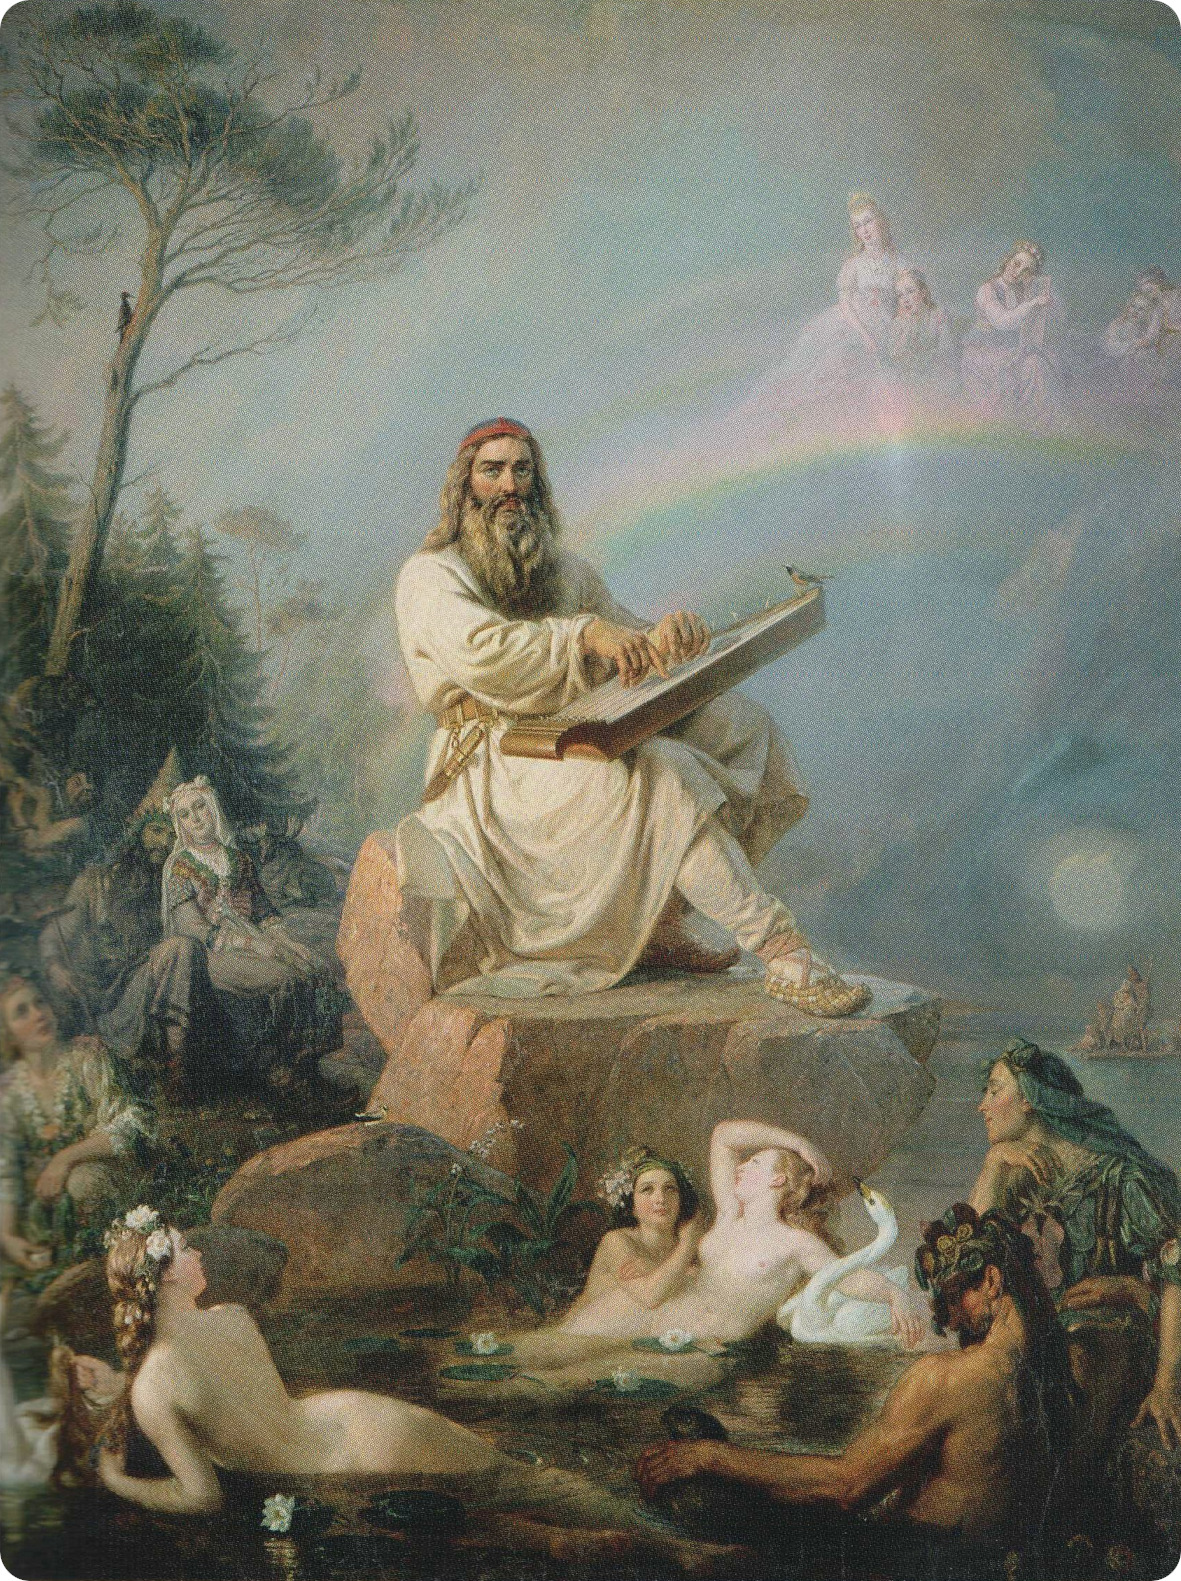
\includegraphics[width=0.82\textwidth]{Ekman_-_Vainamoisen_soitto.jpg}%
  \caption{R. W. Ekman: Väinämöisen soitto (1866)}%
\end{figure}
\vfill%


\clearpage
\subsection{Luonnon nostatus}
  \paragraph{}
  \begin{large}\begin{center}\begin{em}
    Luontoani nostattelen\\
    haastattelen haltijata\\
    Nouse luontoni lovesta\\
    Syntyni syvästä maasta\\
    Syntyni syvästä maasta\\
    \vspace{1em}
    Maasta hauna haltijani\\
    Nouse niin kuin nousit ennen\\
    Minun nostatellessani\\
    \vspace{1em}
    Isoni luonto, emoni luonto\\
    Luonto valta vanhempani\\
    Oman luontoni lisäksi\\
    Nosta Ukon voima taivahasta\\
    Maasta maan Emoisen voima\\
    \vspace{1em}
    Tuekseni turvakseni väekseni voimakseni\\
    Tulkaa tarvittaessa, käykää kutsuttaessa\\
    Terveyttä tekemään rauhaa rakentamaan\\
    \vspace{1em}
  \end{em}\end{center}\end{large}

  \paragraph{}
  %\begin{em}
    Eräs kielemme vanhimmista sanoista on ``noita'', joka on alunperin tarkoittanut tietäjää eli
    shamaania. Kristillisellä aikakaudella noita sai kielteisen kaiun. Sitä ennen tietäjät
    olivat arvokas osa yhteisöä, jonka jäseniä he tukivat sairauksissa ja elämän murroskohdissa.
    \par
    Sekä loveen lankeaminen että haltioituminen ovat tietäjien tapoja saavuttaa taianomainen
    mielentila, jossa he saavat apua esivanhemmiltaan tai suojelushengiltä.
  %\end{em}

  \paragraph{Lovi} on yliluonnollinen paikka tai olotila, aukko arkitodellisuuden ja alisen
    maailman välillä. Aliseen maailmaan kuuluu vainajala taikka Tuonela, jossa esi-isät asustavat.
    Lovi sijaitsee joko maan tai veden alla --- ilmeisesti myös naisten hameen alla, sillä
    kansanrunojen mukaan sieltäkin löytyy ovi tuonpuoleiseen. Osa muinaisista hautajaistavoistakin
    viittaa siihen, että vainaja pyrittiin palauttamaan takaisin kohtuun. Vainajalle tehtiin
    vertauskuvallisesti se, mitä sielulle toivottiin käyvän.
    \par
    Pohjolan emäntä Louhi, mahtava noita, tunnetaan myös muun muassa nimillä Lovetar ja Loviatar.
    Lovetar ilmenee syntysanoissa ja loitsun sanoissa. Louhi pystyy muuttamaan muotoaan,
    parantamaan, käskemään säätä, kuuta ja aurinkoa sekä synnyttämään mitä ihmeellisimpiä olentoja.
    Hänen kotinsa, myyttinen Pohjola, on pahojen asioiden, sairauden ja pakkasen lähde. Monet
    Pohjolan ongelmat, sairaudet ja harmit ovat itse Louhesta lähtöisin.
  \paragraph{Loveen lankeaminen:} Tietäjän matkaa vainajalaan kutsutaan loveen lankeamiseksi.
    Hurmoksessa tietäjä tekee sielunmatkan tuonpuolei\-seen ja käy kysymässä neuvoa esivanhemmilta.
    Suomalaiset tietäjät saattoivat vajota hurmokseen esimerkiksi raivoamalla, kun taas saamelainen
    \emph{noaidi} käytti apunaan rumpua. Loveen lankeamisessa käytettiin ehkä apuna myös laulamista
    [vrt. Väinämöinen laulaa Joukahaisen (Lapin tietäjän) suohon] ja soittamista (Väinämöisen
    jättihauenluinen kannel, jota kuunnelleessaan luomakunta lumoutui ja liikuttui).
    \par
    Väinämöinen lähtee Tuonelaan hakemaan puuttuvaa tietoa veneen rakentamiseen tai reen
    korjaamiseen. Joissain kertomuksissa hän hakee myös työvälineitä. Matkaa Tuonelaan
    kuvataan hyvin vaikeaksi ja vaivalloiseksi. Poiskaan sieltä ei ole helppo päästä, mutta
    Väinämöinen pakenee muuttumalla vesikäärmeeksi ja uimalla Tuonelan joen ylitse. Tämä
    viitannee muutokseen sieluneläimeksi, joiden joukossa käärmeet olivat suosittuja. Muutos
    sieluneläimeksi on yksi tietäjän keinoista.
  \paragraph{Lovesta nosto:} Loitsimalla saatetaan nostaa suvun esivanhempia eli omakuntaisia
    vainajalasta tälle puolen esimerkiksi suojelushaltijoiksi eli luonnoiksi.
  \paragraph{Luonto} on ihmisen tai muun tietoiseksi koetun olennon tai asian suojelushaltija.
    Alkuperäiseen merkitykseen viittaa ajatus jonkun luontumisesta. Luonnon katsotaann
    seuraavan ihmistä, suojelevan häntä ja tuovan hänelle onnea. Voimakasluontoiset eli ne,
    joilla on voimakas oma haltija, pärjäävät elämässä heikkoluontoisia paremmin. Luonto
    saattaa olla esimerkiksi vainajasta peräisin oleva esivanhempi eli \emph{syntyinen}.
  \paragraph{Luonnon kutsunta:} Jos ihmisellä on heikko luonto, hän saattaa joko kutsua itselleen
    vahvempaa luontoa tai voimistaa ja karaista luontoaan. Luontoa kutsutaan myös kateita,
    vihollisia ja sairauksia vastaan, ja antamaan lisää ruumiillisia, henkisiä tai yliluonnollisia
    kykyjä.
    \par
    Loitsuissa luonto nostetaan yleensä lovesta tai syvästä paikasta, vainajalasta. Joskus sitä
    kutsutaan nousemaan haon eli uppopuun alta. Joskus taas luontoa kutsutaan nousemaan ``haudan
    alta'', joka sekin viittaa siihen, että luonto on vainajalasta.
    \par
    Erään tiedon mukaan luontoaan saattaa karaista siten, että kohottaa juhlayönä järvestä hakoa
    ja kutsuu loitsulla luontoaan.
    \par
    Luontoa puhuteltaessa hänet ilmaistaan usein haltijaksi ja synnyksi. Tässä synty merkitsee
    joko myyttistä syntyä, esivanhemman sielua syntyistä tai molempia. Esimerkki loitsusta:

    \begin{center}\begin{em}
      Nouse luontoni lovesta,\\
      Syntyni syvästä maasta,\\
      Ha'on alta haltijani\\
      Vastuksia voittamah,\\
      Katehia kaatamah,\\
      Sotisia sortamahan\ldots\\
    \end{em}\end{center}

  \paragraph{Haltioituminen:} Ihmisen haltioituessa hänen luontonsa eli haltijansa hallitsee
    häntä. Tietäjät saattavat tavoitella haltioitumisen tilaa sairauksia parantaakseen tai
    muihin yliluonnollisiin tehtäviin.
    \par
    Nykyajan psykologiassa haltioituminen vertautuu lähinnä niin sanottuun flow-tilaan, jossa
    ihminen on syvästi keskittynyt tavoitteisiinsa. Joskus haltioituminen on käsitetty myös
    loveen lankeamisen vastineeksi tai taikojen harjoittamiseksi.
  \paragraph{Emuu} on olento, joka on synnyttänyt tai luonut jonkin kasvi- tai eläinlajin ---
    sen \emph{kantavanhempi} --- ja vastuussa tämän lajin toiminnasta sekä huolenpidosta.
    \par
    Metsästäjät pyytävät loitsuin kantavanhemmilta metsästysonnea. Pahaa voidaan yrittää karkottaa
    vanhempansa luo, tai uhata, että jos olento ei tottele, hänen käytöksestään kerrotaan hänen
    vanhemmalleen. Myös kantavanhempaa saatetaan käskeä panemaan lapsensa kuriin.
  \paragraph{Herättäjä} herättää ihmisen vaaran uhatessa. Jotkut väittävät omistavansa oman
    herättäjän, joka valvoo heidän untaan.
  \paragraph{Juhlia:} Nykyisistä juhlapyhistä laskiainen, helasunnuntai, juhannus, pyhäinpäivä ja 
    joulu olivat alun perin suomalaiseen alkuperäisuskontoon kuuluneita juhlia.


\subsection{Päivä, aurinko, kuu}

  \paragraph{Päivätär ja Kuutar:} Päivätär on elämää ja valoa hallitseva lämpöä ja hedelmällisyyttä
    antava hahmo. Kristillisellä kaudella hänet korvasi Neitsyt Maria. Hän on auringon ja päivän
    jumalatar, kaunis neito, jonka toveri tai kaksois\-olento on yhtä lailla kaunis kuun jumalatar
    Kuutar.
    \par
    Päivätär ja Kuutar omistavat auringon hopeaa ja kuun kultaa, joita näkyy kuun ja auringon
    hohteessa ja kultareunaisissa pilvissä auringonlaskun aikaan. Päivätär ja Kuutar näkyvät
    toisinaan Pohjolan tyttärien tavoin taivaalla kehräämässä kulta- ja hopealankaa kutoen
    siitä kultaisia ja hopeisia koruja ja vaatteita, joita neidot pyytävät kaunistuksekseen.

  \paragraph{Ilmarisen} mainitaan olleen mukana kosmisessa luomisessa, takomalla taivaankantta
    ja asettamalla taivaankappaleita.

  \begin{center}\begin{em}
    Tuli vanha Väinämöinen, ovelle asetteleikse.\\
    Sanan virkkoi, noin nimesi: ``Oi on seppo veikkoseni!\\
    Mitä paukutat pajassa, ajan kaiken kalkuttelet?''\\
    Se on seppo Ilmarinen sanan virkkoi, noin nimesi:\\
    ``Kuuta kullaista kuvoan, hope'ista aurinkoa\\
    tuonne taivahan laelle, päälle kuuen kirjokannen.''\\
  \end{em}\end{center}


\subsection{Maa}

  \paragraph{Akka} on Ukko ylijumalan nainen. Joskus hänet on tulkittu hedelmällisyyden
    jumalattareksi. Akka on luonnon naisellinen puoli, maaemonen, jonka Ukko hedelmöittää,
    ja sade saa viheriöimään. Näin saatiin aikaan maanviljelyn kannalta suotuisat ilmat.
    Akan mukaan on nimetty asteroidi \emph{8034 Akka}.
  \paragraph{Maan haltija} on nais- tai miespuolinen perhettä, taloa, satoa, karjaa ja pihapiiriä
    hoitava ja vartioiva hyvä haltija. Jos se on naispuolinen, menestyy karja hyvin, jos
    miespuolinen, menestyvät hevoset. Joskus haltijoita on pariskunta. Tällöin talo on erityisen
    onnekas.
    \par
    Haltijaa tulee kunnioittaa, niin hän hoitaa työnsä hyvin. Haltijalle on usein luvattu, että
    joka vuosi jonkun juhlan aikaan se saa osansa juhlaruuasta tai sadosta. Pyhä pihapuu on
    uhripaikka, jonka luona haltijaa kumarretaan ja sille viedään uhrilahjoja.
    \par
    Jos haltija on tavatessa hyvissä vaatteissa ja iloinen, ei hän ole onnettomuuden aiheuttaja,
    ja on vain varoittamassa. Jos haltija on pahoissa vaatteissa eikä näytä kasvojaan, on hän
    vihastunut, ja aikomassa aiheuttaa onnettomuuden. Erään perinteen mukaan tällöin on kiireesti
    mentävä paikalle, jossa haltija on näyttäytynyt, ja uhrattava alasti.
    \par
    Kun perustetaan uutta taloa, tehdään taikoja, jotta saataisiin haltija. Muuten voivat pahat
    haltijat tai maanväki asettua pihapiiriin. Erään kansanperinteen mukaan mukaan pitää polttaa
    tulta kolme päivää sillä paikalla, johon haluaa talon perustaa. Kolmantena päivänä haltija
    ilmestyy unessa. Silloin näkee, tuleeko mies- vai naishaltija vaiko pariskunta.
  \paragraph{Maahiset} eli \textbf{maanväki} ovat pieniä, ihmisenmuotoisia olentoja, jotka asuvat
    maan alla omassa maailmassaan. Usein maahisten maailma koetaan todellisen maailman
    peilikuvaksi, joka voi olla ylösalaisin.
    \par
    Maahiset voivat olla ilkikurisia. Metsässä saattaa joutua maahisten lumoihin ja eksyä
    nurinkuriseen maailmaan, jota \emph{metsänpeitoksikin} on kutsuttu. Maan väki voidaan käsittää
    myös taikavoimaksi, jota on maassa. Maanpäällisessä maailmassa maahiset ovat yleensä
    näkymättömiä. Maahisten kerrotaan myös lumoavan ihmisiä jäämään luokseen, jos ottaa vastaan
    heidän tarjoamiaan lahjoja, ruokaa tai juomaa.
  \paragraph{Sampsa Pellervoinen} kylvää maan kasvillisuuden, kaikenlaiset metsät, suot, ahot ja
    kivikotkin. Kylvö tapahtuu sammon murusten avulla. Hän on hedelmällisyyden haltija; hänet on
    rituaalisesti herätettävä joka kevät.
  \paragraph{Äkräs} on monipuolinen kasvillisuuden haltija. \emph{Loi herneet, pavut ja nauriit
    sekä antoi kaalit, pellavat ja hamput: Egres hernet Pawudh Naurit loi / Caalit Linat ia Hamput
    edestoi.}
  \paragraph{Jumi} on yliluonnollisten ilmiöiden, lähinnä panteistisen maailmanhengen nimitys.
    \emph{Marit} (volgansuomalainen kansa) viettävät vuosittain Jumolle omistettua juhlapäivää
    uhraten lihaa ja viljaa. Jumi aiheuttaa esimerkiksi eläimelle äkillisen taudin ampumalla
    näkymättömän nuolen. Arvoituksissa jumi on jokin, jolle on ominaista ehdoton paikallaanolo
    tai jota on mahdoton kiertää.

  % \subsubsection{Kivet}
    \paragraph{Kyllikki:} kivien emuu loitsuissa, joilla kiven aiheuttamia vammoja hoidetaan
  % \subsubsection{Käärme}
    \paragraph{Käres:} käärmeitten emuu
    \paragraph{Mammotar:} matojen emuu


\subsection{Meri ja vesi}

  \paragraph{Ahti:} veden jumala tai haltija
  \paragraph{Vellamo, Veen emonen, Veden emo} on hyvä ja arvostettu vedenhaltija, joka asuu veden
    alla Ahtolassa ja on Ahdin puoliso. Häntä palvotaan kalansaaliin toivossa ja purjehdussäähän
    vaikuttamaan.
    \par
    Vellamo on kaunis; hänellä on sininen lakki, kaislainen paita ja vaahtoinen vaippa.
  \paragraph{Iku-Turso} (myös \textbf{Meritursas} ja \textbf{Iku Turilas}) on vedenhaltija tai
    merihirviö, jonkinlainen alkuolento, joka on ollut olemassa maailman syntymästä lähtien.
    Runoissa se esiintyy usein Ison Tammen, maailmanpuun, kanssa.
  \paragraph{Väinämöinen}-nimen uskotaan juontuvan väinä-sanasta, joka tarkoittaa suvantoa tai
    hiljalleen virtaavaa vettä, salmea tai joensuuta. Väinämöisen lisämääreenä esiintyy myös
    \textbf{suvantolainen}.
    \par
    Väinämöinen on Ilmattaren, ilman immen ja meren poika. Hän viettää meressä kelluvan äitinsä
    kohdussa kolmekymmentä vuotta ja alkaa synnyttyään autella maailman luomisessa.
    \par
    Väinämöinen on taidokas veneenveistäjä. Hän tietää melkein kaiken tarpeellisen veneen tekoon,
    mutta ei kolmea ratkaisevan tärkeää sanaa, luotetta. Hän lähtee hakemaan niitä Tuonelasta,
    kuolleiden maasta. Väinämöinen käy myös ammoin kuolleen tietäjä Vipusen vatsassa tietoa
    hakemassa. Matka kuolleiden maahan on kuviteltu hyvin vaaralliseksi, vain mahtavien
    tietäjien on ajateltu pystyvän siihen ja tulemaan takaisin. Tässä on uistumia rituaaleista,
    joissa tietäjä vajoaa transsiin, ja hänen sielunsa liikkuu kuolleiden maailmassa suorittamassa
    tehtävää; suomalaisessa mytologiassa kerrotaan loveen lankeamisesta ja lovesta nostosta.
    \par
    Tuonen tytti toimii lautturina ja saattaa veneellään vainajat Tuonen mustan virran yli.
    Väinämöisen tytti kuitenkin huomaa olevan elossa. Väinämöinen valehtelee kuolleensa, mutta ei
    vakuuta. Tytti tietää millaisia ovat eri tavoin kuolleet: rautaan kuolleet ovat verisiä,
    hukkuneet vetisiä ja palaneet kärventyneitä. Väinämöinen kuitenkin lopulta pääsee Tuonelle.
    Tuonella hänet laitetaan nukkumaan vastenmieliseen sänkyyn tai paikkaan, joka on tehty
    käärmeistä tai täynnä käärmeitä. Hän onnistuu kuitenkin pakenemaan. Hän muuttuu vesieläimeksi,
    ja ui Tuonen joen poikki. Tuonen poika virittää rautaverkon veteen, mutta ei saa Väinämöistä
    tarttumaan. Väinämöinen palaa Tuonelta saatuaan haluamansa ja kertoo eläville Tuonelan
    oloista.
    \par
    Joissain runoissa kerrotaan, että Väinämöinen menee veneellään Rutjan koskeen, tuliseen
    pyörteeseen. Pyörre on usein tulkittu reitiksi Tuonelaan, vauhdikkaammaksi versioksi Tuonen
    joesta. Väinämöinen menee siis elävänä kuolleiden maahan. Väinämöisen veneenjäljeksi kutsutaan
    tyyntä kohtaa muuten aaltoilevalla vedenpinnalla.
    \par
    Vedenpinnan nimitysten lisäksi Väinämöiseen liittyviä nimityksiä löytyy luonnosta
    tähtitaivaalta, kuten Väinämöisen miekka tai viikate (Orion) ja Väinämöiset tai Väinämöisen
    virsut (Seulaset). Näitä tähdistöjä on käytetty suunnistamiseen vesillä. Väinämöisen
    arvellaankin alun perin liittyneen kiinteästi vesillä liikkumiseen.
    \par
    Kalevalassa Väinämöinen syntyy Ilmattaresta vanhana miehenä. Kansanrunoissa Ilmatar ei synnytä
    Väinämöistä, vaan Väinämöinen syntyy joko yksin tai Iro-neidosta.


\subsection{Ukkonen ja tuli}

    Samanistisessa kosmologiassa ihmisen maailma sijaitsee henkien asuttamien monikerroksisten ylä-
    ja alamaailmojen välissä. Joissain kansanrunoissa se kuvataan kodan pohjaksi, josta
    taivaankupoli rajaa henkien asuinsijat. Molemmissa ajatusrakennelmissa taivasta kannattaa
    maailmanpylväs ja taivaan napaa edustaa Pohjantähti.
    \par
    Käsitys sielusta kuuluu ikivanhaan pohjoiseen samanismiin. Sielun ja ruumiin pitkästä
    rinnakkaisuudesta kertoo muun muassa sukulaiskansojemme \emph{mansien} ja \emph{hantien} sana
    \emph{is}, joka on sukua suomen sanalle itse. Tähän liittyy löyly, joka sukukielissämme viittaa
    kylpemisen ohella sieluun.
  \paragraph{Ukko ylijumala} on muinainen sään ja sadon, ilman, oikeuden sekä ukkosen jumala, jota
    pyydetään avuksi esimerkiksi taisteluun tai taikuuteen ryhtyessä.
    \par
    Ukon lisänimen ``ylijumala'' voikin tulkita kahdella tapaa: joko, että hän todella on mahtavin
    (eli ylin), jumalista; tai pelkästään, että hän asuu ylhäällä taivaalla. Vahinkoa tekevän
    salamaniskun ajatellaan olevan Ukon rangaistus tai vihan ilmaus, ja elämää tuovan sateen
    hänen suopeutensa osoitus. Ukkoa muistuttava ukkosenjumala tunnettiin latvian kielessä nimellä
    \emph{Perkons} ja liettuan kielessä nimellä \emph{Perkūnas}, joista on peräisin suomen sana
    Perkele.
    \par
    Ukko iskee salamoita kirveellä, vasaralla, nuolella tai miekalla. Kokonaisen ukonilman hän saa
    aikaan puimalla riihtä, kyntäen, jyristellen vaunuillaan taivaissa, makaamalla naispuolisen
    jumaluuden kanssa, taikka kolisuttamalla konkeloa eli kelopuuta. Savukvartsia, josta
    iskettäessä syntyy kipinöitä ja palaneen hajua, nimitetään ukonkiveksi.
    \par
    Ukko kävelee pitkin askelin pilvien ja monikerroksisen taivaan yläpuolella, ja katselee
    ylhäältä maailmaa. Mahtavuudestaan huolimatta Ukko ei ole kaikkitietävä tai kaikkivaltias, vaan
    muilla henkiolennoilla ja ihmisillä on valtaa ja toimintatilaa. Ukon taivaallisessa
    valtakunnassa on heikompia henkiolentoja, joista perinteet tuntevat muun muassa päivättäret,
    kuuttaret, ilman immet, kapeet, kuumet, tuulettaret ja muita.
    \par
    Ukon kerrotaan myös pitävän pilvissä käräjiä, joten voisi olettaa, että taivaalla asuu tai
    ainakin vierailee muitakin merkittäviä henkiolentoja, joiden kanssa Ukko päättää asioista.
    Ukkoa rukoillaan pitämään käräjiä eri ongelmien voittamiseksi.

  \paragraph{Kokko} tai \textbf{vaakalintu} on jättiläismäinen kotka, sukua yleismaailmalliselle
    ukkos\-lintuhengelle, joka tunnetaan Euroopasta aina Amerikan alkuperäiskansoille asti. Se
    voi olla muistumaa ihmishahmoista jumaluutta edeltäneestä käsityksestä, jonka mukaan taivasta
    ja ukkosta hallitsee ukkoslintu. Ukkoslintuihin uskovat paitsi jotkin suomalais-ugrilaiset,
    myös monet muut kansat.
    \par
    Kokon mittasuhteet kuvataan joskus valtaviksi: toinen siipi haroo taivasta, kun toinen
    koskettaa meren luotoja.
    \par
    Kokko ja Ilmarinen osallistuvat yhä joissain tulen syntysanoissa ensimmäisen tulen iskentään,
    joka toisissa perinteissä on Ukon tehtävä. Kokko on toisinaan tarusankarien ystävä, toisinaan
    vihollinen. Joskus sen tehtävä on vartioida. Kokko kuvataan joskus rautaiseksi, joskus
    tuliseksi. Kokko pystyy kantamaan ihmistä. Se iskee tulta auttaakseen Väinämöistä polttamaan
    kasken. Myös kokon sulkia käytetään tulen iskemiseen. Joissain tulen syntykertomuksissa tuli
    on isketty kokon sulilla.
    \par
    Kokkoja voi olla useita. Eräs näistä pelastaa Väinämöisen merihädästä palkkioksi siitä, että
    kaskea kaataessaan Väinämöinen jätti koivun linnuille istumapuuksi. Ilmarinen ja Louhi tekevät
    omat kokkonsa. Ilmarinen tekee metallisen kokon, joka pyydystää suomuhauen. Louhi taas muuttuu
    itse kokoksi rakentamalla siivet ja pyrstön laivan osista ja ottamalla viikatteet
    kynsiksi.
    \par
    Sanassa vaakalintu esiintyvä ``vaaka'' tulee mahdollisesti sanasta ``vaa’as'', joka tarkoittaa
    myyttistä tulta, aaltoa ja kipua. Toinen mahdollisuus on ``vuokko'', saamelaisten kertomusten
    tietäjän apulintu.
  \paragraph{Panu} on tulen henki, auringon poika. Panuun voi vedota loitsuissa, kun ollaan
    tekemisissä tulen kanssa.


\subsection{Ilma ja tuuli}

  \paragraph{Ilmattaret} eli \textbf{Ilman immet} ovat taivaalla asuvia jumalaisia neitoja, jotka
    muistuttavat Pohjan neitoja, sillä nekin istuvat ajoittain taivaankannella.
    \par
    Ilmatar liittyy Väinämöisen ja maailman syntymään. Ilmatar tylsistyy oloonsa impenä taivaalla
    ja laskeutuu meren selälle. Tuuli hedelmöittää hänet. Sotka etsii pesäpaikkaa ja huomaa
    Ilmattaren polven, jolle se tekee pesän ja munii siihen munansa. Polvea alkaa kuumottaa ja
    Ilmatar heilauttaa sitä, jolloin munat putoavat ja särkyvät. Särkyneistä munankuorista syntyy
    maailma.
  \paragraph{Seppo Ilmarinen} on Väinölässä asuva seppäsankari, jolla on jumalallisia piirteitä.
    Häntä pidetään myös tuulen, sään ja ilman jumalana, joka on mukana maailman syntymässä.
    \par
    Iro-neito synnytti Ilmarisen yöllä ja jo päivällä Ilmarinen teki pajan. Palkeet liittyvät
    Ilmarisen asemaan tuulen jumalana, mutta toisaalta myös tämän rooliin kosmisena seppänä.
    Ilmarisen taontatyö ei onnistu ennen kuin hän tarttuu palkeisiin orjien sijasta itse.
    Ilmarinen takoi maailman alussa taivaankantta niin taidokkaasti, etteivät näy pihtien pitämät,
    eivätkä tunnu vasaran iskut. Ilmarisen kädenjälkeä ovat myös revontulet, aamu- ja iltaruskon
    värit. Myös raudan keksiminen ja alkutulen iskeminen ovat Ilmarisen saavutuksia. Ilmarinen
    takoo monia esineitä, kuten Sammon, Kultaisen naisen, ja yrittää takoa uuden Auringon ja Kuun.
    \par
    Suomalaisilla lienee ollut Ukkoa aikaisempi, omaperäinen taivaan jumala. Tämän syrjäydyttyä
    Ukon tieltä siitä kehittyi kalevalaisen perinteen seppäsankari Ilmarinen. Ilmarisen asemasta
    taivaan jumaluutena on säilynyt muistumia myytteihin, kuten uskomukset, että hän takoi
    taivaankannen ja Sammon, joka alkujaan käsitettiin taivaan tukipylvääksi.
  \paragraph{Sielulintu} on sielun koti ja vertauskuva. Lintu ehkä tuo sielun syntymässä ja vie sen
    kuoleman hetkellä. Joidenkin perinteiden mukaan nukkuessa on hyvä olla lähellä puusta
    veistetty sielulintu, joka pitää huolta sielusta unen aikana, jottei se lähtisi omille
    teilleen. Ihmisen kuoltua hänen puinen sielulintunsa laitetaan ortodoksisen hautaristin
    yläpuolelle. Lintujen ruokkiminen jouluna on vanha tapa; kuolleet eli sielulinnut ovat elävien
    kanssa mukana keskitalven juhlassa.
    \par
    Samanistisessa ihmiskuvassa sielu on usein monikerroksinen. Sen osista yksi saattaa unessa tai
    transsissa liikkua kehon ulkopuolella esimerkiksi linnun hahmossa. Lintujen merkitys
    suomalais-ugrilaisille näkyy siinäkin, että taivaan halkaisevan galaktisen vyön nimi on
    Linnunrata.
  \paragraph{Tuuletar} tarkoittaa naispuolista tuulta hallitsevaa luonnonhenkeä tai tuulen
    personoitumaa. Tuulettaria on erilaisia. Tuuletar saattaa olla yksittäinen tuulenpuuska,
    vihuri tai tuulispää, tai tietynlainen jatkuva tuuli. Tuuletar voi myös olla tuulen jumala,
    jolta pyytämällä saa suotuisaa ilmaa. Tietty tuuletar voi myös vastata tietystä ilmansuunnasta
    tulevaa tuulta.
  \paragraph{Tapiotar:} lintujen emuu


\subsection{Metsä}

  \paragraph{Tapio} on metsän haltija ja hän hallitsee metsäistä valtakuntaansa Tapiolaa. Tapion
    väki kaunistaa ja siivoaa metsää, huolehtii kasveista ja eläimistä. Tapion tyttäriä ovat
    ihastuttavat Tellervo, Tyytikki, Tuulikki ja Annikki. Tapiota ja hänen perhettään kuvaillaan
    ihmishahmoisiksi ja joko alastomiksi tai kauniisti pukeutuneiksi. Joidenkin runojen mukaan
    Tapion parta on puuta ja silmät kuin kaksi pohjatonta järveä.
  \paragraph{Mielikki} on Tapion vaimo. Metsästäjien on puheltava ja laulettava viettelevästi ja
    imartelevasti Mielikille saadakseen tältä lahjana saalista. Mielikki hoitaa metsän ``taloustyöt''
    eli siistimisen, koristelun ja kaunistamisen. Metsän kauneutta, kuten myös Mielikin omaa
    kauneutta, kannattaa metsässä liikkuessa kehua. Mielikin uskotaan lepyttävän miestään Tapiota,
    jos tämä tulee huonolle tuulelle ja usuttaa voimat metsämiehiä vastaan.
    \par
    Harvoin ihmisille näyttäytyessään Mielikki usein huvikseen pukeutuu Tapion harmaaseen
    naavaturkkiin ja -hattuun. Katsojan silmissä kuu\-sikossa kulkee höperö vanhus, joka laskee
    mättäiden marjoja.
    \par
    Mielikki on taitava parantaja. Hän hoitaa ansoihin jääneet käpälät ja tassut, pesästä pudonneet
    linnunpoikaset ja metsokukkojen taisteluhaavat. Metsän parantavat kasvit hän kerää
    huolellisesti talteen, ja niinpä hänellä on sopivia rohtoja myös ihmisten vaivoihin, jos joku
    vain keksii käydä pyytämässä. Mielikin käyttämiä kasveja ovat muun muassa kanerva ja kataja.
    \par
    Pienriistan pyytäjän, sienestäjän ja marjastajan kannattaa lausua metsään mennessään:
    \emph{``Siniviitta, viidan eukko, / mieluinen metsän e\-mäntä! / Anna tie, avaa portti / minun
    metsällä käydessäni.''} Mielikin nimi juontuu onnea ja kohtaloa merkinneestä mielu-sanasta.
  \paragraph{Tyytikki:} oravien emuu; Tapion ja hänen puolisonsa Mielikin tytär
  \paragraph{Metsän haltijat ja olennot:} Metsässä on myös arvaamattomampia tai vihamielisiä
    olentoja, kuten maahisia, metsähiisiä, menninkäisiä ja keijuja. Nämä saattavat sairastuttaa,
    eksyttää tai lumota, jos tulee näiden valtapiirille. Menninkäiset saattavat eksyttää metsässä
    kulkevan nurinkuriseen maailmaan. Metsässä saattaa olla myös noidankehä, alue, johon joutunut
    lumoutuu. Tätä saattaa merkitä esimerkiksi sienien itiöemien muodostama kehä.
    \par
    Metsän väkeä asuu muun muassa muurahaiskeoissa, puunkoloissa, kivenkoloissa, juurakoissa ja
    kannoissa. Väen taikavoimaa saattaa löytää myrskyn katkaisemien puiden murtumakohdista tai
    yhteenkasvaneista puista. Avoimella paikalla kasvava yksinäinen puu on tärkeä metsänväen
    kokoontumispaikka.
  \paragraph{Metsänneito} (myös \textbf{metsänneitsyt}, \textbf{metsänpiika}, \textbf{sinipiika})
    ilmaantuu joskus metsässä liikkuville tai yöpyville miehille: se saattaa tulla tanssimaan
    nuotiolle tai kävellä vastaan. Metsänneitsyt oli edestäpäin ihastuttavan kaunis, harsopukuinen
    ja pitkähiuksinen, mutta olennon selkäpuoli on ontto tai takaa se on vain puupökkelö. Tämän
    huomaaa kauhukseen mies, jos yrittää nähdä neidon selkäpuolen. Tällöin metsänneitsyt pelästyy
    ja lähtee.
  \paragraph{Menninkäinen} on yksinäisillä paikoilla asustava pieni ja pimeästä pitävä olento, joka
    on yleensä ihmisille suopea. Sana on ilmeisesti alun perin tarkoittanut vainajaa ja manalaista.
    Menninkäiset eivät välttämättä kestä päivänvaloa. Ne ovat vieraita ja outoja olentoja, joiden
    motiivit ovat ihmisille tuntemattomat, päin vastoin kuin tiettyihin elementteihin liittyvien
    väkien.
    \par
    Menninkäiset ovat voineet tulla mellastamaan kirkkoon öisin, jolloin niitä on pidetty pikku
    paholaisina. Ne saattavat pälyillä ihmisiä ikkunan tai puunrungon takaa, tai istuskella ryhmänä
    kivellä ihmistä tuijottaen. Menninkäiset järjestävät mielellään pitoja, joissa syödään, juodaan
    ja tanssitaan. Menninkäiset pitävät kiiltävistä esineistä.
  \paragraph{Ajattara:} paha naispuolinen olento, joka ajaa metsämiehiä ja metsästäjiä harhaan.
  \paragraph{Hongatar:} ärtyisä ja rujo karhujen emuu, honkien suojelija
  \paragraph{Juonetar:} peurojen emuu
  \paragraph{Käreitär:} kettujen emuu
  \paragraph{Laus:} porojen ja hirvien emuu
  \paragraph{Äimätär:} susien emuu


\subsection{Puut}

  \paragraph{Kati:} puiden emuu --- metsän kaunis ja nuori jumalatar, joka synnyttää puita
  \paragraph{Elämänpuu:} Nainen nähdään elämän ja kuoleman sekä niitä vastaavien ilmansuuntien
    etelän ja pohjoisen hallitsijana. Tämän äitihahmon mielikuvastoon liittyvät myös aurinko ja
    elämänpuu, joka usein mielletään koivuksi.
    \par
    Kalevalassa Iso Tammi kohoaa peittämään koko taivaankannen ja se lopulta kaadetaan. Aihelmaa
    on selitetty Linnunradan syntynä, sillä Linnunrata muistuttaa muodoltaan kaadettua puuta.
  \paragraph{Koivu:} \emph{[vesi]} suojelu, puhdistaminen. Koivunoksia on käytetty kautta aikain
    karkottamaan pahoja henkiä ihmisestä vihtomalla.
  \paragraph{Poppeli:} \emph{[vesi]} vauraus, lentäminen
  \paragraph{Haapa:} \emph{[ilma]} suojelee varkauksilta, parantaa ilmaisukykyä
  \paragraph{Mänty:} \emph{[ilma]} parantaminen, hedelmällisyys, vauraus
  \paragraph{Pihlaja:} \emph{[tuli]} psyykkiset voimat, parantaminen, voima, menestyminen, suojelu
  \paragraph{Tammi:} \emph{[tuli]} suojelu, terveys, vauraus, paraneminen, potenssi,
    hedelmällisyys, onni
  \paragraph{Saarni:} \emph{[tuli]} suojelu, terveys, mereen liittyvät rituaalit, vauraus
  \paragraph{Kataja:} \emph{[tuli]} suojelu, varkauksien esto, rakkaus, terveys


\subsection{Tieto}

  \paragraph{Antero Vipunen} on maan alla makaava vainaja tai jättiläinen; tietäjä, jolla on
    hallussaan arvokkaita ikiaikaisia loitsuja tai tietoja.
    \par
    Väinämöisen loitsusta puuttuu kolme sanaa eli luotetta. Ne saadakseen hän menee herättämään
    nukkuvan Vipusen joko hakkaamalla puut tämän haudalta tai menemällä suusta vatsaan. Vipunen
    voi myös nielaista Väinämöisen. Vatsassa Väinämöinen takoo niin kovasti, että Vipunen
    luovuttaa ja antaa sanat vatsakivusta päästäkseen.
    \par
    Viron kielessä \emph{vibu} on jousipyssy, joten Virossa Vipunen on käsitetty taitavaksi
    jousimieheksi. Useissa kertomuksen versioissa Vipusen mainitaan olevan ansastaja, kuten
    nimestä Vipunen voi päätellä. Vipusen arvellaan lainatun saamelaisista tarinoista, joissa
    käytiin noita Antereeuksen haudalla hakemassa tietoja.
  \paragraph{Väinämöinen} on taidokas loitsujen laulaja, kanteleen soittaja ja suuri tietäjä:
    \emph{``Vaka vanha Väinämöinen / Tietäjä iän ikuinen''}. Hän veistää veneen laulamalla.
    \par
    Sotajoukon laiva pysähtyy jättiläismäisen suomuhauen selkään. Hauki tapetaan, ja sen
    leukaluusta Väinämöinen tekee kanteleen. Kanteleen kielet hän saa jonkin Hiiden olennon
    hiuksista. Väinämöinen soittaa kanneltaan niin taidokkaasti, että ihmiset, eläimet ja
    jumalolennotkin tulevat kuuntelemaan, eikä ole karskeintakaan urosta, joka ei liikuttuisi
    kyyneliin.
    \par
    Eräässä yleisessä kansanrunossa Väinämöinen syntyy yöllä, tekee päivällä pajan, takoo
    rautaisen hevosen, ja ratsastaa sillä veden päällä. Joukahainen on nuori ja laiha Lapin
    tietäjä, joka kadehtii Väinämöisen laulutaitoja ja matkustaa kolme päivää haastamaan tämän
    miekan mittelöön. Väinämöinen ei suostu miekkailemaan. He loihtivat kilpaa, jonka päätteeksi
    Väinämöinen laulaa Joukahaisen suohon. Pelastautuakseen Joukahainen lupaaa Väinämöiselle
    siskonsa Ainon puolisoksi. Aino hukuttautuu, sillä hän ei halua vaimoksi vanhalle
    Väinämöiselle. Väinämöinen ratsastaa veden päällä, ja Joukahainen ampuu hänet kostoksi
    alkumereen.
    \par
    Aiemmissa runoissa Väinämöinen ja Joukahainen ovat saman äidin, Iro-neidon lapsia. He lähtevät
    yhtä matkaa kulkemaan, mutta ajautuvat erilleen ja käyvät toistensa kimppuun. Väinämöinen
    voittaa taikansa avulla. Maailmankaikkeus syntyy, kun sotka munii munansa Väinämämöisen
    polvelle Joukahaisen suistettua hänet veteen. Väinämöinen kelluu vedessä, kun vesilintu, sotka,
    pesii hänen polvelleen. Haudonta polttaa polvea, jolloin Väinämöinen vavahduttaa sitä.
    Linnun munat joutuvat mereen, hajoavat ja synnyttävät maailman. Kalevalassa sotka munii
    Väinämöistä odottavan ilmattaren polvelle, eikä Väinämöisen polvelle, kuten kansanrunoissa.
  \paragraph{Väinämöisen paluu?} Neitsyt Marjatta tulee raskaaksi puolukasta ja saa poikalapsen
    tai lapsi löytyy metsästä, jolloin etsitään turhaan myös äitiä. Väinämöinen määrää lapsen
    äpäränä suolle vietäväksi ja puulla päähän lyötäväksi. Sylilapsi alkaa puhua, syyttää
    Väinämöistä pahemmista synneistä ja huomauttaa, ettei Väinämöistäkään ole niiden takia viety
    suolle. Lapsi kastetaan Kaukomieleksi Karjalan kuninkaaksi.
    \par
    Väinämöinen suuttuu, häpeää ja poistuu vaskisella ja kuparisella veneellään, ja sanoo
    palaavansa, kun häntä tarvitaan, etsitään ja kaivataan. Samaan tapaan vesitse ja kristinuskon
    ahdistamina ovat poistuneet myös Kalevanpojat, mutta he soutivat kivellä.


\subsection{Hiisi}

  Hiisi on pyhä kulttipaikka, pyhä lehto ja mahdollisesti kalmisto. Hiideksi on myös myöhemmin
  alettu kutsua kulttipaikalla palvottua henkiolentoa, kalmiston vainajien yhteensulautuneiden
  henkien muodostamaa kollektiivia.
  \par
  Kristinuskon saapumisen jälkeen hiisi on ollut paha henkiolento ja paha paikka. Hiisistä
  muodostui kansantarinoihin pieniä pahoja tai vähintään tuhmia olentoja, joiden kotipaikka oli
  myös nimeltään Hiisi, tai joskus Hiitola. Metsähiisi ja vesihiisi olivat metsässä ja vedessä
  asuvia hiisiä, mutta myös sairauksien nimiä. Myös pyhästä hauta-alueesta tai helvetin kaltaisesta
  paikasta saatettiin puhua hiitenä. Myöhemmin hiisi-sana alkoi viitata pakanalliseen
  henkiolentoon, pienikokoiseen ilkeään haltiaan tai peikkoon.
  \par
  Kalevalassa Väinämöinen joutuu taistelemaan Lempoa, Pahaa ja Hiittä vastaan. Hiisien kotipaikka
  Hiitola sijaitsee vaikeakulkuisessa maastossa, syrjässä ihmisasutuksesta. Hiittä pahana paikkana
  on peräpohjolassa kutsuttu sanalla helsinki. Joskus hiisi rinnastetaan myös jättiläisiin tai
  vuorenpeikkoihin.
  \par
  Hiitolaan on rakennettu Hiiden linna, jossa Hiisi asuu Hiiden emännän kanssa. Hiiden emännältä
  Väinämöinen saa kanteleeseensa kielet. Hiiden linnassa asuu myös hiitolaisia --- joiden hiukset
  olivat käärmeitä --- sekä Hiiden raivoava rakki ja Hiiden kissa, Kipinätär nimeltään. Hiidellä
  on myös Hiiden ruuna, hiisien nopea hevonen ja yksi ainoa tytär, Hippe. Hipen tehtävänä on
  laittaa varkaat palauttamaan varastettu omaisuus oikeille omistajilleen. 

  \paragraph{Hiiden hirvi} on vaikeasti pyydystettävä, voimakas ja nopea hirveä muistuttava olento.
    Se saattaa olla samaa kantaa kuin samojedien ja obinugrilaisten taivaallinen peura,
    kuusijalkainen olento, jonka ensimmäinen samaani pyydysti. 


\subsection{Pohjola}

  Pohjolan emännän valtakunta kuvataan pahaksi ja kylmäksi maaksi kaukana pohjoisessa. Pohjola
  on sekä sankarien vihollinen, että pahojen asioiden, kuten pakkasen ja sairauksien, alkulähde.
  Pohjolan hyviä oloja kuitenkin kadehditaan, eivätkä kielteiset käsitykset estä kalevalaisia
  sankareita matkaamasta kohti Louhen valtakuntaa ja kosiskelemasta hänen yliluonnollisen kauniita
  tyttäriään.

  \paragraph{Pohjolan emäntä} eli \textbf{Pohjan akka} johtaa myyttistä Pohjolaa. Kalevalassa
  Pohjolan emännän nimi on \textbf{Louhi}, mutta tunnetaan muitakin nimiä: \textbf{Lovetar},
  \textbf{Loviatar}, \textbf{Louheatar} ja \textbf{Lovehetar}. Häneen viitataan säeparilla:
  \emph{``Louhi Pohjolan emäntä / Pohjan akka harvahammas''}.
  \par
  Pohjolan emännällä on suunnattomat taikavoimat: hän pystyy muuttamaan muotoaan, käskemään säätä,
  säätämään auringon ja kuun kulkua, parantamaan ja on kykeneväinen synnyttämään mitä
  ihmeellisimpiä olioita. Hän varustaa sotaveneen soutajineen ja sotaväkineen, ja veneen
  tuhouduttua ottaa veneen laidat siivikseen, ja muuntautuu jättimäiseksi Kokko-linnuksi, jonka
  selkään soturit nousevat.
  \par
  Pohjolan emäntä on synnyttänyt monia ongelmista, jotka tulevat Pohjolasta ihmisten harmiksi.
  Hänet on usein portoksi mainittu siksi, etteivät nämä ``lapset'' ole avioliitosta peräisin. Hänet
  hedelmöittää tuuli, kun hän paljastaa alapäänsä pohjoiseen päin, tai sen tekee Iku-Turso meren
  kuohuilla kovilla.
  \par
  Louhi mainitaan usein myös ihmeellisten Pohjolan neitojen äidiksi. Pohjolan isäntä jää yleensä
  sivuosaan. Yleensä miestä ei mainita ollenkaan, ja paheksuen korostetaan, että emäntä luo
  synnyttämänsä asiat ja olennot luonnottomasti ja aviottomasti.


\subsection{Sampo}

  Sampo on ihmeellinen, rikkauksia tekevä mylly: kirjokansi, ihmekone, joka jauhaa rahaa, viljaa ja
  suolaa. Sampo jauhaa, sillä maailmanpylvään on ajateltu kiertyvän taivaankannen mukana. Sillä
  arvellaan myös olevan jalat, joiden avulla se seisoo, sekä reiät tai nokat. Sammon juuret ovat
  syvällä maaemässä, ja Sammon yleinen toisintonimi on kirjokansi, joka viittaa taivaankanteen.
  Sammas on patsas, joka kannattaa taivaan kantta. Kultanappi tai kultainen naula on pohjantähti
  (tai Vega, joka oli 12 000 vuotta sitten Pohjantähden kohdalla), joka kiinnittää taivaankannen
  ja maan. Taivaankansi pyörii naulan ympäri: ``sammas jauhaa''. Myös indoeurooppalaisilla kansoilla
  on maailmanpylväsmyytti. Esimerkiksi Intiassa pylvästä kannattelee kilpikonna.
  \par
  Sampo-tarut ovat, paitsi ihmeellisiä kertomuksia kahden kansan taistelusta ja ihme-esineen
  vaiheista, alkujaan kosmisia kuvauksia. Ne selittävät maanviljelyksen syntyä ja muidenkin
  asioiden myyttistä alkuperää. Sampo on esiintynyt myös nimillä sampa, sammas, sampi, sampu,
  samppu, samppo ja sammut. Sanana sampo on sukua sammakselle eli pylväälle. Laajalti esiintyviä
  sammon piirteitä ovat hyvyys, kirjokanteen viittaus ja yhteys merelliseen Pohjolaan. Sampo
  liitetään seppien tuomaan uudenlaiseen hyvinvointiin, joka uhkaa sysäyttää Väinämöisen ja
  tietäjäkulttuurin.
  \par
  Väinämöinen lähtee Pohjolaan kosimaan Pohjolan tytärtä. Pohjolan emäntä a\-settaa kosijalle
  ehdoksi, että Väinämöisen on taottava sampo. Väinämöinen ei tähän pysty, ja hän lähtee pettyneenä
  kotiin. Hän kuitenkin lähettää sepän, Ilmarisen, takomaan Pohjolaan sammon. Seppo Ilmarinen takoo
  Sammon Pohjolan emännälle vastineeksi Pohjolan tyttärestä. Pohjolan emäntä Louhi ottaa Sammon
  vastaan, mutta kieltäytyy luovuttamasta tyttöä Ilmarisen vaimoksi. Louhi vie Sammon kivisen mäen
  sisään, juurruttaa sen maaperään, ja sulkee lukkojen taakse. Sen jälkeen sampo jauhaa rikkautta
  Pohjolan väelle. Tästä suuttuneina kalevalaiset hyökkäävät Pohjolaan ja anastavat Sammon.
  Syntyneessä taistelussa sampo tuhoutuu. Pohjan Akka saa Sammon kannen. Sammon sirpaleita
  ajelehtii kalevalaisten rantaan, ja ne saavat maanviljelyn aikaan.

  \begin{figure}[!hb]%
    \centering%
    % 0.618034^2 ~ 0.381966 (Golden Ratio)
    \includegraphics[width=.381966\textwidth]{pohjannaula_transparent_bg_525x452px.png}%
    \caption{Pohjantähti naulana liittää yhteen kuvun muotoisen taivaankannen ja sampaan eli maailmanpylvään. E. N. Setälän (1932) mukaan.}%
  \end{figure}


\subsection{Kirjallisuutta}

  \begin{itemize}
    \item Siikala, Anna-Leena: \emph{Itämerensuomalaisten mytologia}. Hämeenlinna: SKS, 2012.
    \item Siikala, Anna-Leena: \emph{Suomalainen šamanismi}. Hämeenlinna: SKS, 1992.
    \item Haavio, Martti: \emph{Suomalainen mytologia}. Porvoo Helsinki: WSOY, 1967.
    \item Ganander, Kristfried: \emph{Mythologia Fennica}. Turku: Frenckell, 1789.
    \item Emil Nestor Setälä: \emph{Sammon arvoitus: Isien runous ja usko}. Helsinki: Otava, 1932.
    \item \emph{SKVR-tietokanta}. \url{https://skvr.fi/}
  \end{itemize}

  \paragraph{}
    {\small
      Muinaissuomalaista mytologiaa ---luvun ensimmäisen version kokosi \emph{antagomir}.
    }

  \paragraph{}
    {\small
      \emph{``Nimi-instituution puuttumisesta siis johtunee, ettei vanhimmilla ihmishahmoisilla
      jumaluuksillakaan ollut erityistä nimeä, vaan naisjumaluudet olivat akkoja, jotka erotettiin
      toisistaan asuinsijojensa, tehtäviensä tai aseittensa mukaan. Toisin sanoen: akka-jumaluudet
      tuntuisivat siis olevan ajalta, jolloin uralilaiset/suomalais-ugrilaiset eivät vielä olleet
      omaksuneet kantaeuroopasta lainasanaa nimi ja siihen liittyvää nimenantoa ja proprin-käyttöä.
      Mutta akkojen aika saattoi senkin jälkeen jatkua yksinomaisena pitkään, kunnes
      kantasuomalaisten taivaalle ilmaantui kantaeurooppalainen ukkosenjumala Ilmamoinen; hän
      tarvitsi ja sai nimen. Akkojen aika kesti siten koko neljännen vuosituhannen ja suuren osan
      kolmattakin. Eivätkä akkajumalat hävinneet senkään jälkeen: Pohjan akka ja akka manteren
      alainen elivät kalevalaisessa perinteessä entiseen tapaan nimettöminä lähes nykyaikaan
      asti.''} --- Unto Salo, ``Tuoni, Pohjola, Taivas --- Arkeologian ja kalevalaisten runojen
      tuonelat (Kalevalaiset myytit ja uskomukset III)'', s. 115
    }


      \clearpage\scleardpage
      \section{Runoja, loitsuja}
        \begin{songs}{titleidx,authidx,tagidx}
          \chordsoff % songs: do not show (empty line for non-existing) chords
          % songs: increase line spacing for better readability (+.95pt is the
          % maximum so that this section doesn't extend on the next page;
          % adjust if material is added/removed):
          \baselineadj=+.95pt plus 0pt minus 0pt %
          \renewcommand{\lyricfont}{\small} % songs: use smaller font
          \songcolumns{2} % songs: two columns per page
          \songpos{1} % songs: avoid ONLY page-turns within songs
          % songs: make penalty for breaking column/page at any line of lyrics to be the same:
          % (The default for \interlinepenalty is 1000, and for all the others 200.)
          \interlinepenalty=200 %
          % Finnish spells and poems
% ========================
%
% The following sets the song number for the first song in this file.
% The number will automatically be incremented by one for each song.
% Please do not change this! Changing would make different versions of
% the songbook to have different numbers for the same songs, and it
% would totally mess up the selection booklets causing them to have
% wrong songs in them. (For the same reason, add new songs only to the
% end of each songs_ file.)
\setcounter{songnum}{700}


\beginsong{\texorpdfstring{Maailmansynty\-runo}{Maailmansyntyruno}}[by={Kalevala: 1. runo}]
  \beginverse
    Mieleni minun tekevi,
    aivoni ajattelevi
    lähteäni laulamahan,
    saa'ani sanelemahan,
    sukuvirttä suoltamahan,
    lajivirttä laulamahan.
    Sanat suussani sulavat,
    puhe'et putoelevat,
    kielelleni kerkiävät,
    hampahilleni hajoovat.
    Veli kulta, veikkoseni,
    kaunis kasvinkumppalini!
    Lähe nyt kanssa laulamahan,
    saa kera sanelemahan
    yhtehen yhyttyämme,
    kahta'alta käytyämme!
    Harvoin yhtehen yhymme,
    saamme toinen toisihimme
    näillä raukoilla rajoilla,
    poloisilla Pohjan mailla.
  \endverse
  \beginverse
    Lyökämme käsi kätehen,
    sormet sormien lomahan,
    lauloaksemme hyviä,
    parahia pannaksemme,
    kuulla noien kultaisien,
    tietä mielitehtoisien,
    nuorisossa nousevassa,
    kansassa kasuavassa:
    noita saamia sanoja,
    virsiä virittämiä
    vyöltä vanhan Väinämöisen,
    alta ahjon Ilmarisen,
    päästä kalvan Kaukomielen,
    Joukahaisen jousen tiestä,
    Pohjan peltojen periltä,
    Kalevalan kankahilta.
    Niit' ennen isoni lauloi
    kirvesvartta vuollessansa;
    niitä äitini opetti
    väätessänsä värttinätä,
    minun lasna lattialla
    eessä polven pyöriessä,
    maitopartana pahaisna,
    piimäsuuna pikkaraisna.
    Sampo ei puuttunut sanoja
    eikä Louhi luottehia:
    vanheni sanoihin sampo,
    katoi Louhi luottehisin,
    virsihin Vipunen kuoli,
    Lemminkäinen leikkilöihin.
  \endverse
  \beginverse
    Viel' on muitaki sanoja,
    ongelmoita oppimia:
    tieohesta tempomia,
    kanervoista katkomia,
    risukoista riipomia,
    vesoista vetelemiä,
    päästä heinän hieromia,
    raitiolta ratkomia,
    paimenessa käyessäni,
    lasna karjanlaitumilla,
  \endverse
  \beginverse
    metisillä mättähillä,
    kultaisilla kunnahilla,
    mustan Muurikin jälessä,
    Kimmon kirjavan keralla.
    Vilu mulle virttä virkkoi,
    sae saatteli runoja.
    Virttä toista tuulet toivat,
    meren aaltoset ajoivat.
    Linnut liitteli sanoja,
    puien latvat lausehia.
    Ne minä kerälle käärin,
    sovittelin sommelolle.
    Kerän pistin kelkkahani,
    sommelon rekoseheni;
    ve'in kelkalla kotihin,
    rekosella riihen luoksi;
    panin aitan parven päähän
    vaskisehen vakkasehen.
    Viikon on virteni vilussa,
    kauan kaihossa sijaisnut.
  \endverse
  \beginverse
    Veänkö vilusta virret,
    lapan laulut pakkasesta,
    tuon tupahan vakkaseni,
    rasian rahin nenähän,
    alle kuulun kurkihirren,
    alle kaunihin katoksen,
    aukaisen sanaisen arkun,
    virsilippahan viritän,
    kerittelen pään kerältä,
    suorin solmun sommelolta?
  \endverse
  \beginverse
    Niin laulan hyvänki virren,
    kaunihinki kalkuttelen
    ruoalta rukihiselta,
    oluelta ohraiselta.
    Kun ei tuotane olutta,
    tarittane taarivettä,
    laulan suulta laihemmalta,
    vetoselta vierettelen
    tämän iltamme iloksi,
    päivän kuulun kunniaksi,
    vaiko huomenen huviksi,
    uuen aamun alkeheksi.
    * * *
  \endverse
  \beginverse
    Noin kuulin saneltavaksi,
    tiesin virttä tehtäväksi:
    yksin meillä yöt tulevat,
    yksin päivät valkeavat;
    yksin syntyi Väinämöinen,
    ilmestyi ikirunoja
    kapehesta kantajasta,
    Ilmattaresta emosta.
  \endverse
  \beginverse
    Olipa impi, ilman tyttö,
    kave luonnotar korea.
    Piti viikoista pyhyyttä,
    iän kaiken impeyttä
    ilman pitkillä pihoilla,
    tasaisilla tanterilla.
    Ikävystyi aikojansa,
    ouostui elämätänsä,
    aina yksin ollessansa,
    impenä eläessänsä
  \endverse
  \beginverse
    ilman pitkillä pihoilla,
    avaroilla autioilla.
    Jop' on astuiksen alemma,
    laskeusi lainehille,
    meren selvälle selälle,
    ulapalle aukealle.
    Tuli suuri tuulen puuska,
    iästä vihainen ilma;
    meren kuohuille kohotti,
    lainehille laikahutti.
  \endverse
  \beginverse
    Tuuli neittä tuuitteli,
    aalto impeä ajeli
    ympäri selän sinisen,
    lakkipäien lainehien:
    tuuli tuuli kohtuiseksi,
    meri paksuksi panevi.
    Kantoi kohtua kovoa,
    vatsantäyttä vaikeata
    vuotta seitsemän satoa,
    yheksän yrön ikeä;
  \endverse
  \beginverse
    eikä synny syntyminen,
    luovu luomatoin sikiö.
    Vieri impi veen emona.
    Uipi iät, uipi lännet,
    uipi luotehet, etelät,
    uipi kaikki ilman rannat
    tuskissa tulisen synnyn,
    vatsanvaivoissa kovissa;
    eikä synny syntyminen,
    luovu luomatoin sikiö.
  \endverse
  \beginverse
    Itkeä hyryttelevi;
    sanan virkkoi, noin nimesi:
    ``Voi poloinen, päiviäni,
    lapsi kurja, kulkuani!
    Jo olen joutunut johonki:
    iäkseni ilman alle,
    tuulen tuuiteltavaksi,
    aaltojen ajeltavaksi
    näillä väljillä vesillä,
    lake'illa lainehilla!
  \endverse
  \beginverse
    Parempi olisi ollut
    ilman impenä eleä,
    kuin on nyt tätä nykyä
    vierähellä veen emona:
    vilu tääll' on ollakseni,
    vaiva värjätelläkseni,
    aalloissa asuakseni,
    veessä vierielläkseni.
    Oi Ukko, ylijumala,
    ilman kaiken kannattaja!
  \endverse
  \beginverse
    Tule tänne tarvittaissa,
    käy tänne kutsuttaessa!
    Päästä piika pintehestä,
    vaimo vatsanvääntehestä!
    Käy pian, välehen jou'u,
    välehemmin tarvitahan!''
  \endverse
  \beginverse
    Kului aikoa vähäisen,
    pirahteli pikkaraisen.
    Tuli sotka, suora lintu;
    lenteä lekuttelevi
  \endverse
  \beginverse
    etsien pesän sijoa,
    asuinmaata arvaellen.
    Lenti iät, lenti lännet,
    lenti luotehet, etelät.
    Ei löyä tiloa tuota,
    paikkoa pahintakana,
    kuhun laatisi pesänsä,
    ottaisi olosijansa.
  \endverse
  \beginverse
    Liitelevi, laatelevi;
    arvelee, ajattelevi:
  \endverse
  \beginverse
    ``Teenkö tuulehen tupani,
    aalloillen asuinsijani?
    Tuuli kaatavi tupasen,
    aalto vie asuinsijani.''
    Niin silloin ve'en emonen,
    veen emonen, ilman impi,
    nosti polvea merestä,
    lapaluuta lainehesta
    sotkalle pesän sijaksi,
    asuinmaaksi armahaksi.
  \endverse
  \beginverse
    Tuo sotka, sorea lintu,
    liiteleikse, laateleikse.
    Keksi polven veen emosen
    sinerväisellä selällä;
    luuli heinämättähäksi,
    tuoreheksi turpeheksi.
    Lentelevi, liitelevi,
    päähän polven laskeuvi.
    Siihen laativi pesänsä,
    muni kultaiset munansa:
  \endverse
  \beginverse
    kuusi kultaista munoa,
    rautamunan seitsemännen.
  \endverse
  \beginverse
    Alkoi hautoa munia,
    päätä polven lämmitellä.
    Hautoi päivän, hautoi toisen,
    hautoi kohta kolmannenki.
    Jopa tuosta veen emonen,
    veen emonen, ilman impi,
    tuntevi tulistuvaksi,
    hipiänsä hiiltyväksi;
  \endverse
  \beginverse
    luuli polvensa palavan,
    kaikki suonensa sulavan.
    Vavahutti polveansa,
    järkytti jäseniänsä:
    munat vierähti vetehen,
    meren aaltohon ajaikse;
    karskahti munat muruiksi,
    katkieli kappaleiksi.
  \endverse
  \beginverse
    Ei munat mutahan joua,
    siepalehet veen sekahan.
  \endverse
  \beginverse
    Muuttuivat murut hyviksi,
    kappalehet kaunoisiksi:
    munasen alainen puoli
    alaiseksi maaemäksi,
    munasen yläinen puoli
    yläiseksi taivahaksi;
    yläpuoli ruskeaista
    päivöseksi paistamahan,
    yläpuoli valkeaista,
    se kuuksi kumottamahan;
    mi munassa kirjavaista,
    ne tähiksi taivahalle,
    mi munassa mustukaista,
    nepä ilman pilvilöiksi.
  \endverse
  \beginverse
    Ajat eellehen menevät,
    vuoet tuota tuonnemmaksi
    uuen päivän paistaessa,
    uuen kuun kumottaessa.
    Aina uipi veen emonen,
    veen emonen, ilman impi,
  \endverse
  \beginverse
    noilla vienoilla vesillä,
    utuisilla lainehilla,
    eessänsä vesi vetelä,
    takanansa taivas selvä.
    Jo vuonna yheksäntenä,
    kymmenentenä kesänä
    nosti päätänsä merestä,
    kohottavi kokkoansa.
    Alkoi luoa luomiansa,
    saautella saamiansa
  \endverse
  \beginverse
    selvällä meren selällä,
    ulapalla aukealla.
    Kussa kättä käännähytti,
    siihen niemet siivoeli;
    kussa pohjasi jalalla,
    kalahauat kaivaeli;
    kussa ilman kuplistihe,
    siihen syöverit syventi.
  \endverse
  \beginverse
    Kylin maahan kääntelihe:
    siihen sai sileät rannat;
  \endverse
  \beginverse
    jaloin maahan kääntelihe:
    siihen loi lohiapajat;
    pä'in päätyi maata vasten:
    siihen laitteli lahelmat.
    Ui siitä ulomma maasta,
    seisattelihe selälle:
    luopi luotoja merehen,
    kasvatti salakaria
    laivan laskemasijaksi,
    merimiesten pään menoksi.
  \endverse
  \beginverse
    Jo oli saaret siivottuna,
    luotu luotoset merehen,
    ilman pielet pistettynä,
    maat ja manteret sanottu,
    kirjattu kivihin kirjat,
    veetty viivat kallioihin.
    Viel' ei synny Väinämöinen,
    ilmau ikirunoja.
    Vaka vanha Väinämöinen
    kulki äitinsä kohussa
  \endverse
  \beginverse
    kolmekymmentä keseä,
    yhen verran talviaki,
    noilla vienoilla vesillä,
    utuisilla lainehilla.
    Arvelee, ajattelevi,
    miten olla, kuin eleä
    pimeässä piilossansa,
    asunnossa ahtahassa,
    kuss' ei konsa kuuta nähnyt
    eikä päiveä havainnut.
  \endverse
  \beginverse
    Sanovi sanalla tuolla,
    lausui tuolla lausehella:
    ``Kuu, keritä, päivyt, päästä,
    otava, yhä opeta
    miestä ouoilta ovilta,
    veräjiltä vierahilta,
    näiltä pieniltä pesiltä,
    asunnoilta ahtahilta!
    Saata maalle matkamiestä,
    ilmoillen inehmon lasta,
    kuuta taivon katsomahan,
    päiveä ihoamahan,
    otavaista oppimahan,
    tähtiä tähyämähän!''
    Kun ei kuu kerittänynnä
    eikä päivyt päästänynnä,
    ouosteli aikojansa,
    tuskastui elämätänsä:
    liikahutti linnan portin
    sormella nimettömällä,
  \endverse
  \beginverse
    lukon luisen luikahutti
    vasemmalla varpahalla;
    tuli kynsin kynnykseltä,
    polvin porstuan ovelta.
    Siitä suistui suin merehen,
    käsin kääntyi lainehesen;
    jääpi mies meren varahan,
    uros aaltojen sekahan.
  \endverse
  \beginverse
    Virui siellä viisi vuotta,
    sekä viisi jotta kuusi,
  \endverse
  \beginverse
    vuotta seitsemän, kaheksan.
    Seisottui selälle viimein,
    niemelle nimettömälle,
    manterelle puuttomalle.
    Polvin maasta ponnistihe,
    käsivarsin käännältihe.
    Nousi kuuta katsomahan,
    päiveä ihoamahan,
    otavaista oppimahan,
    tähtiä tähyämähän.
  \endverse
  \beginverse
    Se oli synty Väinämöisen,
    rotu rohkean runojan
    kapehesta kantajasta,
    Ilmattaresta emosta.
  \endverse
\endsong


\beginsong{Aamulla}[tags={aamu, Aurinko}]
  \beginverse
    Terve kasvos näyttämästä,
    Päivä kulta koittamasta,
    Aurinko ylenemästä!
    Pääsit ylös altoin alta
    Yli männistön ylenit,
    Nousit kullaisna käkenä,
    Hopeaisna kyyhkyläisnä
    Tasaiselle taivahalle,
    Elollesi entiselle,
    Matkoillesi muinaisille.
  \endverse
  \beginverse
    Nouse aina aikoinasi
    Perästä tämänki päivän,
    Tuo meille tuliaisiksi
    Anna täyttä terveyttä,
    Siirrä saama saatavihin,
    Pyytö päähän peukalomme,
    Onni onkemme nenähän;
    Käy kaaresi kaunihisti,
    Päätä päivän matkuesi,
    Pääse illalla ilohon!
  \endverse
\endsong


\beginsong{Tuulen sanat}[tags={tuuli}]
  \beginverse
    Terve kuu, terve päivä,
    Terve ilma, terve tuulet,
    Pohjois- ja etelätuuli,
    Itätuuli, länsituuli
    Lapintuuli, luoetuuli
    Suvituuli, lounaistuuli,
    Päivän nousu- ja laskutuuli
    Ja kaikki väliset tuulet!
    Lepy tuuli leppeäksi
    Lauhu ilma lauhkeaksi
    Kuu kirkas kumottamahan,
    Päivä lämmin paistamahan;
    Sivu tuulet tuulekohot,
    Sivu saakohot satehet,
    Kohti kuut kumottakohot,
    Kohti päivät paistakohot!
  \endverse
\endsong


\beginsong{Löylyn sanat: terve löyly}[tags={sauna}]
  \beginverse
    Terve löyly, terve lämmin
    terve henkäys kiukainen,
    kylpy lämpimäin kivisten,
    hiki vanhan Väinämöisen.
    Löylystä vihannan vihdan,
    tervan voimasta terveiden.
  \endverse
  \beginverse
    Löyly kiukahan kivestä,
    löyly saunan sammalista.
    Tervehyttä tekemähän,
    rauhoa rakentamahan,
    kipehille voitehiksi,
    pahoille parantehiksi.
  \endverse
\endsong


\beginsong{Löylyn sanat: tule löylyhyn}[tags={sauna}]
  \musicnote{Melodia: Kalevala-sävelmä tai esim. Hedingarna: Täss' on nainen}
  \beginverse
    Tule löylyhyn, Jumala,
    Iso ilman, lämpimähän,
    Terveyttä tekemähän,
    Rauhoa rakentamahan
  \endverse
  \beginverse
    Lyötä maahan liika löyly
    Paha löyly pois lähetä
    Ettei polta tyttöjäsi
    Turmele tekemiäsi
  \endverse
  \beginverse
    Minkä vettä viskaelen
    Noille kuumille kivillen
    Se medeksi muuttukohon
    Simaksi sirahtakohon
  \endverse
  \beginverse
    Juoskohon joki metinen
    Simalampi laikkukohon
    Läpi kiukahan kivisen
    Läpi saunan sammalisen!
  \endverse
\endsong


\beginsong{Ihmisen synty}[]
  \beginverse
    Ihminen ihala ilme,
    Sukukunnan suuri luomus,
    Tehty on mullan kakkarasta,
    Mullan kaakusta rakettu,
    (Sille Herra hengen antoi,
    Luoja suustahan sukesi.)
  \endverse
\endsong


\beginsong{Karhun synty}[]
  \beginverse
    Otsoseni, ainoiseni,
    Mesikämmen kaunoiseni,
    Kyllä mä sukusi tieän,
    Miss' oot otso syntynynnä,
    Saatuna sinisaparo,
    Jalka kyntinen kyhätty:
    Tuoll' oot otso syntynynnä
    Ylähällä taivosessa,
    Kuun kukuilla, päällä päivän,
    Seitsentähtien selällä,
    Ilman impien tykönä,
    Luona luonnon tyttärien.
  \endverse
  \beginverse
    Tuli läikkyi taivahasta,
    Ilma kääntyi kehrän päällä,
    Otsoa suettaessa,
    Mesikkiä luotaessa.
    Sieltä maahan laskettihin
    Vierehen metisen viian,
    Hongattaren huolitella,
    Tuomettaren tuu'itella,
    Juurella nyrynärehen,
    Alla haavan haaralatvan,
    Metsän linnan liepehellä,
    Korven kultaisen kotona.
  \endverse
  \beginverse
    Siitä otso ristittihin,
    Karvahalli kastettihin,
    Metisellä mättähällä,
    Sarajoen salmen suulla,
    Pohjan tyttären sylissä.
    Siinä se valansa vannoi
    Pohjan eukon polven päässä,
    Essä julkisen Jumalan,
    Alla parran autuahan,
    Tehä ei syytä syyttömälle,
    Vikoa viattomalle,
    Käyä kesät kaunihisti,
    Soreasti sorkutella,
    Elellä ajat iloiset
    Suon selillä, maan navoilla,
    Kilokangasten perillä;
    Käyä kengättä kesällä,
    Sykysyllä syylingittä,
    Asua ajat pahemmat,
    Talvikylmät kyhmästellä,
    Tammisen tuvan sisässä,
    Havulinna liepehellä,
    Kengällä komean kuusen,
    Katajikon kainalossa.
  \endverse
\endsong


\beginsong{Kiven synty}[]
  \beginverse
    Ken kiven kiveksi tiesi,
    Kun oli otraisna jyvänä,
    Nousi maasta mansikkana,
    Puun juuresta puolukkana,
    Taikka häilyi hattarassa,
    Piili pilvien sisässä,
    Tuli maahan taivahasta,
    Putosi punakeränä,
    Kaaloi kakraisna kapuna,
    Vieri vehnäisnä mykynä,
    Läpi pilvipatsahien,
    Puhki kaarien punaisten,
    Hullu huutavi kiveksi,
    Maan munaksi mainitsevi.
  \endverse
\endsong


\beginsong{Noidan synty}[]
  \beginverse
    Kyllä tieän noian synnyn,
    Sekä alun arpojia:
    Tuoll' on noita syntynynnä,
    Tuolla alku arpojien,
    Pohjan penkeren takana,
    Lapin maassa laakeassa;
    Siell' on noita syntynynnä,
    Siellä arpoja sikesi,
    Hakoisella vuotehella,
    Kivisellä pääalalla.
  \endverse
\endsong


\beginsong{Puiden synty}[]
  \beginverse
    Sampsa poika Pellervoinen
    Kesät kentällä makasi
    Keskellä jyväketoa,
    Jyväparkan parmahalla;
    Otti kuusia jyviä,
    Seitsemiä siemeniä,
    Yhen nää'än nahkasehen,
    Koipehen kesäoravan,
    Läksi maita kylvämähän,
    Toukoja tihittämähän.
  \endverse
  \beginverse
    Kylvi maita kyyhätteli,
    Kylvi maita, kylvi soita,
    Kylvi auhtoja ahoja,
    Panettavi paasikoita.
    Kylvi kummut kuusikoiksi,
    Mäet kylvi männiköiksi,
    Kankahat kanervikoiksi,
    Notkont nuoriksi vesoiksi.
    Noromaille koivut kylvi,
    Lepät maille leyhkeille,
    Kylvi tuomet tuorehille,
    Pihlajat pyhille maille,
    Pajut maille paisuville,
    Raiat nurmien rajoille,
    Katajat karuille maille,
    Tammet virran vierimaille.
  \endverse
  \beginverse
    Läksi puut ylenemähän,
    Vesat nuoret nousemahan,
    Tuuliaisen tuu'ittaissa,
    Ahavaisen liekuttaissa,
    Kasvoi kuuset kukkalatvat,
    Lautui lakkapäät petäjät,
    Nousi koivuset noroilla,
    Lepät mailla leyhkeillä,
    Tuomet mailla tuorehilla,
    Pihlajat pyhillä mailla,
    Pajut mailla paisuvilla,
    Raiat mailla raikkahilla,
    Katajat karuilla mailla,
    Tammet virran vieremillä.
  \endverse
\endsong


\beginsong{Tammen synty}[]
  \beginverse
    Oli ennen neljä neittä,
    Kolme kuulua tytärtä,
    Sininurmen niitännässä,
    Korttehen kokoannassa,
    Nenässä utuisen niemen,
    Päässä saaren terhenisen.
    Niitit päivän, niitit toisen,
    Niitit kohta kolmannenki,
    Minkä niitit, sen haravoit,
    Kaikki karhille vetelit,
    Laitit heinät lallosille,
    Sataisille saprasille,
    Siitä suovahan kokosit,
    Saatoit sankapieleksihin.
  \endverse
  \beginverse
    Jo oli nurmi niitettynä,
    Heinät luotu pielin pystyin,
    Tuli Turjan lappalainen,
    Nimeltä tulinen Tursas,
    Tunki heinäset tulehen,
    Paiskasi panun väkehen.
  \endverse
  \beginverse
    Tuli tuhkia vähäinen,
    Kypeniä pikkarainen,
    Tytöt tuossa arvelevat,
    Neiet neuvoa pitävät,
    Kunne tuhkat koottanehen,
    Poron pohjat pantanehen:
    ``Noistapa puuttuvi poroa,
    Lipeätä liuvahtavi,
    Pestä päätä Päivän poian,
    Silmiä hyvän urohon''.
  \endverse
  \beginverse
    Tuli tuuli tunturista,
    Kova ilma koillisesta,
    Tuonne tuuli tuhkat kantoi,
    Porot koillinen kokosi,
    Nenästä utuisen niemen,
    Päästä saaren terhenisen,
    Korvalle tulisen kosken,
    Pyhän virran vieremille.
    Tuuli tuopi tammen terhon,
    Kantoi maalta kaukaiselta
    Korvalle tulisen kosken,
    Pyhän virran vieremille,
    Heitti paikalle hyvälle,
    Maan lihavan liepehelle.
    Nousi tuosta nuori taimi,
    Vesa verraton vetihe,
    Siitä kasvoi kaunis tammi,
    Yleni rutimon raita,
    Latva täytti taivahille,
    Oksat ilmoille olotti.
  \endverse
\endsong


\beginsong{Tulen synty}[tags={tuli}]
  \beginverse
    Ei tuli syviltä synny,
    Eikä kasva karkealta,
    Tuli syntyi taivosessa,
    Seitsentähtyen selällä,
    Siell' on tulta tuu'iteltu,
    Valkeaista vaapoteltu,
    Kultaisessa kursikossa,
    Kultakunnahan kukulla.
  \endverse
  \beginverse
    Kasi kaunis, neito nuori,
    Tulityttö taivahinen,
    Tuopa tulta tuu'ittavi,
    Vaapottavi valkeata,
    Tuolla taivahan navoilla,
    Yllä taivahan yheksän,
    Hopeaiset nuorat notkui,
    Koukku kultainen kulisi,
    Neien tulta tuu'ittaissa,
    Vaapottaissa valkeaista.
  \endverse
  \beginverse
    Putosi tuli punainen,
    Kirposi kipuna yksi,
    Kultaisesta kursikosta,
    Hopeaisesta sulusta,
    Ilmalta yheksänneltä,
    Kaheksannen kannen päältä,
    Läpi taivahan tasaisen,
    Halki tuon ihalan ilman,
    Läpi ramppalan ovista,
    Läpi lapsen vuotehesta;
    Paloi polvet poikuelta,
    Paloi paarmahat emolta.
  \endverse
  \beginverse
    Se lapsi meni manalle,
    Katopoika tuonelahan,
    Kun oli luotu kuolemahan,
    Katsottu katoamahan,
    Tuskissa tulen punaisen,
    Angervoisen ailuissa;
    Märäten meni manalle,
    Torkahellen tuonelahan,
    Tuonen tyttöjen torua,
    Manan lasten lausuella.
  \endverse
  \beginverse
    Emopa ei manalle mennyt;
    Akka oli viisas villikerta,
    Se tunsi tulen lumoa,
    Valkeaisen vaivutella,
    Läpi pienen neulan silmän,
    Halki kirvehen hamaran,
    Puhki kuuman tuuran putken,
    Kerivi tulen kerälle,
    Suorittavi sommelolle,
    Kierähyttävi keräsen
    Pitkin pellon pientaretta,
    Läpi maan, läpi manuen,
    Työnti Tuonelan jokehen,
    Manalan syväntehesen.
  \endverse
\endsong

%% % Tulen synty, toinen versio
%%\beginsong{Tulen synty B}[tags={tuli}]
%%  \beginverse
%%    Tulta iski ilman Ukko,
%%    Valahutti valkeata,
%%    Miekalla tuliterällä
%%    Säilällä säkenevällä,
%%    Ylisessä taivosessa,
%%    Tähtitarhojen takana.
%%  \endverse
%%  \beginverse
%%    Saipa tulta iskemällä,
%%    Kätkevi tulikipunan
%%    Kultaisehen kukkarohon,
%%    Hopeaisehen kehä'än,
%%    Antoi neien tuu'itella,
%%    Ilman immen vaapotella.
%%  \endverse
%%  \beginverse
%%    Neiti pitkän pilven päällä,
%%    Impi ilman partahalla,
%%    Tuota tulta tuu'ittavi,
%%    Valkeaista vaapottavi,
%%    Kultaisessa kätkyessä,
%%    Hihnoissa hopeisissa;
%%    Hopeiset hihnat helkkyi,
%%    Kätkyt kultainen kulisi,
%%    Pilvet liikkui, taivot naukui,
%%    Taivon kannet kallistihe,
%%    Tulta tuu'iteltaessa,
%%    Valkeata vaapottaissa.
%%  \endverse
%%  \beginverse
%%    Impi tulta tuu'itteli,
%%    Valkeaista vaapotteli,
%%    Tulta sormin suoritteli,
%%    Käsin vaali valkeaista,
%%    Tuli tuhmalta putosi,
%%    Valkea varattomalta,
%%    Kätösistä käänteliän,
%%    Sormilta somittelian.
%%  \endverse
%%  \beginverse
%%    Kirposi tulikipuna,
%%    Suikahti punasoronen,
%%    Läpi läikkyi taivosista,
%%    Puhki pilvistä putosi.
%%    Päältä taivahan yheksän,
%%    Halku kuuen kirjokannen.
%%  \endverse
%%  \beginverse
%%    Tuikahti tulikipuna,
%%    Putosi punasoronen,
%%    Luojan luomilta tiloilta,
%%    Ukon ilman iskemiltä,
%%    Puhki reppänän retuisen,
%%    Kautta kuivan kurkihirren,
%%    Tuurin uutehen tupahan,
%%    Palvosen laettomahan;
%%    Sitten sinne tultuansa
%%    Tuurin uutehen tupahan,
%%    Panihe pahoille töille,
%%    Löihe töille törkeille:
%%    Riipi rinnat tyttäriltä,
%%    Käsivarret neitosilta,
%%    Turmeli pojilta polvet,
%%    Isännältä parran poltti.
%%  \endverse
%%  \beginverse
%%    Äiti lastansa imetti
%%    Kätkyessä vaivaisessa
%%    Alla reppänän retuisen;
%%    Siihen tultua tulonen
%%    Poltti lapsen kätkyestä,
%%    Puhki paarmahat emolta,
%%    Meni siitä mennessänsä,
%%    Vieri vieriellessänsä,
%%    Ensin poltti paljon maita,
%%    Paljon maita, paljon soita,
%%    Poltti auhtoja ahoja,
%%    Sekä korpia kovasti,
%%    Viimein vieprahti vetehen,
%%    Aaltoihin Aluejärven.
%%  \endverse
%%  \beginverse
%%    Tuosta tuo Aluejärvi
%%    Oli syttyä tulehen,
%%    Säkehinä säihkyellä,
%%    Tuon tuiman tulen käsissä,
%%    Ärtyi päälle äyrästensä,
%%    Kuohui päälle korpikuusten,
%%    Kuohui kuiville kalansa,
%%    Arinoille ahvenensa.
%%  \endverse
%%  \beginverse
%%    Viel' ei viihtynyt tulonen,
%%    Aalloista Aluejärven,
%%    Karkasi katajikkohon,
%%    Niin paloi katajakangas,
%%    Kohahutti kuusikkohon,
%%    Poltti kuusikon komean,
%%    Vieri vieläki etemmä,
%%    Poltti puolen Pohjanmaata,
%%    Sakaran Savon rajoa,
%%    Kappalehen Karjalata.
%%  \endverse
%%  \beginverse
%%    Kävi siitä kätkösehen,
%%    Pillojansa piilemähän,
%%    Heittihe lepeämähän
%%    Kahen kannon juuren alle,
%%    Lahokannon kainalohon,
%%    Leppäpökkelön povehen,
%%    Sieltä tuotihin tupihin,
%%    Honkaisihin huonehisin,
%%    Päivällä käsin pi'ellä
%%    Kivisessä kiukahassa,
%%    Yöllä lie'essä levätä
%%    Hiilisessä hinkalossa.
%%  \endverse
%%\endsong


\beginsong{Veden synty}[tags={vesi}]
  \beginverse
    Tiettävä on vetosen synty,
    Kanssa kastehen sijentö:
    Vesi on tullut taivosesta,
    Pilvistä pisarehina,
    Siitä vuoressa sikesi,
    Kasvoi kallion lomassa.
    Vesiviitta Vaitan poika,
    Suoviitta Kalevan poika,
    Veen kaivoi kalliosta,
    Veen vuoresta valutti,
    Kepillänsä kultaisella,
    Sauvallansa vaskisella.
  \endverse
  \beginverse
    Vuoresta valuttuansa,
    Kalliosta saatuansa,
    Vesi heilui hettehenä,
    Kulki pieninä puroina,
    Siitä suureksi sukeni,
    Sai jokena juoksemahan,
    Virtana vipajamahan,
    Koskena kohajamahan,
    Tuonne suurehen merehen,
    Alaisehen aukehesen.
  \endverse
\endsong


\beginsong{Raudan synty}[]
  \beginverse
    Itse ilmoinen Jumala,
    Tuo Ukko, ylinen Luoja,
    Hieroi kahta kämmentänsä
    Vasemmassa polven päässä,
    Siitä syntyi neittä kolme,
    Koko kolme Luonnotarta,
    Rauan ruostehen emoiksi,
    Suu sinervän siittäjiksi.
  \endverse
  \beginverse
    Neiet käyä notkutteli,
    Astui immet ilman äärtä,
    Utarilla uhkuvilla,
    Nännillä pakottavilla,
    Lypsit maalle maitojansa,
    Uhkutit utariansa,
    Lypsit maille, lypsit soille,
    Lypsit vienoille vesille.
    Yksi lypsi mustan maion,
    Vanhimpainen neitoksia,
    Toinen puikutti punaisen,
    Keskimmäinen neitosia,
    Kolmas valkean valutti,
    Nuorimpainen neitosia.
    Ku on lypsi mustan maion,
    Siitä syntyi melto rauta,
    Ku on puikutti punaisen,
    Siit' on saatu rääkyrauta,
    Ku on valkean valutti,
    Siit' on tehtynä teräkset.
  \endverse
  \beginverse
    Oli aikoa vähäisen,
    Rauta tahtovi tavata
    Vanhempata veljeänsä,
    Käyä tulta tuntemassa.
    Tuli tuhmaksi repesi,
    Kovin kasvoi kauheaksi,
    Poltti soita, poltti maita,
    Poltti korpia kovia,
    Oli polttoa poloisen
    Rauta raukan veikkosensa;
    Rauta pääsevi pakohon,
    Pakohon ja piilemähän
    Pimeähän Pohjolahan,
    Lapin laajalle perälle,
    Suurimmalle suon selälle,
    Tuiman tunturin laelle,
    Jossa joutsenet munivat,
    Hanhi poiat hautelevi.
  \endverse
  \beginverse
    Rauta suossa soikottavi,
    Vetelässä vellottavi,
    Piili vuoen, piili toisen,
    Piili kohta kolmannenki,
    Ei toki pakohon pääsnyt
    Tulen tuimista käsistä,
    Piti käyä toisen kerran,
    Lähteä tulen tuville,
    Astalaksi tehtäessä,
    Miekaksi taottaessa.
  \endverse
  \beginverse
    Susi juoksi suota myöten,
    Karhu kangasta samosi,
    Suo nousi suen jaloissa,
    Kangas karhun kämmenissä,
    Kasvoi rautaiset karangot,
    Teräksiset tierottimet,
    Suen sorkkien sijoille,
    Karhun kannan kaivamille.
  \endverse
  \beginverse
    Tuop' on seppo Ilmarinen,
    Taki taitava takoja,
    Oli teitensä käviä,
    Matkojensa mitteliä,
    Joutuvi suen jälille,
    Karhun kantapään sijoille.
    Näki rautaiset orahat,
    Teräksiset tierottimet,
    Suen suurilla jälillä,
    Karhun kannan kääntämillä,
    Sanovi sanalla tuolla:
    ``Voi sinua rauta raukka,
    Kun olet kurjassa tilassa,
    Alahaisessa asussa,
    Suolla sorkissa sutosen,
    Aina karhun askelissa',
    Kasvaisitko kaunihiksi,
    Koreaksi korkenisit,
    jos sun suosta suorittaisin,
    Sekä saattaisin pajahan,
    Tunkisin tulisijahan,
    Ahjohon asettelisin?''
  \endverse
  \beginverse
    Rauta raukka säpsähtihe,
    säpsähtihe, säikähtihe,
    Kun kuuli tulen sanomat,
    Tulen tuiman maininnaiset.
  \endverse
  \beginverse
    Sanoi seppo Ilmarinen:
    ``Et sä synny rauta raukka,
    Ei sinun suku sukeu,
    Eikä kasva heimokunta,
    Ilman tuimatta tuletta,
    Ilman viemättä pajahan,
    Ahjohon asettamatta,
    Lietsimellä lietsomatta;
    Vaan ellös sitä varatko,
    Ellös olko milläskänä,
    Tuli ei polta tuttuansa,
    Herjaele heimoansa;
    Kun tulet tulen tuville,
    Hiilisehen hinkalohon,
    Siellä kasvat kaunihiksi,
    Ylenet ylen ehoksi,
    Miesten miekoiksi hyviksi,
    Naisten nauhan päättimiksi.''
  \endverse
  \beginverse
    Senpä päivyen perästä
    Rauta suosta sotkettihin,
    Vetelästä vellottihin,
    Saatihin saven seasta;
    Itse seppo suossa seisoin
    Polvin mustassa murassa
    Rauan suosta raaettaissa,
    Maan murasta muokattaissa,
    Otti rautaiset orahat,
    Teräksiset tierottimet,
    Suen suurista jälistä,
    Karhun kantapään tiloista.
  \endverse
  \beginverse
    Se on seppo Ilmarinen
    Siihen painoi palkehensa,
    Siihen ahjonsa asetti,
    Suurille suen jälille,
    Karhun kannan hiertimille;
    Rauan tunkevi tulehen,
    Lietsoi yön levähtämättä,
    Päivän umpehuttamatta,
    Lietsoi päivän, lietsoi toisen,
    Lietsoi kohta kolmannenki,
    Rauta vellinä venyvi,
    Kuonana kohaelevi,
    Venyi vehnäisnä tahasna,
    Rukihisna taikinana,
    Sepon suurissa tulissa,
    Ilmi valkean väessä.
  \endverse
  \beginverse
    Siitä seppo Ilmarinen
    Katsoi ahjonsa alusta,
    Mitä ahjo antanevi,
    Palkehensa painanevi.
    Ensin saapi rääkyrauan,
    Sitten kuonaisen kuletti,
    Siitä valkean valutti
    Alisesta lietsimestä.
  \endverse
  \beginverse
    Siinä huuti rauta raukka:
    ``Oi sie seppo Ilmarinen
    Ota pois minua täältä
    Tuskista tulen vihaisen!''
  \endverse
  \beginverse
    Sanoi seppo Ilmarinen:
    ``Jos otan sinun tulesta,
    Ehkä kasvat kauheaksi,
    Kovin raivoksi rupeat,
    Vielä veistät veljeäsi,
    Lastuat emosi lasta.''
  \endverse
  \beginverse
    Siinä vannoi rauta raukka,
    Vannoi vaikean valansa,
    Ahjossa, alaisimella,
    Vasaroilla valkkamilla:
    ``En mä liikuta lihoa,
    Enkä verta vierehytä;
    On mun puuta purrakseni,
    Haukatakseni hakoa,
    Närettä näpätäkseni,
    Kiven syäntä syöäkseni,
    Ett' en veistä veljeäni,
    Lastua emoni lasta.
    Parempi on ollakseni,
    Ehompi eleäkseni,
    Kulkialla kumppalina,
    Käyvällä käsiasenna,
    Kuin sukua suin piellä,
    Heimoani herjaella.''
  \endverse
  \beginverse
    Silloin seppo Ilmarinen,
    Takoja ijän ikuinen,
    Rauan tempasi tulesta,
    Asetti alaisimelle,
    Rakentoa raukeaksi,
    Takoa teräkaluiksi,
    Keihä'iksi, kirvehiksi,
    Kaikenlaisiksi kaluiksi.
    Takoa taputtelevi,
    Lyöä helkähyttelevi,
    Vaan ei kiehu rauan kieli,
    Ei sukeu suu teräksen,
    Rauta ei kasva karkeaksi,
    Terä rauan tenhosaksi.
  \endverse
  \beginverse
    Siitä seppo Ilmarinen
    Arvellen ajatelevi,
    Mitä tuohon tuotanehen
    Ja kuta ve'ettänehen
    Teräksen tekomujuiksi,
    Rauan karkaisuvesiksi.
    Laati pikkuisen poroa,
    Lipeäistä liuvotteli,
    Siitä koitti kielellänsä,
    Hyvin maistoi mielellänsä,
    Itse tuon sanoiksi virkki:
    ``Ei nämät hyvät minulle
    Teräksen tekovesiksi,
    Rautojen rakento-maiksi.''
  \endverse
  \beginverse
    Mehiläinen maasta nousi
    Sinisiipi mättähästä,
    Lentelevi, liitelevi,
    Ympäri sepon pajoa;
    Senp' on seppo Ilmarinen
    Käski käyä metsolassa,
    Tuoa mettä metsolasta,
    Simoa simasalosta,
    Teräksille tehtäville,
    Rauoille rakettaville.
  \endverse
  \beginverse
    Herhiläionen Hiien lintu,
    Hiien lintu, Lemmon katti,
    Lensi ympäri pajoa
    Kipujansa kaupotellen,
    Lentelevi, kuuntelevi
    Sepon selviä sanoja
    teräksistä tehtävistä,
    Rauoista rakettavista.
  \endverse
  \beginverse
    Tuo oli siiviltä sivakka,
    Kynäluilta luikkahampi,
    Tuop' on ennätti e'ellä,
    Nouti Hiien hirmuloita,
    Kantoi käärmehen kähyjä,
    Maon mustia mujuja,
    Kusiaisen kutkelmoita,
    Sammakon salavihoja,
    Teräksen tekomujuihin,
    Rauan karkaisuvetehen.
  \endverse
  \beginverse
    Itse seppo Ilmarinen,
    Takoja alinomainen,
    Luulevi, ajattelevi,
    Mehiläisen tulleheksi,
    Tuon on mettä tuoneheksi,
    Kantaneheksi simoa,
    Sanan virkkoi, noin nimesi:
    ``Kas nämät hyvät minulle
    Teräksen tekovesiksi,
    Rautojen rakennusmaiksi.''
    Siihen kasti rauta raukan,
    Siihen tempaisi teräksen,
    Pois tulesta tuotaessa,
    Ahjosta otettaessa;
    Siitä sai teräs pahaksi,
    Rauta raivoksi rupesi,
    Veisti raukka veljeänsä,
    Sukuansa suin piteli,
    Veren laski vuotamahan,
    Hurmehen hurajamahan.
  \endverse
\endsong


\beginsong{Varjele vakainen luoja}[by={Kalevala: 43. runo}]
  \beginverse
    Anna Luoja, suo Jumala
    Anna onni ollaksemme.
    Hyvin ain’ eleäksemme,
    Kunnialla kuollaksemme.
    Suloisessa Suomenmaassa
    Kaunihissa Karjalassa!
  \endverse
  \beginverse
    Varjele, vakainen Luoja
    Kaitse, kaunoinen Jumala,
    Ole puolla poikiesi,
    Aina lastesi apuna,
    Aina yöllisnä tukena,
    Päivällisnä vartiana.
  \endverse
\endsong


% \sclearpage
% \beginsong{Höyhensaaret}[by={Eino Leino}]
%   \beginverse
%     Mitä siitä jos nuorna ma murrunkin
%     tai taitun ma talvisäihin,
%     moni murtunut onpi jo ennemmin
%     ja jäätynyt elämän jäihin.
%     Kuka vanhana vaappua tahtoiskaan?
%     Ikinuori on nuoruus laulujen vaan
%     ja kerkät lemmen ja keväimen,
%     ilot sammuvi ihmisten.
%   \endverse
%   \beginverse
%     Mitä siitä jos en minä sammukaan
%     kuin rauhainen, riutuva liesi,
%     jos sammun kuin sammuvat tähdet vaan
%     ja vaipuvi merillä miesi.
%     Kas, laulaja tähtiä laulelee
%     ja hän meriä suuria seilailee
%     ja hukkuvi hyrskyhyn, ennen kuin
%     käy purjehin reivatuin.
%   \endverse
%   \beginverse
%     Mitä siitä jos en minä saanutkaan,
%     mitä toivoin ma elämältä,
%     kun sain minä toivehet suuret vaan
%     ja kaihojen kantelen hältä.
%     Ja vaikka ma laps olen pieni vain,
%     niin jumalten riemut ma juoda sain
%     ja juoda ne täysin siemauksin ---
%     niin riemut kuin murheetkin.
%   \endverse
%   \beginverse
%     Ja vaikka ma laps olen syksyn vaan
%     ja istuja pitkän illan,
%     sain soittaa ma kielillä kukkivan maan
%     ja hieprukan hivuksilla.
%     Niin mustat, niin mustat ne olivat;
%     ja suurina surut ne tulivat,
%     mut kaikuos riemu nyt kantelen
%     vielä kertasi viimeisen!
%   \endverse
%   \beginverse
%     Oi, kantelo pitkien kaihojen,
%     sinä aarteeni omani, ainoo!
%     Me kaksi, me kuulumme yhtehen,
%     jos kuin mua kohtalot vainoo.
%     Me kuljemme kylästä kylähän näin,
%     ohi kylien koirien räkyttäväin,
%     ja keskellä raition raakuuden
%     sävel soipa on keväimen.
%   \endverse
%   \beginverse
%     Me kaksi, me tulemme metsästä
%     ja me metsien ilmaa tuomme,
%     me laulamme nuoresta lemmestä
%     ja lempemme kuvan me luomme,
%     me luomme sen maailman tomusta niin
%     kuin Luoja loi ihmisen Eedeniin
%     ja korvesta kohoitamme me sen
%     kun vaskisen käärmehen.
%   \endverse
%   \beginverse
%     Te ystävät, joiden rinnassa kyyt
%     yön-pitkät pistää ja kalvaa,
%     te, joita jäytävi sydämen syyt
%     ja elämä harmaja halvaa,
%     oi, helise heille mun kantelein,
%     oi, helise onnea haavehein
%     ja unta silmihin unettomiin
%     mun silmäni suljit sa niin.
%     Kas, ylläpä mustien murheiden
%     on kaunihit taivaankaaret
%     ja kaukana keskellä aaltojen
%     on haaveiden höyhensaaret
%     ja ken sinne lapsosen kaarnalla käy,
%     ei sille ne aavehet yölliset näy,
%     vaan rinnoin hän uinuvi rauhaisin
%     kuin äitinsä helmoihin.
%   \endverse
%   \beginverse
%     Mitä siitä jos valhetta onkin ne vaan
%     ja kestä ei päivän terää!
%     Me uinumme siksi kuin valveutaan
%     ja vaivat ne jällehen herää.
%     Moni nukkui nuorihin toiveisiin
%     ja heräsi hapsihin hopeisiin;
%     hän katsahti ympäri kummissaan
%     ja --- uinahti uudestaan.
%     Miks ihmiset tahtoa, taistella
%     ja koittaa korkealle?
%     Me olemme kaikki vain lapsia
%     ja murrumme murheen alle.
%     Miks emme me kaikki vois uinahtaa
%     ja hyviä olla ja hymytä vaan
%     ja katsoa katsehin kirkkahin
%     vain sielumme syvyyksiin?
%   \endverse
%   \beginverse
%     Oi, unessa murheet ne unhottuu
%     ja rauhaton rauhan saapi,
%     oi, unessa vankikin vapautuu,
%     sen kahlehet katkeaapi,
%     ja köyhä on rikas kuin kuningas maan
%     ja kevyt on valtikka kuninkaan
%     ja kaikki, kaikki on veljiä vaan ---
%     oi, onnea unelmain!
%   \endverse
%   \beginverse
%     Oi, onnea uinua uudelleen
%     ne lapsuen päivät lauhat
%     ja itkeä jällehen yksikseen
%     ne riemut ja rinnan rauhat;
%     taas uskoa, että on lapsi vaan
%     ja että voi alkaa uudestaan
%     ja uskoa uusihin toiveisiin
%     sekä vanhoihin ystäviin!
%   \endverse
%   \beginverse
%     Taas uskoa riemuhun, keväimeen
%     ja lippuhun pilvien linnan
%     ja uskoa lempehen puhtaaseen
%     taas kahden puhtahan rinnan,
%     taas uskoa itsensä rikkahaks
%     ja maailman suureks ja avaraks ---
%     voi, kuinka se sentään on ihanaa,
%     kun sen nuorena uskoa saa!
%   \endverse
%   \beginverse
%     Voi, kuinka se sille on ihanaa,
%     joka kaiken sen kadotti kerran,
%     joka häkistä katseli maailmaa
%     ja näki vain vaaksan verran,
%     joka etsi kauneutta, elämää,
%     ja näki vain markkinavilinää,
%     ja näki räyhäävän raakuuden, tyhmyyden ---
%     niit' aikoja unhota en.
%   \endverse
%   \beginverse
%     Kun muistelen, kuinka ma kerjännyt
%     olen koirana lempeä täällä,
%     miten rikasten portailla pyydellyt
%     olen tuiskulla, tuulissäällä,
%     vain lämpöä hiukkasen, hiukkasen vain
%     ja kun minä muistelen, mitä mä sain
%     ja mitä mä nielin ja vaikenin
%     ja mitä mä ajattelin!
%   \endverse
%   \beginverse
%     Miten olen minä kulkenut, uskonut,
%     ett'eivät ne unhoitukaan!
%     Ja sentään ne olen minä unhoittanut
%     kuin unhoittaa voi kukaan.
%     Ja sentään se nousi, niin kohtalot kaas,
%     ja sentään ma seppona seison taas
%     ja taivahan kansia taon ja lyön ---
%     oi, onnea tähtisen yön!
%   \endverse
%   \beginverse
%     Ne saapuvat, saapuvat uudestaan
%     mun onneni orhit valkeet,
%     ne painavat vanhalla voimallaan
%     mun rintani jättipalkeet.
%     Ja kirkas on taivas ja kukkii maa
%     ja säkenet suustani suitsuaa
%     ja ääneni on kuni ukkosen ---
%     oi, onnea unelmien!
%   \endverse
%   \beginverse
%     Mitä siitä jos haaveeni verkot vaan
%     on verkkoja hämähäkin!
%     Mitä siitä jos omieni viittova vaan
%     on laulua laineiden näkin!
%     Moni nukkui nuorihin toiveisiin
%     ja heräsi hapsihin hopeisiin
%     tai herännyt täällä ei milloinkaan.
%     Missä? Milloin? Helmassa maan.
%     Minä tahdon riemuja keväimen
%     ja onnesta osani kerta!
%     Olen imenyt rintoja totuuden,
%     mut niistä vaan tuli verta.
%     Siis, tulkaa te utaret unelmien,
%     minä vaivun riemunne rinnoillen
%     ja uskon päivähän, aurinkohon.
%     Unen maito on loppumaton.
%   \endverse
%   \beginverse
%     Oi, kauniisti mulle te kaartukaa,
%     mun syömeni sateenkaaret!
%     Mua hiljaa, hiljaa tuudittakaa,
%     te haaveiden höyhensaaret!
%     Mua katsokaa: olen lapsi vaan,
%     olen riisunut päältäni riemut maan
%     ja pyytehet kullan ja kunnian.
%     Uni onni on laulajan.
%   \endverse
%   \beginverse
%     Minä tahdon vain uinua yksikseen.
%     En tahtois vielä mä kuolla.
%     Mut kuulkaa, jo äitini huhuilee
%     Tuonen aaltojen tuolla puolla.
%     Oi, odota hetkinen, äityein!
%     En viel' olis valmis ma matkallein,
%     mun syömeni on niin syyllinen.
%     Suo että mä pesen sen.
%   \endverse
%   \beginverse
%     Suo että mä ensin huuhdon vaan
%     nämä synkeät, huonot aatteet,
%     suo että mä päälleni ensin saan
%     ne puhtahat, valkeat vaatteet,
%     jotk' ompeli onneni impynen,
%     hän, hämärän impeni ihmeellinen,
%     min kuvaa kannan ma sydämessäin
%     siit' asti kuin hänet mä näin.
%   \endverse
%   \beginverse
%     Me tulemme, äitini armahain!
%     Oi katso, meitä on kaksi!
%     Oi katso, mik' on mulla rinnassain!
%     Niin oisitko rikkahaksi
%     sinä uskonut koskaan kuopustas?
%     Ja katso, me pyydämme siunaustas,
%     sun poikasi synkeä, syyllinen,
%     ja mun impeni puhtoinen.
%   \endverse
%   \beginverse
%     Katso, kuin hän on kaunis ja valkoinen
%     ja muistuttaa niin sua!
%     Hän on niin hellä ja herttainen,
%     vaikk'ei hän lemmi mua,
%     Elä kysele hältä, miks tänne mun toi,
%     mut usko, se niin oli parhain, oi!
%     Ja usko, nyt ett' olen onnellinen
%     kuin aikoina lapsuuden.
%   \endverse
%   \beginverse
%     Elä kysele multa sa laaksoista maan!
%     Ei olleet ne luodut mulle.
%     Mut jos sinun silmäsi tutkii vaan,
%     voin laulaa ma laulun sulle
%     kuin lauloin ma lapsen aikoihin ---
%     kas, lauluna sujuu se paremmin
%     ja kyynelet kuuluvat kantelehen.
%     Niitä muuten ma ilmoita en.
%   \endverse
% \endsong


% \beginsong{Hymyilevä Apollo}[by={Eino Leino}]
%   \beginverse
%     Näin lauloin ma kuolleelle äidillein
%     ja äiti mun ymmärsi heti.
%     Hän painoi suukkosen otsallein
%     ja sylihinsä mun veti:
%     ``Ken uskovi toteen, ken unelmaan, ---
%     sama se, kun täysin sa uskot vaan!
%     Sun uskos se juuri on totuutes.
%     Usko poikani unehes!''
%   \endverse
%   \beginverse
%     Miten mielelläin, niin mielelläin
%     hänen luoksensa jäänyt oisin
%     luo Tuonen virtojen viileäin,
%     mut kohtalot päätti toisin.
%     Vielä viimeisen kerran viittasi hän
%     kuin hän vain viitata tiesi.
%     Taas seisoin ma rannalla elämän,
%     mut nyt olin toinen miesi.
%   \endverse
%   \beginverse
%     Nyt tulkaa te murheet ja vastukset,
%     niin saatte te vasten suuta!
%     Nyt raudasta mulla on jänteret,
%     nyt luuni on yhtä luuta.
%     Kas, Apolloa, joka hymyilee,
%     sitä voita ei Olympo jumalineen,
%     ei Tartarus, Pluto, ei Poseidon.
%     Hymyn voima on voittamaton.
%   \endverse
%   \beginverse
%     Meri pauhaa, ukkonen jylisee,
%     Apollo saapuu ja hymyy.
%     Ja katso! Ukkonen vaikenee,
%     tuul' laantuu, lainehet lymyy.
%     Hän hymyllä maailman hallitsee,
%     hän laululla valtansa vallitsee,
%     ja laulunsa korkea, lempeä on.
%     Lemmen voima on voittamaton.
%   \endverse
%   \beginverse
%     Kun aavehet mieltäsi ahdistaa,
%     niin lemmi! --- ja aavehet haihtuu.
%     Kun murheet sun sielusi mustaks saa,
%     niin lemmi! --- ja iloks ne vaihtuu.
%     Ja jos sua häpäisee vihamies,
%     niin lemmellä katko sen kaunan ies
%     ja katso, hän kasvonsa kääntää pois
%     kuin itse hän hävennyt ois.
%   \endverse
%   \beginverse
%     Kuka taitavi lempeä vastustaa?
%     Ketä voita ei lemmen kieli?
%     Sitä kuulee taivas ja kuulee maa
%     ja ilma ja ihmismieli.
%     Kas, povet se aukovi paatuneet,
%     se rungot nostavi maatuneet
%     ja kutovi lehtihin, kukkasiin
%     ja uusihin unelmiin.
%   \endverse
%   \beginverse
%     Ei paha ole kenkään ihminen,
%     vaan toinen on heikompi toista.
%     Paljon hyvää on rinnassa jokaisen,
%     vaikk' ei aina esille loista.
%     Kas, hymy jo puoli on hyvettä
%     ja itkeä ei voi ilkeä;
%     miss' ihmiset tuntevat tuntehin,
%   \endverse
%   % NOTE: verses are missing!
% \endsong


\beginsong{Soutaja}[by={Unto Kupiainen}]
  \beginverse
    Vieras on virta ja vieras on vene, 
    eivät ne unelmies uomia mene. 
    Ilta on ihmisessä ja aamu on outo; 
    illasta aamuun on ihmisen souto. 
    Illasta aamuun on yöllistä matkaa; 
    jos jaksat uskoa, jaksat jatkaa. 
    Taapäin tuijotat, soudat eteen 
    outoa venettä outoon veteen. 
  \endverse
\endsong


%%%%%%%%%%%%%%%%%%%%%%%%%%%%%%%%%%%%%%%%%%%%%%%%%%%%%%%%%%%%%%%%%%%
%%% LATEST PRINTOUT CONTAINED THE SONGS ABOVE.                  %%%
%%%%%%%%%%%%%%%%%%%%%%%%%%%%%%%%%%%%%%%%%%%%%%%%%%%%%%%%%%%%%%%%%%%
%%% Please try to not change the song numbers above this point. %%%
%%% Add new songs only after this point.                        %%%
%%%%%%%%%%%%%%%%%%%%%%%%%%%%%%%%%%%%%%%%%%%%%%%%%%%%%%%%%%%%%%%%%%%


          \interlinepenalty=1000 % songs: back to the default: avoid breaks within verses the most
          \songpos{3} % songs: back to the default: avoid all breaks whenever possible
          \songcolumns{1} % songs: back to the default: one column per page
          \renewcommand{\lyricfont}{\defaultlyricfont} % songs: back to the default font
          \baselineadj=0pt % songs: back to the default line spacing
          \chordson % songs: back to the default: show chords
        \end{songs}
    \end{finnish}


%%
%% This file contains the latter content chapters of the book.
%%

  % Sets chapter number; will be incremented by one at each \mainchapter,
  % \songchapter or \chapter:
  \setcounter{chapter}{2}

  % IMAGE: Original downloaded from https://freesvg.org/zxr6tasu1wah9a
  % License: Public Domain (CC0)
  % Edited by: larva
  \mainchapter{English}*[green_fractalish_circles_ed_by_larva_CC0_1200px.jpg]
    \begin{songs}{titleidx,authidx,tagidx}
      % English (mostly) language songs
% ===============================
%
% The following sets the song number for the first song in this file.
% The number will automatically be incremented by one for each song.
% Please do not change this! Changing would make different versions of
% the songbook to have different numbers for the same songs, and it
% would totally mess up the selection booklets causing them to have
% wrong songs in them. (For the same reason, add new songs only to the
% end of each songs_ file.)
\setcounter{songnum}{300}


\beginsong{Spirit}[by={Rainer Scheurenbrand}, ph={I}, key={Am}, gk={Bm, Am--C\shrp{}m}]
  \audio[key=Em]{https://rainerscheurenbrand.bandcamp.com/track/spirit}
  \audio[key=Em]{https://www.youtube.com/watch?v=70M8K3PSWzw}
  \transpose{-7} % In Em the notes go from D to D', in Am from G to G'
  \newchords{chords_spirit_a}\newchords{chords_spirit_b}
  \beginchorus\prep{4}
    |\[\mnc{G}Em]Come \[\mn{E}]back, |\[\mn{D}]spirit \[\mn{E}]come back, |\[\mn{G}]come back, \[\mn{E}]spirit \[\mn{D}]come |\[\mn{E}]back
  \endchorus
  \beginchorus\memorize[chords_spirit_a]
    |\[\mnc{A}Am]Spirit of \[^\mn{B}]the \[^\mn{G}]w|\[\mnc{E}Em]ind, the |\[\mnc{A}Am]earth and \[^\mn{B}]the \[^\mn{G}]s|\[\mnc{E}Em]ky
    |\[Bm]Spirit of the s|\[Em]ea, |\[Bm]spirit of this p|\[Em]lace
  \endchorus
  \beginchorus\memorize[chords_spirit_b]
    \ind[1]|\[\mnc{G}G]Take \[\mnc{A}G/A]my h|\[\mnc{B}Em/B]and and \[Em]bring your |\[\mnc{A}B7]strength in\[^\mn{G}]to \[^\mn{F#}]my h|\[\mnc{E}Em]eart
    \ind[1]|\[G]Take \[G/A]my h|\[Em/B]and, re\[Em]member |\[\mncii{D}{B}B7]me, \up{2}(| | ) where I come |\[Em]from
  \endchorus
  \notesoff
  \beginverse
    |\[Em]{} | | | \e
  \endverse
  \goto{Come back}
  \beginchorus\replay[chords_spirit_a]
    |^Spirit of the s|^tars, the |^sun and the m|^oon
    |^Spirit of the d|^awn, |^thunderspiritm|^an
  \endchorus
  \beginchorus\replay[chords_spirit_b]
    \ind[1]|^Take ^my h|^and and ^bring your |^light into my h|^eart
    \ind[1]|^Take ^my h|^and, re^member |^me, \up{2}(| | ) where I come |^from
  \endchorus
  \beginverse
    |\[Em]{} | | | \e \rep{4}
  \endverse
  \beginchorus\replay[chords_spirit_a]
    |^Trai nai nai nai n|^aina nai naina |^trai nai nai nai n|^aina nai nai
    |^Trai nai nai nai n|^aina nai naina |^trai nai nai nai n|^aina nai nai
  \endchorus
  \goto{Come back}
  \beginchorus\replay[chords_spirit_a]
    |^Spirit of the f|^lowers, |^animals and p|^lants
    |^Spirit of the r|^ose, |^dancing butterf|^ly
  \endchorus
  \beginchorus\replay[chords_spirit_b]
    \ind[1]|^Take ^my h|^and and ^teach my |^soul to spread its w|^ings
    \ind[1]|^Take ^my h|^and, re^member |^me, \up{2}(| | ) where I come |^from
  \endchorus
\endsong


\beginsong{Come}[by={Sudhananda, Rumi},tags={circle},ph={I}]
  \meter{6}{8}
  \beginchorus
    \lrep |\[\bmc\mnc{A}Am]Come, c\[\bmc\mnc{E}]ome, who|\[\bmc\mncii{E}{D}Fmaj7]ever \[\mn{C}]you \[\bmc\mn{A}]are
    |\[\bmc G]Wanderer, w\[\bm]orshiper, |\[\bmc C]lover of l\[\bm]eaving
    |\[\bmc Am]Come, c\[\bm]ome, who|\[\bmc Fmaj7]ever you \[\bm]are
    This |\[\bmc G]isn't a c\[\bm]aravan |\[\bmc C]{} of des\[\bmc Em7]pair \rrep
    \vspace{1em}
    And |\[\bmc Dm]it doesn't m\[\bm]atter if you've |\[\bmc E7]broken your v\[\bm]ows
    A |\[\bmc C]thousand \[\bm]times be|\[\bmc D7]fore \[\bm]and yet a|\[\bmc Fmaj7]gain
    C\[\bm]ome again |\[\bmc G]come and y\[\bm]et again \up{2}(|\[\bmc C]come \[\bm]{} )
  \endchorus
  \beginchorus
    |\[\bmc F]{} C\[\bm]ome again |\[\bmc G]come \[\bm]{} \rep{5}
  \endchorus\glueverses\beginverse
    |\[\bmc G]Come again \[\bm]
  \endverse
\endsong


\beginsong{Merry Meet \\ May the Circle Be Open}[by={Starhawk},tags={circle},ph={I, IV, V}]
  \beginverse
    \[\mn{A}]May the |\[\mnc{D}Dm]circle \[\mn{E}]be \[\mn{F}]open |\[\mncii{E}{D}C]but \[\mn{C}\mn{E}]un\[\mnc{D}Dm]bro\[\mn{A}]ken
    May the |\[Dm]peace of the Goddess be |\[C]ever in our \[Dm]hearts
  \endverse
  \beginchorus
    |\[Dm]Mer\[C]ry \[Dm]meet and |\[C]merry \[Dm]part
    And |\[F]merry \[C]meet a|\[Dm]gain
  \endchorus
\endsong


\beginsong{Earth My Body}[tags={earth, water, air, fire},ph={I, II}]
  \beginverse
    |\[\mnc{E}Em]Earth my \[\mnc{D}D]body |\[\mnc{E}Em]water my \[\mnc{B}Bm]blood
    |\[Em]Air my \[D]breath and |\[C]fire my \[D]spirit
  \endverse
  \notesoff
  \textnotefornext{en español:}
  \beginverse
    |^Tierra mi ^cuerpo |^agua mi ^sangre
    |^Aire mi ali^ento y |^fuego mi e^spíritu
  \endverse
  \textnotefornext{suomeksi:}
  \beginverse
    |^Maa on ^kehoni |^vesi on ^vereni
    |^Ilmaa hengi^tykseni |^tulta mun ^henkeni
  \endverse
\endsong


\beginsong{The River Is Flowing}[tags={Mother Earth, Sun, Moon, fire},ph={I}]
  \beginverse
    \[\mn{E}]The |\[\mnc{A}Am]river \[^\mn{B}]is \[^\mn{C}\mn{B}]flow\[^\mn{A}]ing, |\[\mnc{D}G]flowing \[^\mn{E}]and \[\mncii{C}{B}Am]grow\[^\mn{A}]ing
    The |\[Am]river is flowing |\[G]back to the \[Am]sea
    |\[Am]Mother Earth is carrying me, her |\[G]child I will \[Am]always be
    |\[Am]Mother Earth carry me |\[G]back to the \[Am]sea
  \endverse
  \notesoff
  \beginverse
    ^The |^moon she is waning, |^waxing and ^waning
    The |^moon she is waiting for |^us to be ^free
    |^Sister moon watch over me, your |^child I will ^always be
    |^Sister moon watch over me |^until we are ^free
  \endverse
  \beginverse
     ^The |^sun he is shining, |^rising and ^shining
     The |^sun he is shining to |^brighten our ^way
     |^Father sun shine over me, your |^child I will ^always be
     |^Father sun shine over me and |^brighten our ^way
  \endverse
  \beginverse
     ^The |^fire is burning, de|^stroying and ^burning
     The |^fire is burning for |^us to get ^pure
     |^Violet flame burn over me, a |^child I will ^always be
     |^Violet flame burn over me |^until I am ^pure
  \endverse
\endsong


\beginsong{Mother I Feel You}[by={Dianne Martin},tags={earth, water, air, fire},ph={I}]
  \beginchorus\memorize
    |\[\mnc{E}Em]Mother I \[^\mn{G}]feel \[^\mn{E}]you |\[\mnc{D}Bm]under \[^\mn{E}]my \[Em]feet
    |\[Em]Mother I feel your |\[D]heart \[Em]beat
  \endchorus
  \notesoff
  \beginchorus
    \ind |^Heya heya heya heya |^heya heya ^ho
    \ind |^Heya heya heya heya |^heya ^ho
  \endchorus
  \beginchorus
    |^Sister I hear you |^in the river ^song
    |^Eternal waters flowing |^on and ^on  \goto{Heya heya}
  \endchorus
  \beginchorus
    |^Father I see you |^when the eagles ^fly
    |^Light of the spirit gonna |^take us ^high  \goto{Heya heya}
  \endchorus
  \textnotefornext{suomeksi:}
  \beginchorus
    |^Maa, äitini, sun |^tunnen alla ^jalkojen
    |^Tunnen ja kuulen, |^sykkeen sun ^sydämen
  \endchorus
  \beginchorus
    \ind |^Heii-jannaa hoii-jannaa |^heii-jannaa ^hou
    \ind |^Heii-jannaa hoii-jannaa |^heii ^hou
  \endchorus
  \beginchorus
    |^Tuli, veljeni, polta |^vanhat liat ^pois
    |^jotta tilalle |^uutta ^tulla vois  \goto{Heii-jannaa}
  \endchorus
  \beginchorus
    |^Vesi, siskoni, virtaa |^joet mielee^ni
    |^Tunnen sun voiman |^vesipisa^rassakin  \goto{Heii-jannaa}
  \endchorus
  \beginchorus
    |^Ilma, isäni, tuule |^läpi ruumii^ni,
    |^jotta sieluni |^vapaa ^olisi  \goto{Heii-jannaa}
  \endchorus
\endsong


\beginsong{Guided and Protected}[tags={protection},ph={II, IV}]
  \beginverse
    \[^\mn{G#}]We are |\[\mnc{A}Am]guided and \[^\mn{B}]pro|\[^\mn{C}]tec\[^\mn{A}]ted
    Wher|\[F]ever we are | \e
    Wher|\[Dm]ever we are | \e
    Wher|\[E]ever we are | \e
  \endverse
  \notesoff
  \textnotefornext{suomeksi:}
  \beginverse
    Meitä |^opastetaan ja |suojellaan
    Missä |^olemmekaan | \e
    Missä |^olemmekaan | \e
    Missä |^olemmekaan | \e
  \endverse
\endsong


\beginsong{I Hear the Silence}[by={Annie Burns}, tags={source}, ph={II}, key={Dm}, gk={Cm, Cm--Em}]
  \transpose{5} % in Am the notes range from E to E', in Dm from A to A'
  \preferflats % for B\flt{} instead of A#
  \beginchorus
    \[\mn{E}]I |\[\mnc{A}Am]hear \[\mn{C}]the |\[\mncii{B}{G}Em]silence \[\mn{E}]cal\[\mn{G}]ling |\[\mnc{A}Am]me \altchords{\id[1]{(Am) \capo{5}}|Am |Em |Am}
    So |\[G]softly calling |\[F]me \altchords{|G |F}
    To |\[G]what I've alway|\[Am]{s been} | \e \altchords{|G |Am \e}
  \endchorus
  \beginchorus
    \[\mn{A}]I \[\mn{C}]am |\[\mnc{E}C]burning and |\[\mnc{D}G]bur\[\mn{B}]ning \[\mn{G}]in yo|\[\mnc{A}Am]{ur grace} | \e \altchords{|C |G |Am | \e}
  \endchorus\glueverses\beginchorus
    I am |\[C]burning and |\[G]burning \altchords{|C |G}
  \endchorus\glueverses\beginverse
    I am |\[C]burning and |\[G]burning in yo|\[Am]{ur grace} | \e \altchords{|C |G |Am | \e}
  \endverse
  \beginchorus
    \[\mn{C}]I \[\mn{B}]sur|\[\mnc{C}Am]ren\[\mn{A}]der |\[\mnc{G}G]{} \[\mn{C}]to \[\mn{B}]this |\[\mnc{C}Am]mys\[\mn{A}]tery |\[\mnc{G}G]{} \e \altchords{|Am |G |Am |G}
    A|\[Am]waken |\[G]{} to the |\[Am]beauty | \e \altchords{|Am |G |Am | \e}
  \endchorus
\endsong


\beginsong{I Just Close My Eyes \\ The Sound of Water}[by={Deva Madhuro},tags={peace},ph={II},key={Am},gk={Bm, Bm--D\shrp{}m}]
  \audio[key=Bm]{https://soundcloud.com/deva-premal/i-just-close-my-eyes}
  \audio[key=B\flt{}m]{https://soundcloud.com/tosha-carter/i-just-close-my-eyes}
  \newchords{chords_ijustclose_a}\newchords{chords_ijustclose_b}
  \mnbeginchorus\memorize[chords_ijustclose_a]
    |\[\mnc{E}Am]I \[^\mn{C}]just \[^\mn{A}]close \[^\mn{E}]my \[^\mn{D}]e|\[G]yes \altchords{\id[1]{(Bm)}|Bm |A}
    \[^\mn{B}]And the |\[\mnc{C}F]Earth \[^\mn{A}]is \[^\mn{F}]carried \[^\mn{C}\mn{B}]aw|\[Em]ay \altchords{|G |F\shrp{}m}
    \[^\mn{A}]by \[^\mn{G}]the \[^\mn{B}]r|\[\mncadj{0.5ex}{A}Am]iver | \e \altchords{|Bm | \e}
  \mnendchorus
  \mnbeginchorus\memorize[chords_ijustclose_b]
    |\[Fmaj7]{} \[^\mn{A}]What \[^\mn{B}]is \[^\mn{C}]left \[^\mn{D}]be\[^\mn{E}]h|ind I \[^\mn{F}\mn{D}]can't |\[Em]{} \[^\mn{E}]say |\[Em7]{} \altchords{|Gmaj7 | - |F\shrp{}m |F\shrp{}m7}
    |\[Dm7]{} \[^\mn{A}]It's just \[^\mn{C}]the \[^\mn{B}]s|\[Em]ound \[^\mn{A}]of \[^\mn{G}]w|\[\mncadj{0.7ex}{A}Am]ater | \e \altchords{|Em7 |F\shrp{}m |Bm | \e}
  \mnendchorus
  \notesoff
  \textnotefornext{suomeksi:}
  \beginchorus\replay[chords_ijustclose_a]
    |^Suljen vain silmän|^i \altchords{\id[2]{(Dm)}|Dm |C}
    ja |^maailma katoa|^a \altchords{|B\flt{} |Am}
    mukana v|^irran | \e \altchords{|Dm | \e}
  \endchorus
  \beginchorus\replay[chords_ijustclose_b]
    |^ Mitä jäljelle |jää, en |^ tiedä |^ \altchords{|B\flt{}maj7 | - |Am |Am7}
    |^ Kuulen vain v|^eden ä|^änen | \e \altchords{|Gm7 |Am |Dm | \e}
  \endchorus
\endsong


\beginsong{Spiral}[by={Denean},tags={source, path},ph={II}]
  \beginverse
    |\[\mnc{E}Em]Spiral to the |\[\mnc{G}D]cen\[^\mn{F#}]ter \[^\mn{E}]of \[^\mn{D}]the |\[\mnc{E}Em]light | \e
    Where |sacred dreams and |\[D]visions do a|\[Em]bide | \e
    A|\[G]waken to the |\[D]calling of the |\[Em]Spirit | \e
  \endverse\glueverses\beginchorus
    |Soaring with the |\[D]winged ones in the |\[Em]sky | \e
  \endchorus
  \notesoff
  \beginverse
    |^Speak to me, oh! |^Sweet Celestial |^Voice | \e
    And |journey to the |^center of my |^soul | \e
    So |^I can hear the |^songs that you are |^singing | \e
  \endverse\glueverses\beginchorus
    |As my path of |\[D]Love and Light un|\[Em]folds | \e
  \endchorus
  \imagecc[2]{spiral_decorative_transparent_bg_1280px.png}%
\endsong


\beginsong{Fly Like an Eagle}[tags={flying},ph={II, IV}]
  \beginverse
    |\[\mnc{E}Em]Fly like \[^\mn{D}]an \[^\mn{E}]eag\[^\mn{B}]le \rep{2} |\[\mnc{A}D]soaring \[^\mn{B}]so \[^\mn{A}]high \rep{2}
    |\[Em]Circling the universe \rep{2} on |\[D]wings of pure light \rep{2}
  \endverse
  \notesoff
  \beginverse
    \ind |\[Em]Hey witchi chai yo \rep{2} |\[D]witchi chai yo \rep{2}
    \ind |\[Em]Hey witchi chai yo \rep{2} |\[D]witchi chai yo \rep{2}
  \endverse
  \beginverse
    |^Fly like a butterfly \rep{2} |^flowing so low \rep{2}
    |^Circling the Mother Earth \rep{2} with |^wings of rainbow \rep{2}
  \endverse
  \goto{Hey witchi}
  \beginverse
    |^This place is holy \rep{2} |^sacred is the ground \rep{2}
    |^Forest mountain river \rep{2} |^listen to their sound \rep{2}
  \endverse
  \goto{Hey witchi}
\endsong


\beginsong{Above and Below}[by={Kailash Kokopelli},tags={source},ph={I, II, IV},key=Bm,gk={Cm, (Bm)--Cm--E\flt{}m}]
  \transpose{7} % in Em the notes range from B to C', in Bm from F# to G'
  \beginchorus
    \[\mn{B}]A|\[\mnc{E}Em]bove and \[\mn{F#}]be|\[\mn{G}]low \[\mn{B}]and |\[\mnc{A}D]all \[\mn{G}\mn{F#}]around \[\mn{G}]you |\[\mn{A}]are
  \endchorus\glueverses\beginverse
    |\[Am]{} You are the |essence of \[D]all the |beauty of \[Em]life | \e
    |\[Am]{} You are the |essence of \[D]all the |love of my \[Em]life | \e
  \endverse\glueverses\beginchorus
    Sacred |\[C]one source wit|\[D]hin \[Bm]and be|\[Em]yond | \e
  \endchorus
\endsong


\beginsong{Humble}[by={I Chelle},ph={II}]
  \beginverse
    |\[\mnc{F}Dm]Hum\[\mn{D}]ble \[^\mn{F}]your|\[\mnc{E}C]self to the sight \[^\mn{D}]of \[^\mn{E}]the |\[\mnc{F}Dm]mot\[^\mn{D}]her
    You gotta |\[Am]bend down low and
    |\[Dm]Humble your|\[C]self to the sight of the |\[Dm]mother
    You gotta |\[Am]know what she knows
  \endverse
  \notesoff
  \beginverse
    \ind And |\[F]we shall |\[C]lift each other |\[Dm]up
    \ind |\[Am]Higher and higher
    \ind |\[F]We shall |\[C]lift each other |\[Dm]up | \e
  \endverse
  \beginverse
    |^Hum^ble your|^self to the force of the |^sun
    You gotta |^bend down low and
    |^Humble your|^self to the force of the |^sun
    You gotta |^know what he shows  \goto{And we}
  \endverse
  \beginverse
    |^Hum^ble your|^self to the light of the |^moon
    You gotta |^bend down low and
    |^Humble your|^self to the light of the |^moon
    You gotta |^shine with her glow  \goto{And we}
  \endverse
  \beginverse
    |^Hum^ble your|^self to the spirit of the |^forest
    You gotta |^bend down low and
    |^Humble your|^self to the spirit of the |^forest
    Don't |^be afraid to let go  \goto{And we}
  \endverse
\endsong


\beginsong{Take Me Away}[tags={love},ph={II}]
  \beginverse
    |\[\mnc{E}Am]Take me away \[^\mn{D}]won't \[^\mn{C}]you |\[\mnc{D}G]car\[^\mn{E}]ry \[^\mn{D}]me
    |\[F]{} Let me rest in your |\[G]arms just for a |\[Am]while | \e
  \endverse
  \notesoff
  \beginverse
    |^Take me away won't you |^carry me
    |^ Let me bathe in the |^sweetness of your |^smile | \e
  \endverse
  \beginchorus
    Ama |\[C]take |\[G]me a|\[Am]way | \e
    Ama |\[C]take |\[G]me a|\[Am]way | \e
  \endchorus
\endsong


\beginsong{In the End of Days}[by={Amir Paiss},tags={Shiva},ph={II}]
  \beginverse
    \[^\mn{A}]In \[^\mn{B}]the \[^\mn{C}]end \[^\mn{D}]of |\[\mnc{E}Am]days, | \[^\mn{F}]world \[^\mn{E}]in \[^\mn{D}\mn{C}]ever |\[\mnciii{D}{C}{A}Dm]change | \e
    Clouds are hiding |\[F]sun, night is on the |\[Dm]run
    Till it turns a|\[Am]round | \e
  \endverse
  \notesoff
  \beginverse
    All will pass a|^way, | nature of all |^things | \e
    What is born to|^day, surely dies some |^day
    Now it's time to |^pray | \e
  \endverse
  \beginchorus
    \ind |\[Am]Om namah Shivaya |Om |\[Dm]Om namah Shivaya |Om
    \ind |\[F]Om namah Shivaya |\[Dm]Om namah Shivaya |\[Am]Om | \e
  \endchorus
  \beginverse
    Master of the |^change, | dances and de|^stroys | \e
    Just to leave a |^room for the new to |^bloom
    Pray before it's |^gone | \e
  \endverse
  \beginverse
    Listen to the |^wind, | carrying a|^way | \e
    Moments of the |^day, secrets of a |^ray
    Now it's time to |^pray | \e \goto{Om namah Shivaya}
  \endverse
  \beginverse
    Mirrors of a |^soul, | life is ever|^changing gate | \e
    Waving of a |^being, being lover |^ring
    Hollow and com|^plete | \e \goto{Om namah Shivaya}
  \endverse
\endsong


\beginsong{Return Again}[by={Schlomo Carlibach},ph={II}]
  \audio[]{https://www.youtube.com/watch?v=OEsMlW3mB4I}
  \meter{3}{4}
  \beginchorus
    |\[\mnc{D}Dm]Return \[\mn{B&}]a|\[\mnc{C}C]gain |\[\mnc{D}Dm]return \[\mn{B&}]a|\[\mnc{C}C]gain
    Re|\[B&]turn to the |\[C]land of your |\[Dm]soul | \e
  \endchorus
  \beginchorus
    |\[F]Return to |\[Gm]what you are
    |\[F]Return to |\[Gm]who you are
    |\[F]Return to |\[Gm]where you are
    |Born and re|\[B&]born a|\[A]gain | \e
  \endchorus
\endsong


\beginsong{Angels Singing \\ Wood Stone}[tags={angels},ph={II, IV}]
  \beginchorus\memorize
    |\[\mnc{D}Dm]Wood, stone, |\[\mnc{C}C]feather \[^\mn{E}]and \[\mnc{D}Dm]bone
    |Currents of the ocean, |\[C]guide us \[Dm]home
  \endchorus
  \notesoff
  \beginverse
    \ind |\[Dm]Angels |singing, |an\[C]gels |\[Dm]singing
  \endverse\glueverses\beginchorus
    \ind In my |\[F]soul, in my |\[C]soul, in my |\[Dm]soul | \e
  \endchorus
  \beginchorus
    |^River, sea, |^red wood ^tree
    |Howling of the wind gonna |^set us ^free
  \endchorus
  \goto{Angels singing}
  % Image downloaded from: https://imgbin.com/png/6NnwqU2z/angel-halo-light-png
  % Image license: Free for non-commercial use
  \imagecc[2]{angel_halo_transparent_bg_465x727px.png}%
\endsong


\beginsong{I Release Control}[tags={canon},ph={II, III}]
  \beginverse
    |\[\mnc{A}A]I \[\mn{E}]release \[\mn{D}]cont|\[\mn{E}]rol |\[\mn{A}]and \[\mn{E}]sur\[\mn{D}]ren\[\mn{C#}]der
    |\[\mnlow{A}]to \[\mnlow{B}]the \[\mnlow{A}]flow |\[\mnlow{C#}]of \[\mnlow{A}]love |\[\mnlow{C#}]that \[\mnlow{A}]will \[\mnlow{G#}\mnlow{A}]heal me | \e
  \endverse
  % \musicnotefornext{Second voice starts its round at the beginning of the second bar. More voices can be added.}
\endsong


\beginsong{There is So Much Magnificence}[by={Peter Makena},tags={sea, thankfulness, canon},ph={II, III, IV}]
  \beginchorus\memorize
    |\[C]{} \[^\mn{E}]There \[^\mn{F}]is |\[\mnc{G}G]so \[^\mn{E}]much \[^\mn{D}]mag|\[Am]ni\[^\mn{C}]fice|\[\mnc{B}Em]nce \[^\mn{E}]in \[^\mn{D}]the |\[\mnc{C}F]ocean |\[C]
    |\[Dm]Waves are coming in, |\[G]waves are coming in
  \endchorus
  \notesoff
  \beginchorus
    |^Ha|^le|^lu|^jah |^Ha|^le|^lu|^jah
  \endchorus
\endsong


\beginsong{Heart of the Mother}[by={Michael Stillwater},tags={source, canon}, ph={I, IV}]
  \beginchorus
    |\[\mnc{A}Am]I \[\mn{E}]am one \[\mn{D}]with \[\mn{E}]the |\[\mnc{F}Dm]heart \[\mn{D}]of \[\mn{E}]the \[\mn{F}]Mo\[\mn{D}]ther
    |\[G]I am one with the |\[E]heart of Love
    |\[Am]I am one with the |\[Dm]heart of the Father
    |\[G]I am one with the |\[E]God |\[(E7)]
  \endchorus
  \beginchorus
    |\[\mncii{C}{E}Am]A|\[\mnc{F}Dm]ve \[\mn{C}]Ma|\[\mnc{B}G\mn{C}\mn{B}\mn{A}]ri|\[\mnc{G#}E]a
    |\[Am]Kyri|\[Dm]e E|\[G]lei|\[E]son |\[(E7)]
  \endchorus
  \begin{explanation}[EN]
    \begin{description}
      \item[Ave Maria:] ``Hail Mary'' \emph{(latin)}
      \item[Kyrie Eleison:] ``Lord, have mercy'' \emph{(ancient Greek)}
    \end{description}
  \end{explanation}
\endsong


\beginsong{Spirit of the Plants}[by={Lisa Thiel},ph={II, IV}]
  \beginchorus
    \[\mn{A}]The |\[\mnc{D}Dm]spirit of the \up{*}\[\mnc{E}C]plants \altlyr[*]{wind, earth, sea\ldots}
    Has |\[B&]come to m\[Am]e
    In the |\[Dm]form of a \[C]beautiful
    |\[B&]Dancing \up{¤}\[Am]green \[Dm]woman | \e \altlyr[¤]{white, yellow, blue\ldots}
    \lrep Her |\[Dm]eyes fill \[C]me with |\[B&]pea\[Am]ce
    Her |\[Gm]dance fills \[Am]me with |\[Dm]joy \rrep
  \endchorus
\endsong


\beginsong{We Are Opening Up}[tags={opening},ph={II, IV}]
  \beginchorus\memorize   % memorize the chords even though in 'chorus'
    \[^\mn{E}]We are |\[\mnc{G}Em]ope\[^\mn{F#}]ning \[^\mn{E}]up in a |\[^\mn{G}]sweet \[^\mn{F#}]sur\[^\mn{E}]render
    To the |\[D]luminous \[Bm]love light |\[Em]of the one
  \endchorus
  \notesoff
  \beginchorus
    \ind We are |\[Em]open|ing we are |\[Bm]o\[D]pen|\[Em]ing
  \endchorus
  \beginchorus
    We are |^rising up like a |phoenix from the fire
    |^Brothers and ^sisters spread your |^wings and fly higher
  \endchorus
  \vspace{1em}
  \goto{We are opening}
\endsong


\beginsong{Fire Child}[tags={fire},ph={II}]
  \beginchorus\memorize
    \[^\mn{F}]Light |\[\mnc{E}Dm]stre\[^\mn{D}]aming \[^\mn{F}]light |\[^\mn{E}]stre\[^\mn{D}]aming
    |\[F]Making my \[C]fire child |\[Dm]glow
  \endchorus
  \notesoff
  \beginchorus
    |^Fire child dance |fire child sing
    |^Fire child ^you’ll be |^mine
  \endchorus
\endsong


\beginsong{Kali Burn It All Away}[index={Om Namo Kali},tags={fire, Divine Mother, Kali},ph={III}]
  \beginchorus\memorize
    |\[\mnc{A}Am]Om \[^\mn{E}]namo Kali Kali |\[\mnc{D}G]Om \[^\mn{F}]na\[\mnc{E}Am]mo
    |\[Dm]Om namo \[Am]Kali Kali |\[G]Om na\[Am]mo
  \endchorus
  \notesoff
  \beginchorus
    |^Oh great mother we in|^voke you in this ^space
    |^Take away the ^pain and |^fill us with your ^grace
  \endchorus
  \beginchorus
    Kali |^burn it all away |^burn it all a^way
    |^If it doesn't ^serve us then |^burn it all a^way
  \endchorus
\endsong


\beginsong{Clear Blue Sky}[by={Nick Barber},tags={liberation},ph={II, III}]
  \newchords{chords_clearbluesky_a}\newchords{chords_clearbluesky_b}\newchords{chords_clearbluesky_c}
  \beginverse\memorize[chords_clearbluesky_a]
    |\[Am]{} \[\mn{A}]All \[\mn{E}]these |\[Dm]thoughts now |rising in my |\[Am]mind
    | They pass like |\[E7]clouds | through a clear blue |\[Am]sky
    | All these |\[Dm]feelings that |come from every |\[Am]side
    | They pass like |\[E7]clouds | through a clear blue |\[Am]sky
  \endverse\glueverses\beginchorus\memorize[chords_clearbluesky_b]
    | And all these |\[Dm]visions they |pass before my |\[Am]eyes
    | Just like |\[E7]clouds | through a clear blue |\[Am]sky
  \endchorus
  \notesoff
  \beginverse\memorize[chords_clearbluesky_c]
    \ind |\[E7]{} And the |\[Am]calm of a clear blue |sky
    \ind Is where I’m |\[Em]going when I |die
    \ind There’s nowhere |\[Dm]else to go, |\[E7]{} that’s all there |\[Am]is
    \ind |\[E7]{} And the |\[Am]calm of a clear blue |sky
    \ind Is where I’m |\[Em]going when I |die
    \ind There is nothing |\[Dm]else to know; |\[E7]{} that’s all there |\[Am]is
  \endverse
  \brk
  \beginverse\replay[chords_clearbluesky_a]
    |^ And ^all ^these |^fears are |passing through my |^mind
    | Just like |^clouds | through a clear blue |^sky
    | All the |^years are |passing through my |^mind
    | Just like |^clouds | through a clear blue |^sky \replay[chords_clearbluesky_b]
    | This world of il|^lusion |passes through my |^mind
    | Just like |^clouds | through a clear blue |^sky \replay[chords_clearbluesky_b]
    | So many |^energies of |every different |^kind
    | But they pass like |^clouds | through a clear blue |^sky
  \endverse
  \beginverse\replay[chords_clearbluesky_c]
    \ind |^ And the |^calm of the clear blue |sky
    \ind Is where I |^live with open |eyes
    \ind There is nowhere |^else to go, |^ that’s all there |^is
    \ind |^ The |^calm of the clear blue |sky
    \ind Is where I |^live with open |eyes
    \ind There is nothing |^else to know, |^ that’s all there |^is
  \endverse
  \beginchorus
    |\[E7]{} That’s all there |\[Am]is, | that’s all there |\[Em]is
    | That’s all there |\[Dm]ever was, |\[E7]{} and that’s all there |\[Am]is
  \endchorus
\endsong


\beginsong{Teacher in the Forest}[by={Nick Barber},tags={Aya},ph={III, IV}]
  \meter{3}{4}
  \beginverse
    \[\mn{B}]The |\[\mnc{E}Em]teacher |\[\mnc{F#}B7]in the |\[Em]forest |\[B7]said that
    |\[Em]we should |\[D]puri|\[G]fy | \e
    So |\[Em]we are |\[B7]able |\[Em]to re|\[B7]ceive our
    |\[G]angel |\[D]wings and |\[Em]fly | \e
  \endverse
  \notesoff
  \beginverse
    ^The |^teacher |^in the |^forest |^said that
    |^we should |^seek re|^birth | \e
    So |^we can |^be a |^bridge be|^tween
    |^heaven |^and the |^earth | \e
  \endverse
  \beginverse
    \ind Ó |\[Am]daime, |daime a|\[Em]mor, | |\[B7]Daime mi|nha que|\[Em]ri|da
    \ind |\[Am]Daime, |daime |\[Em]luz, |estou con |\[B7]Vós, | | e|terna |\[Em]vi|\[B7]da |\[Em]{} |\[B7]
  \endverse
  \beginverse
    ^The |^teacher |^in the |^forest |^told a
    |^secret |^from a|^bove | \e
    That |^all this |^world of con|^fusion and |^pain is
    |^truly |^made of |^love | \e
  \endverse
  \beginverse
    ^The |^teacher |^in the |^forest |^told a
    |^secret |^in the |^night | \e
    That |^all this |^world that |^seems so |^real is
    |^truly |^made of |^light | \e  \goto{Ó daime \rep{2}}
  \endverse
  \beginverse
    ^The |^teacher |^in the |^forest |^said that
    |^we should |^learn to |^love | \e
    So |^we can be |^brothers and |^sisters to|^gether on
    |^earth as in |^heaven a|^bove | \e
  \endverse
  \beginverse
    ^The |^teacher |^in the |^forest |^said it's
    |^love that |^is the |^glue | \e
    That |^holds to|^gether the |^atoms and |^stars as
    |^well as |^me and |^you | \e  \goto{Ó daime \rep{3}}
  \endverse
  \iflyriconly\forcebrk\fi
  \begin{translation}[EN]
    Oh give me, give me love, daime my beloved.
    Daime, give me light, I am with You... eternal life.
  \end{translation}
  \begin{explanation}[EN]
    \textbf{Dai-me} is Portuguese for ``give me''. The Ayahuasca drink is also called
    \textbf{Daime} in some circles.
  \end{explanation}
\endsong


\scleardpage
\beginsong{The Heart's Song}[by={Minna Pyhälä}, ph={III}, tags={heart}, key={G}, gk={A, G\shrp{}--D}]
  \audio[key={F\shrp{m}m},pitch={432}]{https://soundcloud.com/spirit-sings-minna/a-hearts-song-minna}
  \meter{6}{8}
  \transpose{2} % in G the notes range from F# to E', in A from G# to F#
  % NOTE: setup smaller fonts etc to fit the song better, commented out for now
  \normalsize
  \renewcommand{\printchord}[1]{\sffamily\bfseries\footnotesize\color{chordcolor}#1} % to go with the above
  \renewcommand{\altchordstyle}{\scriptsize\itshape}
  \renewcommand{\clineparams}{%
    \baselineskip=8.46pt%
    \lineskiplimit=1pt%
    \lineskip=1pt%
  }
  \beginverse
    |\[\mnc{G}G]This is \[^\mn{F#}]a |\[\mnc{G}Em]story for \[^\mn{F#}]the |\[\mnc{G}C]little \[^\mn{B}]one \[^\mn{G}]with|\[\mnc{A}D]in
    Who has |\[G]lost her |\[Em]way and |\[C]wanders on her |\[D]{} own | | | \e
    May she |\[G]hear this sweet |\[Em]song, coming |\[C]from her precious |\[D]heart
    The |\[G]words she always |\[Em]longed to hear and be|\[C]lieve to be |\[D]{} true: | | | \e
  \endverse
  \beginverse
    \ind \[\mn{D}]I am |\[\mnc{E}G]he\[\mn{D}]re \[\mn{E}]with |\[\mnc{B}Em]you, there \[\mn{D}]is |\[\mncii{C}{D}C]no \[\mn{C}]need \[\mn{B}]to |\[\mnc{A}D]run \altchords{\id[1]{(G) \capo{2}}|G |Em |C |D}
    \ind For I em|\[G]brace you, I |\[Em]love you, |\[C]just as you |\[D]{} are | | | \e \altchords{|G |Em |C |D | | | \e}
  \endverse
  \notesoff
  \beginverse
    There are |^times when you |^feel |^lost and con|^fused
    When the |^world inside |^feels |^more than you can |^ bare | | | \e
    With a |^fire of |^rage burning |^fiercely in|^side
    Or |^cries of |^pain longing to |^be screamed and |^ heard | | | \e
  \endverse
  \beginverse
    \ind And |^when you have |^cried all the |^tears that you can |^cry
    \ind |^There beyond the |^mess, is a |^stillness in|^{-side} | | | \e
  \endverse
  \beginverse
    And |^here I |^am always, |^waiting patient|^ly
    To |^witness you, to be|^hold you, I am |^not afraid of |^ you | | | \e
    Will you al|^low me to |^see you |^just as you |^are
    I |^promise I |^will not de|^mand anything |^ of you | | | \e
  \endverse
  \beginverse
    \ind For |^you are |^free to |^be here of your own |^will
    \ind You may |^come and you may |^go |^just as you |^ please | | | \e
  \endverse
  \beginverse
    Let's for|^get all the |^stories, the |^people and their |^needs
    Their |^thoughts and their |^feelings are |^stories of their |^ own | | | \e
    No |^matter what |^others will |^say or may |^do
    You can |^take this sacred |^moment to |^be here with |^ me | | | \e
  \endverse
  \beginverse
    \ind For |^I am with |^you, for as |^long as it |^takes
    \ind For you to |^trust and |^speak your |^words of |^ truth | | | \e
  \endverse
  \beginverse
    For |^now, it is just |^you and me, ex|^ploring this |^moment
    This |^space so |^special, can you |^feel the peace and |^ quiet here | | | \e
    For |^here and |^now all is |^safe and |^well
    There is |^nowhere to |^go, nothing to |^do or |^ be | | | \e
  \endverse
  \beginverse
    \ind I am |^here for |^you, you can sur|^render to my em|^brace
    \ind To just |^be, to let |^go of the |^need to under|^{-stand} | | | \e
  \endverse
  \beginverse
    I |^see your |^eyes, so |^innocent and |^wild
    So |^vulnerable, and at |^times so |^apprehensive |^ too | | | \e
    You can |^give me your |^doubt, your |^fear, your loneli|^ness
    For |^you do not |^need to carry |^them a|^{-}round | | | \e
  \endverse
  \beginverse
    \ind You can |^give it all to |^me and |^Mother |^Earth
    \ind And |^feel the love of |^Father Sky |^who adores |^ you | | | \e
  \endverse
  \beginverse
    Oh the |^birds they |^sing for you and the |^trees they breathe for |^you
    The |^water she |^kisses you |^washing away all |^you do not need | | | \e
    |^Come my |^child, my |^little sweet |^one
    You are |^welcome in this |^world, so a|^waited |^ for | | | \e
  \endverse
  \beginverse
    \ind You are cre|^ated out of |^the |^love of |^life
    \ind So |^come, my |^child, come |^share your blessed |^ light | | | \e
  \endverse
  \beginverse
    I |^see you are |^learning to |^walk your path of |^truth
    To |^listen to your |^heart and to |^open up to |^ trust | | | \e
    You can |^call me any|^time, I am |^always here with |^you
    Walking |^side by side with |^you wher|^ever you |^ are | | | \e
  \endverse
  \beginverse
    \ind You are |^free you are |^free, you are |^free to |^be
    \ind A|^ll that you |^feel in |^any given |^ moment | | | \e
  \endverse
  \beginverse
    You can |^give yourself to |^me, your |^very own |^heart
    And |^from |^here, we will ex|^plore the magic |^ of this world | | | \e
    For |^beauty she a|^waits for you to |^open up your |^eyes
    To re|^ceive you in her em|^brace and |^love you all the |^ more | | | \e
  \endverse
  \beginverse
    \ind Oh |^what a precious |^gift this |^sweet melo|^dy
    \ind |^Thank you for |^listening to |^my simple |^ song | | | \e
  \endverse
  \beginverse
    Lai lai lai\ldots
  \endverse
\endsong


\begin{intersong}
  \imagecc[1]{heart_by_larva__789px.png}
\end{intersong}


\beginsong{Celestial Heart}[by={Nick Barber},ph={III},key=Am,gk={Bm, Gm--C\shrp{}m}]
  \meter{3}{4}
  \transpose{5} % in Am the notes range from A to G'
  \beginverse
    |\[\mnc{E}Em]Oh my ce|\[\mnc{F#}D]les\[^\mn{G}]ti\[^\mn{F#}]al |\[\mnc{E}Em]heart | \e \altchords{\id[1]{(Bm)}|Bm |A |Bm | \e}
    With your |\[G]love that |\[Am]takes me so |\[Em]high | \e \altchords{|D |Em |Bm | \e}
    You |\[D]teach me the |way I can |\[Bm]live | \e \altchords{|A | - |F\shrp{}m | \e}
    You |\[C]show me what |\[D]it means to |\[Em]die | \e \altchords{|G |A |Bm | \e}
  \endverse
  \notesoff
  \beginverse
    |^Oh my ce|^lestial |^love | \e
    With your |^light you |^heal my |^pain | \e
    In your |^kingdom I |feel I am |^home | \e
    And I |^don't want to |^leave you a|^gain | \e
  \endverse
  \beginverse
    |^Oh my ce|^lestial |^dream | \e
    With your |^light that |^shows me the |^way | \e
    To |^lead me back |home to the |^love | \e
    That's |^deeper than |^my words can |^say | \e
  \endverse
  \beginverse
    |^Oh my ce|^lestial |^queen | \e
    With your |^love that |^takes me so |^high | \e
    \lrep My |^heart has |opened its |^wings | \e
    With |^you I have |^learned how to |^fly | \e \rrep
  \endverse
\endsong


\beginsong{Heart's Mystery}[by={Nick Barber},tags={heart},ph={III},key={C},gk={C, G--D}]
  % in C the notes range from C to A
  \meter{3}{4}
  \beginchorus
    \ind |\[\mnc{D}Dm]When you |\[\mn{F}]let \[\mn{E}]go \[\mn{D}]of |\[\mnc{C}C]fear
    \ind The |truth will ap|\[Dm]pear
    \ind So |simple and |\[C]clear | \e
  \endchorus
  \beginverse
    |\[\mn{F}Fmaj7]{} There's a |fee\[^\mn{G}]ling \[^\mn{A}]in|\[\mnc{C}C]side
    So |deep and so |\[Fmaj7]wide, so |open and |\[C]free | \e
    |\[Fmaj7]{} When |love is |\[C]revealed
    All |beings are |\[Fmaj7]healed so |natural|\[C]ly | \e \goto{When}
  \endverse
  \beginverse
    |^ Let your |light show the |^way
    For|ever to |^stay in the |circle of |^friends | \e
    |^ Let your |heart be your |^guide
    To |lead you in|^side where |love never |^ends | \e \goto{When}
  \endverse
  \beginverse
    |^ And when |love over|^flows
    You can |only let |^go and be |swept out to |^sea | \e
    |^ This |journey will |^end
    Where it |started my |^friend: in the |heart's myste|^ry | \e \\ \goto{When}
  \endverse
\endsong


\beginsong{Temple of My Heart}[by={Kevin James Carroll},tags={heart},ph={III}]
  \beginverse
    \[\mn{A}]From \[\mn{C}]the |\[\mnc{E}Am]temple of my |heart
    up to the |\[D]highest mountain | \e
    Love em|\[C]brace all that i|\[Em7/B]s
    and all that could |\[Am]be | \e
  \endverse
  \notesoff
  \beginverse
    ^From ^the |^temple of my |soul
    down to the |^deepest ocean | \e
    Jah love f|^low like river |^
    eternally |^free | \e
  \endverse
  \beginchorus
    \ind El|\[Am]ah elah e|lah elah elah
    \ind E|\[C]lah elah e|lah elah elah
    \ind E|\[G]lah elah e|lah elah elah
    \ind E|\[Am]lah elah e|lah
  \endchorus
\endsong


\beginsong{Wake Up the Heart / Radhe Shyam}[by={Nalini Blossom. Prembabanda},tags={heart, love, Krishna, Radha},ph={III}]
  \textnotefornext{part A: Wake up the heart}
  \beginchorus\memorize
    \[\mn{A}]I |\[\mnc{D}Dm]want to sing song of |\[F]pure light
    So |\[C]love will shine thro|\[Dm]ugh me
  \endchorus
  \notesoff
  \beginverse
    ^I |^sing it with a voice |^like a pray
    To |^wake up the heart, |^wake up the heart
  \endverse
  \beginchorus
    To |\[Gm]wake up the heart, to |\[Dm]wake up the heart
    So |\[C]love will shine thro|\[Dm]ugh me
  \endchorus
  \textnotefornext{part B: Radhe Shyam}
  \beginchorus
    | \[Dm]{} Radhe Radhe Radhe |Shyam,
    | \hspace{1.5em} Govinda Radhe Ra|\[Gm]dhe
    | \hspace{2.5em} Gopa|\[C]la
    | \hspace{1.5em} Radha Ramana Gopa|\[Dm]le
  \endchorus
  \begin{explanation}[EN]
    Govinda, Shyam and Gopala are names for \textbf{Krishna}.
    Radhe and Ramana are \textbf{Radha}'s alternate names.
    \textbf{Radha Krishna} are collectively known within Hinduism as the combination of
    both the feminine as well as the masculine aspects of God.
  \end{explanation}
\endsong


\iflyriconly\forcebrk\fi
\beginsong{Ho'oponopono}[ph={III}, key={Am}, gk={Am, Gm--Bm}]
  \musicnotefornext{\tiny melody from Loreena Mckennitt's ``Tango to Evora''}
  \transpose{5} % in Am the melody ranges from A to A'
  \mnbeginchorus\memorize
    |\[\mnc{B}Em]Ho'opono\[\bmc\mn{C}]po\[^\mn{B}]no | Ho'o\[\bmc\mn{E}]pono\[^\mn{B}]pono
    |\[\mnc{A}Bm7]Ho'opono\[\bmc\mn{B}]po\[^\mn{A}]no | Ho'o\[\bmc\mn{B}]pono\[^\mn{A}]pono
    |\[\mnc{G}Em]Ho'opono\[\bmc\mn{A}]po\[^\mn{G}]no | Ho'o\[\bmc\mn{A}]pono\[^\mn{G}]pono
    |\[\mnc{F#}B]Ho'opono\[\bmc\mn{G}]po\[^\mn{F#}]no | Ho'o\[\bmc\mn{G}]pono\[^\mn{/}]po\[^\mn{/}]no \up{2}(|\[Em]{} \[\bm]{} |{ }{ } \[\bm]\e)
  \mnendchorus
  \notesoff
  \beginchorus
    |^I am ^sorry | Please for^give me
    |^I ^love you | I ^thank you
    |^I am ^sorry | Please for^give me
    |^I ^love you | I ^thank you \up{2}(|^ ^ | ^ \e)
  \endchorus
  \ifchorded\nolyrics{%
    \musicnotefornext{interlude:}
    \beginverse
      \ind |\[Am]{} \[\bm]{} |{ }{ } \[\bm]{} |\[Em]{} \[\bm]{} |{ }{ } \[\bm]{} |\[Bm]{} \[\bm]{} |{ }{ } \[\bm]{} |\[Em]{} { }{ } |{ }{ } \[\bm]{} \e{ } \rep{2}
    \endverse
  }\fi%
  \textnotefornext{suomeksi:}
  \beginchorus
    |^Olen pahoil^lani | Annathan ^anteeksi
    |^Rakastan ^sinua | Minä kii^tän sinua
    |^Olen pahoil^lani | Annathan ^anteeksi
    |^Rakastan ^sinua | Minä kii^tän sinua \up{2}(|^ ^ | ^\e)
  \endchorus
  \begin{explanation}[EN]
    Ho'oponopono practice belongs to an old Hawaiian system of knowledge and wisdom, \emph{Huna}.
    Ho'oponopono translates as ``to make rightly right''.
    The four sentences are a prayer through which one gains inner peace, harmony and moves
    from separation to unity.
    \begin{description}
     \item[I am sorry:] I apologise. I perceive that I suffer, and that connects me to my feelings.
       I no longer reject the problem, but recognise my learning task. I or my forebears have
       caused harm. I know where I stand and feel remorse.
     \item[Please forgive me:] Please forgive me for having, through myself or my forebears,
       consciously or unconsciously disturbed you and me in the course of our evolution. Please
       forgive me for having acted contrary to the divine laws of harmony and love. Please forgive
       me for having until now judged you (or the situation), and in the past disregarded our
       spiritual identity and connectedness.
     \item[I love you:] I love you and I love myself. I see and respect the divine in you. I love
       and accept the situation just as it is. I love the problem that has come to me to open my
       eyes. I love you and myself unconditionally with all our weaknesses and faults.
     \item[I thank you:] Thank you, for understanding that the miracle is already underway. I thank
       God for the transformation of my request. I give thanks, because what I have received and
       what will come to pass is what I have deserved through the law of cause and effect. I give
       thanks because, through the power of forgiveness, I am now freed from the energetic chains
       of the past. I give thanks that I may recognise and join with the Source of all Being.
    \end{description}
  \end{explanation}
  \yesendsongvfill
\endsong


\beginsong{Let the Way of the Heart}[by={Rich Stillwell},tags={heart},ph={III}]
  \beginchorus
    \[\mn{D}]Let \[\mn{E}]the |\[\mnc{F}Dm]way of the |heart, let the |\[C]way of the |heart
    Let the |\[B&]way of the |\[C]heart shine |\[Dm]through | \e
  \endchorus
  \beginverse
    |\[F]Love upon |\[C]love upon |\[Dm]love | \e
    |\[B&]{} All hearts are |\[C]beating as |\[Dm]one | \e
    |\[F]Light upon |\[C]light upon |\[Dm]light | \e
    |\[B&]{} Shining and |\[C]brightening as the |\[Dm]sun | \e
  \endverse
  \textnotefornext{outro:}
  \beginverse
    |\[B&]{} All disap|\[C]pear into |\[Dm]one | \e
  \endverse
\endsong


\beginsong{Angel Heart}[by={Nick Barber},tags={heart},ph={III}]
  \beginverse
    \[\mnc{D}G]An\[\mn{E}]gel |\[\mnc{C}C]heart | \e
    Is |\[Am]this another |\[G]ending or a |\[C]start | \e
    |\[Am]Is there any |\[G]way that they could |\[C]be \[C/B]a|\[Am]part
    |\[Am]{} In the |\[G]end | |\[F]{} we come full |\[G]circle a|\[C]gain | \e
  \endverse
  \notesoff
  \beginverse
    ^Gen^tle |^soul | \e
    You |^know each daily |^trouble takes its |^toll | \e
    But |^every silver |^lining hides a |^seam ^of |^gold
    |^ In the |^end | |^ we come full |^circle a|^gain | \e
  \endverse
  \beginverse
    ^An^gel |^heart | \e
    |^Never be a|^fraid to face the |^dark | \e
    |^If you are you'll |^never let the |^hea^ling |^start
    |^ In the |^end | |^ we come full |^circle a|^gain | \e
  \endverse
  \beginverse
    ^Gen^tle |^soul | \e
    |^Never be a|^fraid to face the |^goal | \e
    |^Don't you know the |^light you see is |^your ^own |^soul
    |^ In the |^end | |^ we come full |^circle a|^gain | \e
  \endverse
  \beginverse
    ^Spe^cial |^one | \e
    |^Set your ship to |^sail into the |^sun | \e
    And |^when you finally |^get there you have |^just ^be|^gun
    |^ In the |^end | |^ we come full |^circle a|^gain | \e
  \endverse
\endsong


\beginsong{Beloved of Mine}[by={Bachan Kaur, Suruya Devi},tags={love, you},ex={english, español},ph={III}]
  \transpose{2}
  \beginchorus\memorize
    |\[Am]{} \[^\mn{A}]Beloved \[^\mn{B}]of |\[\mnc{C}C]mine, I \[^\mn{E}]see |\[\mnc{D}G]you, \[^\mn{C}]I \[^\mn{B}]see |\[\mncii{C}{A}D]me
    In all that you |\[Am]do, beloved of |\[C]mine
    We are |\[G]one, we are the |\[D]moon
    And we are the |\[Am]sun, |\[C]{} we are the |\[G]sun |\[D]
  \endchorus
  \notesoff
  \beginchorus
    Que mi cora|^zón refleje tu |^luz de amor
    Como la |^luna refleja la |^luz del sol
    En a|^mor, siempre en a|^mor |^ |^
  \endchorus
  \beginchorus\prep{4}
    |^Sita Ram |^Sita Ram |^jay jay Ram |^Sita Ram
  \endchorus
  \begin{translation}[EN]
    May my heart reflect your light of love
    As the moon reflects sunlight
    In love, always in love
  \end{translation}
  \begin{explanation}[EN]
    \begin{description}
      \item[Sita:] an avatar of Sri Lakshmi, consort of Lord Ram(a)
      \item[Ram:] an avatar of god Vishnu, married to Sita
    \end{description}
  \end{explanation}
\endsong


\beginsong{How Could Anyone}[by={Shaina Noll},tags={you},ph={III}]
  \beginverse
    \[\mn{A}]How could |\[\mnc{D}Dm]anyone ev\[\mn{C}]er |\[G]tell you
    You are |\[C]anything \[C/B]less than |\[Am]beautiful?
    How could |\[Dm]anyone ever |\[G]tell you
    You are |\[C]less \[C/B]than |\[Am]whole?
  \endverse
  \notesoff
  \beginverse
    ^How could |^anyone fail ^to |^notice
    that your |^love is ^just a |^miracle?
    And how |^deeply we are con|^nected
    in our |^souls? | \e
  \endverse
\endsong


\beginsong{Forever Shining}[tags={love},ph={III, IV}]
  \beginverse
    \[\mn{E}]Forever |\[\mnciii{F}{E}{D}Dm]shining forever |\[Am]flowing
    |\[Dm]Guiding me to |\[C]you
    You are |\[Dm]beautiful
    You |\[Am]fill me up with |\[C]love | \e
  \endverse
\endsong


\beginsong{Call Me by My True Name}[by={Yopi Jay},ph={III}]
  \transpose{5}
  \meter{6}{8}
  \beginchorus
    My |\[\mnc{A}Am]joy is like Spring so |\[\mncii{G}{A}C]warm
    it |\[G]makes flowers bloom all |\[Am]over the Earth.
    My |\[Am]pain is like a river of |\[C]tears,
    so |\[G]vast it fills the |\[Am]four oceans
  \endchorus
  \beginchorus
    Please |\[C]call me by my |\[G]true name,
    so I can |\[Dm]hear my cries and |\[Am]laughters at once,
    |\[C]so I can |\[G]feel that my |\[Em]joy and pain are |\[Am]one.
    \vspace{1em}
    Please |\[C]call me by my |\[G]true name
    so that |\[Dm]I can wake |\[Am]up
    and the |\[C]doors of my |\[G]heart will be |\[Em]left o|\[Am]pen.
  \endchorus
  \begin{feeler}
    This song has been inspired by the poem ``Call me by my true names''\\
    by \emph{Thích Nhât Hạnh}, a Vietnamese Buddhist monk and peace activist.
  \end{feeler}
\endsong


\beginsong{Hadoway}[by={Ashleigh Forest},ph={III}]
  \meter{3}{4}
  \beginverse
    |\[\mnc{A}Am]List\[^\mn{B}]en \[^\mn{C}]now |carefully be|loved dear |one
    The |night will not |end 'til these |songs have been |sung
    %% alternate version: this song
  \endverse
  \notesoff
  \beginchorus
    \ind And |\[F]hadee hadow |\[G]wadoway
    \ind Oh |\[Em]hadee hadow |\[Am]wadoway
    \ind |\[Fmaj7]Hadoway ee |yay ee oh |\[E]way | \e
  \endchorus
  \beginverse
    |^Follow your |dreamspell the |music won't |last
    For|get all your |worries your |future your |past
  \endverse
  \goto{And hadee}
  \beginverse
    |^Free fall and |wander there's |nothing to |find
    For the |dance you are |dancing is |all in your |mind
  \endverse
  \goto{And hadee}
  \beginverse
    |^There's no be|ginning and |there is no |end
    With|in this il|lusion just |follow your |way
    %% alternate, apparently original, version:
    %|^There's no be|ginning there's |never an |ending
    %With|in this il|lusion we're |all just pre|tending
  \endverse
  \goto{And hadee}
  \beginverse
    |^I'm just here |present there's |no expla|nation
    And the |dream that I'm |dreaming is |all my cre|ation
    %% alternate, apparently original, version:
    %|^I'm just a |story there's |no expla|nation
    %And the |dream that I'm |dreaming is |all my cre|ation
  \endverse
  \goto{And hadee}
  \beginverse
    |^Infinite |one song re|member what's |true
    There is |nobody |here no |me and no |you
  \endverse
  \goto{And hadee}
\endsong


\beginsong{Music of Silence}[tags={love},ph={III}]
  \beginchorus
    |\[\mnc{D}G]Music \[\mn{B}]of |\[\mnc{C}Am]silence, |\[G]music beyond |\[Am]words
    |\[Dm]Children of the O|\[Em]cean, |\[Am]that's what we are | \e
  \endchorus
  \beginchorus
    |\[Dm]Love is the most shining |\[G]star
    In the |\[C]inner \[C/B]sky of your |\[Am]being
    |\[Dm]Love is the most shining |\[Em]star
    |\[Am]inside you |\[\up{1}(A7)]\e
  \endchorus
\endsong


\begin{intersong}%
  % A fractal image
  \imagecc[1]{Prokofiev_-_Golden_Ratio_fractal_bw_transparent_bg_1543x910px.png}%
  {\scriptsize Fractal pattern with Hausdorff dimension \(\frac{log \varphi}{log \sqrt[\varphi]{\varphi}} = \varphi \approx 1.618034 \),
  the Golden Ratio. The construction is similar to Heighway's dragon, except for the similarity
  ratios. It is generated from an IFS consisting of two similarities of ratios: \(r\) and \(r^2\),
  with \(r=\frac{1}{\varphi^{\left(\frac{1}{\varphi}\right)}}\). By: Prokofiev.}
\end{intersong}


\beginsong{All Related}[by={Nessi Gomes},ex={english, español, lakȟótiyapi},tags={love},ph={III, IV}]
  \audio[]{https://soundcloud.com/nessigomes/all-related-album-version}
  % Note: original is in C#m
  \newchords{chords_allrelated_a}\newchords{chords_allrelated_b}
  %\capo{4} % hmm, this made the page too filled and created problems with the previous song's image placement; TODO: fix
  \meter{3}{4}
  \beginverse\memorize[chords_allrelated_a]
    % note that last note is supposed to be a bit behind, so UL instead of ULL
    \[^\mn{E}]Wakȟáŋ |\[\mnc{A}Am]Tȟáŋ|ka | | Gran E|\[\mnc{G}Em]spíri|tu | | \e
    Agra|\[F]dez|co | | Pacha|\[Em]ma|ma | | \e
    Wakȟáŋ |\[Am]Tȟáŋ|ka | | Tunka|\[Em]shi|la | | \e
    Agra|\[F]dez|co | | Pacha|\[Em]ma|ma | | \e
    En el |\[F]cie|lo, | con los |pájaros que |\[Em]vue|lan | \e
    Las |oraci|\[E]o|nes | \e
  \endverse
  \notesoff
  \beginverse\memorize[chords_allrelated_b]
    \ind |\[^E]Y a|\[Am]mo|\[Em]r mis|\[G]terio de la |\[F]luna
    \ind A|\[Am]mo|\[Em]r mi |\[G]vida preci|\[F]osa
    \ind A|\[Am]mo|\[Em]r |\[G]dame dame |\[F]fuerza
    \ind A|\[Am]mo|\[Em]r con|\[G]fía medi|\[F]cina \up{1}(| | | | \e)
  \endverse
  \beginverse\replay[chords_allrelated_a]
    I crossed |^over | | | anxious |^spirit | | | \e
    Lost my |^knowing | | | confused |^senses | | | \e
    Ancient |^voice|s | | spill their |^secre|ts | | \e
    Taking |^foot|steps | | with our |^mo|ther | | \e
    All re|^la|ted | | broken|^hear|ted | | \e
    No more |\[E]dark|ness | \e
  \endverse
  \beginverse\replay[chords_allrelated_b]
    \ind \up{1}(|With this) |^lo|^ve |^we are all re|^lated
    \ind In |^lo|^ve |^ give me |^strength
    \ind In this |^lo|^ve |^we are all re|^lated
    \ind In |^lo|^ve |^ give me |^strength \replay[chords_allrelated_b]
    \ind In this |\sublyr{lo-}^Nan nana nana |\sublyr{ve}^nanna |^nan nana nana |^Yage
    \ind |^Nan nana nana |^nanna |^nan nana nana |^Yage
    \ind |^Nan nana nana |^nanna |^nan nana nana |^Yage
    \ind |^Nan nana nana |^nanna |^we are all re|^lated
  \endverse\glueverses\beginchorus\replay[chords_allrelated_b]
    \ind |^ |^ |^ |^ \rep{4}
  \endchorus\glueverses\beginverse
    \ind | | | | | \e
  \endverse
  \beginchorus
    |\[C]Cura cura |cura cura |\[B&]cura\ldots | |\[Am]mi | |\[Em]{} | \e \rep{4}
  \endchorus\glueverses\beginverse
    | | medi|\[E]ci|na | \e
  \endverse
  \goto{Y amor}
  \goto{With this love}
  \begin{translation}[EN]
    Wakȟáŋ Tȟáŋka, Great Spirit, I thank you, Pachamama
    Wakȟáŋ Tȟáŋka, Tunkashila, I thank you, Pachamama
    In the sky, with the birds that fly the prayers
    \nextverse
    And love, mystery of the moon; love, my precious life
    Love, give me give me strength; love, trust the medicine
  \end{translation}
  \begin{explanation}[EN]
    \begin{description}
      \item[Wakȟáŋ Tȟáŋka] is the term for the sacred or the divine, the Great Mystery, in Lakota
        spi\-ri\-tuality, which is non-monotheistic. It can be interpreted as the power or the
        sacredness that resides in everything. It is often translated as ``Great Spirit''.
      \item[Tunkashila] is the word for ``grandfather'' in the lakȟótiyapi language. It represents
        the wise grandfather spirit or the male aspect of creation.
    \end{description}
  \end{explanation}
\endsong


\beginsong{More Strength}[by={Second Nature Sounds},ph={III}]
  \beginverse
    \ind \[\mn{E}]Give me just a |\[\mncii{F}{D}Dm]little more strength, oh |\[Am]Jah
    \ind To deal with the |\[Dm]pressures of today, oh |\[Am]Jah
    \ind There's mountains to |\[Gm]climb |\[Am]{} \e
    \ind Help me just to |\[Dm]get over |\[Am]{} \e
    \vspace{0.5em}
    \ind Yes, I need a |\[Dm]little more strength, oh |\[Am]Jah
    \ind It's not an easy |\[Dm]road, heavy load, oh |\[Am]Jah
    \ind Been traveling for |\[Gm]miles |\[Am]{} \e
    \ind Help me just to |\[Dm]get over |\[Am]{} \e
  \endverse
  \beginverse\memorize
    |\[Dm]{} Oh Jah, I'm feeling so we|\[Am]ary, please let me through
    |\[Gm]{} Because my load is so he|\[Am]avy
    But I'm still wi|\[Dm]lling to travel the mo|\[Am]untain so high
    So I'm |\[Gm]asking you father please he|\[Am]lp me, I'm begging you
    \vspace{0.5em}
    |\[Dm]{} I know it wouldn't be e|\[Am]asy, this rocky road
    |\[Gm]{} It sometimes gets kind of whe|\[Am]ezy with my heavy load
    |\[Dm]Gotta move on, but my jo|\[Am]urney is long (yeah)
    |\[Gm]{} Jah please, guide and prot|\[Am]ect me
  \endverse
  \goto{Give me just a little more strength}
  \beginverse
    |^ Oh yes some people try st|^op me from going through
    |^ Yes they've been trying to bl|^ock me
    But it's as go|^od over evil and str|^ength over weakness
    |^ Thank you a lot for your me|^rcies, your love so true
    \vspace{0.5em}
    |^ Sometimes my journey seems lo|^nger, that's when I know
    |^ Oh Lord I need to be str|^onger
    Give me the str|^ength to go on, got your wo|^rks to perform
    Yes I can |^make it oh Jah, if you he|^lp me
  \endverse
  \goto{Give me just a little more strength}
  %\musicnotefornext{interlude}
  \beginverse
    |^ Oh Jah I pray: |^help me face another day
    |^ So much to say to |^all the people along the way
    |^It's not okay to |^see how much they got astray
    |^Pray, to Jah for guidance, |^don't you disregard
    \vspace{0.5em}
    |^ Sometimes it's hard, but |^Lord I've got to keep the faith
    |^ It's my reward, by |^doing good it will be great
    |^Moving on, it's |^not an easy road, I say:
    |^``Hey, brother man, we've |^got to keep the faith''
  \endverse
  \goto{(Give me just a) little more strength}
\endsong


\beginsong{I Sense Your Presence}[by={Shimshai},tags={source, love},ph={III}]
  \transpose{7} % could alternatively use \capo{7} for higher notes
  \beginchorus
    \ind |\[\mnc{E}Am]Om Shabbat Sha|\[\mnc{F}Dm]lom, |\[Em]{} holy way of the most |\[Am]high
    \ind |Om Shabbat Sha|\[Dm]lom, \[Em]I sense your |\[Am]presence
    \ind |\[Em]{} I sense your |\[Am]presence
  \endchorus
  \notesoff
  \beginverse
    |\[Am]{} And I |\[Dm]am the light
    |\[Em]{} with|\[Am]in your soul
    | In the essence of |\[Dm]truth and right
    |\[Em]{} love makes the |\[Am]circle whole
    | And near we |\[Dm]stand in line
    |\[Em]{} waiting for some |\[Am]sacred sign
    | But to find the |\[Dm]balance is the
    |\[Em]purpose of this |\[Am]time,
    | to restore the |\[Dm]balance of the
    |\[Em]universal |\[Am]mind
    \lrep |\[Em]{} I sense your |\[Am]presence \rrep
  \endverse
  \beginverse
    |^ And in the |^presence of
    |^ my lord of |^light and love
    | Every|^thing I see
    in|^spiring to be |^free
    | And when I |^call to thee
    |^ come on |^bended knee
    | Surrender |^to the all
    per|^vading light and |^love,
    | reflection |^of the ones
    sur|^rounding me with |^love
    \lrep |\[Em]{} I sense your |\[Am]presence \rrep
  \endverse
  \beginverse
    |^ Within and with|^out, |^ above and be|^low you
    | East, west, north and |^south, ^I sense your |^presence | \e
    | Without and with|^in, |^ below and a|^bove you
    | East, west, north and |^south, ^I sense your |^presence
    |\[Em]{} I sense your |\[Am]presence
  \endverse
  \goto{Om Shabbat Shalom}
  \begin{explanation}[EN]
    \textbf{Shabbat Shalom} is a Hebrew greeting used around Shabbath (weekly day of rest),
    wishing peace and completion to arise from observing the Sabbath.
  \end{explanation}
\endsong


\beginsong{Amazing Grace}[by={John Newton},ph={III}]
  \meter{3}{4}
  \beginverse
    \[^\mn{A}]A|\[\mnc{D}D]mazing |Grace! how |\[G]sweet the |\[D]sound
    that |saved a |wretch like |\[A7]me!
    I |\[D]once was |lost, but |\[G]now am |\[D]found,
    was |blind, but |\[A7]now I |\[D]see.
  \endverse
  \notesoff
  \beginverse
    'Twas |^grace that |taught my |^heart to |^fear,
    and |grace my |fears re|^lieved;
    how |^precious |did that |^grace ap|^pear,
    the |hour I |^first be|^lieved!
  \endverse
  \beginverse
    Thro' |^many |dangers, |^toils and |^snares
    I |have al|ready |^come;
    'tis |^grace hath |brought me |^safe thus |^far,
    and |grace will |^lead me |^home.
  \endverse
  \beginverse
    When |^we've been |there ten |^thousand |^years,
    bright |shining |as the |^sun,
    we've |^no less |days to |^sing God's |^praise
    than |when we |^first be|^gun.
  \endverse
  \begin{feeler}
    \emph{Aldous Huxley}, in his famous essay \emph{The Doors of Perception} (1954), called
    the mescaline experience a ``gratuitous grace'', a term coined from
    \emph{Thomas Aquinas' Summa Theologiae}.
  \end{feeler}
\endsong


\beginsong{Kumbaya}[ph={IV}]
  \beginverse
    |\[\mnc{C}C]Kum\[^\mn{E}]ba\[^\mn{G}]ya my |Lord |\[F]kumba\[C]ya | \e
    |\[C]Kumbaya my |Lord |\[F]kumba\[G]ya | \e
    |\[C]Kumbaya my |Lord |\[F]kumba\[C]ya | \e
    |\[F]Oh \[C]Lord |  |\[G]kumba\[C]ya | \e
  \endverse
  \notesoff
  \beginverse
    |^Someone's \up{*}singing my |Lord |^kumba^ya | \e
    |^Someone's \up{*}singing my |Lord |^kumba^ya | \e
    |^Someone's \up{*}singing my |Lord |^kumba^ya | \e
    |^Oh ^Lord |  |^kumba^ya |
  \endverse
  \altlyr{Crying, praying\ldots}
\endsong


\beginsong{I Release}[tags={opening, love},ph={III, IV}]
  \beginverse
    \[\mn{A}]I re|\[\mnc{E}Em]lease and I let |go \rep{2}
    I let the |\[D]spirit run my |\[Em]life \rep{2}
    And my |\[Em]arms are open |wide \rep{2}
    And I'm |\[D]only here for |\[Em]love \rep{2}
    No more |\[Em]struggles no more |strife \rep{2}
    With my |\[D]faith I see the |\[Em]light \rep{2}
  \endverse
  \beginchorus
    Yes I am |\[Em]free by the |spirit \rep{2}
    And I'm |\[D]only here for |\[Em]love \rep{2}
  \endchorus
\endsong


\begin{intersong}
  \begin{feeler}
    ``True confession consists of telling our deed in such a way that our soul is changed in the telling it.'' --- \emph{Maude Petre} (1863--1942)
  \end{feeler}
  \vfill
\end{intersong}


\beginsong{Angels of Healing}[by={Lisa Thiel},tags={angels},ph={III}]
  \transpose{-2}
  \meter{3}{4}
  \beginchorus\memorize
    |\[\mnc{E}Em]Bles\[^\mn{F#}]sing |\[\mnc{G}G]angels come |\[D]be with |\[Em]me
    |\[Em]Heal my |\[D]spirit, |\[Em]mind and bo|dy
  \endchorus
  \notesoff
  \beginchorus
    |^Blessing |^angels of |^green and |^gold
    |^Heal my |^heart and |^heal my |soul
  \endchorus
  \beginchorus
    |^Blessing |^angels of |^violet and |^blue
    |^Open my |^eyes to the |^vision of |truth
  \endchorus
\endsong


\beginsong{I Am the Light of the Soul}[ititle={Bliss},ph={III}]
  \meter{6}{8}
  \beginchorus
    |\[\mnc{A}Am]I \[\mn{E}]am the |\[C]light of the soul I am |\[G]bountiful
    I am |\[F]beautiful I am |\[Dm]bliss I am I |\[E]am
  \endchorus
  \beginchorus
    |\[Am]I am the light of the |\[G]soul I am |\[Dm]bountiful
    I am |\[F]beautiful I am |\[Dm]bliss I am I |\[E]am
  \endchorus
  \begin{feeler}
    ``\ldots he that beholds must be akin to that which he beholds, and must,
    before he comes to this vision, be transformed into its likeness.
    Never could the eye have looked upon the sun had it not become sun-like,
    and never can the soul see Beauty unless she has become beautiful.''
    --- \emph{Plotinus} (c. 240--270) in \emph{Enneads}
  \end{feeler}
\endsong


\beginsong{Holy}[by={Netanel Goldberg},ph={III},key={C},gk={C, C--D}]
  \beginverse
    |\[\mnc{C}C]Fly \[\bm] like a r|\[\mncadj{.5ex}{B}Em]iver\[\bm], { } |\[\mnc{C}C]flow \[\bm] \[^\mn{E}]with the o|\[\mncadj{.5ex}{B}Em]{-}cean \[\bm]
    |\[Dm]Fly \[\bm] on the w|\[C]ind \[\bm] tha|\[G]{t blows} \[\bm] through the w|\[F]inter \[\bm]
    |\[C]Dream \[\bm] abo|\[Em]ut love\[\bm], bel|\[C]ieve \[\bm] in y|\[Em]our dreams \[\bm]
    |\[Dm]Live \[\bm] in the o|\[C]{-}cean \[\bm] o|\[G]{f love} \[\bm]
    |Close your ey\[\bm]es and f|\[G7]eel the w\[\bm]ind that is b|\[C]lowing \[\bm]
    |\[Em]Open up your h\[\bm]ands and s|\[G]ing \[\bm]
  \endverse
  \beginchorus
    \ind |^I ^ am |^holy^, { } |^I ^ am |^holy ^
    \ind |^I am ^here t|^o live^ thi|^{s life}^ \up{2}(|{ }{ } \[\bm] \e)
  \endchorus
  \notesoff
  \beginverse
    |^Dance ^ in not k|^nowing^, |^know ^ your perfec|^{t power} ^
    |^Dance ^ like a l|^io^n |^{-} ^ in the wi|^ld ^
    |^Laugh ^ like a chi|^ld, ^ s|^ing ^ in ful|^{l presence}^
    |^Sing ^ with the l|^ions ^ in the w|^ild ^
    |Close your ey^es and f|^eel the w^ind that is b|^lowing ^
    |^Open up your h^eart and s|^ing ^
  \endverse
  \beginchorus
    \ind |^I ^ am |^holy^, { } |^I ^ am |^holy ^
    \ind |^I am ^here t|^o live^ thi|^{s life}^ \up{2}(|{ }{ } \[\bm] \e)
  \endchorus
  \textnotefornext{outro:}\vspace{-1ex}
  \beginverse\chordsoff
    \ind |^I ^ am |^open ^ to |^see ^ flowers |^blooming^
    \ind |^I ^ am here t|^o live^ thi|^{s life}^ | \e
  \endverse
\endsong


\beginsong{Astral Bliss}[ititle={Divine Star},by={Giita Rani},ph={III}]
  \audio[]{https://www.youtube.com/watch?v=ootDkAMN4lk}
  \meter{3}{4}
  \beginverse
    \[^\mn{B}\mn{G}]I |\[\mnc{F#}Em]saw \[^\mn{E}]the \[^\mn{B}]as\[^\mn{D}]tral |\[^\mn{B}]bliss, lighte|ning upon all |\[C]beings
    Bet|ween good and e|\[D]-vil, he|re Jesus |\[G]lived
    Now |\[Em]here we |are in |\[D]front of this |\[Em]cross
    It's |\[Am]firmament of |light down |\[D]here guiding |\[Em]us | | | \e
  \endverse
  \notesoff
  \beginverse
    Oh |^my under|standing, kind of |flower of |^love
    For|give bad int|^ention, as a |human still I |^walk
    I'm |^neither good nor |bad, I |^am what I |^am
    Di|^vine shining |star of \up{*}e|^ternal self I |^am | | | \e \altlyr{|love I am a |part}
  \endverse
  \beginverse
    Di|^vine shining |star, soft |hand carrying |^us
    |Through the univ|^erse, he|aling the |^Earth
    Di|^vine shining |star, white |^light guiding |^us
  \endverse\glueverses\beginchorus
    Om |\[Am]Bhur Bhuwaswa|ha en|\[D]lightening the |\[Em]Earth | | | \e
  \endchorus
\endsong


\beginsong{Universal Lover \\I'm in You and You're in Me}[by={Fantuzzi},tags={source},key={Dm},gk={Dm,Am--Em},ph={III, IV}]
  \audio[key=Em]{https://www.youtube.com/watch?v=isBLJ-G86FY}
  \audio[key=Em]{https://soundcloud.com/kat-dancer/10-universal-lover}
  \transpose{-2} % in Em the notes range from D to B, in transposed Dm from C to A
  \beginverse
    \[^\mn{E}]You are \[^\mn{F#}]my |\[\mnc{G}Em]mo\[^\mn{E}]ther, \[\bm]{} you are \[^\mn{F#}]my |\[^\mn{G}]fa\[^\mn{E}]ther \[\bm]{}
    You are my |\[D]lover and you \[\bm]are my |\[Em]friend \[\bm]{}
    You're the be|ginning, \[\bm]{} you are the |center \[\bm]{}
    And you |\[D]are be\[\bm]yond the |\[Em]end \[\bm]{}
  \endverse
  \notesoff
  \beginverse
    You are the |^colors ^ of the |rainbow ^ \altchords{\id[1]{(Am)}|Am | \e}
    You are the |^pure white ^light in |^me ^ \altchords{|G |Am}
    You are the |river, ^ you are the |mountain ^ \altchords{| - | \e}
    You are the |^sky, you ^are the |^sea ^ \altchords{|G |Am}
  \endverse
  \beginverse\noteson
    \ind \[\mn{E}]And |\[\mnc{B}Em]I \[\bmc\mn{A}]love \[\mn{G}]you |\[\mnciii{A}{G}{F#}D]so \[\bm]{} '\[\mn{G}]cause |\[\mn{A}]you \[\bmc\mn{G}]help \[\mn{F#}]me |\[\mnc{E}Em]see \[\bm]{} \altchords{|Am |G | - |Am}
    \ind To |see \[\bm]you in |\[D]all \[\bm]{} is to |see \[\bm]you in |\[Em]me \[\bm]{} \altchords{| - |G | - |Am}
    \ind \lrep 'Cause |\[D]I'm in you and \[\bm]you're in |\[Em]me \[\bm]{} \rrep\rep{3} \altchords{|G |Am}
  \endverse
  \beginverse
    I want to |^touch you, ^ I want to |feel you ^
    I want to |^be right ^by your |^side ^
    I want to |know you, ^ I want to |love you ^
    I want to |^serve you ^all the |^time
  \endverse
  \beginverse
    \[\bm]Profets and re|^ligions ^ are |many ^ \altchords{\id[2]{(Em)}|Em | \e}
    But |^God we ^know is |^one ^ \altchords{|D |Em}
    Teachers and |teachings ^ are |many ^ \altchords{| - | \e}
    But the |^truth we ^know is |^one ^ \altchords{|D |Em}
  \endverse
  \beginverse
    \ind And |\[Em]I \[\bm]love you |\[D]so \[\bm]{} 'cause |you \[\bm]help me |\[Em]see \[\bm]{} \altchords{|Em |D | - |Em}
    \ind To |see \[\bm]you in |\[D]all \[\bm]{} is to |see \[\bm]you in |\[Em]me \[\bm]{} \altchords{| - |D | - |Em}
    \ind \lrep 'Cause |\[D]I'm in you and \[\bm]you're in |\[Em]me \[\bm]{} \rrep\rep{3} \altchords{|D |Em}
  \endverse
  \begin{feeler}
    ``All reality is one in substance, one in cause, on in origin\ldots and every particle of
    reality is composed inseparably of the physical and the psychic. The object of philosophy,
    therefore, is to preserve unity in diversity, mind in matter and matter in mind\ldots
    To rise to that highest knowledge of the universal unity is the intellectual equivalent
    of the love of God.'' --- \emph{Giordano Bruno} (1548--1600)
  \end{feeler}
\endsong


\beginsong{Through the Looking Glass}[by={Zeger Vandenbussche}, ph={III, IV}, key={Am}, gk={Cm, Am--D\shrp{}m}]
  \beginverse
    \[^\mn{A}]We're |\[Am]look\[^\mn{E}]ing through an |\[G]o\[^\mn{D}]pen\[^\mn{C}]ing \[^\mn{D}]in |\[\mnc{E}C]may\[^\mn{D}]a's \[^\mn{E}]veil
    in|\[Em]to the real be|\[Am]yond
    We |\[G]open up our |\[C]eyes to the |\[Em]splendour all a|\[Am]round
    There's |\[G]nothing real but |\[C]love, all
    |\[Em]else is without |\[Am]ground | \e
  \endverse
  \notesoff
  \beginverse
    We |^rise above the |^battle and we |^see it was
    |^just a game we |^played
    We |^leave our toys be|^hind and |^listen to the |^call
    We |^ring our words like |^bells and
    |^sing our way back |^home | \e
  \endverse
  \beginverse
    We're |^falling, falling, |^falling through the |^looking glass
    to the |^other side of |^fear
    And |^when we're here we |^see the |^veil has just one |^side
    Il|^lusions melt a|^way we
    |^leave it all be|^hind | \e
  \endverse
  \beginverse
    We're |^falling, falling, |^falling through the |^looking glass
    in|^to each others |^arms
    At |^last we meet for |^real in the |^light of the inner |^Sun
    |^shining through the |^veil and
    |^lightening up our |^eyes | \e
  \endverse
  \begin{explanation}[EN]
    \begin{description}
     \item[maya:] the illusion of the reality of sensory experience and of the experienced
       qualities and attributes of oneself (in Vedic philosphy)
    \end{description}
  \end{explanation}
  \yesendsongvfill
\endsong


\beginsong{Wake Up}[by={Mirabai},tags={love, source},ph={III, IV}]
  \beginchorus
    |\[\mnc{G}G]Wake \[\mn{B}]up, |\[D]rise up, sweet |\[Em]{} fami|ly
    It's a |\[C]{} time for the |Lord, and re|\[D]member love is |here
    |\[G]Love, |\[D]love is |\[Em]{} all you |see
    If you |\[C]{} wake up and |\[D]rise up right a|\[G]way | \e
  \endchorus
  \beginchorus
    The Lord has |\[D]blessed you | in so many |\[Em]ways | \e
  \endchorus\glueverses
  \beginverse
    So |\[Am]rise up right |\[Em]now and sing this |\[D]prayer | \e
  \endverse
\endsong


\beginsong{Pacha Mama}[by={Ronny Hickel},tags={flying},ph={III, IV}]
  \beginverse
    \[\mn{E}]I wanna be |\[\mnc{B}Em]free, so |\[\mncii{A}{F#}D]free
    Like a |\[Am]flower and a |\[Em]bee
    Like a |\[Em]bird in the |\[Bm]tree
    Like a |\[Am]dolphin in the |\[Em]sea
  \endverse
  \notesoff
  \beginverse
    ^I wanna fly |^high, so |^high
    Like an |^eagle in the |^sky
  \endverse\glueverses\beginchorus
    And |\[Em]when my time has |\[Bm]come
    I'm gonna |\[Am]lay down and |\[Em]fly
  \endchorus
  \beginchorus
    \ind Pacha |\[Em]Mama | I'm coming |\[Bm]home | \e
    \ind To the |\[Am]place |\[Bm]{} where I be|\[Em]long | \e
  \endchorus
  \beginverse
    ^I wanna be |^free, be |^me
    Be the |^being that I |^see
    Not to |^rise and not to |^fall
    Being |^one and loving |^all
  \endverse
  \beginverse
    ^There's no |^high there's no |^low
    There's |^nowhere else to |^go
  \endverse\glueverses\beginchorus
    Just in|\[Em]side a little |\[Bm]star
    Telling |\[Am]me: be as you |\[Em]are \goto{Pacha Mama}
  \endchorus
\endsong


\beginsong{Every Part of the Earth}[tags={Mother Earth},ph={III}]
  \beginchorus
    |\[\mnc{D}Dm]Every part of the |\[\mnc{C}C]Earth
    Is sacred to my |\[Dm]people | \e
    |\[Dm]We are part of the |\[C]Earth
    And she is part of |\[Dm]us | \e
  \endchorus
  \beginchorus
    \ind |\[Dm]All beings share the |\[C]same breath
    \ind |\[Am]All beings share the |\[Dm]same breath
  \endchorus
  \beginchorus
    If |\[Dm]beasts were gone we would |\[C]die
    Of a |\[Dm]great loneliness of |spirit
  \endchorus
  \beginchorus
    \ind |\[Dm]All things are co|\[C]nnected
    \ind |\[Am]All things are co|\[Dm]nnected
  \endchorus
  \beginchorus
    |\[Dm]This we know that the |\[C]Earth
    Does not belong to |\[Dm]us; |we belong to the Earth!
  \endchorus
  \beginchorus
    \ind |\[Dm]Our God is the |\[C]same God
    \ind |\[Am]Our God is the |\[Dm]same God
  \endchorus
\endsong


\beginsong{Starwalker}[by={Buffy Sainte-Marie},ph={IV}]
  \beginverse
    |\[Am]{} \[^\mn{C}]Heya hey hey |\[^\mn{A}]heya hey hey
    Heya |\[F]hey hey \[C]hey heya |\[Em]heya hey heya hey
    |\[Am]Heya hey yoh\ldots | |\[F]{}  \[C]{} Ay |\[Em]heya heyo heya
  \endverse
  \beginverse
    |^ Starwalker, he's a |friend of mine
    |^ You've ^seen him |^looking fine
    He's a |^ straight talker, he's a | Starwalker
    Don't |^drink no ^wine Ay |^heya heyo heya
  \endverse
  \beginverse
    |^ Wolf Rider she's a |friend of yours
    |^ You've ^seen her |^opening doors
    She's a |^history turner, she's a |sweetgrass burner
    And a |^ dog ^soldier Ay |^heya heyo heya
  \endverse
  \beginverse
    |^ Holy light, |guard the night
    |^ Pray ^up your |^medicine song
    Oh, |^ straight dealer you're a | spirit healer
    Keep |^going o^n Ay |^heya heyo heya
  \endverse
  \beginverse
    |^ Lightning Woman, |Thunderchild
    |^ Star ^soldiers |^one and all oh
    |^Sisters, Brothers |all together
    |^ Aim ^straight, |^ stand tall
  \endverse
  \goto{Heya hey hey}
  \goto{Starwalker}
  \goto{Heya hey hey}
  % Image by: Sandra Lange, scanned by: larva
  % Image license: added here with permission
  \imagecc[2]{mantobird_by_Sandra_Lange_2013_bw_withperm_1195x1158px.png}%
  \begin{explanation}[EN]
    \begin{center}
      {\tiny Image by: Sandra Lange}%
    \end{center}
  \end{explanation}
\endsong


\beginsong{Reconnected}[by={Murray Kyle},tags={wisdom, Mother Earth},ph={IV}]
  \meter{6}{8}
  \beginverse
    A |\[\mnc{A}Am]fresh new \[\mn{C}]breeze is |\[G/B]growing
    The |\[F]winds of change are |\[G/B]blowing
    |\[Am]Every moment's a |\[G/B]miracle of |\[D]life | \e
  \endverse
  \notesoff
  \beginverse
    The |^ancient ^wisdom |^has returned
    And |^walking on this |^land we've learned
    That |^we are the |^ones we've been waiting |^ for | \e
  \endverse
  \beginverse
    We are the |^elders, ^we are the |^children
    We carry |^with us all that has |^ever been
    We are the |^vision, |^circling once |^again | \e
  \endverse
  \beginverse
    And it is |^timeless, ^it is |^blossoming
    in the |^lives we live and the |^songs we sing
    \lrep We are |^reconnected to the \brk|^spirit of the |^ Earth | \e \rrep\rep{3}
  \endverse
\endsong


\begin{intersong}
  \begin{feeler}
    ``Meaning makes all things bearable'' --- \emph{Carl Jung} (1875--1961)
  \end{feeler}
  \vfill
\end{intersong}


\beginsong{Strong Wind \\ Pure Earth \\ Pyhä maa}[tags={earth, air, water, fire}, ph={IV}, key={Em}, gk={Em, Cm--Em}]
  \beginchorus\memorize
    \[^\mn{G}\mn{E}]Strong |\[Em]wind, deep |\[\mncii{D}{B}Bm]water, \[^\mn{G}\mn{E}]tall |\[Em]trees, warm |\[\mncii{D}{B}Bm]fire \altchords{\id[1]{(Dm)}|Dm |Am |Dm |Am}
    I can |\[C]feel it in my |\[D]body, I can |\[C]feel it \[Bm]{in my} |\[Em]soul \altchords{|B\flt{} |C |B\flt{} Am |Dm}
  \endchorus
  \beginchorus
    \lrep Heya |\[Em]heya heya \[\bm]heya heya |\[Bm]heya heya \[\bm]ho \rrep \altchords{|Dm |Am }
    Heya |\[C]he\[\bmadj{-.5ex}]ya heya |\[D]heya \[\bm]{} heya |\[C]heya \[D]heya |\[Em]ho \[\bm]{} \altchords{|B\flt{} |C |B\flt{} C |Dm}
  \endchorus
  \notesoff
  \textnotefornext{suomeksi:}
  \beginchorus % Finnish by S
    Pyhä |^maa, syvä |^vesi, lämmin |^tuli, vahva |^tuuli
    Ne voin |^tuntea ihol|^lani, ne voin |^tuntea ^sielus|^sain
  \endchorus
  \goto{Heya}
  %% alt. Finnish
  %\beginchorus
  %  ^Puh^das |^maa, lämmin |^tuli, kova |^tuuli, syvä |^vesi
  %  Mä vain |^tunnen ihol|^lani, ne mä |^tunnen ^sisäs|^säin
  %\endchorus
  \vfill% move alt. lyrics down
  \beginverse
    \small
    \textnotefornext{Alternate lyrics:}
    Pure earth, warm fire, strong wind, deep water
    I can feel them in my body, I can feel them in my soul
  \endverse
  \noendsongvfill
\endsong


\beginsong{One Planet \\ Our Planet Is Turning \\ Winter Solstice Chant}[tags={Mother Earth},ph={IV}]
  \beginverse
    |\[Dm]{} \[\mn{D}]One planet \[\mn{E}]is |\[\mn{F}]turning | circle on her
    |\[F]path a\[C]round the |\[Dm]sun
    Earth mother is |\[Dm]calling
    |\[Dm]{} her \[C]children |\[Dm]home
  \endverse
  \notesoff
  \beginverse
    |^ ^The light is ^re|^turning | although it
    |^is the ^darkest |^hour
    No one can |^hold
    |^ ^back the |^dawn
  \endverse
  \beginverse
    |^ ^Let's keep ^it |^burning, | let's keep the
    |^flame of the ^hope a|^live
    Make safe our |^journey
    |^ ^through the |^storm
  \endverse
\endsong


\beginsong{Three Little Birds}[by={Bob Marley},tags={morning},ph={IV}]
  \ifchorded%
    \beginverse
      \musicnotefornext{intro:}*
      {\nolyrics%
        |\[A] |  |  | \e
      }%
    \endverse
  \fi%
  \beginverse
    \ind Don't |\[\mnc{B}A]wor\[\mn{A}]ry, about a th|ing
    \ind 'Cause |\[D]every little thing, gonna be alr|\[A]ight
    \ind Singin' don't |worry, about a th|ing
    \ind 'Cause |\[D]every little thing, gonna \[(G)]be \[D]alr|\[A]ight
  \endverse
  \beginverse
    Rise up this |\[A]mornin'
    Smile with the |\[E]rising sun
    Three little |\[A]birds perch by my |\[D]doorstep
    Singin' |\[A]sweet songs
    of melodys |\[E]pure and true
    sayin', |\[D]{} this my message to you-|\[A]oo-oo
  \endverse
  \vspace{1em}
  \goto{Don't worry}
  \goto{Rise up this morning}
  \vspace{1em}
  \musicnotefornext{outro, repeat to fade out:} \goto{Don't worry}
\endsong


\beginsong{We Are One in Harmony}[by={Michael Stillwater},tags={circle},ph={IV}]
  \beginchorus\memorize
    |\[\mnc{B}G]We \[^\mn{A}]are \[^\mn{G}]one \[^\mn{B}]in |\[\mnc{A}F]har\[^\mn{G}]mo\[^\mn{F}]ny |\[\mnc{G}C]singing in cele|\[\mnc{A}G]bra\[^\mn{B}]tion
    |We are one in |\[F]harmony |\[C]singing in |\[G]love
  \endchorus
  \notesoff
  \beginverse
    We are |^o|^ne |^singing in cele|^bration
    We are |o|^ne |^singing in |^love
  \endverse
\endsong


\beginsong{We Are Circling}[tags={circle},ph={IV}]
  \beginverse
    |\[\mnc{D}Dm]We are \[\mnc{C}C]circl\[Dm]ing, |circling to\[C]ge\[Dm]ther
    |\[Dm]We are \[F]singing, |\[Am]singing our \[Dm]heart song
    |\[Dm]This is \[C]fami\[Dm]ly, |this is \[C]uni\[Dm]ty
    |\[Dm]This is cele\[C]bra\[Dm]tion, |\[Am]this is \[Dm]sacred | \e
  \endverse
\endsong


\beginsong{Jay Ma}[tags={Divine Mother},ph={IV}]
  \beginchorus\memorize
    \[^\mn{E}]When \[^\mn{G}]the |\[\mnc{B}Em]fire in my s|oul
    Burns a |\[C]longing for the g|\[Em]oal
    Then I |\[C]know in my |\[D]heart it is |\[Em]you | \e
  \endchorus
  \notesoff
  \beginchorus
    \ind Jay |^Ma jay |Ma jay |^Ma jay |^Ma
    \ind Jay |^Ma jay |^Ma jay jay |^Ma | \e
  \endchorus
  \beginchorus
    When the |^truth is rev|ealed
    All the |^sorrow will be h|^ealed
    And I |^know in my |^heart it is |^you | \e \goto{Jay Ma}
  \endchorus
  \beginchorus
    In the |^still of the n|ight
    From the |^darkness comes the l|^ight
    And I |^know in my |^heart it is |^you | \e \goto{Jay Ma}
  \endchorus
  \begin{explanation}[EN]
    \textbf{Jay Ma} could be translated as ``Praise the Mother (of the World)''
  \end{explanation}
\endsong


\beginsong{May the Love \\ Loka Samasta Sukino Bhavantu}[by={Peter Makena},tags={love, source},ph={IV, V}]
  \beginverse
    \[\mn{E}]May the |\[Am]love \[^\mn{D}]we \[^\mn{C}]share \[^\mn{B}]here |\[^\mn{A}]spread \[^\mn{B}]its \[^\mn{C}]wings
    |Fly across the |earth
    And sing a |\[G]song to every |\[Em]soul
    That is a|\[Am]live | \e
  \endverse
  \notesoff
  \beginverse
    ^May the |^blessing of the |Universe
    % alternate line, original(?): ^May the |^blessing of your |grace my Lord
    |Shine on every |one
    And may we |^all see the light with|^in
    The light with|^in | \e
  \endverse
  \beginchorus
    \ind Lo|\[G]ka samasta |\[Em]sukino bha|\[Am]vantu | \e
    \ind May |\[G]all the beings of |\[Em]all the worlds be |\[Am]happy | \e
  \endchorus
  \beginverse
    Halle|\[Am]luya Hal|leluya
    Halle|\[G]luya Hal|\[Em]leluya
    Halle|\[Am]luya | \e
  \endverse
  \beginverse
    \emph{Salam aleycum\ldots Shalom aleichem\ldots Hare Krishna\ldots}
    \emph{Jah Rastafari\ldots Om Mani Padme Hum\ldots Pachamama\ldots}
    \emph{(\ldots)}
  \endverse
\endsong


\beginsong{Every Little Cell}[by={Clemens Kuby},tags={happiness},ph={IV, V}]
  \beginchorus
    |\[\mnc{E}C]Every \[\mn{D}]little \[\mn{C}]cell in my |body is happy
    |\[C]Every little cell in my |\[G]body is \[C]well
  \endchorus
  \beginchorus
    |\[C]I'm so glad e|very little cell
    |\[C]In my body is |\[G]happy and \[C]well
  \endchorus
  % Image downloaded from: https://freesvg.org/animal-cell-vector-illustration
  % Image license: Public Domain (CC0)
  % Slightly edited by: larva
  \imagecc[2]{Animal_Cell_ed_by_larva__transbg_CC0_991x733px.png}%
\endsong


\beginsong{Don't Worry Be Happy}[by={Bobby McFerrin},ph={IV, V}]
  \audio[key={B}]{https://www.youtube.com/watch?v=d-diB65scQU}
  \beginchorus
    \musicnotefornext{whistle}
    \ind |\[\mnc{G}G]\[\mn{E}\mn{D}] | |\[Am]{} | \e
    % \ind |\[\mnc{G}G]\[\mn{E}\mn{D}]|\[\mn{E}\mn{A}\mn{B}] \[\mn{D}\mn{B}\mn{A}\mn{G}]|\[\mncii{A}{B}Am]\[\mn{A}] |\hspace{1em}\[\mn{D}\mn{B}\mn{A}\mn{G}]
    \ind |\[C]{} | |\[G]{} | \e
  \endchorus
  \beginverse
    |\[G]{} \[^\mn{B}]Here's \[^\mn{A}]a \[^\mn{B}]litt\[^\mn{A}]le |\[^\mn{B}]song I \[^\mn{D}]wrote
    You |\[Am]might want to sing it no|te for note
    Don't |\[C]worry, | be |\[G]happy | \e
  \endverse\notesoff\glueverses\beginverse
    |^ In ev'ry life we ha|ve some trouble
    |^ But when you worry you ma|ke it double
    Don't |^worry, | be |^happy \sublyr{Don't}\hspace{1em} |\sublyr{worry, be happy now} \e
  \endverse
  \noteson
  \beginchorus
    \ind |\[\mnc{G}G]Oo\[\mn{E}\mn{D}]{o\ldots}|\[\mn{E}\mn{A}\mn{B}]{\ldots} \[\mn{D}\mn{B}\mn{A}\mn{G}]{Ooo\ldots}|\[\mnciii{A}{B}{A}Am]{\ldots} \hspace{.5em} \sublyr{Don't}\hspace{1em} |\sublyr{worry}\hspace{1.5em} \[\mn{D}\mn{B}\mn{A}\mn{G}]{Ooo\ldots}
    \ind |\[C]{\ldots} \sublyr{Be}\hspace{.5em} |\sublyr{happy}\hspace{1.5em} Ooo\ldots|\[G]{\ldots} \sublyr{Don't}\hspace{1em} |\sublyr{worry, be happy} \e
  \endchorus
  \notesoff
  \beginverse
    |^ Ain't got no place to la|y your head
    |^Somebody came and to|ok your bed
    Don't |^worry, | be |^happy | \e
  \endverse\glueverses\beginverse
    The |^landlord say your re|nt is late
    |^ He may have to l|itigate
    Don't |^worry, | be |^happy \sublyr{Look at}\hspace{1.5em} |\sublyr{me, I'm happy} \e
  \endverse
  \goto{Ooo}
  \beginverse
    |^ Ain't got no cash, ain't go|t no style
    |^Ain't got no gal to ma|ke you smile
    Don't |^worry, | be |^happy | \e
  \endverse\glueverses\beginverse
    'Cause |^when you worry your fa|ce will frown
    |^ And that will bring ev'ryb|ody down
    Don't |^worry, | be |^happy \sublyr{Don't}\hspace{1em} |\sublyr{worry, be happy now} \e
  \endverse
  \goto{Ooo}
\endsong


\beginsong{Dear Friends}[by={Gabriel Meir Harevy},tags={love, peace},ph={III, V}]
  \beginverse
    |\[\mnc{E}Em]Dear \[\mnc{D}D]friends |\[Em]dear \[Bm]friends
    |\[Em]Let me \[D]tell you |\[C]how I \[Bm]feel
    |\[Em]You have \[D]given me |\[C]so much \[Bm]pleasure
    |\[C]I \[Bm]love |\[Em]you
  \endverse
  \notesoff
  \beginverse
    |^Love ^love |^love ^love
    |^The mes^sage |^is ^love
    |^Love your ^neighbor |^as thy^self
    |^Love ^love |^love
  \endverse
  \beginverse
    |^Peace ^peace |^peace ^peace
    |^Wars have ^been, |^wars must ^cease
    |^West ^east |^north and ^south
    |^Peace ^peace |^peace
  \endverse
  \beginverse
    A|^mor a^mor a|^mor a^mor
    |^El men^saje |^es a^mor
    |^Ama tu pro^jimo |^como a ti ^mismo
    |^El es ^tu a|^mor
  \endverse
  \textnotefornext{suomeksi:}
  \beginverse
    |^Rakkaat ^ystävät, |^rakkaat ^ystävät
    |^Antakaa kun ^kerron |^mitä mä ^tunnen
    |^Ootte ^antaneet |^mulle niin ^paljon
    |^Ra^kastan |^teitä
  \endverse
\endsong


\beginsong{Thank You}[tags={thankfulness},ph={V}]
  \beginchorus
    |\[\mnc{D}Dm]Thank you \[\mn{F}]for \[\mn{G}]the *\[\mn{A}]day, Lord
    |\[C]Thank you for the \[Dm]*day
  \endchorus
  \beginchorus
    It's |\[Dm]healing it's healing it's |\[C]healing m\[Dm]e
  \endchorus
  \textnotefornext{suomeksi:}
  \beginchorus
    |\[Dm]Kiitos kiitos *päivästä
    |\[C]Kiitos *päiväs\[Dm]tä
  \endchorus
  \beginchorus
    Se |\[Dm]parantaa ja antaa |\[C]meille voima\[Dm]a
  \endchorus
  \altlyr{Friends, circle, \ldots}
  \begin{feeler}
    ``Gratefulness is heaven itself.'' --- \emph{William Blake} (1757--1827)
  \end{feeler}
\endsong


%%%%%%%%%%%%%%%%%%%%%%%%%%%%%%%%%%%%%%%%%%%%%%%%%%%%%%%%%%%%%%%%%%%
%%% LATEST PRINTOUT CONTAINED THE SONGS ABOVE.                  %%%
%%%%%%%%%%%%%%%%%%%%%%%%%%%%%%%%%%%%%%%%%%%%%%%%%%%%%%%%%%%%%%%%%%%
%%% Please try to not change the song numbers above this point. %%%
%%% Add new songs only after this point.                        %%%
%%%%%%%%%%%%%%%%%%%%%%%%%%%%%%%%%%%%%%%%%%%%%%%%%%%%%%%%%%%%%%%%%%%


\beginsong{Healing Song}[by={Kailash Kokopelli},tags={health}, ph={III}, key={G}, gk={G, G--D}]
  \mnbeginchorus
    \[\mn{G}]My \[\bm]Body \[\mn{A}]is |\[\mnc{B}G]hea\[\mn{A}]ling it|\[\mn{G}]self, my \[\mn{A}]Body is |\[\mn{G}]strong | \e
    \mnendchorus\glueverses\mnbeginverse
    |\[\mnc{C}C]Healing, |\[\mn{E}]my Body \[\mn{D}]is |\[\mnc{B}G]heali\[\mn{A}\mn{G}\mn{B}]ng | \e
    \[\mn{G}]My Body \[\mn{A}]is |\[\mnc{B}]hea\[\mn{A}]ling it|\[\mn{G}]self, my \[\mn{A}]Body is |\[\mn{G}]strong | \e
  \mnendverse
  \beginchorus
    \textbf{My Spirit} is |\[G]healing my |body, \textbf{my Spirit} is |strong | \e
    \endchorus\glueverses\beginverse
    |\[C]Healing, |\textbf{my Spirit} is |\[G]healing | \e
    \textbf{My Spirit} is |healing my |body, \textbf{my Spirit} is |strong | \e
  \endverse
  \vspace{1ex}
  \beginverse\chordsoff\bfseries
    My Soul\ldots
    My Love\ldots
    The Sun\ldots
    The Moon\ldots
    The Stars\ldots
    The Earth\ldots
    The Water\ldots
    The Air\ldots
    The Fire\ldots
    You\ldots
    I\ldots
    This song\ldots
  \endverse
  \showlilypondfalse % to save space
  % Present the melody on a staff using Lilypond
  \begin{lilywrap}\begin{lilypond}[]
    % transcribed by larva, latest update on 2023-06
    \include "tex/lp-include-head.ly"
    theMelody = \relative g' {
      \set melismaBusyProperties = #'() \slurDashed
      \key g \major \time 4/4 \partial 2.
      \repeat volta 2 {
        g4 g8( g) a4 | b2 a4 a4 | g8( g8) g4 a8( a8) a4 | g1~ | g4
      } \break
      r2. | c2 c2~ | c4 c4 c8( c8) c4 | b2 \once\slurSolid b8( a g b8~) | b4
      g4 g8( g) a4 | b2 a4 a4 | g8( g8) g4 a8( a8) a4 | g1~ | g4 \bar "|."
    }
    theLyricsOne = \lyricmode {
      \set stanza = "1."
      %\repeat volta 2 { % skip repeat here as it creates a problem with some lp versions
        My Bo -- dy is | hea -- ling it -- | self, __ _
        my Bo -- dy is | strong. | _
      %}
      | Hea -- ling, | _
      my Bo -- dy is | hea -- ling; _ _ _ | _
      My Bo -- dy is | hea -- ling it -- | self, __ _
      my Bo -- dy is | strong. | _
    }
    theChords = \chordmode {
      \repeat volta 2 {
        s2. | g1 | g | g | g4
      }
      s2. | c1 | c1 | g1 | g | g | g | g4
    }
    %\layout { #(layout-set-staff-size 14) } % for better fit
    \include "tex/lp-include-tail-notab.ly"
  \end{lilypond}\end{lilywrap}
\endsong


    \end{songs}

  \mainchapter{Saṃskṛtam}*[lotus_om_transparent_bg_2000px.png]
    \section{About mantras}
      \input{content/section_mantra_explanation.tex}
    \clearpage\scleardpage
    \section{Bhajans \& Mantras (Vedic et al.)}
      \begin{songs}{titleidx,authidx,tagidx}
        % Sanskrit language bhajans and mantras from the Indian subcontinent
% ==================================================================
%
% The following sets the song number for the first song in this file.
% The number will automatically be incremented by one for each song.
% Please do not change this! Changing would make different versions of
% the songbook to have different numbers for the same songs, and it
% would totally mess up the selection booklets causing them to have
% wrong songs in them. (For the same reason, add new songs only to the
% end of each songs_ file.)
\setcounter{songnum}{400}


\beginsong{Om Purnam \\ Purnamadah}[by={traditional, Shantala \& Satyaa \& Sari},ex={from Upaniṣad, the first prayer},ph={I, II},tags={unity}]
  \beginverse
    |\[Am]\[Am/B] |\[Am]\[Am/B] |\[Am]\[Am/B] |\[Am]\[Am/B]
  \endverse
  \beginverse
    |\[\mnc{A}Am]Pur\[\mn{B}]na\[\mn{C}]ma\[\mnc{B}Am/B]dah |\[\mnc{A}Am]Pur\[\mn{B}]na\[\mn{C}]mi\[\mnc{B}Am/B]dam
    |\[Am]Purnat \[Am/B]Purnama|\[Am]dachya\[Am/B]te
    |\[Am]Purnasya \[Am/B]Purna|\[Fmaj7]mada\[G]ya
    |\[Am] Purnam|evava\[Fmaj7]shishya|\[G6]te
  \endverse
  \beginverse
    |\[Am]Om |\[Fmaj7] \[G6]
    |\[Am] |\[Fmaj7] \[G6] |\[Gadd9] |\[G(5)]
  \endverse
  \begin{feeler}
    That is the whole. This is the whole.\\
    From wholeness emerges wholeness.\\
    Wholeness coming from wholeness,\\
    wholeness still remains. \\
  \end{feeler}
  \begin{explanation}
    \emph{``\ldots contains the secret of the mystic approach towards life. This small sutra contains the 
    essence of the Upanishadic vision. Neither before nor afterwards has the vision been 
    transcended; it still remains the Everest of human consciousness. The Upanishadic vision is 
    that the universe is a totality, indivisible; it is an organic whole. The parts are not 
    separate, we are all existing in a togetherness: the trees, the mountains, the people, the 
    birds, the stars, howsoever far away they may appear --- don't be deceived by the appearance --- 
    they are all interlinked, all bridged. Even the smallest blade of grass is connected to the 
    farthest star, and it is as significant as the greatest sun. Nothing is insignificant, nothing 
    is smaller than anything else. The part represents the whole, just as the seed contains the 
    whole\ldots''} --- Osho: Philosophia Ultima
  \end{explanation}
\endsong


\beginsong{Mahamrityunjaya Mantra \\ Oṃ Tryambakaṃ}[ph={III},tags={health, liberation}]
  \beginverse% \quad on the first line is there to not extend melody notes to the next bar
    |\[\mnc{E}C]Oṃ Tryamba\[\mn{D}]ka|\[G]ṃ \[\mn{C}]Ya\[\mn{D}]jā\[\mn{E}]mah|\[\mnciii{D}{C}{A}Dm]e \quad |\[Fmaj7] \e
    |\[C] Sugandhiṃ |\[G]Puṣṭivardha|\[Dm]nam | \e
    Ur|\[F]vārukam Iva |\[C]Bandhanān Mṛ|\[G]tyor | \e
    Muk|\[Dm]ṣīya Mā 'Mrtāt \echo{Muk|ṣīya Mā 'Mṛtāt}
    Muk|\[G]ṣīya Mā 'Mrtāt \echo{Muk|ṣīya Mā 'Mṛtāt}
  \endverse
  \begin{feeler}
    We Meditate on the Three-eyed reality\\
    Which permeates and nourishes all like a fragrance.\\
    May we be liberated from death for the sake of immortality,\\
    Even as the cucumber is severed from bondage to the creeper.
  \end{feeler}
\endsong


\beginsong{Mahamrityunjaya Mantra 2 \\ Oṃ Tryambakaṃ 2}[ph={III}, tags={health, liberation}, key={Am}, sks={Cm, Am--Em}]
  \beginverse
    |\[\mnc{A}Am]Oṃ \[\mn{B}]Tr\[\mn{C}]yam\[\mn{B}]ba\[\mn{A}]ka|ṃ \[\mn{B}]Ya\[\mn{C}]jā\[\mn{A}]ma\[\mn{B}]h|\[Em]e
    Sugandhiṃ |Puṣṭivardhana|\[Dm]m
    Urvārukam |Iva Bandhanā|\[G]n
    Mṛtyor |Mukṣīya Mā 'Mṛ|\[Am]tāt | \e
  \endverse
  \begin{explanation}
    Mahamrityunjaya Mantra (maha-mrityun-jaya) is one of the more potent of the ancient Sanskrit
    mantras. Maha Mrityunjaya is a call for enlightenment and is a practice of purifying the karmas
    of the soul at a deep level. It is also said to be quite beneficial for mental, emotional, and
    physical health.
  \end{explanation}
\endsong


\beginsong{Moola Mantra}[index={Om Satchitananda Parabrahma},tags={source},ph={I, II}]
  \beginchorus
    \[\mn{E}]Om |\[\mnc{A}Am]Satchitanan\[\mn{G}]da |\[\mn{A}]Para\[\mn{B}]brah\[\mn{A}]ma
    |Purushothama Para|matma
    Sri |\[F]Bhagavati Same|\[G]tha
    Sri |\[Am]Bhagavate Nama|ha
  \endchorus
  \beginchorus
    Hari |\[Am]Om Tat |Sat, Hari |\[G]Om Tat |Sat
    Hari |\[C]Om Tat |\[G]Sat, Hari |\[Fmaj7]Om Tat |\[Am]Sat
  \endchorus
  \begin{feeler}
    Oh Divine Force, Spirit of All Creation,\\
    Highest Personality, Divine Presence,\\
    manifest in every living being.\\
    Supreme Soul manifested\\
    as the Divine Mother and\\
    as the Divine Father.\\
    I bow in deepest reverence.\\
  \end{feeler}
  \begin{explanation}
    Moola mantra evokes the living God, asking protection and freedom from all sorrow
    and suffering. It is a prayer that adores the great creator and liberator, who out of love and
    compassion manifests, to protect us, in an earthly form.  The calmness that the mantra can
    give is to be experienced, not spoken about. Here is the key with which any door to spiritual
    treasure could be opened. A tool which can be used to achieve all desires. A medicine which
    cures all ills. Just like when you call a person he comes and makes you feel his presence, the
    same manner when you chant this mantra, the supreme energy manifests everywhere around you. As
    the Universe is Omnipresent, the supreme energy can manifest anywhere and any time. It is also
    very important to know that the invocation with all humility, respect and with great necessity
    makes the presence stronger.
    \begin{description}
      \item[Om:] Calling on the highest energy of all there is. It is said 'In the beginning was the
        Supreme word and the word created every thing. That word is Om'. If you are meditating in
        silence deeply, you can hear the sound Om within. The whole creation emerged from the sound
        Om. It is the primordial sound or the Universal sound by which the whole universe vibrates.
        This divine sound has the power to create, sustain and destroy, giving life and movement to
        all that exist.
      \item[Sat:] Truth. The formless. The all penetrating existence that is formless, shapeless,
        omnipresent, attributeless, and qualityless aspect of the Universe, experienced as emptiness
        of the Universe. The body of the Universe that is static. Everything that has a form and can
        be sensed evolved out of this. So subtle that it is beyond all perceptions. It can only be
        seen when it has become gross and has taken form. We are in the Universe and the Universe is
        in us. We are the effect and Universe is the cause and the cause manifests itself as the
        effect.
      \item[Chit:] The Pure Consciousness of the Universe that is infinite, omni-present
        manifesting power of the Universe. Out of this is evolved everything that we call Dynamic
        energy or force. It can manifest in any form or shape. It is the consciousness manifesting
        as motion, as gravitation, as magnetism, etc. Also manifesting as the actions of the body,
        as thought force. The Supreme Spirit.
      \item[Ananda:] Pure bliss, love, joy and friendship nature of the Universe. When you experience
        either the Supreme Energy in this Creation (Sat) and become one with the Existence or
        experience the aspect of Pure Consciousness (Chit), you enter into a state of Divine Bliss
        and eternal happiness (Ananda).
      \item[Parabrahma:] The Supreme creator being in his Absolute aspect; beyond space and time.
        The essence of the Universe that is with and without form.
      \item[Purushothama:] The energy that incarnates as an Avatar in human form to help and guide
        mankind and relate closely to the beloved creation.  This has different meanings. Purusha
        means soul and Uthama means the supreme, the Supreme spirit. It also means the supreme
        energy of force guiding us from the highest world. Purusha also means Man, and Purushothama
        is the energy that incarnates as an Avatar to help and guide Mankind and relate closely to
        the beloved Creation.
      \item[Paramatma:] Supreme inner energy that is immanent in every creature and in all beings,
        living and non-living. Who comes to me in my heart, and becomes my inner voice whenever I
        ask. It's the force that can come to you whenever you want and wherever you want to guide
        and help you.
      \item[Sri Bhagavathi:] The divine mother, the power aspect of creation. The female aspect,
        which is characterized as the Supreme Intelligence in action, the Power (The Shakti). It is
        referred to the Mother Earth (Divine Mother) aspect of the creation.
      \item[Sametha:] Together or in communion with.
      \item[Sri Bhagavathe:] The Male aspect of the Creation, which is unchangeable and permanent.
      \item[Namaha:] Salutations or prostrations to the Universe that is Om and also has the
        qualities of Sat Chit Ananda, that is omnipresent, unchangeable and changeable at the same
        time, the supreme spirit in a human form and formless, the indweller that can guide and help
        in the feminine and masculine forms with the supreme intelligence. I thank you and
        acknowledge this presence in my life. I seek your presence and guidance all the time.
      \item[Hari om tat sat:] God is the truth. Hari is another name of Lord Vishnu.
    \end{description}
  \end{explanation}
\endsong


\beginsong{Gayatri Mantra}[index={Om Bhur Bhuvah Svaha\ldots},tags={wisdom, liberation},ph={III}]
  \beginverse
    \[Am] \[\mn{A}]Om |\[\mnc{B}G]Bhur Bhuvah \[\mn{C}]Sva|\[\mncii{B}{A}Am]ha
    Tat |\[G]Savi|\[Am]tur Va|\[G]ren|\[F]yam
    Bhar|\[G]gho Devasya |\[C]Dheemahi
    Dhi|\[G]yo Yo |\[C]Nah Pra|\[G]choda|\[Am]yat
  \endverse
  \begin{explanation}
    A prayer of praise that awakens the vital energies and gives liberation and deliverance from
    ignorance. This mantra is known to impart wisdom, understanding, and enlightenment. This is
    said to be the oldest and most powerful of mantras, being thousands of years old. It purifies
    the person chanting it as well as the listener as it creates a tangible sense of well being in
    whoever comes across it.

    We meditate on that most adorable, desirable and enchanting luster and brilliance of our
    Supreme Being, our Source Energy, our Collective Consciousness who is our creator, inspirer
    and source of eternal Joy.  May this Light inspire and guide our mind and open our hearts.
    That Divine Illumination which pervades the physical plane, astral plane and the celestial
    plane. That which is the most adorable. On that Divine Radiance we Meditate. May that
    Enlighten our Intellect and Awaken our Spiritual Wisdom.
    \brk
    \paragraph{\small Om Bhur Bhuvah Svaha:} Preamble to the main mantra; means that we invoke in our prayer
      and meditation the One who is our inspirer, our creator and the abode of supreme Joy.  It also
      means, we invoke the earthly, physical world, the world of our mind, and the world of our
      soul.
    \begin{description}
      \item[\hspace{2em} Om:] God/Brahma, Divine Illumination which pervades
      \item[\hspace{2em} Bhur:] Pranic energy
      \item[\hspace{2em} Bhuvah:] Destroyer of sufferings
      \item[\hspace{2em} Svaha:] Happiness bestowing
    \end{description}
    \paragraph{\small Tat Savitur Varenyam:} Divine Illumination, which is the Most Adorable
    \begin{description}
      \item[\hspace{2em} Tat:] THAT, denoting the Supreme Being, God or Spirit
      \item[\hspace{2em} Savitur:] The radiating source of life with the brightness of the Sun. Bright Sun/God
        (also a deva some call upon using this mantra)
      \item[\hspace{2em} Varenyam:] Most adorable, most desirable, greatest
    \end{description}
    \paragraph{\small Bhargho Devasya Dheemahi:}
    \begin{description}
    \item[\hspace{2em} Bhargho:] Luster and splendor; destroyer of misdeeds
      \item[\hspace{2em} Devasya:] Divine or Supreme God
      \item[\hspace{2em} Dheemahi:] ``We meditate upon''; knowledge imparted/understood
    \end{description}
    \paragraph{\small Dhiyo Yo Nah Prachodayat:}
    \begin{description}
      \item[\hspace{2em} Dhiyo:] Our understanding of reality, our intellect, our intention; Intelligence
      \item[\hspace{2em} Yo:] He who
      \item[\hspace{2em} Nah:] Our
      \item[\hspace{2em} Prachodayat:] May he inspire, guide; enlightenment
    \end{description}
  \end{explanation}
  \yesendsongvfill
\endsong


\beginsong{Om Asato Ma \\ Pavamana Mantra}[ex={from Bṛhadāraṇyaka Upaniṣad},tags={transcendence},ph={III}]
  \beginverse
    |\[\mnc{A}Am\mn{G}]O|\[\mnc{E}Em]om asa\[^\mn{A}]to \[^\mn{B}]ma |\[\mnc{A}Am]sat ga\[^\mn{G}]ma\[^\mn{E}]ya
    |\[Em] Tamaso ma |\[C]jyotir gama|\[G]ya
    Mrit|\[Em]yor ma amri|\[Am]tam gamaya | \e
  \endverse
  \notesoff
  \textnote{suomeksi:}
  \beginverse
    |^O|^om Johda minut |^totuuteen
    |^ Pimeydestä |^va|^loon
    Tiedot|^tomuudesta tietoi|^suuteen | \e
  \endverse
  \begin{translation}
    Lead me from illusion to reality \emph{(of eternal self)},
    from darkness \emph{(ignorance)} to light \emph{(spiritual understanding)},
    from \emph{(the world of)} death to immortality \emph{(of self-realization)}.
  \end{translation}
\endsong


\beginsong{Prabhu Aap Jago}[by={Carioca},tags={transcendence},ph={III}]
  \newchords{chords_prabhu_a}\newchords{chords_prabhu_b}
  \beginchorus\memorize[chords_prabhu_a]
    \[^\mn{C}]Pra\[^\mn{D}]bhu |\[\mnc{E}C]Aap Jago \[^\mn{D}]Pra\[^\mn{E}]bhu |\[\mnc{F}Fmaj7]Aap \[^\mn{E}]Ja\[^\mn{C}]go
    Prabhu |\[Dm]Aap Jago Para|\[G]mathma Jago
  \endchorus
  \notesoff
  \beginverse\memorize[chords_prabhu_b]
    Mere |\[Em]Sarva Jago Sar|\[Am]vatra Jago
    Prabhu |\[Dm]Aap Jago Para|\[G]mathma Jago
    Mere |\[Em]Sarva Jago Sar|\[Am]vatra Jago
    Prabhu |\[Dm]Aap Jago Para|\[G]mathma Ja|\[C]go | \e
  \endverse
  \textnote{in English:}
  \beginchorus\replay[chords_prabhu_a]
    |^Cease the cause of |^suffering
    Illumi|^nate the cause of |^joy
  \endchorus
  \beginverse\replay[chords_prabhu_b]
    |^Cease the cause of |^suffering
    Illumi|^nate the cause of |^love
    |^Cease the cause of |^suffering
    Illumi|^nate the |^cause of |^love | \e
  \endverse
  \begin{feeler}
    God awaken, God awaken in me, God awaken everywhere.\\
    May love awaken; may love awaken everywhere.
  \end{feeler}
\endsong


\beginsong{Shakti Kundalini \\ Om Mata Om Kali}[tags={Divine Mother},ph={I, IV}]
  \meter{4}{4}
  \beginchorus
    \[\mn{F}]Om |\[\mncii{E}{D}Dm]Mata \[\mn{F}]Om |\[\mn{E}\mn{D}]Kali
    |\[C]Durga Devi na|\[Dm]mo namaha
  \endchorus
  \beginchorus
    |\[Dm]Shakti kunda|\[C]lini |\[B&]Jagadambe Ma|\[A]ta
    |\[Dm]Shakti kunda|\[C]lini |\[B&]Jagadam\[A]be Ma|\[Dm]ta
  \endchorus
  \begin{feeler}
    I bow unto the Divine Mother and Her many feminine aspects: Kali, remover of delusion and
    ignorance; Divine Goddess Durga; Shakti, universal life force and consort to Shiva; and
    Kundalini, the Goddess energy that rises within us. Praise to the Mother of the World!
  \end{feeler}
\endsong


\beginsong{Jay Shri Ma \\ Ananda Ma \\ Kali Ma}[tags={Divine Mother},ph={IV}]
  \beginchorus
    \[\mn{D}]Jay \[\mn{F}]Shri |\[\mnc{A}F]Ma Kali Ka\[\mn{G}]li |\[Gm]Ma
    Jay Shri |\[Dm]Ma | \e
  \endchorus
  \beginchorus
    |\[F] Ananda Ma |\[C]Durga Devi
    |\[Gm]Jagadambe Shri |\[Dm]Ma
  \endchorus
\endsong


\beginsong{Jay Ambe}[tags={Divine Mother},ph={II, IV}]
  \beginchorus
    |\[\mnc{D}Dm]Jay Am\[\mn{A}]be |\[\mnc{G}C]Jaga\[\mn{A}]dam\[\mnc{E}Am]be
    |\[F]Mata Bha\[C]vani ki |\[Dm]Jay Ambe
  \endchorus
  \beginchorus
    |\[Dm] Durgati Nashini |\[F]Durga Jaya Jaya
    |\[C] Kala Vinashini |\[Dm]Kali Jaya Jaya
  \endchorus
  \beginchorus
    |\[C]Uma Rama Brah|\[F]mani Jaya Jaya
    |\[C]Radha \[Am]Rukamani |\[Dm]Sita Jaya Jaya
  \endchorus
\endsong


\beginsong{Saraswati}[tags={Divine Mother, learning},ph={II, III}]
  \beginverse
    \[\mn{D}]Sa\[\mn{E}]ras|\[\mncii{F}{E}Dm]wa\[\mn{D}]ti | \[\mn{D}]Ma\[\mn{E}]ha|\[\mn{F}\mn{E}]lax\[\mn{D}]mi | \e
    Durga |\[F]Devi |\[C]Nama|\[Dm]ha | \e
  \endverse
  \beginverse
    Saras|\[Gm]wati | Maha|\[F]laxmi | \e
    Durga |\[B&]Devi |\[C]Nama|\[Dm]ha | \e
  \endverse
\endsong

\beginsong{Devi Mantra \\ Sarva Mangala}[tags={Divine Mother, Shiva},ph={III, IV}]
  % \capo{3}
  \textnote{part A: Devi Mantra}
  \beginchorus
    |\[\mnc{A}Am]Sarva Mangala |Man\[\mn{C}]ga\[\mn{A}]ly\[\mnc{B}Em]e
    |\[G]Shive Sarv|\[Em]artha Sadhi\[Am]ke
    |Sharanye Tryambake |Gau\[Em]ri
    Nara|\[Am]yan\[G]i Na|\[Em]mostut\[Am]e
    Nara|\[Am]yan\[G]i Na|\[Em]mostut\[Am]e | | \e
  \endchorus
  \textnote{part B: Om Namah Shivaya}
  \beginchorus
    \ind |\[Am]Om Namah Shivaya, |\[C]Om \[G]Nama Shiva \rep{3}
  \endchorus\glueverses\beginverse
    \ind |\[Am]Om Namah Shivaya, |\[C]Om \[G]Nama Shiv|\[Am]aya \up{1}(| \e)
  \endverse
    \textnote{\emph{D.C. al Fine}}
  \beginchorus
    \ind |\[Am]Shivaya, Shivaya, |\[Em]Shivay\[Am]a \rep{3}
  \endchorus\glueverses\beginverse
    \ind |Shivaya, Shivaya
  \endverse\glueverses\beginchorus
    \ind |\[C]Om \[G]Namah Shiv|\[Am]aya
  \endchorus
  \begin{feeler}
     \textbf{Devi Mantra:}\par
     Welcome to you O Narayani; who is the positiveness in all the auspicious,
     one who is so auspicious herself and has all auspicious qualities,
     The provider of protection, the one with three eyes and a beautiful face;
     we salute you, O Narayani.
  \end{feeler}
\endsong


\beginsong{Mataji}[by={trad., Elisabet Just},tags={Divine Mother},ex={saṃskṛtam, português},ph={IV}]
  \audio[]{https://www.youtube.com/watch?v=\_UEUQZsaDZ4}
  %\capo{3}
  \beginverse
    |\[\mnc{A}Am]Ayi Ayi Ayi Ayi Di|wa\[\mn{B}]li \[\mn{A}]Hai \[\mn{G}]Ye \[\mn{A}\mn{B}\mn{C}]Ayi
    |\[G]Aise Shubhawa\[C]sar Par Hum |\[Em]Puje Maha \[Am]Lakshmi
    |\[Am]Sabhi Devi Devata |Aapa Hi Ko Puje
    |\[C]Nirmala \[E]Ma, O Maiya |\[G]Nirmala \[Am]Ma
  \endverse\glueverses
  \beginchorus
    O Chindra|wara, Wali Maha, Laksh|\[(C)]mi Mata\[Am]ji
  \endchorus
  \beginchorus
    Ô \sublyr{\up{2}(mi)}iê iê i|\sublyr{Ayi Ayi Ayi}\[Am]ê, ô \sublyr{Ayi}iê \sublyr{Di-}iê |\sublyr{wali}Xo\sublyr{Hai}roo\sublyr{Ye}dô \sublyr{A-}
    Ô \sublyr{y-}iê \sublyr{i}iê i|\sublyr{Ayi Ayi Ayi}\[Am]ê, ô \sublyr{Ayi}iê \sublyr{Di-}iê |\sublyr{wali}Xo\sublyr{Hai}roo\sublyr{Ye}dô \sublyr{A-}
    Olomi ai|\sublyr{Aise}\[G]ê \sublyr{Shubhawa}Xorô \sublyr{sar}\[C] \sublyr{Par}Ó\sublyr{Hum}manfé|\sublyr{Pu-}\[Em]é \sublyr{je}Xo\sublyr{Ma-}roo \sublyr{ha}dô\sublyr{Laksh-}\[Am]
  \endchorus\glueverses
  \beginverse
    Ô \sublyr{mi}iê iê i|\sublyr{Sabhi}\[Am]ê, \sublyrpush{Devi De}\sublyr{va-}ô \sublyr{ta}iê iê |\sublyr{Aapa}Xo\sublyr{Hi Ko}roodô\sublyr{Puje}
    Ô iê iê i|\sublyr{Nir-}\[C]ê, \sublyrpush{mala} \sublyr{Ma,}\[E] \sublyr{O}ô \sublyr{Mai-}iê \sublyr{ya}iê |\sublyr{Nir-}\[G]Xo\sublyr{mala}roodô\sublyr{Ma}\[Am]
  \endverse\glueverses
  \beginchorus
    Ô iê iê i|\sublyr{Ayi Ayi Ayi}\[Am]ê, ô \sublyr{Ayi}iê \sublyr{Di-}iê |\sublyr{wali}Xo\sublyr{Hai}roo\sublyr{Ye}dô \sublyr{A(yi)}
  \endchorus
  \beginchorus\musicnote{decelerando}
    \sublyrpush{Ô iê iê i} |\sublyr{ê,}\[Am]Om Mani Pad\sublyr{ô}me \sublyr{iê iê}Hum |\sublyr{Xoroodô} \e
  \endchorus
  \beginchorus
    \ind \sublyrpush{\up{\textbf{1}}Ô iê iê i} |\sublyr{ê,}\[Am]Om Mani Pad\sublyr{ô}me \sublyr{iê iê}Hum |\sublyr{Xo}\[G]Om \sublyr{roo}Ma\sublyr{dô}ni Pad\sublyr{ô}me \sublyr{iê iê i}Hum
    \ind |\sublyr{ê}\[F]Om Mani \[Em]Pa\sublyr{ô iê iê}dme |\sublyr{Xoroodô}\[Am]Hum
    \rep{4}
  \endchorus
  \beginchorus
    |\[Am]Om Om Mani |\[G]Padme \[Am]Hum
    \rep{4}
  \endchorus
  \beginchorus
    \ind |\[Am]Om Mani Padme Hum |\[G]Om Mani Padme Hum
    \ind |\[F]Om Mani \[Em]Padme |\[Am]Hum
  \endchorus
  \beginchorus
    Eu |\sublyr{\up{\textbf{1}}Om}\[Am]vi ma\sublyr{Ma-}mãe \sublyr{ni}O\sublyr{Pad-}xum \sublyr{me}na \sublyr{Hum}cacho|\sublyr{Om}\[G6]ei\sublyr{Mani}ra \sublyrpush{Padme Hum}sen-
    |\sublyr{Om}\[F]tada \sublyr{Ma-}na \sublyr{ni}bei\sublyr{Pad-}\[G7]ra \sublyr{me}do r|\sublyr{Hum}\[Am]io
  \endchorus
  \beginchorus
    Colhendo |\[Dm]lírio, lírio lê \[G] colhendo
    |\[C]lírio, lírio lá \[F] colhendo
    |\[B\textdegree7]lírio pra enfei\[E7]tar o seu con|\[Am]gá
    \rep{4}
  \endchorus
  \goto{Om Mani Padme Hum}
  \begin{translation}
    The day of Diwali has arrived.
    On this auspicious occasion allow us to worship Shri Mahalaxmi.
    All the Gods and Goddesses worship you,
    oh Mahalaxmi Mataji Goddess of Chindwara.
    \nextverse
    I saw Mother Oxum at the waterfall
    sitting on the river's edge
    gathering lilies, there picking lilies,
    lilies to decorate her altar.
    % Image downloaded from: https://openclipart.org/detail/185904/lily
    % Original: Drinks of the World --- James Mew and John Ashton, 1892
    % Image license: Public Domain
    \imager[5]{lily_drawing_bw_transparent_bg_PD__1025px.png}%
  \end{translation}
  \begin{explanation}
    \begin{description}
      \item[Mataji:] a Hindi term meaning ``respected mother''
      \item[Diwali:] the yearly Hindu festival of lights, when prayers are offered to
        \textbf{Lakshmi}, goddess of prosperity and fortune
      \item[Oxum:] see song \emph{Ide Were} for explanation
    \end{description}
  \end{explanation}
\endsong


\beginsong{Shiva Shambho}[tags={Shiva},ph={II, IV}]
  \audio[]{https://www.youtube.com/watch?v=YBso7TPtvJU}
  \beginchorus
    |\[\mnc{A}Am]Jaya jaya Shiva \[\mn{B}]Sham|\[\mn{C}\mn{B}\mn{A}]bho, |\[\mnc{G}G]jaya jaya \[\mn{C}]Shiva \[\mn{B}]sham|\[\mnc{A}Am]bho
  \endchorus
  \beginchorus
    |\[Am]Mahadeva sham|bho, |\[G]Mahadeva sham|\[Am]bho
  \endchorus
  \begin{explanation}
    \begin{description}
      \item[Mahadeva:] a title for Lord Shiva, meaning ``Great God``
      \item[Shambho:] ``the auspicious one``
    \end{description}
  \end{explanation}
\endsong


\beginsong{Haidakandhi}[tags={Shiva, Vishnu},ph={III}]
  \meter{4}{4}
  \beginchorus
    |\[Am] \[\mn{A}]Om Namah \[\mn{B}]Shi|\[\mnc{C}F]va\[\mn{A}]ya \[\mn{A}]Na\[\mn{A}]mah |\[\mnc{E}C]Om |\[\mnc{D}G]Haida\[\mn{C}]kan\[\mn{B}]dhi
  \endchorus
  \notesoff
  \beginchorus
    |\[Am] Hari Hari |\[F] Hari Hari |\[C] Hari Hari |\[G]Shankara
  \endchorus
  \begin{explanation}
    \begin{description}
      \item[Hari] is a name for the supreme absolute in the \emph{Vedas} (also
      in \emph{Guru Granth Sahib} and many other sacred texts of South Asia).
      Hari refers to \emph{Vishnu} who takes away all the sorrows of his
      devotees.
      \item[Shankara] is one of the names for Shiva.
    \end{description}
  \end{explanation}
\endsong


\begin{intersong} % A quote from the Upanishads about the fourth state of consciousness
  \begin{feeler}
    ``There must be a fourth state beyond the waking, dreaming and dreamless states in which
    the absolute oneness of Brahman-Atman is what should be known.''\\
    --- \emph{The Upanishads}
  \end{feeler}
  \begin{explanation}
    \begin{description}
      \item[Brahman] is the highest Universal Principle, the Ultimate Reality. It is the final
        cause of all that exists.
      \item[Atman] is the true inner self, the soul, of an individual.
      \item[The Upanishads] are ancient Sanskrit texts that contain some of the central
        philosophical concepts of Hinduism.
    \end{description}
  \end{explanation}
\end{intersong}


\beginsong{Om Namah Shivaya}[tags={Shiva},ph={IV}]
  \beginchorus\memorize % memorize chords even though in 'chorus'
    \textnote{intro:}
    |\[\mnc{A}Am]Om Namah Shi|\[\mnc{C}F]vaya; |\[\mnc{D}G]Om Na\[^\mn{C}]mah \[^\mn{B}]Shi|\[\mnc{A}Am]vaya
  \endchorus
  \notesoff
  \beginchorus
    |^ Shivaya |^Namaha; |^ Shivaya |^Namaho
  \endchorus
  \beginchorus
    |^Sham Bol ^Shankara |^Namah ^Shivaya; \replay
    |^Girija ^Shankara |^Namah ^Shivaya
  \endchorus
  \beginchorus
    |^Aruna^chala Shiva |^Namah Shi^vaya; \replay
    |^Aruna^chala Shiva |^Namah ^Shivaya
  \endchorus
  \beginchorus
    Hari |\[C]Om Namah Shi|\[G]vaya; |\[F]Om Namah Shi|\[Am]vaya
  \endchorus
  \beginchorus
    \textnote{outro:}
    |^Om Namah Shi|^vaya; |^Om Namah Shi|^vaya
  \endchorus
  % Image downloaded from: https://imgbin.com/png/VxTaSrxf/shiva-hanuman-art-ganesha-sai-baba-of-shirdi-png
  % Image license: Free for non-commercial use
  \imagecc[3]{shiva_bw_transparent_bg_760x859px.png}%
\endsong


\beginsong{Ganesha Mantra \\ Removing of obstacles Mantra }[index={Om Gam Ganapatayei Namaha},by={Prembabanda},tags={Ganesha},ph={I, IV}]
  \showmantra{Om Gam Ganapatayei Namaha}
  \begin{feeler}
    Salutations to the remover of obstacles.
  \end{feeler}
  \begin{explanation}
    This sound formula assists us in the removal of obstacles. In order for that to happen there
    is no need to know the exact nature of the hindrances. Just the awareness and recognition that
    there are obstacles and then chanting this mantra with the intention for resolve is enough.
    This mantra unifies us within. When there is oneness there are no obstacles. This mantra is
    also used for the beginning of any endeavor. Whenever we start anything anew we can bless the
    project with the energy of Ganesh through this mantra.
    \vspace{2em}
    \begin{description}
      \item[Gam:] the seed sound for Ganesh
      \item[Ganapati:] another name for Ganesh --- the Remover of Obstacles, and of Oneness/Unity
      \item[Yei:] a sound that activates shakti/energy
    \end{description}
  \end{explanation}
  \imagecb[2]{ganesha_bw_transparent_background_1280x1232.png}%
  \textnote{song: part A}
  \beginchorus\memorize % memorize chords even though in 'chorus'
    |\[\mnc{E}Em]Om \[^\mn{B}]Parvati Patayei |\[\mnc{A}Bm]Hara Ha\[^\mn{F#}]ra \[^\mn{A}]Hara Ma\[^\mn{B}]ha\[^\mn{A}]de\[^\mn{G}]va
    |\[C] Gajana\[D]nam Bu|\[Em]ta
  \endchorus
  \notesoff
  \beginchorus
    |^Ganadi Sevatam |^ Kapitha Jambu
    |^ Phalacha^ru |^Bhakshanam
  \endchorus
  \beginchorus
    |^Umasutam Shoka |^ Vinasha Karakam
    |^ Namami ^Vigneshvara |^Pada Pankajam
  \endchorus
  \textnote{part B}
  \beginchorus
    |\[Em]Om Gam Ganapata|yei Nama\[Bm]ha
    |\[Em]Om Gam Ganapata|yei Nama\[Bm]ha
    |\[G]Om Gam Ganapata|yei Nama\[Bm]ha
    |\[Em]Om Gam Ganapata|yei Nama\[Bm]ha
  \endchorus
  \begin{translation}
    O elephant---faced God, Ganesha,
    You are served by the attendants of Shiva.
    \nextverse
    And you eat forest apples and blackberries.
    \nextverse
    You are \emph{Uma}'s son, the destroyer of sorrows.
    I bow to the lotus feet of the remover of obstacles.
  \end{translation}
  \begin{explanation}
    \begin{description}
      \item[Uma:] ``light'', Lady of the Mountains, also known as \emph{Parvati}
    \end{description}
  \end{explanation}
\endsong


\beginsong{Ganesha Sharanam}[tags={Ganesha},ph={I, IV}]
  \audio[]{https://soundcloud.com/sound-of-light/61-ganesh-sharanam}
  \beginverse
    |\[\mnc{E}Em]Om Bom |Hare
    Na|'maha Shi|\[\mnlow{G}\mnlow{F#}]va\[\mnlow{E}]ya
    |\[C] Ganga Par|vati Ma
    |\[D] Ganesha |\[B7]Sharanam
  \endverse
\endsong


\beginsong{Jaya Ganesha}[tags={Ganesha},ph={I, IV}]
  \audio[]{https://soundcloud.com/sound-of-light/60-jai-ganesh}
  \beginchorus
    |\[\mnc{C}C]Jaya Ga\[\mn{D}]nesha |\[\mn{E}]jaya Ga\[\mn{F}]nesha |\[\mn{E}]jaya Ga\[\mn{F}]ne\[\mn{E}]sha |\[G]de\[\mn{D}]va
  \endchorus
  \beginchorus
    |\[F]Mata jaki |\[G]Parvati |\[Dm]pita \[G]Maha|\[C]deva
  \endchorus
  \begin{translation}
    Glory to You, O Lord Ganesha!
    \nextverse
    Born of Parvati, daughter of the Himalayas, and the great Shiva.
  \end{translation}
\endsong


\beginsong{Govinda Hari Om}[tags={Vishnu, Krishna},ph={III},key={Am},sks={Am, Gm--C\shrp{}m}]
  % in Am the notes range from A to G'
  \meter{4}{4}
  \beginverse
    |\[\mnc{A}Am]Go\[\mn{E}\mn{D}]vin|\[Dm]da | \[\mn{C}]Ha\[\mn{B}]ri |\[\mnc{A}Am]Om Hari |\[\mnc{B}E]Hari | \altchords{\id[1]{(Bm)}|Bm |Em | - |Bm |F\shrp{}}
    |\[Am]Gopa|\[Dm]la | Hari |\[Am]Om|\[G] | \altchords{|Bm |Em | - |Bm |A}
    |\[C]Sada |\[Dm]Sadhana | Ananda |\[Am]Bhavana| \altchords{|D |Em | - |Bm}
    \endverse\glueverses\beginchorus
    |\[Dm]Vishnu |\[Am]Sadhana |\[E]Hari |\[Am]Om|\altchords{|Em |Bm |F\shrp{} |Bm}
  \endchorus
\endsong


\beginsong{Guru Brahma}[by={Adi Sankaracharya},tags={teacher},ph={II, III}]
  \audio[]{https://soundcloud.com/bastiaan-yansa/guru-brahma}
  \transpose{5}
  \beginverse
    \[\mn{E}]Gur|\[C]ur Brahm|\[Am]a Gur|\[\mnc{F#}B7]ur \[\mn{E}]Vishn|\[\mnc{G}Em]u
    Gur|\[C]ur Dev|\[Am]o Mah|\[B7]eshwar|\[Em]ah
    Gu|\[C]ru Saak|\[Am]shaat Par|\[B7]a Brahm|\[Em]a
    Tas|\[C]mai S|\[Am]hri Guruv|\[B7]e Namah|\[Em]a | \e
  \endverse
  \begin{translation}
    Guru that is Brahma, Guru that is Vishnu,
    Guru that is Lord Maheshwara \emph{(Shiva)}.
    Guru that is verily the supreme reality.
    Sublime prostrations to that Guru.
  \end{translation}
  \begin{explanation}
    This \emph{shloka} (category of verse line developed from the Vedic Anuṣṭubh poetic meter)
    is by \emph{Adi Sankaracharya} (788--820), a Hindu mystic, as a part of \emph{Guru strotam},
    a sacred prayer dedicated to his spiritual guide \emph{Govinda Bhagwadpada}.
  \end{explanation}
\endsong


\beginsong{Om Shanti Om \\ Peace Mantra}[tags={peace},ph={I, II},key={Am},sks={Am, Am--D\shrp{}m}]
  % in Am the notes range from G to F'
  \mnbeginchorus
    |\[\mnc{A}Am]Om |\[\mnc{G}Em]Shan\[\mn{C}\mn{B}]ti |\[\mnc{A}Am]Om | \e \altchords{\id[1]{(Bm)}|Bm |F\shrp{}m |Bm | \e}
    \mnendchorus\glueverses\mnbeginverse
    \[\mn{A}]Om |\[\mnc{D}Dm]Shanti |\[\mnc{F}Dm/F]Shanti |\[\mnc{E}Am/E]Shan\[\mn{D}]ti\[\mn{E}]hi | \e \altchords{|Em |Em/G |Bm/F\shrp{} | \e}
  \mnendverse
  \notesoff
  \textnote{outro:}
  \beginverse
    |\[Am]Om |\[Em]Shanti |\[Am]Om | \e \altchords{|Bm | F\shrp{}m | Bm | \e}
  \endverse
  \begin{feeler}
    Peace in my heart, peace with each other, peace in the cosmos.
  \end{feeler}
\endsong


\beginsong{Sudhossi Budhossi \\ Forever Pure}[by={trad., Shimshai},ex={saṃskṛtam, english, español}, tags={liberation, transcendence},ph={III}]
  \audio[]{https://www.youtube.com/watch?v=AMH7WaiLqWk}
  \newchords{sudhossi_a}\newchords{sudhossi_b}
  \meter{3}{4}
  \beginverse\memorize[sudhossi_a]
    \[^\mn{B}]Su|\[\mnc{E}Em]dhos\[^\mn{F#}]si \[^\mn{E}]bu|\[\mnc{G}C]dhossi ni|\[\mnc{A}D]ran\[^\mn{G}]ja\[^\mn{F#}]no|\[\mnc{E}Em]si
    Sam|\[Am]sara may|\[Em]a pari|\[D]var jito|\[Em]si
  \endverse\glueverses\beginchorus\memorize[sudhossi_b]
    Sam|\[Am]sara swapa|\[Em]nam tria|\[Am]ja mohan ni|\[Em]dram
    Na|\[Am]jamna mri|\[C]tyor tat|\[D]sat swa ru|\[Em]pe
  \endchorus
  \notesoff
  \beginchorus
    \ind |\[D]Na na na\ldots |\[Em] |\[D] |\[Em]
  \endchorus
  \beginverse\replay[sudhossi_a]
    You |^are forever |^pure, you |^are forever |^true
    And the |^dream of this |^world can |^never touch |^you
  \endverse\glueverses\beginchorus\replay[sudhossi_b]
    So |^give up your at|^tachment and |^give up your con|^fusion
    And |^fly to that |^space that's be|^yond all il|^lusion
    % % Alternate last line (both been used by the author):
    %And a|^bide in the |^truth that's be|^yond all il|^lusion
  \endchorus
  \goto{Na na na}
  \beginverse\replay[sudhossi_a]
    E|^res siempre |^puro e|^res verda|^dero
    Y el |^sueño del |^mundo no |^te toca|^rá
  \endverse\glueverses\beginchorus\replay[sudhossi_b]
    De|^ja los a|^pegos de|^ja la confu|^sión
    Y vi|^ve en la ver|^dad más al|^lá de la ilu|^sión\goto{Na na na}
  \endchorus
  \begin{feeler}
    It is said that this Sanskrit mantra was originally sung every night as\\
    a lullaby by an Indian mother to her 12 children who all became sadhus.
  \end{feeler}
\endsong


\beginsong{Dhanvantre Mantra \\ Healing Mantra}[index={Om Shree Dhanvantre},tags={health},ph={III}]
  \showmantra{Om Shree Dhanvantre Namaha}
  \begin{feeler}
    Salutations to the being and power of the Celestial Healer.
  \end{feeler}
  \begin{explanation}
    \textbf{Dhanvantari} is the celestial healer. This mantra helps us find the right path to 
    healing, or directs us to the right health practitioner. In India it is also commonly chanted 
    during cooking in order for the food to be charged with healing vibrations – either to prevent 
    disease or assist in healing for those who are sick. This mantra can be chanted for any 
    situation that one would like to be healed or remedied. Good to remember and be open to the 
    path of healing not necessarily looking the way we expect it!
  \end{explanation}
\endsong


\beginsong{Om Namo Bhagavate Vasudevaya}[tags={liberation},ph={II, III}]
  \showmantra{Om Namo Bhagavate Vasudevaya}
  \begin{feeler}
    Salutations to the Indweller who is omnipresent, omnipotent, immortal and divine.
  \end{feeler}
  \begin{explanation}
    \textbf{Vasudeva} is the individual aspect of God that dwells inside of us. This mantra frees 
    our minds and spirits from negative patterns in this life. Regular and consistent practice of 
    this mantra gives us a complete spiritual freedom: it frees us from the cycle of rebirth and 
    helps us realize ourselves as a manifestation of transcendent divinity. It can also help bring 
    in an advanced spiritual soul if chanted by the mother during pregnancy.
  \end{explanation}
\endsong


\beginsong{Hari Om Shiva Om\ldots \\ Cosmic vibration Mantra}[tags={Vishnu, Shiva},ph={II}]
  \showmantra{Hari Om Shiva Om Shiva Om Hari Om}
  \begin{explanation} 
    \textbf{Hari} is another name of Lord Vishnu. Can also be translated as The Remover of ego. 
    Universal mantra of cosmic vibration.
  \end{explanation}
\endsong


\beginsong{Om Eim Saraswatyei Namaha}[tags={learning},ph={II}]
  \showmantra{Om Eim Saraswatyei Namaha}
  \begin{explanation}
    Salutations to Saraswati, the goddess of music, poetry, the arts, education, 
    learning and divine speech. Opens us towards education, learning, and the artistic world of 
    music and poetry. Whenever you find yourself moved to tears by a piece of music, or touched 
    by the words of the great poets and sages, you are in the presence of Saraswati. May we be 
    at ease while learning the wonders of the unfolding mystery of Life.
  \end{explanation}
\endsong


\beginsong{Om Namo Narayana}[tags={transcendence},ph={II}]
  \showmantra{Om Namo Narayana}
  \begin{explanation}
    I bow to the divine. Salutes the all-pervading aspect of the Great Spirit anchored 
    in our hearts and in all beings. Destroys barriers, obstacles, afflictions, and difficulties. 
    Leads to self-realisation. Traditionally chanted to assist the dying as they make their 
    transition, the mantra asks prayerfully, that we may all merge into the grace of divine light.
  \end{explanation}
\endsong


% Image to show on the empty recto page (remove if no longer empty!)
\begin{intersong}%
  \subsection*{Chakras}
  \imagecc[1]{Chakras_map_997x1132px.png}%
  \begin{description}
    \item[Sahasrāra:] ``thousand-petaled'', the crown chakra
    \item[Ājñā:] ``command'', the third eye chakra
    \item[Viśuddha:] ``especially pure'', the throat chakra
    \item[Anāhata:] ``unstruck'', the heart chakra
    \item[Maṇipūra:] ``jewel city'', the solar plexus chakra
    \item[Svādhiṣṭhāna:] ``one's own base'', the sacral chakra
    \item[Mūlādhāra:] ``root support'', the root chakra
  \end{description}
\end{intersong}


\beginsong{Rigveda: Soma}[by={translated to Finnish by Klaus Karttunen},ex={from Rigveda (book 8, hymn 48), ca 1000 BCE}]
  \chordsoff % no vertical space for non-existing chords
  \normalsize % to fit on one spread
  {\noindent\textbf{Somalle:}}\vspace{2em}
  \beginverse
    Makeasta ravinnosta olen ollut osallinen, viisaana,
    hyvin huolehtivasta, parhaan vapauden löytäjästä,
    jonka luo kokoontuvat jumalat ja ihmiset,
    medeksi he sitä nimittävät.
  \endverse
  \beginverse
    Kun olet tunkeutunut sisään, olet kuin Aditi,
    jumalallisen vihan karkottaja,
    oi mehu, Indran kumppanuudesta iloiten
    aja meidät rikkauteen kuin tottelevainen tamma valjaisiin.
  \endverse
  \beginverse
    Olemme juoneet Somaa, olemme tulleet kuolemattomiksi,
    olemme menneet valoon, olemme löytäneet jumalat.
    Mitä nyt meille tekisi vihamielisyys?
    Mitä kuolevaisen pahuus, oi kuolematon?
  \endverse
  \beginverse
    Siunaukseksi tule juotuna sydämellemme, oi mehu,
    ystävällinen ole kuin isä pojalle, oi Soma,
    ymmärtävä kuin ystävä ystävälle, laajamaineinen,
    pidennä elämäämme, Soma, elääksemme.
  \endverse
  \beginverse
    Juotuani nämä ihanat, vapauttavat mehut,
    niveliäni ne sitovat kuin vaunuja nahkahihnat,
    suojelkoot ne minua jalan murtumalta,
    pitäkööt mehut minut erossa katkeamisesta.
  \endverse
  \beginverse
    Sytytä minut kuin sytytetty tuli,
    tee kauasnäkeväksi, tee meidät paremmiksi,
    sillä silloin sinun juopumuksessasi, Soma,
    kuin rikkaana itseäni pidän --- etene menestykseksi.
  \endverse
  \beginverse
    Sinusta puserretusta, innokkain mielin
    nauttisimme kuin perintöomaisuudesta;
    kuningas Soma, pidennä elämäämme,
    kuin Aurinko keväisiä päiviä.
  \endverse
  \beginverse
    Kuningas Soma, ole meille lempeä onneksemme,
    sinun palvojiasi me olemme, tiedä se!
    Nousee kyky ja into, oi mehu,
    älä anna meitä pois vihollisen tahdosta.
  \endverse
  \beginverse
    Sillä sinä olet ruumiittemme suojelija, Soma,
    miesten valvojana olet asettunut kaikkiin jäseniin,
    jos me sinun lupauksesi rikkoisimme,
    ole meille lempeä, hyvä ystävä onneksemme, oi jumala.
  \endverse
  \beginverse
    Olisimmepa lempeän ystävämme kanssa,
    älköön hän minua juotuna vahingoittako, keltakasvoinen,
    tämä Soma, joka on asetettu meihin,
    siksi menen pyytämään Indralta elämäni pidennystä.
  \endverse
  \beginverse
    Pois ovat menneet uupumukset, sairaudet
    vavisten hävisivät, pimentäjättäret ovat pelästyneet,
    mahtava Soma on meihin noussut,
    olemme tulleet sinne, missä elämä pidentyy.
  \endverse
  \beginverse
    Mehu joka juotuna sydämiimme, oi isät,
    kuolematon kuolevaisiin on saapunut,
    sitä Somaa vuodatuksi haluamme kunnioittaa,
    olla hänen armossaan ja suopeamielisyydessään.
  \endverse
  \beginverse
    Sinä, Soma, olet yhdessä isien kanssa
    ulottanut itsesi halki taivaan ja maan,
    sellaista sinua me vuodatuksin haluamme kunnioittaa,
    oi mehu, olisimmepa rikkauksien valtiaita.
  \endverse
  \beginverse
    Puhukaa puolestamme, te suojelevat jumalat,
    älköön meitä uni kukistako, älköön tyhjä puhe,
    me Somalle joka päivä rakkaina
    kokouksessa haluamme puhua hyvine poikinemme.
  \endverse
  \beginverse
    Sinä meille, Soma, joka puolelta voiman antaja,
    sinä valon löytäjä, astu meihin, miesten valvoja,
    sinä meitä, oi mehu, apulaistesi kanssa
    suojele takaapäin ja myöskin edestäpäin.
  \endverse
  \begin{explanation}
    \begin{description}
      \item[Rigveda] on kokoelma varhaisia intialaisia uskonnollisia hymnejä. Sitä pidetään
        vanhimpana Intian pyhistä teksteistä; se lienee laadittu joskus 1700--1000 eaa.
      \item[Soma] on kasviperäinen enteogeeninen rituaalijuoma, jonka sisältämistä kasveista
        ei ole varmaa tietoa. Rigvedassa Somalle on osoitettu lukuisia hymnejä.
    \end{description}
  \end{explanation}
\endsong


%%%%%%%%%%%%%%%%%%%%%%%%%%%%%%%%%%%%%%%%%%%%%%%%%%%%%%%%%%%%%%%%%%%
%%% LATEST PRINTOUT CONTAINED THE SONGS ABOVE.                  %%%
%%%%%%%%%%%%%%%%%%%%%%%%%%%%%%%%%%%%%%%%%%%%%%%%%%%%%%%%%%%%%%%%%%%
%%% Please try to not change the song numbers above this point. %%%
%%% Add new songs only after this point.                        %%%
%%%%%%%%%%%%%%%%%%%%%%%%%%%%%%%%%%%%%%%%%%%%%%%%%%%%%%%%%%%%%%%%%%%


      \end{songs}
    \scleardpage
    \section{Buddhist Mantras}
      \begin{songs}{titleidx,authidx,tagidx}
        % Buddhist mantras
% ================
%
% The following sets the song number for the first song in this file.
% The number will automatically be incremented by one for each song.
% Please do not change this! Changing would make different versions of
% the songbook to have different numbers for the same songs, and it
% would totally mess up the selection booklets causing them to have
% wrong songs in them. (For the same reason, add new songs only to the
% end of each songs_ file.)
\setcounter{songnum}{470}


\beginsong{Compassion Mantra \\ Mantra of Avalokiteshvara}[index={Om Mani Padme Hum},tags={compassion},ph={I, II}]
  \showmantra{Om Mani Padme Hum}
  \vspace{1em}
  \textnotefornext{in Pāḷi:}
  % move the next one up (this is a special case of two \showmantra macros):
  \vspace{-2em}
  \showmantra{Om Mani Peme Hung}
  \begin{feeler}
    OM,\\
    the jewel (method; MANI)\\
    in the lotus (wisdom; PADME)\\
    indivisible (HUM).\\\vspace{1em}
    Hail to the Jewel in the Lotus.
  \end{feeler}
  \begin{explanation}
    % From a lecture given by The Dalai Lama at the Kalmuck Mongolian Buddhist
    % Center, New Jersey:
    \textbf{The 14th Dalai Lama:} ``It is very good to recite the mantra OM
    MANI PADME HUM, but while doing it, think the meaning of the six syllables
    which is great and vast.
    \par
    The first, OM [\ldots] symbolizes the practitioner's impure body, speech,
    and mind; it also symbolizes the pure exalted body, speech, and mind of a
    Buddha. [\ldots]
    \par
    The path is indicated by the next four syllables. MANI, meaning jewel,
    symbolizes the factors of method: the altruistic intention to become
    enlightened, compassion, and love. [\ldots]
    \par
    The two syllables, PADME, meaning lotus, symbolize wisdom. Just as a lotus
    grows forth from mud but is not sullied by the faults of mud, so wisdom is
    capable of putting you in a situation of non-contradiction where as there
    would be contradiction if you did not have wisdom. [\ldots]
    \par
    Purity must be achieved by an indivisible unity of method and wisdom,
    symbolized by the final syllable HUM, which indicates indivisibility. [\ldots]
    \par
    Thus the six syllables mean that in dependence on the practice of a path
    which is an indivisible union of method and wisdom, you can transform your
    impure body, speech, and mind into the pure exalted body, speech, and mind
    of a Buddha. [\ldots]''
    % % Commented out for ..mm.. reasons
    %\par
    %\textbf{Lama Thubken Trinley:} ``These six syllables prevent rebirth into
    %the six realms of cyclic existence. It translates as 'OM the jewel in the
    %lotus HUM'. OM prevents rebirth in the God realm, MA prevents rebirth in
    %the Asura (Titan) realm, NI prevents rebirth in the Human realm, PA
    %prevents rebirth in the Animal realm, ME prevents rebirth in the Hungry
    %Ghost realm, and HUM prevents rebirth in the Hell Realm.''
  \end{explanation}
\endsong


\beginsong{Jewel in the Lotus Flower}[index={Om Mani Padme Hum},tags={compassion},ph={I, II}]
  \meter{4}{4}
  \beginverse
    \[\mn{A}]There's \[^\mn{C}]a |\[\mnc{D}Dm]jewel in \[^\mn{C}]the \[^\mn{D}]Lo\[^\mn{C}]tus |\[^\mn{D}]flower
    Unfolding |\[C]deep with\[Am]in my |\[Dm]soul
    To be a |jewel in a Lotus |flower
    Unfolding |\[C]is the \[Am]highest |\[Dm]goal
  \endverse
  \notesoff
  \beginchorus
    ^Hari |^Om Mani Padme |Hum
    Om Mani |^Om Mani ^Padme |^Hum
  \endchorus
  \imagecc[1]{om_mani_padme_hum_script_bw_transparent_bg_2000px.png}
\endsong


\beginsong{Padmasambhava Mantra \\ Vajra Guru Mantra}[index={Om Ah Hum},ph={I, II}]
  \showmantra{Om Ah Hum Vajra Guru Padme Siddhi Hum}
  \vspace{1em}
  \textnotefornext{in Pāḷi:}
  % move the next one up (this is a special case of two \showmantra macros):
  \vspace{-2em}
  \showmantra{Om Ah Hung Benza Guru Peme Siddhi Hung}
  \vspace{1em}\vfill
  \textnotefornext{song:}
  \beginchorus
    |\[\mnc{B}Em]Om A\[\mn{A}]h |\[\mn{B}]Hum |Vajra \[\mn{C}]Gu\[\mn{A}]ru |\[Asus2]Padme \[\mn{C}]Sid\[\mn{D}]dhi |\[\mnc{B}Em]Hum | \e
  \endchorus
  \begin{explanation}
    \textbf{Padmasambhava} was a historical teacher in the 8th century, who
    is regarded as the founder of the Nyingma tradition. He is said to have
    been a renowned scholar, meditator, and magician --- the `second Buddha'
    in the minds of many in Tibet.
    \begin{description}
      \item Dilgo Khyentse Rinpoche:\par
        ``It is said that the twelve syllables Om Ah Hum Vajra Guru Padme
        Siddhi Hum carry the entire blessing of the twelve types of teaching
        taught by Buddha, which are the essence of His 84000 Dharmas\ldots''
      \item Jamyang Khyentse Wangpo:\par
        ``It begins with \textbf{OM AH HUM}, which are the seed syllables of
        the three vajras (of body, speech and mind).
        \par
        \textbf{VAJRA} signifies the \emph{dharmakaya} (\emph{Truth body}
        which embodies the very principle of enlightenment and knows no limits
        or boundaries) since, like the adamantine vajra, it cannot be `cut'
        or destroyed by the elaborations of conceptual thought.
        \par
        \textbf{GURU} signifies the \emph{sambhogakaya}
        (\emph{body of mutual enjoyment} which is a body of bliss or clear
        light manifestation), which is `heavily' laden with the qualities of
        the seven aspects of union.
        \par
        \textbf{PADME} signifies the \emph{nirmanakaya} (\emph{created body}
        which manifests in time and space), the radiant awareness of the wisdom
        of discernment arising as the lotus family of enlightened speech.
        \par
        Remembering the qualities of the great Guru of Oddiyana
        (Padmasambhava), who is inseparable from these three \emph{kayas},
        pray with the devotion that is the intrinsic display of the nature of
        mind, free from the elaboration of conceptual thought.
        \par
        All the supreme and ordinary accomplishments --- \textbf{SIDDHI} ---
        are obtained through the power of this prayer, and by thinking,
        `\textbf{HUM}! May they be bestowed upon my mindstream, this very
        instant!'''
    \end{description}
  \end{explanation}
  \yesendsongvfill
\endsong


\beginsong{Om Namo Amitābhaya}[ph={I}]
  \beginchorus
    |\[\bmc\mnc{A}Am]Om na\[\mnc{E}]mo\[\bmadj{-.5ex}] Ami|\[\mnc{F}\bmc G]tā\[\mn{E}]bha\[\mn{D}]ya\[\bmadj{-.7ex}]
    |\[\bmc C]Buddhaya, \[\bmc Em7]Dharmaya, |\[\bmc Am]Sanghaya\[\bmadj{-.7ex}]
  \endchorus
  \beginchorus
    |\[\bmc Am]Om na\[\bm]mo, |\[\bmc G]Om na\[\bm]mo
    |\[\bmc F]Om na\[\bm]mo Ami|\[\bmc E]tābhaya\[\bmadj{-.7ex}]
  \endchorus
  \begin{explanation}
    \textbf{Amitābha} is the principal buddha in Pure Land Buddhism, a branch
    of East Asian Buddhism. In Vajrayana Buddhism, Amitābha is known for his
    longevity attribute, magnetising red fire element, the aggregate of
    discernment, pure perception and the deep awareness of emptiness of
    phenomena. According to these scriptures, Amitābha possesses infinite
    merits resulting from good deeds over countless past lives as a bodhisattva
    named Dharmakāra. Amitābha means ``Infinite Light'' so Amitābha is also
    called ``The Buddha of Immeasurable Life and Light''.\\
    \par
    \noindent Buddhists take refuge in the \emph{Three Jewels} or
    \emph{Triple Gem}, which are:
    \begin{description}
      \item[\hspace{2em} Buddha:] the fully enlightened one
      \item[\hspace{2em} Dharma:] the teachings (expounded by the Buddha)
      \item[\hspace{2em} Sangha:] the spiritual community (the monastic order
        of Buddhism that practices the Dharma)
    \end{description}
  \end{explanation}
\endsong


\beginsong{Perfection Mantra \\ Gate Gate}[index={Teyata Gate Gate},ph={II}]
  \showmantra{Teyata Gate Gate Paragate Para Samgate Bodhi \brk So Ha}
  \begin{feeler}
    Gone, gone, gone far beyond to the awakened state.
  \end{feeler}
  \vfill
  \textnotefornext{song:}
  \meter{6}{8}
  \beginchorus
    \[\mn{B}]Ga\[\mn{D}]te |\[\mnc{E}Em]Gate Pa\[\mn{D}]ra|\[D]gate
    Para Sam|\[Bm]gate Bodhi |\[Em]So Ha
  \endchorus
  \beginchorus
    Gate |\[G]Gate Para|\[D]gate
    Para Sam|\[Bm]gate Bodhi |\[Em]So Ha
  \endchorus
  \begin{explanation}
    The path that takes us to enlightenment comprises the six arts of
    perfection. This mantra helps us to be generous, patient,
    conscientious, diligent, focused and wise.
  \end{explanation}
\endsong


\beginsong{Tara Mantra}[index={Om Tare Tu Tare},by={traditional, Deva Premal},ph={III}]
  \showmantra{Om Tare Tu Tare Ture Mama Ah Yuh Pune Jana Putim Kuru So Ha}
  \begin{feeler}
    The liberator of suffering shines light upon me to create\\
    an abundance of merit and wisdom for long life and happiness.
  \end{feeler}
  \vfill
  \textnotefornext{song:}
  \beginchorus
    \[\mn{E}]Om |\[\mnc{A}Am]Tare Tu |\[\mnc{C}Fmaj7]Tare Tu|\[\mnc{D}G]re \[\mn{F}\mn{D}]So |\[\mnc{E}C]Ha
    Om |\[Dm]Tare Tu |\[Em]Tare Tu|\[Fmaj7]re So |\[Am]Ha
  \endchorus
  \begin{explanation}
    Long life and good health for oneself and others is sought through
    recitation of this mantra thus making one’s life and particularly the
    spiritual journey meaningful.
    \par
    \emph{Tara}, who Tibetans also call \emph{Dolma}, is commonly thought to
    be a Bodhisattva or Buddha of compassion and action, a protector who comes
    to our aid to relieve us of physical, emotional and spiritual suffering.
    \par
    Tara has 21 forms, of which two are especially popular among Tibetan
    people: \emph{White Tara}, who is associated with compassion and long life,
    and \emph{Green Tara}, who is associated with enlightened activity and
    abundance.
  \end{explanation}
\endsong


\beginsong{Medicine Buddha Mantra \\ Healing Mantra}[index={Teyata Om Bekanze Bekanze},tags={health},ph={III}]
  \showmantra{Teyata Om Bekanze Bekanze Maha Bekanze Radza Samut Gate So Ha}
  \begin{feeler}
    I invoke the healing buddha inside me by going all the way to the supreme heights\\
    to remove the pain of illness and spiritual ignorance.
  \end{feeler}
  \vfill
  \textnotefornext{song:}
  \beginchorus
    |\[\mnc{D}Dm]Teyata Om |\[\mnc{F}F]Bekanze Bekanze |\[C] \[\mn{E}]Ma\[\mn{D}]ha \[\mn{E}]Be\[\mn{D}]kan\[\mn{E}]ze
    | Radza Samut Gate |\[Dm]So Ha | \e
  \endchorus
  \begin{explanation}
    The practical purpose of spirituality is to help others deal with their
    various life issues. Sickness represents a major problem. Reciting this
    mantra may contribute to healing on many levels adding to the effectiveness
    of medical treatment and medicines.
  \end{explanation}
\endsong


\beginsong{Purification Mantra}[index={Om Benza Satto Hung},ph={I}]
  \showmantra{Om Benza Satto Hung}
  \begin{explanation}
    \ldots which is the short version of the 100 syllable Mantra:\\
    \\
    OM BENZA SATVO SA MA YA MA NU PALA YA BHENZA SATTO TENO PA TISHTHA DRIDHO
    ME BHAWA SUTOKHAYO ME BHAWA SUPOKHAYO ME BHAWA ANURAKTO ME BHAWA SARVA
    SIDDHI ME PRAYACCHA SARVA KARMA SUTSA ME TSITTAM SHREYANG KURU HUNG HA HA
    HA HA HO BHAGWAN SARVA TATHAGATA BENZA MA ME MUCCHA BHENZE BHAWA MAHA
    SAMAYASATTVA AH HUNG PHET
  \end{explanation}
  \begin{feeler}
    Buddha of Purification within me, embodying all the Buddhas, please
    protect my resolve to purify all my karmas and always bestow on me the
    ability to make my mind good, virtuous, auspicious and immeasurably loving
    with the indestructible strength of a diamond.
  \end{feeler}
  \begin{explanation}
    Even though our potential remains obscure in the darkness of negativity,
    it need not be permanent. This mantra helps transform negative karma
    created over many lifetimes.
  \end{explanation}
\endsong


\beginsong{Teacher Buddha Mantra}[index={Om Muni Muni},tags={teacher},ph={I}]
  \showmantra{Om Muni Muni Maha Muni So Ha}
  \begin{feeler}
    To the teacher, teacher, the great teacher, I pay homage.
  \end{feeler}
  \begin{explanation}
    Shakyamuni, the historical Buddha, cast as the overall teacher of the
    tradition, illustrates the point that without a good teacher in the
    beginning there can be no success in spiritual training. Reciting this
    mantra therefore helps us find a good teacher to lead us towards clarity
    of mind and ultimately discovery of our own pure consciousness which is
    the real guru.
  \end{explanation}
\endsong


\beginsong{Wisdom Mantra}[index={Om Ah Ra Pa Tsa Na},tags={wisdom},ph={II}]
  \showmantra{Om Ah Ra Pa Tsa Na Dhi Dhi Dhi\ldots}
  \begin{feeler}
    Amidst the chaos, everything is pure by nature.
  \end{feeler}
  \begin{explanation}
    The pinnacle of spiritual success is to achieve enlightenment (regardless
    of what it means or whether such a thing is possible or not). This depends
    on recognition of our potential. The mantra confirms that each of us has
    the capacity to replace ignorance with wisdom.
  \end{explanation}
\endsong


%%%%%%%%%%%%%%%%%%%%%%%%%%%%%%%%%%%%%%%%%%%%%%%%%%%%%%%%%%%%%%%%%%%
%%% LATEST PRINTOUT CONTAINED THE SONGS ABOVE.                  %%%
%%%%%%%%%%%%%%%%%%%%%%%%%%%%%%%%%%%%%%%%%%%%%%%%%%%%%%%%%%%%%%%%%%%
%%% Please try to not change the song numbers above this point. %%%
%%% Add new songs only after this point.                        %%%
%%%%%%%%%%%%%%%%%%%%%%%%%%%%%%%%%%%%%%%%%%%%%%%%%%%%%%%%%%%%%%%%%%%


      \end{songs}

  % IMAGE: Original downloaded from: https://freesvg.org/round-decorative-frame-vector-image
  % Also found in: https://imgbin.com/png/6ymgAY92/native-americans-in-the-united-states-visual-arts-by-indigenous-peoples-of-the-americas-hopi-navajo-nation-zuni-png
  % License: Public Domain (CC0)
  % Edited by: larva
  \mainchapter{Other}*[Hopi_Navajo_Zuni_transbg_CC0_800x800px.png]
    \begin{songs}{titleidx,authidx,tagidx}
      % Songs in other languages
% ========================
%
% The following sets the song number for the first song in this file.
% The number will automatically be incremented by one for each song.
% Please do not change this! Changing would make different versions of
% the songbook to have different numbers for the same songs, and it
% would totally mess up the selection booklets causing them to have
% wrong songs in them. (For the same reason, add new songs only to the
% end of each songs_ file.)
\setcounter{songnum}{500}


\beginsong{Ancient Aramaic Prayer}[ph={I}]
  % NOTE: try to align the translation with the prayer with \vskips. Check this
  % after style changes etc.
  \chordsoff % there are no chords
  \beginverse\justifycenter
    \vspace{3em}
    Abwûn d'bwaschmâja
    \vspace{1em}
    Nethkâdasch schmach
    \vspace{1em}
    Têtê malkuthach.
    \vspace{1em}
    Nehwê tzevjânach aikâna d'bwaschmâja af b'arha.
    \vspace{1em}
    Hawvlân lachma d'sûnkanân jaomâna.
    \vspace{1em}
    Waschboklân chaubên wachtahên aikâna\\
    daf chnân schwoken l'chaijabên.
    \vspace{1em}
    Wela tachlân l'nesjuna
    \vspace{1em}
    ela patzân min bischa.
    \vspace{1em}
    Metol dilachie malkutha wahaila wateschbuchta l'ahlâm almîn.
    \vspace{1em}
    Amên.
    \vspace{5em}
    \imagec[4]{ancient_aramaic_symbol_bw_transparent_bg_184x225px.png}
  \endverse
  \brk % to suggest putting a page break here
  \begin{translation}[EN]\justifycenter
    \vspace{-2em} % to align
    Oh Thou, from whom the breath of life comes,
    who fills all realms of sound, light and vibration.
    \vspace{1em} % to align
    May Your light be experienced in my utmost holiest.
    \vspace{1.5em} % to align
    Your Heavenly Domain approaches.
    \vspace{0.5em} % to align
    Let Your will come true --- in the universe \emph{(all that vibrates)}
    just as on Earth \emph{(that is material and dense)}.
    \vspace{0.5em} % to align
    Give us wisdom \emph{(understanding, assistance)}
    for our daily need.
    \vspace{0.5em} % to align
    Detach the fetters of faults that bind us \emph{(karma)},
    like we let go the guilt of others.
    \vspace{1em} % to align
    Let us not be lost in superficial things
    \emph{(materialism, common temptations)},
    \vspace{0.5em} % to align
    but let us be freed from that what keeps us off from
    our true purpose.
    \vspace{0.5em} % to align
    From You comes the all-working will, the lively strength to act,
    the song that beautifies all and renews itself from age to age.
    \vspace{1em} % to align
    Sealed in trust, faith and truth.
    \emph{(I confirm with my entire being.)}
  \end{translation}
  \begin{explanation}[EN]
    The symbol has been used by ancient Near Eastern scribes to indicate that
    the writing is of a sacred nature.
    \begin{description}
      \item[upper dot:] God (mind)
      \item[left dot:] Son (wisdom)
      \item[right dot:] Spirit (life)
      \item[bottom dot:] One Universal God
    \end{description}
  \end{explanation}
\endsong


\beginsong{\texorpdfstring{Wild Gazelle --- \textpersian{اهوی وحشی}}{Wild Gazelle}}
    [by={\texorpdfstring{Faramarz Aslani --- \textpersian{فرامرز اصلانی}, Hafez --- \textpersian{حافظ}}{Faramarz Aslani, Hafez}},
     ex={persian},
     key={Am},
     gk={Am, Gm--C\shrp{}m}]
  \audio[key=Em]{https://soundcloud.com/armin-poyamanesh/fymww4dufmfn}
  \meter{12}{8} %
  \capo{3}
  %TODO: needs refining!
  \beginverse
    \[\mn{B}]Äl|\[\mncii{D}{B}Em]{a e}|-\[\mn{A}]i a\[\mn{B}]huy|\[\mncii{C}{A}Am]e vähshi | - \[B7]{} \[\mn{G}]ko\[\mn{A}]ja|\[\mnc{B}Em]ii \hfill{\scriptsize\textpersian{الا ای آهوی وحشی کجائی}}
    | |\[Cmaj7]{} |\[B7]{} \e
    Mära |\[Em]ba tost | chä|\[Am]{-ndin} | - \[B7]{} ashena|\[Em]ii \hfill{\scriptsize\textpersian{مـرا با تـُست چندین آشـنائی}}
    | |\[Cmaj7]{} |\[B7]{} \e
  \endverse
  \beginverse
    \[\mn{A}]Do tän|\[Am]hao do särgar\[\mn{G}]dan \[\mn{A}]do |\[\mnc{B}Em]bi\[\mn{G}]käs \hfill{\scriptsize\textpersian{دو تنها و دو سرگردان دو بیکس}}
    Dädo |\[C]damät kämin az pisho a|\[Am]{z päs} \hfill{\scriptsize\textpersian{دد و دامت کمین از پیش و از پس}}
    Bi|\[Am]a ta hale yek digär |\[Em]bedanim \hfill{\scriptsize\textpersian{بـیا تا حـال یکدیگر بدانیم}}
    Mor|\[C]ade häm bejuiim ar tä|\[Am]vanim \hfill{\scriptsize\textpersian{مـراد هـم بجوییم اَر توانیم}}
  \endverse
  \beginverse
    \[\mn{F#}]Ke mi|\[B7]binäm ke in däshte mosh|\[\mnc{A}Em]ä\[\mn{G}]väsh \hfill{\scriptsize\textpersian{که می‌بینم که این دشت مشوش}}
    chär|\[Am]agahi näda\[B7]räd khorrä|\[Em]mo khäsh |\[B7]{} |\[Em]{} \e \hfill{\scriptsize\textpersian{چراگاهی ندارد خرم و خـَوش}}
  \endverse
  \beginverse
    \ind \[\mn{B}]Ke kha|\[Em]häd shod beguiid \[\mn{A}]ey \[\mn{B}]räf|\[\mncii{C}{A}Am]ighan \hfill{\scriptsize\textpersian{که خواهد شد بگویید ای رفیقان}}
    \ind Räfig|\[C]he bikäsan yare ghär|\[Am]iban \hfill{\scriptsize\textpersian{رفیق بیکسان یار غریبان}}
  \endverse
  \beginverse
    \ind \[\mn{A}]Mägär |\[B7]Khezre mobaräk pei |\[\mnc{B}Em]dä\[\mn{A}]ra\[\mn{G}]yd \hfill{\scriptsize\textpersian{مگر خضر مبارک پی درآید}}
    \ind ze io|\[C]mne hemmätäsh kari gosha|\[Am]{-yäd}, \[B7]{} \hfill{\scriptsize\textpersian{ز یـُمن همتش کاری گشاید}}
    \ind gosha|\[Em]{-yäd}
  \endverse
  \beginverse
    |\[Em]{} | | |\[Am]{} | |\[Em]{} |\[B7]{} \e
    |\[Cmaj7]{} |\[Am]{} |\[B7]{} |\[Em]{} | \e
  \endverse
  \beginverse
    Cho an |\[Em]särve | räva|\[Am]{-n} shod | - \[B7]{} karevan|\[Em]i \hfill{\scriptsize\textpersian{چوآن سرو روان شد کاروانی}}
    | |\[Cmaj7]{} |\[B7]{} \e
    zesh|\[Em]akhe särv | - m|\[Am]i kon | - \[B7]{} sayeb|\[Em]ani \hfill{\scriptsize\textpersian{ز شاخ سرو می‌کن سایه بانی}}
    | |\[Cmaj7]{} |\[B7]{} \e
  \endverse
  \beginverse
    Läbe s|\[Am]är cheshmeii o tärfe |\[Em]juii \hfill{\scriptsize\textpersian{لب سر چشمه‌ای و طرفِ جوئی}}
    näme |\[C]äshki o ba khod gofte|\[Am]guii \hfill{\scriptsize\textpersian{نم اشکی و با خود گفت و گوئی}}
    Be ya|\[Am]{-de} räftegan o dust|\[Em]daran \hfill{\scriptsize\textpersian{به یاد رفتگان و دوستداران}}
    mov|\[C]afegh gärd ba äbre bä|\[Am]haran \hfill{\scriptsize\textpersian{موافق گرد با ابر بهاران}}
  \endverse
  \beginverse
    Chon|\[B7]alan ayädät abe rä|\[Em]van pish \hfill{\scriptsize\textpersian{چو نالان آیدت آب روان پیش}}
    mäd|\[Am]äd bäkhshäsh ze \[B7]abe dide|\[Em]ye khish \hfill{\scriptsize\textpersian{مدد بخشش ز آب دیدۀ خویش}}
    |\[B7]{} |\[Em]{} \e
  \endverse
  \beginverse
    \ind \[\mn{B}]Näkärd |\[Em]an hamdame dir\[\mn{A}]in \[\mn{B}]mo|\[\mnc{C}Am]da\[\mn{A}]ra \hfill{\scriptsize\textpersian{نکرد آن همدم دیرین مدارا}}
    \ind mosä|lmanan, mosä\[B7]lmanan khod|\[Em]ara \hfill{\scriptsize\textpersian{مسلمانان مسلمانان خدا را}}
  \endverse
  \beginverse
    \ind \[\mn{G}]Mägä|\[C]r Khezre mobaräk pey \[\mn{A}]tä|\[\mnc{B}Am]va\[\mn{A}]näd \[B7]{} \hfill{\scriptsize\textpersian{مگر خضر مبارک ‌پی تواند}}
    \ind Ke in |\[Am]tänha be an \[B7]tänha res|\[Em]anäd \hfill{\scriptsize\textpersian{که این تنها به آن تنها رساند}}
  \endverse
  \beginchorus
    |\[Cmaj7]{} |\[Am]{} \[B7]{} |\[Am]{} \[B7]{} |\[Em]
  \endchorus
  \begin{translation}[EN]
    O wild gazelle, where can I find you?
    We have lots in common, me and you!
    \nextverse
    We are both alone, wanderers, we both have no one
    In behind and before, beasts and traps ambush [begun]
    \nextverse
    Let's ask each other, ``how do you feel?''
    Grant each other's wishes, if we can deal
    \nextverse
    Alas! As far as I can see, this troubled meadow
    Has no place to graze happily, free from sorrow
    \nextverse
    O friends! Let me know who [on earth] will be the one
    to help outcasts, to company the ones having no one
    \nextverse
    May green feet \emph{Khizr} come [strolling]
    And his mighty will get things rolling
    \nextverse
    As that fleeting tall as cedar [beauty] did get going
    Let's shelter [from longing] by the cedar tree's twig
    \nextverse
    Let's sit by a spring fountain, next to a brook
    Let's have moist in eyes, to myself let me talk
    \nextverse
    Let's recall memories of the bygone [people], of the friendlier
    And the spring cloud will accompany us in tear
    \nextverse
    As the running wailing water gets close by
    Give it help by the [running] water of your eye
    \nextverse
    She didn't get along with me, that old fond friend!
    [Help,] O people of faith! Help! For the love of God!
    \nextverse
    No one but the green feet Khizr can be the one
    To unite this lonely one with the other lonely one
  \end{translation}
  \begin{explanation}[EN]
    Lyrics for this song are based on a poem by the famous poet
    \textpersian{حافظ} (Hafez).\par\vspace{2ex}
    \textbf{Khizr} is a figure described, but not mentioned by name, in the
    Quran as a righteous servant of God possessing great wisdom or mystic
    knowledge. The miracle of Khizr was, that if he did sit on a dry
    land, green vegetation would appear on the ground beneath him and that
    land would become green. The name of the prophet means ``green'' in
    Arabic.
    \vfill
    \begin{center}
      \tiny Original English translation by BlueBird under Creative Commons
      License (\href{https://creativecommons.org/licenses/by/4.0/}{CC BY 4.0}).
    \end{center}
  \end{explanation}
\endsong


\beginsong{Beautiful Names of God}[tags={source},ex={arabic},ph={I}]
  \meter{3}{4}
  \beginverse
    \[\bmc \mnc{B}]Bis\[\mn{A}]mil|\[\bmc Am]lah, \[\bm]{} \[\bm\mn{C}]Al|\[\bmc C]lāh, \[\bm]{} \[\bm]Raḥ|\[\bmc\mnc{B}G]mān, \[\bm]{} \[\bm\mn{G}\mn{A}]Ra|\[\bmc Am]ḥīm \[\bm]
    \[\bm]Mā|\[\bm]lik, \[\bm]{} \[\bm]Qud|\[\bmc Dm]dūs, \[\bm]{} \[\bm]Sa|\[\bmc C]laām, \[\bm]Mu’\[\bm]min, |\[\bmc E]Muhay\[\bm]min \[\bm]{} | \[\bm]{} \[\bm]{} \e
    \[\bm]A|\[\bmc Am]zīz, \[\bm]{} \[\bm]Jab|\[\bmc E]bār, \[\bm]{} \[\bm]Muta |\[\bmc C]kab\[\bmc Dm]bir, \[\bm]Khā|\[\bmc E]liq \[\bm]{} \[\bm]{} | \[\bm]{} \[\bm]{} \e
%    % Original(?), rhythmically stranger version below:
%    \[\bmc \mnc{B}]Bis\[\mn{A}]mil|\\bmc [Am]lah, \[\bm]{} \[\bm]Al|\[\bmc C]lāh, \[\bm]{} \[\bm]Raḥ|\[\bmc G]mān, \[\bm]{} \[\bm]Ra|\[\bmc Am]ḥīm \[\bm]
%    \[\bm]Mā|\[\bm]lik, \[\bm]{} \[\bm]Qud|\[\bmc Dm]dūs, \[\bm]{} \[\bm]Sa|\[\bmc C]laām, \[\bm]Mu’\[\bm]min, |\[\bmc E]Muhay\[\bm]min \[\bm]
%    |\[\bm]{} \[\bm]A\[\bmc Am]zīz, |\[\bm]{} \[\bm]Jab\[\bmc E]bār, |\[\bm]{} \[\bm]Muta \[\bmc C]kab|\[\bmc Dm]bir, \[\bm]Khā\[\bmc E]liq | \[\bm]{} \[\bm]{} \e
  \endverse
  \begin{translation}[EN]
    \emph{In Qur'an:} Begin in the name of God, the One, Compassion, Mercy;
    Sovereign, Holy, Peace, Guarantor, Guardian; 
    Allmighty, Powerful, Tremendous, Creator
  \end{translation}
\endsong


\beginsong{Ishq Allāh\\Love, Lover and Beloved}[by={James Burgess},tags={source, love},ex={arabic, english},ph={IV}]
  \beginchorus
    \ind |\[\mnc{B}Bm]Ishq \[\mn{F#}]Allāh ma'|\[\mn{B}]būd \[\mn{F#}]Allāh
    \ind Ishq Al|lāh ma'\[A]būd Al|\[Bm]lāh
  \endchorus
  \beginverse
    |\[A]God is Love, |\[Bm]Lover and Beloved
    |\[A] Love, Lover and Be|\[Bm]loved
    |\[A]I am Love, |\[Bm]Lover and Beloved
    |\[A] Love, Lover and Be|\[Bm]loved
  \endverse
  \begin{explanation}[EN]
    \begin{description}
      \item[Ishq Allāh ma'būd Allāh] translates literally to ``love God adored God''
        which can be interpreted as ``God is Love and God is the Beloved'' --- and more poetically
        as ``God is Love, Lover and Beloved''.
    \end{description}
  \end{explanation}
\endsong


\beginsong{Mash Allāh}[tags={you, source},ex={arabic, english},ph={IV}]
  \beginchorus
    \[\mn{E}]Through \[\mn{F#}]your |\[\mnc{G}Em]eyes shines the light
    Mash Al|lāh mash Allāh
    |\[D]Wonder of \[B7]God in |\[Em]You
  \endchorus
  \beginverse
    |\[G]Mash Al|\[Am]lāh mash Allāh
    |\[D7]Mash Al|\[Em]lāh mash Allāh
    |\[G]Mash Al|\[Am]lāh mash Allāh
    |\[B7]Wonder of God in |\[Em]You
    |\[B7]Wonder of God in |\[Em]You
  \endverse
  \begin{explanation}[EN]
    \textbf{Mash Allāh} is Arabic and means ``as God willed it''. It is used to express thankfulness,
    appreciation or joy for what was just mentioned.
  \end{explanation}
\endsong


\beginsong{Shalom Aleichem}[ph={I, II}]
  \audio[key={Dm}]{https://www.youtube.com/watch?v=913jZFL1bdE}
  \beginverse
    |\[\mnc{A}Dm]Sha\[\mn{F}]lom \[\mn{E}]a\[\mn{D}]leichem |\[\mnc{C#}A7]mal'\[\mn{D}]a\[\mn{E}\mn{D}]chei \[\mn{C#}]has\[\mn{B&}]ha\[\mn{A}]lom
    |\[B&]Mal'achei e|\[A7]lyon
    |\[Dm]Mimelech |\[A7]malchei hamelachim
    Ha-|\[Gm]kadosh baruch |\[A7]hu
  \endverse
  \beginverse
    |\[\mnc{F}F]{\up{*}(Bo'a}\[\mn{A}]chem) l'shalom |\[\mnc{G}C]mal'\[\mn{F}]a\[\mn{E}]chei \[\mn{F}]has\[\mn{G}\mn{A}]ha\[\mn{G}]lom
    |\[B&]Mal'achei e|\[A7]lyon
    |\[Gm]Mimelech |\[A7]malchei ha\[Dm]melachim
    Ha-|\[B&]kadosh \[A7]baruch |\[Dm]hu
  \endverse
  \altlyr{Barchuni, Tseitchem}
  \begin{translation}[EN]
    Peace be unto you, ye ministeri​​​​ng Angels, Angels of the
    most High, ye that come from the Supreme King of Kings,
    the Holy One, blessed be He.
    \nextverse
    May your coming be in peace, ye ministeri​​​​ng Angels\ldots
    \nextverse
    Bless​ me with peace, ye ministeri​​​​ng Angels\ldots
    \nextverse
    Go ye forth in peace, ye ministeri​​​​ng Angels\ldots
  \end{translation}
\endsong


\beginsong{Lecha Eli}[by={Rabbi Avraham Iebn Ezra, Yair Gadassi},ex={hebrew},tags={source},ph={II}]
  \audio[]{https://soundcloud.com/shimonlevtahor/vimala-zohar-gad-lecha-eli}
  \beginverse
    |\[Am]{} \[^\mn{A}]Lecha \[^\mn{E}]E|li | \[^\mn{A}]teshu\[^\mn{E}]ka|\[G\mn{D}\mn{C}\mn{D}]ti
    | Becha chesh|\[Dm]ki |\[Em]{} ve'ahava|\[Am]ti | \e
    |\[Am]{} Lecha li|bi | vechilyo|\[G]tai
    | Lecha ru|\[Dm]chi |\[Em]{} venishma|\[Am]ti | \e
  \endverse
  \beginchorus
    \ind |\[Dm]{} Hashive|ni va'ashu|\[G]va \up{2}(| | \e)
    \ind | Vetirtzeh |\[Dm]{} |\[Em]et teshuva|\[Am]ti | \e
  \endchorus
  \notesoff
  \beginverse
    |^ Lecha ya|dai | lecha rag|^lai
    | Umimach |^hee |^ techuna|^ti | \e
    |^ Lecha atz|mi | lecha da|^mi
    | Ve'ori |^im |^ geviya|^ti | \e  \goto{Hashiveni}
  \endverse
  \beginchorus
    |\[Am]Oh |ho oh ho ho ho |\[G]ho | \e
    |\[Dm]Oh |\[Em]ho oh ho ho ho |\[Am]ho | \e
  \endchorus
  \beginverse
    |^ Lecha ez'|ak | becha ed|^bak
    | Adei shu|^vi |^ le'adma|^ti | \e
    |^ Lecha a|ni | be'odi |^chai
    | Ve'af ki |^a- |^ charei mo|^ti | \e  \goto{Hashiveni}
  \endverse
  \begin{translation}[EN]
    For You my God is my passion, in You is my desire and my love
    Yours are my heart and my organs, tours are my spirit and my soul
    \nextverse
    \ind Bring me back to You and I will return
    \ind And You shall want my repentance
    \nextverse
    Yours are my hands and legs, and from You is my character
    Yours are my bones and my blood, and my skin and my body
    \nextverse
    Oh ho oh ho ho ho ho
    \nextverse
    To You I will call and to You I will cling, until I return to my land
    I give myself to You whilst I still live, and even after I die
  \end{translation}
\endsong


\beginsong{Lev Tahor}[ph={II, III}, key={Am}, gk={Bm, Am--Em}]
  \audio[key=Cm]{https://soundcloud.com/bettinamaureenji/lev-tahor}
  % in Am the notes range from G to C' (or E' if going the high route :))
  \beginverse
    \[\mn{A}]Lev \[\mn{B}]ta|\[\mnc{C}C]ho|\[\mnc{B}G]r b'ra \[\mn{G}]li \[\mn{B}]E\[\mn{C}]lo|\[\mnc{A}Am]him; | \e \altchords{\id[1]{(Bm)}|D |A |Bm | \e}
    v'ruach na|\[C]cho|\[G]n chadesh b'ki|\[Am]rbi. | \e \altchords{|D |A |Bm | \e}
    \vspace{.5em}
    Al tashli|\[F]cheni|\[G]{} mil'fa|\[Am]necha; | \e \altchords{|G |A |Bm | \e}
    v'ruach kodshe|\[C]cha|\[G]{} al tikach mi|\[Am]meni. | \e \altchords{|D |A |Bm | \e}
  \endverse
  \imagerc[3]{lev_tahor_hebrew_script_bw_transparent_bg_1477x300px.png}%
  \begin{translation}[EN]
    Create me a clean heart, O God;
    and renew a stedfast spirit within me.
    \nextverse
    Cast me not away from Thy presence;​
    and take not Thy holy spirit from me.
  \end{translation}
\endsong


\beginsong{Asse Wana Hey Wana \\ Hey Niketi}[ex={hopílavayi, english},tags={heart, circle},ph={III, IV}]
  \audio[]{https://www.youtube.com/watch?v=WsEoKmEGe18}
  \beginchorus
    |\[\mnc{G}Em]Asse \[\mn{F#}]wa\[\mn{E}]na |\[\mnc{A}Am]hey wana |\[\mnc{F#}D]asse \[\mn{E}]wa\[\mn{D}]na |\[\mnc{E}Em]hey wana
  \endchorus
  \beginchorus
    \ind |\[\mnc{B}Em]Hey ni\[\mn{A}]ke\[\mn{G}]ti |\[\mnc{A}D]hey wana |\[Bm]hey ni\[\mn{G}]ke\[\mn{F#}]ti |\[\mnc{G}Em]hey \[\mn{E}]wana
  \endchorus
  \notesoff
  \beginchorus
    |\[Em]Hey sister |\[Am]we are one, |\[D]hey brother |\[Em]we are one
  \endchorus
  \beginchorus
    \ind |\[Em]No matter |\[D]where we're going to |\[Bm]no matter |\[Em]where we're coming from
  \endchorus
  \begin{explanation}[EN]
    \begin{description}
     \item[Wana] is a Hopi word for ``heart''. We are all connected in our hearts.
    \end{description}
  \end{explanation}
\endsong


\beginsong{Weha Ehayo}[by={Lakota},ex={lakȟótiyapi, español, english},ph={III}]
  \beginverse % 25 beats in this verse
    \ind \[\bmc\mnc{D}D]Weha eh\[\bmadj{-.5ex}]ay\[\bmadj{-.5ex}]o \[\bmc\mnc{C#}A]weha eh\[\bmadj{-.5ex}]ay\[\bmadj{-.5ex}]o
    \ind W\[\bmadj{-.5ex}]eha e\[\bmc C]hay\[\bmadj{-.5ex}]o \[\bmc G]weha eh\[\bmadj{-.5ex}]ay\[\bmadj{-.5ex}]o
    \ind W\[\bmadj{-.5ex}]eha e\[\bmc C]hay\[\bmadj{-.5ex}]o \[\bmc G]weha \[\bmadj{-.5ex}]eha\[\bmc D]yo! \[\bm]{} \[\bm]{} \[\bm]{} \[\bm]{} \[\bm]{} \[\bm]{} \[\bm]
  \endverse
  \beginverse\memorize % 36 beats in this verse
    \[\bmc D]Gran Esp\[\bmadj{-.5ex}]írit\[\bmadj{-.5ex}]u \[\bmc A]yo voy \[\bm]a ped\[\bmadj{-.5ex}]ir, ó\[\bmadj{-.5ex}]yem\[\bmadj{-.5ex}]e \[\bm]{} \[\bm]
    A\[\bmadj{-.5ex}]l uni\[\bmc C]vers\[\bmadj{-.5ex}]o \[\bmc G]yo voy \[\bm]a ped\[\bmadj{-.5ex}]ir, ó\[\bmadj{-.5ex}]yem\[\bmadj{-.5ex}]e \[\bm]{} \[\bm]
    Par\[\bmadj{-.5ex}]a mi \[\bmc C]puebl\[\bmadj{-.5ex}]o \[\bmc G]que sobrev\[\bmadj{-.5ex}]iv\[\bmadj{-.5ex}]a
    y\[\bmadj{-.5ex}]o he d\[\bmadj{-.5ex}]icho \[\bmc D]hey! \[\bm]{} \[\bm]{} \[\bm]{} \[\bm]{} \[\bm]{} \[\bm]{} \[\bm]{} \goto{Weha ehayo}
  \endverse
  \beginverse
    ^Pacham^am^a ^yo voy ^a ped^ir, ó^yem^e ^ ^
    ^a Wira^coch^a ^yo voy ^a ped^ir, ó^yem^e ^ ^
    par^a mi ^puebl^o ^que siempre v^iv^a
    y^o he d^icho ^hey! \[\bm]{} \[\bm]{} \[\bm]{} \[\bm]{} \[\bm]{} \[\bm]{} \[\bm]{} \goto{Weha ehayo}
  \endverse
  \beginverse
    ^Great Sp^ir^it ^I am ^going to p^lead, h^ear my c^all ^ ^
    T^o the ^univ^erse ^I am ^going to p^lead, h^ear my c^all ^ ^
    F^or the sur^viv^al ^of our p^eop^le
    ^I am s^aying ^hey! \[\bm]{} \[\bm]{} \[\bm]{} \[\bm]{} \[\bm]{} \[\bm]{} \[\bm]{} \goto{Weha ehayo}
  \endverse
  \begin{explanation}[EN]
    \begin{description}
     \item[Wiracocha] is the great creator deity in the pre-Inca and Inca mythology in the Andes.
    \end{description}
  \end{explanation}
\endsong


\beginsong{He yama yo}[by={Lakota, version by Curawaka}, ex={lakȟótiyapi}, tags={thankfulness}, ph={III, IV, V}, key={Dm}, gk={Cm, Cm--Em}]
  \audio[key=Dm]{https://www.youtube.com/watch?v=SofBQbI38PQ}
  % In Dm the notes go from A to A'
  \beginchorus
    \[\mn{A}]He |\[\mnc{D}Dm]yama yo, wa\[\mn{E}]na |\[\mn{F}]he\[\mn{E}]ne \[\mn{D}]yo \altchords{\id[1]{(Am)}|Am | \e}
    He |\[A7]yama yo, | wana hene y|\[Dm]o | \e \altchords{|E7 | - |Am | \e}
  \endchorus
  \beginverse
    \[\mn{A}]Wa|\[\mnc{A}Dm]hee | \[\mn{G}]ya \[\mn{F}]ya |\[\mnc{G}C]na, | he \[\mn{F}]he \[\mn{E}]he |\[\mnc{F}Dm]ho | \e \altchords{|Am | - |G | - |Am | \e}
    Wa|\[A7]hee | he |\[B&]he he he he h|o, wa|\[Dm]hee | \e \altchords{|E7 | - |F | - |Am | \e}
  \endverse
\endsong


\beginsong{Mahk Jchi}[by={Pura Fé}, ph={IV, V}, ex={tutelo-saponi}, tags={canon}, key={Am}, gk={Am, Am--Bm}]
  \audio[]{http://thebirdsings.com/mahkjchi/}
  \audio[]{https://www.youtube.com/v=bOn4vIybDU8}
  \meter{3}{4}
  \transpose {-5} % Transpose to Am, where notes go from G to A'
  \beginchorus
    \[\mn{D}]Mahk |\[\mnc{D}Dm]Jchi tahm |boo-\[\mn{A}]ee
    yahm |\[G]pi-gih-dee | \e
    Mahk |\[F]Jchi tahm |\[C]boo-ee
    kahn |\[Dm]speh-wah eh-|bi
  \endchorus
  \beginverse
    Mahm-pi |\[F]wah |ho-ka yi|\[G]i nonk | \e
    tah |\[F]hond tah-|\[C]ni kih-|\[G]yee tai-yee | \e
    Ghee weh |\[F]meh |yee-tai-|\[G]yee | \e
  \endverse\glueverses\beginchorus
    Nan-ka |\[F]yaht yah |\[C]moo-ni-yeh |\[Dm]wah-jhi-seh | \e \up{2}(| | \e)
  \endchorus
  \begin{translation}[EN]
    Our hearts are full and our minds are good.
    Our ancestors come and give us strength.
    Stand tall, sing, dance and never forget who you are
    Or where you come from.
  \end{translation}
\endsong


\beginsong{Marirí}[ex={quechua},tags={protection},ph={I, II}]
  \beginchorus\meter{5}{4}
    \up{*}\[\bmc\mnc{E}]Lu\[\bm]pu|\[\bmc\mnc{G}C]nita \[\bm]supay \[\bm]callam\[\bm]puntay \[\bm]man|\[\bmc\mnc{A}Fmaj7]tay \[\bmc\mnc{G}]mar\[\bmc\mnc{E}C]í
  \endchorus\glueverses
  \beginchorus
    \up{*}\[\bm]Lu\[\bm]pu|\[\bmc Am]nita \[\bm]supay \[\bm]callam\[\bm]puntay \[\bm]man|\[\bmc Dm]tay \[\bm]mar\[\bmc Am]í
  \endchorus
  \beginchorus\meter{4}{4}
    \[\bm]{} \[\bmc\mnc{E}]Mari|\[\bmc C]rí \[\bm]mari\[\bmc Fmaj7]rí \[\bm]mari|\[\bmc Am]rí \[\bm]\rep{3}
  \endchorus\glueverses
  \beginverse
    \[\bm]{} \[\bm]{} |\[\bmc C]{} \[\bm]{} \[\bmc Fmaj7]{} \[\bm]{} |\[\bmc Am]{} \[\bm]{} \e
  \endverse\chordsoff
  \altlyr{Irapay, Ashpasuri, Bobinsana, Chiringa, Ayahuasca, Chacrunera,
    Chaliponga, Huanilla, Catahua, Chihuahuaco, Tomapende, Aguaje, Palmicha, Wicungo, Remocaspi,
    Huachumita, Iboga, Peyotito, Hongocitos, Sapotito, Boa Boa, Otorongo, Urcututo, Yanguntoro,
    Aguilita, Condorcito, Lucero, Quillaruna, Chulla Chaqui, Wiracocha, Pachamama, Taita Inti\ldots
  }
  \begin{translation}[EN]
    \up{*}\textit{Lupunita}, with the tip of my tongue I call on your power.
  \end{translation}
  \begin{explanation}[EN]
    \begin{description}
      \item[Marirí] is a powerful protecting and healing spirit that lives in \textit{yachay},
        the phlegm that contains the essence of a curandera's power. The spirit can be passed
        to another by a curandero, who regurgitates it, or by another nature spirit. It is
        nurtured by tobacco smoke. Marirí is very important in the practices of curanderos of
        the Upper Amazon.
      \item[Lupunita:] wolf
      \item[Irapay:] plant spirits
      \item[Ashpasuri:] animal spirits
      \item[Bobinsana \ldots  Sapotito:] plants
      \item[Boa Boa \ldots  Condorcito:] animals
      \item[Lucero:] stars
      \item[Quillaruna:] Moon
      \item[Chulla Chaqui \ldots Taita Inti:] deities
    \end{description}
  \end{explanation}
\endsong


\beginsong{Ayahuasca Takimuyki}[by={Don José Campos},ex={quechua, español},tags={Aya},ex={quechua, español},ph={II},key={Bm},gk={Cm, (Bm)--Cm--C\shrp{}m}]
  \ifchorded\else% Do not show measure bars (with meters) in lyrics-only book
    \measuresoff%
  \fi
  % in Am the notes range from E to G'
  % in Bm the notes range from F# to A'
  \transpose{2}
  \beginchorus\memorize
    \meter{3}{4}|\[\bmc\mncii{E}{C}C]Ayaw\[\bm]aska \[\bm]urqu\meter{2}{4}|\[\bmc\mncii{D}{C}F]man\[\bm]ta \meter{3}{4}|\[\bmc\mnc{A}Am]taki \[\bm]taki\[\bmc\mnc{C}]muy\meter{1}{4}|\[\bmc\mnc{E}Em]ki \altchords{\id[1]{(Am)}|C . . |F . |Am . . |Em}
  \endchorus
  \mnbeginchorus\prep{4}
    \ind \meter{3}{4}|\[\bmc\mnc{E}Em]Chuyay \[\bm]chuyay \[\bmc\mn{G}]ham\[\mn{E}]pi\meter{2}{4}|\[\bmc\mncii{D}{C}Am]kuy\[\bm]niy\altchords{|Em . . |Am . }
    \ind \meter{3}{4}|\[\bmc\mnc{A}F]Mişki \[\bm]ñuñu \[\bm]kur\[\mn{G}]ku\meter{2}{4}|\[\bmc\mnc{A}Am]chay\[\bm]paq \up{4}(\meter{3}{4}|\[\bm]{} \[\bm]{} \[\bm]{} ) \altchords{|F . . |Am . \up{4}(| . . .)}
  \mnendchorus
  \notesoff
  \beginchorus
    \meter{3}{4}|^Ayah^uasca ^curan\meter{2}{4}|^de^ra \meter{3}{4}|^taki ^taki^muy\meter{1}{4}|^ki
  \endchorus
  \goto{Chuyay chuyay}
  \beginchorus
    \meter{3}{4}|^Ayah^uasca ^luce\meter{3}{4}|^rito ^man\[\bm]ta \meter{3}{4}|^taki ^taki^muy\meter{1}{4}|^ki
  \endchorus
  \goto{Chuyay chuyay}
  \beginchorus
    \meter{3}{4}|^Ayah^uasca ^chacru\meter{2}{4}|^ne^ra \meter{3}{4}|^taki ^taki^muy\meter{1}{4}|^ki
  \endchorus
  \goto{Chuyay chuyay}
  \beginchorus
    \meter{3}{4}|^Ayah^uasca ^pintu\meter{2}{4}|^re^ra \meter{3}{4}|^taki ^taki^muy\meter{1}{4}|^ki
  \endchorus
  \goto{Chuyay chuyay}
  \begin{translation}[EN]
    Ayahuasca of the mountain \emph{\small(healer, from stars, and Chacruna, vision painter)}
    Singing, singing, I come to you
    \nextverse
    Cleanse, cleanse, our medicine
    Sweet milk for my little body
  \end{translation}
  \vfill%
  \musicnotefornext{alternate, simplified, rhythm: make any/every measure 3/4}
  \noendsongvfill
  % NOTE: Our version has the first verse in quechua, and the rest in quechua/spanish.
  % Adapted lyrics in 100% quechua, without spanishisms:
  %   Ayawaska urqumanta takitakimuyki,
  %   chuyay chuyay hanpikuyniy
  %   mişki ñuñu kurkuchaypaq.
  %   Ayawaska hanpiqniyku...
  %   Ayawaska chaska quyllurmanta...
  %   Ayawaska chaqrunallay...
  %   Ayawaska chaqru panqa...
  %   Ayawaska llimpiqchallay...
  % Adapted lyrics in 100% spanish:
  %   Ayahuasca de la montaña, te vengo cantando y cantando,
  %   limpia limpia medicina nuestra
  %   dulce leche para mi cuerpecito.
  %   Ayahuasca curandera...
  %   Ayahuasca de lucerito...
  %   Ayahuasca chacrunera...
  %   Ayahuasca hoja de chacru...
  %   Ayahuasca pinturera...
\endsong


\beginsong{Paparuy}[by={Don Aquilino Chujandama},ph={II},key={Em (2 oct)},gk={Bm, Am--C\shrp{}m}]
  \audio[key=Dm]{https://soundcloud.com/ayahuapu/paparuy-en-vivo}
  \audio[key=Em]{https://www.youtube.com/watch?v=iZljniFESak}
  % in Dm the notes range from C to C'
  % in Em the notes range from D to D'
  % in Am the notes range from G to G'
  % in Bm the notes range from A to A'
  \transpose{2} % to Em for singing in two octaves
  \mnbeginverse
    \[^\mn{D}]Papa|\[\mnc{A}Dm]ruy pa\[^\mn{G}\mn{A}]pa|ruy pa\[^\mn{C}]pa|\[\mnc{G}Gm]ruy pa\[^\mn{F}\mn{G}]pa|ruy \altchords{\id[1]{(Bm)}|Bm | - |Em | \e}
    \[^\mn{D}]Papa|\[\mnc{F}Dm]ruy \[^\mn{D}]pa\[^\mn{C}\mn{D}]pa|ruy papa|\[\mnc{E}C]ruy \[^\mn{F}]pa\[^\mn{E}\mn{D}]pa|\[Dm]ruy | \e \altchords{|Bm | - |A |Bm | \e}
  \mnendverse
  \notesoff
  \beginverse
    Wayru|^ruy wayru|ruy wayru|^ruy wayru|ruy
    Wayru|^ruy wayru|ruy wayru|^ruy wayru|^ruy | \e
  \endverse
  \beginverse
    Oto|^rongo wa|waí oto|^rongo wa|waí
    Shinapuri |^kungi wa|waí iwa|^waí kawa|^waí | \e
  \endverse
  \beginverse
    Side|^rachi wa|waí Side|^rachi wa|waí
    Shinapuri |^kungi wa|waí iwa|^waí kawa|^waí | \e
  \endverse
  \beginverse
    Churi|^chiyu wa|waí churi|^chiyu wa|waí
    Shinapuri |^kungi wa|waí iwa|^waí kawa|^waí | \e
  \endverse
  \beginverse
    Tibi|^rungi wa|waí tibi|^rungi waw|aí
    Shinapuri |^kungi wa|waí iwa|^waí kawa|^waí | \e
  \endverse
  \begin{translation}[EN]
    Bird, bird\ldots
    \nextverse
    Tree, tree\ldots
    \nextverse
    Spirit of \emph{jaguar/deer/\ldots}, take me with you.
    Take me while you roam and make me part of your kingdom.
    % As the jaguar/deer/... raises it's little one; so that it walks; what are you looking?
  \end{translation}
  \begin{explanation}[EN]
    \textbf{Paparuy}: bird; \textbf{otorongo}: jaguar; \textbf{wayruruy}: tree; \textbf{churichiuy}: deer
  \end{explanation}
\endsong


\beginsong{Vem, Mãe Natureza}[by={trad., version by Curawaka}, ex={hancha kuin, português}, ph={II, III}, key={Am}, gk={Am, Gm--Bm}]
  \audio[key=Am]{https://soundcloud.com/curawaka_official/vem-mae-natureza}
  \audio[key=Am]{https://www.youtube.com/watch?v=pwAsfZ7feTU}
  \audio[key=Am]{https://soundcloud.com/yakuruna/mae-natureza}
  \mnbeginchorus\memorize
    |\[\mnc{A}Am]Vem, \[\bmc\mn{E}]vem, mãe \[^\mn{A}]natu|re\[\bm]za; |\[\mnc{G}G]vem, \[\bmc\mn{D}]vem, mãe \[^\mn{G}]natu|re\[\bm]za\[^\mn{F}]
    |\[\mnc{E}Am]Vem, \[\bm]vem, mãe natu|\[\mncadj{1ex}{D}E7]{re}za; \[\mnc{E}E]vem nos ensi|\[\mnc{A}Am]nar \[\bm] |{ } { } \[\bm] \e
  \mnendchorus
  \notesoff
  \beginchorus
    |^Vem, ^vem, tete pã|wã; ^ |^vem, ^vem, tete pã|wã ^
    |^Vem, ^vem, tete pã|^wã; ^vem a nos cu|^rar ^ |{ } { } ^ \e
  \endchorus
  \beginchorus
    |^Vem, ^vem, yube she|nu; ^ |^vem, ^vem, yube she|nu ^
    |^Vem, ^vem, yube she|^nu; yube ^shenu kene|^ya ^ |{ } { } ^ \e
  \endchorus
  \mnbeginchorus\noteson\memorize
    \ind \[^\mn{A}]Kene|\[Am]ya \[^\mn{E}]hãwã \[\mnc{C}\bm]beru \[^\mn{A}]kene|ya; \[\bm] \[^\mn{G}]kene|\[G]ya \[^\mn{D}]hãwã \[\mnc{B}\bm]beru \[^\mn{G}]kene|ya \[\bm]
    \ind \[^\mn{D}]Kene|\[\mnc{E}Am]ya hãwã \[\bm]beru kene|\[\mncadj{1ex}{D}E7]ya; Yube \[\mnc{E}E]beru kene|\[\mnc{A}Am]ya \[\bm] |{ } { }\[\bm] \e
  \mnendchorus
  \beginchorus
    \ind Maï|^{te hãwã} ^shaka maï|te; ^ maï|^te hãwã ^shaka maï|te ^
    \ind Maï|^{te hãwã} ^shaka maï|^te; yube ^shaka maï|^te ^ |{ } { } ^ \e
  \endchorus
  \showlilypondfalse % to save space
  \begin{lilywrap}\begin{lilypond}[]
    % transcribed by larva, latest update on 2024-01
    \include "tex/lp-include-head.ly"
    theMelody = \relative a'' {
      \key a \minor \slurDashed
      \set melismaBusyProperties = #'()
      \tempo 4 = 94
      \time 4/4 \partial 4
      \repeat volta 6 {
        r4 \mark \markup {"6x"} | a2 e8 e8 a8 a8 | a2( a2)
        | g2 d8 d8 g8 g8 | g2( g4)( f4)
        | e2 e8 e8 e8 e8 | \once\slurSolid e8( d8)( d8)(d8) e8 e8 e8 e8
        | a,1~ | a2.
      }
      \repeat volta 4 {
        a'8 \mark \markup {"4x"} a8 | a4 e8 e8 c8 c8 a'8 a8 | a2.
        g8 g8 | g4 d8 d8 b8 b8 g'8 g8 | g2.
        d8 d8 | e4 e8 e8 e8 e8 e8 e8 | \once\slurSolid e8( d8) d8 d8 e8 e8 e8 e8
        | a,1~ | a2.
      }
      \fine
    }
    theLyricsOne = \lyricmode {
      \set stanza = "1."
      \repeat volta 2 {
        | Vem, vem, mãe na -- tu -- | re -- za;
        | Vem, vem, mãe na -- tu -- | re -- za; _
        | Vem, vem, mãe na -- tu -- | re -- _ za; __ _
        Vem nos en -- si -- | nar. | _
      }
      \set stanza = "4."
      \repeat volta 2 {
        Ke -- ne -- | ya hã -- wã be -- ru ke -- ne -- | ya;
        Ke -- ne -- | ya hã -- wã be -- ru ke -- ne -- | ya;
        Ke -- ne -- | ya hã -- wã be -- ru ke -- ne -- | ya; _
        Yu -- be be -- ru ke -- ne -- | ya. | _
      }
    }
    theLyricsTwo = \lyricmode {
      \set stanza = "2."
      \repeat volta 2 {
        | Vem, vem, te -- te pã -- | wã; __ _
        | Vem, vem, te -- te pã -- | wã; __ _ _
        | Vem, vem, te -- te pã -- | wã; __ _ _ _
        Vem a nos cu -- | rar. | _
      }
      \set stanza = "5."
      \repeat volta 2 {
        Ma -- ï -- | te hã -- wã sha -- ka ma -- ï -- | te;
        Ma -- ï -- | te hã -- wã sha -- ka ma -- ï -- | te;
        Ma -- ï -- | te hã -- wã sha -- ka ma -- ï -- | te; _
        Yu -- be sha -- ka ma -- ï -- | te. | _
      }
    }
    theLyricsThree = \lyricmode {
      \set stanza = "3."
      \repeat volta 2 {
        | Vem, vem, yu -- be she -- | nu; __ _
        | Vem, vem, yu -- be she -- | nu; __ _ _
        | Vem, vem, yu -- be she -- | nu; _
        Yu -- be she -- nu ke -- ne -- | ya. | _
      }
    }
    theChords = \chordmode {
      \repeat volta 6 {
        s4 | a1:m | a:m
        | g | g
        | a:m | e2:7 e2
        | a1:m | a2.:m
      }
      \repeat volta 4 {
        s4 | a1:m | a:m
        | g | g
        | a:m | e2:7 e2
        | a1:m | a2.:m
      }
    }
%     \layout { #(layout-set-staff-size 15) } % for better fit
   \include "tex/lp-include-tail-notab.ly"
  \end{lilypond}\end{lilywrap}
  \begin{translation}[EN]
    Come, come, Mother Nature \rep{3}
    Come, teach us
    \nextverse
    Come, come, Plant Spirits \rep{3}
    Come to heal us
    \nextverse
    Come, come, Spirits of the Forest \rep{3}
    Spirits of the Forest, hear our plea
    \nextverse
    Our Earth, our mother, hear our plea \rep{3}
    Spirits of the Earth, hear our plea
    \nextverse
    Wind, our mother, hear our plea \rep{3}
    Spirits of the wind, hear our plea
  \end{translation}
\endsong


\beginsong{Eskawatã Kayawey}[by={pajé Agostinho Inkamuru}, ex={hancha kuin}, key={Am}, gk={Am, Am--C\shrp{}m}, ph={III, IV}]
  \newchords{chords_eskawata_a}\newchords{chords_eskawata_b}
  \transpose{7}
  \mnbeginchorus\memorize[chords_eskawata_a]
    \[\bmc\mnc{A}]Nukun |\[Dm]mã\[^\mn{C}]nã \[\bmc\mn{A}]Yuxi|bu bu \[^\mn{G}]be\[\mnc{F}F]tã \altchords{\id[1]{(Bm)}|Bm -  | - D}
    |Es\[^\mn{G}]ka\[\bmcadj{1.4ex}\mn{A}]watã \[^\mn{C}]ka\[^\mn{A}]ya|\[\mnc{G}Am7]wey \[\bmc\mn{E}]ki|\[\mnc{D}Dm]ki \[\bm] |{ }{ }\[\bm]{ } | \e \altchords{ | - |F\shrp{}m7 |Bm | - | \e}
    \mnendchorus\glueverses\mnbeginchorus\memorize[chords_eskawata_b]
    \[^\mn{D}]Eska\[\bm]watã ka|\[\mnc{C}F]ya, \[\bmc\mn{F}]ka\[^\mn{G}]ya|\[^\mn{A}]wey \[\bmc\mn{F}]ka\[^\mn{G}]ya|\[\mnc{A}Am]wey,\[\bm] | \e \altchords{ - |D | - |F\shrp{}m | \e}
    \[^\mn{C}]ka\[^\mn{A}]ya\[\mnc{G}Am7]wey \[^\mn{A}]ki|\[\mnc{D}Dm]ki \[\bm] |{ }{ }\[\bm]{ } | \e \altchords{ F\shrp{}m7 |Bm | - | \e}
  \mnendchorus
  \notesoff
  \beginchorus\replay[chords_eskawata_a]
    ^Nukun |^{\textbf{niwe}} ^Yuxi|bu bu be^tã
    |Eska^watã kaya|^wey ^ki|^ki ^ |{ }{ }^{ } | \e
    \endchorus\glueverses\beginchorus\replay[chords_eskawata_b]
    Eska^watã ka|^ya, ^kaya|wey ^kaya|^wey,^ | \e
    kaya^wey ki|^ki ^ |{ }{ }^{ } | \e
  \endchorus
  \vspace{1.5ex}
  \beginverse\chordsoff
      Nukun |\textbf{shina}\ldots
      Nukun |\textbf{kãna}\ldots
      Nukun |\textbf{bari}\ldots
      Nukun |\textbf{ushe}\ldots
      Nukun |\textbf{vixi}\ldots
      Nukun |\textbf{yamã}\ldots
      Nukun |\textbf{shava}\ldots
      Nukun |\textbf{yura}\ldots
      Nukun |\textbf{muká}\ldots
  \endverse
  % Image by: larva (based on a Huni Kuin symbol)
  % Image license: CC BY-NC-SA 4.0, with special permission in Unilaiva Songbook
  \hfill\makebox[0pt][r]{\raisebox{0pt}[0pt][0pt]{%
    \imager[4]{Huni_Kuin_symbol_624x624_flattened_by_larva.png}%
  }}%
  \begin{explanation}[EN]
    This song from the \textit{Huni Kuin (Kaxinawá)} tribe calls the spirits of nature, the elements, the sun, the moon, the stars, and \textit{Yuxibu} to bring transformation.
    \begin{description}
      \item[Eskawatã kayawey:] transformation
      \item[Yuxibu:] the creator (energy)
    \end{description}
  \end{explanation}
  % The version above is the Curawaka's version.
  \audio[]{https://www.youtube.com/watch?v=DU64jmOPL5k}
  % Lyrics for another, more original(?) version, go something like this:
  %   Nukun mana Yoxibu, yubã mana Yoxibu, mana Yoxibu bãta,
  %     eskawata kayawê Eskawata kayawá (2x)
  %   Nukun shina Yoxibu, yubã shina Yoxibu, shina Yoxibu bãta,
  %     eskawata kayawê Eskawata kayawá (2x)
  %   Nukun kãna Yoxibu, yubã kãna Yoxibu, kãna Yoxibu bãta,
  %     eskawata kayawê Eskawata kayawá (2x)
  %   Nukun bari Yoxibu, yubã bari Yoxibu, bari Yoxibu bãta,
  %     eskawata kayawê Eskawata kayawá
  %   Nukun ushe Yoxibu, yubã ushe Yoxibu, ushe Yoxibu bãta,
  %     eskawata kayawê Eskawata kayawá
  %   Nukun vixi Yoxibu, yubã vixi Yoxibu, vixi Yoxibu bãta,
  %     eskawata kayawê Eskawata kayawá
  %   Nukun yamã Yoxibu, yubã yamã Yoxibu, yamã Yoxibu bãta,
  %     eskawata kayawê Eskawata kayawá
  %   Nukun shava Yoxibu, yubã shava Yoxibu, shava Yoxibu bãta,
  %     eskawata kayawê Eskawata kayawá
  %   Nukun yura Yoxibu, yubã yura Yoxibu, yura Yoxibu bãta,
  %     eskawata kayawê Eskawata kayawá
  %   Nukun muká Yoxibu, yubã muká Yoxibu, muká Yoxibu bãta,
  %     eskawata kayawê Eskawata kayawá
  \audio[]{https://www.youtube.com/watch?v=1xRclkh6kUg}
\endsong

\sclearpage % to put on the same page with the next song (yawanawa, too)
\beginsong{Pahuene}[ex={yawanawa},ph={II, III}, key={C}, gk={C, B\flt{}--E}]
  \audio[]{https://www.youtube.com/watch?v=mjGxJkavh0k}
  \beginchorus
    |\[\mnc{E}C]Cura y no\[\mn{D}]ron|\[\mn{E}]dé |cura y no\[\mn{G}]ron|\[\mn{E}]dé
    |\[\mnc{D}Dm]Cura y \[\mn{E}]to\[\mn{D}]to|\[\mnc{C}C]to |\[\mnc{D}Dm]cura y \[\mn{E}]to\[\mn{D}]to|\[\mnc{C}C]to
  \endchorus
  \beginchorus
    |\[\mnc{C}C]Icama\[\mn{D}]hi |\[\mn{E}]pa\[\mn{D}]hue\[\mnc{C}Am]ne \[\mn{A}]i|\[\mnc{C}C]pa\[\mn{D}]hue\[\mn{C}]ne \up{1}(| \e)
  \endchorus\glueverses
  \beginchorus
    |\[\mnc{D}Dm]Pahue |\[\mnc{E}C]pa\[\mn{D}]hue\[\mnc{C}Am]ne \[\mn{A}]i|\[\mnc{C}C]pa\[\mn{D}]hue\[\mn{C}]ne \up{2}(| \e)
  \endchorus
\endsong


\beginsong{Te Nande}[ex={yawanawa},ph={III, IV}, key={Em}, gk={Em, Cm--G\shrp{}m}]
  \audio[]{https://www.youtube.com/watch?v=MhXOAJ1UGxw}
  \audio[]{https://www.youtube.com/watch?v=89hzAlPXJAQ}
  \mnbeginchorus
    \[\mn{B}]Ta|\[\mnc{E}Em]raoua\[\bm]ca um|bari \[\bm]ka\[\mn{D}]ran|\[\mn{B}]ê \[\bm] | \[\bm] \e
    Mo|\[\mn{E}]roua\[\bm]ne um|bari \[\bmc\mn{F#}]sa\[\mn{D}]ran|\[\mnc{C}C]ê \[\bm] | \[\bm] \e
    \[\mn{D}]Ka|\[D]ho an\[\bm]ze um|\[\mau{G}]ba\[\mauiic{F#}{A}]ri \[\bmc\mau{E}]te \[\mauiic{D}{B}]nan|\[\mauc{E}Em]de \[\bmc\mau{G}\mau{F#}] |\[\mau{E}]\[\bm]{} \up{2}(| \[\bm] |) \[\bm]\e
  \mnendchorus
  \mnbeginchorus
    \ind |\[\mnc{E}Em]Te \[\bm] nan|de te \[\bm]nan|\[\mnc{G}C]de \[\bm] | \[\bm] \e
    \ind |\[\mnc{F#}D]Te \[\bm] nan|de \[\mn{D}]te \[\bmc\mncadj{1.5ex}{E}]nan|\[Em]de \[\bmc\ma{G}\ma{F#}]{} |\[\ma{E}]\[\bm]{} \up{2}(| \[\bm] |) \e
  \mnendchorus
  \mnbeginchorus
    \[\bmc\mn{B}]Ka\[\mn{E}]pa |\[Em]xô mi\[\bm]na \[\mn{D}]ha|r\[\mn{B}]o \[\bm] | \e
    \[\bm]Ke\[\mn{E}]ho |an\[\mn{F#}]de \[\bm]te \[\mn{D}]ne|\[\mnc{E}C]dê \[\bm\mn{D}\mn{C}]{} |\[\mn{D}\mn{C}]{} \e
    |\[\mnc{F#}D]Yo \[\bm] rain|de \[\mn{D}]yo \[\bm]ra\[\mn{E}]in|\[Em]dê \[\bmc\mn{G}\mn{F#}]{} |\[\mn{E}]\[\bm]{} \up{2}(| \[\bm] |) \e
  \mnendchorus
  \goto{Te nande}
\endsong


\beginsong{Wacomaia}[ex={yawanawa},ph={IV}]
  \audio[]{https://www.youtube.com/watch?v=27OtT76yyAg}
  \audio[]{https://www.youtube.com/watch?v=7RzhsVTOcEk}
  % TODO: check different versions. Most (original?) seem to have more 'wacomaia' words
  %       in the first and last verses of the song, perhaps different chords, too...
  \beginchorus
    \[\mnc{G}G]Waco\meter{4}{4}|maia, Wa\[\mn{A}]co|\[\mnc{B}Am]mai\[\mn{A}]a, |\[\mn{G}]Wa\[\mn{A}]co\[\mn{B}]mai|\[\mn{A}]a,
    Waco|\[C]maia, |Wacomai\meter{2}{4}|\[Am]a, \meter{4}{4}|\[G]heé! | | \e
  \endchorus
  \beginchorus
    Wa|comai|\[Am]a, tone |pinda|\[C]ke pinda |kanarô |\[G]ho | | \e
  \endchorus
  \beginchorus
    To|zake hô pa|\[Am]rá tone |pinda|\[C]ke, pinda |kanarô |\[G]ho | | \e
  \endchorus
  \beginchorus
    Ahe, e|he, ya he, |\[Am]waya, |Wacomai|a,
    Waco|\[C]maia, |Wacomai\meter{2}{4}|\[Am]a, \meter{4}{4}|\[G]heé! | | \e
  \endchorus
  \begin{explanation}[EN]
    \begin{description}
      \item[Wacomaia] means ``joy, happiness''
    \end{description}
  \end{explanation}
\endsong


\begin{intersong}
  % Kênas are the Yawanawa peoples' sacred visions in intricate body and
  % textile paintings. This is only a reproduction by larva.
  \imagecc[0]{Yawanawa_Kena_17x_3079x461px.png}
\end{intersong}


\beginsong{Kanô Kanô}[ex={yawanawa},ph={IV}]
  \audio[]{https://www.youtube.com/watch?v=0Po\_Q1Ft9aY}
  \audio[]{https://www.youtube.com/watch?v=Vrj9wXKuyDk}
  \audio[]{https://soundcloud.com/iranviene-edderv/yawanawa-kano-kano}
  \beginchorus\memorize
   \[^G]{} \[^\mn{G}]Ka|\[^\mn{A}]nô \[^\mn{G}]Ka|\[\mnc{A}Am]nô, | | | |\[C]{} \[^\mn{G}]Ka|\[^\mn{A}]nô \[^\mn{G}]Ka|\[G]nô | | \e
  \endchorus
  \notesoff
  \beginchorus
    He ka|nore kano|^rê, He Ka|nore Kano|rê
    He ka|nore kano|^rê, He Ka|nore Kano|^rê | | \e
  \endchorus
  \beginverse
    Mara|cá inakai|^nã Mara|cá inakai|nã
    Mara|cá inakai|^nã Mara|cá inakai|^nã | | \e
  \endverse
  \beginverse
    Mara|cá ioio|^iô Mara|cá ioio|iô
    Mara|cá ioio|^iô Mara|cá ioio|^iô | | \e
  \endverse
  \beginverse
    Io|iô ioio |^iô, Io|iô ioio |iô
    Io|iô ioio |^iô, Io|iô ioio |^iô | | \e
  \endverse
  \beginverse
    Para|ra iranoi |^rã, Para|ra iranoi |rã
    Para|ra iranoi |^rã, Para|ra iranoi |^rã | | \e
  \endverse
  \beginverse
    Ra|no rano i|^rã, Ra|no rano i|rã
    Ra|no rano i|^rã, Ra|no rano i|^rã | | \e
  \endverse
  \beginverse
    Para|ra ioiô |^iô, Para|ra ioiô |iô
    Para|ra ioiô |^iô, Para|ra ioiô |^iô | | \e
  \endverse
\endsong


\beginsong{Emamaa \\ Moder Jord}[by={trad., Tane Mahuta},ex={eesti, suomi, svenska; based on a Swedish folk song},tags={Mother Earth},ph={III}]
  % TODO: check song origin, find out the full swedish lyrics,
  %       and perhaps better finnish ones as well; ting?
  \textnotefornext{eesti keeles:}
  \beginchorus\memorize
    \lrep \[^\mn{A}]Ema |\[\mnc{D}Dm]Maa, ema \[C]Maa, Maa|\[Dm]e\[Am]ma \rrep
    Su |\[F]sees elab \[C]ürgne |\[Dm]vägi mis |toob mul \[Am]lohu|\[Dm]tust
  \endchorus
  \notesoff
  \beginchorus
    |\[Dm]Kummar\[Am]dan su |\[Dm]ees kallis \[Am]ema
    Et |\[F]südames \[C]mind ikka |\[Dm]kannad
  \endchorus
  \textnotefornext{suomeksi:}
  \beginchorus
    \lrep Äiti |^Maa, äiti ^Maa, Maa|^äi^ti \rrep
    Sun |^sisälläs on ^väkevä |^voima, se |minua ^lohdut|^taa
  \endchorus
  \beginchorus
    |\[Dm]Kumar\[Am]ran edes|\[Dm]säsi rakas \[Am]äiti
    Sua |\[F]sydämes\[C]säin aina |\[Dm]kannan
  \endchorus
  \textnotefornext{på svenska:}
  \beginchorus
    \lrep Moder |^Jord, moder ^Jord, Jord|^mo^der \rrep
    Du |^glöder så ^varmt i ditt |^inre, din |hetta ^ger mig |^lust
  \endchorus
\endsong


\beginsong{O la Mama \\ Ancient Mother}[tags={Divine Mother, Mother Earth},by={trad. African}, ex={some african language, english}, key={Bm}, gk={Am--Em}, ph={I, II}]
  \transpose{7} % from Em to Bm, where the notes go from A to F#
  \mnbeginchorus\memorize
    \[^\mn{E}]O \[^\mn{B}]la |\[\mnc{A}Am]Mama, |\[D]{} wa ha \[^\mn{B}]su |\[\mncii{G}{F#}Em]ko\[^\mn{E}]la |\[Bm11/D] \altchords{\id[1]{(Em)}|Am |D |Em |Bm11/D}
    O \[^\mn{F#}]la |\[\mnc{G}C]Mama, |\[D]{} \[^\mn{A}]wa \[^\mn{F#}]ha \[^\mn{D}\mn{E}]su |\[Em]wam | \e \altchords{|C |D |Em | \e}
    \vspace{1em}
    O la |\[Am]Mama, |\[D]{} kow wey ha |\[Em]ha ha ha |\[Bm11/D] \altchords{|Am |D |Em |Bm11/D}
    O la |\[C]Mama, |\[D]{} ta te ka|\[Em]yee | \e \altchords{|C |D |Em | \e}
  \mnendchorus
  \notesoff
  \textnotefornext{in English:}
  \beginchorus
    Ancient |^Mother, |^ I hear you |^calling |^
    Ancient |^Mother, |^ I hear your |^song | \e
    \vspace{1em}
    Ancient |^Mother, |^ I hear your |^laughter |^
    Ancient |^Mother, |^ I taste your |^tears | \e
  \endchorus
  % This second verse is a more unknown addon by somebody:
  \beginchorus
    Ancient |^Mother, |^ I feel you |^calling |^
    Ancient |^Mother, |^ I sing your |^song | \e
    \vspace{1em}
    Ancient |^Mother, |^ I share your |^laughter |^
    Ancient |^Mother, |^ I dry your |^tears | \e
  \endchorus
\endsong


\beginsong{Kothbiro}[by={Ayub Ogada},key={Am},gk={Am, Am--Em},ex={dholuo}, ph={III}]
  \audio[key=Am]{https://www.youtube.com/watch?v=b0Jwf-Y1uww}
  \audio[key=Am]{https://soundcloud.com/stampthewax/ayub-ogada-kothbiro}
  \meter{3}{4}
  \mnbeginverse
    |\sublyr{{ }{ }{ }Yaye nyithindogi}\[\mnc{A}Am]Haah{ }{ }{ } |\[\mn{C}]ha\[\mn{B}]ye \[\mn{G}]ha\[\mn{A}]ye|' \sublyr{un koro un u-} \e \altchords{\id[1]{(Dm)}|Dm | - | \e}
    |\sublyr{timoru nade?}\[\mn{C}]ha\[\mn{B}]ye \[\mn{G}]haye|\[Em]{'} \sublyrpush{Koth biro Ke}|\sublyr{luru dhok e}\[\mn{C}]ha\[\mn{B}]ye \sublyr{dala}\[\mn{G}]ha\[\mn{A}]ye|\[Am]{'}{ }{ } | \e \altchords{| - |Am | - |Dm | \e}
    |\sublyr{{ }{ }{ }To yaye}\[\mnc{A}Am]Haah{ }\sublyr{ny}{ }{ }|\sublyr{ithindogi}\[\mn{C}]ha\[\mn{B}]ye \[\mn{G}]ha\[\mn{A}]ye|' \sublyr{un koro un u-} \e
    |\sublyr{timoru nade?}\[\mn{C}]ha\[\mn{B}]ye \[\mn{G}]haye|\[Em]{'} \sublyrpush{Koth biro Ke}|\sublyr{luru dhok e}\[\mn{C}]ha\[\mn{B}]ye \sublyr{dala}\[\mn{G}]ha\[\mn{A}]ye|\[Am]{'}{ }{ } | \e
  \mnendverse
  \mnbeginverse
    |\[\mnc{A}Am]Ooh mam' |\sublyr{Yaye nyithindogi}\[\mn{E}]u\[\mn{D}]win\[\mn{C}]ja|' \sublyr{un koro un u-} \e
    |\sublyr{timoru nade?}Koth \[\mn{E}\mn{D}]bi\[\mn{B}]ro|\[Em]{'} \sublyrpush{Koth biro} \sublyr{Ke-}\[\mn{E}]Ke|\sublyr{lu-}lu\sublyr{ru}\[\mn{D}]ru \sublyr{dhok}dhok \sublyr{e}\[\mn{B}]e \sublyr{da-}\[\mn{C}]da\sublyr{la}la|\[Am]{'}{ }{ } | \e
    |\sublyr{{ }{ }{ }To yaye nyithindogi}\[\mnc{A}Am]Ooh mam' |\[\mn{E}]u\[\mn{D}]win\sublyr{{ }{ }un}\[\mn{C}]ja|\sublyr{koro un utimo-}' \e
    |\sublyr{ru nade?}Koth \[\mn{E}\mn{D}]bi\[\mn{B}]ro|\[Em]{'} \sublyrpush{Koth biro} \sublyr{Ke-}\[\mn{E}]Ke|\sublyr{lu-}lu\sublyr{ru}\[\mn{D}]ru \sublyr{dhok}dhok \sublyr{e}\[\mn{B}]e \sublyr{da-}\[\mn{C}]da|\sublyr{{ } { } la}\[Am]{-la} | \e
  \mnendverse
  \ifshowlilypond\vspace{-1ex}\fi%
  \begin{lilywrap}\begin{lilypond}[]
    % transcribed by larva, latest update on 2024-02
    \include "tex/lp-include-head.ly"
    % \header {
    %   title = "Kothbiro"
    %   composer = "Ayub Ogada"
    % }
    theMelody = \relative a' {
      % A B A B A (instru) A A(lyr) A B(lyr) A
      \key a \minor \slurSolid
      \set melismaBusyProperties = #'()
      \tempo 4 = 108
      \time 3/4
      % intro
      \repeat volta 2 { | a8 e'4 a,8 e'4 | a,8 e'8 d8 b4 r8 }
      | a8 b4 a8 b4 | a8 b8 d8 b4 r8
      | a8 e'4 a,8 e'4 | a,8 e'8 d8 b4 r8
      \repeat segno 2 {
        % Part A: Haah...
        % (Yaye nyithindogi un koro un utimoru nade? Koth biro keluru dhok e dala)
        \repeat volta 2 {
          | a2. \sectionmark "A"
          | c4 b4 g8 a8~ | a2 r4
          | c4 b4 g8 g8~ | g2 r4
          | c4 b4 g8 a8~ | a2 r4 | r2.
        }
        % Part B: Ooh mam'...
        % (Yaye nyithindogi un koro un utimoru nade? Koth biro keluru dhok e dala)
        \repeat volta 2 {
          a4. \sectionmark "B" a4. | e'4 d4 c4~ | c2 r4
          | c4 e8( d8) b4~ | b2 r8 e8
          | e8 d8 d8 b8
        } \alternative {
          { c8 c8~ | c2 r4 | r2. }
          { c4~ | c8 c4. r4 | r2. }
        }
      }
      \fine
    }
    theLyricsOne = \lyricmode {
      % intro
      \repeat volta 2 { \skip 1 \skip 1 \skip 1 \skip 1 \skip 1 \skip 1 \skip 1 \skip 1 }
      \skip 1 \skip 1 \skip 1 \skip 1 \skip 1 \skip 1 \skip 1 \skip 1
      \skip 1 \skip 1 \skip 1 \skip 1 \skip 1 \skip 1 \skip 1 \skip 1
      \repeat segno 2 {
        % Part A
        \repeat volta 2 {
          | Haah | ha -- ye ha -- ye | _
          | ha -- ye ha -- ye | _
          | ha -- ye ha -- ye | _ |
        }
        % Part B
        \repeat volta 2 {
          | Ooh mam' | u -- win -- ja | _
          | Koth bi -- _ ro | _
          Ke -- | lu -- ru dhok e
        } \alternative {
          { da -- la | _ }
          { da | _ -- la | }
        }
      }
    }
    theChordsCycle = \chordmode {
      | a2.:m
      | a:m | a:m
      | a:m | e:m
      | e:m | a:m | a:m
    }
    theChords = \chordmode {
      % intro
      \repeat volta 2 { | s2. | s2. }
      | s2.
      | s2. | s2. | s2.
      % part A
      \repeat volta 2 {
        \theChordsCycle
      }
      % part B
      \repeat volta 2 {
        | a2.:m
        | a:m | a:m
        | a:m | e:m
        | e2:m
      } \alternative {
        { s4 | a2.:m | a:m }
        { s4 | a2.:m | a:m }
      }
    }
   \layout { #(layout-set-staff-size 12) } % for better fit
   \include "tex/lp-include-tail-notab.ly"
  \end{lilypond}\end{lilywrap}
  \musicnote{The original order: A B A B A [instrumental] A A(+sublyrics) A B(+sublyrics) A}
  \ifshowlilypond\translationoff\fi % to fit whole song on one spread
  \begin{translation}[EN]
    \sublyr{Oh these children,}Oh mother, \sublyr{what are you doing?}if you can hear me
    \nextverse
    \sublyr{The rain is coming,}The rain is coming, \sublyr{bring the cattle home}bring the cattle home
  \end{translation}
\endsong


\beginsong{Ide Were}[by={traditional},tags={water},ex={yoruba},ph={III, IV},key={Am},gk={Gm, Gm--Bm}]
  \audio[key=Gm]{https://www.youtube.com/watch?v=YUeIFRkthb8}
  \transpose{5}%\preferflats
  \mnbeginverse
    \[\mn{B}]Ide |\[\mnc{E}Em]were were \[\mn{D}]nita \[\mn{B}]Osh|\[\mnc{A}D]un \altchords{\id[1]{(Em) \capo{5}}|Em |D}
    \[\mn{G}]I\[\mn{A}]de |\[\mnc{B}Gmaj7]were \[\mn{D}]we\[\mn{B}]re | \e \altchords{|Gmaj7 | \e}
    Ide |\[\mnc{E}Em]were were \[\mn{D}]nita \[\mn{B}]Osh|\[\mnc{A}D]un \altchords{|Em |D}
    \[\mn{G}]I\[\mn{A}]de |\[\mnc{B}G]were \[\mn{D}]we\[\mn{B}]re \[\mn{G}]nita \[\mn{E}]ya | \e \altchords{|G | \e}
    \[\mn{G}]Ocha kini|\[\mnc{E}C]ba ni\[\mn{G}]ta \[\mn{E}]Osh|\[\mnc{A}D]un \altchords{|C |D}
    \[\mn{B}]Chek|\[G]e \[\mn{G}]cheke \[\mn{E}]chek|\[C]e ni\[\mn{G}\mn{E}]ta |\[\mnc{A}D]ya \altchords{|G |C |D}
    \[\mn{G}]I\[\mn{A}]de |\[\mnc{B}Bm]were \[\mn{D}]we\[\mn{B}]re |\[B7]{} \e \altchords{|Bm |B7}
  \mnendverse
  \begin{explanation}[EN]
    This Yoruba chant is dedicated to \textbf{Oshun}, the Goddess of Love,
    happiness and prosperity. She brings to us all the good things of life,
    and is defender of the poor and the mother of all orphans; Goddess
    Oshun brings to them their needs in this life.
    \par
    Oshun (also known as Ochun or Oxum in Latin America) is an orixá, a highly
    benevolent spirit or deity that reflects one of the expressions of God in
    the Ifa and Yoruba religions (Nigeria).
    \par
    Thought to be the most beautiful of the female Orixás. No one can resist
    her charming laugh, her graceful dancing, and her lips that taste like
    honey. She has a lush womanly figure with full hips, which suggest
    fertility and eroticism.
    \par
    She exhibits all of the attributes connected with fresh flowing water:
    lively, sparking, refreshing, vivacious. She is the \underline{Goddess
    of sweet water} and can be discovered where there is fresh water, at
    rivers, ponds, lakes, and particularly waterfalls.
    \par
    She is also a healer of the sick. Teacher, who taught the Yoruba culture,
    agriculture and mysticism. The art of divination using cowrie shells. The
    bringer of song, music and dance, healing chants and meditations taught
    to her by her father Obatala, the first of the created Orishi.
    \par
    This chant speaks of a necklace as a symbol of initiation into love.
    \par
    According to the Yoruba elders, Oshun [also Osun, Oxum]{} is the ``unseen
    mother present at every gathering'', because Oshun is the Yoruba
    understanding of the cosmological forces of water, moisture, and
    attraction. Therefore she is omnipresent and omnipotent. Her power is
    represented in another Yoruba scripture which reminds us that ``no one is
    an enemy to water'' and therefore everyone has need of and should respect
    and revere Oshun, as well as her followers.
    \par
    Oshun is the force of harmony. Harmony we see as beauty, feel as love,
    and experience as ecstasy. Oshun according to the ancients was the only
    female Irunmole amongst the original 16 sent from the spirit realm to
    create the world. As such, she is revered as ``Yeye'' --- the sweet mother
    of us all. When the male Irunmole attempted to subjugate Oshun due to
    her femaleness she removed her divine energy, called ase by the Yoruba,
    from the project of creating the world and all subsequent efforts at
    creation were in vain. It was not until visiting with the Supreme Being,
    Olodumare, and begging Oshun pardon under the advice of Olodumare that
    the world could continue to be created. But not before Oshun had given
    birth to a son. This son became Elegba, the great conduit of ase in the
    Universe and also the eternal and infernal trickster.
    \par
    Oshun is known as Iyalode, the ``(explicitly female) chief of the realm.''
    She is also known as Laketi, she who has ears, because of how quickly
    and effectively she answers prayers. When she possesses her followers,
    she dances, flirts and then weeps --- because no one can love her enough
    and the world is not as beautiful as she knows it could be.
  \end{explanation}
  \imagecc[1]{Oshun_ed_by_larva_aa_1290x1613px.png}%
\endsong


\beginsong{O Mileko}[ex={swahili},ph={I, IV}]
  \meter{2}{4}
  \beginverse
    \[\mn{C}]Aka|túm\[\mn{A}]bale \[\mn{G}]aka|túm\[\mn{E}]bale \emph{\[\mn{C}]Be|\[\mn{E}]lele \[\mn{C}]be|\[\mn{E}]lele}
    Be|le tzimi be|le tzimi \emph{Tzi|mimi tzi|mimi}
  \endverse
  \beginverse
    Atzi|mi tzaya atzi|mi tzaya \emph{Tza|yaya tza|yaya}
    Tza|ya butu tza|ya butu \emph{Bu|tutu bu|tutu}
  \endverse
  \beginverse
    Abu|tu gnda abu|tu gnda \emph{Gn|danga gn|danga}
    Kun|da leli kun|da leli \emph{Ale|lila ale|lila}
  \endverse
  \beginverse
    Ale|li manga ale|li manga \emph{Man|ganga man|ganga}
    \up{*}\emph{o man|ganga man|ganga o} | | \e
  \endverse
    \altlyr{\emph{slow down}}
  \beginchorus
    |O | mi|leko, | |o | mi|leko | \e
  \endchorus
\endsong


%%%%%%%%%%%%%%%%%%%%%%%%%%%%%%%%%%%%%%%%%%%%%%%%%%%%%%%%%%%%%%%%%%%
%%% LATEST PRINTOUT CONTAINED THE SONGS ABOVE.                  %%%
%%%%%%%%%%%%%%%%%%%%%%%%%%%%%%%%%%%%%%%%%%%%%%%%%%%%%%%%%%%%%%%%%%%
%%% Please try to not change the song numbers above this point. %%%
%%% Add new songs only after this point.                        %%%
%%%%%%%%%%%%%%%%%%%%%%%%%%%%%%%%%%%%%%%%%%%%%%%%%%%%%%%%%%%%%%%%%%%


\iflyriconly\else\scleardpage\fi
\beginsong{Ave Maria}[by={Franz Schubert}, ex={latina, suomi}, ph={III}, key={C}, gk={D, C--E}]
  \meter{4}{4}
  \iflyriconly\else
    \musicnotefornext{intro:}*
    \beginverse
      |\[C] \[\bm]{ } |{ }{ } \[C7]{} |\[F]{} \[Fm]{} |\[C]{} \[\bm]{}{} \e
    \endverse
  \fi
  \mnbeginverse\memorize
    |\[\mnc{C}C]A{ } \[Am]-\[^\mn{B}]ve \[^\mn{C}]Ma|\[\mnc{E}C]ri \[\mncadj{1.5ex}{D}G7]-|\[\mnc{C}Am]a, \[\bm]{ }{ } |\[\mnc{D}Dm7]gra\[\mncii{C}{B}G7]tia \[^\mn{A}\mnc{B}]ple|\[\mnc{C}C]na! \[\bm]
    \[^\mn{E}]Ma|ri\[^\mn{D}\mn{C}]a, \[\mncii{B}{A}Am]gra\[^\mn{E}\mn{F#}]tia |\[\mnc{E}Am6]ple\[\mnc{D#}B7]na, \[^\mn{B}]Ma|\[\mnc{D}Dm]ri\[^\mn{C}]a, \[\bmc\mn{B}\mn{D}]gra\[^\mnc{E}]ti\[^\mn{F}\mn{D}]a \[^\mnc{B}]ple|\[\mnc{C}Am]na. \[Am6]
    \[^\mn{E}\mn{D}]A|\[G]ve\[^\mn{B}], \[\mncii{A}{C#}A7]A\[^\mn{E}]ve \[^\mn{G}\mn{E}]Do\[^\mn{C#}]mi|\[\mnc{D}G]nus! \[\mncadj{1ex}{A}D7]{\hspace{.75ex}}Do\[^\mn{B}]mi\[^\mn{C}\mn{B}]nus \[^\mn{A}]te|\[\mnc{G}G]cum. \[\bm]
    Bene|\[\mnc{D}G7]dicta \[\bm]tu \[^\mn{C#}]in \[^\mn{D}]mu\[^\mn{E}\mnc{D}]lie|\[\mncadj{.75ex}{E}C]{-ri}\[^\mn{C}]bus\[\bm], et |\[\mnc{D}G7]bene\[\bmc\mn{D}\mn{C#}\mn{D}\mn{F}\mn{E}\mnc{D}]dic|\[\mnc{C}Am]tus, \[\bm]
    Et |\[\mnc{D}G]bene\[\mnc{E}E]dictus fr\[^\mn{D}]uc\[^\mn{E}]tus |\[\mnc{G}Dm]ven\[^\mn{F}]tris,\[\bm] \[^\mn{A}]ventris |\[\mncii{E}{D}Dm7]tui, \[\mncii{C}{B}A\textdegree7\mn{C}\mn{E&}\mn{D}\mnc{C}]Je|\[\mnc{D}G]sus. \[G7]
    |\[\mnc{C}C]A{ } \[Am]-\[^\mn{B}]ve \[^\mn{C}]Ma|\[\mnc{E}C]ri \[\mncadj{1.5ex}{D}G7]-|\[\mnc{C}C]a! \[\bm]{ }{ } |{ }{ } \[C7]{} |\[F]{} \[Fm]{} |\[C]{} \[\bm]{}{} \e
  \mnendverse
  \notesoff
  \beginverse
    |^A{ } ^-ve Ma|^ri ^-|^a, ^ |^ma^{\hspace{1.5ex}ter} |^Dei! ^
    O|ra pro ^nobis pecca|^tori^bus, o|^ra, o^ra pro no|^bis; ^
    O|^ra, o^ra pro no|^bis ^{\hspace{.75ex}}peccatori|^bus, ^
    Nunc |^et in ^hora m|^ortis, ^ in |^hora ^mortis no|^strae, ^
    In |^hora ^mortis, mortis |^nostrae, ^ in |^hora ^mortis no|^strae. ^
    |^A{ } ^-ve Ma|^ri ^-|^a! ^{ }{ } |{ }{ } ^{} |^{} ^{} |^{ }{ } ^{} \e
  \endverse
  \ifchorded\hfill%
    \gtab{Am6}{X02212:002314} \gtab{A\textdegree7}{X01212:001324}%
  \fi
  \brk
  \textnotefornext{suomeksi:}
  \beginverse
    |^A{ } ^-ve Ma|^ri ^-|^a, ^ |^lem^{\hspace{1.5ex}pe}|^hin! ^
    Sun |luokses ^taivaaseen |^saak^ka
    nyt |^pyyntö ^nousee pala|^vin: ^
    pois |^sielun ^pyyhi synti|^taak^-|^ka. ^
    Niin |^huole^tonna uinahd|^amme, ^
    vaikk' |^syylli^nenkin tunto |^ois. ^
    Oi |^äiti, ^katso tuski|^amme, ^
    sä |^ällös ^käänny meistä |^pois. ^
    |^A{ } ^-ve Ma|^ri ^-|^a! ^{ }{ } |{ }{ } ^{} |^{} ^{} |^{ }{ } ^{} \e
  \endverse
  \beginverse
    |^A{ } ^-ve Ma|^ri ^-|^a, ^ |^tah^{\hspace{1.5ex}ra}|^ton! ^
    Jos |suoje^luksessasi |^ai^na
    me |^käymme ^täällä lepo|^hon, ^
    niin |^miel^tämme ei murhe |^pai^-|^na. ^
    Sun |^hymyil^lessäs ruusut a|^ukee ^
    maan |^päällä ^kylmän, kolkon |^tään. ^
    Oi |^äiti, ^lapses tuskaan |^raukee, ^
    sun |^armos ^huomaan yksin |^jään. ^
    |^A{ } ^-ve Ma|^ri ^-|^a! ^{ }{ } |{ }{ } ^{} |^{} ^{} |^{ }{ } ^{} \e
  \endverse
  \begin{translation}[EN]\iflyriconly\else\tiny\fi
    Hail Mary, full of grace! Mary, full of grace, Mary, full of grace.
    Hail, Hail, the Lord! The Lord is with thee.
    Blessed art thou among women, and blessed,
    And blessed is the fruit of thy womb, thy womb, Jesus. Hail Mary!
    \nextverse
    Hail Mary, Mother of God! Pray for us sinners, pray, pray for us;
    Pray, pray for us sinners,
    Now and at the hour of our death, the hour of our death,
    In the hour of death, our death, the hour of our death. Hail Mary!
  \end{translation}
  \begin{lilywrap}\begin{lilypond}[]
    %% transcribed by larva, latest update on 2024-10
    % \header {
    %   title = "Ave Maria"
    %   composer = "Franz Schubert"
    %   poet = "[these lyrics are from the Ave Maria prayer, original lyrics are different]"
    % }
    %% NOTE:
    %%  - the original is written in double time compared to this
    %%  - the accompaniment plays arpeggios as sextuplets
    \include "tex/lp-include-head.ly"
    theMelody = \relative c'' {
      \mark \markup \with-color #darkgreen \italic "Accompany with chords arpeggiated as sextuplets."
      \tempo 4 = 60
      \key a \minor \time 4/4
      \set melismaBusyProperties = #'() \slurSolid
      \sectionLabel "intro"
      | r1 | r1
      | r1 | r1
      \sectionLabel "verse"
      \repeat volta 2 {
        | c2. b8 c | e2..( d8)
        | c2 r2 | \once\slurDown d2( \grace e16 \grace d16) c8 b a( b)
        | c2 r4 e4 | e4. d16( c16) \once\slurDashed b8( a) e' fis
        | \once\slurDashed e4.( e8) dis4. b8 | d4. c8 \tuplet 3/2 { b8( d) e } \tuplet 3/2 { f( d) b }
        | c2. e8( d) | \once\slurDashed d4.( b8) \tuplet 3/2 { a8( cis) e } \tuplet 3/2 { g( e) cis }
        | d2~ \tuplet 3/2 { d8 a b } \tuplet 3/2 { \once\slurDown c( \grace d16 \grace c16 b8) a } | g2 r4 \once\slurDashed g8( g)
        | d'4. d8 \slurDashed d8.( cis16) d8( e16) d16~ | d8( e16) \slurSolid c4 r16 r4 c4
        | d4. d8 \tuplet 3/2 { d8( cis d } \tuplet 3/2 { f e d) } | c2 r4 c4
        | d4. d8 e8. e16 \tuplet 3/2 { e8( d) e } | g4 f r4 \once\slurDashed a,8( a)
        | e'4 d4 \tuplet 3/2 { c8( b c } \tuplet 3/2 { es8 d c) } | d2. r4
        | c2. b8 c | e2..( d8)
        | c2 r2 | r1
        | r1 | r1
      }
      \sectionLabel "outro"
      | r1 | r1 | r1
      \fine
    }
    theLyricsOne = \lyricmode {
      \set stanza = "1."
      | A -- ve Ma -- | ri _ -- | a, | gra -- ti --  a ple _ -- | na!
      Ma -- | ri -- a, __ _ gra _ -- ti -- a | ple _ -- na,
      Ma -- | ri -- a, gra _ -- ti -- a __ _ ple -- | na,
      A _ -- | ve, __ _ A _ -- ve Do _ -- mi -- | nus! __ _
      Do -- mi -- nus __ _ te -- | cum.
      Be -- ne -- | dic -- ta tu in mu -- li -- e | _ -- ri -- bus,
      et | be -- ne -- dic _ _ _ _ _ -- | tus,
      et | be -- ne -- dic -- tus fruc _ -- tus | ven -- tris,
      ven -- tris | tu -- i, Je _ _ _ _ _ -- | sus.
      | A -- ve Ma | ri _ -- | a! | | |
    }
    theLyricsTwo = \lyricmode {
      \set stanza = "2."
      | A -- ve Ma -- | ri _ -- | a, | ma _ _ -- ter __ _ | Dei!
      O -- | ra pro __ _ no -- bis pec -- ca -- | to -- ri -- bus,
      o -- | ra, o -- ra __ _ pro no _ _ -- | bis;
      o _ -- | ra, o -- ra __ _ pro no _ _ -- | bis __ _
      pec -- ca -- to _ -- ri -- | bus,
      nunc __ _ | et in ho _ -- ra __ _ mor | _ _ -- tis,
      in | ho -- ra mor _ -- tis no _ _ -- | strae,
      in | ho -- ra mor -- tis, mor _ -- tis | no -- strae,
      in __ _ | ho -- ra mor _ -- tis no _ _ -- | strae.
      | A -- ve Ma -- | ri _ -- | a! | | |
    }
    theLyricsThree = \lyricmode {
      \set stanza = "FI-1."
      | A -- ve Ma -- | ri _ -- | a, | lem _ _ -- pe _ -- | hin!
      Sun | luok -- ses __ _ tai _ -- vaa -- seen | saak _ -- ka
      nyt | pyyn -- tö nou _ -- see pa _ -- la -- | vin:
      pois _ | sie -- lun pyy _ -- hi syn _ -- ti -- | taak _ _ _ _ _ _ -- | ka.
      Niin __ _ | huo -- le -- ton -- na ui -- nah -- dam | _ _ -- me,
      vaikk' | syyl -- li -- nen _ -- kin tun _ -- to | ois.
      Oi | äi -- ti, kat -- so tus _ -- ki -- | am -- me,
      sä __ _ | äl -- lös kään _ -- ny meis _ -- tä | pois.
      | A -- ve Ma | ri _ -- | a! | | |
    }
    theLyricsFour = \lyricmode {
      \set stanza = "FI-2."
      | A -- ve Ma -- | ri _ -- | a, | tah _ _ -- ra _ -- | ton!
      Jos | suo -- je _ -- luk -- ses -- sa -- si | ai _ -- na
      me | käym -- me tääl _ -- lä le _ -- po -- | hon,
      niin _ | mi -- el -- täm _ -- me ei mur -- he | pai _ _ _ _ _ _ -- | na.
      Sun __ _ | hy -- myil -- les -- säs ruu -- sut au | _ _ -- kee
      maan | pääl -- lä kyl _ -- män, kol _ -- kon | tään.
      Oi | äi -- ti, lap -- ses tus _ -- kaan | rau -- kee,
      sun __ _ | ar -- mos huo _ -- maan yk _ -- sin | jään.
      | A -- ve Ma | ri _ -- | a! | | |
    }
    theChords = \chordmode {
      | c2 c2 | c2 c2:7
      | f2/c f:m/c | c1
      \repeat volta 2 {
        | c2 a:m6 | c/g g:7
        | a1:m | d2:m7 g:7
        | c1 | c2 a:m/c
        | a:m6/b b:7 | d1:m
        | a2:m a:m6 | g a:7/e
        | g/d d:7 | g1
        | g1:7 | c/g
        | g:7 | a:m
        | g2 e | d1:m
        | d2:m7 a:dim7 | g g:7
        | c a:m6 | c/g g:7
        | c1 | c2 c2:7
        | f2/c f:m/c | c1
      }
      | c1 | c1 | r1
    }
    \layout { #(layout-set-staff-size 15) } % for better fit
    \include "tex/lp-include-tail-notab.ly"
  \end{lilypond}\end{lilywrap}
  \begin{explanation}[EN]\iflyriconly\else\tiny\fi
    These lyrics are the Latin \emph{Ave Maria} prayer adapted to this melody.
    The original lyrics were from Walter Scott's narrative poem
    \emph{The Lady of the Lake}, as translated to German by Adam Storck.
    In the poem, the Ave Maria prayer is only mentioned.
  \end{explanation}
\endsong

    \end{songs}

  % IMAGE: Permalainen rauta-ajan lintuaihe
  % From: J.R. Aspelin --- Muinaisjäännöksiä suomen suvun asuma-aloilta, 1877
  \mainchapter{Suomi}*[lintu_muinaissuomalaisilta_asuma-aloilta_perma__1426x1158px.png]
    \begin{finnish} % set language to finnish for hyphenation etc (polyglossia package)
      \section{Lauluja}
        \begin{songs}{titleidx,authidx,tagidx}
          % Finnish songs
% =============
%
% The following sets the song number for the first song in this file.
% The number will automatically be incremented by one for each song.
% Please do not change this! Changing would make different versions of
% the songbook to have different numbers for the same songs, and it
% would totally mess up the selection booklets causing them to have
% wrong songs in them. (For the same reason, add new songs only to the
% end of each songs_ file.)
\setcounter{songnum}{600}


\beginsong{Kalevala-sävelmä}[key={Am}, gk={Dm, Gm--Em}]
  \meter{2}{4}
  \beginverse
    |\[\mnc{A}Am]Vaka |\[\mnc{B}Em/B]vanha |\[\mnc{C}C]Väi\[\mn{E}]nä|\[\mnc{B}Em/B]möi|\[Em]nen,
    |\[\mnc{c}Am]tie\[\mn{A}]tä|\[\mnc{D}Dm7]jä \[\mn{C}]i|\[\mnc{B}Em]än \[\mn{C}]i|\[\mnc{A}Am]kui|nen
  \endverse
  % Present the melody on a staff using Lilypond
  \begin{lilywrap}\begin{lilypond}[]
    % transcribed by larva, latest update on 2023-07
    \include "tex/lp-include-head.ly"
    theMelody = \relative c'' {
      \key a \minor \time 2/4
      \set melismaBusyProperties = #'() \slurDashed
      | a4 a | b b | c e | b2 | b2
      | c4 a | d c | b c | a2 a2 \bar "|."
    }
    theLyricsOne = \lyricmode {
      | Va -- ka | van -- ha | Väi -- nä -- | möi -- | nen,
      | tie -- tä -- | jä i -- | än i -- | kui -- | nen
    }
    theChords = \chordmode {
     | a2:m | e:m/b | c | e:m/b | e:m
     | a:m | d:m7 | e:m | a:m | a:m
    }
    %\layout { #(layout-set-staff-size 15) } % for better fit
    \include "tex/lp-include-tail-notab.ly"
  \end{lilypond}\end{lilywrap}
  %% Commented out for space and boringness reasons
  % \begin{lilywrap}\textnote{Haikea versio:}\begin{lilypond}[]
  %   % transcribed by larva, latest update on 2023-07
  %   \include "tex/lp-include-head.ly"
  %   theMelody = \relative c'' {
  %     \key a \minor \time 2/4
  %     \set melismaBusyProperties = #'() \slurDashed
  %     | d4 d | d a | d c | b2 | b2
  %     | d4 d| d c | b c | a2 a2 \bar "|."
  %   }
  %   theLyricsOne = \lyricmode {
  %     | Va -- ka | van -- ha | Väi -- nä -- | möi -- | nen,
  %     | tie -- tä -- | jä i -- | än i -- | kui -- | nen
  %   }
  %   theChords = \chordmode {
  %     | d2:m | d:m | d:m7 | e:m/b | e:m
  %     | d:m | d:m7 | e:m | a:m | a:m
  %   }
  %   %\layout { #(layout-set-staff-size 15) } % for better fit
  %   \include "tex/lp-include-tail.ly"
  % \end{lilypond}\end{lilywrap}
  \yesendsongvfill% to balance vspace before and after lilypond, as there is no other content
\endsong


\beginsong{Juurilaulu \\ Kuulumme piiriin}[tags={piiri}, ph={I, V}, key={Am}, gk={Bm, Am--G\shrp{}m}]
  % Present the melody on a staff using Lilypond
  \begin{lilywrap}\begin{lilypond}[] \include "tex/lp-include-head.ly"
    theMelody = \relative a' {
      \key a \minor \time 4/4 \partial 2
      \repeat volta 2 {
        a4 a8 a8 | g8( a8) a2.~
        | a2 a4 a8 b | c( a) a2.~
        | a2 a4 a8 b | c c~ c2.~
        | c2 c8 b4 g8 | g4 a2.~ | a2
      }
    }
    theLyricsOne = \lyricmode {
      Kuu -- lum -- me pii -- riin __
      Kuu -- lum -- me pii -- riin __
      Ai -- ko -- jen ta -- kaa __
      Ta -- kai -- sin kier -- toon __
    }
    theChords = \chordmode {
      s2 | a1:m | a:m | a:m | a:m | c | c2 g2 | a1:m | a:m
    }
    \include "tex/lp-include-tail.ly"
  \end{lilypond}\end{lilywrap}
  \yesendsongvfill% to balance vspace before and after lilypond, as there is no other content
\endsong


\beginsong{Lampaanpolska \\ Kekrilaulu \\ Yksi kaksi kolme neljä}[ph={III}, key={Am}, gk={Am, G\shrp{}m--Em}]
  \meter{3}{4}
  \beginverse
    |\[\mnc{A}Am]Yksi kaksi kolme |\[\mnc{B}E]neljä, |\[\mnc{C}Am]anna \[\mn{A}]i\[\mnc{G#}E]lon |\[\mnc{A}Am]olla.
    Ja |\[Am]kun suru |\[E]tulee, |\[Am]anna hä\[E]nen |\[Am]mennä.
  \endverse
  \beginverse
    |\[Am/E]Paarmat ne |\[Dm]laulaa, |\[C]neljä hiirtä |\[E]hyppelee.
    |\[Am]Kissi lyöpi |\[E]trummun päälle ja |\[Am]koko maa\[E]ilma |\[Am]pauhaa.
  \endverse
  % Image downloaded from: https://www.maxpixel.net/Musical-Instruments-Drum-Music-Jazz-Cat-1287910
  \imagecc[2]{cat_drumming_ed_by_larva__aa_transbg_CC0_1264x1788px.png}
\endsong


\beginsong{Laulu oravasta}[by={Otto Kotilainen, Aleksis Kivi}, key={Dm}, gk={Dm, Dm--Em}]
  % NOTE: this is based on the version by Aapo Similä
  \transpose{5} % transpose to Dm: then lowest note is G, the highest A
  \beginverse
    \musicnote{intro:}
    \up{*}\meter{3}{4}|\[C] \[F] \[Em]
  \endverse
  \beginverse\memorize
    \meter{3}{4}|\[\mnc{E}Am]Make\[^\mn{A}]as\[^\mn{C}]ti |\[\mncii{B}{A}Em]ora\[^\mn{G}]vai\[^\mn{E}]nen
    \meter{5}{4}|\[F]Makaa sammalhuonees\[G]sansa;
    \meter{3}{4}|\[Em]Sinnepä ei |\[C]Hallin hammas
    \meter{5}{4}|\[F]Eikä metsä\[Em]miehen \[Am]ansa
    \up{*}\meter{3}{4}|\[C]Ehtineet \[F]milloin\[Em]kaan, |\[C]ei \[F]milloin\[Em]kaan
  \endverse
  \notesoff
  \beginverse
    \meter{3}{4}|^Kammiostaan |^korkeasta
    \meter{5}{4}|^Katselee hän mailman ^piirii,
    \meter{3}{4}|^Taisteloa |^allans' monta;
    \meter{5}{4}|^Havuoksan ^rauhan^viiri
    \up{*}\meter{3}{4}|^Päällänsä ^liepoit^taa. |^ ^ ^
  \endverse
  \beginverse
    \meter{3}{4}|^Mikä elo |^onnellinen
    \meter{5}{4}|^Keinuvassa kehto^linnass'!
    \meter{3}{4}|^Siellä kiikkuu |^oravainen
    \meter{5}{4}|^Armaan kuusen ^äitin^rinnass':
    \up{*}\meter{3}{4}|^Metsolan ^kantele ^soi! |^ ^ ^
  \endverse
  \beginverse
    \meter{3}{4}|^Siellä torkkuu |^heiluhäntä
    \meter{5}{4}|^Akkunalla pienoi^sella,
    \meter{3}{4}|^Linnut laulain |^taivaan alla
    \meter{5}{4}|^Saattaa hänen ^ilta^sella
    \up{*}\meter{3}{4}|^Unien ^Kulta^laan. |^ ^ ^
  \endverse
  \musicnote{\up{*}grave}
\endsong


\beginsong{Taivas on sininen ja valkoinen}[by={trad.}, ph={II}, key={Am}, gk={Am, G\shrp{}m--Am}]
  \meter{4}{4}
  % declare new (global) named chord-replay registers:
  \newchords{chords_taivas_a}\newchords{chords_taivas_b}
  \mnbeginchorus\memorize[chords_taivas_a] % memorize chords into a named register
    |\[\mnc{A}Am]Taivas \[^\mn{C}]on \[\bmc\mn{E}]sininen \[^\mn{D}]ja |\[\mncii{C}{B}E7]val\[^\mn{A}\mn{G#}]koi\[\mnc{A}Am]nen \[^\mn{C}\mn{D}]ja
    |\[^\mn{E}]tähtö\[\mnc{F}Dm]si\[^\mn{E}\mn{D}]ä|\[\mnc{E}C]täyn\[E7]nä
    \mnendchorus\glueverses\mnbeginchorus\memorize[chords_taivas_b] % memorize chords into a named register
    |\[\mnc{E}Am]Niin on \[\mnc{B}Bm7&5]nuo\[^\mn{A}]ri |\[\mncii{G}{F}G7]sy\[^\mn{E}\mn{D}]dä\[\mnc{E}C]me\[^\mn{A}\mn{B}]ni
    |\[\mncii{C}{D}Am]a\[^\mn{E}\mn{D}]ja\[\mnc{C}E7]tuk\[^\mn{B}]sia |\[\mnc{A}Am]täyn\[\bm]nä
  \mnendchorus
  \notesoff
  \beginchorus\replay[chords_taivas_a] % replay chords from a named register
    |^Enkä mä ^muille |^ilmoi^{ta mun}
    |sydän^suru|^ja^ni
    \endchorus\glueverses\beginchorus\replay[chords_taivas_b] % replay chords from a named register
    |^Synkkä ^metsä ja |^kirkas ^taivas ne
    |^tuntee mun ^huoli|^a^ni
  \endchorus
\endsong


\beginsong{Haltin häät}[by={Hannu Seppänen, Arto Alaspää}]
  \ifchorded\baselineadj=-.2ex\fi % to fit on one page, TODO: could this be the default?
  \beginverse\memorize
    Kun |\[\mnc{C}C]ihmiskunnan aamu \[^\mn{D}]vas\[^\mn{E}]ta |\[Em]alkoi sarastaa
    Ja |\[F]Lappi oli jättiläisten |\[G]maana
    |\[C]Kaunis Malla-neito alkoi |\[Em]häitään valmistaa
    |\[F]Sulhasenaan nuori uljas |\[G]Saana
  \endverse
  \notesoff
  \beginverse
    |^Kaikkialta kansaa saapui |^Haltiin juhlimaan
    Ja |^kirkonkellot häitä alkoi |^soittaa
    |^Silloin astui kirkkoon tumma |^Pältsa Ruotsinmaan
    Hän |^vaimokseen myös Mallan tahtoi |^voittaa
  \endverse
  \beginverse
    \ind Hän |\[Am]aikoi estää häät ja kutsui |\[Em]velhot avukseen
    \ind Ja |\[Am]pian saikin juhlakansa |\[Em]kuulla kauhukseen
    \ind Kun |\[F]pohjoisesta vyöryi |\[C/G]jää ja yltyi |\[G]tuuli
  \endverse
  \beginverse
    |^Kirkkokansa pakeni ja |^Mallaa sylissään
    Myös |^Saana alkoi juosten turvaan |^kantaa
    He |^kauas eivät ehtineet kun |^jäivät alle jään
    Ja |^jähmettyivät Kilpisjärven |^rantaan
  \endverse
  \beginverse
    \ind On |\[Am]aikakaudet tuntureiksi |\[Em]heidät muuttaneet
    \ind Ja |\[Am]Kilpisjärven kasvattaneet |\[Em]Mallan kyyneleet
    \ind Kun |\[F]jäinen pohjoistuuli |\[C/G]soi myös itkee |\[G]Saana
  \endverse
\endsong


\beginsong{Finlandia-hymni}[by={Jean Sibelius, Veikko Koskenniemi}]
  % TODO: better chords?
  \beginverse
     \[\mnc{F#}D]Oi \[\mnc{E}A]Suo\[\mnc{F#}D]mi, |\[\mnc{G}G]kat\[^\mn{F#}]so, |\[\mnc{E}A]si\[^\mn{F#}]nun \[\mnc{D}G]päi\[^\mn{E}]väs' |\[A]koit\[\mnc{F#}D]taa,
    |\[D] yön \[A]uh\[D]ka |\[G]karkoi|\[A]tettu \[G]on \[A]jo |\[D]pois,
    |\[D] ja \[A/C#]aamun |\[Bm]kiuru |\[D/F#]kirkkaudessa |\[A]soit\[Em]taa
    |\[Em] kuin \[D/F#]itse |\[G]taiva|\[D]han kan\[A]si |\[F#]sois.
    |\[D] Yön \[A/C#]vallat |\[Bm]aamun |\[D/F#]valkeus \[A]jo |voit\[Em]taa,
    |\[Em] sun \[D/F#]päiväs |\[G]koittaa, |\[A7]oi syn\[D]nyin|maa! | \e
  \endverse
  \notesoff
  \beginverse
    ^Oi ^nou^se, |^Suomi, |^nosta ^korke|^al^le
    |^ pääs' ^sep^pe|^löimä |^suurten ^muis^to|^jen,
    |^ oi ^nouse, |^Suomi, |^näytit maail|^mal^le
    |^ sa ^että |^karkoi|^tit or^juu|^den
    |^ ja ^ettet |^taipu|^nut sa sor^ron |al^le,
    |^ on ^aamus |^alka|^nut, syn^nyin|maa! | \e
  \endverse
  % \begin{translation} % comment out: takes too much space
  %   Finland, behold, your day has now come dawning;
  %   Banished is night, its menace gone with light,
  %   Larks' song again in morning-brightness ringing,
  %   Filling the air to heaven's great height,
  %   And morning's glow, night's darkness overcoming;
  %   Your day is come, o my native land.
  %   \nextverse
  %   O Finland, rise, stand proud, the future facing,
  %   Your valiant deeds recalling, once again;
  %   O Finland rise, in the world's sight erasing
  %   From your fair brows vile slavery's stain.
  %   You were not broken by oppressors ruling;
  %   Your morning's come, o my native land.
  % \end{translation}
\endsong


\beginsong{Päivänsäde ja menninkäinen}[by={Reino Helismaa},ph={IV},key={C},gk={C, (B)--(C)}]
  \beginverse
    |\[\mnc{C}Am]Aurin\[^\mn{B}]ko \[^\mn{A}]kun |\[\mnc{D}Dm]päätti \[^\mn{C}]ret\[^\mn{B}]ken, |\[\mnc{C}Am]siskois\[^\mn{B}]taan \[^\mn{A}]jäi |\[\mnc{D}Dm]jälkeen \[^\mn{C}]het\[^\mn{B}]ken
    |\[Am]päivänsäde |\[E7]viimei|\[Am]nen. | \e
    |\[Dm]Hämärä jo |\[Am]metsään hiipi, |\[Dm]päivänsäde |\[Am]kultasiipi
    |\[D]aikoi juuri |\[D7]lentää eestä |\[G]sen, | \e
    kun |\[C]menninkäisen |\[Am]pienen näki |\[Dm]vastaan tule|\[G7]van;
    se |\[C]juuri oli |\[D7]noussut luolas|\[G]taan. | \e
    Kas |\[C]menninkäinen |\[C7]ennen päivän |\[F]laskua ei |\[F#\textdegree7]voi | \e
    mil|\[C]loinkaan elää |\[Dm7]pääl\[G7]lä |\[C]maan. | \e
  \endverse
  \notesoff
  \beginverse
    |^Katselivat |^toisiansa; |^menninkäinen |^rinnassansa
    |^tunsi kummaa |^leiskun|^taa. | \e
    |^Sanoi: poltat |^silmiäni, |^mut' en ole |^eläissäni
    |^nähnyt mitään |^yhtä iha|^naa! | \e
    Ei |^haittaa vaikka |^loisteesi mun |^sokeaksi |^saa;
    on |^pimeässä |^helppo taival|^taa. | \e
    Jää |^luokseni, niin |^kotiluolaan |^näytän sulle |^tien | \e
    ja |^sinut armaak|^se^ni |^vien! | \e
  \endverse
  \beginverse
    |^Säde vastas: |^peikko kulta, |^pimeys vie |^hengen multa,
    |^enkä toivo |^kuole|^maa. | \e
    |^Pois mun täytyy |^heti mennä, |^ellen kohta |^valoon lennä,
    |^niin en hetke|^äkään elää |^saa. | \e
    Niin |^lähti kaunis |^päivänsäde, |^mutta vielä|^kin,
    kun |^menninkäinen |^yksin tallus|^taa, | \e
    hän |^miettii, miksi |^toinen täällä |^valon lapsi |^on, | \e
    ja |^toinen yötä |^ra^kas|^taa. | \e
  \endverse
\endsong


% Force this song on its own page to not have an empty page after
% the song after this one. Remove this when chords are added or the
% songs are rearranged.
\sclearpage
\beginsong{Viatonten valssi}[by={Einojuhani Rautavaara, Eila Kivikk'aho},tags={(chords missing)}]
  \chordsoff % do not show empty line for non-existing chords
  \beginverse
    Kun kesäinen yö oli kirkkain ja tyyninä valvoivat veet
    ja helisi soittimet sirkkain kuin viulut ja kanteleet.
    Viisi pientä piru parkaa aivan ujoa ja arkaa
    sievin kumarruksin tohti käydä enkeleitä kohti.
  \endverse
  \beginverse
    Univormunsa karvaiset heitti, he sarvet ja saparovyön,
    oli lanteilla vain lukinseitti ja helisi harput yön.
    Enkelitkin sulkapaidan jätti tuonne, taakse aidan.
    Siellä häntä, siellä siipi toisiansa tervehtiipi.
  \endverse
  \beginverse
    Ja niinhän he, nostaen jalkaa, niin nätisti tanssia alkaa
    yli kallion kasteisen. Ja se yö oli onnellinen.
    Missäs sika, --- jos ei kerää kärsäänsä se yhtäperää ---
    siivet karvat, ynnä muuta, vielä maiskutellen suuta.
  \endverse
  \beginverse
    Sill' aikaa enkelit tanssi niin ujosti varpaillaan
    Vain pukuna pikkuinen kranssi, viis pirua toverinaan.
    Oi, pienoiset, ettehän arvaa, moni vaihtaa nahkaa ja karvaa.
    Mut harppua sirkat lyö, yhä kun on kesäyö.
  \endverse
  \beginverse
    Kerran tuli Aamunkoitto. Loppui tanssi, loppui soitto.
    Pirut, niinkuin enkelitkin, tunnusmerkkejänsä itki.  
  \endverse
\endsong


\beginsong{Täss' on nainen}[by={Hedningarna},ph={II},key={Am},gk={Am, Am--Em}]
    % TODO: chords (note: melody is good for Kalevala-type stuff)
  \meter{5}{8}
  \mnbeginchorus\memorize
    \lrep \[^\mn{A}]Täss' \[^\mn{G}]on |\[\mnc{A}Am]nainen tuu\[^\mn{G}]len |\[^\mn{A}]tuoma
    \[\mnc{B&}Amadd9-]Tuulen |\[\mnc{C}C]tuoma \[\mnc{B&}C7]ve'en \[^\mn{C}]ve|\[\mnc{A}Am]tämä \rrep
    \lrep \[^\mn{E}]Me\[^\mn{D}]ren |\[\mncii{E}{D}Am/E]aal\[^\mn{E}]to\[\mnc{D}(B&)]jen \[^\mn{E}]a|\[\mnc{A}Am]jama
    \[\mnc{B&}Amadd9-]Meren |\[\mnc{C}C]tyrskyn \[\mnc{B&}C7]työn\[^\mn{C}]te|\[\mnc{A}Am]lemä \rrep
  \mnendchorus
  \notesoff
  \beginchorus\replay
    \lrep Kuin mie |^käynen laula|mahan
    ^Laulan |^mie me^ret me|^siksi \rrep
    \lrep Suoloik|^si me^ren so|^merot
    ^Meren |^hiekat ^herne|^hiksi \rrep
  \endchorus
  \beginchorus\replay
    \lrep Yhen |^vyöni vyötän|nällä
    ^Yhen |^paita^ni pa|^nolla \rrep
    \lrep Solke|^ni so^litta|^malla
    ^Polki|^meni ^paina|^malla \rrep
  \endchorus
  \beginverse\replay
    \lrep Nouse |^luontoni lo|vesta
    ^Synty|^ni sy^västä |^maasta \rrep
    \lrep Synty|^ni sy^västä |^maasta
    ^Haavan |^alta ^halti|^ainen! \rrep
  \endverse
\endsong


\beginsong{Sadelaulu}[by={Sanna Kurki-Suonio},tags={vesi},ph={II},key={\~Am}, gk={\~Cm, \~Gm--\~C\shrp{}m}]
  \audio[key=Dm]{https://soundcloud.com/sannakurki-suonio/sadelaulu}
  % in ~Dm, the notes range from D to C'
  % in transposed ~Am, the notes range from A to G'
  \transpose{-5}
  \beginverse
    |\[\mnc{D}Dm]Sa\[^\mn{A}]de syöksy\[^\mn{E}]y|\[\mnc{F}F]vi \[^\mn{A}]sy\[\mncii{G}{F}C]li\[^\mn{E}]hin |\[\mnc{D}Dm]pi\[^\mn{A}]saraise\[^\mn{E}]t |\[\mnc{F}F]pai\[^\mn{A}]an \[\mncii{G}{F}C]pääl\[^\mn{E}]le
    |\[Dm]Vesi vihmo|\[F]en ve\[C]tävi |\[Dm]kaiken alleen |\[F]kaste\[C]levi
    |\[Dm]Minä vain sa|\[F]teessa \[C]seison |\[Dm]satehessa |\[F]suloi\[C]sessa
  \endverse
  \notesoff
  \beginverse
    |^Oi kaalinna |^ti-moo-^jaa |^Oi maalinna |^ti-moo-^ja-a-aa
  \endverse
  \beginverse
    |^Vesi mulle |^voiman ^tuopi |^voiman vahvan |^ja vä^kevän
    |^Pyyhkii pois pö|^lyiset ^mietteet |^ajatukset |^auvot^taapi
  \endverse
  \beginchorus\noteson
    \ind |\[\mnc{A}Am]Aaa-\[\mn{B}]aa |\[\mnc{G#}E]Aaa-\[\mn{E}]aa |\[\mnc{A}Am]Aaa-\[\mn{G}]aa-\[\mn{A}]aa-\[\mn{B}]aa |\[\mncii{C}{B}E]Aai-\[\mn{A}\mn{B}]aai-\[\mn{G#}]aaa-\[\mn{E}]aaa
  \endchorus
  \beginverse
    |^Ukko heittävi |^vasa^moitaan |^säästele ei |^sala^moitaan
    |^Minä vain sa|^teessa ^seison |^satehessa |^suloi^sessa
  \endverse
  \beginchorus
    |^Oi kaalinna |^ti-moo-^jaa |^Oi maalinna |^ti-moo-^ja-a-aa
  \endchorus
  \beginchorus
    \ind |\[Am]Aaa-aa |\[E]Aaa-aa |\[Am]Aaa-aa-aa-aa |\[E]Aai-aai-aaa-aaa \rep{4}
  \endchorus
  \beginverse
    |^Puhdista ve|^si puh^dista |^ajatukse|^ni kir^kasta
    |^Syän surusta |^sulat^tele |^tuskan tunteet |^tunnol^tani
    |^Aatteet alhaiset |^aivois^tani |^puhdista pi|^sara ^pieni
  \endverse
  \beginchorus
    \ind |\[Am]Aaa-aa |\[E]Aaa-aa |\[Am]Aaa-aa-aa-aa |\[E]Aai-aai-aaa-aaa
  \endchorus
  \beginverse
    |^Virtaa vesi, |^vihmo ^vesi |^voimaa tuot sä |^mulle ^vesi
    |^Virtaa vesi, |^vihmo ^vesi |^voimaa tuot sä |^mulle ^vesi
  \endverse
  \beginchorus
    |^Oi kaalinna |^ti-moo-^jaa |^Oi maalinna |^ti-moo-^ja-a-aa \rep{5}
  \endchorus % after this there are four measures with just chord C
  % Image downloaded from: https://imgbin.com/png/psfPETyB/water-png
  % Image license: Free for non-commercial use
  \imagecc[4]{water_transparent_bg_254x784px.png}
\endsong


\beginsong{Sisältäni portin löysin}[by={Pekka Streng},ph={III, IV},key={D},gk={D, C--D}]
  % in D the notes range from A to B'
  \beginverse\memorize
    |\[A] \[^\mn{A}]Sisäl|täni \[^\mn{B}]por\[^\mn{A}]tin |\[D]löy\[^\mn{F#}]sin | \e
    |\[A] melkein |huomaamattom|\[D]an. | \e
    |\[G] Kun sen |läpi hiljaa |\[D]nousen, | \e
    |\[G] näen |toisin \[A] maail|\[D]man. | \e
  \endverse
  \notesoff
  \beginverse
    |^ Värit k|auniit vasta h|^uomaan, | \e
    |^ kuulen |äänet kirkkaam|^mat. | \e
    |^ Jätän |soinnuttomat lu|^olat, | \e
    |^ jätän |varjot ^ hoippuv|^at. | \e
  \endverse
  \noteson
  \beginverse
    \ind |\[\mnc{A}A]Aaa\ldots |\[\mn{E}] |\[\mnc{F#}D] |\[\mn{D}] \[\mn{A}] |\[\mnc{C#}A] | |\[D]\[\mn{D}] |\[\mn{F#}] \[\mn{A}]
    \ind |\[A]Aaa\ldots | |\[D] | |\[A] | |\[D] | \e
  \endverse
  \notesoff
  \beginverse
    |^ Jokin |säteilee ja loi|^staa | \e
    |^ alta k|uoren synkänk|^in. | \e
    |^ Kun sen |huomaa kevyem|^min | \e
    |^ ajatuk|set ^ liikkuv|^at. | \e
  \endverse
  \beginverse
    |^ Meidän |värit ylös vi|^rtaa | \e
    |^ ja |yhteen sulaut|^uu. | \e
    |^ Kaikki to|istaan kosket|^taa, | \e
    |^ kaikki a|amuun ^ kurkot|^tuu. | \e \goto{Aaa}
  \endverse
\endsong


\beginsong{Nouse luontoni lovesta}[by={Antti Tuonela},ph={I}]
  \beginverse
    |\[\mnc{A}Dm]Nouse \[\mn{G}]luon\[\mn{F}]toni |\[\mn{G}]lo\[\mn{D}]vesta \echo{|Nouse luontoni |lovesta}
    |Syntyni syvästä |maasta \echo{|Syntyni syvästä |maasta}
    |Nouse niin kuin |nousit ennen \echo{|Nouse niin kuin |nousit ennen}
    |Minun nostate|llessani \echo{|Minun nostate|llessani}
  \endverse
  \beginverse
    Nosta |\[Dm]Ukon voima |taivahas\sublyr{Nosta}ta \echo{|Ukon voima |taivahasta}
    |Maasta Maan E|moisen voima \echo{|Maasta Maan E|moisen voima}
    |Nouse niin kuin |nousit ennen \echo{|Nouse niin kuin |nousit ennen}
    |Minun nostate|llessani \echo{|Minun nostate|llessani}
  \endverse
  \beginchorus
    \ind |\[\mnc{G}E&]Tuekseni turvakseni |väekseni \[\mn{F}]voi\[\mn{E&}]makse|\[\mnc{D}Dm]ni | \e
    \ind |\[E&]Tuekseni turvakseni |väekseni voimakse|\[Dm]ni | \e
  \endchorus
  \textnote{\emph{D.C. al Fine}}
  \beginchorus
    |\[Dm]Nouse luontoni |lovesta \echo{|Nouse luontoni |lovesta}
    |\[Dm]Nouse luontoni |lovesta \echo{|Nouse luontoni |lovesta}
  \endchorus
\endsong


\beginsong{Äidin laulu}[index={Laulan sinulle lapsoseni},by={Marika Salo},tags={Äiti Maa},ph={III}]
  \meter{4}{4}
  \beginverse
    |\[\mnc{A}Am]Laulan \[\mnc{B}G]sinulle |\[Am]lapsoseni |\[Em]laulan sinulle |\[Am]laulun
  \endverse\glueverses
  \beginchorus
    |\[Am]Kuule \[G]minua |\[Am]lapsoseni, kun |\[Em]äitisi laulaa |\[Am]sulle
  \endchorus
  \notesoff
  \beginverse
    |^Missä ^ikinä |^kuljetkin |^siellä olen |^aina
  \endverse\glueverses
  \beginchorus
    |^Olen ^jalkojes |^alla |^metsän puissa ja |^tuulessa
  \endchorus
  \beginverse
    |^Vuoret on ^syntyneet |^kupeistani |^laaksot rintojen |^välistä
  \endverse\glueverses
  \beginchorus
    |^Meret ja ^joet |^kohdustani |^veri on värjännyt |^maan
  \endchorus
  \beginverse
    |^Hyvä sun on ^täällä |^kulkea |^maan ja taivaan |^väliä
  \endverse\glueverses
  \beginchorus
    |^Äitisi ^silittää |^varpaitasi ja |^isäs silittää |^päätä
  \endchorus
  \beginverse
    Ja |^jos sattuis ^lapseni |^käymään niin, että |^ilmaan tipah|^taisit
  \endverse\glueverses
  \beginchorus
    Niin |^älä sinä ^lapseni |^huolta kanna |^isäs ottaa |^kopin
  \endchorus
  \beginverse
    |^Ei ole ^harha-|^askelia |^ei ole |^virheitä
  \endverse\glueverses
  \beginchorus
    |^Kauneutta ^kohti |^kuljet vain täällä |^ikuisessa |^sylissä
  \endchorus
  \beginverse
    Ja |^vielä ^kerron |^sinulle |^kuuntele vielä |^hetki
  \endverse\glueverses
  \beginchorus
    |^Aina oot ^ollut |^toivottu ja |^tänne terve|^tullut
  \endchorus
\endsong


\beginsong{Olkoon niin}[by={Laura Iso-Metsälä},ph={III}]
  \audio[]{https://soundcloud.com/arulai/olkoon-niin-live-in-temppeli}
  \beginverse
    |\[\mnc{B}Bm]Ol\[\mn{C#}]koon |\[\mn{D}]niin, olkoon |\[A]ni\[\mn{C#}]in | \e
    |\[Bm]Olkoon |niin, olkoon |\[A]niin | \e
    |\[Bm]Olkoon |niin, olkoon |\[A]niin | \e
    Että olet |\[Bm]terve, tur|vassa ja |\[A]vapaa | \e
  \endverse
  \beginverse
    Että olet |\[D]onnellin|en ja |\[F#m]rauhallin|en
    Olet |\[A]turvas|sa nyt ja |\[Bm]aina | \e
    Että olet |\[D]onnellin|en ja |\[F#m]rauhallin|en
    Olet |\[A]ter|ve ja |\[Bm]vapaa | \e
  \endverse
  \beginchorus
    \ind Ahee a|\[Bm]hoo, hee a|hoo, hee a|\[A]hoo | \e
    \rep{4}
  \endchorus
  \begin{feeler}
    May all beings be peaceful.\\
    May all beings be happy.\\
    May all beings be safe.\\
    May all beings awaken to\\
    the light of their true nature.\\
    May all beings be free.
  \end{feeler}
\endsong


\beginsong{Koti mun luona}[by={Malla Maanpiiri}, ph={III, IV}, key={G}, gk={G, G--B}]
  \mnbeginchorus\memorize
    |\[\mnc{C}C]Sulla sulla |\[\mnc{G}G]siskokulta on
    |\[\mnc{C}Am]aina koti mun |\[\mnc{G}Em/G]luona | \e
  \mnendchorus
  \notesoff
  \beginchorus\replay
    \ind Me |^ollaan täällä |^näyttämässä,
    \ind |^mitä rakkaus |^on | \e
  \endchorus
  \beginchorus\replay
    |^Sulla sulla |^velikulta on
    |^aina koti mun |^luona | \e
  \endchorus
  \goto{Me ollaan täällä}
  \beginchorus\replay
    |^Sulla sulla |^lapsikulta on
    |^aina koti mun |^luona | \e
  \endchorus
  \goto{Me ollaan täällä}
\endsong


\beginsong{Siunattu voima}[by={Lotta Maija}, ph={III}, key={Am}, gk={Am, Am--Em}]
  \audio[key=Am]{https://www.youtube.com/watch?v=PHNaFQiBNuU}
  \mnbeginverse
    |\[\mncii{A}{B}Am]Illan \[^\mn{A}]suus\[^\mn{G}]sa |\[^\mn{A}]va\[^\mn{B}\mnc{C}]lon \[^\mn{B}]voi\[^\mn{G}]ma, |\emph{\[^\mn{A}\mn{B}\mn{C}]siunat\[^\mn{D}]tu |\[^\mn{E}]voima} \altchords{\id[1]{(Bm)}|Bm | - | - | \e }
    |\[\mnc{D}G]Las\[^\mn{C}]ku \[^\mn{B}]au\[^\mn{A}]rin|koi\[^\mn{B}]sen \[^\mn{A}\mn{G}]illan, |\emph{\[\mnciii{A}{B}{A}\emph{Am}]siunat\[^\mn{G}]tu |v\[^\mn{A}]oima} \altchords{|A | - |Bm | \e}
    |Aurinkoinen |lehvän leuto, |\emph{siunattu |voima} \altchords{|Bm | - | - | \e }
    |\[G]Kesän henki |koivun hento, |\emph{\[\emph{Am}]siunattu |voima} \altchords{|A | - |Bm | \e}
  \mnendverse
  \notesoff
  \beginverse
    |^Vetten päälle |valon loiste, |\emph{siunattu |voima}
    |^Valon loiste |sielun kirkkaus, |\emph{^siunattu |voima}
    |Kirkastelee |kimmellellen, |\emph{siunattu |voima}
    |^Valon kanssa |värähdellen, |\emph{^siunattu |voima}
  \endverse
  \beginverse
    |^Syömeen paistaa |herätellen, |\emph{siunattu |voima}
    |^Herätellen |sytytellen, |\emph{^siunattu |voima}
    |Ikiajan |valon voima, |\emph{siunattu |voima}
    |^Kipunoita |kaukaa tuolta, |\emph{^siunattu |voima}
  \endverse
  \beginverse
    |^Lämmön synnyn |loiste ompi, |\emph{siunattu |voima}
    |^Ajan takaa |ikuisempi, |\emph{^siunattu |voima}
  \endverse
\endsong


\beginsong{Kiitos elämälle}[by={Tiia Ilomäki},tags={kiitollisuus},ph={V}]
  \beginverse
    |\[Am] \[\mn{E}]Tämä on |lau\[\mn{A}]lu e\[\mn{C}]lä|\[Em]mäl\[\mn{B}]le, | \e
    |\[Am] sen valoil|le ja |\[Em]varjoil|le.
    |\[Am] Tämä on |laulu tun|\[Em]teille, | \e
    |\[Am] joskus niin |helvetin |\[Em]tukahdutta|ville.
    |\[Am] | | | \e
    |\[Am] Tämä on |laulu tans|\[Em]sille, | \e
    |\[Am] liik|keelle niin |\[Em]kauniil|le.
    |\[Am] Tämä on |laulu nau|\[Em]rulle, | \e
    |\[Am] het|kille |\[Em]yhtei|sille.
    |\[Am] Tämä on |laulu ihmi|\[Em]sille, | \e
    |\[Am] rak|kaudelle |\[Em]jaetul|le.
    |\[Am] |\[C] |\[Am] |\[C] \e
    |\[Em] | | | \e
  \endverse
  \beginchorus
    \[\mn{B}]Mä laulan |\[G]kii\[\mn{E}]tos | \[\mn{G}]elä|\[\mnc{F#}Em]mäl\[\mn{E}]le | \e
    Mä laulan |\[G]kiitos | tun|\[Em]teille | \e
    Mä laulan |\[G]kiitos | tans|\[Em]sille | \e
    Mä laulan |\[G]kiitos | nau|\[Em]rulle | \e
    Mä laulan |\[G]kiitos | ihmi|\[Em]sille | \e
    |\[C] Olemme |tulleet tänne | luomaan |uutta
    |\[Em] maail|maa | | \e
    \up{*}\echo{maail|\[G]maa, | | | \e
    maail|\[Em]maa, | | | \e
    maail|\[G]maa, | | | \e
    maail|\[Em]maa | | | \e} \altlyr[*]{Vocalize on 2nd repeat only}
  \endchorus
  \beginverse
    |\[Am] Tämä on |laulu elä|\[Em]mälle, | \e
    |\[Am] sen valoil|le ja |\[Em]varjoil|le.
  \endverse
\endsong


\beginsong{Nyt on laulut laulettu}[ex={based on a Hungarian folk song},ph={V},key={Am},gk={Am, Gm--D\shrp{}m}]
  \audio{https://www.youtube.com/watch?v=voIa8mZ3UDc}
  \mnbeginverse
    |\[\mnc{C}Am]Nyt on \[\bmc\mn{B}]laulut |\[^\mn{A}]laulet\[\bm]tu ja |\[\mnc{E}C]lähdet\[\mnc{D}G]tävä |\[\mnc{C}C]on. \[\bm]
    |\[^\mn{E}]Hei \[\mnc{F}Fmaj7]vaan, |\[\mnc{E}C]hei\[^\mn{D}]pä \[\bmc\mn{C}]hei \[^\mn{A}]ja |\[^\mn{C}]lähdet\[\mnc{B}E]tävä |\[\mnc{A}Am]on. \[\bm]
  \mnendverse
  \notesoff
  \beginverse
    |^Toisen ^kerran |tava^tessa |^laulut ^uudet |^on. ^
    |Hei ^vaan, |^heipä ^hei ja |laulut ^uudet |^on. ^
  \endverse
%   % Lilypond notation commented out to save space for this simple song
%   \begin{lilywrap}\begin{lilypond}[] \include "tex/lp-include-head.ly"
%     theMelody = \relative c'' {
%       \key a \minor \time 4/4
%       % https://kansalliskirjasto.finna.fi/Record/fikka.4746565
%       % Unkarilainen kansansävelmä
%       % Suom. sanat: Liisa Tenkku
%       \repeat volta 2 {
%         | c4 c b b | a a a a | e' e d d | c1
%         | e2 f2 | e4. d8 c4 a | c c b b | a1
%       }
%     }
%     theLyricsOne = \lyricmode {
%       \set stanza = "1."
%       | Nyt on lau -- lut | lau -- let -- tu ja | läh -- det -- tä -- vä | on.
%       | Hei vaan, | hei -- pä hei ja | läh -- det -- tä -- vä | on.
%     }
%     theLyricsTwo = \lyricmode {
%       \set stanza = "2."
%       | Toi -- sen ker -- ran | ta -- va -- tes -- sa | lau -- lut uu -- det | on.
%       | Hei vaan, | hei -- pä hei ja | lau -- lut uu -- det | on.
%     }
%     theChords = \chordmode {
%       \repeat volta 2 {
%         | a1:m | a:m | c2 g2 | c1
%         | c2 f2:maj7 | c1 | c2 e2 | a1:m
%       }
%     }
%     \include "tex/lp-include-tail.ly"
%   \end{lilypond}\end{lilywrap}
\endsong


\beginsong{Tupakkarulla}[by={trad.},tags={uni}]
  \meter{2}{4}
  \beginverse
    |\[\mnc{D}Dm]Tuu |\[^\mn{A}]tuu |tupakka|\[A]rul|la \brk|\[Gm]mistäs |\[Dm]tiesit |\[A7]tänne |\[Dm]tul|la?
    |\[Dm]Tulin |pitkin |\[Gm7]Turun |\[A]tie|tä, \brk|\[A7]hämä|\[Dm]läisten |\[A7]härkä|\[Dm]tie|tä.
  \endverse
  \notesoff
  \beginverse
    |^Mistäs |tunsit |meidän |^por|tin? \brk|^Siitä |^tunsin |^uuden |^por|tin:
    |^haka |alla, |^pyörä |^pääl|lä \brk|^karhun |^talja |^portin |^pääl|lä
  \endverse
  \beginverse
    |^Uni |kysyi |uunin |^pääl|tä, \brk|^unen |^poika |^porstu|^as|ta:
    |^Onko |lasta |^kätky|^es|sä, \brk|^pientä |^peittei|^den si|^säs|sä?
  \endverse
  \beginverse
    |^Tuoppa |unta |tuokko|^ses|sa, \brk|^kanna |^vaski |^vakka|^ses|sa,
    |^sillä |silmät |^sive|^le,| \brk|^näky|^miset |^näppä|^e|le.
  \endverse
  \beginverse
    |^Nuku |nuku |nurmi|^lin|tu, \brk|^väsy |^väsy |^västä|^räk|ki,
    |^nuku |kun mi|^nä nu|^ku|tan, \brk|^väsy |^kun mi|^nä vä|^sy|tän.
  \endverse
  % Present the melody on a staff using Lilypond
  \begin{lilywrap}\begin{lilypond}[] \include "tex/lp-include-head.ly"
    {\key d \minor \time 2/4
      d'2 | a'2 | a'8 a'4 f'8 | e'2 | e'2
      g'4 g'4 | a'4 f'4 | e'4 f'4 | d'2 | d'2
      f'4 d'4 | e'4 f'4 | g'4 f'4 | e'2 | e'2
      a'4. g'8 | f'4 f'4 | e'4 f'4 | d'2 | d'2 \bar "|."
    }\addlyrics{
      Tuu tuu tu -- pak -- ka -- rul -- la,
      mis -- täs tie -- sit tän -- ne tul -- la?
      Tu -- lin pit -- kin Tu -- run tie -- tä,
      hä -- mä -- läis -- ten här -- kä -- tie -- tä.
    }
  \end{lilypond}\end{lilywrap}
  % Nicely align music notation on both songs of this spread to the bottom.
  % for symmetry. (This is actually the default if Lilypond block is last,
  % but in if it changes, it doesn't have to change here.)
  \noendsongvfill
\endsong


\beginsong{Leppäkerttu}[by={trad.},tags={uni},ph={V}]
  \meter{4}{4}
  \beginverse
    |\[\mnc{D}Dm]Lennä, \[^\mn{A}]lennä |\[A]leppäkerttu, |\[Gm]ison \[Dm]kiven |\[A7]juu\[Dm]reen.
    |\[Dm]Lennä leikki|\[Gm7]kedon \[A]kautta |\[A7]unipuuhun |\[Dm]suureen.
  \endverse
  \notesoff
  \beginverse
    |^Kulta-kulta|^lehden alla |^äiti ^puuron |^keit^tää.
    |^Unituutu |^leppä^kertun |^lämpimästi |^peittää.
  \endverse
  \beginverse
    |^Laula, laula, |^unilintu, |^tuoksu, ^tuomen|^tert^tu.
    |^Nuku, puna|^paitu^lainen, |^pikku leppä|^kerttu.
  \endverse
  % Present the melody on a staff using Lilypond
  \begin{lilywrap}
    \imagerb[5]{leppakerttu_transparent_bg_353x279px.png}
    \begin{lilypond}[] \include "tex/lp-include-head.ly"
      {\key d \minor \time 4/4
        d'4 d'4 a'4 a'4 | a'4 a'4 e'4 e'4
        g'4 g'4 f'4 f'4 | e'2 d'2
        f'4 d'4 e'4 f'4 | g'4 f'4 e'4 e'4
        a'4 g'4 f'4 e'4 | d'2 d'2 \bar "|."
      }\addlyrics{
        Len -- nä, len -- nä lep -- pä -- kert -- tu,
        i -- son ki -- ven juu -- reen.
        Len -- nä leik -- ki -- ke -- don kaut -- ta
        u -- ni -- puu -- hun suu -- reen.
      }
    \end{lilypond}
  \end{lilywrap}
  % Nicely align music notation on both songs of this spread to the bottom.
  % for symmetry. (This is actually the default if Lilypond block is last,
  % but in if it changes, it doesn't have to change here.)
  \noendsongvfill
\endsong


\beginsong{Pieni tytön tylleröinen}[tags={uni},key={Dm},gk={Dm, Cm--D\shrp{}m}]
  \audio[key=Dm]{https://www.youtube.com/watch?v=iFEi8XTWSRM}
  \mnbeginverse
    |\[\mnc{D}Dm]Pie\[^\mn{A}]ni \up{*}ty\[^\mn{B&}]tön |\[\mnc{A}Gm]tyl\[^\mn{G}]leröi\[^\mn{E}]nen |\[\mnc{F}Dm]tietä pit\[^\mn{E}]kin |\[^\mn{F}]kul\[^\mn{A}]ki.
    |\[\mnc{F}B&]Saapui sinne |\[Gm]Nuk\[^\mn{E}]ku-\[E7]Mat\[^\mn{D}]ti, |\[\mnc{A}A7]silmät \[^\mn{C#}]pienet |\[\mnc{D}Dm]sulki.
  \mnendverse
  \notesoff
  \beginverse
    |^Kasvoi kuusi |^kukkalatva, |^käki siinä |kukkui.
    |^Mutta \up{*}tytön |^tylle^röinen |^nurmikolla |^nukkui.
  \endverse
  \beginverse
    |^Pieni \up{*}tytön |^tylleröinen |^sievää unta |näki
    |^että hänen |^ympä^rilleen |^tuli metsän |^väki.
  \endverse
  \beginverse
    |^Tapio ja |^Tellervo ja |^Sinipiika |pieni,
    |^Mustikka ja |^Mansik^ka ja |^suuri metsän |^sieni.
  \endverse
  \beginverse
    |^Sipsutteli |^Sinipiika |^pienen \up{*}tytön |luokse;
    |^otti kiinni |^kädes^tä, |^hyppeli ja |^juoksi.
  \endverse
  \beginverse
    |^Eipä \up{*}tytön |^tylleröinen |^ollut mitään |vailla.
    |^Hauska oli |^oles^kella |^Nukku-Matin |^mailla.
  \endverse
  \altlyr{pojan (palleroinen)}
  \imagecc[4]{sleeping_baby_bw_transparent_bg_1280px.png}%
\endsong


\beginsong{Tuuin yössä muukalaista}[by={Neilikka},tags={uni},key={Bm},gk={Cm, Cm--D\shrp{}m}]
  \audio[key=Cm]{https://www.youtube.com/watch?v=OR7YYnrGvPg}
  \meter{3}{4}
  \transpose{2} % in Am the notes range from E to F', in Dm from A to Bb', in Bm from F# to G'
  \mnbeginverse
    |\[\mnc{E}Am]Tuu\[^\mn{C}]in \[^\mn{E}]yössä |\[Dm]muu\[^\mn{D}]ka\[^\mn{A}]laista, |\[\mnc{C}Am]tum\[^\mn{A}]ma\[^\mn{C}]sil\[^\mn{E}]mää |\[\mnc{B}E]lasta \altchords{\id[1]{(Am)}|Am |Dm |Am |E}
    |\[\mnc{D}Dm]Äsken \[^\mn{E}]tän\[^\mn{F}]ne |\[\mnc{E}Am]kut\[^\mn{C}]su\[^\mn{E}]maani, |\[\mnc{E}E]maasta \[^\mn{C}]i\[^\mn{B}]ha|\[Am]nas\[^\mn{A}]ta \altchords{|Dm |Am |E |Am}
  \mnendverse
  \notesoff
  \beginverse
    |^Unenrihmat |^sinne sitoo |^sen ken tuli |^vasta
    |^Nuku paluun |^sinne laulan |^tuulen suhi|^nasta
  \endverse
  \beginverse
    |^Suvisirkan |^soittelosta, |^hämärästä |^illan
    |^Laulan pilven, |^taivaan mieltä, |^laulan seitti|^sillan
  \endverse
  \beginverse
    |^Lapsen käydä |^univarpain |^kohti onnen |^maata \altchords{\id[2]{(Dm)}|Dm |Gm |Dm |A}
    |^Sinne äitis |^murhemieli |^seurata ei |^saata \altchords{|Gm |Dm |A |Dm}
  \endverse
  \beginverse
    \musicnote{interlude:}
    |^ |^ |^ |^
    |^ |^ |^ |^
  \endverse
  \beginverse
    |^Siel ei tunnu |^talven tuskat, |^siel on aina |^kesä
    |^Siellä metsän |^joka puussa |^ilolla on |^pesä
  \endverse
  \beginverse
    |^Polut syliin |^satumetsän |^houkuttaa ja |^hukkuu
    |^Siellä lapsi |^itkutonna |^niittyvillaan |^nukkuu
  \endverse
\endsong


\beginsong{Suojelusenkeli}[by={P. J. Hannikainen},tags={suojelus}]
  \meter{3}{8}
  \beginverse
    \[^\mn{B}]Maan |\[\mnc{E}Em]korvessa |kulkevi |\[B]lapsosen |\[Em]tie.
    \[B]Hänt' |\[Em]ihana |\[G]enkeli |\[D]kotihin |\[G]vie.
    Niin |\[Em]pitkä \[C]on |\[D]matka, \[B]ei |\[Em]kotia |\[B]näy, | \e
    vaan |\[Em]ihana |\[C]enke\[B]li |\[Em]vieres\[Am]sä |\[B]käy,
    vaan |\[Em]ihana |\[Am]enkeli |\[Em/B]vieres\[B7]sä |\[Em]käy.
  \endverse
  \notesoff
  \beginverse
    On |^pimeä |korpi ja |^kivinen |^tie,
    ^ja |^usein se |^käytävä |^liukaskin |^lie.
    Oi, |^pian^han |^lapso^nen |^langeta |^vois, | \e
    jos |^käsi ei |^enke^lin |^kädes^sä |^ois,
    jos |^käsi ei |^enkelin |^kädes^sä |^ois.
  \endverse
  \beginverse
    % original: Ja syntikin mustia verkkoja vaan
    Ja |^mielikin |mustia |^verkkoja |^vaan
    ^on |^laajalle |^laskenut |^korpehen |^maan.
    Niin |^pian^han |^niihin^kin |^tarttua |^vois, | \e
    jos |^käsi ei |^enke^lin |^kädes^sä |^ois,
    jos |^käsi ei |^enkelin |^kädes^sä |^ois.
  \endverse
  \beginverse
    Maan |^korvessa |kulkevi |^lapsosen |^tie.
    ^Hänt' |^ihana |^enkeli |^kotihin |^vie.
    Oi, |^laps' et^hän |^milloin^kaan |^ottaa sä |^vois | \e
    sä |^kättäsi |^enke^lin |^kädes^tä |^pois.
    sä |^kättäsi |^enkelin |^kädes^tä |^pois.
  \endverse
\endsong


\beginsong{En etsi valtaa loistoa}[by={Jean Sibelius, Sakari Topelius}]
  \meter{4}{4}
  \beginverse
    \[^\mn{F#}]En |\[D]etsi \[^\mn{G}]val\[^\mn{F#}]taa, |\[Em]loisto\[A7]a, en |\[D]kaipaa \[A7]kul\[D]taa|\[A]kaan,
    mä |\[Em]pyydän \[A7]taivaan |\[D]valoa ja |rauhaa \[Gm]päälle |\[D]maan.
    Se |\[Em]joulu suo, mi |\[F#\textdegree7]onnen tuo ja |\[B7]mielet nostaa |\[Em]Luojan luo.
    Ei |\[A7]val\[D]taa \[A7]ei\[D]kä |\[Em]kultaa\[A7]kaan, vaan |\[D]rauhaa \[A7]päälle |\[D]maan.
  \endverse
  \notesoff
  \beginverse
    Suo |^mulle maja |^rauhai^sa ja |^lasten ^jou^lu|^puu,
    Ju|^malan ^sanan |^valoa, joss' |sieluin ^kirkas|^tuu.
    Tuo |^kotihin, nyt |^pieneenkin, nyt |^joulujuhla |^suloisin,
    Ju|^ma^lan ^sa^nan |^valo^a ja |^mieltä ^jalo|^a.
  \endverse
  \beginverse
    Luo |^köyhän niinkuin |^rikka^han saa, |^joulu ^i^ha|^na!
    Pi|^mey^tehen |^maailman tuo |taivaan ^valo|^a!
    Sua |^halajan, sua |^odotan, sä |^Herra maan ja |^taivahan.
    Nyt |^köy^hän ^niin^kuin |^rikkaan ^luo su|^loinen ^joulus |^tuo!
  \endverse
\endsong


\beginsong{Kosketa minua henki}[by={Ilkka Kuusisto 1979},ex={Virsi 125},ph={III},key={G},gk={G, E\flt{}--G}]
  % in Bb the notes range from D to D, in transposed G they range from B to B
  \transpose{-3} % to G (3)
  \meter{3}{4}
  \mnbeginverse
    |\[\mnc{D}B&]Kosketa |\[\mnc{F}Dm]minua, |\[\mnc{G}Gm]Hen|\[^\mn{D}]ki, |\[\mnc{E&}Cm7]kos\[^\mn{F}]ke\[^\mn{G}]ta |\[\mnc{A}Dm]kirk\[^\mn{F}]ka|\[\mnc{G}E&]us! |\[G7/D]
    |\[\mnc{G}Cm]An\[^\mn{B&}]na |\[\mncii{D}{C}F7]e\[^\mn{B&}]lä|\[\mncii{A}{F}B&maj7]mäl|\[\mnc{D}G]le |\[\mnc{G}Cm7]suun\[^\mn{F}]ta \[^\mn{G}]ja |\[\mnc{F}F7]tar\[^\mn{E&}]koi|\[\mnc{D}B&]tus. | \e
  \mnendverse
  \notesoff
  \beginverse
    |^Kosketa, |^Jumalan |^Hen|ki, |^syvälle |^sydä|^meen. |^
    |^Sinne |^paina |^hil|^jaa |^luottamus |^rakkau|^teen. | \e
  \endverse
  \beginverse
    |^Rohkaise |^minua, |^Hen|ki, |^murenna |^pelko|^ni. |^
    |^Tässä |^maail|^mas|^sa |^osoita |^paikka|^ni. | \e
  \endverse
  \beginverse
    |^Valaise, |^Jumalan |^Hen|ki, |^silmäni |^aukai|^se, |^
    |^että |^voisin |^ol|^la |^ystävä |^toisil|^le. | \e
  \endverse
  \beginverse
    |^Kosketa |^minua, |^Hen|ki! |^Herätä |^kiittä|^mään, |^
    |^sinun |^lähel|^lä|^si |^armosta |^elä|^mään. | \e
  \endverse
  \beginverse % for alt key (F) chords only
    \altchords{\id[1]{(F)}|F |Am |Dm | - |Gm7 |Am |B\flt{} |D7/A}
    \altchords{|Gm |C7 |Fmaj7 |D |Gm7 |C7 |F | \e}
  \endverse
\endsong


\beginsong{Mörri-Möykky}[by={Marjatta Pokela},ph={IV}]
  \newchords{chords_morrimoykky_a}\newchords{chords_morrimoykky_b}
  \beginverse\memorize[chords_morrimoykky_a]
    |\[\mnc{B}Em]Kor\[^\mn{A}]pi\[^\mn{G}]kuusen |\[\mnc{F#}Am]kannon \[\mnc{E}Em]alla on |\[\mnc{F#}B7]Mörri-\[^\mn{B}]Möy\[^\mn{D#}]kyn |\[\mnc{E}Em]kolo
  \endverse\glueverses\beginchorus\memorize[chords_morrimoykky_b]
    |\[Am]Siellä on koti ja |\[Em]siellä on peti
    ja |\[B7]peikolla pehmoinen |\[\up{1}Em\up{2}(E)]olo
  \endchorus
  \notesoff
  \beginverse
    \ind |\[E]Tiu tau tiu tau |tili tali tittan
    \ind |Sirkat soittaa |\[B]salolla
  \endverse\glueverses\beginchorus
    \ind |\[A]Pikkuiset peikot ne |\[E]piilossa pysyy
    \ind |\[B7]kirkkaalla päivän |\[E]valolla
  \endchorus\glueverses\beginverse
    \ind |\[Am] |\[Em] |\[B7] |\[Em]
  \endverse
  \beginverse\replay[chords_morrimoykky_a]
    |^Syksyn tullen |^sieniä ^kasvaa |^karhunkanka|^halla
  \endverse\glueverses\beginchorus\replay[chords_morrimoykky_b]
    |^Mörri-Möykky se |^sateessa istuu
    |^kärpässienen |^alla \goto{Tiu tau tittan}
  \endchorus
  \beginverse\replay[chords_morrimoykky_a]
    |^Ottaisin minä |^Mörri-^Möykyn, |^jos vain kiinni |^saisin
  \endverse\glueverses\beginchorus\replay[chords_morrimoykky_b]
    |^Pieneen koriin |^pistäisin ja
    |^kotiin kuljet|^taisin \goto{Tiu tau tittan}
  \endchorus
  \beginverse\replay[chords_morrimoykky_a]
    Vaan |^eipä taida |^meidän ^äiti |^peikkolasta |^ottaa
  \endverse\glueverses\beginchorus\replay[chords_morrimoykky_b]
    |^Eikä se edes |^usko, että
    |^Mörri-Möykky on |^totta \goto{Tiu tau tittan}
  \endchorus
\endsong

%%%%%%%%%%%%%%%%%%%%%%%%%%%%%%%%%%%%%%%%%%%%%%%%%%%%%%%%%%%%%%%%%%%
%%% LATEST PRINTOUT CONTAINED THE SONGS ABOVE.                  %%%
%%%%%%%%%%%%%%%%%%%%%%%%%%%%%%%%%%%%%%%%%%%%%%%%%%%%%%%%%%%%%%%%%%%
%%% Please try to not change the song numbers above this point. %%%
%%% Add new songs only after this point.                        %%%
%%%%%%%%%%%%%%%%%%%%%%%%%%%%%%%%%%%%%%%%%%%%%%%%%%%%%%%%%%%%%%%%%%%


\beginsong{Rakastan sinua elämä}[by={Eduard Komanovski, Konstantin Vanshenkin}, key={Am}, gk={Am, (Am)--(Cm)}]
  % Finnish words by: Pauli Salonen
  \newchords{chords_rakastan_elamaa_a}\newchords{chords_rakastan_elamaa_b}
  \mnbeginverse\memorize[chords_rakastan_elamaa_a]
    \[^\mn{E}]Päättyy |\[\mnc{A}Am]yö, \[\bm] \[^\mn{C}]aa\[^\mn{A}]mu |\[\mnc{F}Dm]saa,\[\bm] uusi |\[\mnc{E}E7]päi\[^\mn{D}]vä \[^\mn{C}]kun \[\bmc\mn{B}]kirk\[^\mn{A}]kaa\[^\mn{B}]na |\[\mnc{C}Am]lois\[^\mn{A}]taa.\[\bm]
    \[^\mn{E}]Sulle |\[^\mn{A}]oi, \[\bm] \[^\mn{C}]ko\[^\mn{A}]ti|\[\mnc{A}F]maa, \[\bm] sävel |\[\mnc{G}G7]kau\[^\mn{F}]ne\[^\mn{E}]hin \[\bmc\mn{D}]tuu\[^\mn{C}]les\[^\mn{D}]sa |\[\mnc{F}C]soit\[^\mn{E}]taa.\[\bm]
    \mnendverse\glueverses\mnbeginchorus\memorize[chords_rakastan_elamaa_b]
    \[^\mn{E}]Rakas|\[\mnc{B}E7]tan\[\bm] \[^\mn{A}]e\[^\mn{G#}]lä|\[\mnc{A}F]mää, \[Am\mn{E}]{{ }{ }{ }{ }{ }{ }jo}\[^\mn{F}]ka |\[\mnc{G}Gm6]uute\[^\mn{A}]na \[\mnc{G}A7]aa\[^\mn{F}]mus\[^\mn{E}]sa |\[\mnc{A}Dm]au\[^\mn{D}]kee.\[\bm]
    \[^\mn{E}]Ra\[^\mn{D}]kas|\[\mnc{F}Dm6]tan \[E7\mn{E}]{ }{ }{ }{ }{e}\[^\mn{D}]lä|\[\mnc{C}Am]mää, \[D7\mn{D}]{{ }{ }{ }{ }{ }jo}\[^\mn{B}]ka |\[\mnc{E}Am]uu\[^\mn{C}]pu\[^\mn{A}]en \[\mnc{E}E7]il\[^\mn{C}]las\[^\mn{B}]sa |\[\mnc{C}Am]rau\[^\mn{A}]kee.\[\bm]
  \mnendchorus
  \notesoff
  \beginverse\replay[chords_rakastan_elamaa_a]
    Kirkka|^hin ^ päivä |^ei, ^ aina |^parhainta ^loistetta |^suone.^
    Unel|man ^ usein |^vei, ^ eikä |^ystävä ^lohtua |^tuone.^
    \endverse\glueverses\beginchorus\replay[chords_rakastan_elamaa_b]
    Rakas|^tan ^ elä|^mää, ^{{ }{ }{ }{ }{ }jo}ka |^kyynelten ^helminä |^hohtaa.^
    Rakas|^tan ^ elä|^mää, ^{{ }{ }{ }{ }jo}ka |^myrskyihin ^tietäni |^johtaa.^
  \endchorus
  \beginverse\replay[chords_rakastan_elamaa_a]
    Jäänyt |^on ^ päivän |^työ, ^ ilta |^varjoja ^tielleni |^siirtää.^
    Kaupun|gin ^ sydän |^lyö, ^ valot |^laineille ^siltoja |^piirtää.^
    \endverse\glueverses\beginverse\replay[chords_rakastan_elamaa_b]
    Rakas|^tan ^ elä|^mää, ^{{ }{ }{ }{ }{ }jo}ka |^nuoruuden ^haaveita |^kantaa.^
    Rakas|^tan ^ elä|^mää, ^{{ }{ }{ }{ }jo}ka |^muistojen ^hetkiä |^antaa.^ \replay[chords_rakastan_elamaa_b]
    Rakas|^tan ^ elä|^mää, ^{{ }{ }{ }{ }{ }sil}le |^lempeni ^tahdon mä |^antaa.^
    Rakas|^tan ^ elä|^mää, ^{{ }{ }{ }{ }jo}ka |^muistojen ^hetkiä |^kantaa.^
  \endverse
%   %% Lilypond commented out for space saving reasons in the main songbook
%   \begin{lilywrap}\begin{lilypond}[]
%     % transcribed by larva, latest update on 2023-06
%     \include "tex/lp-include-head.ly"
%     theMelody = \relative c' {
%       \key a \minor \time 4/4 \partial 4
%       \set melismaBusyProperties = #'() \slurDashed
%       e8. \sectionmark "A" e16
%       | a2. c8. a16 | f'2. 8. 16 | e4 d8. c16 b4 a8. b16 | c4 a4 r4
%       e8. e16
%       | a2. c8. a16 | a'2. 8. 16 | g4 f8. e16 d4 c8. d16 | f4 e4 r4 \break
%       \repeat volta 2 {
%         e8 \sectionmark "B" e8
%         | b'2. a8 gis8 | a2. e8 f8 | g4 8. a16 g4 f8. e16 | a4 d,4 r4
%         e8 d8
%         | f2. e8 d8 | c2. d8 b8
%         | e4 c8 a8 e4 c'8. b16 | c4 a4 r4
%       }
%     }
%     theLyricsOne = \lyricmode {
%       \set stanza = "1.A"
%       Päät -- tyy | yö, aa -- mu | saa, uu -- si | päi -- vä kun kirk -- kaa -- na | lois -- taa.
%       Sul -- le | oi, ko -- ti -- | maa, sä -- vel | kau -- ne -- hin tuu -- les -- sa | soit -- taa.
%       \repeat volta 2 {
%         \set stanza = "1.B"
%         Ra -- kas -- | tan e -- lä -- | mää, jo -- ka | uu -- te -- na aa -- mus -- sa | au -- kee.
%         Ra -- kas -- | tan e -- lä -- | mää, jo -- ka | uu -- pu -- en il -- las -- sa | rau -- kee.
%       }
%     }
%     theLyricsTwo = \lyricmode {
%       \set stanza = "2.A"
%       Kirk -- ka -- | hin päi -- vä | ei, ai -- na | par -- hain -- ta lois -- tet -- ta | suo -- ne.
%       U -- nel -- | man u -- sein | vei, ei -- kä | ys -- tä -- vä loh -- tu -- a | tuo -- ne.
%       \repeat volta 2 {
%         \set stanza = "2.B"
%         Ra -- kas -- | tan e -- lä -- | mää, jo -- ka | kyy -- nel -- ten hel -- mi -- nä | hoh -- taa.
%         Ra -- kas -- | tan e -- lä -- | mää, jo -- ka | myrs -- kyi -- hin tie -- tä -- ni | joh -- taa.
%       }
%     }
%     theLyricsThree = \lyricmode {
%       \set stanza = "3.A"
%       Jää -- nyt | on päi -- vän | työ, il -- ta | var -- jo -- ja tiel -- le -- ni | siir -- tää.
%       Kau -- pun -- | gin sy -- dän | lyö, va -- lot | lai -- neil -- le sil -- to -- ja | piir -- tää.
%       \repeat volta 2 {
%         <<
%           {
%             \set stanza = "3.B:i"
%             Ra -- kas -- | tan e -- lä -- | mää, jo -- ka | nuo -- ruu -- den haa -- vei -- ta | kan -- taa.
%             Ra -- kas -- | tan e -- lä -- | mää, jo -- ka | muis -- to -- jen het -- ki -- ä | an -- taa.
%           }
%           \new Lyrics { \set associatedVoice = "theMelody"
%             \set stanza = "3.B:ii"
%             \override LyricText.color = #grey Ra -- kas -- | tan e -- lä -- | mää, \override LyricText.color = #black sil -- le | lem -- pe -- ni tah -- don mä | an -- taa.
%             \override LyricText.color = #grey Ra -- kas -- | tan e -- lä -- | mää, jo -- ka | muis -- to -- jen het -- ki -- ä \override LyricText.color = #black | kan -- taa.
%           }
%         >>
%       }
%     }
%     theChords = \chordmode {
%       s4
%       | a1:m | d:m | e:7 | a:m
%       | a:m | f | g:7 | c2.
%       \repeat volta 2 {
%         s4
%         | e1:7 | f2 a2:m | g2:m6 a2:7 | d1:m
%         | d2:m6 e2:7 | a2:m7 d2:7 | a2:m e2:7 | a2.:m
%       }
%     }
%     %\layout { #(layout-set-staff-size 15) } % for better fit
%     \include "tex/lp-include-tail-lyricsbelow.ly"
%   \end{lilypond}\end{lilywrap}
\endsong

\beginsong{Tuuditan tulisoroista}[by={trad.}, key={Em}, gk={Gm, Gm--Bm}, tags={uni}]
  \audio[key=B\flt{}m]{https://www.youtube.com/watch?v=mpHEc8SjfZc}
  \newchords{chords_tulisoroinen_a}\newchords{chords_tulisoroinen_b}
  \capo{3}
  \mnbeginverse\memorize[chords_tulisoroinen_a]
    |\[\mnc{B}Em]Tuuditan \[^\mn{A}]tu|\[^\mn{G}]li\[^\mn{B}]so\[^\mn{E}]rois\[^\mn{F#}]ta, |\[^\mn{G}]kipunaista \[\mnc{A}Am]kiikut|\[\mnc{B}Em]telen \altchords{\id[1]{Am}|Am | - | - Dm |Am}
    \mnendverse\glueverses\mnbeginchorus\memorize[chords_tulisoroinen_b]
    |\[\mnc{B}Em]Vaa\[^\mn{E}]lin \[^\mn{B}]pien\[^\mn{A}]tä |\[^\mn{G}]val\[^\mn{B}]ke\[^\mn{E}]ais\[^\mn{F#}]ta, |\[\mnc{G}G]luojan lasta \[\mnc{F#}Bm]liikut|\[\mnc{E}Em]telen \altchords{|Am | - |C Em |Am}
  \mnendchorus
  \notesoff
  \beginverse\replay[chords_tulisoroinen_a]
    |^Taivahast' on |lahja tullut, |taivahan tu^len ki|^soista
    \endverse\glueverses\beginchorus\replay[chords_tulisoroinen_b]
    |^Luojan lemmen |leikinnöistä, |^ei vahingon ^valke|^oista
  \endchorus
  \beginverse\replay[chords_tulisoroinen_a]
    |^Tuudin lasta |maan valoksi, |en vahingon ^valke|^aksi
    \endverse\glueverses\beginchorus\replay[chords_tulisoroinen_b]
    |^Tuudin toivo|jen tuleksi, |^työn jaloisen ^jatka|^jaksi
  \endchorus
  \beginverse\replay[chords_tulisoroinen_a]
    |^Senpä tuudin |tuikkeheksi, |tähdeksi tä^hän ta|^lohon
    \endverse\glueverses\beginchorus\replay[chords_tulisoroinen_b]
    |^Maan hyväksi |maineheksi, |^suurionnis^ten i|^lohon
  \endchorus
  \begin{lilywrap}\begin{lilypond}[]
    % transcribed by larva, latest update on 2023-07
    \include "tex/lp-include-head.ly"
    theMelody = \relative b' {
      \key e \minor \time 4/4
      \set melismaBusyProperties = #'() \slurDashed
      | b4 b b a | g b e,4. fis8 | g8 g g g a4 a | b2 b2
      \repeat volta 2 {
        | b4 e b4. a8 | g4 b e,4. fis8 | g8 g g g fis4 fis | e2 e2
      }
    }
    theLyricsOne = \lyricmode {
      \set stanza = "1."
      | Tuu -- di -- tan tu -- | li -- so -- rois -- ta, | ki -- pu -- nais -- ta kii -- kut -- | te -- len;
      \repeat volta 2 {
        | Vaa -- lin pien -- tä | val -- ke -- ais -- ta, | luo -- jan las -- ta lii -- kut -- | te -- len.
      }
    }
    theLyricsTwo = \lyricmode {
      \set stanza = "2."
      | Tai -- va -- hast' on | lah -- ja tul -- lut, | tai -- va -- han tu -- len ki -- | sois -- ta;
      \repeat volta 2 {
        | Luo -- jan lem -- men | lei -- kin -- nöis -- tä, | ei va -- hin -- gon val -- ke -- | ois -- ta.
      }
    }
    theLyricsThree = \lyricmode {
      \set stanza = "3."
      | Tuu -- din las -- ta | maan va -- lok -- si, | en va -- hin -- gon val -- ke -- | ak -- si;
      \repeat volta 2 {
        | Tuu -- din toi -- vo -- | jen tu -- lek -- si, | työn ja -- loi -- sen jat -- ka -- | jak -- si.
      }
    }
    theLyricsFour = \lyricmode {
      \set stanza = "4."
      | Sen -- pä tuu -- din | tuik -- ke -- hek -- si, | täh -- dek -- si tä -- hän ta -- | lo -- hon;
      \repeat volta 2 {
        | Maan hy -- väk -- si | mai -- ne -- hek -- si, | suu -- ri -- on -- nis -- ten i -- | lo -- hon.
      }
    }
    theChords = \chordmode {
      | e1:m | e:m | e2:m a2:m | e1:m
      \repeat volta 2 {
        | e1:m | e:m | g2 b2:m | e1:m
      }
    }
    %\layout { #(layout-set-staff-size 15) } % for better fit
    \include "tex/lp-include-tail-notab.ly"
  \end{lilypond}\end{lilywrap}
\endsong


\beginsong{Lemminkäisen äiti}[index={Tuima on tuuli}by={Oskar Merikanto, Eino Leino}, key={Am}, gk={Cm, Cm--Em}]
  \capo{3}
  \mnbeginverse
    |\[\mnc{E}Am]Tuima \[^\mn{A}]on \[\bmc\mn{C}]tuuli ja |\[\mnc{B}E]pimeä \[^\mn{A}]on \[\bmc\mn{B}]tai\[^\mn{E}]vo, \altchords{\id[1]{(Cm)}|Cm |G}
    |\[\mnc{A}Am]suuri \[^\mn{C}]on \[\mnc{D}G]ula\[^\mn{B}]pal\[^\mn{D}]la |\[\mnc{E}E]aalto\[^\mn{D}]jen \[\mnc{E}E7]rai\[^\mn{D}]vo, \altchords{|Cm B\flt{} |G G7}
    |\[\mnc{C}C]lahti on \[\mnc{B}G]tyy\[^\mn{G}]ni \[^\mn{B}]ja |\[\mnc{A}Am]selkeä \[\bmc\mn{E}]vaan. \altchords{|E\flt{} B\flt{} |Cm}
    |\[\mnc{E}C]Kus\[^\mn{C}]sa mun \[\mnc{B}E7]kot\[^\mn{E}]ka\[^\mn{G#}]ni |\[\mnc{A}Am]kulkee\[\bm]kaan? \altchords{|E\flt{} G7 |Cm}
  \mnendverse
  \notesoff
  \beginverse
    |^Joudu jo ^kotihin ja |^lentosi ^heitä!
    |^Taikka jo ^ajeletkin |^aaltojen ^teitä,
    |^poikani ^pieni ja |^hentoi^nen.
    |^Lahti on ^tyyni ja |^rauhai^nen.
  \endverse
  \beginverse
    |^Ulkona ^ulapalla |^myrskyt ne ^pauhaa, \altchords{\id[2]{(Dm)}|Dm |A}
    |^täällä on ^lämmintä ja |^täällä on ^lauhaa, \altchords{|Dm C |A A7}
    |^lahti on ^tyyni ja |^selkeä ^vaan. \altchords{|F C |Dm }
    |^Laske jo ^lahtesi |^valka^maan! \altchords{|F A7 |Dm}
  \endverse
  \begin{lilywrap}\begin{lilypond}[]
    % transcribed by larva, latest update on 2023-07
    \include "tex/lp-include-head.ly"
    theMelody = \relative e' {
      \key a \minor \time 4/4
      \set melismaBusyProperties = #'() \slurDashed
      | e4 e8 a c8( c) c c | b( b) b a b4 e,4
      | a4 a8 c d d b d | e4 e8 d e4 d4
      | c4 c8 c b4 g8 b | a4 a8( a) e2
      | e'4 c8 c b4 e,8 gis | a4 a a2 \bar "|."
    }
    theLyricsOne = \lyricmode {
      \set stanza = "1."
      | Tui -- ma on tuu -- _ li ja | pi -- me -- ä on tai -- vo,
      | suu -- ri on u -- la -- pal -- la | aal -- to -- jen rai -- vo,
      | lah -- ti on tyy -- ni ja | sel -- ke -- ä vaan.
      | Kus -- sa mun kot -- ka -- ni | kul -- kee -- kaan?
    }
    theLyricsTwo = \lyricmode {
      \set stanza = "2."
      | Jou -- du jo ko -- ti -- hin ja | len -- _ to -- si hei -- tä!
      | Taik -- ka jo a -- je -- let -- kin | aal -- to -- jen tei -- tä,
      | poi -- ka -- ni pie -- ni ja | hen -- toi -- _ nen.
      | Lah -- ti on tyy -- ni ja | rau -- hai -- nen.
    }
    theLyricsThree = \lyricmode {
      \set stanza = "3."
      | Ul -- ko -- na u -- la -- pal -- la | myrs -- _ kyt ne pau -- haa,
      | tääl -- lä on läm -- min -- tä ja | tääl -- lä on lau -- haa,
      | lah -- ti on tyy -- ni ja | sel -- ke -- ä vaan.
      | Las -- ke jo lah -- te -- si | val -- ka -- maan!
    }
    theChords = \chordmode {
      | a2:m a2:m | e e
      | a:m g | e e:7
      | c g | a:m a:m
      | c e:7 | a:m a:m
    }
    %\layout { #(layout-set-staff-size 13) } % for better fit
    \include "tex/lp-include-tail-notab-nolyrics.ly"
  \end{lilypond}\end{lilywrap}
\endsong


\beginsong{Katselin taivahan tähtiä}[by={trad.}, key={Em}, gk={Gm, Gm--Am}]
  \audio[key=Gm]{https://www.youtube.com/watch?v=efchOgWBFtI}
  \capo{3}
  \newchords{chords_katselintaivahan_a}\newchords{chords_katselintaivahan_b}
  \mnbeginchorus\memorize[chords_katselintaivahan_a]
    |\[\mnc{B}Em]Kat\[^\mn{E}]selin \[\bm]tai\[^\mn{D}]va\[^\mn{E}]han |\[\mnc{F#}D]tähti\[\bmc\mn{D}]ä, ja |\[\mnc{C}Am]tuli mi\[^\mn{B}]nun \[\bmc\mn{C}]i\[^\mn{A}]kä|\[\mnc{B}B]vä\[\bm]ni
    \mnendchorus\glueverses\mnbeginchorus\memorize[chords_katselintaivahan_b]
    \[^\mn{B}]Kun |\[\mnc{C}Am]heit' o\[^\mn{B}]li \[\bmc\mn{A}]aina |\[\mnc{B}Em]kaksi \[^\mn{A}]ja \[\bmc\mn{G}]kaksi, \[^\mn{F#}]ja |\[\mnc{A}Am]minä o\[^\mn{F#}]lin \[\mnc{B}B7]yk\[^\mn{F#}]si|\[\mnc{E}Em]nä\[\bm]ni
  \mnendchorus
  \notesoff
  \beginchorus\replay[chords_katselintaivahan_a]
    |^Oi jos ^saisin sen |^omak^seni, jok' on |^keskellä ^sydän|^tä^ni
    \endchorus\glueverses\beginchorus\replay[chords_katselintaivahan_b]
    En |^surisi mä ^köyhää |^koti^ani, enkä |^orjan ^päivi|^ä^ni
  \endchorus
  \beginchorus\replay[chords_katselintaivahan_a]
    |^Niin minä ^olen |^yksi^näni, kuin |^kataja ^muista |^puis^ta
    \endchorus\glueverses\beginchorus\replay[chords_katselintaivahan_b]
    |^Ei ole ^uutta |^ei ole ^vanhaa, |^ei ole ^omi|^tuis^ta
  \endchorus
  \begin{lilywrap}\begin{lilypond}[]
    % transcribed by larva, latest update on 2023-07
    \include "tex/lp-include-head.ly"
    theMelody = \relative b' {
      \key e \minor \time 4/4 \partial 8
      \set melismaBusyProperties = #'() \slurDashed
      \repeat volta 2 {
        r8 | b4 e8( e8) e4 d8( e8) | fis4 fis d8( d8)
        d8( d8) | c8( c) c( b) c4 a | b2 b4.
      }
      \repeat volta 2 {
        \parenthesize b8 | c8( c8) c8 b a4 a | b4 b8( a8) g8( g8)
        g8( fis8) | a8( a) a( fis) b4 fis4 | e2 e4.
      }
    }
    theLyricsOne = \lyricmode {
      \set stanza = "1.A"
      \repeat volta 2 {
        | Kat -- se -- lin tai -- va -- han | täh -- ti -- ä __ _
        ja __ _ | tu -- li mi -- nun i -- kä -- | vä -- ni.
      }
      \set stanza = "1.B"
      \repeat volta 2 {
        Kun | heit' __ _ o -- li ai -- na | kak -- si ja kak -- _ si
        ja | mi -- nä o -- lin yk -- si -- | nä -- ni.
      }
    }
    theLyricsTwo = \lyricmode {
      \set stanza = "2.A"
      \repeat volta 2 {
        | Oi jos __ _ sai -- sin sen | o -- mak -- se -- ni
        jok' on | kes -- _ kel -- lä sy -- dän -- | tä -- ni.
      }
      \set stanza = "2.B"
      \repeat volta 2 {
        En | su -- ri -- si mä köy -- hää | ko -- ti -- _ a -- ni
        en -- kä | or -- _ jan __ _ päi -- vi -- | ä -- ni.
      }
    }
    theLyricsThree = \lyricmode {
      \set stanza = "3.A"
      \repeat volta 2 {
        | Niin mi -- nä o -- len __ _ | yk -- si -- nä -- ni
        kuin __ _ | ka -- ta -- ja __ _ muis -- ta | puis -- ta.
      }
      \set stanza = "3.B"
      \repeat volta 2 {
        \skip 1 | Ei __ _ o -- le uut -- ta | ei o -- le van -- _ haa __ _
        | Ei __ _ o -- le o -- mi -- | tuis -- ta.
      }
    }
    theChords = \chordmode {
      \repeat volta 2 {
        s8 | e1:m | d | a:m | b,2.~8
      }
      \repeat volta 2 {
        s8 | a1:m | e:m | a2:m b,:7 | e2.:m~8
      }
    }
    %\layout { #(layout-set-staff-size 15) } % for better fit
    \include "tex/lp-include-tail-notab.ly"
  \end{lilypond}\end{lilywrap}
\endsong


\beginsong{Kettu itki poikiansa}[by={trad.}, key={Am}, gk={Am, Gm--Em}]
  \audio[key=Dm]{https://www.youtube.com/watch?v=rWARJsJewC8}
  \meter{5}{4}
  \mnbeginverse
    |\[\mnc{A}Am]Ket\[^\mn{B}]tu \[^\mn{C}]it\[^\mn{D}]ki \[^\mn{E}]poi\[^\mn{C}]ki\[\mnc{B}E]ansa, |\[E7]ki\[^\mn{D}]ven \[^\mn{C}]päällä \[^\mn{B}]kyykyl\[\mnc{E}Am]länsä.
    |\[^\mn{A}]Ka\[^\mn{B}]hen \[^\mn{C}]kau\[^\mn{D}]pun\[^\mn{E}]gin \[^\mn{C}]vä\[\mnc{B}E]lillä, |\[E7]ka\[^\mn{D}]hen \[^\mn{C}]kirkon \[^\mn{B}]kuulu\[\mnc{A}Am]villa.
  \mnendverse
  \notesoff
  \beginverse
    |^Kun ei poikani me^nisi, |^pitkähännät piipot^taisi.
    |Noille vieraille pi^hoille, |^kaupunkien karta^noille.
  \endverse
  \beginverse
    |^Siellä nuoli noppa^jaisi, |^tinapalli paisko^aisi. \altchords{\id[1]{(Dm)}|Dm A |A7 Dm}
    |Siellä surma suin pi^täisi, |^kova kuolo kohta^jaisi. \altchords{| - A |A7 Dm}
  \endverse
  % Original image downloaded from: https://cdn.pixabay.com/photo/2014/04/03/11/48/fox-312203_960_720.png
  % Image license: Public Domain
  % Edited by: larva
  \begin{lilywrap}\imagel[4]{fox_drawing_ed_by_larva__transbg_CC0_900x1200.png}\par\begin{lilypond}[]
    % transcribed by larva, latest update on 2023-07
    \include "tex/lp-include-head.ly"
    theMelody = \relative a' {
      \key a \minor \time 5/4
      \set melismaBusyProperties = #'() \slurDashed
      | a8. b16 c8 d e c b4 b | b8 d c c b b e4 e
      | a,8. b16 c8 d e c b4 b | b8 d c c b b a4 a \bar "|."
    }
    theLyricsOne = \lyricmode {
      \set stanza = "1."
      | Ket -- tu it -- ki poi -- ki -- an -- sa,
      | ki -- ven pääl -- lä kyy -- kyl -- län -- sä.
      | Ka -- hen kau -- pun -- gin vä -- lil -- lä,
      | ka -- hen kir -- kon kuu -- lu -- vil -- la.
    }
    theLyricsTwo = \lyricmode {
      \set stanza = "2."
      | Kun ei poi -- ka -- ni me -- ni -- si,
      | pit -- kä -- hän -- nät pii -- pot -- tai -- si.
      | Noil -- le vie -- rail -- le pi -- hoil -- le,
      | kau -- pun -- ki -- en kar -- ta -- noil -- le.
    }
    theLyricsThree = \lyricmode {
      \set stanza = "3."
      | Siel -- lä nuo -- li nop -- pa -- jai -- si,
      | ti -- na -- pal -- li pais -- ko -- ai -- si.
      | Siel -- lä sur -- ma suin pi -- täi -- si,
      | ko -- va kuo -- lo koh -- ta -- jai -- si.
    }
    theChords = \chordmode {
      | a2.:m e2 | e2.:7 a2:m
      | a2.:m e2 | e2.:7 a2:m
    }
    %\layout { #(layout-set-staff-size 15) } % for better fit
    \include "tex/lp-include-tail-notab.ly"
  \end{lilypond}\end{lilywrap}
  \noendsongvfill % align lp to the bottom
\endsong


% \beginsong{O Kriste, kunnian kuningas}
%   \audio[key=Am]{https://www.youtube.com/watch?v=P_elenZRgAA}
%   \newchords{chords_okriste_a}\newchords{chords_okriste_b}
%   \meter{3}{4}
%   \beginverse\memorize[chords_okriste_a]
%     O |\[Am]Kriste, |\[C]kunnian |\[Dm]Kunin|\[Am]gas,
%     Ja |\[Dm]lunas|\[Am]taja |\[Em]laupi|\[Am]as!
%     Kuu|\[Am]le si|\[C]nua |\[Dm]rukoi|\[Am]len,
%     Ve|\[Dm]relläs’ |\[Am]ostet|\[Em]tu o|\[Am]len.
%   \endverse
%   \beginverse\memorize[chords_okriste_b]
%     \ind Suu|\[C]ret syn|\[F]tin’ kyl|\[G]läs tien|\[C]net,
%     \ind Joi|\[Dm]ta vas|\[Am]taas teh|\[Em]nyt lie|\[Am]nen,
%     \ind Koht’ |\[Am]äitin’ |\[C]kohdust’ |\[Dm]tultu|\[Am]an’,
%     \ind Ah |\[Dm]armahda |\[Am]päällen’, |\[Em]Juma|\[Am]la!
%   \endverse
%   \beginverse\replay[chords_okriste_a]
%     |^Muista, |^Herra, va|^las pääl|^len,
%     jon|^ka vah|^vast’ van|^noit meil|^len:
%     Et|^tes suo |^syntist’ |^hukku|^van,
%     vaan |^katu|^van ja |^elä|^vän.
%   \endverse
%   \beginverse\replay[chords_okriste_b]
%     \ind Tun|^nustan, |^synti|^nen o|^len,
%     \ind Huo|^kaan, ka|^dun ty|^kös tu|^len,
%     \ind Ja |^anteeks’ |^anta|^vas toi|^von,
%     \ind Mi|^tä vas|^taas ri|^koin vai|^voin.
%   \endverse
%   \beginverse\replay[chords_okriste_a]
%     Ku|^ningas |^kaikki|^valti|^as,
%     O |^Jesu |^aina |^laupi|^as!
%     Kuu|^le mi|^nua |^vaivais|^ta!
%     Ru|^koilen |^sinua |^hartaas|^ta,
%   \endverse
%   \beginverse\replay[chords_okriste_b]
%     \ind Ken |^paits’ |^sua minu|^a kuu|^lee?
%     \ind Ken |^apuun |^paits’ |^sinua tu|^lee?
%     \ind Jos et |^kuule, |^auta |^minu|^a,
%     \ind Ei |^muilta |^ole |^apu|^a.
%   \endverse
%   \beginverse\replay[chords_okriste_a]
%     Ol|^koon si|^nun, Je|^su kii|^tos!
%     Ai|^na ja |^ijät’ |^ylis|^tys,
%     Kuin |^kaikkein |^päälle |^armah|^dat,
%     Jotk’ |^tykös |^hartaast’ |^huuta|^vat.
%   \endverse
%   \beginverse\replay[chords_okriste_b]
%     \ind Se |^sama |^kunnia |^Isäl|^le,
%     \ind Ja |^ynnä |^Pyhäll’ |^Hengel|^le,
%     \ind Yh|^dell’ kol|^minai|^sell’ Her|^rall’,
%     \ind I|^jäisest’ |^aina |^hallitse|^vall’.
%   \endverse
%   \beginverse\replay[chords_okriste_a]
%     Ó |^Cristo, |^Rei da |^Glóri|^a
%     e |^misericordi|^oso |^Reden|^tor!
%     Es|^cute-me |^por |^fa|^vor
%     Fui |^comprado |^com seu |^san|^gue.
%   \endverse
%   \beginverse\replay[chords_okriste_b]
%     \ind Vo|^cê con|^hece meus |^grandes peca|^dos,
%     \ind que eu |^come|^ti con|^tra vo|^cê
%     \ind des|^de que |^saí do ú|^tero da minha |^mãe.
%     \ind Ah, |^tem misericór|^dia de |^mim, ó De|^us!
%   \endverse
%   \beginverse\replay[chords_okriste_a]
%     Lem|^bre-se, |^ó |^Se|^nhor,
%     o |^pacto |^que você |^fez por |^nós:
%     Que |^você não |^vai deixar um |^pecador mo|^rrer,
%     mas |^se ele se a|^rrepender, e|^le vive|^rá.
%   \endverse
%   \beginverse\replay[chords_okriste_b]
%     \ind Eu |^con|^fesso que sou |^um peca|^dor
%     \ind e |^eu suspiro, eu |^me arrependo |^e vou para vo|^cê
%     \ind pa|^ra buscar |^o seu |^perdã|^o,
%     \ind con|^tra o qual |^eu trans|^gre|^di.
%   \endverse
%   \beginverse\replay[chords_okriste_a]
%     Ó Rei Todo-Poderoso,
%     Jesus sempre misericordioso!
%     Ouça este pobre homem!
%     Eu te imploro com fervor,
%   \endverse
%   \beginverse\replay[chords_okriste_b]
%     \ind Quem mais pode me ouvir?
%     \ind Quem mais pode me ajudar?
%     \ind Se você não me ouvir e me ajudar,
%     \ind Ninguém mais pode me ajudar.
%   \endverse
%   \beginverse\replay[chords_okriste_a]
%     Louvado seja você, Jesus!
%     Louvado seja para todo o sempre
%     porque você é misericordioso
%     para todos aqueles que clamam por você.
%   \endverse
%   \beginverse\replay[chords_okriste_b]
%     \ind E glória ao Pai
%     \ind e ao Espírito Santo,
%     \ind para o Deus triuno
%     \ind que reina para sempre.
%   \endverse
% \endsong

% % Commented out, as not needed for page fill currently
% \begin{intersong}
%   % Original image downloaded from: https://commons.wikimedia.org/wiki/File:Harmonic_series_to_32.png
%   % Image license: Public Domain
%   % Edited by: larva
%   \imagecc[0]{harmonic_series_to_32_PD__1641x1299px.png}
%   % Harmonic series (sum):
%   \begin{center}%
%     $$\sum_{n=1}^{\infty} \frac{1}{n}$$
%     \vfill
%   \end{center}
% \end{intersong}

          % larva's scribblings (remove later?):
          % Scribblings by larva (perhaps to be removed later)
% ==================================================
%
% The following sets the song number for the first song in this file.
% The number will automatically be incremented by one for each song.
% Please do not change this! Changing would make different versions of
% the songbook to have different numbers for the same songs, and it
% would totally mess up the selection booklets causing them to have
% wrong songs in them. (For the same reason, add new songs only to the
% end of each songs_ file.)
\setcounter{songnum}{670}


\beginsong{Puhdista}[by={larva}, tags={suitsutus, suojelus}, ph={I}, key={Bm}, sks={Bm, Bm--Cm}]
  \transpose{2}
  \beginchorus
    |\[\mnc{A}Am]Happi yhtyy |\[\mnc{C}Dm7]hii\[\mn{A}]leen, |\[\mnc{C}C]lämpö nousee | \e \altchords{\id[1]{(Am)}|Am |Dm7 |C | \e}
    |\[Am]Henki koskee |\[Dm7]ainetta, |\[F]tietoisuus \[G]koho|\[Am]aa \altchords{|Am |Dm7 |F G |Am}
  \endchorus
  \beginverse
    \ind |\[Am]Puhdis|\[Em]ta, |\[G]puhdis|\[Am]ta \altchords{|Am |Em |G |Am}
    \endverse\glueverses\beginchorus
    \ind |\[Dm]Savuna ilmaan, |\[Am]uhrilahja \altchords{|Dm |Am}
    \ind |\[G]Puhdis|\[Am]ta \altchords{|G |Am}
  \endchorus
  \beginverse
    \ind[2] |\[\mnc{G}Em]Kut\[\mn{E}]sun suojelusta, |\[\mn{B}]kut\[\mn{E}]sun suojelusta \altchords{|Em | \e}
    \ind[2] |\[Am]Paikka on pyhä | \e \altchords{|Am | \e}
    \ind[2] |\[Em]Kutsun suojelusta, |kutsun suojelusta \altchords{|Em | \e}
    \ind[2] |\[Am]Aika on pyhä | \e \altchords{|Am | \e}
  \endverse
  \beginverse
    \ind |\[\mnc{A}Am]Puh\[\mn{C}]dis|\[\mnc{E}Em]ta, |\[\mnc{G}G]puh\[\mn{A}]dis|\[\mnc{E}Am]ta \altchords{|Am |Em |G |Am}
    \endverse\glueverses\beginchorus
    \ind |\[Dm]Savuna ilmaan, |\[Am]uhrilahja \altchords{|Dm |Am}
    \ind |\[G]Puhdis|\[Am]ta \altchords{|G |Am}
  \endchorus
  \textnote{\emph{D.C. al Fine}}
  \beginchorus
    |\[\mncii{D}{C}G]Puh\[\mn{B}]dis|\[\mnc{A}Am]ta \altchords{|G |Am}
  \endchorus\glueverses\beginchorus
    |\[G]Pu- | -uhdis|\[Am]ta \altchords{|G | - |Am}
  \endchorus
\endsong


\beginsong{Matkustan}[by={larva},tags={sydän},ph={II}]
  \beginverse
    |\[\mnc{A}Am]Mat\[^\mn{C}]kus|\[Em]tan, |\[Am]matkus|\[Em]tan
    |\[Am]Mieleni |\[Em]sisään, |\[Dm]syvemmäl|\[Am]le
    |\[Am]Matkus|\[Em]tan, |\[Am]matkus|\[Em]tan
    |\[Am]Ajatusten |\[Em]taakse, |\[Dm]yti|\[Am]meen
  \endverse
  \beginverse
    |\[Am]Kaikenlaista |\[Dm]tulee vastaan;
    |\[C]mikä siitä \[Em]on tärke|\[Am]ää?
  \endverse
  \beginchorus
    \lrep |\[Am/E]Sydämeen voi |\[G]luottaa \rrep
    |\[Em]Siellä se \up{1}sisällä \up{2}(syvällä) |\[Am]on
  \endchorus
\endsong


\begin{intersong}
  \begin{feeler}
    ``An old alchemist gave the following consolation to one of his disciples: `No matter how
    isolated you are and how lonely you feel, if you do your work truly and conscientiously,
    unknown friends will come and seek you.'''\\
    --- \emph{Carl Jung} (1875--1961)
  \end{feeler}
  %\vfill
\end{intersong}


\beginsong{Avaruus aukeaa sisältä}[by={larva}, tags={sydän, avaruus}, ph={II, III}, key={Am}, sks={Am}]
  \transpose{5}
  \beginchorus
    \lrep |\[\mnc{E}Em]Joskus luulen \[\bm]olevani |\[\mnc{F#}D]jotain mitä \sublyr{\up{2}en}\up{1}\[\bmc\mn{G}]min' \sublyr{vaan}\[\mn{F#}]en |\[\mnc{E}Em]oo \[\bm]|{ } \[\bm]\e \rrep
    |\[Am]Kun sen \[\bm]huomaan niin |\[C]suuntaan ta\[\bmc Bm]kaisin ko|\[Em]tiin: \[\bm] |{ } \[\bm]\e
    |\[D]Sy-\[\bm]ydä|\[Em]meen, \[\bm] |\[D]ke-\[\bm]eskel|\[Em]le \[\bm]
    |\[D]Sy-\[\bm]y-|y-\[\bm]ydä|\[Em]meen \[\bm] |{ } \[\bm]\e
    |\[D]Ke-\[\bm]e-|e-\[\bm]eskel|\[Em]le \[\bm] |{ } \[\bm]\e
    \lrep |\[Am] \[\bmc C] |\[Bm] \[\bm] |\[Em] \[\bm] |{ } \[\bm]\e \rrep
  \endchorus
  \beginchorus
    \lrep |\[\mnc{G}G]A-\[\bmc\mn{B}]va|\[\mnc{C}C]ru-\[\bm]u-|\[\mnc{B}Em]uus \[\bm] |{ } \[\bm]\e \rrep
    |\[G]A-\[\bm]va|\[C]ruus \[\bm]auke|\[Am]aa \[\bm]keskel|\[Em]tä \[\bm]
    |\[D]Sy-\[\bm]yväl|\[Em]tä |\[D]si-\[\bm]isäl|\[Em]tä \[\bm]
    |\[D]Sy-\[\bm]y-|y-\[\bm]yväl|\[Em]tä \[\bm] |{ } \[\bm]\e
    |\[D]Si-\[\bm]i-|i-\[\bm]isäl|\[Em]tä \[\bm] |{ } \[\bm]\e
    \lrep |\[Am] \[\bmc C] |\[Bm] \[\bm] |\[Em] \[\bm] |{ } \[\bm]\e \rrep
  \endchorus
\endsong


\beginsong{Ajan takaa}[by={larva},tags={rakkaus, lähde}]
  \beginchorus
    \lrep |\[\bmc\mnc{E}Am]A-\[\bm] \[\mnc{D}Am7]jan |\[\bmc Em]takaa,\[\bm] |\[\bmc Dm]totu\[\bm]uden |\[\bmc Am]luota\[\bm] \rrep
    \lrep |\[\bmc Em]To-\[\bm] |\[\bm] \[\bm]otuu|\[\bmc Am]den \[\bm]aijjai|\[\bm]jajajaja\[\bm]jajajaja \rrep
  \endchorus
  \beginchorus
    \lrep |\[\bmc Am]A-\[\bm] \[Am7]jan |\[\bmc Em]takaa,\[\bm] |\[\bmc Dm]totu\[\bm]uden |\[\bmc Am]luota\[\bm] \rrep
    \lrep |\[\bmc Dm]Jospa saisin \[\bm]sieltä |\[\bmc G]mukaani \[\bm]palan |\[\bmc Am]rakkaut\[\bm]ta |\[\bm]\[\bm]\e
    |\[\bmc Em]Sitä kylväi\[\bm]sin |\[\bmc G] \[\bm]maail|\[\bmc Am]maan\[\bm] |\[\bm]\[\bm]\e \rrep
  \endchorus
  \imagecc[3]{bufo_alvarius_bw_transparent_bg_300x240px.png}
\endsong


\beginsong{Hetki}[by={larva},tags={kiitollisuus},ph={III, IV}]
  \beginchorus\memorize
    |\[\mnc{D}Dm]Mie\[^\mn{A}]li |\[Gm]kuljettaa |\[Am]mennee\[Am7]seen ja |\[Dm]tulevaan
    |\[Dm]Hetki |\[Gm]katoaa |\[Am]aja\[C]tusten |\[Dm]mukana
  \endchorus
  \notesoff
  \beginchorus
    |\[Dm]Oi kuinka \[C]kaipaan |\[Dm]niin
    |\[B&]Sitä mitä \[C]en osaa |\[Dm]saavuttaa
  \endchorus
  \beginchorus
    \up{1}(mutta) |\[C#]Kiitos kiitos kiitos kiitos |kiitos tästä hetkes|\[Dm]tä | \e
  \endchorus
  \beginchorus
    Se |^opettaa |^elämään |^elämää ^ |^tässä vaan
    |^Opettaa |^elämään |^e-^elä|^mää!
  \endchorus
\endsong


\beginsong{Minne olenkaan matkalla}[by={larva},ph={III}]
  \beginchorus
    |\[\mnc{A}Am]Minne mä \[\mn{E}]olenkaan |\[F]matkalla,
    |\[C]tiedä sitä |\[Em]en
  \endchorus
  \beginverse
    Mutta |\[C]tahdon |\[G]luottaa,
    sillä |\[Em]kaikkeus ihme |\[Am]on
  \endverse
  \beginchorus
    pada-\[Dm7]diida-diida-|Diida-diida-diida-diida-|Daida-
    \[Em]dam-pada-|Dam padadam-|Padam-\[Am]dam | \e \up{2}(| | \e)
  \endchorus
  \beginverse
    \ind |\[Dm]Sisältäni | löydän |\[Am]surua, | \e
    \ind |\[Dm]paljon | on myös |\[Am]iloa | \e
    \ind \lrep |\[C]Elämä |\[G]kaunis |\[Am]on | \e \rrep
  \endverse
  \beginverse
    \ind |\[Dm]Ympärilläni | kohtaan |\[Am]pelkoa, | \e
    \ind |\[Dm]kaikkialla | kuitenkin |\[Am]rakkautta | \e
    \ind \lrep |\[C]Elämä |\[G]kaunis |\[Am]on | \e \rrep
  \endverse
\endsong


\beginsong{Lämpö, löyly}[by={larva},tags={sauna}]
  \beginchorus\memorize
    |\[Am] \[^\mn{A}]Lämpö, |\[^\mn{E}]löyly, \[G]iha|\[C]nainen
    |\[Dm] Poista |\[E]kiire aina|\[Am]hinen
  \endchorus
  \beginchorus
    |^ Täytä s|ielu, t^yhjää |^mieli
    |^ Anna |^ajatusten |^sulaa
  \endchorus
  \beginchorus
    |^ Tuli, |vesi, ^vasta|^jaiset
    |^ Yhes |^löylyn tänne |^tuovat
  \endchorus
  \beginchorus
    \ind |\[F] Ilon, |\[E]rauhan, meille |\[Am]suovat
  \endchorus
\endsong

\nextcol % Jump to the next page; can be removed when there wouldn't be an empty page
\beginsong{Kyynikolle pelastus}[by={larva}]
  \beginchorus
    |\[\mnc{C}C]Mikä tääll' \[\mn{B}]on |\[F]aitoo?
    Ku |\[C]rakkauskin vaatii |\[G]taitoo.
  \endchorus
  \beginchorus
    |\[C]Anna mulle |\[F]jotakin pientä:
    |\[G]lientä tai vaikkapa |\[C]sientä.
  \endchorus
  \noendsongvfill% % because of the intersong below
\endsong


\begin{intersong} % Fibonacci sequence
  \vfill
  \begin{math}
    % \mathbb comes from 'amssymb' package (the rest doesn't require any pkgs)
    (F_{n})_{n\in\mathbb{N}} = \left\lbrace
      \begin{array}{l}
        F_0 = 0\\
        F_1 = 1\\
        F_n = F_{n-1} + F_{n-2}, n>1
      \end{array}
    \right\rbrace = (0, 1, 1, 2, 3, 5, 8, 13, 21, 34, \ldots)
  \end{math}
  \vfill
  %\vfill
  %\footnotesize
  %\begin{center}
  %  1, 1, 2, 3, 5, 8, 13, 21, 34, 55, 89, 144, 233, 377, 610, 987, 1597, \ldots
  %\end{center}
\end{intersong}


%%%%%%%%%%%%%%%%%%%%%%%%%%%%%%%%%%%%%%%%%%%%%%%%%%%%%%%%%%%%%%%%%%%
%%% LATEST PRINTOUT CONTAINED THE SONGS ABOVE.                  %%%
%%%%%%%%%%%%%%%%%%%%%%%%%%%%%%%%%%%%%%%%%%%%%%%%%%%%%%%%%%%%%%%%%%%
%%% Please try to not change the song numbers above this point. %%%
%%% Add new songs only after this point.                        %%%
%%%%%%%%%%%%%%%%%%%%%%%%%%%%%%%%%%%%%%%%%%%%%%%%%%%%%%%%%%%%%%%%%%%


        \end{songs}
      \clearpage\scleardpage
      \section{Muinaissuomalaista mytologiaa}
        % Note that this file is not supposed to be wrapped in 'songs' environment.

\vfill%
\begin{figure}[!ht]%
  \centering%
  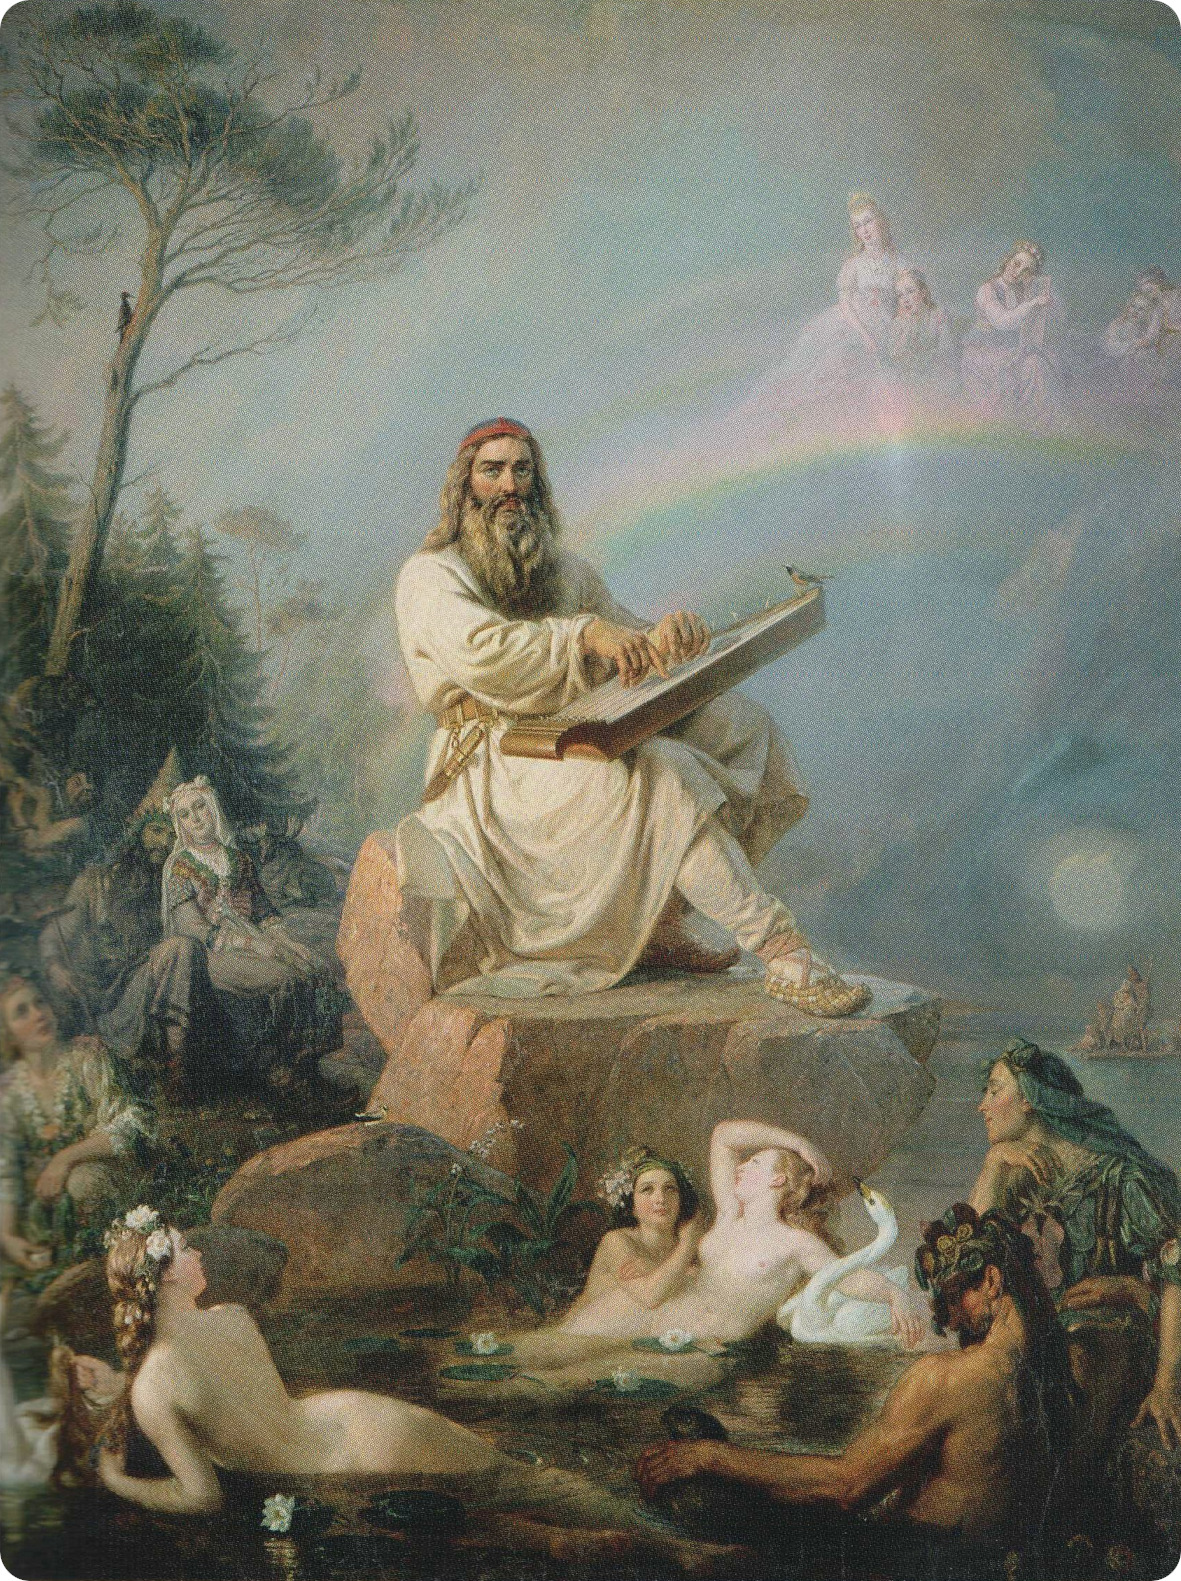
\includegraphics[width=0.82\textwidth]{Ekman_-_Vainamoisen_soitto.jpg}%
  \caption{R. W. Ekman: Väinämöisen soitto (1866)}%
\end{figure}
\vfill%


\clearpage
\subsection{Luonnon nostatus}
  \paragraph{}
  \begin{large}\begin{center}\begin{em}
    Luontoani nostattelen\\
    haastattelen haltijata\\
    Nouse luontoni lovesta\\
    Syntyni syvästä maasta\\
    Syntyni syvästä maasta\\
    \vspace{1em}
    Maasta hauna haltijani\\
    Nouse niin kuin nousit ennen\\
    Minun nostatellessani\\
    \vspace{1em}
    Isoni luonto, emoni luonto\\
    Luonto valta vanhempani\\
    Oman luontoni lisäksi\\
    Nosta Ukon voima taivahasta\\
    Maasta maan Emoisen voima\\
    \vspace{1em}
    Tuekseni turvakseni väekseni voimakseni\\
    Tulkaa tarvittaessa, käykää kutsuttaessa\\
    Terveyttä tekemään rauhaa rakentamaan\\
    \vspace{1em}
  \end{em}\end{center}\end{large}

  \paragraph{}
  %\begin{em}
    Eräs kielemme vanhimmista sanoista on ``noita'', joka on alunperin tarkoittanut tietäjää eli
    shamaania. Kristillisellä aikakaudella noita sai kielteisen kaiun. Sitä ennen tietäjät
    olivat arvokas osa yhteisöä, jonka jäseniä he tukivat sairauksissa ja elämän murroskohdissa.
    \par
    Sekä loveen lankeaminen että haltioituminen ovat tietäjien tapoja saavuttaa taianomainen
    mielentila, jossa he saavat apua esivanhemmiltaan tai suojelushengiltä.
  %\end{em}

  \paragraph{Lovi} on yliluonnollinen paikka tai olotila, aukko arkitodellisuuden ja alisen
    maailman välillä. Aliseen maailmaan kuuluu vainajala taikka Tuonela, jossa esi-isät asustavat.
    Lovi sijaitsee joko maan tai veden alla --- ilmeisesti myös naisten hameen alla, sillä
    kansanrunojen mukaan sieltäkin löytyy ovi tuonpuoleiseen. Osa muinaisista hautajaistavoistakin
    viittaa siihen, että vainaja pyrittiin palauttamaan takaisin kohtuun. Vainajalle tehtiin
    vertauskuvallisesti se, mitä sielulle toivottiin käyvän.
    \par
    Pohjolan emäntä Louhi, mahtava noita, tunnetaan myös muun muassa nimillä Lovetar ja Loviatar.
    Lovetar ilmenee syntysanoissa ja loitsun sanoissa. Louhi pystyy muuttamaan muotoaan,
    parantamaan, käskemään säätä, kuuta ja aurinkoa sekä synnyttämään mitä ihmeellisimpiä olentoja.
    Hänen kotinsa, myyttinen Pohjola, on pahojen asioiden, sairauden ja pakkasen lähde. Monet
    Pohjolan ongelmat, sairaudet ja harmit ovat itse Louhesta lähtöisin.
  \paragraph{Loveen lankeaminen:} Tietäjän matkaa vainajalaan kutsutaan loveen lankeamiseksi.
    Hurmoksessa tietäjä tekee sielunmatkan tuonpuolei\-seen ja käy kysymässä neuvoa esivanhemmilta.
    Suomalaiset tietäjät saattoivat vajota hurmokseen esimerkiksi raivoamalla, kun taas saamelainen
    \emph{noaidi} käytti apunaan rumpua. Loveen lankeamisessa käytettiin ehkä apuna myös laulamista
    [vrt. Väinämöinen laulaa Joukahaisen (Lapin tietäjän) suohon] ja soittamista (Väinämöisen
    jättihauenluinen kannel, jota kuunnelleessaan luomakunta lumoutui ja liikuttui).
    \par
    Väinämöinen lähtee Tuonelaan hakemaan puuttuvaa tietoa veneen rakentamiseen tai reen
    korjaamiseen. Joissain kertomuksissa hän hakee myös työvälineitä. Matkaa Tuonelaan
    kuvataan hyvin vaikeaksi ja vaivalloiseksi. Poiskaan sieltä ei ole helppo päästä, mutta
    Väinämöinen pakenee muuttumalla vesikäärmeeksi ja uimalla Tuonelan joen ylitse. Tämä
    viitannee muutokseen sieluneläimeksi, joiden joukossa käärmeet olivat suosittuja. Muutos
    sieluneläimeksi on yksi tietäjän keinoista.
  \paragraph{Lovesta nosto:} Loitsimalla saatetaan nostaa suvun esivanhempia eli omakuntaisia
    vainajalasta tälle puolen esimerkiksi suojelushaltijoiksi eli luonnoiksi.
  \paragraph{Luonto} on ihmisen tai muun tietoiseksi koetun olennon tai asian suojelushaltija.
    Alkuperäiseen merkitykseen viittaa ajatus jonkun luontumisesta. Luonnon katsotaann
    seuraavan ihmistä, suojelevan häntä ja tuovan hänelle onnea. Voimakasluontoiset eli ne,
    joilla on voimakas oma haltija, pärjäävät elämässä heikkoluontoisia paremmin. Luonto
    saattaa olla esimerkiksi vainajasta peräisin oleva esivanhempi eli \emph{syntyinen}.
  \paragraph{Luonnon kutsunta:} Jos ihmisellä on heikko luonto, hän saattaa joko kutsua itselleen
    vahvempaa luontoa tai voimistaa ja karaista luontoaan. Luontoa kutsutaan myös kateita,
    vihollisia ja sairauksia vastaan, ja antamaan lisää ruumiillisia, henkisiä tai yliluonnollisia
    kykyjä.
    \par
    Loitsuissa luonto nostetaan yleensä lovesta tai syvästä paikasta, vainajalasta. Joskus sitä
    kutsutaan nousemaan haon eli uppopuun alta. Joskus taas luontoa kutsutaan nousemaan ``haudan
    alta'', joka sekin viittaa siihen, että luonto on vainajalasta.
    \par
    Erään tiedon mukaan luontoaan saattaa karaista siten, että kohottaa juhlayönä järvestä hakoa
    ja kutsuu loitsulla luontoaan.
    \par
    Luontoa puhuteltaessa hänet ilmaistaan usein haltijaksi ja synnyksi. Tässä synty merkitsee
    joko myyttistä syntyä, esivanhemman sielua syntyistä tai molempia. Esimerkki loitsusta:

    \begin{center}\begin{em}
      Nouse luontoni lovesta,\\
      Syntyni syvästä maasta,\\
      Ha'on alta haltijani\\
      Vastuksia voittamah,\\
      Katehia kaatamah,\\
      Sotisia sortamahan\ldots\\
    \end{em}\end{center}

  \paragraph{Haltioituminen:} Ihmisen haltioituessa hänen luontonsa eli haltijansa hallitsee
    häntä. Tietäjät saattavat tavoitella haltioitumisen tilaa sairauksia parantaakseen tai
    muihin yliluonnollisiin tehtäviin.
    \par
    Nykyajan psykologiassa haltioituminen vertautuu lähinnä niin sanottuun flow-tilaan, jossa
    ihminen on syvästi keskittynyt tavoitteisiinsa. Joskus haltioituminen on käsitetty myös
    loveen lankeamisen vastineeksi tai taikojen harjoittamiseksi.
  \paragraph{Emuu} on olento, joka on synnyttänyt tai luonut jonkin kasvi- tai eläinlajin ---
    sen \emph{kantavanhempi} --- ja vastuussa tämän lajin toiminnasta sekä huolenpidosta.
    \par
    Metsästäjät pyytävät loitsuin kantavanhemmilta metsästysonnea. Pahaa voidaan yrittää karkottaa
    vanhempansa luo, tai uhata, että jos olento ei tottele, hänen käytöksestään kerrotaan hänen
    vanhemmalleen. Myös kantavanhempaa saatetaan käskeä panemaan lapsensa kuriin.
  \paragraph{Herättäjä} herättää ihmisen vaaran uhatessa. Jotkut väittävät omistavansa oman
    herättäjän, joka valvoo heidän untaan.
  \paragraph{Juhlia:} Nykyisistä juhlapyhistä laskiainen, helasunnuntai, juhannus, pyhäinpäivä ja 
    joulu olivat alun perin suomalaiseen alkuperäisuskontoon kuuluneita juhlia.


\subsection{Päivä, aurinko, kuu}

  \paragraph{Päivätär ja Kuutar:} Päivätär on elämää ja valoa hallitseva lämpöä ja hedelmällisyyttä
    antava hahmo. Kristillisellä kaudella hänet korvasi Neitsyt Maria. Hän on auringon ja päivän
    jumalatar, kaunis neito, jonka toveri tai kaksois\-olento on yhtä lailla kaunis kuun jumalatar
    Kuutar.
    \par
    Päivätär ja Kuutar omistavat auringon hopeaa ja kuun kultaa, joita näkyy kuun ja auringon
    hohteessa ja kultareunaisissa pilvissä auringonlaskun aikaan. Päivätär ja Kuutar näkyvät
    toisinaan Pohjolan tyttärien tavoin taivaalla kehräämässä kulta- ja hopealankaa kutoen
    siitä kultaisia ja hopeisia koruja ja vaatteita, joita neidot pyytävät kaunistuksekseen.

  \paragraph{Ilmarisen} mainitaan olleen mukana kosmisessa luomisessa, takomalla taivaankantta
    ja asettamalla taivaankappaleita.

  \begin{center}\begin{em}
    Tuli vanha Väinämöinen, ovelle asetteleikse.\\
    Sanan virkkoi, noin nimesi: ``Oi on seppo veikkoseni!\\
    Mitä paukutat pajassa, ajan kaiken kalkuttelet?''\\
    Se on seppo Ilmarinen sanan virkkoi, noin nimesi:\\
    ``Kuuta kullaista kuvoan, hope'ista aurinkoa\\
    tuonne taivahan laelle, päälle kuuen kirjokannen.''\\
  \end{em}\end{center}


\subsection{Maa}

  \paragraph{Akka} on Ukko ylijumalan nainen. Joskus hänet on tulkittu hedelmällisyyden
    jumalattareksi. Akka on luonnon naisellinen puoli, maaemonen, jonka Ukko hedelmöittää,
    ja sade saa viheriöimään. Näin saatiin aikaan maanviljelyn kannalta suotuisat ilmat.
    Akan mukaan on nimetty asteroidi \emph{8034 Akka}.
  \paragraph{Maan haltija} on nais- tai miespuolinen perhettä, taloa, satoa, karjaa ja pihapiiriä
    hoitava ja vartioiva hyvä haltija. Jos se on naispuolinen, menestyy karja hyvin, jos
    miespuolinen, menestyvät hevoset. Joskus haltijoita on pariskunta. Tällöin talo on erityisen
    onnekas.
    \par
    Haltijaa tulee kunnioittaa, niin hän hoitaa työnsä hyvin. Haltijalle on usein luvattu, että
    joka vuosi jonkun juhlan aikaan se saa osansa juhlaruuasta tai sadosta. Pyhä pihapuu on
    uhripaikka, jonka luona haltijaa kumarretaan ja sille viedään uhrilahjoja.
    \par
    Jos haltija on tavatessa hyvissä vaatteissa ja iloinen, ei hän ole onnettomuuden aiheuttaja,
    ja on vain varoittamassa. Jos haltija on pahoissa vaatteissa eikä näytä kasvojaan, on hän
    vihastunut, ja aikomassa aiheuttaa onnettomuuden. Erään perinteen mukaan tällöin on kiireesti
    mentävä paikalle, jossa haltija on näyttäytynyt, ja uhrattava alasti.
    \par
    Kun perustetaan uutta taloa, tehdään taikoja, jotta saataisiin haltija. Muuten voivat pahat
    haltijat tai maanväki asettua pihapiiriin. Erään kansanperinteen mukaan mukaan pitää polttaa
    tulta kolme päivää sillä paikalla, johon haluaa talon perustaa. Kolmantena päivänä haltija
    ilmestyy unessa. Silloin näkee, tuleeko mies- vai naishaltija vaiko pariskunta.
  \paragraph{Maahiset} eli \textbf{maanväki} ovat pieniä, ihmisenmuotoisia olentoja, jotka asuvat
    maan alla omassa maailmassaan. Usein maahisten maailma koetaan todellisen maailman
    peilikuvaksi, joka voi olla ylösalaisin.
    \par
    Maahiset voivat olla ilkikurisia. Metsässä saattaa joutua maahisten lumoihin ja eksyä
    nurinkuriseen maailmaan, jota \emph{metsänpeitoksikin} on kutsuttu. Maan väki voidaan käsittää
    myös taikavoimaksi, jota on maassa. Maanpäällisessä maailmassa maahiset ovat yleensä
    näkymättömiä. Maahisten kerrotaan myös lumoavan ihmisiä jäämään luokseen, jos ottaa vastaan
    heidän tarjoamiaan lahjoja, ruokaa tai juomaa.
  \paragraph{Sampsa Pellervoinen} kylvää maan kasvillisuuden, kaikenlaiset metsät, suot, ahot ja
    kivikotkin. Kylvö tapahtuu sammon murusten avulla. Hän on hedelmällisyyden haltija; hänet on
    rituaalisesti herätettävä joka kevät.
  \paragraph{Äkräs} on monipuolinen kasvillisuuden haltija. \emph{Loi herneet, pavut ja nauriit
    sekä antoi kaalit, pellavat ja hamput: Egres hernet Pawudh Naurit loi / Caalit Linat ia Hamput
    edestoi.}
  \paragraph{Jumi} on yliluonnollisten ilmiöiden, lähinnä panteistisen maailmanhengen nimitys.
    \emph{Marit} (volgansuomalainen kansa) viettävät vuosittain Jumolle omistettua juhlapäivää
    uhraten lihaa ja viljaa. Jumi aiheuttaa esimerkiksi eläimelle äkillisen taudin ampumalla
    näkymättömän nuolen. Arvoituksissa jumi on jokin, jolle on ominaista ehdoton paikallaanolo
    tai jota on mahdoton kiertää.

  % \subsubsection{Kivet}
    \paragraph{Kyllikki:} kivien emuu loitsuissa, joilla kiven aiheuttamia vammoja hoidetaan
  % \subsubsection{Käärme}
    \paragraph{Käres:} käärmeitten emuu
    \paragraph{Mammotar:} matojen emuu


\subsection{Meri ja vesi}

  \paragraph{Ahti:} veden jumala tai haltija
  \paragraph{Vellamo, Veen emonen, Veden emo} on hyvä ja arvostettu vedenhaltija, joka asuu veden
    alla Ahtolassa ja on Ahdin puoliso. Häntä palvotaan kalansaaliin toivossa ja purjehdussäähän
    vaikuttamaan.
    \par
    Vellamo on kaunis; hänellä on sininen lakki, kaislainen paita ja vaahtoinen vaippa.
  \paragraph{Iku-Turso} (myös \textbf{Meritursas} ja \textbf{Iku Turilas}) on vedenhaltija tai
    merihirviö, jonkinlainen alkuolento, joka on ollut olemassa maailman syntymästä lähtien.
    Runoissa se esiintyy usein Ison Tammen, maailmanpuun, kanssa.
  \paragraph{Väinämöinen}-nimen uskotaan juontuvan väinä-sanasta, joka tarkoittaa suvantoa tai
    hiljalleen virtaavaa vettä, salmea tai joensuuta. Väinämöisen lisämääreenä esiintyy myös
    \textbf{suvantolainen}.
    \par
    Väinämöinen on Ilmattaren, ilman immen ja meren poika. Hän viettää meressä kelluvan äitinsä
    kohdussa kolmekymmentä vuotta ja alkaa synnyttyään autella maailman luomisessa.
    \par
    Väinämöinen on taidokas veneenveistäjä. Hän tietää melkein kaiken tarpeellisen veneen tekoon,
    mutta ei kolmea ratkaisevan tärkeää sanaa, luotetta. Hän lähtee hakemaan niitä Tuonelasta,
    kuolleiden maasta. Väinämöinen käy myös ammoin kuolleen tietäjä Vipusen vatsassa tietoa
    hakemassa. Matka kuolleiden maahan on kuviteltu hyvin vaaralliseksi, vain mahtavien
    tietäjien on ajateltu pystyvän siihen ja tulemaan takaisin. Tässä on uistumia rituaaleista,
    joissa tietäjä vajoaa transsiin, ja hänen sielunsa liikkuu kuolleiden maailmassa suorittamassa
    tehtävää; suomalaisessa mytologiassa kerrotaan loveen lankeamisesta ja lovesta nostosta.
    \par
    Tuonen tytti toimii lautturina ja saattaa veneellään vainajat Tuonen mustan virran yli.
    Väinämöisen tytti kuitenkin huomaa olevan elossa. Väinämöinen valehtelee kuolleensa, mutta ei
    vakuuta. Tytti tietää millaisia ovat eri tavoin kuolleet: rautaan kuolleet ovat verisiä,
    hukkuneet vetisiä ja palaneet kärventyneitä. Väinämöinen kuitenkin lopulta pääsee Tuonelle.
    Tuonella hänet laitetaan nukkumaan vastenmieliseen sänkyyn tai paikkaan, joka on tehty
    käärmeistä tai täynnä käärmeitä. Hän onnistuu kuitenkin pakenemaan. Hän muuttuu vesieläimeksi,
    ja ui Tuonen joen poikki. Tuonen poika virittää rautaverkon veteen, mutta ei saa Väinämöistä
    tarttumaan. Väinämöinen palaa Tuonelta saatuaan haluamansa ja kertoo eläville Tuonelan
    oloista.
    \par
    Joissain runoissa kerrotaan, että Väinämöinen menee veneellään Rutjan koskeen, tuliseen
    pyörteeseen. Pyörre on usein tulkittu reitiksi Tuonelaan, vauhdikkaammaksi versioksi Tuonen
    joesta. Väinämöinen menee siis elävänä kuolleiden maahan. Väinämöisen veneenjäljeksi kutsutaan
    tyyntä kohtaa muuten aaltoilevalla vedenpinnalla.
    \par
    Vedenpinnan nimitysten lisäksi Väinämöiseen liittyviä nimityksiä löytyy luonnosta
    tähtitaivaalta, kuten Väinämöisen miekka tai viikate (Orion) ja Väinämöiset tai Väinämöisen
    virsut (Seulaset). Näitä tähdistöjä on käytetty suunnistamiseen vesillä. Väinämöisen
    arvellaankin alun perin liittyneen kiinteästi vesillä liikkumiseen.
    \par
    Kalevalassa Väinämöinen syntyy Ilmattaresta vanhana miehenä. Kansanrunoissa Ilmatar ei synnytä
    Väinämöistä, vaan Väinämöinen syntyy joko yksin tai Iro-neidosta.


\subsection{Ukkonen ja tuli}

    Samanistisessa kosmologiassa ihmisen maailma sijaitsee henkien asuttamien monikerroksisten ylä-
    ja alamaailmojen välissä. Joissain kansanrunoissa se kuvataan kodan pohjaksi, josta
    taivaankupoli rajaa henkien asuinsijat. Molemmissa ajatusrakennelmissa taivasta kannattaa
    maailmanpylväs ja taivaan napaa edustaa Pohjantähti.
    \par
    Käsitys sielusta kuuluu ikivanhaan pohjoiseen samanismiin. Sielun ja ruumiin pitkästä
    rinnakkaisuudesta kertoo muun muassa sukulaiskansojemme \emph{mansien} ja \emph{hantien} sana
    \emph{is}, joka on sukua suomen sanalle itse. Tähän liittyy löyly, joka sukukielissämme viittaa
    kylpemisen ohella sieluun.
  \paragraph{Ukko ylijumala} on muinainen sään ja sadon, ilman, oikeuden sekä ukkosen jumala, jota
    pyydetään avuksi esimerkiksi taisteluun tai taikuuteen ryhtyessä.
    \par
    Ukon lisänimen ``ylijumala'' voikin tulkita kahdella tapaa: joko, että hän todella on mahtavin
    (eli ylin), jumalista; tai pelkästään, että hän asuu ylhäällä taivaalla. Vahinkoa tekevän
    salamaniskun ajatellaan olevan Ukon rangaistus tai vihan ilmaus, ja elämää tuovan sateen
    hänen suopeutensa osoitus. Ukkoa muistuttava ukkosenjumala tunnettiin latvian kielessä nimellä
    \emph{Perkons} ja liettuan kielessä nimellä \emph{Perkūnas}, joista on peräisin suomen sana
    Perkele.
    \par
    Ukko iskee salamoita kirveellä, vasaralla, nuolella tai miekalla. Kokonaisen ukonilman hän saa
    aikaan puimalla riihtä, kyntäen, jyristellen vaunuillaan taivaissa, makaamalla naispuolisen
    jumaluuden kanssa, taikka kolisuttamalla konkeloa eli kelopuuta. Savukvartsia, josta
    iskettäessä syntyy kipinöitä ja palaneen hajua, nimitetään ukonkiveksi.
    \par
    Ukko kävelee pitkin askelin pilvien ja monikerroksisen taivaan yläpuolella, ja katselee
    ylhäältä maailmaa. Mahtavuudestaan huolimatta Ukko ei ole kaikkitietävä tai kaikkivaltias, vaan
    muilla henkiolennoilla ja ihmisillä on valtaa ja toimintatilaa. Ukon taivaallisessa
    valtakunnassa on heikompia henkiolentoja, joista perinteet tuntevat muun muassa päivättäret,
    kuuttaret, ilman immet, kapeet, kuumet, tuulettaret ja muita.
    \par
    Ukon kerrotaan myös pitävän pilvissä käräjiä, joten voisi olettaa, että taivaalla asuu tai
    ainakin vierailee muitakin merkittäviä henkiolentoja, joiden kanssa Ukko päättää asioista.
    Ukkoa rukoillaan pitämään käräjiä eri ongelmien voittamiseksi.

  \paragraph{Kokko} tai \textbf{vaakalintu} on jättiläismäinen kotka, sukua yleismaailmalliselle
    ukkos\-lintuhengelle, joka tunnetaan Euroopasta aina Amerikan alkuperäiskansoille asti. Se
    voi olla muistumaa ihmishahmoista jumaluutta edeltäneestä käsityksestä, jonka mukaan taivasta
    ja ukkosta hallitsee ukkoslintu. Ukkoslintuihin uskovat paitsi jotkin suomalais-ugrilaiset,
    myös monet muut kansat.
    \par
    Kokon mittasuhteet kuvataan joskus valtaviksi: toinen siipi haroo taivasta, kun toinen
    koskettaa meren luotoja.
    \par
    Kokko ja Ilmarinen osallistuvat yhä joissain tulen syntysanoissa ensimmäisen tulen iskentään,
    joka toisissa perinteissä on Ukon tehtävä. Kokko on toisinaan tarusankarien ystävä, toisinaan
    vihollinen. Joskus sen tehtävä on vartioida. Kokko kuvataan joskus rautaiseksi, joskus
    tuliseksi. Kokko pystyy kantamaan ihmistä. Se iskee tulta auttaakseen Väinämöistä polttamaan
    kasken. Myös kokon sulkia käytetään tulen iskemiseen. Joissain tulen syntykertomuksissa tuli
    on isketty kokon sulilla.
    \par
    Kokkoja voi olla useita. Eräs näistä pelastaa Väinämöisen merihädästä palkkioksi siitä, että
    kaskea kaataessaan Väinämöinen jätti koivun linnuille istumapuuksi. Ilmarinen ja Louhi tekevät
    omat kokkonsa. Ilmarinen tekee metallisen kokon, joka pyydystää suomuhauen. Louhi taas muuttuu
    itse kokoksi rakentamalla siivet ja pyrstön laivan osista ja ottamalla viikatteet
    kynsiksi.
    \par
    Sanassa vaakalintu esiintyvä ``vaaka'' tulee mahdollisesti sanasta ``vaa’as'', joka tarkoittaa
    myyttistä tulta, aaltoa ja kipua. Toinen mahdollisuus on ``vuokko'', saamelaisten kertomusten
    tietäjän apulintu.
  \paragraph{Panu} on tulen henki, auringon poika. Panuun voi vedota loitsuissa, kun ollaan
    tekemisissä tulen kanssa.


\subsection{Ilma ja tuuli}

  \paragraph{Ilmattaret} eli \textbf{Ilman immet} ovat taivaalla asuvia jumalaisia neitoja, jotka
    muistuttavat Pohjan neitoja, sillä nekin istuvat ajoittain taivaankannella.
    \par
    Ilmatar liittyy Väinämöisen ja maailman syntymään. Ilmatar tylsistyy oloonsa impenä taivaalla
    ja laskeutuu meren selälle. Tuuli hedelmöittää hänet. Sotka etsii pesäpaikkaa ja huomaa
    Ilmattaren polven, jolle se tekee pesän ja munii siihen munansa. Polvea alkaa kuumottaa ja
    Ilmatar heilauttaa sitä, jolloin munat putoavat ja särkyvät. Särkyneistä munankuorista syntyy
    maailma.
  \paragraph{Seppo Ilmarinen} on Väinölässä asuva seppäsankari, jolla on jumalallisia piirteitä.
    Häntä pidetään myös tuulen, sään ja ilman jumalana, joka on mukana maailman syntymässä.
    \par
    Iro-neito synnytti Ilmarisen yöllä ja jo päivällä Ilmarinen teki pajan. Palkeet liittyvät
    Ilmarisen asemaan tuulen jumalana, mutta toisaalta myös tämän rooliin kosmisena seppänä.
    Ilmarisen taontatyö ei onnistu ennen kuin hän tarttuu palkeisiin orjien sijasta itse.
    Ilmarinen takoi maailman alussa taivaankantta niin taidokkaasti, etteivät näy pihtien pitämät,
    eivätkä tunnu vasaran iskut. Ilmarisen kädenjälkeä ovat myös revontulet, aamu- ja iltaruskon
    värit. Myös raudan keksiminen ja alkutulen iskeminen ovat Ilmarisen saavutuksia. Ilmarinen
    takoo monia esineitä, kuten Sammon, Kultaisen naisen, ja yrittää takoa uuden Auringon ja Kuun.
    \par
    Suomalaisilla lienee ollut Ukkoa aikaisempi, omaperäinen taivaan jumala. Tämän syrjäydyttyä
    Ukon tieltä siitä kehittyi kalevalaisen perinteen seppäsankari Ilmarinen. Ilmarisen asemasta
    taivaan jumaluutena on säilynyt muistumia myytteihin, kuten uskomukset, että hän takoi
    taivaankannen ja Sammon, joka alkujaan käsitettiin taivaan tukipylvääksi.
  \paragraph{Sielulintu} on sielun koti ja vertauskuva. Lintu ehkä tuo sielun syntymässä ja vie sen
    kuoleman hetkellä. Joidenkin perinteiden mukaan nukkuessa on hyvä olla lähellä puusta
    veistetty sielulintu, joka pitää huolta sielusta unen aikana, jottei se lähtisi omille
    teilleen. Ihmisen kuoltua hänen puinen sielulintunsa laitetaan ortodoksisen hautaristin
    yläpuolelle. Lintujen ruokkiminen jouluna on vanha tapa; kuolleet eli sielulinnut ovat elävien
    kanssa mukana keskitalven juhlassa.
    \par
    Samanistisessa ihmiskuvassa sielu on usein monikerroksinen. Sen osista yksi saattaa unessa tai
    transsissa liikkua kehon ulkopuolella esimerkiksi linnun hahmossa. Lintujen merkitys
    suomalais-ugrilaisille näkyy siinäkin, että taivaan halkaisevan galaktisen vyön nimi on
    Linnunrata.
  \paragraph{Tuuletar} tarkoittaa naispuolista tuulta hallitsevaa luonnonhenkeä tai tuulen
    personoitumaa. Tuulettaria on erilaisia. Tuuletar saattaa olla yksittäinen tuulenpuuska,
    vihuri tai tuulispää, tai tietynlainen jatkuva tuuli. Tuuletar voi myös olla tuulen jumala,
    jolta pyytämällä saa suotuisaa ilmaa. Tietty tuuletar voi myös vastata tietystä ilmansuunnasta
    tulevaa tuulta.
  \paragraph{Tapiotar:} lintujen emuu


\subsection{Metsä}

  \paragraph{Tapio} on metsän haltija ja hän hallitsee metsäistä valtakuntaansa Tapiolaa. Tapion
    väki kaunistaa ja siivoaa metsää, huolehtii kasveista ja eläimistä. Tapion tyttäriä ovat
    ihastuttavat Tellervo, Tyytikki, Tuulikki ja Annikki. Tapiota ja hänen perhettään kuvaillaan
    ihmishahmoisiksi ja joko alastomiksi tai kauniisti pukeutuneiksi. Joidenkin runojen mukaan
    Tapion parta on puuta ja silmät kuin kaksi pohjatonta järveä.
  \paragraph{Mielikki} on Tapion vaimo. Metsästäjien on puheltava ja laulettava viettelevästi ja
    imartelevasti Mielikille saadakseen tältä lahjana saalista. Mielikki hoitaa metsän ``taloustyöt''
    eli siistimisen, koristelun ja kaunistamisen. Metsän kauneutta, kuten myös Mielikin omaa
    kauneutta, kannattaa metsässä liikkuessa kehua. Mielikin uskotaan lepyttävän miestään Tapiota,
    jos tämä tulee huonolle tuulelle ja usuttaa voimat metsämiehiä vastaan.
    \par
    Harvoin ihmisille näyttäytyessään Mielikki usein huvikseen pukeutuu Tapion harmaaseen
    naavaturkkiin ja -hattuun. Katsojan silmissä kuu\-sikossa kulkee höperö vanhus, joka laskee
    mättäiden marjoja.
    \par
    Mielikki on taitava parantaja. Hän hoitaa ansoihin jääneet käpälät ja tassut, pesästä pudonneet
    linnunpoikaset ja metsokukkojen taisteluhaavat. Metsän parantavat kasvit hän kerää
    huolellisesti talteen, ja niinpä hänellä on sopivia rohtoja myös ihmisten vaivoihin, jos joku
    vain keksii käydä pyytämässä. Mielikin käyttämiä kasveja ovat muun muassa kanerva ja kataja.
    \par
    Pienriistan pyytäjän, sienestäjän ja marjastajan kannattaa lausua metsään mennessään:
    \emph{``Siniviitta, viidan eukko, / mieluinen metsän e\-mäntä! / Anna tie, avaa portti / minun
    metsällä käydessäni.''} Mielikin nimi juontuu onnea ja kohtaloa merkinneestä mielu-sanasta.
  \paragraph{Tyytikki:} oravien emuu; Tapion ja hänen puolisonsa Mielikin tytär
  \paragraph{Metsän haltijat ja olennot:} Metsässä on myös arvaamattomampia tai vihamielisiä
    olentoja, kuten maahisia, metsähiisiä, menninkäisiä ja keijuja. Nämä saattavat sairastuttaa,
    eksyttää tai lumota, jos tulee näiden valtapiirille. Menninkäiset saattavat eksyttää metsässä
    kulkevan nurinkuriseen maailmaan. Metsässä saattaa olla myös noidankehä, alue, johon joutunut
    lumoutuu. Tätä saattaa merkitä esimerkiksi sienien itiöemien muodostama kehä.
    \par
    Metsän väkeä asuu muun muassa muurahaiskeoissa, puunkoloissa, kivenkoloissa, juurakoissa ja
    kannoissa. Väen taikavoimaa saattaa löytää myrskyn katkaisemien puiden murtumakohdista tai
    yhteenkasvaneista puista. Avoimella paikalla kasvava yksinäinen puu on tärkeä metsänväen
    kokoontumispaikka.
  \paragraph{Metsänneito} (myös \textbf{metsänneitsyt}, \textbf{metsänpiika}, \textbf{sinipiika})
    ilmaantuu joskus metsässä liikkuville tai yöpyville miehille: se saattaa tulla tanssimaan
    nuotiolle tai kävellä vastaan. Metsänneitsyt oli edestäpäin ihastuttavan kaunis, harsopukuinen
    ja pitkähiuksinen, mutta olennon selkäpuoli on ontto tai takaa se on vain puupökkelö. Tämän
    huomaaa kauhukseen mies, jos yrittää nähdä neidon selkäpuolen. Tällöin metsänneitsyt pelästyy
    ja lähtee.
  \paragraph{Menninkäinen} on yksinäisillä paikoilla asustava pieni ja pimeästä pitävä olento, joka
    on yleensä ihmisille suopea. Sana on ilmeisesti alun perin tarkoittanut vainajaa ja manalaista.
    Menninkäiset eivät välttämättä kestä päivänvaloa. Ne ovat vieraita ja outoja olentoja, joiden
    motiivit ovat ihmisille tuntemattomat, päin vastoin kuin tiettyihin elementteihin liittyvien
    väkien.
    \par
    Menninkäiset ovat voineet tulla mellastamaan kirkkoon öisin, jolloin niitä on pidetty pikku
    paholaisina. Ne saattavat pälyillä ihmisiä ikkunan tai puunrungon takaa, tai istuskella ryhmänä
    kivellä ihmistä tuijottaen. Menninkäiset järjestävät mielellään pitoja, joissa syödään, juodaan
    ja tanssitaan. Menninkäiset pitävät kiiltävistä esineistä.
  \paragraph{Ajattara:} paha naispuolinen olento, joka ajaa metsämiehiä ja metsästäjiä harhaan.
  \paragraph{Hongatar:} ärtyisä ja rujo karhujen emuu, honkien suojelija
  \paragraph{Juonetar:} peurojen emuu
  \paragraph{Käreitär:} kettujen emuu
  \paragraph{Laus:} porojen ja hirvien emuu
  \paragraph{Äimätär:} susien emuu


\subsection{Puut}

  \paragraph{Kati:} puiden emuu --- metsän kaunis ja nuori jumalatar, joka synnyttää puita
  \paragraph{Elämänpuu:} Nainen nähdään elämän ja kuoleman sekä niitä vastaavien ilmansuuntien
    etelän ja pohjoisen hallitsijana. Tämän äitihahmon mielikuvastoon liittyvät myös aurinko ja
    elämänpuu, joka usein mielletään koivuksi.
    \par
    Kalevalassa Iso Tammi kohoaa peittämään koko taivaankannen ja se lopulta kaadetaan. Aihelmaa
    on selitetty Linnunradan syntynä, sillä Linnunrata muistuttaa muodoltaan kaadettua puuta.
  \paragraph{Koivu:} \emph{[vesi]} suojelu, puhdistaminen. Koivunoksia on käytetty kautta aikain
    karkottamaan pahoja henkiä ihmisestä vihtomalla.
  \paragraph{Poppeli:} \emph{[vesi]} vauraus, lentäminen
  \paragraph{Haapa:} \emph{[ilma]} suojelee varkauksilta, parantaa ilmaisukykyä
  \paragraph{Mänty:} \emph{[ilma]} parantaminen, hedelmällisyys, vauraus
  \paragraph{Pihlaja:} \emph{[tuli]} psyykkiset voimat, parantaminen, voima, menestyminen, suojelu
  \paragraph{Tammi:} \emph{[tuli]} suojelu, terveys, vauraus, paraneminen, potenssi,
    hedelmällisyys, onni
  \paragraph{Saarni:} \emph{[tuli]} suojelu, terveys, mereen liittyvät rituaalit, vauraus
  \paragraph{Kataja:} \emph{[tuli]} suojelu, varkauksien esto, rakkaus, terveys


\subsection{Tieto}

  \paragraph{Antero Vipunen} on maan alla makaava vainaja tai jättiläinen; tietäjä, jolla on
    hallussaan arvokkaita ikiaikaisia loitsuja tai tietoja.
    \par
    Väinämöisen loitsusta puuttuu kolme sanaa eli luotetta. Ne saadakseen hän menee herättämään
    nukkuvan Vipusen joko hakkaamalla puut tämän haudalta tai menemällä suusta vatsaan. Vipunen
    voi myös nielaista Väinämöisen. Vatsassa Väinämöinen takoo niin kovasti, että Vipunen
    luovuttaa ja antaa sanat vatsakivusta päästäkseen.
    \par
    Viron kielessä \emph{vibu} on jousipyssy, joten Virossa Vipunen on käsitetty taitavaksi
    jousimieheksi. Useissa kertomuksen versioissa Vipusen mainitaan olevan ansastaja, kuten
    nimestä Vipunen voi päätellä. Vipusen arvellaan lainatun saamelaisista tarinoista, joissa
    käytiin noita Antereeuksen haudalla hakemassa tietoja.
  \paragraph{Väinämöinen} on taidokas loitsujen laulaja, kanteleen soittaja ja suuri tietäjä:
    \emph{``Vaka vanha Väinämöinen / Tietäjä iän ikuinen''}. Hän veistää veneen laulamalla.
    \par
    Sotajoukon laiva pysähtyy jättiläismäisen suomuhauen selkään. Hauki tapetaan, ja sen
    leukaluusta Väinämöinen tekee kanteleen. Kanteleen kielet hän saa jonkin Hiiden olennon
    hiuksista. Väinämöinen soittaa kanneltaan niin taidokkaasti, että ihmiset, eläimet ja
    jumalolennotkin tulevat kuuntelemaan, eikä ole karskeintakaan urosta, joka ei liikuttuisi
    kyyneliin.
    \par
    Eräässä yleisessä kansanrunossa Väinämöinen syntyy yöllä, tekee päivällä pajan, takoo
    rautaisen hevosen, ja ratsastaa sillä veden päällä. Joukahainen on nuori ja laiha Lapin
    tietäjä, joka kadehtii Väinämöisen laulutaitoja ja matkustaa kolme päivää haastamaan tämän
    miekan mittelöön. Väinämöinen ei suostu miekkailemaan. He loihtivat kilpaa, jonka päätteeksi
    Väinämöinen laulaa Joukahaisen suohon. Pelastautuakseen Joukahainen lupaaa Väinämöiselle
    siskonsa Ainon puolisoksi. Aino hukuttautuu, sillä hän ei halua vaimoksi vanhalle
    Väinämöiselle. Väinämöinen ratsastaa veden päällä, ja Joukahainen ampuu hänet kostoksi
    alkumereen.
    \par
    Aiemmissa runoissa Väinämöinen ja Joukahainen ovat saman äidin, Iro-neidon lapsia. He lähtevät
    yhtä matkaa kulkemaan, mutta ajautuvat erilleen ja käyvät toistensa kimppuun. Väinämöinen
    voittaa taikansa avulla. Maailmankaikkeus syntyy, kun sotka munii munansa Väinämämöisen
    polvelle Joukahaisen suistettua hänet veteen. Väinämöinen kelluu vedessä, kun vesilintu, sotka,
    pesii hänen polvelleen. Haudonta polttaa polvea, jolloin Väinämöinen vavahduttaa sitä.
    Linnun munat joutuvat mereen, hajoavat ja synnyttävät maailman. Kalevalassa sotka munii
    Väinämöistä odottavan ilmattaren polvelle, eikä Väinämöisen polvelle, kuten kansanrunoissa.
  \paragraph{Väinämöisen paluu?} Neitsyt Marjatta tulee raskaaksi puolukasta ja saa poikalapsen
    tai lapsi löytyy metsästä, jolloin etsitään turhaan myös äitiä. Väinämöinen määrää lapsen
    äpäränä suolle vietäväksi ja puulla päähän lyötäväksi. Sylilapsi alkaa puhua, syyttää
    Väinämöistä pahemmista synneistä ja huomauttaa, ettei Väinämöistäkään ole niiden takia viety
    suolle. Lapsi kastetaan Kaukomieleksi Karjalan kuninkaaksi.
    \par
    Väinämöinen suuttuu, häpeää ja poistuu vaskisella ja kuparisella veneellään, ja sanoo
    palaavansa, kun häntä tarvitaan, etsitään ja kaivataan. Samaan tapaan vesitse ja kristinuskon
    ahdistamina ovat poistuneet myös Kalevanpojat, mutta he soutivat kivellä.


\subsection{Hiisi}

  Hiisi on pyhä kulttipaikka, pyhä lehto ja mahdollisesti kalmisto. Hiideksi on myös myöhemmin
  alettu kutsua kulttipaikalla palvottua henkiolentoa, kalmiston vainajien yhteensulautuneiden
  henkien muodostamaa kollektiivia.
  \par
  Kristinuskon saapumisen jälkeen hiisi on ollut paha henkiolento ja paha paikka. Hiisistä
  muodostui kansantarinoihin pieniä pahoja tai vähintään tuhmia olentoja, joiden kotipaikka oli
  myös nimeltään Hiisi, tai joskus Hiitola. Metsähiisi ja vesihiisi olivat metsässä ja vedessä
  asuvia hiisiä, mutta myös sairauksien nimiä. Myös pyhästä hauta-alueesta tai helvetin kaltaisesta
  paikasta saatettiin puhua hiitenä. Myöhemmin hiisi-sana alkoi viitata pakanalliseen
  henkiolentoon, pienikokoiseen ilkeään haltiaan tai peikkoon.
  \par
  Kalevalassa Väinämöinen joutuu taistelemaan Lempoa, Pahaa ja Hiittä vastaan. Hiisien kotipaikka
  Hiitola sijaitsee vaikeakulkuisessa maastossa, syrjässä ihmisasutuksesta. Hiittä pahana paikkana
  on peräpohjolassa kutsuttu sanalla helsinki. Joskus hiisi rinnastetaan myös jättiläisiin tai
  vuorenpeikkoihin.
  \par
  Hiitolaan on rakennettu Hiiden linna, jossa Hiisi asuu Hiiden emännän kanssa. Hiiden emännältä
  Väinämöinen saa kanteleeseensa kielet. Hiiden linnassa asuu myös hiitolaisia --- joiden hiukset
  olivat käärmeitä --- sekä Hiiden raivoava rakki ja Hiiden kissa, Kipinätär nimeltään. Hiidellä
  on myös Hiiden ruuna, hiisien nopea hevonen ja yksi ainoa tytär, Hippe. Hipen tehtävänä on
  laittaa varkaat palauttamaan varastettu omaisuus oikeille omistajilleen. 

  \paragraph{Hiiden hirvi} on vaikeasti pyydystettävä, voimakas ja nopea hirveä muistuttava olento.
    Se saattaa olla samaa kantaa kuin samojedien ja obinugrilaisten taivaallinen peura,
    kuusijalkainen olento, jonka ensimmäinen samaani pyydysti. 


\subsection{Pohjola}

  Pohjolan emännän valtakunta kuvataan pahaksi ja kylmäksi maaksi kaukana pohjoisessa. Pohjola
  on sekä sankarien vihollinen, että pahojen asioiden, kuten pakkasen ja sairauksien, alkulähde.
  Pohjolan hyviä oloja kuitenkin kadehditaan, eivätkä kielteiset käsitykset estä kalevalaisia
  sankareita matkaamasta kohti Louhen valtakuntaa ja kosiskelemasta hänen yliluonnollisen kauniita
  tyttäriään.

  \paragraph{Pohjolan emäntä} eli \textbf{Pohjan akka} johtaa myyttistä Pohjolaa. Kalevalassa
  Pohjolan emännän nimi on \textbf{Louhi}, mutta tunnetaan muitakin nimiä: \textbf{Lovetar},
  \textbf{Loviatar}, \textbf{Louheatar} ja \textbf{Lovehetar}. Häneen viitataan säeparilla:
  \emph{``Louhi Pohjolan emäntä / Pohjan akka harvahammas''}.
  \par
  Pohjolan emännällä on suunnattomat taikavoimat: hän pystyy muuttamaan muotoaan, käskemään säätä,
  säätämään auringon ja kuun kulkua, parantamaan ja on kykeneväinen synnyttämään mitä
  ihmeellisimpiä olioita. Hän varustaa sotaveneen soutajineen ja sotaväkineen, ja veneen
  tuhouduttua ottaa veneen laidat siivikseen, ja muuntautuu jättimäiseksi Kokko-linnuksi, jonka
  selkään soturit nousevat.
  \par
  Pohjolan emäntä on synnyttänyt monia ongelmista, jotka tulevat Pohjolasta ihmisten harmiksi.
  Hänet on usein portoksi mainittu siksi, etteivät nämä ``lapset'' ole avioliitosta peräisin. Hänet
  hedelmöittää tuuli, kun hän paljastaa alapäänsä pohjoiseen päin, tai sen tekee Iku-Turso meren
  kuohuilla kovilla.
  \par
  Louhi mainitaan usein myös ihmeellisten Pohjolan neitojen äidiksi. Pohjolan isäntä jää yleensä
  sivuosaan. Yleensä miestä ei mainita ollenkaan, ja paheksuen korostetaan, että emäntä luo
  synnyttämänsä asiat ja olennot luonnottomasti ja aviottomasti.


\subsection{Sampo}

  Sampo on ihmeellinen, rikkauksia tekevä mylly: kirjokansi, ihmekone, joka jauhaa rahaa, viljaa ja
  suolaa. Sampo jauhaa, sillä maailmanpylvään on ajateltu kiertyvän taivaankannen mukana. Sillä
  arvellaan myös olevan jalat, joiden avulla se seisoo, sekä reiät tai nokat. Sammon juuret ovat
  syvällä maaemässä, ja Sammon yleinen toisintonimi on kirjokansi, joka viittaa taivaankanteen.
  Sammas on patsas, joka kannattaa taivaan kantta. Kultanappi tai kultainen naula on pohjantähti
  (tai Vega, joka oli 12 000 vuotta sitten Pohjantähden kohdalla), joka kiinnittää taivaankannen
  ja maan. Taivaankansi pyörii naulan ympäri: ``sammas jauhaa''. Myös indoeurooppalaisilla kansoilla
  on maailmanpylväsmyytti. Esimerkiksi Intiassa pylvästä kannattelee kilpikonna.
  \par
  Sampo-tarut ovat, paitsi ihmeellisiä kertomuksia kahden kansan taistelusta ja ihme-esineen
  vaiheista, alkujaan kosmisia kuvauksia. Ne selittävät maanviljelyksen syntyä ja muidenkin
  asioiden myyttistä alkuperää. Sampo on esiintynyt myös nimillä sampa, sammas, sampi, sampu,
  samppu, samppo ja sammut. Sanana sampo on sukua sammakselle eli pylväälle. Laajalti esiintyviä
  sammon piirteitä ovat hyvyys, kirjokanteen viittaus ja yhteys merelliseen Pohjolaan. Sampo
  liitetään seppien tuomaan uudenlaiseen hyvinvointiin, joka uhkaa sysäyttää Väinämöisen ja
  tietäjäkulttuurin.
  \par
  Väinämöinen lähtee Pohjolaan kosimaan Pohjolan tytärtä. Pohjolan emäntä a\-settaa kosijalle
  ehdoksi, että Väinämöisen on taottava sampo. Väinämöinen ei tähän pysty, ja hän lähtee pettyneenä
  kotiin. Hän kuitenkin lähettää sepän, Ilmarisen, takomaan Pohjolaan sammon. Seppo Ilmarinen takoo
  Sammon Pohjolan emännälle vastineeksi Pohjolan tyttärestä. Pohjolan emäntä Louhi ottaa Sammon
  vastaan, mutta kieltäytyy luovuttamasta tyttöä Ilmarisen vaimoksi. Louhi vie Sammon kivisen mäen
  sisään, juurruttaa sen maaperään, ja sulkee lukkojen taakse. Sen jälkeen sampo jauhaa rikkautta
  Pohjolan väelle. Tästä suuttuneina kalevalaiset hyökkäävät Pohjolaan ja anastavat Sammon.
  Syntyneessä taistelussa sampo tuhoutuu. Pohjan Akka saa Sammon kannen. Sammon sirpaleita
  ajelehtii kalevalaisten rantaan, ja ne saavat maanviljelyn aikaan.

  \begin{figure}[!hb]%
    \centering%
    % 0.618034^2 ~ 0.381966 (Golden Ratio)
    \includegraphics[width=.381966\textwidth]{pohjannaula_transparent_bg_525x452px.png}%
    \caption{Pohjantähti naulana liittää yhteen kuvun muotoisen taivaankannen ja sampaan eli maailmanpylvään. E. N. Setälän (1932) mukaan.}%
  \end{figure}


\subsection{Kirjallisuutta}

  \begin{itemize}
    \item Siikala, Anna-Leena: \emph{Itämerensuomalaisten mytologia}. Hämeenlinna: SKS, 2012.
    \item Siikala, Anna-Leena: \emph{Suomalainen šamanismi}. Hämeenlinna: SKS, 1992.
    \item Haavio, Martti: \emph{Suomalainen mytologia}. Porvoo Helsinki: WSOY, 1967.
    \item Ganander, Kristfried: \emph{Mythologia Fennica}. Turku: Frenckell, 1789.
    \item Emil Nestor Setälä: \emph{Sammon arvoitus: Isien runous ja usko}. Helsinki: Otava, 1932.
    \item \emph{SKVR-tietokanta}. \url{https://skvr.fi/}
  \end{itemize}

  \paragraph{}
    {\small
      Muinaissuomalaista mytologiaa ---luvun ensimmäisen version kokosi \emph{antagomir}.
    }

  \paragraph{}
    {\small
      \emph{``Nimi-instituution puuttumisesta siis johtunee, ettei vanhimmilla ihmishahmoisilla
      jumaluuksillakaan ollut erityistä nimeä, vaan naisjumaluudet olivat akkoja, jotka erotettiin
      toisistaan asuinsijojensa, tehtäviensä tai aseittensa mukaan. Toisin sanoen: akka-jumaluudet
      tuntuisivat siis olevan ajalta, jolloin uralilaiset/suomalais-ugrilaiset eivät vielä olleet
      omaksuneet kantaeuroopasta lainasanaa nimi ja siihen liittyvää nimenantoa ja proprin-käyttöä.
      Mutta akkojen aika saattoi senkin jälkeen jatkua yksinomaisena pitkään, kunnes
      kantasuomalaisten taivaalle ilmaantui kantaeurooppalainen ukkosenjumala Ilmamoinen; hän
      tarvitsi ja sai nimen. Akkojen aika kesti siten koko neljännen vuosituhannen ja suuren osan
      kolmattakin. Eivätkä akkajumalat hävinneet senkään jälkeen: Pohjan akka ja akka manteren
      alainen elivät kalevalaisessa perinteessä entiseen tapaan nimettöminä lähes nykyaikaan
      asti.''} --- Unto Salo, ``Tuoni, Pohjola, Taivas --- Arkeologian ja kalevalaisten runojen
      tuonelat (Kalevalaiset myytit ja uskomukset III)'', s. 115
    }


      \clearpage\scleardpage
      \section{Runoja, loitsuja}
        \begin{songs}{titleidx,authidx,tagidx}
          \chordsoff % songs: do not show (empty line for non-existing) chords
          % songs: increase line spacing for better readability (+.95pt is the
          % maximum so that this section doesn't extend on the next page;
          % adjust if material is added/removed):
          \baselineadj=+.95pt plus 0pt minus 0pt %
          \renewcommand{\lyricfont}{\small} % songs: use smaller font
          \songcolumns{2} % songs: two columns per page
          \songpos{1} % songs: avoid ONLY page-turns within songs
          % songs: make penalty for breaking column/page at any line of lyrics to be the same:
          % (The default for \interlinepenalty is 1000, and for all the others 200.)
          \interlinepenalty=200 %
          % Finnish spells and poems
% ========================
%
% The following sets the song number for the first song in this file.
% The number will automatically be incremented by one for each song.
% Please do not change this! Changing would make different versions of
% the songbook to have different numbers for the same songs, and it
% would totally mess up the selection booklets causing them to have
% wrong songs in them. (For the same reason, add new songs only to the
% end of each songs_ file.)
\setcounter{songnum}{700}


\beginsong{\texorpdfstring{Maailmansynty\-runo}{Maailmansyntyruno}}[by={Kalevala: 1. runo}]
  \beginverse
    Mieleni minun tekevi,
    aivoni ajattelevi
    lähteäni laulamahan,
    saa'ani sanelemahan,
    sukuvirttä suoltamahan,
    lajivirttä laulamahan.
    Sanat suussani sulavat,
    puhe'et putoelevat,
    kielelleni kerkiävät,
    hampahilleni hajoovat.
    Veli kulta, veikkoseni,
    kaunis kasvinkumppalini!
    Lähe nyt kanssa laulamahan,
    saa kera sanelemahan
    yhtehen yhyttyämme,
    kahta'alta käytyämme!
    Harvoin yhtehen yhymme,
    saamme toinen toisihimme
    näillä raukoilla rajoilla,
    poloisilla Pohjan mailla.
  \endverse
  \beginverse
    Lyökämme käsi kätehen,
    sormet sormien lomahan,
    lauloaksemme hyviä,
    parahia pannaksemme,
    kuulla noien kultaisien,
    tietä mielitehtoisien,
    nuorisossa nousevassa,
    kansassa kasuavassa:
    noita saamia sanoja,
    virsiä virittämiä
    vyöltä vanhan Väinämöisen,
    alta ahjon Ilmarisen,
    päästä kalvan Kaukomielen,
    Joukahaisen jousen tiestä,
    Pohjan peltojen periltä,
    Kalevalan kankahilta.
    Niit' ennen isoni lauloi
    kirvesvartta vuollessansa;
    niitä äitini opetti
    väätessänsä värttinätä,
    minun lasna lattialla
    eessä polven pyöriessä,
    maitopartana pahaisna,
    piimäsuuna pikkaraisna.
    Sampo ei puuttunut sanoja
    eikä Louhi luottehia:
    vanheni sanoihin sampo,
    katoi Louhi luottehisin,
    virsihin Vipunen kuoli,
    Lemminkäinen leikkilöihin.
  \endverse
  \beginverse
    Viel' on muitaki sanoja,
    ongelmoita oppimia:
    tieohesta tempomia,
    kanervoista katkomia,
    risukoista riipomia,
    vesoista vetelemiä,
    päästä heinän hieromia,
    raitiolta ratkomia,
    paimenessa käyessäni,
    lasna karjanlaitumilla,
  \endverse
  \beginverse
    metisillä mättähillä,
    kultaisilla kunnahilla,
    mustan Muurikin jälessä,
    Kimmon kirjavan keralla.
    Vilu mulle virttä virkkoi,
    sae saatteli runoja.
    Virttä toista tuulet toivat,
    meren aaltoset ajoivat.
    Linnut liitteli sanoja,
    puien latvat lausehia.
    Ne minä kerälle käärin,
    sovittelin sommelolle.
    Kerän pistin kelkkahani,
    sommelon rekoseheni;
    ve'in kelkalla kotihin,
    rekosella riihen luoksi;
    panin aitan parven päähän
    vaskisehen vakkasehen.
    Viikon on virteni vilussa,
    kauan kaihossa sijaisnut.
  \endverse
  \beginverse
    Veänkö vilusta virret,
    lapan laulut pakkasesta,
    tuon tupahan vakkaseni,
    rasian rahin nenähän,
    alle kuulun kurkihirren,
    alle kaunihin katoksen,
    aukaisen sanaisen arkun,
    virsilippahan viritän,
    kerittelen pään kerältä,
    suorin solmun sommelolta?
  \endverse
  \beginverse
    Niin laulan hyvänki virren,
    kaunihinki kalkuttelen
    ruoalta rukihiselta,
    oluelta ohraiselta.
    Kun ei tuotane olutta,
    tarittane taarivettä,
    laulan suulta laihemmalta,
    vetoselta vierettelen
    tämän iltamme iloksi,
    päivän kuulun kunniaksi,
    vaiko huomenen huviksi,
    uuen aamun alkeheksi.
    * * *
  \endverse
  \beginverse
    Noin kuulin saneltavaksi,
    tiesin virttä tehtäväksi:
    yksin meillä yöt tulevat,
    yksin päivät valkeavat;
    yksin syntyi Väinämöinen,
    ilmestyi ikirunoja
    kapehesta kantajasta,
    Ilmattaresta emosta.
  \endverse
  \beginverse
    Olipa impi, ilman tyttö,
    kave luonnotar korea.
    Piti viikoista pyhyyttä,
    iän kaiken impeyttä
    ilman pitkillä pihoilla,
    tasaisilla tanterilla.
    Ikävystyi aikojansa,
    ouostui elämätänsä,
    aina yksin ollessansa,
    impenä eläessänsä
  \endverse
  \beginverse
    ilman pitkillä pihoilla,
    avaroilla autioilla.
    Jop' on astuiksen alemma,
    laskeusi lainehille,
    meren selvälle selälle,
    ulapalle aukealle.
    Tuli suuri tuulen puuska,
    iästä vihainen ilma;
    meren kuohuille kohotti,
    lainehille laikahutti.
  \endverse
  \beginverse
    Tuuli neittä tuuitteli,
    aalto impeä ajeli
    ympäri selän sinisen,
    lakkipäien lainehien:
    tuuli tuuli kohtuiseksi,
    meri paksuksi panevi.
    Kantoi kohtua kovoa,
    vatsantäyttä vaikeata
    vuotta seitsemän satoa,
    yheksän yrön ikeä;
  \endverse
  \beginverse
    eikä synny syntyminen,
    luovu luomatoin sikiö.
    Vieri impi veen emona.
    Uipi iät, uipi lännet,
    uipi luotehet, etelät,
    uipi kaikki ilman rannat
    tuskissa tulisen synnyn,
    vatsanvaivoissa kovissa;
    eikä synny syntyminen,
    luovu luomatoin sikiö.
  \endverse
  \beginverse
    Itkeä hyryttelevi;
    sanan virkkoi, noin nimesi:
    ``Voi poloinen, päiviäni,
    lapsi kurja, kulkuani!
    Jo olen joutunut johonki:
    iäkseni ilman alle,
    tuulen tuuiteltavaksi,
    aaltojen ajeltavaksi
    näillä väljillä vesillä,
    lake'illa lainehilla!
  \endverse
  \beginverse
    Parempi olisi ollut
    ilman impenä eleä,
    kuin on nyt tätä nykyä
    vierähellä veen emona:
    vilu tääll' on ollakseni,
    vaiva värjätelläkseni,
    aalloissa asuakseni,
    veessä vierielläkseni.
    Oi Ukko, ylijumala,
    ilman kaiken kannattaja!
  \endverse
  \beginverse
    Tule tänne tarvittaissa,
    käy tänne kutsuttaessa!
    Päästä piika pintehestä,
    vaimo vatsanvääntehestä!
    Käy pian, välehen jou'u,
    välehemmin tarvitahan!''
  \endverse
  \beginverse
    Kului aikoa vähäisen,
    pirahteli pikkaraisen.
    Tuli sotka, suora lintu;
    lenteä lekuttelevi
  \endverse
  \beginverse
    etsien pesän sijoa,
    asuinmaata arvaellen.
    Lenti iät, lenti lännet,
    lenti luotehet, etelät.
    Ei löyä tiloa tuota,
    paikkoa pahintakana,
    kuhun laatisi pesänsä,
    ottaisi olosijansa.
  \endverse
  \beginverse
    Liitelevi, laatelevi;
    arvelee, ajattelevi:
  \endverse
  \beginverse
    ``Teenkö tuulehen tupani,
    aalloillen asuinsijani?
    Tuuli kaatavi tupasen,
    aalto vie asuinsijani.''
    Niin silloin ve'en emonen,
    veen emonen, ilman impi,
    nosti polvea merestä,
    lapaluuta lainehesta
    sotkalle pesän sijaksi,
    asuinmaaksi armahaksi.
  \endverse
  \beginverse
    Tuo sotka, sorea lintu,
    liiteleikse, laateleikse.
    Keksi polven veen emosen
    sinerväisellä selällä;
    luuli heinämättähäksi,
    tuoreheksi turpeheksi.
    Lentelevi, liitelevi,
    päähän polven laskeuvi.
    Siihen laativi pesänsä,
    muni kultaiset munansa:
  \endverse
  \beginverse
    kuusi kultaista munoa,
    rautamunan seitsemännen.
  \endverse
  \beginverse
    Alkoi hautoa munia,
    päätä polven lämmitellä.
    Hautoi päivän, hautoi toisen,
    hautoi kohta kolmannenki.
    Jopa tuosta veen emonen,
    veen emonen, ilman impi,
    tuntevi tulistuvaksi,
    hipiänsä hiiltyväksi;
  \endverse
  \beginverse
    luuli polvensa palavan,
    kaikki suonensa sulavan.
    Vavahutti polveansa,
    järkytti jäseniänsä:
    munat vierähti vetehen,
    meren aaltohon ajaikse;
    karskahti munat muruiksi,
    katkieli kappaleiksi.
  \endverse
  \beginverse
    Ei munat mutahan joua,
    siepalehet veen sekahan.
  \endverse
  \beginverse
    Muuttuivat murut hyviksi,
    kappalehet kaunoisiksi:
    munasen alainen puoli
    alaiseksi maaemäksi,
    munasen yläinen puoli
    yläiseksi taivahaksi;
    yläpuoli ruskeaista
    päivöseksi paistamahan,
    yläpuoli valkeaista,
    se kuuksi kumottamahan;
    mi munassa kirjavaista,
    ne tähiksi taivahalle,
    mi munassa mustukaista,
    nepä ilman pilvilöiksi.
  \endverse
  \beginverse
    Ajat eellehen menevät,
    vuoet tuota tuonnemmaksi
    uuen päivän paistaessa,
    uuen kuun kumottaessa.
    Aina uipi veen emonen,
    veen emonen, ilman impi,
  \endverse
  \beginverse
    noilla vienoilla vesillä,
    utuisilla lainehilla,
    eessänsä vesi vetelä,
    takanansa taivas selvä.
    Jo vuonna yheksäntenä,
    kymmenentenä kesänä
    nosti päätänsä merestä,
    kohottavi kokkoansa.
    Alkoi luoa luomiansa,
    saautella saamiansa
  \endverse
  \beginverse
    selvällä meren selällä,
    ulapalla aukealla.
    Kussa kättä käännähytti,
    siihen niemet siivoeli;
    kussa pohjasi jalalla,
    kalahauat kaivaeli;
    kussa ilman kuplistihe,
    siihen syöverit syventi.
  \endverse
  \beginverse
    Kylin maahan kääntelihe:
    siihen sai sileät rannat;
  \endverse
  \beginverse
    jaloin maahan kääntelihe:
    siihen loi lohiapajat;
    pä'in päätyi maata vasten:
    siihen laitteli lahelmat.
    Ui siitä ulomma maasta,
    seisattelihe selälle:
    luopi luotoja merehen,
    kasvatti salakaria
    laivan laskemasijaksi,
    merimiesten pään menoksi.
  \endverse
  \beginverse
    Jo oli saaret siivottuna,
    luotu luotoset merehen,
    ilman pielet pistettynä,
    maat ja manteret sanottu,
    kirjattu kivihin kirjat,
    veetty viivat kallioihin.
    Viel' ei synny Väinämöinen,
    ilmau ikirunoja.
    Vaka vanha Väinämöinen
    kulki äitinsä kohussa
  \endverse
  \beginverse
    kolmekymmentä keseä,
    yhen verran talviaki,
    noilla vienoilla vesillä,
    utuisilla lainehilla.
    Arvelee, ajattelevi,
    miten olla, kuin eleä
    pimeässä piilossansa,
    asunnossa ahtahassa,
    kuss' ei konsa kuuta nähnyt
    eikä päiveä havainnut.
  \endverse
  \beginverse
    Sanovi sanalla tuolla,
    lausui tuolla lausehella:
    ``Kuu, keritä, päivyt, päästä,
    otava, yhä opeta
    miestä ouoilta ovilta,
    veräjiltä vierahilta,
    näiltä pieniltä pesiltä,
    asunnoilta ahtahilta!
    Saata maalle matkamiestä,
    ilmoillen inehmon lasta,
    kuuta taivon katsomahan,
    päiveä ihoamahan,
    otavaista oppimahan,
    tähtiä tähyämähän!''
    Kun ei kuu kerittänynnä
    eikä päivyt päästänynnä,
    ouosteli aikojansa,
    tuskastui elämätänsä:
    liikahutti linnan portin
    sormella nimettömällä,
  \endverse
  \beginverse
    lukon luisen luikahutti
    vasemmalla varpahalla;
    tuli kynsin kynnykseltä,
    polvin porstuan ovelta.
    Siitä suistui suin merehen,
    käsin kääntyi lainehesen;
    jääpi mies meren varahan,
    uros aaltojen sekahan.
  \endverse
  \beginverse
    Virui siellä viisi vuotta,
    sekä viisi jotta kuusi,
  \endverse
  \beginverse
    vuotta seitsemän, kaheksan.
    Seisottui selälle viimein,
    niemelle nimettömälle,
    manterelle puuttomalle.
    Polvin maasta ponnistihe,
    käsivarsin käännältihe.
    Nousi kuuta katsomahan,
    päiveä ihoamahan,
    otavaista oppimahan,
    tähtiä tähyämähän.
  \endverse
  \beginverse
    Se oli synty Väinämöisen,
    rotu rohkean runojan
    kapehesta kantajasta,
    Ilmattaresta emosta.
  \endverse
\endsong


\beginsong{Aamulla}[tags={aamu, Aurinko}]
  \beginverse
    Terve kasvos näyttämästä,
    Päivä kulta koittamasta,
    Aurinko ylenemästä!
    Pääsit ylös altoin alta
    Yli männistön ylenit,
    Nousit kullaisna käkenä,
    Hopeaisna kyyhkyläisnä
    Tasaiselle taivahalle,
    Elollesi entiselle,
    Matkoillesi muinaisille.
  \endverse
  \beginverse
    Nouse aina aikoinasi
    Perästä tämänki päivän,
    Tuo meille tuliaisiksi
    Anna täyttä terveyttä,
    Siirrä saama saatavihin,
    Pyytö päähän peukalomme,
    Onni onkemme nenähän;
    Käy kaaresi kaunihisti,
    Päätä päivän matkuesi,
    Pääse illalla ilohon!
  \endverse
\endsong


\beginsong{Tuulen sanat}[tags={tuuli}]
  \beginverse
    Terve kuu, terve päivä,
    Terve ilma, terve tuulet,
    Pohjois- ja etelätuuli,
    Itätuuli, länsituuli
    Lapintuuli, luoetuuli
    Suvituuli, lounaistuuli,
    Päivän nousu- ja laskutuuli
    Ja kaikki väliset tuulet!
    Lepy tuuli leppeäksi
    Lauhu ilma lauhkeaksi
    Kuu kirkas kumottamahan,
    Päivä lämmin paistamahan;
    Sivu tuulet tuulekohot,
    Sivu saakohot satehet,
    Kohti kuut kumottakohot,
    Kohti päivät paistakohot!
  \endverse
\endsong


\beginsong{Löylyn sanat: terve löyly}[tags={sauna}]
  \beginverse
    Terve löyly, terve lämmin
    terve henkäys kiukainen,
    kylpy lämpimäin kivisten,
    hiki vanhan Väinämöisen.
    Löylystä vihannan vihdan,
    tervan voimasta terveiden.
  \endverse
  \beginverse
    Löyly kiukahan kivestä,
    löyly saunan sammalista.
    Tervehyttä tekemähän,
    rauhoa rakentamahan,
    kipehille voitehiksi,
    pahoille parantehiksi.
  \endverse
\endsong


\beginsong{Löylyn sanat: tule löylyhyn}[tags={sauna}]
  \musicnote{Melodia: Kalevala-sävelmä tai esim. Hedingarna: Täss' on nainen}
  \beginverse
    Tule löylyhyn, Jumala,
    Iso ilman, lämpimähän,
    Terveyttä tekemähän,
    Rauhoa rakentamahan
  \endverse
  \beginverse
    Lyötä maahan liika löyly
    Paha löyly pois lähetä
    Ettei polta tyttöjäsi
    Turmele tekemiäsi
  \endverse
  \beginverse
    Minkä vettä viskaelen
    Noille kuumille kivillen
    Se medeksi muuttukohon
    Simaksi sirahtakohon
  \endverse
  \beginverse
    Juoskohon joki metinen
    Simalampi laikkukohon
    Läpi kiukahan kivisen
    Läpi saunan sammalisen!
  \endverse
\endsong


\beginsong{Ihmisen synty}[]
  \beginverse
    Ihminen ihala ilme,
    Sukukunnan suuri luomus,
    Tehty on mullan kakkarasta,
    Mullan kaakusta rakettu,
    (Sille Herra hengen antoi,
    Luoja suustahan sukesi.)
  \endverse
\endsong


\beginsong{Karhun synty}[]
  \beginverse
    Otsoseni, ainoiseni,
    Mesikämmen kaunoiseni,
    Kyllä mä sukusi tieän,
    Miss' oot otso syntynynnä,
    Saatuna sinisaparo,
    Jalka kyntinen kyhätty:
    Tuoll' oot otso syntynynnä
    Ylähällä taivosessa,
    Kuun kukuilla, päällä päivän,
    Seitsentähtien selällä,
    Ilman impien tykönä,
    Luona luonnon tyttärien.
  \endverse
  \beginverse
    Tuli läikkyi taivahasta,
    Ilma kääntyi kehrän päällä,
    Otsoa suettaessa,
    Mesikkiä luotaessa.
    Sieltä maahan laskettihin
    Vierehen metisen viian,
    Hongattaren huolitella,
    Tuomettaren tuu'itella,
    Juurella nyrynärehen,
    Alla haavan haaralatvan,
    Metsän linnan liepehellä,
    Korven kultaisen kotona.
  \endverse
  \beginverse
    Siitä otso ristittihin,
    Karvahalli kastettihin,
    Metisellä mättähällä,
    Sarajoen salmen suulla,
    Pohjan tyttären sylissä.
    Siinä se valansa vannoi
    Pohjan eukon polven päässä,
    Essä julkisen Jumalan,
    Alla parran autuahan,
    Tehä ei syytä syyttömälle,
    Vikoa viattomalle,
    Käyä kesät kaunihisti,
    Soreasti sorkutella,
    Elellä ajat iloiset
    Suon selillä, maan navoilla,
    Kilokangasten perillä;
    Käyä kengättä kesällä,
    Sykysyllä syylingittä,
    Asua ajat pahemmat,
    Talvikylmät kyhmästellä,
    Tammisen tuvan sisässä,
    Havulinna liepehellä,
    Kengällä komean kuusen,
    Katajikon kainalossa.
  \endverse
\endsong


\beginsong{Kiven synty}[]
  \beginverse
    Ken kiven kiveksi tiesi,
    Kun oli otraisna jyvänä,
    Nousi maasta mansikkana,
    Puun juuresta puolukkana,
    Taikka häilyi hattarassa,
    Piili pilvien sisässä,
    Tuli maahan taivahasta,
    Putosi punakeränä,
    Kaaloi kakraisna kapuna,
    Vieri vehnäisnä mykynä,
    Läpi pilvipatsahien,
    Puhki kaarien punaisten,
    Hullu huutavi kiveksi,
    Maan munaksi mainitsevi.
  \endverse
\endsong


\beginsong{Noidan synty}[]
  \beginverse
    Kyllä tieän noian synnyn,
    Sekä alun arpojia:
    Tuoll' on noita syntynynnä,
    Tuolla alku arpojien,
    Pohjan penkeren takana,
    Lapin maassa laakeassa;
    Siell' on noita syntynynnä,
    Siellä arpoja sikesi,
    Hakoisella vuotehella,
    Kivisellä pääalalla.
  \endverse
\endsong


\beginsong{Puiden synty}[]
  \beginverse
    Sampsa poika Pellervoinen
    Kesät kentällä makasi
    Keskellä jyväketoa,
    Jyväparkan parmahalla;
    Otti kuusia jyviä,
    Seitsemiä siemeniä,
    Yhen nää'än nahkasehen,
    Koipehen kesäoravan,
    Läksi maita kylvämähän,
    Toukoja tihittämähän.
  \endverse
  \beginverse
    Kylvi maita kyyhätteli,
    Kylvi maita, kylvi soita,
    Kylvi auhtoja ahoja,
    Panettavi paasikoita.
    Kylvi kummut kuusikoiksi,
    Mäet kylvi männiköiksi,
    Kankahat kanervikoiksi,
    Notkont nuoriksi vesoiksi.
    Noromaille koivut kylvi,
    Lepät maille leyhkeille,
    Kylvi tuomet tuorehille,
    Pihlajat pyhille maille,
    Pajut maille paisuville,
    Raiat nurmien rajoille,
    Katajat karuille maille,
    Tammet virran vierimaille.
  \endverse
  \beginverse
    Läksi puut ylenemähän,
    Vesat nuoret nousemahan,
    Tuuliaisen tuu'ittaissa,
    Ahavaisen liekuttaissa,
    Kasvoi kuuset kukkalatvat,
    Lautui lakkapäät petäjät,
    Nousi koivuset noroilla,
    Lepät mailla leyhkeillä,
    Tuomet mailla tuorehilla,
    Pihlajat pyhillä mailla,
    Pajut mailla paisuvilla,
    Raiat mailla raikkahilla,
    Katajat karuilla mailla,
    Tammet virran vieremillä.
  \endverse
\endsong


\beginsong{Tammen synty}[]
  \beginverse
    Oli ennen neljä neittä,
    Kolme kuulua tytärtä,
    Sininurmen niitännässä,
    Korttehen kokoannassa,
    Nenässä utuisen niemen,
    Päässä saaren terhenisen.
    Niitit päivän, niitit toisen,
    Niitit kohta kolmannenki,
    Minkä niitit, sen haravoit,
    Kaikki karhille vetelit,
    Laitit heinät lallosille,
    Sataisille saprasille,
    Siitä suovahan kokosit,
    Saatoit sankapieleksihin.
  \endverse
  \beginverse
    Jo oli nurmi niitettynä,
    Heinät luotu pielin pystyin,
    Tuli Turjan lappalainen,
    Nimeltä tulinen Tursas,
    Tunki heinäset tulehen,
    Paiskasi panun väkehen.
  \endverse
  \beginverse
    Tuli tuhkia vähäinen,
    Kypeniä pikkarainen,
    Tytöt tuossa arvelevat,
    Neiet neuvoa pitävät,
    Kunne tuhkat koottanehen,
    Poron pohjat pantanehen:
    ``Noistapa puuttuvi poroa,
    Lipeätä liuvahtavi,
    Pestä päätä Päivän poian,
    Silmiä hyvän urohon''.
  \endverse
  \beginverse
    Tuli tuuli tunturista,
    Kova ilma koillisesta,
    Tuonne tuuli tuhkat kantoi,
    Porot koillinen kokosi,
    Nenästä utuisen niemen,
    Päästä saaren terhenisen,
    Korvalle tulisen kosken,
    Pyhän virran vieremille.
    Tuuli tuopi tammen terhon,
    Kantoi maalta kaukaiselta
    Korvalle tulisen kosken,
    Pyhän virran vieremille,
    Heitti paikalle hyvälle,
    Maan lihavan liepehelle.
    Nousi tuosta nuori taimi,
    Vesa verraton vetihe,
    Siitä kasvoi kaunis tammi,
    Yleni rutimon raita,
    Latva täytti taivahille,
    Oksat ilmoille olotti.
  \endverse
\endsong


\beginsong{Tulen synty}[tags={tuli}]
  \beginverse
    Ei tuli syviltä synny,
    Eikä kasva karkealta,
    Tuli syntyi taivosessa,
    Seitsentähtyen selällä,
    Siell' on tulta tuu'iteltu,
    Valkeaista vaapoteltu,
    Kultaisessa kursikossa,
    Kultakunnahan kukulla.
  \endverse
  \beginverse
    Kasi kaunis, neito nuori,
    Tulityttö taivahinen,
    Tuopa tulta tuu'ittavi,
    Vaapottavi valkeata,
    Tuolla taivahan navoilla,
    Yllä taivahan yheksän,
    Hopeaiset nuorat notkui,
    Koukku kultainen kulisi,
    Neien tulta tuu'ittaissa,
    Vaapottaissa valkeaista.
  \endverse
  \beginverse
    Putosi tuli punainen,
    Kirposi kipuna yksi,
    Kultaisesta kursikosta,
    Hopeaisesta sulusta,
    Ilmalta yheksänneltä,
    Kaheksannen kannen päältä,
    Läpi taivahan tasaisen,
    Halki tuon ihalan ilman,
    Läpi ramppalan ovista,
    Läpi lapsen vuotehesta;
    Paloi polvet poikuelta,
    Paloi paarmahat emolta.
  \endverse
  \beginverse
    Se lapsi meni manalle,
    Katopoika tuonelahan,
    Kun oli luotu kuolemahan,
    Katsottu katoamahan,
    Tuskissa tulen punaisen,
    Angervoisen ailuissa;
    Märäten meni manalle,
    Torkahellen tuonelahan,
    Tuonen tyttöjen torua,
    Manan lasten lausuella.
  \endverse
  \beginverse
    Emopa ei manalle mennyt;
    Akka oli viisas villikerta,
    Se tunsi tulen lumoa,
    Valkeaisen vaivutella,
    Läpi pienen neulan silmän,
    Halki kirvehen hamaran,
    Puhki kuuman tuuran putken,
    Kerivi tulen kerälle,
    Suorittavi sommelolle,
    Kierähyttävi keräsen
    Pitkin pellon pientaretta,
    Läpi maan, läpi manuen,
    Työnti Tuonelan jokehen,
    Manalan syväntehesen.
  \endverse
\endsong

%% % Tulen synty, toinen versio
%%\beginsong{Tulen synty B}[tags={tuli}]
%%  \beginverse
%%    Tulta iski ilman Ukko,
%%    Valahutti valkeata,
%%    Miekalla tuliterällä
%%    Säilällä säkenevällä,
%%    Ylisessä taivosessa,
%%    Tähtitarhojen takana.
%%  \endverse
%%  \beginverse
%%    Saipa tulta iskemällä,
%%    Kätkevi tulikipunan
%%    Kultaisehen kukkarohon,
%%    Hopeaisehen kehä'än,
%%    Antoi neien tuu'itella,
%%    Ilman immen vaapotella.
%%  \endverse
%%  \beginverse
%%    Neiti pitkän pilven päällä,
%%    Impi ilman partahalla,
%%    Tuota tulta tuu'ittavi,
%%    Valkeaista vaapottavi,
%%    Kultaisessa kätkyessä,
%%    Hihnoissa hopeisissa;
%%    Hopeiset hihnat helkkyi,
%%    Kätkyt kultainen kulisi,
%%    Pilvet liikkui, taivot naukui,
%%    Taivon kannet kallistihe,
%%    Tulta tuu'iteltaessa,
%%    Valkeata vaapottaissa.
%%  \endverse
%%  \beginverse
%%    Impi tulta tuu'itteli,
%%    Valkeaista vaapotteli,
%%    Tulta sormin suoritteli,
%%    Käsin vaali valkeaista,
%%    Tuli tuhmalta putosi,
%%    Valkea varattomalta,
%%    Kätösistä käänteliän,
%%    Sormilta somittelian.
%%  \endverse
%%  \beginverse
%%    Kirposi tulikipuna,
%%    Suikahti punasoronen,
%%    Läpi läikkyi taivosista,
%%    Puhki pilvistä putosi.
%%    Päältä taivahan yheksän,
%%    Halku kuuen kirjokannen.
%%  \endverse
%%  \beginverse
%%    Tuikahti tulikipuna,
%%    Putosi punasoronen,
%%    Luojan luomilta tiloilta,
%%    Ukon ilman iskemiltä,
%%    Puhki reppänän retuisen,
%%    Kautta kuivan kurkihirren,
%%    Tuurin uutehen tupahan,
%%    Palvosen laettomahan;
%%    Sitten sinne tultuansa
%%    Tuurin uutehen tupahan,
%%    Panihe pahoille töille,
%%    Löihe töille törkeille:
%%    Riipi rinnat tyttäriltä,
%%    Käsivarret neitosilta,
%%    Turmeli pojilta polvet,
%%    Isännältä parran poltti.
%%  \endverse
%%  \beginverse
%%    Äiti lastansa imetti
%%    Kätkyessä vaivaisessa
%%    Alla reppänän retuisen;
%%    Siihen tultua tulonen
%%    Poltti lapsen kätkyestä,
%%    Puhki paarmahat emolta,
%%    Meni siitä mennessänsä,
%%    Vieri vieriellessänsä,
%%    Ensin poltti paljon maita,
%%    Paljon maita, paljon soita,
%%    Poltti auhtoja ahoja,
%%    Sekä korpia kovasti,
%%    Viimein vieprahti vetehen,
%%    Aaltoihin Aluejärven.
%%  \endverse
%%  \beginverse
%%    Tuosta tuo Aluejärvi
%%    Oli syttyä tulehen,
%%    Säkehinä säihkyellä,
%%    Tuon tuiman tulen käsissä,
%%    Ärtyi päälle äyrästensä,
%%    Kuohui päälle korpikuusten,
%%    Kuohui kuiville kalansa,
%%    Arinoille ahvenensa.
%%  \endverse
%%  \beginverse
%%    Viel' ei viihtynyt tulonen,
%%    Aalloista Aluejärven,
%%    Karkasi katajikkohon,
%%    Niin paloi katajakangas,
%%    Kohahutti kuusikkohon,
%%    Poltti kuusikon komean,
%%    Vieri vieläki etemmä,
%%    Poltti puolen Pohjanmaata,
%%    Sakaran Savon rajoa,
%%    Kappalehen Karjalata.
%%  \endverse
%%  \beginverse
%%    Kävi siitä kätkösehen,
%%    Pillojansa piilemähän,
%%    Heittihe lepeämähän
%%    Kahen kannon juuren alle,
%%    Lahokannon kainalohon,
%%    Leppäpökkelön povehen,
%%    Sieltä tuotihin tupihin,
%%    Honkaisihin huonehisin,
%%    Päivällä käsin pi'ellä
%%    Kivisessä kiukahassa,
%%    Yöllä lie'essä levätä
%%    Hiilisessä hinkalossa.
%%  \endverse
%%\endsong


\beginsong{Veden synty}[tags={vesi}]
  \beginverse
    Tiettävä on vetosen synty,
    Kanssa kastehen sijentö:
    Vesi on tullut taivosesta,
    Pilvistä pisarehina,
    Siitä vuoressa sikesi,
    Kasvoi kallion lomassa.
    Vesiviitta Vaitan poika,
    Suoviitta Kalevan poika,
    Veen kaivoi kalliosta,
    Veen vuoresta valutti,
    Kepillänsä kultaisella,
    Sauvallansa vaskisella.
  \endverse
  \beginverse
    Vuoresta valuttuansa,
    Kalliosta saatuansa,
    Vesi heilui hettehenä,
    Kulki pieninä puroina,
    Siitä suureksi sukeni,
    Sai jokena juoksemahan,
    Virtana vipajamahan,
    Koskena kohajamahan,
    Tuonne suurehen merehen,
    Alaisehen aukehesen.
  \endverse
\endsong


\beginsong{Raudan synty}[]
  \beginverse
    Itse ilmoinen Jumala,
    Tuo Ukko, ylinen Luoja,
    Hieroi kahta kämmentänsä
    Vasemmassa polven päässä,
    Siitä syntyi neittä kolme,
    Koko kolme Luonnotarta,
    Rauan ruostehen emoiksi,
    Suu sinervän siittäjiksi.
  \endverse
  \beginverse
    Neiet käyä notkutteli,
    Astui immet ilman äärtä,
    Utarilla uhkuvilla,
    Nännillä pakottavilla,
    Lypsit maalle maitojansa,
    Uhkutit utariansa,
    Lypsit maille, lypsit soille,
    Lypsit vienoille vesille.
    Yksi lypsi mustan maion,
    Vanhimpainen neitoksia,
    Toinen puikutti punaisen,
    Keskimmäinen neitosia,
    Kolmas valkean valutti,
    Nuorimpainen neitosia.
    Ku on lypsi mustan maion,
    Siitä syntyi melto rauta,
    Ku on puikutti punaisen,
    Siit' on saatu rääkyrauta,
    Ku on valkean valutti,
    Siit' on tehtynä teräkset.
  \endverse
  \beginverse
    Oli aikoa vähäisen,
    Rauta tahtovi tavata
    Vanhempata veljeänsä,
    Käyä tulta tuntemassa.
    Tuli tuhmaksi repesi,
    Kovin kasvoi kauheaksi,
    Poltti soita, poltti maita,
    Poltti korpia kovia,
    Oli polttoa poloisen
    Rauta raukan veikkosensa;
    Rauta pääsevi pakohon,
    Pakohon ja piilemähän
    Pimeähän Pohjolahan,
    Lapin laajalle perälle,
    Suurimmalle suon selälle,
    Tuiman tunturin laelle,
    Jossa joutsenet munivat,
    Hanhi poiat hautelevi.
  \endverse
  \beginverse
    Rauta suossa soikottavi,
    Vetelässä vellottavi,
    Piili vuoen, piili toisen,
    Piili kohta kolmannenki,
    Ei toki pakohon pääsnyt
    Tulen tuimista käsistä,
    Piti käyä toisen kerran,
    Lähteä tulen tuville,
    Astalaksi tehtäessä,
    Miekaksi taottaessa.
  \endverse
  \beginverse
    Susi juoksi suota myöten,
    Karhu kangasta samosi,
    Suo nousi suen jaloissa,
    Kangas karhun kämmenissä,
    Kasvoi rautaiset karangot,
    Teräksiset tierottimet,
    Suen sorkkien sijoille,
    Karhun kannan kaivamille.
  \endverse
  \beginverse
    Tuop' on seppo Ilmarinen,
    Taki taitava takoja,
    Oli teitensä käviä,
    Matkojensa mitteliä,
    Joutuvi suen jälille,
    Karhun kantapään sijoille.
    Näki rautaiset orahat,
    Teräksiset tierottimet,
    Suen suurilla jälillä,
    Karhun kannan kääntämillä,
    Sanovi sanalla tuolla:
    ``Voi sinua rauta raukka,
    Kun olet kurjassa tilassa,
    Alahaisessa asussa,
    Suolla sorkissa sutosen,
    Aina karhun askelissa',
    Kasvaisitko kaunihiksi,
    Koreaksi korkenisit,
    jos sun suosta suorittaisin,
    Sekä saattaisin pajahan,
    Tunkisin tulisijahan,
    Ahjohon asettelisin?''
  \endverse
  \beginverse
    Rauta raukka säpsähtihe,
    säpsähtihe, säikähtihe,
    Kun kuuli tulen sanomat,
    Tulen tuiman maininnaiset.
  \endverse
  \beginverse
    Sanoi seppo Ilmarinen:
    ``Et sä synny rauta raukka,
    Ei sinun suku sukeu,
    Eikä kasva heimokunta,
    Ilman tuimatta tuletta,
    Ilman viemättä pajahan,
    Ahjohon asettamatta,
    Lietsimellä lietsomatta;
    Vaan ellös sitä varatko,
    Ellös olko milläskänä,
    Tuli ei polta tuttuansa,
    Herjaele heimoansa;
    Kun tulet tulen tuville,
    Hiilisehen hinkalohon,
    Siellä kasvat kaunihiksi,
    Ylenet ylen ehoksi,
    Miesten miekoiksi hyviksi,
    Naisten nauhan päättimiksi.''
  \endverse
  \beginverse
    Senpä päivyen perästä
    Rauta suosta sotkettihin,
    Vetelästä vellottihin,
    Saatihin saven seasta;
    Itse seppo suossa seisoin
    Polvin mustassa murassa
    Rauan suosta raaettaissa,
    Maan murasta muokattaissa,
    Otti rautaiset orahat,
    Teräksiset tierottimet,
    Suen suurista jälistä,
    Karhun kantapään tiloista.
  \endverse
  \beginverse
    Se on seppo Ilmarinen
    Siihen painoi palkehensa,
    Siihen ahjonsa asetti,
    Suurille suen jälille,
    Karhun kannan hiertimille;
    Rauan tunkevi tulehen,
    Lietsoi yön levähtämättä,
    Päivän umpehuttamatta,
    Lietsoi päivän, lietsoi toisen,
    Lietsoi kohta kolmannenki,
    Rauta vellinä venyvi,
    Kuonana kohaelevi,
    Venyi vehnäisnä tahasna,
    Rukihisna taikinana,
    Sepon suurissa tulissa,
    Ilmi valkean väessä.
  \endverse
  \beginverse
    Siitä seppo Ilmarinen
    Katsoi ahjonsa alusta,
    Mitä ahjo antanevi,
    Palkehensa painanevi.
    Ensin saapi rääkyrauan,
    Sitten kuonaisen kuletti,
    Siitä valkean valutti
    Alisesta lietsimestä.
  \endverse
  \beginverse
    Siinä huuti rauta raukka:
    ``Oi sie seppo Ilmarinen
    Ota pois minua täältä
    Tuskista tulen vihaisen!''
  \endverse
  \beginverse
    Sanoi seppo Ilmarinen:
    ``Jos otan sinun tulesta,
    Ehkä kasvat kauheaksi,
    Kovin raivoksi rupeat,
    Vielä veistät veljeäsi,
    Lastuat emosi lasta.''
  \endverse
  \beginverse
    Siinä vannoi rauta raukka,
    Vannoi vaikean valansa,
    Ahjossa, alaisimella,
    Vasaroilla valkkamilla:
    ``En mä liikuta lihoa,
    Enkä verta vierehytä;
    On mun puuta purrakseni,
    Haukatakseni hakoa,
    Närettä näpätäkseni,
    Kiven syäntä syöäkseni,
    Ett' en veistä veljeäni,
    Lastua emoni lasta.
    Parempi on ollakseni,
    Ehompi eleäkseni,
    Kulkialla kumppalina,
    Käyvällä käsiasenna,
    Kuin sukua suin piellä,
    Heimoani herjaella.''
  \endverse
  \beginverse
    Silloin seppo Ilmarinen,
    Takoja ijän ikuinen,
    Rauan tempasi tulesta,
    Asetti alaisimelle,
    Rakentoa raukeaksi,
    Takoa teräkaluiksi,
    Keihä'iksi, kirvehiksi,
    Kaikenlaisiksi kaluiksi.
    Takoa taputtelevi,
    Lyöä helkähyttelevi,
    Vaan ei kiehu rauan kieli,
    Ei sukeu suu teräksen,
    Rauta ei kasva karkeaksi,
    Terä rauan tenhosaksi.
  \endverse
  \beginverse
    Siitä seppo Ilmarinen
    Arvellen ajatelevi,
    Mitä tuohon tuotanehen
    Ja kuta ve'ettänehen
    Teräksen tekomujuiksi,
    Rauan karkaisuvesiksi.
    Laati pikkuisen poroa,
    Lipeäistä liuvotteli,
    Siitä koitti kielellänsä,
    Hyvin maistoi mielellänsä,
    Itse tuon sanoiksi virkki:
    ``Ei nämät hyvät minulle
    Teräksen tekovesiksi,
    Rautojen rakento-maiksi.''
  \endverse
  \beginverse
    Mehiläinen maasta nousi
    Sinisiipi mättähästä,
    Lentelevi, liitelevi,
    Ympäri sepon pajoa;
    Senp' on seppo Ilmarinen
    Käski käyä metsolassa,
    Tuoa mettä metsolasta,
    Simoa simasalosta,
    Teräksille tehtäville,
    Rauoille rakettaville.
  \endverse
  \beginverse
    Herhiläionen Hiien lintu,
    Hiien lintu, Lemmon katti,
    Lensi ympäri pajoa
    Kipujansa kaupotellen,
    Lentelevi, kuuntelevi
    Sepon selviä sanoja
    teräksistä tehtävistä,
    Rauoista rakettavista.
  \endverse
  \beginverse
    Tuo oli siiviltä sivakka,
    Kynäluilta luikkahampi,
    Tuop' on ennätti e'ellä,
    Nouti Hiien hirmuloita,
    Kantoi käärmehen kähyjä,
    Maon mustia mujuja,
    Kusiaisen kutkelmoita,
    Sammakon salavihoja,
    Teräksen tekomujuihin,
    Rauan karkaisuvetehen.
  \endverse
  \beginverse
    Itse seppo Ilmarinen,
    Takoja alinomainen,
    Luulevi, ajattelevi,
    Mehiläisen tulleheksi,
    Tuon on mettä tuoneheksi,
    Kantaneheksi simoa,
    Sanan virkkoi, noin nimesi:
    ``Kas nämät hyvät minulle
    Teräksen tekovesiksi,
    Rautojen rakennusmaiksi.''
    Siihen kasti rauta raukan,
    Siihen tempaisi teräksen,
    Pois tulesta tuotaessa,
    Ahjosta otettaessa;
    Siitä sai teräs pahaksi,
    Rauta raivoksi rupesi,
    Veisti raukka veljeänsä,
    Sukuansa suin piteli,
    Veren laski vuotamahan,
    Hurmehen hurajamahan.
  \endverse
\endsong


\beginsong{Varjele vakainen luoja}[by={Kalevala: 43. runo}]
  \beginverse
    Anna Luoja, suo Jumala
    Anna onni ollaksemme.
    Hyvin ain’ eleäksemme,
    Kunnialla kuollaksemme.
    Suloisessa Suomenmaassa
    Kaunihissa Karjalassa!
  \endverse
  \beginverse
    Varjele, vakainen Luoja
    Kaitse, kaunoinen Jumala,
    Ole puolla poikiesi,
    Aina lastesi apuna,
    Aina yöllisnä tukena,
    Päivällisnä vartiana.
  \endverse
\endsong


% \sclearpage
% \beginsong{Höyhensaaret}[by={Eino Leino}]
%   \beginverse
%     Mitä siitä jos nuorna ma murrunkin
%     tai taitun ma talvisäihin,
%     moni murtunut onpi jo ennemmin
%     ja jäätynyt elämän jäihin.
%     Kuka vanhana vaappua tahtoiskaan?
%     Ikinuori on nuoruus laulujen vaan
%     ja kerkät lemmen ja keväimen,
%     ilot sammuvi ihmisten.
%   \endverse
%   \beginverse
%     Mitä siitä jos en minä sammukaan
%     kuin rauhainen, riutuva liesi,
%     jos sammun kuin sammuvat tähdet vaan
%     ja vaipuvi merillä miesi.
%     Kas, laulaja tähtiä laulelee
%     ja hän meriä suuria seilailee
%     ja hukkuvi hyrskyhyn, ennen kuin
%     käy purjehin reivatuin.
%   \endverse
%   \beginverse
%     Mitä siitä jos en minä saanutkaan,
%     mitä toivoin ma elämältä,
%     kun sain minä toivehet suuret vaan
%     ja kaihojen kantelen hältä.
%     Ja vaikka ma laps olen pieni vain,
%     niin jumalten riemut ma juoda sain
%     ja juoda ne täysin siemauksin ---
%     niin riemut kuin murheetkin.
%   \endverse
%   \beginverse
%     Ja vaikka ma laps olen syksyn vaan
%     ja istuja pitkän illan,
%     sain soittaa ma kielillä kukkivan maan
%     ja hieprukan hivuksilla.
%     Niin mustat, niin mustat ne olivat;
%     ja suurina surut ne tulivat,
%     mut kaikuos riemu nyt kantelen
%     vielä kertasi viimeisen!
%   \endverse
%   \beginverse
%     Oi, kantelo pitkien kaihojen,
%     sinä aarteeni omani, ainoo!
%     Me kaksi, me kuulumme yhtehen,
%     jos kuin mua kohtalot vainoo.
%     Me kuljemme kylästä kylähän näin,
%     ohi kylien koirien räkyttäväin,
%     ja keskellä raition raakuuden
%     sävel soipa on keväimen.
%   \endverse
%   \beginverse
%     Me kaksi, me tulemme metsästä
%     ja me metsien ilmaa tuomme,
%     me laulamme nuoresta lemmestä
%     ja lempemme kuvan me luomme,
%     me luomme sen maailman tomusta niin
%     kuin Luoja loi ihmisen Eedeniin
%     ja korvesta kohoitamme me sen
%     kun vaskisen käärmehen.
%   \endverse
%   \beginverse
%     Te ystävät, joiden rinnassa kyyt
%     yön-pitkät pistää ja kalvaa,
%     te, joita jäytävi sydämen syyt
%     ja elämä harmaja halvaa,
%     oi, helise heille mun kantelein,
%     oi, helise onnea haavehein
%     ja unta silmihin unettomiin
%     mun silmäni suljit sa niin.
%     Kas, ylläpä mustien murheiden
%     on kaunihit taivaankaaret
%     ja kaukana keskellä aaltojen
%     on haaveiden höyhensaaret
%     ja ken sinne lapsosen kaarnalla käy,
%     ei sille ne aavehet yölliset näy,
%     vaan rinnoin hän uinuvi rauhaisin
%     kuin äitinsä helmoihin.
%   \endverse
%   \beginverse
%     Mitä siitä jos valhetta onkin ne vaan
%     ja kestä ei päivän terää!
%     Me uinumme siksi kuin valveutaan
%     ja vaivat ne jällehen herää.
%     Moni nukkui nuorihin toiveisiin
%     ja heräsi hapsihin hopeisiin;
%     hän katsahti ympäri kummissaan
%     ja --- uinahti uudestaan.
%     Miks ihmiset tahtoa, taistella
%     ja koittaa korkealle?
%     Me olemme kaikki vain lapsia
%     ja murrumme murheen alle.
%     Miks emme me kaikki vois uinahtaa
%     ja hyviä olla ja hymytä vaan
%     ja katsoa katsehin kirkkahin
%     vain sielumme syvyyksiin?
%   \endverse
%   \beginverse
%     Oi, unessa murheet ne unhottuu
%     ja rauhaton rauhan saapi,
%     oi, unessa vankikin vapautuu,
%     sen kahlehet katkeaapi,
%     ja köyhä on rikas kuin kuningas maan
%     ja kevyt on valtikka kuninkaan
%     ja kaikki, kaikki on veljiä vaan ---
%     oi, onnea unelmain!
%   \endverse
%   \beginverse
%     Oi, onnea uinua uudelleen
%     ne lapsuen päivät lauhat
%     ja itkeä jällehen yksikseen
%     ne riemut ja rinnan rauhat;
%     taas uskoa, että on lapsi vaan
%     ja että voi alkaa uudestaan
%     ja uskoa uusihin toiveisiin
%     sekä vanhoihin ystäviin!
%   \endverse
%   \beginverse
%     Taas uskoa riemuhun, keväimeen
%     ja lippuhun pilvien linnan
%     ja uskoa lempehen puhtaaseen
%     taas kahden puhtahan rinnan,
%     taas uskoa itsensä rikkahaks
%     ja maailman suureks ja avaraks ---
%     voi, kuinka se sentään on ihanaa,
%     kun sen nuorena uskoa saa!
%   \endverse
%   \beginverse
%     Voi, kuinka se sille on ihanaa,
%     joka kaiken sen kadotti kerran,
%     joka häkistä katseli maailmaa
%     ja näki vain vaaksan verran,
%     joka etsi kauneutta, elämää,
%     ja näki vain markkinavilinää,
%     ja näki räyhäävän raakuuden, tyhmyyden ---
%     niit' aikoja unhota en.
%   \endverse
%   \beginverse
%     Kun muistelen, kuinka ma kerjännyt
%     olen koirana lempeä täällä,
%     miten rikasten portailla pyydellyt
%     olen tuiskulla, tuulissäällä,
%     vain lämpöä hiukkasen, hiukkasen vain
%     ja kun minä muistelen, mitä mä sain
%     ja mitä mä nielin ja vaikenin
%     ja mitä mä ajattelin!
%   \endverse
%   \beginverse
%     Miten olen minä kulkenut, uskonut,
%     ett'eivät ne unhoitukaan!
%     Ja sentään ne olen minä unhoittanut
%     kuin unhoittaa voi kukaan.
%     Ja sentään se nousi, niin kohtalot kaas,
%     ja sentään ma seppona seison taas
%     ja taivahan kansia taon ja lyön ---
%     oi, onnea tähtisen yön!
%   \endverse
%   \beginverse
%     Ne saapuvat, saapuvat uudestaan
%     mun onneni orhit valkeet,
%     ne painavat vanhalla voimallaan
%     mun rintani jättipalkeet.
%     Ja kirkas on taivas ja kukkii maa
%     ja säkenet suustani suitsuaa
%     ja ääneni on kuni ukkosen ---
%     oi, onnea unelmien!
%   \endverse
%   \beginverse
%     Mitä siitä jos haaveeni verkot vaan
%     on verkkoja hämähäkin!
%     Mitä siitä jos omieni viittova vaan
%     on laulua laineiden näkin!
%     Moni nukkui nuorihin toiveisiin
%     ja heräsi hapsihin hopeisiin
%     tai herännyt täällä ei milloinkaan.
%     Missä? Milloin? Helmassa maan.
%     Minä tahdon riemuja keväimen
%     ja onnesta osani kerta!
%     Olen imenyt rintoja totuuden,
%     mut niistä vaan tuli verta.
%     Siis, tulkaa te utaret unelmien,
%     minä vaivun riemunne rinnoillen
%     ja uskon päivähän, aurinkohon.
%     Unen maito on loppumaton.
%   \endverse
%   \beginverse
%     Oi, kauniisti mulle te kaartukaa,
%     mun syömeni sateenkaaret!
%     Mua hiljaa, hiljaa tuudittakaa,
%     te haaveiden höyhensaaret!
%     Mua katsokaa: olen lapsi vaan,
%     olen riisunut päältäni riemut maan
%     ja pyytehet kullan ja kunnian.
%     Uni onni on laulajan.
%   \endverse
%   \beginverse
%     Minä tahdon vain uinua yksikseen.
%     En tahtois vielä mä kuolla.
%     Mut kuulkaa, jo äitini huhuilee
%     Tuonen aaltojen tuolla puolla.
%     Oi, odota hetkinen, äityein!
%     En viel' olis valmis ma matkallein,
%     mun syömeni on niin syyllinen.
%     Suo että mä pesen sen.
%   \endverse
%   \beginverse
%     Suo että mä ensin huuhdon vaan
%     nämä synkeät, huonot aatteet,
%     suo että mä päälleni ensin saan
%     ne puhtahat, valkeat vaatteet,
%     jotk' ompeli onneni impynen,
%     hän, hämärän impeni ihmeellinen,
%     min kuvaa kannan ma sydämessäin
%     siit' asti kuin hänet mä näin.
%   \endverse
%   \beginverse
%     Me tulemme, äitini armahain!
%     Oi katso, meitä on kaksi!
%     Oi katso, mik' on mulla rinnassain!
%     Niin oisitko rikkahaksi
%     sinä uskonut koskaan kuopustas?
%     Ja katso, me pyydämme siunaustas,
%     sun poikasi synkeä, syyllinen,
%     ja mun impeni puhtoinen.
%   \endverse
%   \beginverse
%     Katso, kuin hän on kaunis ja valkoinen
%     ja muistuttaa niin sua!
%     Hän on niin hellä ja herttainen,
%     vaikk'ei hän lemmi mua,
%     Elä kysele hältä, miks tänne mun toi,
%     mut usko, se niin oli parhain, oi!
%     Ja usko, nyt ett' olen onnellinen
%     kuin aikoina lapsuuden.
%   \endverse
%   \beginverse
%     Elä kysele multa sa laaksoista maan!
%     Ei olleet ne luodut mulle.
%     Mut jos sinun silmäsi tutkii vaan,
%     voin laulaa ma laulun sulle
%     kuin lauloin ma lapsen aikoihin ---
%     kas, lauluna sujuu se paremmin
%     ja kyynelet kuuluvat kantelehen.
%     Niitä muuten ma ilmoita en.
%   \endverse
% \endsong


% \beginsong{Hymyilevä Apollo}[by={Eino Leino}]
%   \beginverse
%     Näin lauloin ma kuolleelle äidillein
%     ja äiti mun ymmärsi heti.
%     Hän painoi suukkosen otsallein
%     ja sylihinsä mun veti:
%     ``Ken uskovi toteen, ken unelmaan, ---
%     sama se, kun täysin sa uskot vaan!
%     Sun uskos se juuri on totuutes.
%     Usko poikani unehes!''
%   \endverse
%   \beginverse
%     Miten mielelläin, niin mielelläin
%     hänen luoksensa jäänyt oisin
%     luo Tuonen virtojen viileäin,
%     mut kohtalot päätti toisin.
%     Vielä viimeisen kerran viittasi hän
%     kuin hän vain viitata tiesi.
%     Taas seisoin ma rannalla elämän,
%     mut nyt olin toinen miesi.
%   \endverse
%   \beginverse
%     Nyt tulkaa te murheet ja vastukset,
%     niin saatte te vasten suuta!
%     Nyt raudasta mulla on jänteret,
%     nyt luuni on yhtä luuta.
%     Kas, Apolloa, joka hymyilee,
%     sitä voita ei Olympo jumalineen,
%     ei Tartarus, Pluto, ei Poseidon.
%     Hymyn voima on voittamaton.
%   \endverse
%   \beginverse
%     Meri pauhaa, ukkonen jylisee,
%     Apollo saapuu ja hymyy.
%     Ja katso! Ukkonen vaikenee,
%     tuul' laantuu, lainehet lymyy.
%     Hän hymyllä maailman hallitsee,
%     hän laululla valtansa vallitsee,
%     ja laulunsa korkea, lempeä on.
%     Lemmen voima on voittamaton.
%   \endverse
%   \beginverse
%     Kun aavehet mieltäsi ahdistaa,
%     niin lemmi! --- ja aavehet haihtuu.
%     Kun murheet sun sielusi mustaks saa,
%     niin lemmi! --- ja iloks ne vaihtuu.
%     Ja jos sua häpäisee vihamies,
%     niin lemmellä katko sen kaunan ies
%     ja katso, hän kasvonsa kääntää pois
%     kuin itse hän hävennyt ois.
%   \endverse
%   \beginverse
%     Kuka taitavi lempeä vastustaa?
%     Ketä voita ei lemmen kieli?
%     Sitä kuulee taivas ja kuulee maa
%     ja ilma ja ihmismieli.
%     Kas, povet se aukovi paatuneet,
%     se rungot nostavi maatuneet
%     ja kutovi lehtihin, kukkasiin
%     ja uusihin unelmiin.
%   \endverse
%   \beginverse
%     Ei paha ole kenkään ihminen,
%     vaan toinen on heikompi toista.
%     Paljon hyvää on rinnassa jokaisen,
%     vaikk' ei aina esille loista.
%     Kas, hymy jo puoli on hyvettä
%     ja itkeä ei voi ilkeä;
%     miss' ihmiset tuntevat tuntehin,
%   \endverse
%   % NOTE: verses are missing!
% \endsong


\beginsong{Soutaja}[by={Unto Kupiainen}]
  \beginverse
    Vieras on virta ja vieras on vene, 
    eivät ne unelmies uomia mene. 
    Ilta on ihmisessä ja aamu on outo; 
    illasta aamuun on ihmisen souto. 
    Illasta aamuun on yöllistä matkaa; 
    jos jaksat uskoa, jaksat jatkaa. 
    Taapäin tuijotat, soudat eteen 
    outoa venettä outoon veteen. 
  \endverse
\endsong


%%%%%%%%%%%%%%%%%%%%%%%%%%%%%%%%%%%%%%%%%%%%%%%%%%%%%%%%%%%%%%%%%%%
%%% LATEST PRINTOUT CONTAINED THE SONGS ABOVE.                  %%%
%%%%%%%%%%%%%%%%%%%%%%%%%%%%%%%%%%%%%%%%%%%%%%%%%%%%%%%%%%%%%%%%%%%
%%% Please try to not change the song numbers above this point. %%%
%%% Add new songs only after this point.                        %%%
%%%%%%%%%%%%%%%%%%%%%%%%%%%%%%%%%%%%%%%%%%%%%%%%%%%%%%%%%%%%%%%%%%%


          \interlinepenalty=1000 % songs: back to the default: avoid breaks within verses the most
          \songpos{3} % songs: back to the default: avoid all breaks whenever possible
          \songcolumns{1} % songs: back to the default: one column per page
          \renewcommand{\lyricfont}{\defaultlyricfont} % songs: back to the default font
          \baselineadj=0pt % songs: back to the default line spacing
          \chordson % songs: back to the default: show chords
        \end{songs}
    \end{finnish}


%%
%% This file contains the latter content chapters of the book.
%%

  % Setup chapter colors (picked from chapter images)
  \definecolor{chapenglishcolor}{rgb}{.1725,.8588,.1725}
  \definecolor{chapsanskritcolor}{rgb}{1,.996,0}
  \definecolor{chapothercolor}{rgb}{.2235,.0941,.0352}
  \definecolor{chapfinnishcolor}{rgb}{.0352,.0274,.4665}

  % Sets chapter number; will be incremented by one at each \mainchapter,
  % \songchapter or \chapter:
  \setcounter{chapter}{2}

  % IMAGE: Original downloaded from https://freesvg.org/zxr6tasu1wah9a
  % License: Public Domain (CC0)
  % Edited by: larva
  \mainchapter{English}{chapenglishcolor}[ul-default-chapter-03_green_circles_ed_by_larva_CC0_1200px.jpg]
    \begin{songs}{titleidx,authidx,tagidx}
      % English (mostly) language songs
% ===============================
%
% The following sets the song number for the first song in this file.
% The number will automatically be incremented by one for each song.
% Please do not change this! Changing would make different versions of
% the songbook to have different numbers for the same songs, and it
% would totally mess up the selection booklets causing them to have
% wrong songs in them. (For the same reason, add new songs only to the
% end of each songs_ file.)
\setcounter{songnum}{300}


\beginsong{Spirit}[by={Rainer Scheurenbrand}, ph={I}, key={Am}, gk={Bm, Am--C\shrp{}m}]
  \audio[key=Em]{https://rainerscheurenbrand.bandcamp.com/track/spirit}
  \audio[key=Em]{https://www.youtube.com/watch?v=70M8K3PSWzw}
  \transpose{-7} % In Em the notes go from D to D', in Am from G to G'
  \newchords{chords_spirit_a}\newchords{chords_spirit_b}
  \beginchorus\prep{4}
    |\[\mnc{G}Em]Come \[\mn{E}]back, |\[\mn{D}]spirit \[\mn{E}]come back, |\[\mn{G}]come back, \[\mn{E}]spirit \[\mn{D}]come |\[\mn{E}]back
  \endchorus
  \beginchorus\memorize[chords_spirit_a]
    |\[\mnc{A}Am]Spirit of \[^\mn{B}]the \[^\mn{G}]w|\[\mnc{E}Em]ind, the |\[\mnc{A}Am]earth and \[^\mn{B}]the \[^\mn{G}]s|\[\mnc{E}Em]ky
    |\[Bm]Spirit of the s|\[Em]ea, |\[Bm]spirit of this p|\[Em]lace
  \endchorus
  \beginchorus\memorize[chords_spirit_b]
    \ind[1]|\[\mnc{G}G]Take \[\mnc{A}G/A]my h|\[\mnc{B}Em/B]and and \[Em]bring your |\[\mnc{A}B7]strength in\[^\mn{G}]to \[^\mn{F#}]my h|\[\mnc{E}Em]eart
    \ind[1]|\[G]Take \[G/A]my h|\[Em/B]and, re\[Em]member |\[\mncii{D}{B}B7]me, \up{2}(| | ) where I come |\[Em]from
  \endchorus
  \notesoff
  \beginverse
    |\[Em]{} | | | \e
  \endverse
  \goto{Come back}
  \beginchorus\replay[chords_spirit_a]
    |^Spirit of the s|^tars, the |^sun and the m|^oon
    |^Spirit of the d|^awn, |^thunderspiritm|^an
  \endchorus
  \beginchorus\replay[chords_spirit_b]
    \ind[1]|^Take ^my h|^and and ^bring your |^light into my h|^eart
    \ind[1]|^Take ^my h|^and, re^member |^me, \up{2}(| | ) where I come |^from
  \endchorus
  \beginverse
    |\[Em]{} | | | \e \rep{4}
  \endverse
  \beginchorus\replay[chords_spirit_a]
    |^Trai nai nai nai n|^aina nai naina |^trai nai nai nai n|^aina nai nai
    |^Trai nai nai nai n|^aina nai naina |^trai nai nai nai n|^aina nai nai
  \endchorus
  \goto{Come back}
  \beginchorus\replay[chords_spirit_a]
    |^Spirit of the f|^lowers, |^animals and p|^lants
    |^Spirit of the r|^ose, |^dancing butterf|^ly
  \endchorus
  \beginchorus\replay[chords_spirit_b]
    \ind[1]|^Take ^my h|^and and ^teach my |^soul to spread its w|^ings
    \ind[1]|^Take ^my h|^and, re^member |^me, \up{2}(| | ) where I come |^from
  \endchorus
\endsong


\beginsong{Come}[by={Sudhananda, Rumi},tags={circle},ph={I}]
  \meter{6}{8}
  \beginchorus
    \lrep |\[\bmc\mnc{A}Am]Come, c\[\bmc\mnc{E}]ome, who|\[\bmc\mncii{E}{D}Fmaj7]ever \[\mn{C}]you \[\bmc\mn{A}]are
    |\[\bmc G]Wanderer, w\[\bm]orshiper, |\[\bmc C]lover of l\[\bm]eaving
    |\[\bmc Am]Come, c\[\bm]ome, who|\[\bmc Fmaj7]ever you \[\bm]are
    This |\[\bmc G]isn't a c\[\bm]aravan |\[\bmc C]{} of des\[\bmc Em7]pair \rrep
    \vspace{1em}
    And |\[\bmc Dm]it doesn't m\[\bm]atter if you've |\[\bmc E7]broken your v\[\bm]ows
    A |\[\bmc C]thousand \[\bm]times be|\[\bmc D7]fore \[\bm]and yet a|\[\bmc Fmaj7]gain
    C\[\bm]ome again |\[\bmc G]come and y\[\bm]et again \up{2}(|\[\bmc C]come \[\bm]{} )
  \endchorus
  \beginchorus
    |\[\bmc F]{} C\[\bm]ome again |\[\bmc G]come \[\bm]{} \rep{5}
  \endchorus\glueverses\beginverse
    |\[\bmc G]Come again \[\bm]
  \endverse
\endsong


\beginsong{Merry Meet \\ May the Circle Be Open}[by={Starhawk},tags={circle},ph={I, IV, V}]
  \beginverse
    \[\mn{A}]May the |\[\mnc{D}Dm]circle \[\mn{E}]be \[\mn{F}]open |\[\mncii{E}{D}C]but \[\mn{C}\mn{E}]un\[\mnc{D}Dm]bro\[\mn{A}]ken
    May the |\[Dm]peace of the Goddess be |\[C]ever in our \[Dm]hearts
  \endverse
  \beginchorus
    |\[Dm]Mer\[C]ry \[Dm]meet and |\[C]merry \[Dm]part
    And |\[F]merry \[C]meet a|\[Dm]gain
  \endchorus
\endsong


\beginsong{Earth My Body}[tags={earth, water, air, fire},ph={I, II}]
  \beginverse
    |\[\mnc{E}Em]Earth my \[\mnc{D}D]body |\[\mnc{E}Em]water my \[\mnc{B}Bm]blood
    |\[Em]Air my \[D]breath and |\[C]fire my \[D]spirit
  \endverse
  \notesoff
  \textnotefornext{en español:}
  \beginverse
    |^Tierra mi ^cuerpo |^agua mi ^sangre
    |^Aire mi ali^ento y |^fuego mi e^spíritu
  \endverse
  \textnotefornext{suomeksi:}
  \beginverse
    |^Maa on ^kehoni |^vesi on ^vereni
    |^Ilmaa hengi^tykseni |^tulta mun ^henkeni
  \endverse
\endsong


\beginsong{The River Is Flowing}[tags={Mother Earth, Sun, Moon, fire},ph={I}]
  \beginverse
    \[\mn{E}]The |\[\mnc{A}Am]river \[^\mn{B}]is \[^\mn{C}\mn{B}]flow\[^\mn{A}]ing, |\[\mnc{D}G]flowing \[^\mn{E}]and \[\mncii{C}{B}Am]grow\[^\mn{A}]ing
    The |\[Am]river is flowing |\[G]back to the \[Am]sea
    |\[Am]Mother Earth is carrying me, her |\[G]child I will \[Am]always be
    |\[Am]Mother Earth carry me |\[G]back to the \[Am]sea
  \endverse
  \notesoff
  \beginverse
    ^The |^moon she is waning, |^waxing and ^waning
    The |^moon she is waiting for |^us to be ^free
    |^Sister moon watch over me, your |^child I will ^always be
    |^Sister moon watch over me |^until we are ^free
  \endverse
  \beginverse
     ^The |^sun he is shining, |^rising and ^shining
     The |^sun he is shining to |^brighten our ^way
     |^Father sun shine over me, your |^child I will ^always be
     |^Father sun shine over me and |^brighten our ^way
  \endverse
  \beginverse
     ^The |^fire is burning, de|^stroying and ^burning
     The |^fire is burning for |^us to get ^pure
     |^Violet flame burn over me, a |^child I will ^always be
     |^Violet flame burn over me |^until I am ^pure
  \endverse
\endsong


\beginsong{Mother I Feel You}[by={Dianne Martin},tags={earth, water, air, fire},ph={I}]
  \beginchorus\memorize
    |\[\mnc{E}Em]Mother I \[^\mn{G}]feel \[^\mn{E}]you |\[\mnc{D}Bm]under \[^\mn{E}]my \[Em]feet
    |\[Em]Mother I feel your |\[D]heart \[Em]beat
  \endchorus
  \notesoff
  \beginchorus
    \ind |^Heya heya heya heya |^heya heya ^ho
    \ind |^Heya heya heya heya |^heya ^ho
  \endchorus
  \beginchorus
    |^Sister I hear you |^in the river ^song
    |^Eternal waters flowing |^on and ^on  \goto{Heya heya}
  \endchorus
  \beginchorus
    |^Father I see you |^when the eagles ^fly
    |^Light of the spirit gonna |^take us ^high  \goto{Heya heya}
  \endchorus
  \textnotefornext{suomeksi:}
  \beginchorus
    |^Maa, äitini, sun |^tunnen alla ^jalkojen
    |^Tunnen ja kuulen, |^sykkeen sun ^sydämen
  \endchorus
  \beginchorus
    \ind |^Heii-jannaa hoii-jannaa |^heii-jannaa ^hou
    \ind |^Heii-jannaa hoii-jannaa |^heii ^hou
  \endchorus
  \beginchorus
    |^Tuli, veljeni, polta |^vanhat liat ^pois
    |^jotta tilalle |^uutta ^tulla vois  \goto{Heii-jannaa}
  \endchorus
  \beginchorus
    |^Vesi, siskoni, virtaa |^joet mielee^ni
    |^Tunnen sun voiman |^vesipisa^rassakin  \goto{Heii-jannaa}
  \endchorus
  \beginchorus
    |^Ilma, isäni, tuule |^läpi ruumii^ni,
    |^jotta sieluni |^vapaa ^olisi  \goto{Heii-jannaa}
  \endchorus
\endsong


\beginsong{Guided and Protected}[tags={protection},ph={II, IV}]
  \beginverse
    \[^\mn{G#}]We are |\[\mnc{A}Am]guided and \[^\mn{B}]pro|\[^\mn{C}]tec\[^\mn{A}]ted
    Wher|\[F]ever we are | \e
    Wher|\[Dm]ever we are | \e
    Wher|\[E]ever we are | \e
  \endverse
  \notesoff
  \textnotefornext{suomeksi:}
  \beginverse
    Meitä |^opastetaan ja |suojellaan
    Missä |^olemmekaan | \e
    Missä |^olemmekaan | \e
    Missä |^olemmekaan | \e
  \endverse
\endsong


\beginsong{I Hear the Silence}[by={Annie Burns}, tags={source}, ph={II}, key={Dm}, gk={Cm, Cm--Em}]
  \transpose{5} % in Am the notes range from E to E', in Dm from A to A'
  \preferflats % for B\flt{} instead of A#
  \beginchorus
    \[\mn{E}]I |\[\mnc{A}Am]hear \[\mn{C}]the |\[\mncii{B}{G}Em]silence \[\mn{E}]cal\[\mn{G}]ling |\[\mnc{A}Am]me \altchords{\id[1]{(Am) \capo{5}}|Am |Em |Am}
    So |\[G]softly calling |\[F]me \altchords{|G |F}
    To |\[G]what I've alway|\[Am]{s been} | \e \altchords{|G |Am \e}
  \endchorus
  \beginchorus
    \[\mn{A}]I \[\mn{C}]am |\[\mnc{E}C]burning and |\[\mnc{D}G]bur\[\mn{B}]ning \[\mn{G}]in yo|\[\mnc{A}Am]{ur grace} | \e \altchords{|C |G |Am | \e}
  \endchorus\glueverses\beginchorus
    I am |\[C]burning and |\[G]burning \altchords{|C |G}
  \endchorus\glueverses\beginverse
    I am |\[C]burning and |\[G]burning in yo|\[Am]{ur grace} | \e \altchords{|C |G |Am | \e}
  \endverse
  \beginchorus
    \[\mn{C}]I \[\mn{B}]sur|\[\mnc{C}Am]ren\[\mn{A}]der |\[\mnc{G}G]{} \[\mn{C}]to \[\mn{B}]this |\[\mnc{C}Am]mys\[\mn{A}]tery |\[\mnc{G}G]{} \e \altchords{|Am |G |Am |G}
    A|\[Am]waken |\[G]{} to the |\[Am]beauty | \e \altchords{|Am |G |Am | \e}
  \endchorus
\endsong


\beginsong{I Just Close My Eyes \\ The Sound of Water}[by={Deva Madhuro},tags={peace},ph={II},key={Am},gk={Bm, Bm--D\shrp{}m}]
  \audio[key=Bm]{https://soundcloud.com/deva-premal/i-just-close-my-eyes}
  \audio[key=B\flt{}m]{https://soundcloud.com/tosha-carter/i-just-close-my-eyes}
  \newchords{chords_ijustclose_a}\newchords{chords_ijustclose_b}
  \mnbeginchorus\memorize[chords_ijustclose_a]
    |\[\mnc{E}Am]I \[^\mn{C}]just \[^\mn{A}]close \[^\mn{E}]my \[^\mn{D}]e|\[G]yes \altchords{\id[1]{(Bm)}|Bm |A}
    \[^\mn{B}]And the |\[\mnc{C}F]Earth \[^\mn{A}]is \[^\mn{F}]carried \[^\mn{C}\mn{B}]aw|\[Em]ay \altchords{|G |F\shrp{}m}
    \[^\mn{A}]by \[^\mn{G}]the \[^\mn{B}]r|\[\mncadj{0.5ex}{A}Am]iver | \e \altchords{|Bm | \e}
  \mnendchorus
  \mnbeginchorus\memorize[chords_ijustclose_b]
    |\[Fmaj7]{} \[^\mn{A}]What \[^\mn{B}]is \[^\mn{C}]left \[^\mn{D}]be\[^\mn{E}]h|ind I \[^\mn{F}\mn{D}]can't |\[Em]{} \[^\mn{E}]say |\[Em7]{} \altchords{|Gmaj7 | - |F\shrp{}m |F\shrp{}m7}
    |\[Dm7]{} \[^\mn{A}]It's just \[^\mn{C}]the \[^\mn{B}]s|\[Em]ound \[^\mn{A}]of \[^\mn{G}]w|\[\mncadj{0.7ex}{A}Am]ater | \e \altchords{|Em7 |F\shrp{}m |Bm | \e}
  \mnendchorus
  \notesoff
  \textnotefornext{suomeksi:}
  \beginchorus\replay[chords_ijustclose_a]
    |^Suljen vain silmän|^i \altchords{\id[2]{(Dm)}|Dm |C}
    ja |^maailma katoa|^a \altchords{|B\flt{} |Am}
    mukana v|^irran | \e \altchords{|Dm | \e}
  \endchorus
  \beginchorus\replay[chords_ijustclose_b]
    |^ Mitä jäljelle |jää, en |^ tiedä |^ \altchords{|B\flt{}maj7 | - |Am |Am7}
    |^ Kuulen vain v|^eden ä|^änen | \e \altchords{|Gm7 |Am |Dm | \e}
  \endchorus
\endsong


\beginsong{Spiral}[by={Denean},tags={source, path},ph={II}]
  \beginverse
    |\[\mnc{E}Em]Spiral to the |\[\mnc{G}D]cen\[^\mn{F#}]ter \[^\mn{E}]of \[^\mn{D}]the |\[\mnc{E}Em]light | \e
    Where |sacred dreams and |\[D]visions do a|\[Em]bide | \e
    A|\[G]waken to the |\[D]calling of the |\[Em]Spirit | \e
  \endverse\glueverses\beginchorus
    |Soaring with the |\[D]winged ones in the |\[Em]sky | \e
  \endchorus
  \notesoff
  \beginverse
    |^Speak to me, oh! |^Sweet Celestial |^Voice | \e
    And |journey to the |^center of my |^soul | \e
    So |^I can hear the |^songs that you are |^singing | \e
  \endverse\glueverses\beginchorus
    |As my path of |\[D]Love and Light un|\[Em]folds | \e
  \endchorus
  \imagecc[2]{spiral_decorative_transparent_bg_1280px.png}%
\endsong


\beginsong{Fly Like an Eagle}[tags={flying},ph={II, IV}]
  \beginverse
    |\[\mnc{E}Em]Fly like \[^\mn{D}]an \[^\mn{E}]eag\[^\mn{B}]le \rep{2} |\[\mnc{A}D]soaring \[^\mn{B}]so \[^\mn{A}]high \rep{2}
    |\[Em]Circling the universe \rep{2} on |\[D]wings of pure light \rep{2}
  \endverse
  \notesoff
  \beginverse
    \ind |\[Em]Hey witchi chai yo \rep{2} |\[D]witchi chai yo \rep{2}
    \ind |\[Em]Hey witchi chai yo \rep{2} |\[D]witchi chai yo \rep{2}
  \endverse
  \beginverse
    |^Fly like a butterfly \rep{2} |^flowing so low \rep{2}
    |^Circling the Mother Earth \rep{2} with |^wings of rainbow \rep{2}
  \endverse
  \goto{Hey witchi}
  \beginverse
    |^This place is holy \rep{2} |^sacred is the ground \rep{2}
    |^Forest mountain river \rep{2} |^listen to their sound \rep{2}
  \endverse
  \goto{Hey witchi}
\endsong


\beginsong{Above and Below}[by={Kailash Kokopelli},tags={source},ph={I, II, IV},key=Bm,gk={Cm, (Bm)--Cm--E\flt{}m}]
  \transpose{7} % in Em the notes range from B to C', in Bm from F# to G'
  \beginchorus
    \[\mn{B}]A|\[\mnc{E}Em]bove and \[\mn{F#}]be|\[\mn{G}]low \[\mn{B}]and |\[\mnc{A}D]all \[\mn{G}\mn{F#}]around \[\mn{G}]you |\[\mn{A}]are
  \endchorus\glueverses\beginverse
    |\[Am]{} You are the |essence of \[D]all the |beauty of \[Em]life | \e
    |\[Am]{} You are the |essence of \[D]all the |love of my \[Em]life | \e
  \endverse\glueverses\beginchorus
    Sacred |\[C]one source wit|\[D]hin \[Bm]and be|\[Em]yond | \e
  \endchorus
\endsong


\beginsong{Humble}[by={I Chelle},ph={II}]
  \beginverse
    |\[\mnc{F}Dm]Hum\[\mn{D}]ble \[^\mn{F}]your|\[\mnc{E}C]self to the sight \[^\mn{D}]of \[^\mn{E}]the |\[\mnc{F}Dm]mot\[^\mn{D}]her
    You gotta |\[Am]bend down low and
    |\[Dm]Humble your|\[C]self to the sight of the |\[Dm]mother
    You gotta |\[Am]know what she knows
  \endverse
  \notesoff
  \beginverse
    \ind And |\[F]we shall |\[C]lift each other |\[Dm]up
    \ind |\[Am]Higher and higher
    \ind |\[F]We shall |\[C]lift each other |\[Dm]up | \e
  \endverse
  \beginverse
    |^Hum^ble your|^self to the force of the |^sun
    You gotta |^bend down low and
    |^Humble your|^self to the force of the |^sun
    You gotta |^know what he shows  \goto{And we}
  \endverse
  \beginverse
    |^Hum^ble your|^self to the light of the |^moon
    You gotta |^bend down low and
    |^Humble your|^self to the light of the |^moon
    You gotta |^shine with her glow  \goto{And we}
  \endverse
  \beginverse
    |^Hum^ble your|^self to the spirit of the |^forest
    You gotta |^bend down low and
    |^Humble your|^self to the spirit of the |^forest
    Don't |^be afraid to let go  \goto{And we}
  \endverse
\endsong


\beginsong{Take Me Away}[tags={love},ph={II}]
  \beginverse
    |\[\mnc{E}Am]Take me away \[^\mn{D}]won't \[^\mn{C}]you |\[\mnc{D}G]car\[^\mn{E}]ry \[^\mn{D}]me
    |\[F]{} Let me rest in your |\[G]arms just for a |\[Am]while | \e
  \endverse
  \notesoff
  \beginverse
    |^Take me away won't you |^carry me
    |^ Let me bathe in the |^sweetness of your |^smile | \e
  \endverse
  \beginchorus
    Ama |\[C]take |\[G]me a|\[Am]way | \e
    Ama |\[C]take |\[G]me a|\[Am]way | \e
  \endchorus
\endsong


\beginsong{In the End of Days}[by={Amir Paiss},tags={Shiva},ph={II}]
  \beginverse
    \[^\mn{A}]In \[^\mn{B}]the \[^\mn{C}]end \[^\mn{D}]of |\[\mnc{E}Am]days, | \[^\mn{F}]world \[^\mn{E}]in \[^\mn{D}\mn{C}]ever |\[\mnciii{D}{C}{A}Dm]change | \e
    Clouds are hiding |\[F]sun, night is on the |\[Dm]run
    Till it turns a|\[Am]round | \e
  \endverse
  \notesoff
  \beginverse
    All will pass a|^way, | nature of all |^things | \e
    What is born to|^day, surely dies some |^day
    Now it's time to |^pray | \e
  \endverse
  \beginchorus
    \ind |\[Am]Om namah Shivaya |Om |\[Dm]Om namah Shivaya |Om
    \ind |\[F]Om namah Shivaya |\[Dm]Om namah Shivaya |\[Am]Om | \e
  \endchorus
  \beginverse
    Master of the |^change, | dances and de|^stroys | \e
    Just to leave a |^room for the new to |^bloom
    Pray before it's |^gone | \e
  \endverse
  \beginverse
    Listen to the |^wind, | carrying a|^way | \e
    Moments of the |^day, secrets of a |^ray
    Now it's time to |^pray | \e \goto{Om namah Shivaya}
  \endverse
  \beginverse
    Mirrors of a |^soul, | life is ever|^changing gate | \e
    Waving of a |^being, being lover |^ring
    Hollow and com|^plete | \e \goto{Om namah Shivaya}
  \endverse
\endsong


\beginsong{Return Again}[by={Schlomo Carlibach},ph={II}]
  \audio[]{https://www.youtube.com/watch?v=OEsMlW3mB4I}
  \meter{3}{4}
  \beginchorus
    |\[\mnc{D}Dm]Return \[\mn{B&}]a|\[\mnc{C}C]gain |\[\mnc{D}Dm]return \[\mn{B&}]a|\[\mnc{C}C]gain
    Re|\[B&]turn to the |\[C]land of your |\[Dm]soul | \e
  \endchorus
  \beginchorus
    |\[F]Return to |\[Gm]what you are
    |\[F]Return to |\[Gm]who you are
    |\[F]Return to |\[Gm]where you are
    |Born and re|\[B&]born a|\[A]gain | \e
  \endchorus
\endsong


\beginsong{Angels Singing \\ Wood Stone}[tags={angels},ph={II, IV}]
  \beginchorus\memorize
    |\[\mnc{D}Dm]Wood, stone, |\[\mnc{C}C]feather \[^\mn{E}]and \[\mnc{D}Dm]bone
    |Currents of the ocean, |\[C]guide us \[Dm]home
  \endchorus
  \notesoff
  \beginverse
    \ind |\[Dm]Angels |singing, |an\[C]gels |\[Dm]singing
  \endverse\glueverses\beginchorus
    \ind In my |\[F]soul, in my |\[C]soul, in my |\[Dm]soul | \e
  \endchorus
  \beginchorus
    |^River, sea, |^red wood ^tree
    |Howling of the wind gonna |^set us ^free
  \endchorus
  \goto{Angels singing}
  % Image downloaded from: https://imgbin.com/png/6NnwqU2z/angel-halo-light-png
  % Image license: Free for non-commercial use
  \imagecc[2]{angel_halo_transparent_bg_465x727px.png}%
\endsong


\beginsong{I Release Control}[tags={canon},ph={II, III}]
  \beginverse
    |\[\mnc{A}A]I \[\mn{E}]release \[\mn{D}]cont|\[\mn{E}]rol |\[\mn{A}]and \[\mn{E}]sur\[\mn{D}]ren\[\mn{C#}]der
    |\[\mnlow{A}]to \[\mnlow{B}]the \[\mnlow{A}]flow |\[\mnlow{C#}]of \[\mnlow{A}]love |\[\mnlow{C#}]that \[\mnlow{A}]will \[\mnlow{G#}\mnlow{A}]heal me | \e
  \endverse
  % \musicnotefornext{Second voice starts its round at the beginning of the second bar. More voices can be added.}
\endsong


\beginsong{There is So Much Magnificence}[by={Peter Makena},tags={sea, thankfulness, canon},ph={II, III, IV}]
  \beginchorus\memorize
    |\[C]{} \[^\mn{E}]There \[^\mn{F}]is |\[\mnc{G}G]so \[^\mn{E}]much \[^\mn{D}]mag|\[Am]ni\[^\mn{C}]fice|\[\mnc{B}Em]nce \[^\mn{E}]in \[^\mn{D}]the |\[\mnc{C}F]ocean |\[C]
    |\[Dm]Waves are coming in, |\[G]waves are coming in
  \endchorus
  \notesoff
  \beginchorus
    |^Ha|^le|^lu|^jah |^Ha|^le|^lu|^jah
  \endchorus
\endsong


\beginsong{Heart of the Mother}[by={Michael Stillwater},tags={source, canon}, ph={I, IV}]
  \beginchorus
    |\[\mnc{A}Am]I \[\mn{E}]am one \[\mn{D}]with \[\mn{E}]the |\[\mnc{F}Dm]heart \[\mn{D}]of \[\mn{E}]the \[\mn{F}]Mo\[\mn{D}]ther
    |\[G]I am one with the |\[E]heart of Love
    |\[Am]I am one with the |\[Dm]heart of the Father
    |\[G]I am one with the |\[E]God |\[(E7)]
  \endchorus
  \beginchorus
    |\[\mncii{C}{E}Am]A|\[\mnc{F}Dm]ve \[\mn{C}]Ma|\[\mnc{B}G\mn{C}\mn{B}\mn{A}]ri|\[\mnc{G#}E]a
    |\[Am]Kyri|\[Dm]e E|\[G]lei|\[E]son |\[(E7)]
  \endchorus
  \begin{explanation}[EN]
    \begin{description}
      \item[Ave Maria:] ``Hail Mary'' \emph{(latin)}
      \item[Kyrie Eleison:] ``Lord, have mercy'' \emph{(ancient Greek)}
    \end{description}
  \end{explanation}
\endsong


\beginsong{Spirit of the Plants}[by={Lisa Thiel},ph={II, IV}]
  \beginchorus
    \[\mn{A}]The |\[\mnc{D}Dm]spirit of the \up{*}\[\mnc{E}C]plants \altlyr[*]{wind, earth, sea\ldots}
    Has |\[B&]come to m\[Am]e
    In the |\[Dm]form of a \[C]beautiful
    |\[B&]Dancing \up{¤}\[Am]green \[Dm]woman | \e \altlyr[¤]{white, yellow, blue\ldots}
    \lrep Her |\[Dm]eyes fill \[C]me with |\[B&]pea\[Am]ce
    Her |\[Gm]dance fills \[Am]me with |\[Dm]joy \rrep
  \endchorus
\endsong


\beginsong{We Are Opening Up}[tags={opening},ph={II, IV}]
  \beginchorus\memorize   % memorize the chords even though in 'chorus'
    \[^\mn{E}]We are |\[\mnc{G}Em]ope\[^\mn{F#}]ning \[^\mn{E}]up in a |\[^\mn{G}]sweet \[^\mn{F#}]sur\[^\mn{E}]render
    To the |\[D]luminous \[Bm]love light |\[Em]of the one
  \endchorus
  \notesoff
  \beginchorus
    \ind We are |\[Em]open|ing we are |\[Bm]o\[D]pen|\[Em]ing
  \endchorus
  \beginchorus
    We are |^rising up like a |phoenix from the fire
    |^Brothers and ^sisters spread your |^wings and fly higher
  \endchorus
  \vspace{1em}
  \goto{We are opening}
\endsong


\beginsong{Fire Child}[tags={fire},ph={II}]
  \beginchorus\memorize
    \[^\mn{F}]Light |\[\mnc{E}Dm]stre\[^\mn{D}]aming \[^\mn{F}]light |\[^\mn{E}]stre\[^\mn{D}]aming
    |\[F]Making my \[C]fire child |\[Dm]glow
  \endchorus
  \notesoff
  \beginchorus
    |^Fire child dance |fire child sing
    |^Fire child ^you’ll be |^mine
  \endchorus
\endsong


\beginsong{Kali Burn It All Away}[index={Om Namo Kali},tags={fire, Divine Mother, Kali},ph={III}]
  \beginchorus\memorize
    |\[\mnc{A}Am]Om \[^\mn{E}]namo Kali Kali |\[\mnc{D}G]Om \[^\mn{F}]na\[\mnc{E}Am]mo
    |\[Dm]Om namo \[Am]Kali Kali |\[G]Om na\[Am]mo
  \endchorus
  \notesoff
  \beginchorus
    |^Oh great mother we in|^voke you in this ^space
    |^Take away the ^pain and |^fill us with your ^grace
  \endchorus
  \beginchorus
    Kali |^burn it all away |^burn it all a^way
    |^If it doesn't ^serve us then |^burn it all a^way
  \endchorus
\endsong


\beginsong{Clear Blue Sky}[by={Nick Barber},tags={liberation},ph={II, III}]
  \newchords{chords_clearbluesky_a}\newchords{chords_clearbluesky_b}\newchords{chords_clearbluesky_c}
  \beginverse\memorize[chords_clearbluesky_a]
    |\[Am]{} \[\mn{A}]All \[\mn{E}]these |\[Dm]thoughts now |rising in my |\[Am]mind
    | They pass like |\[E7]clouds | through a clear blue |\[Am]sky
    | All these |\[Dm]feelings that |come from every |\[Am]side
    | They pass like |\[E7]clouds | through a clear blue |\[Am]sky
  \endverse\glueverses\beginchorus\memorize[chords_clearbluesky_b]
    | And all these |\[Dm]visions they |pass before my |\[Am]eyes
    | Just like |\[E7]clouds | through a clear blue |\[Am]sky
  \endchorus
  \notesoff
  \beginverse\memorize[chords_clearbluesky_c]
    \ind |\[E7]{} And the |\[Am]calm of a clear blue |sky
    \ind Is where I’m |\[Em]going when I |die
    \ind There’s nowhere |\[Dm]else to go, |\[E7]{} that’s all there |\[Am]is
    \ind |\[E7]{} And the |\[Am]calm of a clear blue |sky
    \ind Is where I’m |\[Em]going when I |die
    \ind There is nothing |\[Dm]else to know; |\[E7]{} that’s all there |\[Am]is
  \endverse
  \brk
  \beginverse\replay[chords_clearbluesky_a]
    |^ And ^all ^these |^fears are |passing through my |^mind
    | Just like |^clouds | through a clear blue |^sky
    | All the |^years are |passing through my |^mind
    | Just like |^clouds | through a clear blue |^sky \replay[chords_clearbluesky_b]
    | This world of il|^lusion |passes through my |^mind
    | Just like |^clouds | through a clear blue |^sky \replay[chords_clearbluesky_b]
    | So many |^energies of |every different |^kind
    | But they pass like |^clouds | through a clear blue |^sky
  \endverse
  \beginverse\replay[chords_clearbluesky_c]
    \ind |^ And the |^calm of the clear blue |sky
    \ind Is where I |^live with open |eyes
    \ind There is nowhere |^else to go, |^ that’s all there |^is
    \ind |^ The |^calm of the clear blue |sky
    \ind Is where I |^live with open |eyes
    \ind There is nothing |^else to know, |^ that’s all there |^is
  \endverse
  \beginchorus
    |\[E7]{} That’s all there |\[Am]is, | that’s all there |\[Em]is
    | That’s all there |\[Dm]ever was, |\[E7]{} and that’s all there |\[Am]is
  \endchorus
\endsong


\beginsong{Teacher in the Forest}[by={Nick Barber},tags={Aya},ph={III, IV}]
  \meter{3}{4}
  \beginverse
    \[\mn{B}]The |\[\mnc{E}Em]teacher |\[\mnc{F#}B7]in the |\[Em]forest |\[B7]said that
    |\[Em]we should |\[D]puri|\[G]fy | \e
    So |\[Em]we are |\[B7]able |\[Em]to re|\[B7]ceive our
    |\[G]angel |\[D]wings and |\[Em]fly | \e
  \endverse
  \notesoff
  \beginverse
    ^The |^teacher |^in the |^forest |^said that
    |^we should |^seek re|^birth | \e
    So |^we can |^be a |^bridge be|^tween
    |^heaven |^and the |^earth | \e
  \endverse
  \beginverse
    \ind Ó |\[Am]daime, |daime a|\[Em]mor, | |\[B7]Daime mi|nha que|\[Em]ri|da
    \ind |\[Am]Daime, |daime |\[Em]luz, |estou con |\[B7]Vós, | | e|terna |\[Em]vi|\[B7]da |\[Em]{} |\[B7]
  \endverse
  \beginverse
    ^The |^teacher |^in the |^forest |^told a
    |^secret |^from a|^bove | \e
    That |^all this |^world of con|^fusion and |^pain is
    |^truly |^made of |^love | \e
  \endverse
  \beginverse
    ^The |^teacher |^in the |^forest |^told a
    |^secret |^in the |^night | \e
    That |^all this |^world that |^seems so |^real is
    |^truly |^made of |^light | \e  \goto{Ó daime \rep{2}}
  \endverse
  \beginverse
    ^The |^teacher |^in the |^forest |^said that
    |^we should |^learn to |^love | \e
    So |^we can be |^brothers and |^sisters to|^gether on
    |^earth as in |^heaven a|^bove | \e
  \endverse
  \beginverse
    ^The |^teacher |^in the |^forest |^said it's
    |^love that |^is the |^glue | \e
    That |^holds to|^gether the |^atoms and |^stars as
    |^well as |^me and |^you | \e  \goto{Ó daime \rep{3}}
  \endverse
  \iflyriconly\forcebrk\fi
  \begin{translation}[EN]
    Oh give me, give me love, daime my beloved.
    Daime, give me light, I am with You... eternal life.
  \end{translation}
  \begin{explanation}[EN]
    \textbf{Dai-me} is Portuguese for ``give me''. The Ayahuasca drink is also called
    \textbf{Daime} in some circles.
  \end{explanation}
\endsong


\scleardpage
\beginsong{The Heart's Song}[by={Minna Pyhälä}, ph={III}, tags={heart}, key={G}, gk={A, G\shrp{}--D}]
  \audio[key={F\shrp{m}m},pitch={432}]{https://soundcloud.com/spirit-sings-minna/a-hearts-song-minna}
  \meter{6}{8}
  \transpose{2} % in G the notes range from F# to E', in A from G# to F#
  % NOTE: setup smaller fonts etc to fit the song better, commented out for now
  \normalsize
  \renewcommand{\printchord}[1]{\sffamily\bfseries\footnotesize\color{chordcolor}#1} % to go with the above
  \renewcommand{\altchordstyle}{\scriptsize\itshape}
  \renewcommand{\clineparams}{%
    \baselineskip=8.46pt%
    \lineskiplimit=1pt%
    \lineskip=1pt%
  }
  \beginverse
    |\[\mnc{G}G]This is \[^\mn{F#}]a |\[\mnc{G}Em]story for \[^\mn{F#}]the |\[\mnc{G}C]little \[^\mn{B}]one \[^\mn{G}]with|\[\mnc{A}D]in
    Who has |\[G]lost her |\[Em]way and |\[C]wanders on her |\[D]{} own | | | \e
    May she |\[G]hear this sweet |\[Em]song, coming |\[C]from her precious |\[D]heart
    The |\[G]words she always |\[Em]longed to hear and be|\[C]lieve to be |\[D]{} true: | | | \e
  \endverse
  \beginverse
    \ind \[\mn{D}]I am |\[\mnc{E}G]he\[\mn{D}]re \[\mn{E}]with |\[\mnc{B}Em]you, there \[\mn{D}]is |\[\mncii{C}{D}C]no \[\mn{C}]need \[\mn{B}]to |\[\mnc{A}D]run \altchords{\id[1]{(G) \capo{2}}|G |Em |C |D}
    \ind For I em|\[G]brace you, I |\[Em]love you, |\[C]just as you |\[D]{} are | | | \e \altchords{|G |Em |C |D | | | \e}
  \endverse
  \notesoff
  \beginverse
    There are |^times when you |^feel |^lost and con|^fused
    When the |^world inside |^feels |^more than you can |^ bare | | | \e
    With a |^fire of |^rage burning |^fiercely in|^side
    Or |^cries of |^pain longing to |^be screamed and |^ heard | | | \e
  \endverse
  \beginverse
    \ind And |^when you have |^cried all the |^tears that you can |^cry
    \ind |^There beyond the |^mess, is a |^stillness in|^{-side} | | | \e
  \endverse
  \beginverse
    And |^here I |^am always, |^waiting patient|^ly
    To |^witness you, to be|^hold you, I am |^not afraid of |^ you | | | \e
    Will you al|^low me to |^see you |^just as you |^are
    I |^promise I |^will not de|^mand anything |^ of you | | | \e
  \endverse
  \beginverse
    \ind For |^you are |^free to |^be here of your own |^will
    \ind You may |^come and you may |^go |^just as you |^ please | | | \e
  \endverse
  \beginverse
    Let's for|^get all the |^stories, the |^people and their |^needs
    Their |^thoughts and their |^feelings are |^stories of their |^ own | | | \e
    No |^matter what |^others will |^say or may |^do
    You can |^take this sacred |^moment to |^be here with |^ me | | | \e
  \endverse
  \beginverse
    \ind For |^I am with |^you, for as |^long as it |^takes
    \ind For you to |^trust and |^speak your |^words of |^ truth | | | \e
  \endverse
  \beginverse
    For |^now, it is just |^you and me, ex|^ploring this |^moment
    This |^space so |^special, can you |^feel the peace and |^ quiet here | | | \e
    For |^here and |^now all is |^safe and |^well
    There is |^nowhere to |^go, nothing to |^do or |^ be | | | \e
  \endverse
  \beginverse
    \ind I am |^here for |^you, you can sur|^render to my em|^brace
    \ind To just |^be, to let |^go of the |^need to under|^{-stand} | | | \e
  \endverse
  \beginverse
    I |^see your |^eyes, so |^innocent and |^wild
    So |^vulnerable, and at |^times so |^apprehensive |^ too | | | \e
    You can |^give me your |^doubt, your |^fear, your loneli|^ness
    For |^you do not |^need to carry |^them a|^{-}round | | | \e
  \endverse
  \beginverse
    \ind You can |^give it all to |^me and |^Mother |^Earth
    \ind And |^feel the love of |^Father Sky |^who adores |^ you | | | \e
  \endverse
  \beginverse
    Oh the |^birds they |^sing for you and the |^trees they breathe for |^you
    The |^water she |^kisses you |^washing away all |^you do not need | | | \e
    |^Come my |^child, my |^little sweet |^one
    You are |^welcome in this |^world, so a|^waited |^ for | | | \e
  \endverse
  \beginverse
    \ind You are cre|^ated out of |^the |^love of |^life
    \ind So |^come, my |^child, come |^share your blessed |^ light | | | \e
  \endverse
  \beginverse
    I |^see you are |^learning to |^walk your path of |^truth
    To |^listen to your |^heart and to |^open up to |^ trust | | | \e
    You can |^call me any|^time, I am |^always here with |^you
    Walking |^side by side with |^you wher|^ever you |^ are | | | \e
  \endverse
  \beginverse
    \ind You are |^free you are |^free, you are |^free to |^be
    \ind A|^ll that you |^feel in |^any given |^ moment | | | \e
  \endverse
  \beginverse
    You can |^give yourself to |^me, your |^very own |^heart
    And |^from |^here, we will ex|^plore the magic |^ of this world | | | \e
    For |^beauty she a|^waits for you to |^open up your |^eyes
    To re|^ceive you in her em|^brace and |^love you all the |^ more | | | \e
  \endverse
  \beginverse
    \ind Oh |^what a precious |^gift this |^sweet melo|^dy
    \ind |^Thank you for |^listening to |^my simple |^ song | | | \e
  \endverse
  \beginverse
    Lai lai lai\ldots
  \endverse
\endsong


\begin{intersong}
  \imagecc[1]{heart_by_larva__789px.png}
\end{intersong}


\beginsong{Celestial Heart}[by={Nick Barber},ph={III},key=Am,gk={Bm, Gm--C\shrp{}m}]
  \meter{3}{4}
  \transpose{5} % in Am the notes range from A to G'
  \beginverse
    |\[\mnc{E}Em]Oh my ce|\[\mnc{F#}D]les\[^\mn{G}]ti\[^\mn{F#}]al |\[\mnc{E}Em]heart | \e \altchords{\id[1]{(Bm)}|Bm |A |Bm | \e}
    With your |\[G]love that |\[Am]takes me so |\[Em]high | \e \altchords{|D |Em |Bm | \e}
    You |\[D]teach me the |way I can |\[Bm]live | \e \altchords{|A | - |F\shrp{}m | \e}
    You |\[C]show me what |\[D]it means to |\[Em]die | \e \altchords{|G |A |Bm | \e}
  \endverse
  \notesoff
  \beginverse
    |^Oh my ce|^lestial |^love | \e
    With your |^light you |^heal my |^pain | \e
    In your |^kingdom I |feel I am |^home | \e
    And I |^don't want to |^leave you a|^gain | \e
  \endverse
  \beginverse
    |^Oh my ce|^lestial |^dream | \e
    With your |^light that |^shows me the |^way | \e
    To |^lead me back |home to the |^love | \e
    That's |^deeper than |^my words can |^say | \e
  \endverse
  \beginverse
    |^Oh my ce|^lestial |^queen | \e
    With your |^love that |^takes me so |^high | \e
    \lrep My |^heart has |opened its |^wings | \e
    With |^you I have |^learned how to |^fly | \e \rrep
  \endverse
\endsong


\beginsong{Heart's Mystery}[by={Nick Barber},tags={heart},ph={III},key={C},gk={C, G--D}]
  % in C the notes range from C to A
  \meter{3}{4}
  \beginchorus
    \ind |\[\mnc{D}Dm]When you |\[\mn{F}]let \[\mn{E}]go \[\mn{D}]of |\[\mnc{C}C]fear
    \ind The |truth will ap|\[Dm]pear
    \ind So |simple and |\[C]clear | \e
  \endchorus
  \beginverse
    |\[\mn{F}Fmaj7]{} There's a |fee\[^\mn{G}]ling \[^\mn{A}]in|\[\mnc{C}C]side
    So |deep and so |\[Fmaj7]wide, so |open and |\[C]free | \e
    |\[Fmaj7]{} When |love is |\[C]revealed
    All |beings are |\[Fmaj7]healed so |natural|\[C]ly | \e \goto{When}
  \endverse
  \beginverse
    |^ Let your |light show the |^way
    For|ever to |^stay in the |circle of |^friends | \e
    |^ Let your |heart be your |^guide
    To |lead you in|^side where |love never |^ends | \e \goto{When}
  \endverse
  \beginverse
    |^ And when |love over|^flows
    You can |only let |^go and be |swept out to |^sea | \e
    |^ This |journey will |^end
    Where it |started my |^friend: in the |heart's myste|^ry | \e \\ \goto{When}
  \endverse
\endsong


\beginsong{Temple of My Heart}[by={Kevin James Carroll},tags={heart},ph={III}]
  \beginverse
    \[\mn{A}]From \[\mn{C}]the |\[\mnc{E}Am]temple of my |heart
    up to the |\[D]highest mountain | \e
    Love em|\[C]brace all that i|\[Em7/B]s
    and all that could |\[Am]be | \e
  \endverse
  \notesoff
  \beginverse
    ^From ^the |^temple of my |soul
    down to the |^deepest ocean | \e
    Jah love f|^low like river |^
    eternally |^free | \e
  \endverse
  \beginchorus
    \ind El|\[Am]ah elah e|lah elah elah
    \ind E|\[C]lah elah e|lah elah elah
    \ind E|\[G]lah elah e|lah elah elah
    \ind E|\[Am]lah elah e|lah
  \endchorus
\endsong


\beginsong{Wake Up the Heart / Radhe Shyam}[by={Nalini Blossom. Prembabanda},tags={heart, love, Krishna, Radha},ph={III}]
  \textnotefornext{part A: Wake up the heart}
  \beginchorus\memorize
    \[\mn{A}]I |\[\mnc{D}Dm]want to sing song of |\[F]pure light
    So |\[C]love will shine thro|\[Dm]ugh me
  \endchorus
  \notesoff
  \beginverse
    ^I |^sing it with a voice |^like a pray
    To |^wake up the heart, |^wake up the heart
  \endverse
  \beginchorus
    To |\[Gm]wake up the heart, to |\[Dm]wake up the heart
    So |\[C]love will shine thro|\[Dm]ugh me
  \endchorus
  \textnotefornext{part B: Radhe Shyam}
  \beginchorus
    | \[Dm]{} Radhe Radhe Radhe |Shyam,
    | \hspace{1.5em} Govinda Radhe Ra|\[Gm]dhe
    | \hspace{2.5em} Gopa|\[C]la
    | \hspace{1.5em} Radha Ramana Gopa|\[Dm]le
  \endchorus
  \begin{explanation}[EN]
    Govinda, Shyam and Gopala are names for \textbf{Krishna}.
    Radhe and Ramana are \textbf{Radha}'s alternate names.
    \textbf{Radha Krishna} are collectively known within Hinduism as the combination of
    both the feminine as well as the masculine aspects of God.
  \end{explanation}
\endsong


\iflyriconly\forcebrk\fi
\beginsong{Ho'oponopono}[ph={III}, key={Am}, gk={Am, Gm--Bm}]
  \musicnotefornext{\tiny melody from Loreena Mckennitt's ``Tango to Evora''}
  \transpose{5} % in Am the melody ranges from A to A'
  \mnbeginchorus\memorize
    |\[\mnc{B}Em]Ho'opono\[\bmc\mn{C}]po\[^\mn{B}]no | Ho'o\[\bmc\mn{E}]pono\[^\mn{B}]pono
    |\[\mnc{A}Bm7]Ho'opono\[\bmc\mn{B}]po\[^\mn{A}]no | Ho'o\[\bmc\mn{B}]pono\[^\mn{A}]pono
    |\[\mnc{G}Em]Ho'opono\[\bmc\mn{A}]po\[^\mn{G}]no | Ho'o\[\bmc\mn{A}]pono\[^\mn{G}]pono
    |\[\mnc{F#}B]Ho'opono\[\bmc\mn{G}]po\[^\mn{F#}]no | Ho'o\[\bmc\mn{G}]pono\[^\mn{/}]po\[^\mn{/}]no \up{2}(|\[Em]{} \[\bm]{} |{ }{ } \[\bm]\e)
  \mnendchorus
  \notesoff
  \beginchorus
    |^I am ^sorry | Please for^give me
    |^I ^love you | I ^thank you
    |^I am ^sorry | Please for^give me
    |^I ^love you | I ^thank you \up{2}(|^ ^ | ^ \e)
  \endchorus
  \ifchorded\nolyrics{%
    \musicnotefornext{interlude:}
    \beginverse
      \ind |\[Am]{} \[\bm]{} |{ }{ } \[\bm]{} |\[Em]{} \[\bm]{} |{ }{ } \[\bm]{} |\[Bm]{} \[\bm]{} |{ }{ } \[\bm]{} |\[Em]{} { }{ } |{ }{ } \[\bm]{} \e{ } \rep{2}
    \endverse
  }\fi%
  \textnotefornext{suomeksi:}
  \beginchorus
    |^Olen pahoil^lani | Annathan ^anteeksi
    |^Rakastan ^sinua | Minä kii^tän sinua
    |^Olen pahoil^lani | Annathan ^anteeksi
    |^Rakastan ^sinua | Minä kii^tän sinua \up{2}(|^ ^ | ^\e)
  \endchorus
  \begin{explanation}[EN]
    Ho'oponopono practice belongs to an old Hawaiian system of knowledge and wisdom, \emph{Huna}.
    Ho'oponopono translates as ``to make rightly right''.
    The four sentences are a prayer through which one gains inner peace, harmony and moves
    from separation to unity.
    \begin{description}
     \item[I am sorry:] I apologise. I perceive that I suffer, and that connects me to my feelings.
       I no longer reject the problem, but recognise my learning task. I or my forebears have
       caused harm. I know where I stand and feel remorse.
     \item[Please forgive me:] Please forgive me for having, through myself or my forebears,
       consciously or unconsciously disturbed you and me in the course of our evolution. Please
       forgive me for having acted contrary to the divine laws of harmony and love. Please forgive
       me for having until now judged you (or the situation), and in the past disregarded our
       spiritual identity and connectedness.
     \item[I love you:] I love you and I love myself. I see and respect the divine in you. I love
       and accept the situation just as it is. I love the problem that has come to me to open my
       eyes. I love you and myself unconditionally with all our weaknesses and faults.
     \item[I thank you:] Thank you, for understanding that the miracle is already underway. I thank
       God for the transformation of my request. I give thanks, because what I have received and
       what will come to pass is what I have deserved through the law of cause and effect. I give
       thanks because, through the power of forgiveness, I am now freed from the energetic chains
       of the past. I give thanks that I may recognise and join with the Source of all Being.
    \end{description}
  \end{explanation}
  \yesendsongvfill
\endsong


\beginsong{Let the Way of the Heart}[by={Rich Stillwell},tags={heart},ph={III}]
  \beginchorus
    \[\mn{D}]Let \[\mn{E}]the |\[\mnc{F}Dm]way of the |heart, let the |\[C]way of the |heart
    Let the |\[B&]way of the |\[C]heart shine |\[Dm]through | \e
  \endchorus
  \beginverse
    |\[F]Love upon |\[C]love upon |\[Dm]love | \e
    |\[B&]{} All hearts are |\[C]beating as |\[Dm]one | \e
    |\[F]Light upon |\[C]light upon |\[Dm]light | \e
    |\[B&]{} Shining and |\[C]brightening as the |\[Dm]sun | \e
  \endverse
  \textnotefornext{outro:}
  \beginverse
    |\[B&]{} All disap|\[C]pear into |\[Dm]one | \e
  \endverse
\endsong


\beginsong{Angel Heart}[by={Nick Barber},tags={heart},ph={III}]
  \beginverse
    \[\mnc{D}G]An\[\mn{E}]gel |\[\mnc{C}C]heart | \e
    Is |\[Am]this another |\[G]ending or a |\[C]start | \e
    |\[Am]Is there any |\[G]way that they could |\[C]be \[C/B]a|\[Am]part
    |\[Am]{} In the |\[G]end | |\[F]{} we come full |\[G]circle a|\[C]gain | \e
  \endverse
  \notesoff
  \beginverse
    ^Gen^tle |^soul | \e
    You |^know each daily |^trouble takes its |^toll | \e
    But |^every silver |^lining hides a |^seam ^of |^gold
    |^ In the |^end | |^ we come full |^circle a|^gain | \e
  \endverse
  \beginverse
    ^An^gel |^heart | \e
    |^Never be a|^fraid to face the |^dark | \e
    |^If you are you'll |^never let the |^hea^ling |^start
    |^ In the |^end | |^ we come full |^circle a|^gain | \e
  \endverse
  \beginverse
    ^Gen^tle |^soul | \e
    |^Never be a|^fraid to face the |^goal | \e
    |^Don't you know the |^light you see is |^your ^own |^soul
    |^ In the |^end | |^ we come full |^circle a|^gain | \e
  \endverse
  \beginverse
    ^Spe^cial |^one | \e
    |^Set your ship to |^sail into the |^sun | \e
    And |^when you finally |^get there you have |^just ^be|^gun
    |^ In the |^end | |^ we come full |^circle a|^gain | \e
  \endverse
\endsong


\beginsong{Beloved of Mine}[by={Bachan Kaur, Suruya Devi},tags={love, you},ex={english, español},ph={III}]
  \transpose{2}
  \beginchorus\memorize
    |\[Am]{} \[^\mn{A}]Beloved \[^\mn{B}]of |\[\mnc{C}C]mine, I \[^\mn{E}]see |\[\mnc{D}G]you, \[^\mn{C}]I \[^\mn{B}]see |\[\mncii{C}{A}D]me
    In all that you |\[Am]do, beloved of |\[C]mine
    We are |\[G]one, we are the |\[D]moon
    And we are the |\[Am]sun, |\[C]{} we are the |\[G]sun |\[D]
  \endchorus
  \notesoff
  \beginchorus
    Que mi cora|^zón refleje tu |^luz de amor
    Como la |^luna refleja la |^luz del sol
    En a|^mor, siempre en a|^mor |^ |^
  \endchorus
  \beginchorus\prep{4}
    |^Sita Ram |^Sita Ram |^jay jay Ram |^Sita Ram
  \endchorus
  \begin{translation}[EN]
    May my heart reflect your light of love
    As the moon reflects sunlight
    In love, always in love
  \end{translation}
  \begin{explanation}[EN]
    \begin{description}
      \item[Sita:] an avatar of Sri Lakshmi, consort of Lord Ram(a)
      \item[Ram:] an avatar of god Vishnu, married to Sita
    \end{description}
  \end{explanation}
\endsong


\beginsong{How Could Anyone}[by={Shaina Noll},tags={you},ph={III}]
  \beginverse
    \[\mn{A}]How could |\[\mnc{D}Dm]anyone ev\[\mn{C}]er |\[G]tell you
    You are |\[C]anything \[C/B]less than |\[Am]beautiful?
    How could |\[Dm]anyone ever |\[G]tell you
    You are |\[C]less \[C/B]than |\[Am]whole?
  \endverse
  \notesoff
  \beginverse
    ^How could |^anyone fail ^to |^notice
    that your |^love is ^just a |^miracle?
    And how |^deeply we are con|^nected
    in our |^souls? | \e
  \endverse
\endsong


\beginsong{Forever Shining}[tags={love},ph={III, IV}]
  \beginverse
    \[\mn{E}]Forever |\[\mnciii{F}{E}{D}Dm]shining forever |\[Am]flowing
    |\[Dm]Guiding me to |\[C]you
    You are |\[Dm]beautiful
    You |\[Am]fill me up with |\[C]love | \e
  \endverse
\endsong


\beginsong{Call Me by My True Name}[by={Yopi Jay},ph={III}]
  \transpose{5}
  \meter{6}{8}
  \beginchorus
    My |\[\mnc{A}Am]joy is like Spring so |\[\mncii{G}{A}C]warm
    it |\[G]makes flowers bloom all |\[Am]over the Earth.
    My |\[Am]pain is like a river of |\[C]tears,
    so |\[G]vast it fills the |\[Am]four oceans
  \endchorus
  \beginchorus
    Please |\[C]call me by my |\[G]true name,
    so I can |\[Dm]hear my cries and |\[Am]laughters at once,
    |\[C]so I can |\[G]feel that my |\[Em]joy and pain are |\[Am]one.
    \vspace{1em}
    Please |\[C]call me by my |\[G]true name
    so that |\[Dm]I can wake |\[Am]up
    and the |\[C]doors of my |\[G]heart will be |\[Em]left o|\[Am]pen.
  \endchorus
  \begin{feeler}
    This song has been inspired by the poem ``Call me by my true names''\\
    by \emph{Thích Nhât Hạnh}, a Vietnamese Buddhist monk and peace activist.
  \end{feeler}
\endsong


\beginsong{Hadoway}[by={Ashleigh Forest},ph={III}]
  \meter{3}{4}
  \beginverse
    |\[\mnc{A}Am]List\[^\mn{B}]en \[^\mn{C}]now |carefully be|loved dear |one
    The |night will not |end 'til these |songs have been |sung
    %% alternate version: this song
  \endverse
  \notesoff
  \beginchorus
    \ind And |\[F]hadee hadow |\[G]wadoway
    \ind Oh |\[Em]hadee hadow |\[Am]wadoway
    \ind |\[Fmaj7]Hadoway ee |yay ee oh |\[E]way | \e
  \endchorus
  \beginverse
    |^Follow your |dreamspell the |music won't |last
    For|get all your |worries your |future your |past
  \endverse
  \goto{And hadee}
  \beginverse
    |^Free fall and |wander there's |nothing to |find
    For the |dance you are |dancing is |all in your |mind
  \endverse
  \goto{And hadee}
  \beginverse
    |^There's no be|ginning and |there is no |end
    With|in this il|lusion just |follow your |way
    %% alternate, apparently original, version:
    %|^There's no be|ginning there's |never an |ending
    %With|in this il|lusion we're |all just pre|tending
  \endverse
  \goto{And hadee}
  \beginverse
    |^I'm just here |present there's |no expla|nation
    And the |dream that I'm |dreaming is |all my cre|ation
    %% alternate, apparently original, version:
    %|^I'm just a |story there's |no expla|nation
    %And the |dream that I'm |dreaming is |all my cre|ation
  \endverse
  \goto{And hadee}
  \beginverse
    |^Infinite |one song re|member what's |true
    There is |nobody |here no |me and no |you
  \endverse
  \goto{And hadee}
\endsong


\beginsong{Music of Silence}[tags={love},ph={III}]
  \beginchorus
    |\[\mnc{D}G]Music \[\mn{B}]of |\[\mnc{C}Am]silence, |\[G]music beyond |\[Am]words
    |\[Dm]Children of the O|\[Em]cean, |\[Am]that's what we are | \e
  \endchorus
  \beginchorus
    |\[Dm]Love is the most shining |\[G]star
    In the |\[C]inner \[C/B]sky of your |\[Am]being
    |\[Dm]Love is the most shining |\[Em]star
    |\[Am]inside you |\[\up{1}(A7)]\e
  \endchorus
\endsong


\begin{intersong}%
  % A fractal image
  \imagecc[1]{Prokofiev_-_Golden_Ratio_fractal_bw_transparent_bg_1543x910px.png}%
  {\scriptsize Fractal pattern with Hausdorff dimension \(\frac{log \varphi}{log \sqrt[\varphi]{\varphi}} = \varphi \approx 1.618034 \),
  the Golden Ratio. The construction is similar to Heighway's dragon, except for the similarity
  ratios. It is generated from an IFS consisting of two similarities of ratios: \(r\) and \(r^2\),
  with \(r=\frac{1}{\varphi^{\left(\frac{1}{\varphi}\right)}}\). By: Prokofiev.}
\end{intersong}


\beginsong{All Related}[by={Nessi Gomes},ex={english, español, lakȟótiyapi},tags={love},ph={III, IV}]
  \audio[]{https://soundcloud.com/nessigomes/all-related-album-version}
  % Note: original is in C#m
  \newchords{chords_allrelated_a}\newchords{chords_allrelated_b}
  %\capo{4} % hmm, this made the page too filled and created problems with the previous song's image placement; TODO: fix
  \meter{3}{4}
  \beginverse\memorize[chords_allrelated_a]
    % note that last note is supposed to be a bit behind, so UL instead of ULL
    \[^\mn{E}]Wakȟáŋ |\[\mnc{A}Am]Tȟáŋ|ka | | Gran E|\[\mnc{G}Em]spíri|tu | | \e
    Agra|\[F]dez|co | | Pacha|\[Em]ma|ma | | \e
    Wakȟáŋ |\[Am]Tȟáŋ|ka | | Tunka|\[Em]shi|la | | \e
    Agra|\[F]dez|co | | Pacha|\[Em]ma|ma | | \e
    En el |\[F]cie|lo, | con los |pájaros que |\[Em]vue|lan | \e
    Las |oraci|\[E]o|nes | \e
  \endverse
  \notesoff
  \beginverse\memorize[chords_allrelated_b]
    \ind |\[^E]Y a|\[Am]mo|\[Em]r mis|\[G]terio de la |\[F]luna
    \ind A|\[Am]mo|\[Em]r mi |\[G]vida preci|\[F]osa
    \ind A|\[Am]mo|\[Em]r |\[G]dame dame |\[F]fuerza
    \ind A|\[Am]mo|\[Em]r con|\[G]fía medi|\[F]cina \up{1}(| | | | \e)
  \endverse
  \beginverse\replay[chords_allrelated_a]
    I crossed |^over | | | anxious |^spirit | | | \e
    Lost my |^knowing | | | confused |^senses | | | \e
    Ancient |^voice|s | | spill their |^secre|ts | | \e
    Taking |^foot|steps | | with our |^mo|ther | | \e
    All re|^la|ted | | broken|^hear|ted | | \e
    No more |\[E]dark|ness | \e
  \endverse
  \beginverse\replay[chords_allrelated_b]
    \ind \up{1}(|With this) |^lo|^ve |^we are all re|^lated
    \ind In |^lo|^ve |^ give me |^strength
    \ind In this |^lo|^ve |^we are all re|^lated
    \ind In |^lo|^ve |^ give me |^strength \replay[chords_allrelated_b]
    \ind In this |\sublyr{lo-}^Nan nana nana |\sublyr{ve}^nanna |^nan nana nana |^Yage
    \ind |^Nan nana nana |^nanna |^nan nana nana |^Yage
    \ind |^Nan nana nana |^nanna |^nan nana nana |^Yage
    \ind |^Nan nana nana |^nanna |^we are all re|^lated
  \endverse\glueverses\beginchorus\replay[chords_allrelated_b]
    \ind |^ |^ |^ |^ \rep{4}
  \endchorus\glueverses\beginverse
    \ind | | | | | \e
  \endverse
  \beginchorus
    |\[C]Cura cura |cura cura |\[B&]cura\ldots | |\[Am]mi | |\[Em]{} | \e \rep{4}
  \endchorus\glueverses\beginverse
    | | medi|\[E]ci|na | \e
  \endverse
  \goto{Y amor}
  \goto{With this love}
  \begin{translation}[EN]
    Wakȟáŋ Tȟáŋka, Great Spirit, I thank you, Pachamama
    Wakȟáŋ Tȟáŋka, Tunkashila, I thank you, Pachamama
    In the sky, with the birds that fly the prayers
    \nextverse
    And love, mystery of the moon; love, my precious life
    Love, give me give me strength; love, trust the medicine
  \end{translation}
  \begin{explanation}[EN]
    \begin{description}
      \item[Wakȟáŋ Tȟáŋka] is the term for the sacred or the divine, the Great Mystery, in Lakota
        spi\-ri\-tuality, which is non-monotheistic. It can be interpreted as the power or the
        sacredness that resides in everything. It is often translated as ``Great Spirit''.
      \item[Tunkashila] is the word for ``grandfather'' in the lakȟótiyapi language. It represents
        the wise grandfather spirit or the male aspect of creation.
    \end{description}
  \end{explanation}
\endsong


\beginsong{More Strength}[by={Second Nature Sounds},ph={III}]
  \beginverse
    \ind \[\mn{E}]Give me just a |\[\mncii{F}{D}Dm]little more strength, oh |\[Am]Jah
    \ind To deal with the |\[Dm]pressures of today, oh |\[Am]Jah
    \ind There's mountains to |\[Gm]climb |\[Am]{} \e
    \ind Help me just to |\[Dm]get over |\[Am]{} \e
    \vspace{0.5em}
    \ind Yes, I need a |\[Dm]little more strength, oh |\[Am]Jah
    \ind It's not an easy |\[Dm]road, heavy load, oh |\[Am]Jah
    \ind Been traveling for |\[Gm]miles |\[Am]{} \e
    \ind Help me just to |\[Dm]get over |\[Am]{} \e
  \endverse
  \beginverse\memorize
    |\[Dm]{} Oh Jah, I'm feeling so we|\[Am]ary, please let me through
    |\[Gm]{} Because my load is so he|\[Am]avy
    But I'm still wi|\[Dm]lling to travel the mo|\[Am]untain so high
    So I'm |\[Gm]asking you father please he|\[Am]lp me, I'm begging you
    \vspace{0.5em}
    |\[Dm]{} I know it wouldn't be e|\[Am]asy, this rocky road
    |\[Gm]{} It sometimes gets kind of whe|\[Am]ezy with my heavy load
    |\[Dm]Gotta move on, but my jo|\[Am]urney is long (yeah)
    |\[Gm]{} Jah please, guide and prot|\[Am]ect me
  \endverse
  \goto{Give me just a little more strength}
  \beginverse
    |^ Oh yes some people try st|^op me from going through
    |^ Yes they've been trying to bl|^ock me
    But it's as go|^od over evil and str|^ength over weakness
    |^ Thank you a lot for your me|^rcies, your love so true
    \vspace{0.5em}
    |^ Sometimes my journey seems lo|^nger, that's when I know
    |^ Oh Lord I need to be str|^onger
    Give me the str|^ength to go on, got your wo|^rks to perform
    Yes I can |^make it oh Jah, if you he|^lp me
  \endverse
  \goto{Give me just a little more strength}
  %\musicnotefornext{interlude}
  \beginverse
    |^ Oh Jah I pray: |^help me face another day
    |^ So much to say to |^all the people along the way
    |^It's not okay to |^see how much they got astray
    |^Pray, to Jah for guidance, |^don't you disregard
    \vspace{0.5em}
    |^ Sometimes it's hard, but |^Lord I've got to keep the faith
    |^ It's my reward, by |^doing good it will be great
    |^Moving on, it's |^not an easy road, I say:
    |^``Hey, brother man, we've |^got to keep the faith''
  \endverse
  \goto{(Give me just a) little more strength}
\endsong


\beginsong{I Sense Your Presence}[by={Shimshai},tags={source, love},ph={III}]
  \transpose{7} % could alternatively use \capo{7} for higher notes
  \beginchorus
    \ind |\[\mnc{E}Am]Om Shabbat Sha|\[\mnc{F}Dm]lom, |\[Em]{} holy way of the most |\[Am]high
    \ind |Om Shabbat Sha|\[Dm]lom, \[Em]I sense your |\[Am]presence
    \ind |\[Em]{} I sense your |\[Am]presence
  \endchorus
  \notesoff
  \beginverse
    |\[Am]{} And I |\[Dm]am the light
    |\[Em]{} with|\[Am]in your soul
    | In the essence of |\[Dm]truth and right
    |\[Em]{} love makes the |\[Am]circle whole
    | And near we |\[Dm]stand in line
    |\[Em]{} waiting for some |\[Am]sacred sign
    | But to find the |\[Dm]balance is the
    |\[Em]purpose of this |\[Am]time,
    | to restore the |\[Dm]balance of the
    |\[Em]universal |\[Am]mind
    \lrep |\[Em]{} I sense your |\[Am]presence \rrep
  \endverse
  \beginverse
    |^ And in the |^presence of
    |^ my lord of |^light and love
    | Every|^thing I see
    in|^spiring to be |^free
    | And when I |^call to thee
    |^ come on |^bended knee
    | Surrender |^to the all
    per|^vading light and |^love,
    | reflection |^of the ones
    sur|^rounding me with |^love
    \lrep |\[Em]{} I sense your |\[Am]presence \rrep
  \endverse
  \beginverse
    |^ Within and with|^out, |^ above and be|^low you
    | East, west, north and |^south, ^I sense your |^presence | \e
    | Without and with|^in, |^ below and a|^bove you
    | East, west, north and |^south, ^I sense your |^presence
    |\[Em]{} I sense your |\[Am]presence
  \endverse
  \goto{Om Shabbat Shalom}
  \begin{explanation}[EN]
    \textbf{Shabbat Shalom} is a Hebrew greeting used around Shabbath (weekly day of rest),
    wishing peace and completion to arise from observing the Sabbath.
  \end{explanation}
\endsong


\beginsong{Amazing Grace}[by={John Newton},ph={III}]
  \meter{3}{4}
  \beginverse
    \[^\mn{A}]A|\[\mnc{D}D]mazing |Grace! how |\[G]sweet the |\[D]sound
    that |saved a |wretch like |\[A7]me!
    I |\[D]once was |lost, but |\[G]now am |\[D]found,
    was |blind, but |\[A7]now I |\[D]see.
  \endverse
  \notesoff
  \beginverse
    'Twas |^grace that |taught my |^heart to |^fear,
    and |grace my |fears re|^lieved;
    how |^precious |did that |^grace ap|^pear,
    the |hour I |^first be|^lieved!
  \endverse
  \beginverse
    Thro' |^many |dangers, |^toils and |^snares
    I |have al|ready |^come;
    'tis |^grace hath |brought me |^safe thus |^far,
    and |grace will |^lead me |^home.
  \endverse
  \beginverse
    When |^we've been |there ten |^thousand |^years,
    bright |shining |as the |^sun,
    we've |^no less |days to |^sing God's |^praise
    than |when we |^first be|^gun.
  \endverse
  \begin{feeler}
    \emph{Aldous Huxley}, in his famous essay \emph{The Doors of Perception} (1954), called
    the mescaline experience a ``gratuitous grace'', a term coined from
    \emph{Thomas Aquinas' Summa Theologiae}.
  \end{feeler}
\endsong


\beginsong{Kumbaya}[ph={IV}]
  \beginverse
    |\[\mnc{C}C]Kum\[^\mn{E}]ba\[^\mn{G}]ya my |Lord |\[F]kumba\[C]ya | \e
    |\[C]Kumbaya my |Lord |\[F]kumba\[G]ya | \e
    |\[C]Kumbaya my |Lord |\[F]kumba\[C]ya | \e
    |\[F]Oh \[C]Lord |  |\[G]kumba\[C]ya | \e
  \endverse
  \notesoff
  \beginverse
    |^Someone's \up{*}singing my |Lord |^kumba^ya | \e
    |^Someone's \up{*}singing my |Lord |^kumba^ya | \e
    |^Someone's \up{*}singing my |Lord |^kumba^ya | \e
    |^Oh ^Lord |  |^kumba^ya |
  \endverse
  \altlyr{Crying, praying\ldots}
\endsong


\beginsong{I Release}[tags={opening, love},ph={III, IV}]
  \beginverse
    \[\mn{A}]I re|\[\mnc{E}Em]lease and I let |go \rep{2}
    I let the |\[D]spirit run my |\[Em]life \rep{2}
    And my |\[Em]arms are open |wide \rep{2}
    And I'm |\[D]only here for |\[Em]love \rep{2}
    No more |\[Em]struggles no more |strife \rep{2}
    With my |\[D]faith I see the |\[Em]light \rep{2}
  \endverse
  \beginchorus
    Yes I am |\[Em]free by the |spirit \rep{2}
    And I'm |\[D]only here for |\[Em]love \rep{2}
  \endchorus
\endsong


\begin{intersong}
  \begin{feeler}
    ``True confession consists of telling our deed in such a way that our soul is changed in the telling it.'' --- \emph{Maude Petre} (1863--1942)
  \end{feeler}
  \vfill
\end{intersong}


\beginsong{Angels of Healing}[by={Lisa Thiel},tags={angels},ph={III}]
  \transpose{-2}
  \meter{3}{4}
  \beginchorus\memorize
    |\[\mnc{E}Em]Bles\[^\mn{F#}]sing |\[\mnc{G}G]angels come |\[D]be with |\[Em]me
    |\[Em]Heal my |\[D]spirit, |\[Em]mind and bo|dy
  \endchorus
  \notesoff
  \beginchorus
    |^Blessing |^angels of |^green and |^gold
    |^Heal my |^heart and |^heal my |soul
  \endchorus
  \beginchorus
    |^Blessing |^angels of |^violet and |^blue
    |^Open my |^eyes to the |^vision of |truth
  \endchorus
\endsong


\beginsong{I Am the Light of the Soul}[ititle={Bliss},ph={III}]
  \meter{6}{8}
  \beginchorus
    |\[\mnc{A}Am]I \[\mn{E}]am the |\[C]light of the soul I am |\[G]bountiful
    I am |\[F]beautiful I am |\[Dm]bliss I am I |\[E]am
  \endchorus
  \beginchorus
    |\[Am]I am the light of the |\[G]soul I am |\[Dm]bountiful
    I am |\[F]beautiful I am |\[Dm]bliss I am I |\[E]am
  \endchorus
  \begin{feeler}
    ``\ldots he that beholds must be akin to that which he beholds, and must,
    before he comes to this vision, be transformed into its likeness.
    Never could the eye have looked upon the sun had it not become sun-like,
    and never can the soul see Beauty unless she has become beautiful.''
    --- \emph{Plotinus} (c. 240--270) in \emph{Enneads}
  \end{feeler}
\endsong


\beginsong{Holy}[by={Netanel Goldberg},ph={III},key={C},gk={C, C--D}]
  \beginverse
    |\[\mnc{C}C]Fly \[\bm] like a r|\[\mncadj{.5ex}{B}Em]iver\[\bm], { } |\[\mnc{C}C]flow \[\bm] \[^\mn{E}]with the o|\[\mncadj{.5ex}{B}Em]{-}cean \[\bm]
    |\[Dm]Fly \[\bm] on the w|\[C]ind \[\bm] tha|\[G]{t blows} \[\bm] through the w|\[F]inter \[\bm]
    |\[C]Dream \[\bm] abo|\[Em]ut love\[\bm], bel|\[C]ieve \[\bm] in y|\[Em]our dreams \[\bm]
    |\[Dm]Live \[\bm] in the o|\[C]{-}cean \[\bm] o|\[G]{f love} \[\bm]
    |Close your ey\[\bm]es and f|\[G7]eel the w\[\bm]ind that is b|\[C]lowing \[\bm]
    |\[Em]Open up your h\[\bm]ands and s|\[G]ing \[\bm]
  \endverse
  \beginchorus
    \ind |^I ^ am |^holy^, { } |^I ^ am |^holy ^
    \ind |^I am ^here t|^o live^ thi|^{s life}^ \up{2}(|{ }{ } \[\bm] \e)
  \endchorus
  \notesoff
  \beginverse
    |^Dance ^ in not k|^nowing^, |^know ^ your perfec|^{t power} ^
    |^Dance ^ like a l|^io^n |^{-} ^ in the wi|^ld ^
    |^Laugh ^ like a chi|^ld, ^ s|^ing ^ in ful|^{l presence}^
    |^Sing ^ with the l|^ions ^ in the w|^ild ^
    |Close your ey^es and f|^eel the w^ind that is b|^lowing ^
    |^Open up your h^eart and s|^ing ^
  \endverse
  \beginchorus
    \ind |^I ^ am |^holy^, { } |^I ^ am |^holy ^
    \ind |^I am ^here t|^o live^ thi|^{s life}^ \up{2}(|{ }{ } \[\bm] \e)
  \endchorus
  \textnotefornext{outro:}\vspace{-1ex}
  \beginverse\chordsoff
    \ind |^I ^ am |^open ^ to |^see ^ flowers |^blooming^
    \ind |^I ^ am here t|^o live^ thi|^{s life}^ | \e
  \endverse
\endsong


\beginsong{Astral Bliss}[ititle={Divine Star},by={Giita Rani},ph={III}]
  \audio[]{https://www.youtube.com/watch?v=ootDkAMN4lk}
  \meter{3}{4}
  \beginverse
    \[^\mn{B}\mn{G}]I |\[\mnc{F#}Em]saw \[^\mn{E}]the \[^\mn{B}]as\[^\mn{D}]tral |\[^\mn{B}]bliss, lighte|ning upon all |\[C]beings
    Bet|ween good and e|\[D]-vil, he|re Jesus |\[G]lived
    Now |\[Em]here we |are in |\[D]front of this |\[Em]cross
    It's |\[Am]firmament of |light down |\[D]here guiding |\[Em]us | | | \e
  \endverse
  \notesoff
  \beginverse
    Oh |^my under|standing, kind of |flower of |^love
    For|give bad int|^ention, as a |human still I |^walk
    I'm |^neither good nor |bad, I |^am what I |^am
    Di|^vine shining |star of \up{*}e|^ternal self I |^am | | | \e \altlyr{|love I am a |part}
  \endverse
  \beginverse
    Di|^vine shining |star, soft |hand carrying |^us
    |Through the univ|^erse, he|aling the |^Earth
    Di|^vine shining |star, white |^light guiding |^us
  \endverse\glueverses\beginchorus
    Om |\[Am]Bhur Bhuwaswa|ha en|\[D]lightening the |\[Em]Earth | | | \e
  \endchorus
\endsong


\beginsong{Universal Lover \\I'm in You and You're in Me}[by={Fantuzzi},tags={source},key={Dm},gk={Dm,Am--Em},ph={III, IV}]
  \audio[key=Em]{https://www.youtube.com/watch?v=isBLJ-G86FY}
  \audio[key=Em]{https://soundcloud.com/kat-dancer/10-universal-lover}
  \transpose{-2} % in Em the notes range from D to B, in transposed Dm from C to A
  \beginverse
    \[^\mn{E}]You are \[^\mn{F#}]my |\[\mnc{G}Em]mo\[^\mn{E}]ther, \[\bm]{} you are \[^\mn{F#}]my |\[^\mn{G}]fa\[^\mn{E}]ther \[\bm]{}
    You are my |\[D]lover and you \[\bm]are my |\[Em]friend \[\bm]{}
    You're the be|ginning, \[\bm]{} you are the |center \[\bm]{}
    And you |\[D]are be\[\bm]yond the |\[Em]end \[\bm]{}
  \endverse
  \notesoff
  \beginverse
    You are the |^colors ^ of the |rainbow ^ \altchords{\id[1]{(Am)}|Am | \e}
    You are the |^pure white ^light in |^me ^ \altchords{|G |Am}
    You are the |river, ^ you are the |mountain ^ \altchords{| - | \e}
    You are the |^sky, you ^are the |^sea ^ \altchords{|G |Am}
  \endverse
  \beginverse\noteson
    \ind \[\mn{E}]And |\[\mnc{B}Em]I \[\bmc\mn{A}]love \[\mn{G}]you |\[\mnciii{A}{G}{F#}D]so \[\bm]{} '\[\mn{G}]cause |\[\mn{A}]you \[\bmc\mn{G}]help \[\mn{F#}]me |\[\mnc{E}Em]see \[\bm]{} \altchords{|Am |G | - |Am}
    \ind To |see \[\bm]you in |\[D]all \[\bm]{} is to |see \[\bm]you in |\[Em]me \[\bm]{} \altchords{| - |G | - |Am}
    \ind \lrep 'Cause |\[D]I'm in you and \[\bm]you're in |\[Em]me \[\bm]{} \rrep\rep{3} \altchords{|G |Am}
  \endverse
  \beginverse
    I want to |^touch you, ^ I want to |feel you ^
    I want to |^be right ^by your |^side ^
    I want to |know you, ^ I want to |love you ^
    I want to |^serve you ^all the |^time
  \endverse
  \beginverse
    \[\bm]Profets and re|^ligions ^ are |many ^ \altchords{\id[2]{(Em)}|Em | \e}
    But |^God we ^know is |^one ^ \altchords{|D |Em}
    Teachers and |teachings ^ are |many ^ \altchords{| - | \e}
    But the |^truth we ^know is |^one ^ \altchords{|D |Em}
  \endverse
  \beginverse
    \ind And |\[Em]I \[\bm]love you |\[D]so \[\bm]{} 'cause |you \[\bm]help me |\[Em]see \[\bm]{} \altchords{|Em |D | - |Em}
    \ind To |see \[\bm]you in |\[D]all \[\bm]{} is to |see \[\bm]you in |\[Em]me \[\bm]{} \altchords{| - |D | - |Em}
    \ind \lrep 'Cause |\[D]I'm in you and \[\bm]you're in |\[Em]me \[\bm]{} \rrep\rep{3} \altchords{|D |Em}
  \endverse
  \begin{feeler}
    ``All reality is one in substance, one in cause, on in origin\ldots and every particle of
    reality is composed inseparably of the physical and the psychic. The object of philosophy,
    therefore, is to preserve unity in diversity, mind in matter and matter in mind\ldots
    To rise to that highest knowledge of the universal unity is the intellectual equivalent
    of the love of God.'' --- \emph{Giordano Bruno} (1548--1600)
  \end{feeler}
\endsong


\beginsong{Through the Looking Glass}[by={Zeger Vandenbussche}, ph={III, IV}, key={Am}, gk={Cm, Am--D\shrp{}m}]
  \beginverse
    \[^\mn{A}]We're |\[Am]look\[^\mn{E}]ing through an |\[G]o\[^\mn{D}]pen\[^\mn{C}]ing \[^\mn{D}]in |\[\mnc{E}C]may\[^\mn{D}]a's \[^\mn{E}]veil
    in|\[Em]to the real be|\[Am]yond
    We |\[G]open up our |\[C]eyes to the |\[Em]splendour all a|\[Am]round
    There's |\[G]nothing real but |\[C]love, all
    |\[Em]else is without |\[Am]ground | \e
  \endverse
  \notesoff
  \beginverse
    We |^rise above the |^battle and we |^see it was
    |^just a game we |^played
    We |^leave our toys be|^hind and |^listen to the |^call
    We |^ring our words like |^bells and
    |^sing our way back |^home | \e
  \endverse
  \beginverse
    We're |^falling, falling, |^falling through the |^looking glass
    to the |^other side of |^fear
    And |^when we're here we |^see the |^veil has just one |^side
    Il|^lusions melt a|^way we
    |^leave it all be|^hind | \e
  \endverse
  \beginverse
    We're |^falling, falling, |^falling through the |^looking glass
    in|^to each others |^arms
    At |^last we meet for |^real in the |^light of the inner |^Sun
    |^shining through the |^veil and
    |^lightening up our |^eyes | \e
  \endverse
  \begin{explanation}[EN]
    \begin{description}
     \item[maya:] the illusion of the reality of sensory experience and of the experienced
       qualities and attributes of oneself (in Vedic philosphy)
    \end{description}
  \end{explanation}
  \yesendsongvfill
\endsong


\beginsong{Wake Up}[by={Mirabai},tags={love, source},ph={III, IV}]
  \beginchorus
    |\[\mnc{G}G]Wake \[\mn{B}]up, |\[D]rise up, sweet |\[Em]{} fami|ly
    It's a |\[C]{} time for the |Lord, and re|\[D]member love is |here
    |\[G]Love, |\[D]love is |\[Em]{} all you |see
    If you |\[C]{} wake up and |\[D]rise up right a|\[G]way | \e
  \endchorus
  \beginchorus
    The Lord has |\[D]blessed you | in so many |\[Em]ways | \e
  \endchorus\glueverses
  \beginverse
    So |\[Am]rise up right |\[Em]now and sing this |\[D]prayer | \e
  \endverse
\endsong


\beginsong{Pacha Mama}[by={Ronny Hickel},tags={flying},ph={III, IV}]
  \beginverse
    \[\mn{E}]I wanna be |\[\mnc{B}Em]free, so |\[\mncii{A}{F#}D]free
    Like a |\[Am]flower and a |\[Em]bee
    Like a |\[Em]bird in the |\[Bm]tree
    Like a |\[Am]dolphin in the |\[Em]sea
  \endverse
  \notesoff
  \beginverse
    ^I wanna fly |^high, so |^high
    Like an |^eagle in the |^sky
  \endverse\glueverses\beginchorus
    And |\[Em]when my time has |\[Bm]come
    I'm gonna |\[Am]lay down and |\[Em]fly
  \endchorus
  \beginchorus
    \ind Pacha |\[Em]Mama | I'm coming |\[Bm]home | \e
    \ind To the |\[Am]place |\[Bm]{} where I be|\[Em]long | \e
  \endchorus
  \beginverse
    ^I wanna be |^free, be |^me
    Be the |^being that I |^see
    Not to |^rise and not to |^fall
    Being |^one and loving |^all
  \endverse
  \beginverse
    ^There's no |^high there's no |^low
    There's |^nowhere else to |^go
  \endverse\glueverses\beginchorus
    Just in|\[Em]side a little |\[Bm]star
    Telling |\[Am]me: be as you |\[Em]are \goto{Pacha Mama}
  \endchorus
\endsong


\beginsong{Every Part of the Earth}[tags={Mother Earth},ph={III}]
  \beginchorus
    |\[\mnc{D}Dm]Every part of the |\[\mnc{C}C]Earth
    Is sacred to my |\[Dm]people | \e
    |\[Dm]We are part of the |\[C]Earth
    And she is part of |\[Dm]us | \e
  \endchorus
  \beginchorus
    \ind |\[Dm]All beings share the |\[C]same breath
    \ind |\[Am]All beings share the |\[Dm]same breath
  \endchorus
  \beginchorus
    If |\[Dm]beasts were gone we would |\[C]die
    Of a |\[Dm]great loneliness of |spirit
  \endchorus
  \beginchorus
    \ind |\[Dm]All things are co|\[C]nnected
    \ind |\[Am]All things are co|\[Dm]nnected
  \endchorus
  \beginchorus
    |\[Dm]This we know that the |\[C]Earth
    Does not belong to |\[Dm]us; |we belong to the Earth!
  \endchorus
  \beginchorus
    \ind |\[Dm]Our God is the |\[C]same God
    \ind |\[Am]Our God is the |\[Dm]same God
  \endchorus
\endsong


\beginsong{Starwalker}[by={Buffy Sainte-Marie},ph={IV}]
  \beginverse
    |\[Am]{} \[^\mn{C}]Heya hey hey |\[^\mn{A}]heya hey hey
    Heya |\[F]hey hey \[C]hey heya |\[Em]heya hey heya hey
    |\[Am]Heya hey yoh\ldots | |\[F]{}  \[C]{} Ay |\[Em]heya heyo heya
  \endverse
  \beginverse
    |^ Starwalker, he's a |friend of mine
    |^ You've ^seen him |^looking fine
    He's a |^ straight talker, he's a | Starwalker
    Don't |^drink no ^wine Ay |^heya heyo heya
  \endverse
  \beginverse
    |^ Wolf Rider she's a |friend of yours
    |^ You've ^seen her |^opening doors
    She's a |^history turner, she's a |sweetgrass burner
    And a |^ dog ^soldier Ay |^heya heyo heya
  \endverse
  \beginverse
    |^ Holy light, |guard the night
    |^ Pray ^up your |^medicine song
    Oh, |^ straight dealer you're a | spirit healer
    Keep |^going o^n Ay |^heya heyo heya
  \endverse
  \beginverse
    |^ Lightning Woman, |Thunderchild
    |^ Star ^soldiers |^one and all oh
    |^Sisters, Brothers |all together
    |^ Aim ^straight, |^ stand tall
  \endverse
  \goto{Heya hey hey}
  \goto{Starwalker}
  \goto{Heya hey hey}
  % Image by: Sandra Lange, scanned by: larva
  % Image license: added here with permission
  \imagecc[2]{mantobird_by_Sandra_Lange_2013_bw_withperm_1195x1158px.png}%
  \begin{explanation}[EN]
    \begin{center}
      {\tiny Image by: Sandra Lange}%
    \end{center}
  \end{explanation}
\endsong


\beginsong{Reconnected}[by={Murray Kyle},tags={wisdom, Mother Earth},ph={IV}]
  \meter{6}{8}
  \beginverse
    A |\[\mnc{A}Am]fresh new \[\mn{C}]breeze is |\[G/B]growing
    The |\[F]winds of change are |\[G/B]blowing
    |\[Am]Every moment's a |\[G/B]miracle of |\[D]life | \e
  \endverse
  \notesoff
  \beginverse
    The |^ancient ^wisdom |^has returned
    And |^walking on this |^land we've learned
    That |^we are the |^ones we've been waiting |^ for | \e
  \endverse
  \beginverse
    We are the |^elders, ^we are the |^children
    We carry |^with us all that has |^ever been
    We are the |^vision, |^circling once |^again | \e
  \endverse
  \beginverse
    And it is |^timeless, ^it is |^blossoming
    in the |^lives we live and the |^songs we sing
    \lrep We are |^reconnected to the \brk|^spirit of the |^ Earth | \e \rrep\rep{3}
  \endverse
\endsong


\begin{intersong}
  \begin{feeler}
    ``Meaning makes all things bearable'' --- \emph{Carl Jung} (1875--1961)
  \end{feeler}
  \vfill
\end{intersong}


\beginsong{Strong Wind \\ Pure Earth \\ Pyhä maa}[tags={earth, air, water, fire}, ph={IV}, key={Em}, gk={Em, Cm--Em}]
  \beginchorus\memorize
    \[^\mn{G}\mn{E}]Strong |\[Em]wind, deep |\[\mncii{D}{B}Bm]water, \[^\mn{G}\mn{E}]tall |\[Em]trees, warm |\[\mncii{D}{B}Bm]fire \altchords{\id[1]{(Dm)}|Dm |Am |Dm |Am}
    I can |\[C]feel it in my |\[D]body, I can |\[C]feel it \[Bm]{in my} |\[Em]soul \altchords{|B\flt{} |C |B\flt{} Am |Dm}
  \endchorus
  \beginchorus
    \lrep Heya |\[Em]heya heya \[\bm]heya heya |\[Bm]heya heya \[\bm]ho \rrep \altchords{|Dm |Am }
    Heya |\[C]he\[\bmadj{-.5ex}]ya heya |\[D]heya \[\bm]{} heya |\[C]heya \[D]heya |\[Em]ho \[\bm]{} \altchords{|B\flt{} |C |B\flt{} C |Dm}
  \endchorus
  \notesoff
  \textnotefornext{suomeksi:}
  \beginchorus % Finnish by S
    Pyhä |^maa, syvä |^vesi, lämmin |^tuli, vahva |^tuuli
    Ne voin |^tuntea ihol|^lani, ne voin |^tuntea ^sielus|^sain
  \endchorus
  \goto{Heya}
  %% alt. Finnish
  %\beginchorus
  %  ^Puh^das |^maa, lämmin |^tuli, kova |^tuuli, syvä |^vesi
  %  Mä vain |^tunnen ihol|^lani, ne mä |^tunnen ^sisäs|^säin
  %\endchorus
  \vfill% move alt. lyrics down
  \beginverse
    \small
    \textnotefornext{Alternate lyrics:}
    Pure earth, warm fire, strong wind, deep water
    I can feel them in my body, I can feel them in my soul
  \endverse
  \noendsongvfill
\endsong


\beginsong{One Planet \\ Our Planet Is Turning \\ Winter Solstice Chant}[tags={Mother Earth},ph={IV}]
  \beginverse
    |\[Dm]{} \[\mn{D}]One planet \[\mn{E}]is |\[\mn{F}]turning | circle on her
    |\[F]path a\[C]round the |\[Dm]sun
    Earth mother is |\[Dm]calling
    |\[Dm]{} her \[C]children |\[Dm]home
  \endverse
  \notesoff
  \beginverse
    |^ ^The light is ^re|^turning | although it
    |^is the ^darkest |^hour
    No one can |^hold
    |^ ^back the |^dawn
  \endverse
  \beginverse
    |^ ^Let's keep ^it |^burning, | let's keep the
    |^flame of the ^hope a|^live
    Make safe our |^journey
    |^ ^through the |^storm
  \endverse
\endsong


\beginsong{Three Little Birds}[by={Bob Marley},tags={morning},ph={IV}]
  \ifchorded%
    \beginverse
      \musicnotefornext{intro:}*
      {\nolyrics%
        |\[A] |  |  | \e
      }%
    \endverse
  \fi%
  \beginverse
    \ind Don't |\[\mnc{B}A]wor\[\mn{A}]ry, about a th|ing
    \ind 'Cause |\[D]every little thing, gonna be alr|\[A]ight
    \ind Singin' don't |worry, about a th|ing
    \ind 'Cause |\[D]every little thing, gonna \[(G)]be \[D]alr|\[A]ight
  \endverse
  \beginverse
    Rise up this |\[A]mornin'
    Smile with the |\[E]rising sun
    Three little |\[A]birds perch by my |\[D]doorstep
    Singin' |\[A]sweet songs
    of melodys |\[E]pure and true
    sayin', |\[D]{} this my message to you-|\[A]oo-oo
  \endverse
  \vspace{1em}
  \goto{Don't worry}
  \goto{Rise up this morning}
  \vspace{1em}
  \musicnotefornext{outro, repeat to fade out:} \goto{Don't worry}
\endsong


\beginsong{We Are One in Harmony}[by={Michael Stillwater},tags={circle},ph={IV}]
  \beginchorus\memorize
    |\[\mnc{B}G]We \[^\mn{A}]are \[^\mn{G}]one \[^\mn{B}]in |\[\mnc{A}F]har\[^\mn{G}]mo\[^\mn{F}]ny |\[\mnc{G}C]singing in cele|\[\mnc{A}G]bra\[^\mn{B}]tion
    |We are one in |\[F]harmony |\[C]singing in |\[G]love
  \endchorus
  \notesoff
  \beginverse
    We are |^o|^ne |^singing in cele|^bration
    We are |o|^ne |^singing in |^love
  \endverse
\endsong


\beginsong{We Are Circling}[tags={circle},ph={IV}]
  \beginverse
    |\[\mnc{D}Dm]We are \[\mnc{C}C]circl\[Dm]ing, |circling to\[C]ge\[Dm]ther
    |\[Dm]We are \[F]singing, |\[Am]singing our \[Dm]heart song
    |\[Dm]This is \[C]fami\[Dm]ly, |this is \[C]uni\[Dm]ty
    |\[Dm]This is cele\[C]bra\[Dm]tion, |\[Am]this is \[Dm]sacred | \e
  \endverse
\endsong


\beginsong{Jay Ma}[tags={Divine Mother},ph={IV}]
  \beginchorus\memorize
    \[^\mn{E}]When \[^\mn{G}]the |\[\mnc{B}Em]fire in my s|oul
    Burns a |\[C]longing for the g|\[Em]oal
    Then I |\[C]know in my |\[D]heart it is |\[Em]you | \e
  \endchorus
  \notesoff
  \beginchorus
    \ind Jay |^Ma jay |Ma jay |^Ma jay |^Ma
    \ind Jay |^Ma jay |^Ma jay jay |^Ma | \e
  \endchorus
  \beginchorus
    When the |^truth is rev|ealed
    All the |^sorrow will be h|^ealed
    And I |^know in my |^heart it is |^you | \e \goto{Jay Ma}
  \endchorus
  \beginchorus
    In the |^still of the n|ight
    From the |^darkness comes the l|^ight
    And I |^know in my |^heart it is |^you | \e \goto{Jay Ma}
  \endchorus
  \begin{explanation}[EN]
    \textbf{Jay Ma} could be translated as ``Praise the Mother (of the World)''
  \end{explanation}
\endsong


\beginsong{May the Love \\ Loka Samasta Sukino Bhavantu}[by={Peter Makena},tags={love, source},ph={IV, V}]
  \beginverse
    \[\mn{E}]May the |\[Am]love \[^\mn{D}]we \[^\mn{C}]share \[^\mn{B}]here |\[^\mn{A}]spread \[^\mn{B}]its \[^\mn{C}]wings
    |Fly across the |earth
    And sing a |\[G]song to every |\[Em]soul
    That is a|\[Am]live | \e
  \endverse
  \notesoff
  \beginverse
    ^May the |^blessing of the |Universe
    % alternate line, original(?): ^May the |^blessing of your |grace my Lord
    |Shine on every |one
    And may we |^all see the light with|^in
    The light with|^in | \e
  \endverse
  \beginchorus
    \ind Lo|\[G]ka samasta |\[Em]sukino bha|\[Am]vantu | \e
    \ind May |\[G]all the beings of |\[Em]all the worlds be |\[Am]happy | \e
  \endchorus
  \beginverse
    Halle|\[Am]luya Hal|leluya
    Halle|\[G]luya Hal|\[Em]leluya
    Halle|\[Am]luya | \e
  \endverse
  \beginverse
    \emph{Salam aleycum\ldots Shalom aleichem\ldots Hare Krishna\ldots}
    \emph{Jah Rastafari\ldots Om Mani Padme Hum\ldots Pachamama\ldots}
    \emph{(\ldots)}
  \endverse
\endsong


\beginsong{Every Little Cell}[by={Clemens Kuby},tags={happiness},ph={IV, V}]
  \beginchorus
    |\[\mnc{E}C]Every \[\mn{D}]little \[\mn{C}]cell in my |body is happy
    |\[C]Every little cell in my |\[G]body is \[C]well
  \endchorus
  \beginchorus
    |\[C]I'm so glad e|very little cell
    |\[C]In my body is |\[G]happy and \[C]well
  \endchorus
  % Image downloaded from: https://freesvg.org/animal-cell-vector-illustration
  % Image license: Public Domain (CC0)
  % Slightly edited by: larva
  \imagecc[2]{Animal_Cell_ed_by_larva__transbg_CC0_991x733px.png}%
\endsong


\beginsong{Don't Worry Be Happy}[by={Bobby McFerrin},ph={IV, V}]
  \audio[key={B}]{https://www.youtube.com/watch?v=d-diB65scQU}
  \beginchorus
    \musicnotefornext{whistle}
    \ind |\[\mnc{G}G]\[\mn{E}\mn{D}] | |\[Am]{} | \e
    % \ind |\[\mnc{G}G]\[\mn{E}\mn{D}]|\[\mn{E}\mn{A}\mn{B}] \[\mn{D}\mn{B}\mn{A}\mn{G}]|\[\mncii{A}{B}Am]\[\mn{A}] |\hspace{1em}\[\mn{D}\mn{B}\mn{A}\mn{G}]
    \ind |\[C]{} | |\[G]{} | \e
  \endchorus
  \beginverse
    |\[G]{} \[^\mn{B}]Here's \[^\mn{A}]a \[^\mn{B}]litt\[^\mn{A}]le |\[^\mn{B}]song I \[^\mn{D}]wrote
    You |\[Am]might want to sing it no|te for note
    Don't |\[C]worry, | be |\[G]happy | \e
  \endverse\notesoff\glueverses\beginverse
    |^ In ev'ry life we ha|ve some trouble
    |^ But when you worry you ma|ke it double
    Don't |^worry, | be |^happy \sublyr{Don't}\hspace{1em} |\sublyr{worry, be happy now} \e
  \endverse
  \noteson
  \beginchorus
    \ind |\[\mnc{G}G]Oo\[\mn{E}\mn{D}]{o\ldots}|\[\mn{E}\mn{A}\mn{B}]{\ldots} \[\mn{D}\mn{B}\mn{A}\mn{G}]{Ooo\ldots}|\[\mnciii{A}{B}{A}Am]{\ldots} \hspace{.5em} \sublyr{Don't}\hspace{1em} |\sublyr{worry}\hspace{1.5em} \[\mn{D}\mn{B}\mn{A}\mn{G}]{Ooo\ldots}
    \ind |\[C]{\ldots} \sublyr{Be}\hspace{.5em} |\sublyr{happy}\hspace{1.5em} Ooo\ldots|\[G]{\ldots} \sublyr{Don't}\hspace{1em} |\sublyr{worry, be happy} \e
  \endchorus
  \notesoff
  \beginverse
    |^ Ain't got no place to la|y your head
    |^Somebody came and to|ok your bed
    Don't |^worry, | be |^happy | \e
  \endverse\glueverses\beginverse
    The |^landlord say your re|nt is late
    |^ He may have to l|itigate
    Don't |^worry, | be |^happy \sublyr{Look at}\hspace{1.5em} |\sublyr{me, I'm happy} \e
  \endverse
  \goto{Ooo}
  \beginverse
    |^ Ain't got no cash, ain't go|t no style
    |^Ain't got no gal to ma|ke you smile
    Don't |^worry, | be |^happy | \e
  \endverse\glueverses\beginverse
    'Cause |^when you worry your fa|ce will frown
    |^ And that will bring ev'ryb|ody down
    Don't |^worry, | be |^happy \sublyr{Don't}\hspace{1em} |\sublyr{worry, be happy now} \e
  \endverse
  \goto{Ooo}
\endsong


\beginsong{Dear Friends}[by={Gabriel Meir Harevy},tags={love, peace},ph={III, V}]
  \beginverse
    |\[\mnc{E}Em]Dear \[\mnc{D}D]friends |\[Em]dear \[Bm]friends
    |\[Em]Let me \[D]tell you |\[C]how I \[Bm]feel
    |\[Em]You have \[D]given me |\[C]so much \[Bm]pleasure
    |\[C]I \[Bm]love |\[Em]you
  \endverse
  \notesoff
  \beginverse
    |^Love ^love |^love ^love
    |^The mes^sage |^is ^love
    |^Love your ^neighbor |^as thy^self
    |^Love ^love |^love
  \endverse
  \beginverse
    |^Peace ^peace |^peace ^peace
    |^Wars have ^been, |^wars must ^cease
    |^West ^east |^north and ^south
    |^Peace ^peace |^peace
  \endverse
  \beginverse
    A|^mor a^mor a|^mor a^mor
    |^El men^saje |^es a^mor
    |^Ama tu pro^jimo |^como a ti ^mismo
    |^El es ^tu a|^mor
  \endverse
  \textnotefornext{suomeksi:}
  \beginverse
    |^Rakkaat ^ystävät, |^rakkaat ^ystävät
    |^Antakaa kun ^kerron |^mitä mä ^tunnen
    |^Ootte ^antaneet |^mulle niin ^paljon
    |^Ra^kastan |^teitä
  \endverse
\endsong


\beginsong{Thank You}[tags={thankfulness},ph={V}]
  \beginchorus
    |\[\mnc{D}Dm]Thank you \[\mn{F}]for \[\mn{G}]the *\[\mn{A}]day, Lord
    |\[C]Thank you for the \[Dm]*day
  \endchorus
  \beginchorus
    It's |\[Dm]healing it's healing it's |\[C]healing m\[Dm]e
  \endchorus
  \textnotefornext{suomeksi:}
  \beginchorus
    |\[Dm]Kiitos kiitos *päivästä
    |\[C]Kiitos *päiväs\[Dm]tä
  \endchorus
  \beginchorus
    Se |\[Dm]parantaa ja antaa |\[C]meille voima\[Dm]a
  \endchorus
  \altlyr{Friends, circle, \ldots}
  \begin{feeler}
    ``Gratefulness is heaven itself.'' --- \emph{William Blake} (1757--1827)
  \end{feeler}
\endsong


%%%%%%%%%%%%%%%%%%%%%%%%%%%%%%%%%%%%%%%%%%%%%%%%%%%%%%%%%%%%%%%%%%%
%%% LATEST PRINTOUT CONTAINED THE SONGS ABOVE.                  %%%
%%%%%%%%%%%%%%%%%%%%%%%%%%%%%%%%%%%%%%%%%%%%%%%%%%%%%%%%%%%%%%%%%%%
%%% Please try to not change the song numbers above this point. %%%
%%% Add new songs only after this point.                        %%%
%%%%%%%%%%%%%%%%%%%%%%%%%%%%%%%%%%%%%%%%%%%%%%%%%%%%%%%%%%%%%%%%%%%


\beginsong{Healing Song}[by={Kailash Kokopelli},tags={health}, ph={III}, key={G}, gk={G, G--D}]
  \mnbeginchorus
    \[\mn{G}]My \[\bm]Body \[\mn{A}]is |\[\mnc{B}G]hea\[\mn{A}]ling it|\[\mn{G}]self, my \[\mn{A}]Body is |\[\mn{G}]strong | \e
    \mnendchorus\glueverses\mnbeginverse
    |\[\mnc{C}C]Healing, |\[\mn{E}]my Body \[\mn{D}]is |\[\mnc{B}G]heali\[\mn{A}\mn{G}\mn{B}]ng | \e
    \[\mn{G}]My Body \[\mn{A}]is |\[\mnc{B}]hea\[\mn{A}]ling it|\[\mn{G}]self, my \[\mn{A}]Body is |\[\mn{G}]strong | \e
  \mnendverse
  \beginchorus
    \textbf{My Spirit} is |\[G]healing my |body, \textbf{my Spirit} is |strong | \e
    \endchorus\glueverses\beginverse
    |\[C]Healing, |\textbf{my Spirit} is |\[G]healing | \e
    \textbf{My Spirit} is |healing my |body, \textbf{my Spirit} is |strong | \e
  \endverse
  \vspace{1ex}
  \beginverse\chordsoff\bfseries
    My Soul\ldots
    My Love\ldots
    The Sun\ldots
    The Moon\ldots
    The Stars\ldots
    The Earth\ldots
    The Water\ldots
    The Air\ldots
    The Fire\ldots
    You\ldots
    I\ldots
    This song\ldots
  \endverse
  \showlilypondfalse % to save space
  % Present the melody on a staff using Lilypond
  \begin{lilywrap}\begin{lilypond}[]
    % transcribed by larva, latest update on 2023-06
    \include "tex/lp-include-head.ly"
    theMelody = \relative g' {
      \set melismaBusyProperties = #'() \slurDashed
      \key g \major \time 4/4 \partial 2.
      \repeat volta 2 {
        g4 g8( g) a4 | b2 a4 a4 | g8( g8) g4 a8( a8) a4 | g1~ | g4
      } \break
      r2. | c2 c2~ | c4 c4 c8( c8) c4 | b2 \once\slurSolid b8( a g b8~) | b4
      g4 g8( g) a4 | b2 a4 a4 | g8( g8) g4 a8( a8) a4 | g1~ | g4 \bar "|."
    }
    theLyricsOne = \lyricmode {
      \set stanza = "1."
      %\repeat volta 2 { % skip repeat here as it creates a problem with some lp versions
        My Bo -- dy is | hea -- ling it -- | self, __ _
        my Bo -- dy is | strong. | _
      %}
      | Hea -- ling, | _
      my Bo -- dy is | hea -- ling; _ _ _ | _
      My Bo -- dy is | hea -- ling it -- | self, __ _
      my Bo -- dy is | strong. | _
    }
    theChords = \chordmode {
      \repeat volta 2 {
        s2. | g1 | g | g | g4
      }
      s2. | c1 | c1 | g1 | g | g | g | g4
    }
    %\layout { #(layout-set-staff-size 14) } % for better fit
    \include "tex/lp-include-tail-notab.ly"
  \end{lilypond}\end{lilywrap}
\endsong


    \end{songs}

  \mainchapter{Saṃskṛtam}{chapsanskritcolor}[ul-default-chapter-04_lotus_om_transbg_2000px.png]
    \section{About mantras}
      \input{content/section_mantra_explanation.tex}
    \clearpage\scleardpage
    \section{Bhajans \& Mantras (Vedic et al.)}
      \begin{songs}{titleidx,authidx,tagidx}
        % Sanskrit language bhajans and mantras from the Indian subcontinent
% ==================================================================
%
% The following sets the song number for the first song in this file.
% The number will automatically be incremented by one for each song.
% Please do not change this! Changing would make different versions of
% the songbook to have different numbers for the same songs, and it
% would totally mess up the selection booklets causing them to have
% wrong songs in them. (For the same reason, add new songs only to the
% end of each songs_ file.)
\setcounter{songnum}{400}


\beginsong{Om Purnam \\ Purnamadah}[by={traditional, Shantala \& Satyaa \& Sari},ex={from Upaniṣad, the first prayer},ph={I, II},tags={unity}]
  \beginverse
    |\[Am]\[Am/B] |\[Am]\[Am/B] |\[Am]\[Am/B] |\[Am]\[Am/B]
  \endverse
  \beginverse
    |\[\mnc{A}Am]Pur\[\mn{B}]na\[\mn{C}]ma\[\mnc{B}Am/B]dah |\[\mnc{A}Am]Pur\[\mn{B}]na\[\mn{C}]mi\[\mnc{B}Am/B]dam
    |\[Am]Purnat \[Am/B]Purnama|\[Am]dachya\[Am/B]te
    |\[Am]Purnasya \[Am/B]Purna|\[Fmaj7]mada\[G]ya
    |\[Am] Purnam|evava\[Fmaj7]shishya|\[G6]te
  \endverse
  \beginverse
    |\[Am]Om |\[Fmaj7] \[G6]
    |\[Am] |\[Fmaj7] \[G6] |\[Gadd9] |\[G(5)]
  \endverse
  \begin{feeler}
    That is the whole. This is the whole.\\
    From wholeness emerges wholeness.\\
    Wholeness coming from wholeness,\\
    wholeness still remains. \\
  \end{feeler}
  \begin{explanation}
    \emph{``\ldots contains the secret of the mystic approach towards life. This small sutra contains the 
    essence of the Upanishadic vision. Neither before nor afterwards has the vision been 
    transcended; it still remains the Everest of human consciousness. The Upanishadic vision is 
    that the universe is a totality, indivisible; it is an organic whole. The parts are not 
    separate, we are all existing in a togetherness: the trees, the mountains, the people, the 
    birds, the stars, howsoever far away they may appear --- don't be deceived by the appearance --- 
    they are all interlinked, all bridged. Even the smallest blade of grass is connected to the 
    farthest star, and it is as significant as the greatest sun. Nothing is insignificant, nothing 
    is smaller than anything else. The part represents the whole, just as the seed contains the 
    whole\ldots''} --- Osho: Philosophia Ultima
  \end{explanation}
\endsong


\beginsong{Mahamrityunjaya Mantra \\ Oṃ Tryambakaṃ}[ph={III},tags={health, liberation}]
  \beginverse% \quad on the first line is there to not extend melody notes to the next bar
    |\[\mnc{E}C]Oṃ Tryamba\[\mn{D}]ka|\[G]ṃ \[\mn{C}]Ya\[\mn{D}]jā\[\mn{E}]mah|\[\mnciii{D}{C}{A}Dm]e \quad |\[Fmaj7] \e
    |\[C] Sugandhiṃ |\[G]Puṣṭivardha|\[Dm]nam | \e
    Ur|\[F]vārukam Iva |\[C]Bandhanān Mṛ|\[G]tyor | \e
    Muk|\[Dm]ṣīya Mā 'Mrtāt \echo{Muk|ṣīya Mā 'Mṛtāt}
    Muk|\[G]ṣīya Mā 'Mrtāt \echo{Muk|ṣīya Mā 'Mṛtāt}
  \endverse
  \begin{feeler}
    We Meditate on the Three-eyed reality\\
    Which permeates and nourishes all like a fragrance.\\
    May we be liberated from death for the sake of immortality,\\
    Even as the cucumber is severed from bondage to the creeper.
  \end{feeler}
\endsong


\beginsong{Mahamrityunjaya Mantra 2 \\ Oṃ Tryambakaṃ 2}[ph={III}, tags={health, liberation}, key={Am}, sks={Cm, Am--Em}]
  \beginverse
    |\[\mnc{A}Am]Oṃ \[\mn{B}]Tr\[\mn{C}]yam\[\mn{B}]ba\[\mn{A}]ka|ṃ \[\mn{B}]Ya\[\mn{C}]jā\[\mn{A}]ma\[\mn{B}]h|\[Em]e
    Sugandhiṃ |Puṣṭivardhana|\[Dm]m
    Urvārukam |Iva Bandhanā|\[G]n
    Mṛtyor |Mukṣīya Mā 'Mṛ|\[Am]tāt | \e
  \endverse
  \begin{explanation}
    Mahamrityunjaya Mantra (maha-mrityun-jaya) is one of the more potent of the ancient Sanskrit
    mantras. Maha Mrityunjaya is a call for enlightenment and is a practice of purifying the karmas
    of the soul at a deep level. It is also said to be quite beneficial for mental, emotional, and
    physical health.
  \end{explanation}
\endsong


\beginsong{Moola Mantra}[index={Om Satchitananda Parabrahma},tags={source},ph={I, II}]
  \beginchorus
    \[\mn{E}]Om |\[\mnc{A}Am]Satchitanan\[\mn{G}]da |\[\mn{A}]Para\[\mn{B}]brah\[\mn{A}]ma
    |Purushothama Para|matma
    Sri |\[F]Bhagavati Same|\[G]tha
    Sri |\[Am]Bhagavate Nama|ha
  \endchorus
  \beginchorus
    Hari |\[Am]Om Tat |Sat, Hari |\[G]Om Tat |Sat
    Hari |\[C]Om Tat |\[G]Sat, Hari |\[Fmaj7]Om Tat |\[Am]Sat
  \endchorus
  \begin{feeler}
    Oh Divine Force, Spirit of All Creation,\\
    Highest Personality, Divine Presence,\\
    manifest in every living being.\\
    Supreme Soul manifested\\
    as the Divine Mother and\\
    as the Divine Father.\\
    I bow in deepest reverence.\\
  \end{feeler}
  \begin{explanation}
    Moola mantra evokes the living God, asking protection and freedom from all sorrow
    and suffering. It is a prayer that adores the great creator and liberator, who out of love and
    compassion manifests, to protect us, in an earthly form.  The calmness that the mantra can
    give is to be experienced, not spoken about. Here is the key with which any door to spiritual
    treasure could be opened. A tool which can be used to achieve all desires. A medicine which
    cures all ills. Just like when you call a person he comes and makes you feel his presence, the
    same manner when you chant this mantra, the supreme energy manifests everywhere around you. As
    the Universe is Omnipresent, the supreme energy can manifest anywhere and any time. It is also
    very important to know that the invocation with all humility, respect and with great necessity
    makes the presence stronger.
    \begin{description}
      \item[Om:] Calling on the highest energy of all there is. It is said 'In the beginning was the
        Supreme word and the word created every thing. That word is Om'. If you are meditating in
        silence deeply, you can hear the sound Om within. The whole creation emerged from the sound
        Om. It is the primordial sound or the Universal sound by which the whole universe vibrates.
        This divine sound has the power to create, sustain and destroy, giving life and movement to
        all that exist.
      \item[Sat:] Truth. The formless. The all penetrating existence that is formless, shapeless,
        omnipresent, attributeless, and qualityless aspect of the Universe, experienced as emptiness
        of the Universe. The body of the Universe that is static. Everything that has a form and can
        be sensed evolved out of this. So subtle that it is beyond all perceptions. It can only be
        seen when it has become gross and has taken form. We are in the Universe and the Universe is
        in us. We are the effect and Universe is the cause and the cause manifests itself as the
        effect.
      \item[Chit:] The Pure Consciousness of the Universe that is infinite, omni-present
        manifesting power of the Universe. Out of this is evolved everything that we call Dynamic
        energy or force. It can manifest in any form or shape. It is the consciousness manifesting
        as motion, as gravitation, as magnetism, etc. Also manifesting as the actions of the body,
        as thought force. The Supreme Spirit.
      \item[Ananda:] Pure bliss, love, joy and friendship nature of the Universe. When you experience
        either the Supreme Energy in this Creation (Sat) and become one with the Existence or
        experience the aspect of Pure Consciousness (Chit), you enter into a state of Divine Bliss
        and eternal happiness (Ananda).
      \item[Parabrahma:] The Supreme creator being in his Absolute aspect; beyond space and time.
        The essence of the Universe that is with and without form.
      \item[Purushothama:] The energy that incarnates as an Avatar in human form to help and guide
        mankind and relate closely to the beloved creation.  This has different meanings. Purusha
        means soul and Uthama means the supreme, the Supreme spirit. It also means the supreme
        energy of force guiding us from the highest world. Purusha also means Man, and Purushothama
        is the energy that incarnates as an Avatar to help and guide Mankind and relate closely to
        the beloved Creation.
      \item[Paramatma:] Supreme inner energy that is immanent in every creature and in all beings,
        living and non-living. Who comes to me in my heart, and becomes my inner voice whenever I
        ask. It's the force that can come to you whenever you want and wherever you want to guide
        and help you.
      \item[Sri Bhagavathi:] The divine mother, the power aspect of creation. The female aspect,
        which is characterized as the Supreme Intelligence in action, the Power (The Shakti). It is
        referred to the Mother Earth (Divine Mother) aspect of the creation.
      \item[Sametha:] Together or in communion with.
      \item[Sri Bhagavathe:] The Male aspect of the Creation, which is unchangeable and permanent.
      \item[Namaha:] Salutations or prostrations to the Universe that is Om and also has the
        qualities of Sat Chit Ananda, that is omnipresent, unchangeable and changeable at the same
        time, the supreme spirit in a human form and formless, the indweller that can guide and help
        in the feminine and masculine forms with the supreme intelligence. I thank you and
        acknowledge this presence in my life. I seek your presence and guidance all the time.
      \item[Hari om tat sat:] God is the truth. Hari is another name of Lord Vishnu.
    \end{description}
  \end{explanation}
\endsong


\beginsong{Gayatri Mantra}[index={Om Bhur Bhuvah Svaha\ldots},tags={wisdom, liberation},ph={III}]
  \beginverse
    \[Am] \[\mn{A}]Om |\[\mnc{B}G]Bhur Bhuvah \[\mn{C}]Sva|\[\mncii{B}{A}Am]ha
    Tat |\[G]Savi|\[Am]tur Va|\[G]ren|\[F]yam
    Bhar|\[G]gho Devasya |\[C]Dheemahi
    Dhi|\[G]yo Yo |\[C]Nah Pra|\[G]choda|\[Am]yat
  \endverse
  \begin{explanation}
    A prayer of praise that awakens the vital energies and gives liberation and deliverance from
    ignorance. This mantra is known to impart wisdom, understanding, and enlightenment. This is
    said to be the oldest and most powerful of mantras, being thousands of years old. It purifies
    the person chanting it as well as the listener as it creates a tangible sense of well being in
    whoever comes across it.

    We meditate on that most adorable, desirable and enchanting luster and brilliance of our
    Supreme Being, our Source Energy, our Collective Consciousness who is our creator, inspirer
    and source of eternal Joy.  May this Light inspire and guide our mind and open our hearts.
    That Divine Illumination which pervades the physical plane, astral plane and the celestial
    plane. That which is the most adorable. On that Divine Radiance we Meditate. May that
    Enlighten our Intellect and Awaken our Spiritual Wisdom.
    \brk
    \paragraph{\small Om Bhur Bhuvah Svaha:} Preamble to the main mantra; means that we invoke in our prayer
      and meditation the One who is our inspirer, our creator and the abode of supreme Joy.  It also
      means, we invoke the earthly, physical world, the world of our mind, and the world of our
      soul.
    \begin{description}
      \item[\hspace{2em} Om:] God/Brahma, Divine Illumination which pervades
      \item[\hspace{2em} Bhur:] Pranic energy
      \item[\hspace{2em} Bhuvah:] Destroyer of sufferings
      \item[\hspace{2em} Svaha:] Happiness bestowing
    \end{description}
    \paragraph{\small Tat Savitur Varenyam:} Divine Illumination, which is the Most Adorable
    \begin{description}
      \item[\hspace{2em} Tat:] THAT, denoting the Supreme Being, God or Spirit
      \item[\hspace{2em} Savitur:] The radiating source of life with the brightness of the Sun. Bright Sun/God
        (also a deva some call upon using this mantra)
      \item[\hspace{2em} Varenyam:] Most adorable, most desirable, greatest
    \end{description}
    \paragraph{\small Bhargho Devasya Dheemahi:}
    \begin{description}
    \item[\hspace{2em} Bhargho:] Luster and splendor; destroyer of misdeeds
      \item[\hspace{2em} Devasya:] Divine or Supreme God
      \item[\hspace{2em} Dheemahi:] ``We meditate upon''; knowledge imparted/understood
    \end{description}
    \paragraph{\small Dhiyo Yo Nah Prachodayat:}
    \begin{description}
      \item[\hspace{2em} Dhiyo:] Our understanding of reality, our intellect, our intention; Intelligence
      \item[\hspace{2em} Yo:] He who
      \item[\hspace{2em} Nah:] Our
      \item[\hspace{2em} Prachodayat:] May he inspire, guide; enlightenment
    \end{description}
  \end{explanation}
  \yesendsongvfill
\endsong


\beginsong{Om Asato Ma \\ Pavamana Mantra}[ex={from Bṛhadāraṇyaka Upaniṣad},tags={transcendence},ph={III}]
  \beginverse
    |\[\mnc{A}Am\mn{G}]O|\[\mnc{E}Em]om asa\[^\mn{A}]to \[^\mn{B}]ma |\[\mnc{A}Am]sat ga\[^\mn{G}]ma\[^\mn{E}]ya
    |\[Em] Tamaso ma |\[C]jyotir gama|\[G]ya
    Mrit|\[Em]yor ma amri|\[Am]tam gamaya | \e
  \endverse
  \notesoff
  \textnote{suomeksi:}
  \beginverse
    |^O|^om Johda minut |^totuuteen
    |^ Pimeydestä |^va|^loon
    Tiedot|^tomuudesta tietoi|^suuteen | \e
  \endverse
  \begin{translation}
    Lead me from illusion to reality \emph{(of eternal self)},
    from darkness \emph{(ignorance)} to light \emph{(spiritual understanding)},
    from \emph{(the world of)} death to immortality \emph{(of self-realization)}.
  \end{translation}
\endsong


\beginsong{Prabhu Aap Jago}[by={Carioca},tags={transcendence},ph={III}]
  \newchords{chords_prabhu_a}\newchords{chords_prabhu_b}
  \beginchorus\memorize[chords_prabhu_a]
    \[^\mn{C}]Pra\[^\mn{D}]bhu |\[\mnc{E}C]Aap Jago \[^\mn{D}]Pra\[^\mn{E}]bhu |\[\mnc{F}Fmaj7]Aap \[^\mn{E}]Ja\[^\mn{C}]go
    Prabhu |\[Dm]Aap Jago Para|\[G]mathma Jago
  \endchorus
  \notesoff
  \beginverse\memorize[chords_prabhu_b]
    Mere |\[Em]Sarva Jago Sar|\[Am]vatra Jago
    Prabhu |\[Dm]Aap Jago Para|\[G]mathma Jago
    Mere |\[Em]Sarva Jago Sar|\[Am]vatra Jago
    Prabhu |\[Dm]Aap Jago Para|\[G]mathma Ja|\[C]go | \e
  \endverse
  \textnote{in English:}
  \beginchorus\replay[chords_prabhu_a]
    |^Cease the cause of |^suffering
    Illumi|^nate the cause of |^joy
  \endchorus
  \beginverse\replay[chords_prabhu_b]
    |^Cease the cause of |^suffering
    Illumi|^nate the cause of |^love
    |^Cease the cause of |^suffering
    Illumi|^nate the |^cause of |^love | \e
  \endverse
  \begin{feeler}
    God awaken, God awaken in me, God awaken everywhere.\\
    May love awaken; may love awaken everywhere.
  \end{feeler}
\endsong


\beginsong{Shakti Kundalini \\ Om Mata Om Kali}[tags={Divine Mother},ph={I, IV}]
  \meter{4}{4}
  \beginchorus
    \[\mn{F}]Om |\[\mncii{E}{D}Dm]Mata \[\mn{F}]Om |\[\mn{E}\mn{D}]Kali
    |\[C]Durga Devi na|\[Dm]mo namaha
  \endchorus
  \beginchorus
    |\[Dm]Shakti kunda|\[C]lini |\[B&]Jagadambe Ma|\[A]ta
    |\[Dm]Shakti kunda|\[C]lini |\[B&]Jagadam\[A]be Ma|\[Dm]ta
  \endchorus
  \begin{feeler}
    I bow unto the Divine Mother and Her many feminine aspects: Kali, remover of delusion and
    ignorance; Divine Goddess Durga; Shakti, universal life force and consort to Shiva; and
    Kundalini, the Goddess energy that rises within us. Praise to the Mother of the World!
  \end{feeler}
\endsong


\beginsong{Jay Shri Ma \\ Ananda Ma \\ Kali Ma}[tags={Divine Mother},ph={IV}]
  \beginchorus
    \[\mn{D}]Jay \[\mn{F}]Shri |\[\mnc{A}F]Ma Kali Ka\[\mn{G}]li |\[Gm]Ma
    Jay Shri |\[Dm]Ma | \e
  \endchorus
  \beginchorus
    |\[F] Ananda Ma |\[C]Durga Devi
    |\[Gm]Jagadambe Shri |\[Dm]Ma
  \endchorus
\endsong


\beginsong{Jay Ambe}[tags={Divine Mother},ph={II, IV}]
  \beginchorus
    |\[\mnc{D}Dm]Jay Am\[\mn{A}]be |\[\mnc{G}C]Jaga\[\mn{A}]dam\[\mnc{E}Am]be
    |\[F]Mata Bha\[C]vani ki |\[Dm]Jay Ambe
  \endchorus
  \beginchorus
    |\[Dm] Durgati Nashini |\[F]Durga Jaya Jaya
    |\[C] Kala Vinashini |\[Dm]Kali Jaya Jaya
  \endchorus
  \beginchorus
    |\[C]Uma Rama Brah|\[F]mani Jaya Jaya
    |\[C]Radha \[Am]Rukamani |\[Dm]Sita Jaya Jaya
  \endchorus
\endsong


\beginsong{Saraswati}[tags={Divine Mother, learning},ph={II, III}]
  \beginverse
    \[\mn{D}]Sa\[\mn{E}]ras|\[\mncii{F}{E}Dm]wa\[\mn{D}]ti | \[\mn{D}]Ma\[\mn{E}]ha|\[\mn{F}\mn{E}]lax\[\mn{D}]mi | \e
    Durga |\[F]Devi |\[C]Nama|\[Dm]ha | \e
  \endverse
  \beginverse
    Saras|\[Gm]wati | Maha|\[F]laxmi | \e
    Durga |\[B&]Devi |\[C]Nama|\[Dm]ha | \e
  \endverse
\endsong

\beginsong{Devi Mantra \\ Sarva Mangala}[tags={Divine Mother, Shiva},ph={III, IV}]
  % \capo{3}
  \textnote{part A: Devi Mantra}
  \beginchorus
    |\[\mnc{A}Am]Sarva Mangala |Man\[\mn{C}]ga\[\mn{A}]ly\[\mnc{B}Em]e
    |\[G]Shive Sarv|\[Em]artha Sadhi\[Am]ke
    |Sharanye Tryambake |Gau\[Em]ri
    Nara|\[Am]yan\[G]i Na|\[Em]mostut\[Am]e
    Nara|\[Am]yan\[G]i Na|\[Em]mostut\[Am]e | | \e
  \endchorus
  \textnote{part B: Om Namah Shivaya}
  \beginchorus
    \ind |\[Am]Om Namah Shivaya, |\[C]Om \[G]Nama Shiva \rep{3}
  \endchorus\glueverses\beginverse
    \ind |\[Am]Om Namah Shivaya, |\[C]Om \[G]Nama Shiv|\[Am]aya \up{1}(| \e)
  \endverse
    \textnote{\emph{D.C. al Fine}}
  \beginchorus
    \ind |\[Am]Shivaya, Shivaya, |\[Em]Shivay\[Am]a \rep{3}
  \endchorus\glueverses\beginverse
    \ind |Shivaya, Shivaya
  \endverse\glueverses\beginchorus
    \ind |\[C]Om \[G]Namah Shiv|\[Am]aya
  \endchorus
  \begin{feeler}
     \textbf{Devi Mantra:}\par
     Welcome to you O Narayani; who is the positiveness in all the auspicious,
     one who is so auspicious herself and has all auspicious qualities,
     The provider of protection, the one with three eyes and a beautiful face;
     we salute you, O Narayani.
  \end{feeler}
\endsong


\beginsong{Mataji}[by={trad., Elisabet Just},tags={Divine Mother},ex={saṃskṛtam, português},ph={IV}]
  \audio[]{https://www.youtube.com/watch?v=\_UEUQZsaDZ4}
  %\capo{3}
  \beginverse
    |\[\mnc{A}Am]Ayi Ayi Ayi Ayi Di|wa\[\mn{B}]li \[\mn{A}]Hai \[\mn{G}]Ye \[\mn{A}\mn{B}\mn{C}]Ayi
    |\[G]Aise Shubhawa\[C]sar Par Hum |\[Em]Puje Maha \[Am]Lakshmi
    |\[Am]Sabhi Devi Devata |Aapa Hi Ko Puje
    |\[C]Nirmala \[E]Ma, O Maiya |\[G]Nirmala \[Am]Ma
  \endverse\glueverses
  \beginchorus
    O Chindra|wara, Wali Maha, Laksh|\[(C)]mi Mata\[Am]ji
  \endchorus
  \beginchorus
    Ô \sublyr{\up{2}(mi)}iê iê i|\sublyr{Ayi Ayi Ayi}\[Am]ê, ô \sublyr{Ayi}iê \sublyr{Di-}iê |\sublyr{wali}Xo\sublyr{Hai}roo\sublyr{Ye}dô \sublyr{A-}
    Ô \sublyr{y-}iê \sublyr{i}iê i|\sublyr{Ayi Ayi Ayi}\[Am]ê, ô \sublyr{Ayi}iê \sublyr{Di-}iê |\sublyr{wali}Xo\sublyr{Hai}roo\sublyr{Ye}dô \sublyr{A-}
    Olomi ai|\sublyr{Aise}\[G]ê \sublyr{Shubhawa}Xorô \sublyr{sar}\[C] \sublyr{Par}Ó\sublyr{Hum}manfé|\sublyr{Pu-}\[Em]é \sublyr{je}Xo\sublyr{Ma-}roo \sublyr{ha}dô\sublyr{Laksh-}\[Am]
  \endchorus\glueverses
  \beginverse
    Ô \sublyr{mi}iê iê i|\sublyr{Sabhi}\[Am]ê, \sublyrpush{Devi De}\sublyr{va-}ô \sublyr{ta}iê iê |\sublyr{Aapa}Xo\sublyr{Hi Ko}roodô\sublyr{Puje}
    Ô iê iê i|\sublyr{Nir-}\[C]ê, \sublyrpush{mala} \sublyr{Ma,}\[E] \sublyr{O}ô \sublyr{Mai-}iê \sublyr{ya}iê |\sublyr{Nir-}\[G]Xo\sublyr{mala}roodô\sublyr{Ma}\[Am]
  \endverse\glueverses
  \beginchorus
    Ô iê iê i|\sublyr{Ayi Ayi Ayi}\[Am]ê, ô \sublyr{Ayi}iê \sublyr{Di-}iê |\sublyr{wali}Xo\sublyr{Hai}roo\sublyr{Ye}dô \sublyr{A(yi)}
  \endchorus
  \beginchorus\musicnote{decelerando}
    \sublyrpush{Ô iê iê i} |\sublyr{ê,}\[Am]Om Mani Pad\sublyr{ô}me \sublyr{iê iê}Hum |\sublyr{Xoroodô} \e
  \endchorus
  \beginchorus
    \ind \sublyrpush{\up{\textbf{1}}Ô iê iê i} |\sublyr{ê,}\[Am]Om Mani Pad\sublyr{ô}me \sublyr{iê iê}Hum |\sublyr{Xo}\[G]Om \sublyr{roo}Ma\sublyr{dô}ni Pad\sublyr{ô}me \sublyr{iê iê i}Hum
    \ind |\sublyr{ê}\[F]Om Mani \[Em]Pa\sublyr{ô iê iê}dme |\sublyr{Xoroodô}\[Am]Hum
    \rep{4}
  \endchorus
  \beginchorus
    |\[Am]Om Om Mani |\[G]Padme \[Am]Hum
    \rep{4}
  \endchorus
  \beginchorus
    \ind |\[Am]Om Mani Padme Hum |\[G]Om Mani Padme Hum
    \ind |\[F]Om Mani \[Em]Padme |\[Am]Hum
  \endchorus
  \beginchorus
    Eu |\sublyr{\up{\textbf{1}}Om}\[Am]vi ma\sublyr{Ma-}mãe \sublyr{ni}O\sublyr{Pad-}xum \sublyr{me}na \sublyr{Hum}cacho|\sublyr{Om}\[G6]ei\sublyr{Mani}ra \sublyrpush{Padme Hum}sen-
    |\sublyr{Om}\[F]tada \sublyr{Ma-}na \sublyr{ni}bei\sublyr{Pad-}\[G7]ra \sublyr{me}do r|\sublyr{Hum}\[Am]io
  \endchorus
  \beginchorus
    Colhendo |\[Dm]lírio, lírio lê \[G] colhendo
    |\[C]lírio, lírio lá \[F] colhendo
    |\[B\textdegree7]lírio pra enfei\[E7]tar o seu con|\[Am]gá
    \rep{4}
  \endchorus
  \goto{Om Mani Padme Hum}
  \begin{translation}
    The day of Diwali has arrived.
    On this auspicious occasion allow us to worship Shri Mahalaxmi.
    All the Gods and Goddesses worship you,
    oh Mahalaxmi Mataji Goddess of Chindwara.
    \nextverse
    I saw Mother Oxum at the waterfall
    sitting on the river's edge
    gathering lilies, there picking lilies,
    lilies to decorate her altar.
    % Image downloaded from: https://openclipart.org/detail/185904/lily
    % Original: Drinks of the World --- James Mew and John Ashton, 1892
    % Image license: Public Domain
    \imager[5]{lily_drawing_bw_transparent_bg_PD__1025px.png}%
  \end{translation}
  \begin{explanation}
    \begin{description}
      \item[Mataji:] a Hindi term meaning ``respected mother''
      \item[Diwali:] the yearly Hindu festival of lights, when prayers are offered to
        \textbf{Lakshmi}, goddess of prosperity and fortune
      \item[Oxum:] see song \emph{Ide Were} for explanation
    \end{description}
  \end{explanation}
\endsong


\beginsong{Shiva Shambho}[tags={Shiva},ph={II, IV}]
  \audio[]{https://www.youtube.com/watch?v=YBso7TPtvJU}
  \beginchorus
    |\[\mnc{A}Am]Jaya jaya Shiva \[\mn{B}]Sham|\[\mn{C}\mn{B}\mn{A}]bho, |\[\mnc{G}G]jaya jaya \[\mn{C}]Shiva \[\mn{B}]sham|\[\mnc{A}Am]bho
  \endchorus
  \beginchorus
    |\[Am]Mahadeva sham|bho, |\[G]Mahadeva sham|\[Am]bho
  \endchorus
  \begin{explanation}
    \begin{description}
      \item[Mahadeva:] a title for Lord Shiva, meaning ``Great God``
      \item[Shambho:] ``the auspicious one``
    \end{description}
  \end{explanation}
\endsong


\beginsong{Haidakandhi}[tags={Shiva, Vishnu},ph={III}]
  \meter{4}{4}
  \beginchorus
    |\[Am] \[\mn{A}]Om Namah \[\mn{B}]Shi|\[\mnc{C}F]va\[\mn{A}]ya \[\mn{A}]Na\[\mn{A}]mah |\[\mnc{E}C]Om |\[\mnc{D}G]Haida\[\mn{C}]kan\[\mn{B}]dhi
  \endchorus
  \notesoff
  \beginchorus
    |\[Am] Hari Hari |\[F] Hari Hari |\[C] Hari Hari |\[G]Shankara
  \endchorus
  \begin{explanation}
    \begin{description}
      \item[Hari] is a name for the supreme absolute in the \emph{Vedas} (also
      in \emph{Guru Granth Sahib} and many other sacred texts of South Asia).
      Hari refers to \emph{Vishnu} who takes away all the sorrows of his
      devotees.
      \item[Shankara] is one of the names for Shiva.
    \end{description}
  \end{explanation}
\endsong


\begin{intersong} % A quote from the Upanishads about the fourth state of consciousness
  \begin{feeler}
    ``There must be a fourth state beyond the waking, dreaming and dreamless states in which
    the absolute oneness of Brahman-Atman is what should be known.''\\
    --- \emph{The Upanishads}
  \end{feeler}
  \begin{explanation}
    \begin{description}
      \item[Brahman] is the highest Universal Principle, the Ultimate Reality. It is the final
        cause of all that exists.
      \item[Atman] is the true inner self, the soul, of an individual.
      \item[The Upanishads] are ancient Sanskrit texts that contain some of the central
        philosophical concepts of Hinduism.
    \end{description}
  \end{explanation}
\end{intersong}


\beginsong{Om Namah Shivaya}[tags={Shiva},ph={IV}]
  \beginchorus\memorize % memorize chords even though in 'chorus'
    \textnote{intro:}
    |\[\mnc{A}Am]Om Namah Shi|\[\mnc{C}F]vaya; |\[\mnc{D}G]Om Na\[^\mn{C}]mah \[^\mn{B}]Shi|\[\mnc{A}Am]vaya
  \endchorus
  \notesoff
  \beginchorus
    |^ Shivaya |^Namaha; |^ Shivaya |^Namaho
  \endchorus
  \beginchorus
    |^Sham Bol ^Shankara |^Namah ^Shivaya; \replay
    |^Girija ^Shankara |^Namah ^Shivaya
  \endchorus
  \beginchorus
    |^Aruna^chala Shiva |^Namah Shi^vaya; \replay
    |^Aruna^chala Shiva |^Namah ^Shivaya
  \endchorus
  \beginchorus
    Hari |\[C]Om Namah Shi|\[G]vaya; |\[F]Om Namah Shi|\[Am]vaya
  \endchorus
  \beginchorus
    \textnote{outro:}
    |^Om Namah Shi|^vaya; |^Om Namah Shi|^vaya
  \endchorus
  % Image downloaded from: https://imgbin.com/png/VxTaSrxf/shiva-hanuman-art-ganesha-sai-baba-of-shirdi-png
  % Image license: Free for non-commercial use
  \imagecc[3]{shiva_bw_transparent_bg_760x859px.png}%
\endsong


\beginsong{Ganesha Mantra \\ Removing of obstacles Mantra }[index={Om Gam Ganapatayei Namaha},by={Prembabanda},tags={Ganesha},ph={I, IV}]
  \showmantra{Om Gam Ganapatayei Namaha}
  \begin{feeler}
    Salutations to the remover of obstacles.
  \end{feeler}
  \begin{explanation}
    This sound formula assists us in the removal of obstacles. In order for that to happen there
    is no need to know the exact nature of the hindrances. Just the awareness and recognition that
    there are obstacles and then chanting this mantra with the intention for resolve is enough.
    This mantra unifies us within. When there is oneness there are no obstacles. This mantra is
    also used for the beginning of any endeavor. Whenever we start anything anew we can bless the
    project with the energy of Ganesh through this mantra.
    \vspace{2em}
    \begin{description}
      \item[Gam:] the seed sound for Ganesh
      \item[Ganapati:] another name for Ganesh --- the Remover of Obstacles, and of Oneness/Unity
      \item[Yei:] a sound that activates shakti/energy
    \end{description}
  \end{explanation}
  \imagecb[2]{ganesha_bw_transparent_background_1280x1232.png}%
  \textnote{song: part A}
  \beginchorus\memorize % memorize chords even though in 'chorus'
    |\[\mnc{E}Em]Om \[^\mn{B}]Parvati Patayei |\[\mnc{A}Bm]Hara Ha\[^\mn{F#}]ra \[^\mn{A}]Hara Ma\[^\mn{B}]ha\[^\mn{A}]de\[^\mn{G}]va
    |\[C] Gajana\[D]nam Bu|\[Em]ta
  \endchorus
  \notesoff
  \beginchorus
    |^Ganadi Sevatam |^ Kapitha Jambu
    |^ Phalacha^ru |^Bhakshanam
  \endchorus
  \beginchorus
    |^Umasutam Shoka |^ Vinasha Karakam
    |^ Namami ^Vigneshvara |^Pada Pankajam
  \endchorus
  \textnote{part B}
  \beginchorus
    |\[Em]Om Gam Ganapata|yei Nama\[Bm]ha
    |\[Em]Om Gam Ganapata|yei Nama\[Bm]ha
    |\[G]Om Gam Ganapata|yei Nama\[Bm]ha
    |\[Em]Om Gam Ganapata|yei Nama\[Bm]ha
  \endchorus
  \begin{translation}
    O elephant---faced God, Ganesha,
    You are served by the attendants of Shiva.
    \nextverse
    And you eat forest apples and blackberries.
    \nextverse
    You are \emph{Uma}'s son, the destroyer of sorrows.
    I bow to the lotus feet of the remover of obstacles.
  \end{translation}
  \begin{explanation}
    \begin{description}
      \item[Uma:] ``light'', Lady of the Mountains, also known as \emph{Parvati}
    \end{description}
  \end{explanation}
\endsong


\beginsong{Ganesha Sharanam}[tags={Ganesha},ph={I, IV}]
  \audio[]{https://soundcloud.com/sound-of-light/61-ganesh-sharanam}
  \beginverse
    |\[\mnc{E}Em]Om Bom |Hare
    Na|'maha Shi|\[\mnlow{G}\mnlow{F#}]va\[\mnlow{E}]ya
    |\[C] Ganga Par|vati Ma
    |\[D] Ganesha |\[B7]Sharanam
  \endverse
\endsong


\beginsong{Jaya Ganesha}[tags={Ganesha},ph={I, IV}]
  \audio[]{https://soundcloud.com/sound-of-light/60-jai-ganesh}
  \beginchorus
    |\[\mnc{C}C]Jaya Ga\[\mn{D}]nesha |\[\mn{E}]jaya Ga\[\mn{F}]nesha |\[\mn{E}]jaya Ga\[\mn{F}]ne\[\mn{E}]sha |\[G]de\[\mn{D}]va
  \endchorus
  \beginchorus
    |\[F]Mata jaki |\[G]Parvati |\[Dm]pita \[G]Maha|\[C]deva
  \endchorus
  \begin{translation}
    Glory to You, O Lord Ganesha!
    \nextverse
    Born of Parvati, daughter of the Himalayas, and the great Shiva.
  \end{translation}
\endsong


\beginsong{Govinda Hari Om}[tags={Vishnu, Krishna},ph={III},key={Am},sks={Am, Gm--C\shrp{}m}]
  % in Am the notes range from A to G'
  \meter{4}{4}
  \beginverse
    |\[\mnc{A}Am]Go\[\mn{E}\mn{D}]vin|\[Dm]da | \[\mn{C}]Ha\[\mn{B}]ri |\[\mnc{A}Am]Om Hari |\[\mnc{B}E]Hari | \altchords{\id[1]{(Bm)}|Bm |Em | - |Bm |F\shrp{}}
    |\[Am]Gopa|\[Dm]la | Hari |\[Am]Om|\[G] | \altchords{|Bm |Em | - |Bm |A}
    |\[C]Sada |\[Dm]Sadhana | Ananda |\[Am]Bhavana| \altchords{|D |Em | - |Bm}
    \endverse\glueverses\beginchorus
    |\[Dm]Vishnu |\[Am]Sadhana |\[E]Hari |\[Am]Om|\altchords{|Em |Bm |F\shrp{} |Bm}
  \endchorus
\endsong


\beginsong{Guru Brahma}[by={Adi Sankaracharya},tags={teacher},ph={II, III}]
  \audio[]{https://soundcloud.com/bastiaan-yansa/guru-brahma}
  \transpose{5}
  \beginverse
    \[\mn{E}]Gur|\[C]ur Brahm|\[Am]a Gur|\[\mnc{F#}B7]ur \[\mn{E}]Vishn|\[\mnc{G}Em]u
    Gur|\[C]ur Dev|\[Am]o Mah|\[B7]eshwar|\[Em]ah
    Gu|\[C]ru Saak|\[Am]shaat Par|\[B7]a Brahm|\[Em]a
    Tas|\[C]mai S|\[Am]hri Guruv|\[B7]e Namah|\[Em]a | \e
  \endverse
  \begin{translation}
    Guru that is Brahma, Guru that is Vishnu,
    Guru that is Lord Maheshwara \emph{(Shiva)}.
    Guru that is verily the supreme reality.
    Sublime prostrations to that Guru.
  \end{translation}
  \begin{explanation}
    This \emph{shloka} (category of verse line developed from the Vedic Anuṣṭubh poetic meter)
    is by \emph{Adi Sankaracharya} (788--820), a Hindu mystic, as a part of \emph{Guru strotam},
    a sacred prayer dedicated to his spiritual guide \emph{Govinda Bhagwadpada}.
  \end{explanation}
\endsong


\beginsong{Om Shanti Om \\ Peace Mantra}[tags={peace},ph={I, II},key={Am},sks={Am, Am--D\shrp{}m}]
  % in Am the notes range from G to F'
  \mnbeginchorus
    |\[\mnc{A}Am]Om |\[\mnc{G}Em]Shan\[\mn{C}\mn{B}]ti |\[\mnc{A}Am]Om | \e \altchords{\id[1]{(Bm)}|Bm |F\shrp{}m |Bm | \e}
    \mnendchorus\glueverses\mnbeginverse
    \[\mn{A}]Om |\[\mnc{D}Dm]Shanti |\[\mnc{F}Dm/F]Shanti |\[\mnc{E}Am/E]Shan\[\mn{D}]ti\[\mn{E}]hi | \e \altchords{|Em |Em/G |Bm/F\shrp{} | \e}
  \mnendverse
  \notesoff
  \textnote{outro:}
  \beginverse
    |\[Am]Om |\[Em]Shanti |\[Am]Om | \e \altchords{|Bm | F\shrp{}m | Bm | \e}
  \endverse
  \begin{feeler}
    Peace in my heart, peace with each other, peace in the cosmos.
  \end{feeler}
\endsong


\beginsong{Sudhossi Budhossi \\ Forever Pure}[by={trad., Shimshai},ex={saṃskṛtam, english, español}, tags={liberation, transcendence},ph={III}]
  \audio[]{https://www.youtube.com/watch?v=AMH7WaiLqWk}
  \newchords{sudhossi_a}\newchords{sudhossi_b}
  \meter{3}{4}
  \beginverse\memorize[sudhossi_a]
    \[^\mn{B}]Su|\[\mnc{E}Em]dhos\[^\mn{F#}]si \[^\mn{E}]bu|\[\mnc{G}C]dhossi ni|\[\mnc{A}D]ran\[^\mn{G}]ja\[^\mn{F#}]no|\[\mnc{E}Em]si
    Sam|\[Am]sara may|\[Em]a pari|\[D]var jito|\[Em]si
  \endverse\glueverses\beginchorus\memorize[sudhossi_b]
    Sam|\[Am]sara swapa|\[Em]nam tria|\[Am]ja mohan ni|\[Em]dram
    Na|\[Am]jamna mri|\[C]tyor tat|\[D]sat swa ru|\[Em]pe
  \endchorus
  \notesoff
  \beginchorus
    \ind |\[D]Na na na\ldots |\[Em] |\[D] |\[Em]
  \endchorus
  \beginverse\replay[sudhossi_a]
    You |^are forever |^pure, you |^are forever |^true
    And the |^dream of this |^world can |^never touch |^you
  \endverse\glueverses\beginchorus\replay[sudhossi_b]
    So |^give up your at|^tachment and |^give up your con|^fusion
    And |^fly to that |^space that's be|^yond all il|^lusion
    % % Alternate last line (both been used by the author):
    %And a|^bide in the |^truth that's be|^yond all il|^lusion
  \endchorus
  \goto{Na na na}
  \beginverse\replay[sudhossi_a]
    E|^res siempre |^puro e|^res verda|^dero
    Y el |^sueño del |^mundo no |^te toca|^rá
  \endverse\glueverses\beginchorus\replay[sudhossi_b]
    De|^ja los a|^pegos de|^ja la confu|^sión
    Y vi|^ve en la ver|^dad más al|^lá de la ilu|^sión\goto{Na na na}
  \endchorus
  \begin{feeler}
    It is said that this Sanskrit mantra was originally sung every night as\\
    a lullaby by an Indian mother to her 12 children who all became sadhus.
  \end{feeler}
\endsong


\beginsong{Dhanvantre Mantra \\ Healing Mantra}[index={Om Shree Dhanvantre},tags={health},ph={III}]
  \showmantra{Om Shree Dhanvantre Namaha}
  \begin{feeler}
    Salutations to the being and power of the Celestial Healer.
  \end{feeler}
  \begin{explanation}
    \textbf{Dhanvantari} is the celestial healer. This mantra helps us find the right path to 
    healing, or directs us to the right health practitioner. In India it is also commonly chanted 
    during cooking in order for the food to be charged with healing vibrations – either to prevent 
    disease or assist in healing for those who are sick. This mantra can be chanted for any 
    situation that one would like to be healed or remedied. Good to remember and be open to the 
    path of healing not necessarily looking the way we expect it!
  \end{explanation}
\endsong


\beginsong{Om Namo Bhagavate Vasudevaya}[tags={liberation},ph={II, III}]
  \showmantra{Om Namo Bhagavate Vasudevaya}
  \begin{feeler}
    Salutations to the Indweller who is omnipresent, omnipotent, immortal and divine.
  \end{feeler}
  \begin{explanation}
    \textbf{Vasudeva} is the individual aspect of God that dwells inside of us. This mantra frees 
    our minds and spirits from negative patterns in this life. Regular and consistent practice of 
    this mantra gives us a complete spiritual freedom: it frees us from the cycle of rebirth and 
    helps us realize ourselves as a manifestation of transcendent divinity. It can also help bring 
    in an advanced spiritual soul if chanted by the mother during pregnancy.
  \end{explanation}
\endsong


\beginsong{Hari Om Shiva Om\ldots \\ Cosmic vibration Mantra}[tags={Vishnu, Shiva},ph={II}]
  \showmantra{Hari Om Shiva Om Shiva Om Hari Om}
  \begin{explanation} 
    \textbf{Hari} is another name of Lord Vishnu. Can also be translated as The Remover of ego. 
    Universal mantra of cosmic vibration.
  \end{explanation}
\endsong


\beginsong{Om Eim Saraswatyei Namaha}[tags={learning},ph={II}]
  \showmantra{Om Eim Saraswatyei Namaha}
  \begin{explanation}
    Salutations to Saraswati, the goddess of music, poetry, the arts, education, 
    learning and divine speech. Opens us towards education, learning, and the artistic world of 
    music and poetry. Whenever you find yourself moved to tears by a piece of music, or touched 
    by the words of the great poets and sages, you are in the presence of Saraswati. May we be 
    at ease while learning the wonders of the unfolding mystery of Life.
  \end{explanation}
\endsong


\beginsong{Om Namo Narayana}[tags={transcendence},ph={II}]
  \showmantra{Om Namo Narayana}
  \begin{explanation}
    I bow to the divine. Salutes the all-pervading aspect of the Great Spirit anchored 
    in our hearts and in all beings. Destroys barriers, obstacles, afflictions, and difficulties. 
    Leads to self-realisation. Traditionally chanted to assist the dying as they make their 
    transition, the mantra asks prayerfully, that we may all merge into the grace of divine light.
  \end{explanation}
\endsong


% Image to show on the empty recto page (remove if no longer empty!)
\begin{intersong}%
  \subsection*{Chakras}
  \imagecc[1]{Chakras_map_997x1132px.png}%
  \begin{description}
    \item[Sahasrāra:] ``thousand-petaled'', the crown chakra
    \item[Ājñā:] ``command'', the third eye chakra
    \item[Viśuddha:] ``especially pure'', the throat chakra
    \item[Anāhata:] ``unstruck'', the heart chakra
    \item[Maṇipūra:] ``jewel city'', the solar plexus chakra
    \item[Svādhiṣṭhāna:] ``one's own base'', the sacral chakra
    \item[Mūlādhāra:] ``root support'', the root chakra
  \end{description}
\end{intersong}


\beginsong{Rigveda: Soma}[by={translated to Finnish by Klaus Karttunen},ex={from Rigveda (book 8, hymn 48), ca 1000 BCE}]
  \chordsoff % no vertical space for non-existing chords
  \normalsize % to fit on one spread
  {\noindent\textbf{Somalle:}}\vspace{2em}
  \beginverse
    Makeasta ravinnosta olen ollut osallinen, viisaana,
    hyvin huolehtivasta, parhaan vapauden löytäjästä,
    jonka luo kokoontuvat jumalat ja ihmiset,
    medeksi he sitä nimittävät.
  \endverse
  \beginverse
    Kun olet tunkeutunut sisään, olet kuin Aditi,
    jumalallisen vihan karkottaja,
    oi mehu, Indran kumppanuudesta iloiten
    aja meidät rikkauteen kuin tottelevainen tamma valjaisiin.
  \endverse
  \beginverse
    Olemme juoneet Somaa, olemme tulleet kuolemattomiksi,
    olemme menneet valoon, olemme löytäneet jumalat.
    Mitä nyt meille tekisi vihamielisyys?
    Mitä kuolevaisen pahuus, oi kuolematon?
  \endverse
  \beginverse
    Siunaukseksi tule juotuna sydämellemme, oi mehu,
    ystävällinen ole kuin isä pojalle, oi Soma,
    ymmärtävä kuin ystävä ystävälle, laajamaineinen,
    pidennä elämäämme, Soma, elääksemme.
  \endverse
  \beginverse
    Juotuani nämä ihanat, vapauttavat mehut,
    niveliäni ne sitovat kuin vaunuja nahkahihnat,
    suojelkoot ne minua jalan murtumalta,
    pitäkööt mehut minut erossa katkeamisesta.
  \endverse
  \beginverse
    Sytytä minut kuin sytytetty tuli,
    tee kauasnäkeväksi, tee meidät paremmiksi,
    sillä silloin sinun juopumuksessasi, Soma,
    kuin rikkaana itseäni pidän --- etene menestykseksi.
  \endverse
  \beginverse
    Sinusta puserretusta, innokkain mielin
    nauttisimme kuin perintöomaisuudesta;
    kuningas Soma, pidennä elämäämme,
    kuin Aurinko keväisiä päiviä.
  \endverse
  \beginverse
    Kuningas Soma, ole meille lempeä onneksemme,
    sinun palvojiasi me olemme, tiedä se!
    Nousee kyky ja into, oi mehu,
    älä anna meitä pois vihollisen tahdosta.
  \endverse
  \beginverse
    Sillä sinä olet ruumiittemme suojelija, Soma,
    miesten valvojana olet asettunut kaikkiin jäseniin,
    jos me sinun lupauksesi rikkoisimme,
    ole meille lempeä, hyvä ystävä onneksemme, oi jumala.
  \endverse
  \beginverse
    Olisimmepa lempeän ystävämme kanssa,
    älköön hän minua juotuna vahingoittako, keltakasvoinen,
    tämä Soma, joka on asetettu meihin,
    siksi menen pyytämään Indralta elämäni pidennystä.
  \endverse
  \beginverse
    Pois ovat menneet uupumukset, sairaudet
    vavisten hävisivät, pimentäjättäret ovat pelästyneet,
    mahtava Soma on meihin noussut,
    olemme tulleet sinne, missä elämä pidentyy.
  \endverse
  \beginverse
    Mehu joka juotuna sydämiimme, oi isät,
    kuolematon kuolevaisiin on saapunut,
    sitä Somaa vuodatuksi haluamme kunnioittaa,
    olla hänen armossaan ja suopeamielisyydessään.
  \endverse
  \beginverse
    Sinä, Soma, olet yhdessä isien kanssa
    ulottanut itsesi halki taivaan ja maan,
    sellaista sinua me vuodatuksin haluamme kunnioittaa,
    oi mehu, olisimmepa rikkauksien valtiaita.
  \endverse
  \beginverse
    Puhukaa puolestamme, te suojelevat jumalat,
    älköön meitä uni kukistako, älköön tyhjä puhe,
    me Somalle joka päivä rakkaina
    kokouksessa haluamme puhua hyvine poikinemme.
  \endverse
  \beginverse
    Sinä meille, Soma, joka puolelta voiman antaja,
    sinä valon löytäjä, astu meihin, miesten valvoja,
    sinä meitä, oi mehu, apulaistesi kanssa
    suojele takaapäin ja myöskin edestäpäin.
  \endverse
  \begin{explanation}
    \begin{description}
      \item[Rigveda] on kokoelma varhaisia intialaisia uskonnollisia hymnejä. Sitä pidetään
        vanhimpana Intian pyhistä teksteistä; se lienee laadittu joskus 1700--1000 eaa.
      \item[Soma] on kasviperäinen enteogeeninen rituaalijuoma, jonka sisältämistä kasveista
        ei ole varmaa tietoa. Rigvedassa Somalle on osoitettu lukuisia hymnejä.
    \end{description}
  \end{explanation}
\endsong


%%%%%%%%%%%%%%%%%%%%%%%%%%%%%%%%%%%%%%%%%%%%%%%%%%%%%%%%%%%%%%%%%%%
%%% LATEST PRINTOUT CONTAINED THE SONGS ABOVE.                  %%%
%%%%%%%%%%%%%%%%%%%%%%%%%%%%%%%%%%%%%%%%%%%%%%%%%%%%%%%%%%%%%%%%%%%
%%% Please try to not change the song numbers above this point. %%%
%%% Add new songs only after this point.                        %%%
%%%%%%%%%%%%%%%%%%%%%%%%%%%%%%%%%%%%%%%%%%%%%%%%%%%%%%%%%%%%%%%%%%%


      \end{songs}
    \scleardpage
    \section{Buddhist Mantras}
      \begin{songs}{titleidx,authidx,tagidx}
        % Buddhist mantras
% ================
%
% The following sets the song number for the first song in this file.
% The number will automatically be incremented by one for each song.
% Please do not change this! Changing would make different versions of
% the songbook to have different numbers for the same songs, and it
% would totally mess up the selection booklets causing them to have
% wrong songs in them. (For the same reason, add new songs only to the
% end of each songs_ file.)
\setcounter{songnum}{470}


\beginsong{Compassion Mantra \\ Mantra of Avalokiteshvara}[index={Om Mani Padme Hum},tags={compassion},ph={I, II}]
  \showmantra{Om Mani Padme Hum}
  \vspace{1em}
  \textnotefornext{in Pāḷi:}
  % move the next one up (this is a special case of two \showmantra macros):
  \vspace{-2em}
  \showmantra{Om Mani Peme Hung}
  \begin{feeler}
    OM,\\
    the jewel (method; MANI)\\
    in the lotus (wisdom; PADME)\\
    indivisible (HUM).\\\vspace{1em}
    Hail to the Jewel in the Lotus.
  \end{feeler}
  \begin{explanation}
    % From a lecture given by The Dalai Lama at the Kalmuck Mongolian Buddhist
    % Center, New Jersey:
    \textbf{The 14th Dalai Lama:} ``It is very good to recite the mantra OM
    MANI PADME HUM, but while doing it, think the meaning of the six syllables
    which is great and vast.
    \par
    The first, OM [\ldots] symbolizes the practitioner's impure body, speech,
    and mind; it also symbolizes the pure exalted body, speech, and mind of a
    Buddha. [\ldots]
    \par
    The path is indicated by the next four syllables. MANI, meaning jewel,
    symbolizes the factors of method: the altruistic intention to become
    enlightened, compassion, and love. [\ldots]
    \par
    The two syllables, PADME, meaning lotus, symbolize wisdom. Just as a lotus
    grows forth from mud but is not sullied by the faults of mud, so wisdom is
    capable of putting you in a situation of non-contradiction where as there
    would be contradiction if you did not have wisdom. [\ldots]
    \par
    Purity must be achieved by an indivisible unity of method and wisdom,
    symbolized by the final syllable HUM, which indicates indivisibility. [\ldots]
    \par
    Thus the six syllables mean that in dependence on the practice of a path
    which is an indivisible union of method and wisdom, you can transform your
    impure body, speech, and mind into the pure exalted body, speech, and mind
    of a Buddha. [\ldots]''
    % % Commented out for ..mm.. reasons
    %\par
    %\textbf{Lama Thubken Trinley:} ``These six syllables prevent rebirth into
    %the six realms of cyclic existence. It translates as 'OM the jewel in the
    %lotus HUM'. OM prevents rebirth in the God realm, MA prevents rebirth in
    %the Asura (Titan) realm, NI prevents rebirth in the Human realm, PA
    %prevents rebirth in the Animal realm, ME prevents rebirth in the Hungry
    %Ghost realm, and HUM prevents rebirth in the Hell Realm.''
  \end{explanation}
\endsong


\beginsong{Jewel in the Lotus Flower}[index={Om Mani Padme Hum},tags={compassion},ph={I, II}]
  \meter{4}{4}
  \beginverse
    \[\mn{A}]There's \[^\mn{C}]a |\[\mnc{D}Dm]jewel in \[^\mn{C}]the \[^\mn{D}]Lo\[^\mn{C}]tus |\[^\mn{D}]flower
    Unfolding |\[C]deep with\[Am]in my |\[Dm]soul
    To be a |jewel in a Lotus |flower
    Unfolding |\[C]is the \[Am]highest |\[Dm]goal
  \endverse
  \notesoff
  \beginchorus
    ^Hari |^Om Mani Padme |Hum
    Om Mani |^Om Mani ^Padme |^Hum
  \endchorus
  \imagecc[1]{om_mani_padme_hum_script_bw_transparent_bg_2000px.png}
\endsong


\beginsong{Padmasambhava Mantra \\ Vajra Guru Mantra}[index={Om Ah Hum},ph={I, II}]
  \showmantra{Om Ah Hum Vajra Guru Padme Siddhi Hum}
  \vspace{1em}
  \textnotefornext{in Pāḷi:}
  % move the next one up (this is a special case of two \showmantra macros):
  \vspace{-2em}
  \showmantra{Om Ah Hung Benza Guru Peme Siddhi Hung}
  \vspace{1em}\vfill
  \textnotefornext{song:}
  \beginchorus
    |\[\mnc{B}Em]Om A\[\mn{A}]h |\[\mn{B}]Hum |Vajra \[\mn{C}]Gu\[\mn{A}]ru |\[Asus2]Padme \[\mn{C}]Sid\[\mn{D}]dhi |\[\mnc{B}Em]Hum | \e
  \endchorus
  \begin{explanation}
    \textbf{Padmasambhava} was a historical teacher in the 8th century, who
    is regarded as the founder of the Nyingma tradition. He is said to have
    been a renowned scholar, meditator, and magician --- the `second Buddha'
    in the minds of many in Tibet.
    \begin{description}
      \item Dilgo Khyentse Rinpoche:\par
        ``It is said that the twelve syllables Om Ah Hum Vajra Guru Padme
        Siddhi Hum carry the entire blessing of the twelve types of teaching
        taught by Buddha, which are the essence of His 84000 Dharmas\ldots''
      \item Jamyang Khyentse Wangpo:\par
        ``It begins with \textbf{OM AH HUM}, which are the seed syllables of
        the three vajras (of body, speech and mind).
        \par
        \textbf{VAJRA} signifies the \emph{dharmakaya} (\emph{Truth body}
        which embodies the very principle of enlightenment and knows no limits
        or boundaries) since, like the adamantine vajra, it cannot be `cut'
        or destroyed by the elaborations of conceptual thought.
        \par
        \textbf{GURU} signifies the \emph{sambhogakaya}
        (\emph{body of mutual enjoyment} which is a body of bliss or clear
        light manifestation), which is `heavily' laden with the qualities of
        the seven aspects of union.
        \par
        \textbf{PADME} signifies the \emph{nirmanakaya} (\emph{created body}
        which manifests in time and space), the radiant awareness of the wisdom
        of discernment arising as the lotus family of enlightened speech.
        \par
        Remembering the qualities of the great Guru of Oddiyana
        (Padmasambhava), who is inseparable from these three \emph{kayas},
        pray with the devotion that is the intrinsic display of the nature of
        mind, free from the elaboration of conceptual thought.
        \par
        All the supreme and ordinary accomplishments --- \textbf{SIDDHI} ---
        are obtained through the power of this prayer, and by thinking,
        `\textbf{HUM}! May they be bestowed upon my mindstream, this very
        instant!'''
    \end{description}
  \end{explanation}
  \yesendsongvfill
\endsong


\beginsong{Om Namo Amitābhaya}[ph={I}]
  \beginchorus
    |\[\bmc\mnc{A}Am]Om na\[\mnc{E}]mo\[\bmadj{-.5ex}] Ami|\[\mnc{F}\bmc G]tā\[\mn{E}]bha\[\mn{D}]ya\[\bmadj{-.7ex}]
    |\[\bmc C]Buddhaya, \[\bmc Em7]Dharmaya, |\[\bmc Am]Sanghaya\[\bmadj{-.7ex}]
  \endchorus
  \beginchorus
    |\[\bmc Am]Om na\[\bm]mo, |\[\bmc G]Om na\[\bm]mo
    |\[\bmc F]Om na\[\bm]mo Ami|\[\bmc E]tābhaya\[\bmadj{-.7ex}]
  \endchorus
  \begin{explanation}
    \textbf{Amitābha} is the principal buddha in Pure Land Buddhism, a branch
    of East Asian Buddhism. In Vajrayana Buddhism, Amitābha is known for his
    longevity attribute, magnetising red fire element, the aggregate of
    discernment, pure perception and the deep awareness of emptiness of
    phenomena. According to these scriptures, Amitābha possesses infinite
    merits resulting from good deeds over countless past lives as a bodhisattva
    named Dharmakāra. Amitābha means ``Infinite Light'' so Amitābha is also
    called ``The Buddha of Immeasurable Life and Light''.\\
    \par
    \noindent Buddhists take refuge in the \emph{Three Jewels} or
    \emph{Triple Gem}, which are:
    \begin{description}
      \item[\hspace{2em} Buddha:] the fully enlightened one
      \item[\hspace{2em} Dharma:] the teachings (expounded by the Buddha)
      \item[\hspace{2em} Sangha:] the spiritual community (the monastic order
        of Buddhism that practices the Dharma)
    \end{description}
  \end{explanation}
\endsong


\beginsong{Perfection Mantra \\ Gate Gate}[index={Teyata Gate Gate},ph={II}]
  \showmantra{Teyata Gate Gate Paragate Para Samgate Bodhi \brk So Ha}
  \begin{feeler}
    Gone, gone, gone far beyond to the awakened state.
  \end{feeler}
  \vfill
  \textnotefornext{song:}
  \meter{6}{8}
  \beginchorus
    \[\mn{B}]Ga\[\mn{D}]te |\[\mnc{E}Em]Gate Pa\[\mn{D}]ra|\[D]gate
    Para Sam|\[Bm]gate Bodhi |\[Em]So Ha
  \endchorus
  \beginchorus
    Gate |\[G]Gate Para|\[D]gate
    Para Sam|\[Bm]gate Bodhi |\[Em]So Ha
  \endchorus
  \begin{explanation}
    The path that takes us to enlightenment comprises the six arts of
    perfection. This mantra helps us to be generous, patient,
    conscientious, diligent, focused and wise.
  \end{explanation}
\endsong


\beginsong{Tara Mantra}[index={Om Tare Tu Tare},by={traditional, Deva Premal},ph={III}]
  \showmantra{Om Tare Tu Tare Ture Mama Ah Yuh Pune Jana Putim Kuru So Ha}
  \begin{feeler}
    The liberator of suffering shines light upon me to create\\
    an abundance of merit and wisdom for long life and happiness.
  \end{feeler}
  \vfill
  \textnotefornext{song:}
  \beginchorus
    \[\mn{E}]Om |\[\mnc{A}Am]Tare Tu |\[\mnc{C}Fmaj7]Tare Tu|\[\mnc{D}G]re \[\mn{F}\mn{D}]So |\[\mnc{E}C]Ha
    Om |\[Dm]Tare Tu |\[Em]Tare Tu|\[Fmaj7]re So |\[Am]Ha
  \endchorus
  \begin{explanation}
    Long life and good health for oneself and others is sought through
    recitation of this mantra thus making one’s life and particularly the
    spiritual journey meaningful.
    \par
    \emph{Tara}, who Tibetans also call \emph{Dolma}, is commonly thought to
    be a Bodhisattva or Buddha of compassion and action, a protector who comes
    to our aid to relieve us of physical, emotional and spiritual suffering.
    \par
    Tara has 21 forms, of which two are especially popular among Tibetan
    people: \emph{White Tara}, who is associated with compassion and long life,
    and \emph{Green Tara}, who is associated with enlightened activity and
    abundance.
  \end{explanation}
\endsong


\beginsong{Medicine Buddha Mantra \\ Healing Mantra}[index={Teyata Om Bekanze Bekanze},tags={health},ph={III}]
  \showmantra{Teyata Om Bekanze Bekanze Maha Bekanze Radza Samut Gate So Ha}
  \begin{feeler}
    I invoke the healing buddha inside me by going all the way to the supreme heights\\
    to remove the pain of illness and spiritual ignorance.
  \end{feeler}
  \vfill
  \textnotefornext{song:}
  \beginchorus
    |\[\mnc{D}Dm]Teyata Om |\[\mnc{F}F]Bekanze Bekanze |\[C] \[\mn{E}]Ma\[\mn{D}]ha \[\mn{E}]Be\[\mn{D}]kan\[\mn{E}]ze
    | Radza Samut Gate |\[Dm]So Ha | \e
  \endchorus
  \begin{explanation}
    The practical purpose of spirituality is to help others deal with their
    various life issues. Sickness represents a major problem. Reciting this
    mantra may contribute to healing on many levels adding to the effectiveness
    of medical treatment and medicines.
  \end{explanation}
\endsong


\beginsong{Purification Mantra}[index={Om Benza Satto Hung},ph={I}]
  \showmantra{Om Benza Satto Hung}
  \begin{explanation}
    \ldots which is the short version of the 100 syllable Mantra:\\
    \\
    OM BENZA SATVO SA MA YA MA NU PALA YA BHENZA SATTO TENO PA TISHTHA DRIDHO
    ME BHAWA SUTOKHAYO ME BHAWA SUPOKHAYO ME BHAWA ANURAKTO ME BHAWA SARVA
    SIDDHI ME PRAYACCHA SARVA KARMA SUTSA ME TSITTAM SHREYANG KURU HUNG HA HA
    HA HA HO BHAGWAN SARVA TATHAGATA BENZA MA ME MUCCHA BHENZE BHAWA MAHA
    SAMAYASATTVA AH HUNG PHET
  \end{explanation}
  \begin{feeler}
    Buddha of Purification within me, embodying all the Buddhas, please
    protect my resolve to purify all my karmas and always bestow on me the
    ability to make my mind good, virtuous, auspicious and immeasurably loving
    with the indestructible strength of a diamond.
  \end{feeler}
  \begin{explanation}
    Even though our potential remains obscure in the darkness of negativity,
    it need not be permanent. This mantra helps transform negative karma
    created over many lifetimes.
  \end{explanation}
\endsong


\beginsong{Teacher Buddha Mantra}[index={Om Muni Muni},tags={teacher},ph={I}]
  \showmantra{Om Muni Muni Maha Muni So Ha}
  \begin{feeler}
    To the teacher, teacher, the great teacher, I pay homage.
  \end{feeler}
  \begin{explanation}
    Shakyamuni, the historical Buddha, cast as the overall teacher of the
    tradition, illustrates the point that without a good teacher in the
    beginning there can be no success in spiritual training. Reciting this
    mantra therefore helps us find a good teacher to lead us towards clarity
    of mind and ultimately discovery of our own pure consciousness which is
    the real guru.
  \end{explanation}
\endsong


\beginsong{Wisdom Mantra}[index={Om Ah Ra Pa Tsa Na},tags={wisdom},ph={II}]
  \showmantra{Om Ah Ra Pa Tsa Na Dhi Dhi Dhi\ldots}
  \begin{feeler}
    Amidst the chaos, everything is pure by nature.
  \end{feeler}
  \begin{explanation}
    The pinnacle of spiritual success is to achieve enlightenment (regardless
    of what it means or whether such a thing is possible or not). This depends
    on recognition of our potential. The mantra confirms that each of us has
    the capacity to replace ignorance with wisdom.
  \end{explanation}
\endsong


%%%%%%%%%%%%%%%%%%%%%%%%%%%%%%%%%%%%%%%%%%%%%%%%%%%%%%%%%%%%%%%%%%%
%%% LATEST PRINTOUT CONTAINED THE SONGS ABOVE.                  %%%
%%%%%%%%%%%%%%%%%%%%%%%%%%%%%%%%%%%%%%%%%%%%%%%%%%%%%%%%%%%%%%%%%%%
%%% Please try to not change the song numbers above this point. %%%
%%% Add new songs only after this point.                        %%%
%%%%%%%%%%%%%%%%%%%%%%%%%%%%%%%%%%%%%%%%%%%%%%%%%%%%%%%%%%%%%%%%%%%


      \end{songs}

  % IMAGE: Original downloaded from: https://freesvg.org/round-decorative-frame-vector-image
  % Also found in: https://imgbin.com/png/6ymgAY92/native-americans-in-the-united-states-visual-arts-by-indigenous-peoples-of-the-americas-hopi-navajo-nation-zuni-png
  % License: Public Domain (CC0)
  % Edited by: larva
  \mainchapter{Other}{chapothercolor}[ul-default-chapter-05_Hopi_Navajo_Zuni_circle_ed_by_larva_transbg_CC0_1200px.png]
    \begin{songs}{titleidx,authidx,tagidx}
      % Songs in other languages
% ========================
%
% The following sets the song number for the first song in this file.
% The number will automatically be incremented by one for each song.
% Please do not change this! Changing would make different versions of
% the songbook to have different numbers for the same songs, and it
% would totally mess up the selection booklets causing them to have
% wrong songs in them. (For the same reason, add new songs only to the
% end of each songs_ file.)
\setcounter{songnum}{500}


\beginsong{Ancient Aramaic Prayer}[ph={I}]
  % NOTE: try to align the translation with the prayer with \vskips. Check this
  % after style changes etc.
  \chordsoff % there are no chords
  \beginverse\justifycenter
    \vspace{3em}
    Abwûn d'bwaschmâja
    \vspace{1em}
    Nethkâdasch schmach
    \vspace{1em}
    Têtê malkuthach.
    \vspace{1em}
    Nehwê tzevjânach aikâna d'bwaschmâja af b'arha.
    \vspace{1em}
    Hawvlân lachma d'sûnkanân jaomâna.
    \vspace{1em}
    Waschboklân chaubên wachtahên aikâna\\
    daf chnân schwoken l'chaijabên.
    \vspace{1em}
    Wela tachlân l'nesjuna
    \vspace{1em}
    ela patzân min bischa.
    \vspace{1em}
    Metol dilachie malkutha wahaila wateschbuchta l'ahlâm almîn.
    \vspace{1em}
    Amên.
    \vspace{5em}
    \imagec[4]{ancient_aramaic_symbol_bw_transparent_bg_184x225px.png}
  \endverse
  \brk % to suggest putting a page break here
  \begin{translation}[EN]\justifycenter
    \vspace{-2em} % to align
    Oh Thou, from whom the breath of life comes,
    who fills all realms of sound, light and vibration.
    \vspace{1em} % to align
    May Your light be experienced in my utmost holiest.
    \vspace{1.5em} % to align
    Your Heavenly Domain approaches.
    \vspace{0.5em} % to align
    Let Your will come true --- in the universe \emph{(all that vibrates)}
    just as on Earth \emph{(that is material and dense)}.
    \vspace{0.5em} % to align
    Give us wisdom \emph{(understanding, assistance)}
    for our daily need.
    \vspace{0.5em} % to align
    Detach the fetters of faults that bind us \emph{(karma)},
    like we let go the guilt of others.
    \vspace{1em} % to align
    Let us not be lost in superficial things
    \emph{(materialism, common temptations)},
    \vspace{0.5em} % to align
    but let us be freed from that what keeps us off from
    our true purpose.
    \vspace{0.5em} % to align
    From You comes the all-working will, the lively strength to act,
    the song that beautifies all and renews itself from age to age.
    \vspace{1em} % to align
    Sealed in trust, faith and truth.
    \emph{(I confirm with my entire being.)}
  \end{translation}
  \begin{explanation}[EN]
    The symbol has been used by ancient Near Eastern scribes to indicate that
    the writing is of a sacred nature.
    \begin{description}
      \item[upper dot:] God (mind)
      \item[left dot:] Son (wisdom)
      \item[right dot:] Spirit (life)
      \item[bottom dot:] One Universal God
    \end{description}
  \end{explanation}
\endsong


\beginsong{\texorpdfstring{Wild Gazelle --- \textpersian{اهوی وحشی}}{Wild Gazelle}}
    [by={\texorpdfstring{Faramarz Aslani --- \textpersian{فرامرز اصلانی}, Hafez --- \textpersian{حافظ}}{Faramarz Aslani, Hafez}},
     ex={persian},
     key={Am},
     gk={Am, Gm--C\shrp{}m}]
  \audio[key=Em]{https://soundcloud.com/armin-poyamanesh/fymww4dufmfn}
  \meter{12}{8} %
  \capo{3}
  %TODO: needs refining!
  \beginverse
    \[\mn{B}]Äl|\[\mncii{D}{B}Em]{a e}|-\[\mn{A}]i a\[\mn{B}]huy|\[\mncii{C}{A}Am]e vähshi | - \[B7]{} \[\mn{G}]ko\[\mn{A}]ja|\[\mnc{B}Em]ii \hfill{\scriptsize\textpersian{الا ای آهوی وحشی کجائی}}
    | |\[Cmaj7]{} |\[B7]{} \e
    Mära |\[Em]ba tost | chä|\[Am]{-ndin} | - \[B7]{} ashena|\[Em]ii \hfill{\scriptsize\textpersian{مـرا با تـُست چندین آشـنائی}}
    | |\[Cmaj7]{} |\[B7]{} \e
  \endverse
  \beginverse
    \[\mn{A}]Do tän|\[Am]hao do särgar\[\mn{G}]dan \[\mn{A}]do |\[\mnc{B}Em]bi\[\mn{G}]käs \hfill{\scriptsize\textpersian{دو تنها و دو سرگردان دو بیکس}}
    Dädo |\[C]damät kämin az pisho a|\[Am]{z päs} \hfill{\scriptsize\textpersian{دد و دامت کمین از پیش و از پس}}
    Bi|\[Am]a ta hale yek digär |\[Em]bedanim \hfill{\scriptsize\textpersian{بـیا تا حـال یکدیگر بدانیم}}
    Mor|\[C]ade häm bejuiim ar tä|\[Am]vanim \hfill{\scriptsize\textpersian{مـراد هـم بجوییم اَر توانیم}}
  \endverse
  \beginverse
    \[\mn{F#}]Ke mi|\[B7]binäm ke in däshte mosh|\[\mnc{A}Em]ä\[\mn{G}]väsh \hfill{\scriptsize\textpersian{که می‌بینم که این دشت مشوش}}
    chär|\[Am]agahi näda\[B7]räd khorrä|\[Em]mo khäsh |\[B7]{} |\[Em]{} \e \hfill{\scriptsize\textpersian{چراگاهی ندارد خرم و خـَوش}}
  \endverse
  \beginverse
    \ind \[\mn{B}]Ke kha|\[Em]häd shod beguiid \[\mn{A}]ey \[\mn{B}]räf|\[\mncii{C}{A}Am]ighan \hfill{\scriptsize\textpersian{که خواهد شد بگویید ای رفیقان}}
    \ind Räfig|\[C]he bikäsan yare ghär|\[Am]iban \hfill{\scriptsize\textpersian{رفیق بیکسان یار غریبان}}
  \endverse
  \beginverse
    \ind \[\mn{A}]Mägär |\[B7]Khezre mobaräk pei |\[\mnc{B}Em]dä\[\mn{A}]ra\[\mn{G}]yd \hfill{\scriptsize\textpersian{مگر خضر مبارک پی درآید}}
    \ind ze io|\[C]mne hemmätäsh kari gosha|\[Am]{-yäd}, \[B7]{} \hfill{\scriptsize\textpersian{ز یـُمن همتش کاری گشاید}}
    \ind gosha|\[Em]{-yäd}
  \endverse
  \beginverse
    |\[Em]{} | | |\[Am]{} | |\[Em]{} |\[B7]{} \e
    |\[Cmaj7]{} |\[Am]{} |\[B7]{} |\[Em]{} | \e
  \endverse
  \beginverse
    Cho an |\[Em]särve | räva|\[Am]{-n} shod | - \[B7]{} karevan|\[Em]i \hfill{\scriptsize\textpersian{چوآن سرو روان شد کاروانی}}
    | |\[Cmaj7]{} |\[B7]{} \e
    zesh|\[Em]akhe särv | - m|\[Am]i kon | - \[B7]{} sayeb|\[Em]ani \hfill{\scriptsize\textpersian{ز شاخ سرو می‌کن سایه بانی}}
    | |\[Cmaj7]{} |\[B7]{} \e
  \endverse
  \beginverse
    Läbe s|\[Am]är cheshmeii o tärfe |\[Em]juii \hfill{\scriptsize\textpersian{لب سر چشمه‌ای و طرفِ جوئی}}
    näme |\[C]äshki o ba khod gofte|\[Am]guii \hfill{\scriptsize\textpersian{نم اشکی و با خود گفت و گوئی}}
    Be ya|\[Am]{-de} räftegan o dust|\[Em]daran \hfill{\scriptsize\textpersian{به یاد رفتگان و دوستداران}}
    mov|\[C]afegh gärd ba äbre bä|\[Am]haran \hfill{\scriptsize\textpersian{موافق گرد با ابر بهاران}}
  \endverse
  \beginverse
    Chon|\[B7]alan ayädät abe rä|\[Em]van pish \hfill{\scriptsize\textpersian{چو نالان آیدت آب روان پیش}}
    mäd|\[Am]äd bäkhshäsh ze \[B7]abe dide|\[Em]ye khish \hfill{\scriptsize\textpersian{مدد بخشش ز آب دیدۀ خویش}}
    |\[B7]{} |\[Em]{} \e
  \endverse
  \beginverse
    \ind \[\mn{B}]Näkärd |\[Em]an hamdame dir\[\mn{A}]in \[\mn{B}]mo|\[\mnc{C}Am]da\[\mn{A}]ra \hfill{\scriptsize\textpersian{نکرد آن همدم دیرین مدارا}}
    \ind mosä|lmanan, mosä\[B7]lmanan khod|\[Em]ara \hfill{\scriptsize\textpersian{مسلمانان مسلمانان خدا را}}
  \endverse
  \beginverse
    \ind \[\mn{G}]Mägä|\[C]r Khezre mobaräk pey \[\mn{A}]tä|\[\mnc{B}Am]va\[\mn{A}]näd \[B7]{} \hfill{\scriptsize\textpersian{مگر خضر مبارک ‌پی تواند}}
    \ind Ke in |\[Am]tänha be an \[B7]tänha res|\[Em]anäd \hfill{\scriptsize\textpersian{که این تنها به آن تنها رساند}}
  \endverse
  \beginchorus
    |\[Cmaj7]{} |\[Am]{} \[B7]{} |\[Am]{} \[B7]{} |\[Em]
  \endchorus
  \begin{translation}[EN]
    O wild gazelle, where can I find you?
    We have lots in common, me and you!
    \nextverse
    We are both alone, wanderers, we both have no one
    In behind and before, beasts and traps ambush [begun]
    \nextverse
    Let's ask each other, ``how do you feel?''
    Grant each other's wishes, if we can deal
    \nextverse
    Alas! As far as I can see, this troubled meadow
    Has no place to graze happily, free from sorrow
    \nextverse
    O friends! Let me know who [on earth] will be the one
    to help outcasts, to company the ones having no one
    \nextverse
    May green feet \emph{Khizr} come [strolling]
    And his mighty will get things rolling
    \nextverse
    As that fleeting tall as cedar [beauty] did get going
    Let's shelter [from longing] by the cedar tree's twig
    \nextverse
    Let's sit by a spring fountain, next to a brook
    Let's have moist in eyes, to myself let me talk
    \nextverse
    Let's recall memories of the bygone [people], of the friendlier
    And the spring cloud will accompany us in tear
    \nextverse
    As the running wailing water gets close by
    Give it help by the [running] water of your eye
    \nextverse
    She didn't get along with me, that old fond friend!
    [Help,] O people of faith! Help! For the love of God!
    \nextverse
    No one but the green feet Khizr can be the one
    To unite this lonely one with the other lonely one
  \end{translation}
  \begin{explanation}[EN]
    Lyrics for this song are based on a poem by the famous poet
    \textpersian{حافظ} (Hafez).\par\vspace{2ex}
    \textbf{Khizr} is a figure described, but not mentioned by name, in the
    Quran as a righteous servant of God possessing great wisdom or mystic
    knowledge. The miracle of Khizr was, that if he did sit on a dry
    land, green vegetation would appear on the ground beneath him and that
    land would become green. The name of the prophet means ``green'' in
    Arabic.
    \vfill
    \begin{center}
      \tiny Original English translation by BlueBird under Creative Commons
      License (\href{https://creativecommons.org/licenses/by/4.0/}{CC BY 4.0}).
    \end{center}
  \end{explanation}
\endsong


\beginsong{Beautiful Names of God}[tags={source},ex={arabic},ph={I}]
  \meter{3}{4}
  \beginverse
    \[\bmc \mnc{B}]Bis\[\mn{A}]mil|\[\bmc Am]lah, \[\bm]{} \[\bm\mn{C}]Al|\[\bmc C]lāh, \[\bm]{} \[\bm]Raḥ|\[\bmc\mnc{B}G]mān, \[\bm]{} \[\bm\mn{G}\mn{A}]Ra|\[\bmc Am]ḥīm \[\bm]
    \[\bm]Mā|\[\bm]lik, \[\bm]{} \[\bm]Qud|\[\bmc Dm]dūs, \[\bm]{} \[\bm]Sa|\[\bmc C]laām, \[\bm]Mu’\[\bm]min, |\[\bmc E]Muhay\[\bm]min \[\bm]{} | \[\bm]{} \[\bm]{} \e
    \[\bm]A|\[\bmc Am]zīz, \[\bm]{} \[\bm]Jab|\[\bmc E]bār, \[\bm]{} \[\bm]Muta |\[\bmc C]kab\[\bmc Dm]bir, \[\bm]Khā|\[\bmc E]liq \[\bm]{} \[\bm]{} | \[\bm]{} \[\bm]{} \e
%    % Original(?), rhythmically stranger version below:
%    \[\bmc \mnc{B}]Bis\[\mn{A}]mil|\\bmc [Am]lah, \[\bm]{} \[\bm]Al|\[\bmc C]lāh, \[\bm]{} \[\bm]Raḥ|\[\bmc G]mān, \[\bm]{} \[\bm]Ra|\[\bmc Am]ḥīm \[\bm]
%    \[\bm]Mā|\[\bm]lik, \[\bm]{} \[\bm]Qud|\[\bmc Dm]dūs, \[\bm]{} \[\bm]Sa|\[\bmc C]laām, \[\bm]Mu’\[\bm]min, |\[\bmc E]Muhay\[\bm]min \[\bm]
%    |\[\bm]{} \[\bm]A\[\bmc Am]zīz, |\[\bm]{} \[\bm]Jab\[\bmc E]bār, |\[\bm]{} \[\bm]Muta \[\bmc C]kab|\[\bmc Dm]bir, \[\bm]Khā\[\bmc E]liq | \[\bm]{} \[\bm]{} \e
  \endverse
  \begin{translation}[EN]
    \emph{In Qur'an:} Begin in the name of God, the One, Compassion, Mercy;
    Sovereign, Holy, Peace, Guarantor, Guardian; 
    Allmighty, Powerful, Tremendous, Creator
  \end{translation}
\endsong


\beginsong{Ishq Allāh\\Love, Lover and Beloved}[by={James Burgess},tags={source, love},ex={arabic, english},ph={IV}]
  \beginchorus
    \ind |\[\mnc{B}Bm]Ishq \[\mn{F#}]Allāh ma'|\[\mn{B}]būd \[\mn{F#}]Allāh
    \ind Ishq Al|lāh ma'\[A]būd Al|\[Bm]lāh
  \endchorus
  \beginverse
    |\[A]God is Love, |\[Bm]Lover and Beloved
    |\[A] Love, Lover and Be|\[Bm]loved
    |\[A]I am Love, |\[Bm]Lover and Beloved
    |\[A] Love, Lover and Be|\[Bm]loved
  \endverse
  \begin{explanation}[EN]
    \begin{description}
      \item[Ishq Allāh ma'būd Allāh] translates literally to ``love God adored God''
        which can be interpreted as ``God is Love and God is the Beloved'' --- and more poetically
        as ``God is Love, Lover and Beloved''.
    \end{description}
  \end{explanation}
\endsong


\beginsong{Mash Allāh}[tags={you, source},ex={arabic, english},ph={IV}]
  \beginchorus
    \[\mn{E}]Through \[\mn{F#}]your |\[\mnc{G}Em]eyes shines the light
    Mash Al|lāh mash Allāh
    |\[D]Wonder of \[B7]God in |\[Em]You
  \endchorus
  \beginverse
    |\[G]Mash Al|\[Am]lāh mash Allāh
    |\[D7]Mash Al|\[Em]lāh mash Allāh
    |\[G]Mash Al|\[Am]lāh mash Allāh
    |\[B7]Wonder of God in |\[Em]You
    |\[B7]Wonder of God in |\[Em]You
  \endverse
  \begin{explanation}[EN]
    \textbf{Mash Allāh} is Arabic and means ``as God willed it''. It is used to express thankfulness,
    appreciation or joy for what was just mentioned.
  \end{explanation}
\endsong


\beginsong{Shalom Aleichem}[ph={I, II}]
  \audio[key={Dm}]{https://www.youtube.com/watch?v=913jZFL1bdE}
  \beginverse
    |\[\mnc{A}Dm]Sha\[\mn{F}]lom \[\mn{E}]a\[\mn{D}]leichem |\[\mnc{C#}A7]mal'\[\mn{D}]a\[\mn{E}\mn{D}]chei \[\mn{C#}]has\[\mn{B&}]ha\[\mn{A}]lom
    |\[B&]Mal'achei e|\[A7]lyon
    |\[Dm]Mimelech |\[A7]malchei hamelachim
    Ha-|\[Gm]kadosh baruch |\[A7]hu
  \endverse
  \beginverse
    |\[\mnc{F}F]{\up{*}(Bo'a}\[\mn{A}]chem) l'shalom |\[\mnc{G}C]mal'\[\mn{F}]a\[\mn{E}]chei \[\mn{F}]has\[\mn{G}\mn{A}]ha\[\mn{G}]lom
    |\[B&]Mal'achei e|\[A7]lyon
    |\[Gm]Mimelech |\[A7]malchei ha\[Dm]melachim
    Ha-|\[B&]kadosh \[A7]baruch |\[Dm]hu
  \endverse
  \altlyr{Barchuni, Tseitchem}
  \begin{translation}[EN]
    Peace be unto you, ye ministeri​​​​ng Angels, Angels of the
    most High, ye that come from the Supreme King of Kings,
    the Holy One, blessed be He.
    \nextverse
    May your coming be in peace, ye ministeri​​​​ng Angels\ldots
    \nextverse
    Bless​ me with peace, ye ministeri​​​​ng Angels\ldots
    \nextverse
    Go ye forth in peace, ye ministeri​​​​ng Angels\ldots
  \end{translation}
\endsong


\beginsong{Lecha Eli}[by={Rabbi Avraham Iebn Ezra, Yair Gadassi},ex={hebrew},tags={source},ph={II}]
  \audio[]{https://soundcloud.com/shimonlevtahor/vimala-zohar-gad-lecha-eli}
  \beginverse
    |\[Am]{} \[^\mn{A}]Lecha \[^\mn{E}]E|li | \[^\mn{A}]teshu\[^\mn{E}]ka|\[G\mn{D}\mn{C}\mn{D}]ti
    | Becha chesh|\[Dm]ki |\[Em]{} ve'ahava|\[Am]ti | \e
    |\[Am]{} Lecha li|bi | vechilyo|\[G]tai
    | Lecha ru|\[Dm]chi |\[Em]{} venishma|\[Am]ti | \e
  \endverse
  \beginchorus
    \ind |\[Dm]{} Hashive|ni va'ashu|\[G]va \up{2}(| | \e)
    \ind | Vetirtzeh |\[Dm]{} |\[Em]et teshuva|\[Am]ti | \e
  \endchorus
  \notesoff
  \beginverse
    |^ Lecha ya|dai | lecha rag|^lai
    | Umimach |^hee |^ techuna|^ti | \e
    |^ Lecha atz|mi | lecha da|^mi
    | Ve'ori |^im |^ geviya|^ti | \e  \goto{Hashiveni}
  \endverse
  \beginchorus
    |\[Am]Oh |ho oh ho ho ho |\[G]ho | \e
    |\[Dm]Oh |\[Em]ho oh ho ho ho |\[Am]ho | \e
  \endchorus
  \beginverse
    |^ Lecha ez'|ak | becha ed|^bak
    | Adei shu|^vi |^ le'adma|^ti | \e
    |^ Lecha a|ni | be'odi |^chai
    | Ve'af ki |^a- |^ charei mo|^ti | \e  \goto{Hashiveni}
  \endverse
  \begin{translation}[EN]
    For You my God is my passion, in You is my desire and my love
    Yours are my heart and my organs, tours are my spirit and my soul
    \nextverse
    \ind Bring me back to You and I will return
    \ind And You shall want my repentance
    \nextverse
    Yours are my hands and legs, and from You is my character
    Yours are my bones and my blood, and my skin and my body
    \nextverse
    Oh ho oh ho ho ho ho
    \nextverse
    To You I will call and to You I will cling, until I return to my land
    I give myself to You whilst I still live, and even after I die
  \end{translation}
\endsong


\beginsong{Lev Tahor}[ph={II, III}, key={Am}, gk={Bm, Am--Em}]
  \audio[key=Cm]{https://soundcloud.com/bettinamaureenji/lev-tahor}
  % in Am the notes range from G to C' (or E' if going the high route :))
  \beginverse
    \[\mn{A}]Lev \[\mn{B}]ta|\[\mnc{C}C]ho|\[\mnc{B}G]r b'ra \[\mn{G}]li \[\mn{B}]E\[\mn{C}]lo|\[\mnc{A}Am]him; | \e \altchords{\id[1]{(Bm)}|D |A |Bm | \e}
    v'ruach na|\[C]cho|\[G]n chadesh b'ki|\[Am]rbi. | \e \altchords{|D |A |Bm | \e}
    \vspace{.5em}
    Al tashli|\[F]cheni|\[G]{} mil'fa|\[Am]necha; | \e \altchords{|G |A |Bm | \e}
    v'ruach kodshe|\[C]cha|\[G]{} al tikach mi|\[Am]meni. | \e \altchords{|D |A |Bm | \e}
  \endverse
  \imagerc[3]{lev_tahor_hebrew_script_bw_transparent_bg_1477x300px.png}%
  \begin{translation}[EN]
    Create me a clean heart, O God;
    and renew a stedfast spirit within me.
    \nextverse
    Cast me not away from Thy presence;​
    and take not Thy holy spirit from me.
  \end{translation}
\endsong


\beginsong{Asse Wana Hey Wana \\ Hey Niketi}[ex={hopílavayi, english},tags={heart, circle},ph={III, IV}]
  \audio[]{https://www.youtube.com/watch?v=WsEoKmEGe18}
  \beginchorus
    |\[\mnc{G}Em]Asse \[\mn{F#}]wa\[\mn{E}]na |\[\mnc{A}Am]hey wana |\[\mnc{F#}D]asse \[\mn{E}]wa\[\mn{D}]na |\[\mnc{E}Em]hey wana
  \endchorus
  \beginchorus
    \ind |\[\mnc{B}Em]Hey ni\[\mn{A}]ke\[\mn{G}]ti |\[\mnc{A}D]hey wana |\[Bm]hey ni\[\mn{G}]ke\[\mn{F#}]ti |\[\mnc{G}Em]hey \[\mn{E}]wana
  \endchorus
  \notesoff
  \beginchorus
    |\[Em]Hey sister |\[Am]we are one, |\[D]hey brother |\[Em]we are one
  \endchorus
  \beginchorus
    \ind |\[Em]No matter |\[D]where we're going to |\[Bm]no matter |\[Em]where we're coming from
  \endchorus
  \begin{explanation}[EN]
    \begin{description}
     \item[Wana] is a Hopi word for ``heart''. We are all connected in our hearts.
    \end{description}
  \end{explanation}
\endsong


\beginsong{Weha Ehayo}[by={Lakota},ex={lakȟótiyapi, español, english},ph={III}]
  \beginverse % 25 beats in this verse
    \ind \[\bmc\mnc{D}D]Weha eh\[\bmadj{-.5ex}]ay\[\bmadj{-.5ex}]o \[\bmc\mnc{C#}A]weha eh\[\bmadj{-.5ex}]ay\[\bmadj{-.5ex}]o
    \ind W\[\bmadj{-.5ex}]eha e\[\bmc C]hay\[\bmadj{-.5ex}]o \[\bmc G]weha eh\[\bmadj{-.5ex}]ay\[\bmadj{-.5ex}]o
    \ind W\[\bmadj{-.5ex}]eha e\[\bmc C]hay\[\bmadj{-.5ex}]o \[\bmc G]weha \[\bmadj{-.5ex}]eha\[\bmc D]yo! \[\bm]{} \[\bm]{} \[\bm]{} \[\bm]{} \[\bm]{} \[\bm]{} \[\bm]
  \endverse
  \beginverse\memorize % 36 beats in this verse
    \[\bmc D]Gran Esp\[\bmadj{-.5ex}]írit\[\bmadj{-.5ex}]u \[\bmc A]yo voy \[\bm]a ped\[\bmadj{-.5ex}]ir, ó\[\bmadj{-.5ex}]yem\[\bmadj{-.5ex}]e \[\bm]{} \[\bm]
    A\[\bmadj{-.5ex}]l uni\[\bmc C]vers\[\bmadj{-.5ex}]o \[\bmc G]yo voy \[\bm]a ped\[\bmadj{-.5ex}]ir, ó\[\bmadj{-.5ex}]yem\[\bmadj{-.5ex}]e \[\bm]{} \[\bm]
    Par\[\bmadj{-.5ex}]a mi \[\bmc C]puebl\[\bmadj{-.5ex}]o \[\bmc G]que sobrev\[\bmadj{-.5ex}]iv\[\bmadj{-.5ex}]a
    y\[\bmadj{-.5ex}]o he d\[\bmadj{-.5ex}]icho \[\bmc D]hey! \[\bm]{} \[\bm]{} \[\bm]{} \[\bm]{} \[\bm]{} \[\bm]{} \[\bm]{} \goto{Weha ehayo}
  \endverse
  \beginverse
    ^Pacham^am^a ^yo voy ^a ped^ir, ó^yem^e ^ ^
    ^a Wira^coch^a ^yo voy ^a ped^ir, ó^yem^e ^ ^
    par^a mi ^puebl^o ^que siempre v^iv^a
    y^o he d^icho ^hey! \[\bm]{} \[\bm]{} \[\bm]{} \[\bm]{} \[\bm]{} \[\bm]{} \[\bm]{} \goto{Weha ehayo}
  \endverse
  \beginverse
    ^Great Sp^ir^it ^I am ^going to p^lead, h^ear my c^all ^ ^
    T^o the ^univ^erse ^I am ^going to p^lead, h^ear my c^all ^ ^
    F^or the sur^viv^al ^of our p^eop^le
    ^I am s^aying ^hey! \[\bm]{} \[\bm]{} \[\bm]{} \[\bm]{} \[\bm]{} \[\bm]{} \[\bm]{} \goto{Weha ehayo}
  \endverse
  \begin{explanation}[EN]
    \begin{description}
     \item[Wiracocha] is the great creator deity in the pre-Inca and Inca mythology in the Andes.
    \end{description}
  \end{explanation}
\endsong


\beginsong{He yama yo}[by={Lakota, version by Curawaka}, ex={lakȟótiyapi}, tags={thankfulness}, ph={III, IV, V}, key={Dm}, gk={Cm, Cm--Em}]
  \audio[key=Dm]{https://www.youtube.com/watch?v=SofBQbI38PQ}
  % In Dm the notes go from A to A'
  \beginchorus
    \[\mn{A}]He |\[\mnc{D}Dm]yama yo, wa\[\mn{E}]na |\[\mn{F}]he\[\mn{E}]ne \[\mn{D}]yo \altchords{\id[1]{(Am)}|Am | \e}
    He |\[A7]yama yo, | wana hene y|\[Dm]o | \e \altchords{|E7 | - |Am | \e}
  \endchorus
  \beginverse
    \[\mn{A}]Wa|\[\mnc{A}Dm]hee | \[\mn{G}]ya \[\mn{F}]ya |\[\mnc{G}C]na, | he \[\mn{F}]he \[\mn{E}]he |\[\mnc{F}Dm]ho | \e \altchords{|Am | - |G | - |Am | \e}
    Wa|\[A7]hee | he |\[B&]he he he he h|o, wa|\[Dm]hee | \e \altchords{|E7 | - |F | - |Am | \e}
  \endverse
\endsong


\beginsong{Mahk Jchi}[by={Pura Fé}, ph={IV, V}, ex={tutelo-saponi}, tags={canon}, key={Am}, gk={Am, Am--Bm}]
  \audio[]{http://thebirdsings.com/mahkjchi/}
  \audio[]{https://www.youtube.com/v=bOn4vIybDU8}
  \meter{3}{4}
  \transpose {-5} % Transpose to Am, where notes go from G to A'
  \beginchorus
    \[\mn{D}]Mahk |\[\mnc{D}Dm]Jchi tahm |boo-\[\mn{A}]ee
    yahm |\[G]pi-gih-dee | \e
    Mahk |\[F]Jchi tahm |\[C]boo-ee
    kahn |\[Dm]speh-wah eh-|bi
  \endchorus
  \beginverse
    Mahm-pi |\[F]wah |ho-ka yi|\[G]i nonk | \e
    tah |\[F]hond tah-|\[C]ni kih-|\[G]yee tai-yee | \e
    Ghee weh |\[F]meh |yee-tai-|\[G]yee | \e
  \endverse\glueverses\beginchorus
    Nan-ka |\[F]yaht yah |\[C]moo-ni-yeh |\[Dm]wah-jhi-seh | \e \up{2}(| | \e)
  \endchorus
  \begin{translation}[EN]
    Our hearts are full and our minds are good.
    Our ancestors come and give us strength.
    Stand tall, sing, dance and never forget who you are
    Or where you come from.
  \end{translation}
\endsong


\beginsong{Marirí}[ex={quechua},tags={protection},ph={I, II}]
  \beginchorus\meter{5}{4}
    \up{*}\[\bmc\mnc{E}]Lu\[\bm]pu|\[\bmc\mnc{G}C]nita \[\bm]supay \[\bm]callam\[\bm]puntay \[\bm]man|\[\bmc\mnc{A}Fmaj7]tay \[\bmc\mnc{G}]mar\[\bmc\mnc{E}C]í
  \endchorus\glueverses
  \beginchorus
    \up{*}\[\bm]Lu\[\bm]pu|\[\bmc Am]nita \[\bm]supay \[\bm]callam\[\bm]puntay \[\bm]man|\[\bmc Dm]tay \[\bm]mar\[\bmc Am]í
  \endchorus
  \beginchorus\meter{4}{4}
    \[\bm]{} \[\bmc\mnc{E}]Mari|\[\bmc C]rí \[\bm]mari\[\bmc Fmaj7]rí \[\bm]mari|\[\bmc Am]rí \[\bm]\rep{3}
  \endchorus\glueverses
  \beginverse
    \[\bm]{} \[\bm]{} |\[\bmc C]{} \[\bm]{} \[\bmc Fmaj7]{} \[\bm]{} |\[\bmc Am]{} \[\bm]{} \e
  \endverse\chordsoff
  \altlyr{Irapay, Ashpasuri, Bobinsana, Chiringa, Ayahuasca, Chacrunera,
    Chaliponga, Huanilla, Catahua, Chihuahuaco, Tomapende, Aguaje, Palmicha, Wicungo, Remocaspi,
    Huachumita, Iboga, Peyotito, Hongocitos, Sapotito, Boa Boa, Otorongo, Urcututo, Yanguntoro,
    Aguilita, Condorcito, Lucero, Quillaruna, Chulla Chaqui, Wiracocha, Pachamama, Taita Inti\ldots
  }
  \begin{translation}[EN]
    \up{*}\textit{Lupunita}, with the tip of my tongue I call on your power.
  \end{translation}
  \begin{explanation}[EN]
    \begin{description}
      \item[Marirí] is a powerful protecting and healing spirit that lives in \textit{yachay},
        the phlegm that contains the essence of a curandera's power. The spirit can be passed
        to another by a curandero, who regurgitates it, or by another nature spirit. It is
        nurtured by tobacco smoke. Marirí is very important in the practices of curanderos of
        the Upper Amazon.
      \item[Lupunita:] wolf
      \item[Irapay:] plant spirits
      \item[Ashpasuri:] animal spirits
      \item[Bobinsana \ldots  Sapotito:] plants
      \item[Boa Boa \ldots  Condorcito:] animals
      \item[Lucero:] stars
      \item[Quillaruna:] Moon
      \item[Chulla Chaqui \ldots Taita Inti:] deities
    \end{description}
  \end{explanation}
\endsong


\beginsong{Ayahuasca Takimuyki}[by={Don José Campos},ex={quechua, español},tags={Aya},ex={quechua, español},ph={II},key={Bm},gk={Cm, (Bm)--Cm--C\shrp{}m}]
  \ifchorded\else% Do not show measure bars (with meters) in lyrics-only book
    \measuresoff%
  \fi
  % in Am the notes range from E to G'
  % in Bm the notes range from F# to A'
  \transpose{2}
  \beginchorus\memorize
    \meter{3}{4}|\[\bmc\mncii{E}{C}C]Ayaw\[\bm]aska \[\bm]urqu\meter{2}{4}|\[\bmc\mncii{D}{C}F]man\[\bm]ta \meter{3}{4}|\[\bmc\mnc{A}Am]taki \[\bm]taki\[\bmc\mnc{C}]muy\meter{1}{4}|\[\bmc\mnc{E}Em]ki \altchords{\id[1]{(Am)}|C . . |F . |Am . . |Em}
  \endchorus
  \mnbeginchorus\prep{4}
    \ind \meter{3}{4}|\[\bmc\mnc{E}Em]Chuyay \[\bm]chuyay \[\bmc\mn{G}]ham\[\mn{E}]pi\meter{2}{4}|\[\bmc\mncii{D}{C}Am]kuy\[\bm]niy\altchords{|Em . . |Am . }
    \ind \meter{3}{4}|\[\bmc\mnc{A}F]Mişki \[\bm]ñuñu \[\bm]kur\[\mn{G}]ku\meter{2}{4}|\[\bmc\mnc{A}Am]chay\[\bm]paq \up{4}(\meter{3}{4}|\[\bm]{} \[\bm]{} \[\bm]{} ) \altchords{|F . . |Am . \up{4}(| . . .)}
  \mnendchorus
  \notesoff
  \beginchorus
    \meter{3}{4}|^Ayah^uasca ^curan\meter{2}{4}|^de^ra \meter{3}{4}|^taki ^taki^muy\meter{1}{4}|^ki
  \endchorus
  \goto{Chuyay chuyay}
  \beginchorus
    \meter{3}{4}|^Ayah^uasca ^luce\meter{3}{4}|^rito ^man\[\bm]ta \meter{3}{4}|^taki ^taki^muy\meter{1}{4}|^ki
  \endchorus
  \goto{Chuyay chuyay}
  \beginchorus
    \meter{3}{4}|^Ayah^uasca ^chacru\meter{2}{4}|^ne^ra \meter{3}{4}|^taki ^taki^muy\meter{1}{4}|^ki
  \endchorus
  \goto{Chuyay chuyay}
  \beginchorus
    \meter{3}{4}|^Ayah^uasca ^pintu\meter{2}{4}|^re^ra \meter{3}{4}|^taki ^taki^muy\meter{1}{4}|^ki
  \endchorus
  \goto{Chuyay chuyay}
  \begin{translation}[EN]
    Ayahuasca of the mountain \emph{\small(healer, from stars, and Chacruna, vision painter)}
    Singing, singing, I come to you
    \nextverse
    Cleanse, cleanse, our medicine
    Sweet milk for my little body
  \end{translation}
  \vfill%
  \musicnotefornext{alternate, simplified, rhythm: make any/every measure 3/4}
  \noendsongvfill
  % NOTE: Our version has the first verse in quechua, and the rest in quechua/spanish.
  % Adapted lyrics in 100% quechua, without spanishisms:
  %   Ayawaska urqumanta takitakimuyki,
  %   chuyay chuyay hanpikuyniy
  %   mişki ñuñu kurkuchaypaq.
  %   Ayawaska hanpiqniyku...
  %   Ayawaska chaska quyllurmanta...
  %   Ayawaska chaqrunallay...
  %   Ayawaska chaqru panqa...
  %   Ayawaska llimpiqchallay...
  % Adapted lyrics in 100% spanish:
  %   Ayahuasca de la montaña, te vengo cantando y cantando,
  %   limpia limpia medicina nuestra
  %   dulce leche para mi cuerpecito.
  %   Ayahuasca curandera...
  %   Ayahuasca de lucerito...
  %   Ayahuasca chacrunera...
  %   Ayahuasca hoja de chacru...
  %   Ayahuasca pinturera...
\endsong


\beginsong{Paparuy}[by={Don Aquilino Chujandama},ph={II},key={Em (2 oct)},gk={Bm, Am--C\shrp{}m}]
  \audio[key=Dm]{https://soundcloud.com/ayahuapu/paparuy-en-vivo}
  \audio[key=Em]{https://www.youtube.com/watch?v=iZljniFESak}
  % in Dm the notes range from C to C'
  % in Em the notes range from D to D'
  % in Am the notes range from G to G'
  % in Bm the notes range from A to A'
  \transpose{2} % to Em for singing in two octaves
  \mnbeginverse
    \[^\mn{D}]Papa|\[\mnc{A}Dm]ruy pa\[^\mn{G}\mn{A}]pa|ruy pa\[^\mn{C}]pa|\[\mnc{G}Gm]ruy pa\[^\mn{F}\mn{G}]pa|ruy \altchords{\id[1]{(Bm)}|Bm | - |Em | \e}
    \[^\mn{D}]Papa|\[\mnc{F}Dm]ruy \[^\mn{D}]pa\[^\mn{C}\mn{D}]pa|ruy papa|\[\mnc{E}C]ruy \[^\mn{F}]pa\[^\mn{E}\mn{D}]pa|\[Dm]ruy | \e \altchords{|Bm | - |A |Bm | \e}
  \mnendverse
  \notesoff
  \beginverse
    Wayru|^ruy wayru|ruy wayru|^ruy wayru|ruy
    Wayru|^ruy wayru|ruy wayru|^ruy wayru|^ruy | \e
  \endverse
  \beginverse
    Oto|^rongo wa|waí oto|^rongo wa|waí
    Shinapuri |^kungi wa|waí iwa|^waí kawa|^waí | \e
  \endverse
  \beginverse
    Side|^rachi wa|waí Side|^rachi wa|waí
    Shinapuri |^kungi wa|waí iwa|^waí kawa|^waí | \e
  \endverse
  \beginverse
    Churi|^chiyu wa|waí churi|^chiyu wa|waí
    Shinapuri |^kungi wa|waí iwa|^waí kawa|^waí | \e
  \endverse
  \beginverse
    Tibi|^rungi wa|waí tibi|^rungi waw|aí
    Shinapuri |^kungi wa|waí iwa|^waí kawa|^waí | \e
  \endverse
  \begin{translation}[EN]
    Bird, bird\ldots
    \nextverse
    Tree, tree\ldots
    \nextverse
    Spirit of \emph{jaguar/deer/\ldots}, take me with you.
    Take me while you roam and make me part of your kingdom.
    % As the jaguar/deer/... raises it's little one; so that it walks; what are you looking?
  \end{translation}
  \begin{explanation}[EN]
    \textbf{Paparuy}: bird; \textbf{otorongo}: jaguar; \textbf{wayruruy}: tree; \textbf{churichiuy}: deer
  \end{explanation}
\endsong


\beginsong{Vem, Mãe Natureza}[by={trad., version by Curawaka}, ex={hancha kuin, português}, ph={II, III}, key={Am}, gk={Am, Gm--Bm}]
  \audio[key=Am]{https://soundcloud.com/curawaka_official/vem-mae-natureza}
  \audio[key=Am]{https://www.youtube.com/watch?v=pwAsfZ7feTU}
  \audio[key=Am]{https://soundcloud.com/yakuruna/mae-natureza}
  \mnbeginchorus\memorize
    |\[\mnc{A}Am]Vem, \[\bmc\mn{E}]vem, mãe \[^\mn{A}]natu|re\[\bm]za; |\[\mnc{G}G]vem, \[\bmc\mn{D}]vem, mãe \[^\mn{G}]natu|re\[\bm]za\[^\mn{F}]
    |\[\mnc{E}Am]Vem, \[\bm]vem, mãe natu|\[\mncadj{1ex}{D}E7]{re}za; \[\mnc{E}E]vem nos ensi|\[\mnc{A}Am]nar \[\bm] |{ } { } \[\bm] \e
  \mnendchorus
  \notesoff
  \beginchorus
    |^Vem, ^vem, tete pã|wã; ^ |^vem, ^vem, tete pã|wã ^
    |^Vem, ^vem, tete pã|^wã; ^vem a nos cu|^rar ^ |{ } { } ^ \e
  \endchorus
  \beginchorus
    |^Vem, ^vem, yube she|nu; ^ |^vem, ^vem, yube she|nu ^
    |^Vem, ^vem, yube she|^nu; yube ^shenu kene|^ya ^ |{ } { } ^ \e
  \endchorus
  \mnbeginchorus\noteson\memorize
    \ind \[^\mn{A}]Kene|\[Am]ya \[^\mn{E}]hãwã \[\mnc{C}\bm]beru \[^\mn{A}]kene|ya; \[\bm] \[^\mn{G}]kene|\[G]ya \[^\mn{D}]hãwã \[\mnc{B}\bm]beru \[^\mn{G}]kene|ya \[\bm]
    \ind \[^\mn{D}]Kene|\[\mnc{E}Am]ya hãwã \[\bm]beru kene|\[\mncadj{1ex}{D}E7]ya; Yube \[\mnc{E}E]beru kene|\[\mnc{A}Am]ya \[\bm] |{ } { }\[\bm] \e
  \mnendchorus
  \beginchorus
    \ind Maï|^{te hãwã} ^shaka maï|te; ^ maï|^te hãwã ^shaka maï|te ^
    \ind Maï|^{te hãwã} ^shaka maï|^te; yube ^shaka maï|^te ^ |{ } { } ^ \e
  \endchorus
  \showlilypondfalse % to save space
  \begin{lilywrap}\begin{lilypond}[]
    % transcribed by larva, latest update on 2024-01
    \include "tex/lp-include-head.ly"
    theMelody = \relative a'' {
      \key a \minor \slurDashed
      \set melismaBusyProperties = #'()
      \tempo 4 = 94
      \time 4/4 \partial 4
      \repeat volta 6 {
        r4 \mark \markup {"6x"} | a2 e8 e8 a8 a8 | a2( a2)
        | g2 d8 d8 g8 g8 | g2( g4)( f4)
        | e2 e8 e8 e8 e8 | \once\slurSolid e8( d8)( d8)(d8) e8 e8 e8 e8
        | a,1~ | a2.
      }
      \repeat volta 4 {
        a'8 \mark \markup {"4x"} a8 | a4 e8 e8 c8 c8 a'8 a8 | a2.
        g8 g8 | g4 d8 d8 b8 b8 g'8 g8 | g2.
        d8 d8 | e4 e8 e8 e8 e8 e8 e8 | \once\slurSolid e8( d8) d8 d8 e8 e8 e8 e8
        | a,1~ | a2.
      }
      \fine
    }
    theLyricsOne = \lyricmode {
      \set stanza = "1."
      \repeat volta 2 {
        | Vem, vem, mãe na -- tu -- | re -- za;
        | Vem, vem, mãe na -- tu -- | re -- za; _
        | Vem, vem, mãe na -- tu -- | re -- _ za; __ _
        Vem nos en -- si -- | nar. | _
      }
      \set stanza = "4."
      \repeat volta 2 {
        Ke -- ne -- | ya hã -- wã be -- ru ke -- ne -- | ya;
        Ke -- ne -- | ya hã -- wã be -- ru ke -- ne -- | ya;
        Ke -- ne -- | ya hã -- wã be -- ru ke -- ne -- | ya; _
        Yu -- be be -- ru ke -- ne -- | ya. | _
      }
    }
    theLyricsTwo = \lyricmode {
      \set stanza = "2."
      \repeat volta 2 {
        | Vem, vem, te -- te pã -- | wã; __ _
        | Vem, vem, te -- te pã -- | wã; __ _ _
        | Vem, vem, te -- te pã -- | wã; __ _ _ _
        Vem a nos cu -- | rar. | _
      }
      \set stanza = "5."
      \repeat volta 2 {
        Ma -- ï -- | te hã -- wã sha -- ka ma -- ï -- | te;
        Ma -- ï -- | te hã -- wã sha -- ka ma -- ï -- | te;
        Ma -- ï -- | te hã -- wã sha -- ka ma -- ï -- | te; _
        Yu -- be sha -- ka ma -- ï -- | te. | _
      }
    }
    theLyricsThree = \lyricmode {
      \set stanza = "3."
      \repeat volta 2 {
        | Vem, vem, yu -- be she -- | nu; __ _
        | Vem, vem, yu -- be she -- | nu; __ _ _
        | Vem, vem, yu -- be she -- | nu; _
        Yu -- be she -- nu ke -- ne -- | ya. | _
      }
    }
    theChords = \chordmode {
      \repeat volta 6 {
        s4 | a1:m | a:m
        | g | g
        | a:m | e2:7 e2
        | a1:m | a2.:m
      }
      \repeat volta 4 {
        s4 | a1:m | a:m
        | g | g
        | a:m | e2:7 e2
        | a1:m | a2.:m
      }
    }
%     \layout { #(layout-set-staff-size 15) } % for better fit
   \include "tex/lp-include-tail-notab.ly"
  \end{lilypond}\end{lilywrap}
  \begin{translation}[EN]
    Come, come, Mother Nature \rep{3}
    Come, teach us
    \nextverse
    Come, come, Plant Spirits \rep{3}
    Come to heal us
    \nextverse
    Come, come, Spirits of the Forest \rep{3}
    Spirits of the Forest, hear our plea
    \nextverse
    Our Earth, our mother, hear our plea \rep{3}
    Spirits of the Earth, hear our plea
    \nextverse
    Wind, our mother, hear our plea \rep{3}
    Spirits of the wind, hear our plea
  \end{translation}
\endsong


\beginsong{Eskawatã Kayawey}[by={pajé Agostinho Inkamuru}, ex={hancha kuin}, key={Am}, gk={Am, Am--C\shrp{}m}, ph={III, IV}]
  \newchords{chords_eskawata_a}\newchords{chords_eskawata_b}
  \transpose{7}
  \mnbeginchorus\memorize[chords_eskawata_a]
    \[\bmc\mnc{A}]Nukun |\[Dm]mã\[^\mn{C}]nã \[\bmc\mn{A}]Yuxi|bu bu \[^\mn{G}]be\[\mnc{F}F]tã \altchords{\id[1]{(Bm)}|Bm -  | - D}
    |Es\[^\mn{G}]ka\[\bmcadj{1.4ex}\mn{A}]watã \[^\mn{C}]ka\[^\mn{A}]ya|\[\mnc{G}Am7]wey \[\bmc\mn{E}]ki|\[\mnc{D}Dm]ki \[\bm] |{ }{ }\[\bm]{ } | \e \altchords{ | - |F\shrp{}m7 |Bm | - | \e}
    \mnendchorus\glueverses\mnbeginchorus\memorize[chords_eskawata_b]
    \[^\mn{D}]Eska\[\bm]watã ka|\[\mnc{C}F]ya, \[\bmc\mn{F}]ka\[^\mn{G}]ya|\[^\mn{A}]wey \[\bmc\mn{F}]ka\[^\mn{G}]ya|\[\mnc{A}Am]wey,\[\bm] | \e \altchords{ - |D | - |F\shrp{}m | \e}
    \[^\mn{C}]ka\[^\mn{A}]ya\[\mnc{G}Am7]wey \[^\mn{A}]ki|\[\mnc{D}Dm]ki \[\bm] |{ }{ }\[\bm]{ } | \e \altchords{ F\shrp{}m7 |Bm | - | \e}
  \mnendchorus
  \notesoff
  \beginchorus\replay[chords_eskawata_a]
    ^Nukun |^{\textbf{niwe}} ^Yuxi|bu bu be^tã
    |Eska^watã kaya|^wey ^ki|^ki ^ |{ }{ }^{ } | \e
    \endchorus\glueverses\beginchorus\replay[chords_eskawata_b]
    Eska^watã ka|^ya, ^kaya|wey ^kaya|^wey,^ | \e
    kaya^wey ki|^ki ^ |{ }{ }^{ } | \e
  \endchorus
  \vspace{1.5ex}
  \beginverse\chordsoff
      Nukun |\textbf{shina}\ldots
      Nukun |\textbf{kãna}\ldots
      Nukun |\textbf{bari}\ldots
      Nukun |\textbf{ushe}\ldots
      Nukun |\textbf{vixi}\ldots
      Nukun |\textbf{yamã}\ldots
      Nukun |\textbf{shava}\ldots
      Nukun |\textbf{yura}\ldots
      Nukun |\textbf{muká}\ldots
  \endverse
  % Image by: larva (based on a Huni Kuin symbol)
  % Image license: CC BY-NC-SA 4.0, with special permission in Unilaiva Songbook
  \hfill\makebox[0pt][r]{\raisebox{0pt}[0pt][0pt]{%
    \imager[4]{Huni_Kuin_symbol_624x624_flattened_by_larva.png}%
  }}%
  \begin{explanation}[EN]
    This song from the \textit{Huni Kuin (Kaxinawá)} tribe calls the spirits of nature, the elements, the sun, the moon, the stars, and \textit{Yuxibu} to bring transformation.
    \begin{description}
      \item[Eskawatã kayawey:] transformation
      \item[Yuxibu:] the creator (energy)
    \end{description}
  \end{explanation}
  % The version above is the Curawaka's version.
  \audio[]{https://www.youtube.com/watch?v=DU64jmOPL5k}
  % Lyrics for another, more original(?) version, go something like this:
  %   Nukun mana Yoxibu, yubã mana Yoxibu, mana Yoxibu bãta,
  %     eskawata kayawê Eskawata kayawá (2x)
  %   Nukun shina Yoxibu, yubã shina Yoxibu, shina Yoxibu bãta,
  %     eskawata kayawê Eskawata kayawá (2x)
  %   Nukun kãna Yoxibu, yubã kãna Yoxibu, kãna Yoxibu bãta,
  %     eskawata kayawê Eskawata kayawá (2x)
  %   Nukun bari Yoxibu, yubã bari Yoxibu, bari Yoxibu bãta,
  %     eskawata kayawê Eskawata kayawá
  %   Nukun ushe Yoxibu, yubã ushe Yoxibu, ushe Yoxibu bãta,
  %     eskawata kayawê Eskawata kayawá
  %   Nukun vixi Yoxibu, yubã vixi Yoxibu, vixi Yoxibu bãta,
  %     eskawata kayawê Eskawata kayawá
  %   Nukun yamã Yoxibu, yubã yamã Yoxibu, yamã Yoxibu bãta,
  %     eskawata kayawê Eskawata kayawá
  %   Nukun shava Yoxibu, yubã shava Yoxibu, shava Yoxibu bãta,
  %     eskawata kayawê Eskawata kayawá
  %   Nukun yura Yoxibu, yubã yura Yoxibu, yura Yoxibu bãta,
  %     eskawata kayawê Eskawata kayawá
  %   Nukun muká Yoxibu, yubã muká Yoxibu, muká Yoxibu bãta,
  %     eskawata kayawê Eskawata kayawá
  \audio[]{https://www.youtube.com/watch?v=1xRclkh6kUg}
\endsong

\sclearpage % to put on the same page with the next song (yawanawa, too)
\beginsong{Pahuene}[ex={yawanawa},ph={II, III}, key={C}, gk={C, B\flt{}--E}]
  \audio[]{https://www.youtube.com/watch?v=mjGxJkavh0k}
  \beginchorus
    |\[\mnc{E}C]Cura y no\[\mn{D}]ron|\[\mn{E}]dé |cura y no\[\mn{G}]ron|\[\mn{E}]dé
    |\[\mnc{D}Dm]Cura y \[\mn{E}]to\[\mn{D}]to|\[\mnc{C}C]to |\[\mnc{D}Dm]cura y \[\mn{E}]to\[\mn{D}]to|\[\mnc{C}C]to
  \endchorus
  \beginchorus
    |\[\mnc{C}C]Icama\[\mn{D}]hi |\[\mn{E}]pa\[\mn{D}]hue\[\mnc{C}Am]ne \[\mn{A}]i|\[\mnc{C}C]pa\[\mn{D}]hue\[\mn{C}]ne \up{1}(| \e)
  \endchorus\glueverses
  \beginchorus
    |\[\mnc{D}Dm]Pahue |\[\mnc{E}C]pa\[\mn{D}]hue\[\mnc{C}Am]ne \[\mn{A}]i|\[\mnc{C}C]pa\[\mn{D}]hue\[\mn{C}]ne \up{2}(| \e)
  \endchorus
\endsong


\beginsong{Te Nande}[ex={yawanawa},ph={III, IV}, key={Em}, gk={Em, Cm--G\shrp{}m}]
  \audio[]{https://www.youtube.com/watch?v=MhXOAJ1UGxw}
  \audio[]{https://www.youtube.com/watch?v=89hzAlPXJAQ}
  \mnbeginchorus
    \[\mn{B}]Ta|\[\mnc{E}Em]raoua\[\bm]ca um|bari \[\bm]ka\[\mn{D}]ran|\[\mn{B}]ê \[\bm] | \[\bm] \e
    Mo|\[\mn{E}]roua\[\bm]ne um|bari \[\bmc\mn{F#}]sa\[\mn{D}]ran|\[\mnc{C}C]ê \[\bm] | \[\bm] \e
    \[\mn{D}]Ka|\[D]ho an\[\bm]ze um|\[\mau{G}]ba\[\mauiic{F#}{A}]ri \[\bmc\mau{E}]te \[\mauiic{D}{B}]nan|\[\mauc{E}Em]de \[\bmc\mau{G}\mau{F#}] |\[\mau{E}]\[\bm]{} \up{2}(| \[\bm] |) \[\bm]\e
  \mnendchorus
  \mnbeginchorus
    \ind |\[\mnc{E}Em]Te \[\bm] nan|de te \[\bm]nan|\[\mnc{G}C]de \[\bm] | \[\bm] \e
    \ind |\[\mnc{F#}D]Te \[\bm] nan|de \[\mn{D}]te \[\bmc\mncadj{1.5ex}{E}]nan|\[Em]de \[\bmc\ma{G}\ma{F#}]{} |\[\ma{E}]\[\bm]{} \up{2}(| \[\bm] |) \e
  \mnendchorus
  \mnbeginchorus
    \[\bmc\mn{B}]Ka\[\mn{E}]pa |\[Em]xô mi\[\bm]na \[\mn{D}]ha|r\[\mn{B}]o \[\bm] | \e
    \[\bm]Ke\[\mn{E}]ho |an\[\mn{F#}]de \[\bm]te \[\mn{D}]ne|\[\mnc{E}C]dê \[\bm\mn{D}\mn{C}]{} |\[\mn{D}\mn{C}]{} \e
    |\[\mnc{F#}D]Yo \[\bm] rain|de \[\mn{D}]yo \[\bm]ra\[\mn{E}]in|\[Em]dê \[\bmc\mn{G}\mn{F#}]{} |\[\mn{E}]\[\bm]{} \up{2}(| \[\bm] |) \e
  \mnendchorus
  \goto{Te nande}
\endsong


\beginsong{Wacomaia}[ex={yawanawa},ph={IV}]
  \audio[]{https://www.youtube.com/watch?v=27OtT76yyAg}
  \audio[]{https://www.youtube.com/watch?v=7RzhsVTOcEk}
  % TODO: check different versions. Most (original?) seem to have more 'wacomaia' words
  %       in the first and last verses of the song, perhaps different chords, too...
  \beginchorus
    \[\mnc{G}G]Waco\meter{4}{4}|maia, Wa\[\mn{A}]co|\[\mnc{B}Am]mai\[\mn{A}]a, |\[\mn{G}]Wa\[\mn{A}]co\[\mn{B}]mai|\[\mn{A}]a,
    Waco|\[C]maia, |Wacomai\meter{2}{4}|\[Am]a, \meter{4}{4}|\[G]heé! | | \e
  \endchorus
  \beginchorus
    Wa|comai|\[Am]a, tone |pinda|\[C]ke pinda |kanarô |\[G]ho | | \e
  \endchorus
  \beginchorus
    To|zake hô pa|\[Am]rá tone |pinda|\[C]ke, pinda |kanarô |\[G]ho | | \e
  \endchorus
  \beginchorus
    Ahe, e|he, ya he, |\[Am]waya, |Wacomai|a,
    Waco|\[C]maia, |Wacomai\meter{2}{4}|\[Am]a, \meter{4}{4}|\[G]heé! | | \e
  \endchorus
  \begin{explanation}[EN]
    \begin{description}
      \item[Wacomaia] means ``joy, happiness''
    \end{description}
  \end{explanation}
\endsong


\begin{intersong}
  % Kênas are the Yawanawa peoples' sacred visions in intricate body and
  % textile paintings. This is only a reproduction by larva.
  \imagecc[0]{Yawanawa_Kena_17x_3079x461px.png}
\end{intersong}


\beginsong{Kanô Kanô}[ex={yawanawa},ph={IV}]
  \audio[]{https://www.youtube.com/watch?v=0Po\_Q1Ft9aY}
  \audio[]{https://www.youtube.com/watch?v=Vrj9wXKuyDk}
  \audio[]{https://soundcloud.com/iranviene-edderv/yawanawa-kano-kano}
  \beginchorus\memorize
   \[^G]{} \[^\mn{G}]Ka|\[^\mn{A}]nô \[^\mn{G}]Ka|\[\mnc{A}Am]nô, | | | |\[C]{} \[^\mn{G}]Ka|\[^\mn{A}]nô \[^\mn{G}]Ka|\[G]nô | | \e
  \endchorus
  \notesoff
  \beginchorus
    He ka|nore kano|^rê, He Ka|nore Kano|rê
    He ka|nore kano|^rê, He Ka|nore Kano|^rê | | \e
  \endchorus
  \beginverse
    Mara|cá inakai|^nã Mara|cá inakai|nã
    Mara|cá inakai|^nã Mara|cá inakai|^nã | | \e
  \endverse
  \beginverse
    Mara|cá ioio|^iô Mara|cá ioio|iô
    Mara|cá ioio|^iô Mara|cá ioio|^iô | | \e
  \endverse
  \beginverse
    Io|iô ioio |^iô, Io|iô ioio |iô
    Io|iô ioio |^iô, Io|iô ioio |^iô | | \e
  \endverse
  \beginverse
    Para|ra iranoi |^rã, Para|ra iranoi |rã
    Para|ra iranoi |^rã, Para|ra iranoi |^rã | | \e
  \endverse
  \beginverse
    Ra|no rano i|^rã, Ra|no rano i|rã
    Ra|no rano i|^rã, Ra|no rano i|^rã | | \e
  \endverse
  \beginverse
    Para|ra ioiô |^iô, Para|ra ioiô |iô
    Para|ra ioiô |^iô, Para|ra ioiô |^iô | | \e
  \endverse
\endsong


\beginsong{Emamaa \\ Moder Jord}[by={trad., Tane Mahuta},ex={eesti, suomi, svenska; based on a Swedish folk song},tags={Mother Earth},ph={III}]
  % TODO: check song origin, find out the full swedish lyrics,
  %       and perhaps better finnish ones as well; ting?
  \textnotefornext{eesti keeles:}
  \beginchorus\memorize
    \lrep \[^\mn{A}]Ema |\[\mnc{D}Dm]Maa, ema \[C]Maa, Maa|\[Dm]e\[Am]ma \rrep
    Su |\[F]sees elab \[C]ürgne |\[Dm]vägi mis |toob mul \[Am]lohu|\[Dm]tust
  \endchorus
  \notesoff
  \beginchorus
    |\[Dm]Kummar\[Am]dan su |\[Dm]ees kallis \[Am]ema
    Et |\[F]südames \[C]mind ikka |\[Dm]kannad
  \endchorus
  \textnotefornext{suomeksi:}
  \beginchorus
    \lrep Äiti |^Maa, äiti ^Maa, Maa|^äi^ti \rrep
    Sun |^sisälläs on ^väkevä |^voima, se |minua ^lohdut|^taa
  \endchorus
  \beginchorus
    |\[Dm]Kumar\[Am]ran edes|\[Dm]säsi rakas \[Am]äiti
    Sua |\[F]sydämes\[C]säin aina |\[Dm]kannan
  \endchorus
  \textnotefornext{på svenska:}
  \beginchorus
    \lrep Moder |^Jord, moder ^Jord, Jord|^mo^der \rrep
    Du |^glöder så ^varmt i ditt |^inre, din |hetta ^ger mig |^lust
  \endchorus
\endsong


\beginsong{O la Mama \\ Ancient Mother}[tags={Divine Mother, Mother Earth},by={trad. African}, ex={some african language, english}, key={Bm}, gk={Am--Em}, ph={I, II}]
  \transpose{7} % from Em to Bm, where the notes go from A to F#
  \mnbeginchorus\memorize
    \[^\mn{E}]O \[^\mn{B}]la |\[\mnc{A}Am]Mama, |\[D]{} wa ha \[^\mn{B}]su |\[\mncii{G}{F#}Em]ko\[^\mn{E}]la |\[Bm11/D] \altchords{\id[1]{(Em)}|Am |D |Em |Bm11/D}
    O \[^\mn{F#}]la |\[\mnc{G}C]Mama, |\[D]{} \[^\mn{A}]wa \[^\mn{F#}]ha \[^\mn{D}\mn{E}]su |\[Em]wam | \e \altchords{|C |D |Em | \e}
    \vspace{1em}
    O la |\[Am]Mama, |\[D]{} kow wey ha |\[Em]ha ha ha |\[Bm11/D] \altchords{|Am |D |Em |Bm11/D}
    O la |\[C]Mama, |\[D]{} ta te ka|\[Em]yee | \e \altchords{|C |D |Em | \e}
  \mnendchorus
  \notesoff
  \textnotefornext{in English:}
  \beginchorus
    Ancient |^Mother, |^ I hear you |^calling |^
    Ancient |^Mother, |^ I hear your |^song | \e
    \vspace{1em}
    Ancient |^Mother, |^ I hear your |^laughter |^
    Ancient |^Mother, |^ I taste your |^tears | \e
  \endchorus
  % This second verse is a more unknown addon by somebody:
  \beginchorus
    Ancient |^Mother, |^ I feel you |^calling |^
    Ancient |^Mother, |^ I sing your |^song | \e
    \vspace{1em}
    Ancient |^Mother, |^ I share your |^laughter |^
    Ancient |^Mother, |^ I dry your |^tears | \e
  \endchorus
\endsong


\beginsong{Kothbiro}[by={Ayub Ogada},key={Am},gk={Am, Am--Em},ex={dholuo}, ph={III}]
  \audio[key=Am]{https://www.youtube.com/watch?v=b0Jwf-Y1uww}
  \audio[key=Am]{https://soundcloud.com/stampthewax/ayub-ogada-kothbiro}
  \meter{3}{4}
  \mnbeginverse
    |\sublyr{{ }{ }{ }Yaye nyithindogi}\[\mnc{A}Am]Haah{ }{ }{ } |\[\mn{C}]ha\[\mn{B}]ye \[\mn{G}]ha\[\mn{A}]ye|' \sublyr{un koro un u-} \e \altchords{\id[1]{(Dm)}|Dm | - | \e}
    |\sublyr{timoru nade?}\[\mn{C}]ha\[\mn{B}]ye \[\mn{G}]haye|\[Em]{'} \sublyrpush{Koth biro Ke}|\sublyr{luru dhok e}\[\mn{C}]ha\[\mn{B}]ye \sublyr{dala}\[\mn{G}]ha\[\mn{A}]ye|\[Am]{'}{ }{ } | \e \altchords{| - |Am | - |Dm | \e}
    |\sublyr{{ }{ }{ }To yaye}\[\mnc{A}Am]Haah{ }\sublyr{ny}{ }{ }|\sublyr{ithindogi}\[\mn{C}]ha\[\mn{B}]ye \[\mn{G}]ha\[\mn{A}]ye|' \sublyr{un koro un u-} \e
    |\sublyr{timoru nade?}\[\mn{C}]ha\[\mn{B}]ye \[\mn{G}]haye|\[Em]{'} \sublyrpush{Koth biro Ke}|\sublyr{luru dhok e}\[\mn{C}]ha\[\mn{B}]ye \sublyr{dala}\[\mn{G}]ha\[\mn{A}]ye|\[Am]{'}{ }{ } | \e
  \mnendverse
  \mnbeginverse
    |\[\mnc{A}Am]Ooh mam' |\sublyr{Yaye nyithindogi}\[\mn{E}]u\[\mn{D}]win\[\mn{C}]ja|' \sublyr{un koro un u-} \e
    |\sublyr{timoru nade?}Koth \[\mn{E}\mn{D}]bi\[\mn{B}]ro|\[Em]{'} \sublyrpush{Koth biro} \sublyr{Ke-}\[\mn{E}]Ke|\sublyr{lu-}lu\sublyr{ru}\[\mn{D}]ru \sublyr{dhok}dhok \sublyr{e}\[\mn{B}]e \sublyr{da-}\[\mn{C}]da\sublyr{la}la|\[Am]{'}{ }{ } | \e
    |\sublyr{{ }{ }{ }To yaye nyithindogi}\[\mnc{A}Am]Ooh mam' |\[\mn{E}]u\[\mn{D}]win\sublyr{{ }{ }un}\[\mn{C}]ja|\sublyr{koro un utimo-}' \e
    |\sublyr{ru nade?}Koth \[\mn{E}\mn{D}]bi\[\mn{B}]ro|\[Em]{'} \sublyrpush{Koth biro} \sublyr{Ke-}\[\mn{E}]Ke|\sublyr{lu-}lu\sublyr{ru}\[\mn{D}]ru \sublyr{dhok}dhok \sublyr{e}\[\mn{B}]e \sublyr{da-}\[\mn{C}]da|\sublyr{{ } { } la}\[Am]{-la} | \e
  \mnendverse
  \ifshowlilypond\vspace{-1ex}\fi%
  \begin{lilywrap}\begin{lilypond}[]
    % transcribed by larva, latest update on 2024-02
    \include "tex/lp-include-head.ly"
    % \header {
    %   title = "Kothbiro"
    %   composer = "Ayub Ogada"
    % }
    theMelody = \relative a' {
      % A B A B A (instru) A A(lyr) A B(lyr) A
      \key a \minor \slurSolid
      \set melismaBusyProperties = #'()
      \tempo 4 = 108
      \time 3/4
      % intro
      \repeat volta 2 { | a8 e'4 a,8 e'4 | a,8 e'8 d8 b4 r8 }
      | a8 b4 a8 b4 | a8 b8 d8 b4 r8
      | a8 e'4 a,8 e'4 | a,8 e'8 d8 b4 r8
      \repeat segno 2 {
        % Part A: Haah...
        % (Yaye nyithindogi un koro un utimoru nade? Koth biro keluru dhok e dala)
        \repeat volta 2 {
          | a2. \sectionmark "A"
          | c4 b4 g8 a8~ | a2 r4
          | c4 b4 g8 g8~ | g2 r4
          | c4 b4 g8 a8~ | a2 r4 | r2.
        }
        % Part B: Ooh mam'...
        % (Yaye nyithindogi un koro un utimoru nade? Koth biro keluru dhok e dala)
        \repeat volta 2 {
          a4. \sectionmark "B" a4. | e'4 d4 c4~ | c2 r4
          | c4 e8( d8) b4~ | b2 r8 e8
          | e8 d8 d8 b8
        } \alternative {
          { c8 c8~ | c2 r4 | r2. }
          { c4~ | c8 c4. r4 | r2. }
        }
      }
      \fine
    }
    theLyricsOne = \lyricmode {
      % intro
      \repeat volta 2 { \skip 1 \skip 1 \skip 1 \skip 1 \skip 1 \skip 1 \skip 1 \skip 1 }
      \skip 1 \skip 1 \skip 1 \skip 1 \skip 1 \skip 1 \skip 1 \skip 1
      \skip 1 \skip 1 \skip 1 \skip 1 \skip 1 \skip 1 \skip 1 \skip 1
      \repeat segno 2 {
        % Part A
        \repeat volta 2 {
          | Haah | ha -- ye ha -- ye | _
          | ha -- ye ha -- ye | _
          | ha -- ye ha -- ye | _ |
        }
        % Part B
        \repeat volta 2 {
          | Ooh mam' | u -- win -- ja | _
          | Koth bi -- _ ro | _
          Ke -- | lu -- ru dhok e
        } \alternative {
          { da -- la | _ }
          { da | _ -- la | }
        }
      }
    }
    theChordsCycle = \chordmode {
      | a2.:m
      | a:m | a:m
      | a:m | e:m
      | e:m | a:m | a:m
    }
    theChords = \chordmode {
      % intro
      \repeat volta 2 { | s2. | s2. }
      | s2.
      | s2. | s2. | s2.
      % part A
      \repeat volta 2 {
        \theChordsCycle
      }
      % part B
      \repeat volta 2 {
        | a2.:m
        | a:m | a:m
        | a:m | e:m
        | e2:m
      } \alternative {
        { s4 | a2.:m | a:m }
        { s4 | a2.:m | a:m }
      }
    }
   \layout { #(layout-set-staff-size 12) } % for better fit
   \include "tex/lp-include-tail-notab.ly"
  \end{lilypond}\end{lilywrap}
  \musicnote{The original order: A B A B A [instrumental] A A(+sublyrics) A B(+sublyrics) A}
  \ifshowlilypond\translationoff\fi % to fit whole song on one spread
  \begin{translation}[EN]
    \sublyr{Oh these children,}Oh mother, \sublyr{what are you doing?}if you can hear me
    \nextverse
    \sublyr{The rain is coming,}The rain is coming, \sublyr{bring the cattle home}bring the cattle home
  \end{translation}
\endsong


\beginsong{Ide Were}[by={traditional},tags={water},ex={yoruba},ph={III, IV},key={Am},gk={Gm, Gm--Bm}]
  \audio[key=Gm]{https://www.youtube.com/watch?v=YUeIFRkthb8}
  \transpose{5}%\preferflats
  \mnbeginverse
    \[\mn{B}]Ide |\[\mnc{E}Em]were were \[\mn{D}]nita \[\mn{B}]Osh|\[\mnc{A}D]un \altchords{\id[1]{(Em) \capo{5}}|Em |D}
    \[\mn{G}]I\[\mn{A}]de |\[\mnc{B}Gmaj7]were \[\mn{D}]we\[\mn{B}]re | \e \altchords{|Gmaj7 | \e}
    Ide |\[\mnc{E}Em]were were \[\mn{D}]nita \[\mn{B}]Osh|\[\mnc{A}D]un \altchords{|Em |D}
    \[\mn{G}]I\[\mn{A}]de |\[\mnc{B}G]were \[\mn{D}]we\[\mn{B}]re \[\mn{G}]nita \[\mn{E}]ya | \e \altchords{|G | \e}
    \[\mn{G}]Ocha kini|\[\mnc{E}C]ba ni\[\mn{G}]ta \[\mn{E}]Osh|\[\mnc{A}D]un \altchords{|C |D}
    \[\mn{B}]Chek|\[G]e \[\mn{G}]cheke \[\mn{E}]chek|\[C]e ni\[\mn{G}\mn{E}]ta |\[\mnc{A}D]ya \altchords{|G |C |D}
    \[\mn{G}]I\[\mn{A}]de |\[\mnc{B}Bm]were \[\mn{D}]we\[\mn{B}]re |\[B7]{} \e \altchords{|Bm |B7}
  \mnendverse
  \begin{explanation}[EN]
    This Yoruba chant is dedicated to \textbf{Oshun}, the Goddess of Love,
    happiness and prosperity. She brings to us all the good things of life,
    and is defender of the poor and the mother of all orphans; Goddess
    Oshun brings to them their needs in this life.
    \par
    Oshun (also known as Ochun or Oxum in Latin America) is an orixá, a highly
    benevolent spirit or deity that reflects one of the expressions of God in
    the Ifa and Yoruba religions (Nigeria).
    \par
    Thought to be the most beautiful of the female Orixás. No one can resist
    her charming laugh, her graceful dancing, and her lips that taste like
    honey. She has a lush womanly figure with full hips, which suggest
    fertility and eroticism.
    \par
    She exhibits all of the attributes connected with fresh flowing water:
    lively, sparking, refreshing, vivacious. She is the \underline{Goddess
    of sweet water} and can be discovered where there is fresh water, at
    rivers, ponds, lakes, and particularly waterfalls.
    \par
    She is also a healer of the sick. Teacher, who taught the Yoruba culture,
    agriculture and mysticism. The art of divination using cowrie shells. The
    bringer of song, music and dance, healing chants and meditations taught
    to her by her father Obatala, the first of the created Orishi.
    \par
    This chant speaks of a necklace as a symbol of initiation into love.
    \par
    According to the Yoruba elders, Oshun [also Osun, Oxum]{} is the ``unseen
    mother present at every gathering'', because Oshun is the Yoruba
    understanding of the cosmological forces of water, moisture, and
    attraction. Therefore she is omnipresent and omnipotent. Her power is
    represented in another Yoruba scripture which reminds us that ``no one is
    an enemy to water'' and therefore everyone has need of and should respect
    and revere Oshun, as well as her followers.
    \par
    Oshun is the force of harmony. Harmony we see as beauty, feel as love,
    and experience as ecstasy. Oshun according to the ancients was the only
    female Irunmole amongst the original 16 sent from the spirit realm to
    create the world. As such, she is revered as ``Yeye'' --- the sweet mother
    of us all. When the male Irunmole attempted to subjugate Oshun due to
    her femaleness she removed her divine energy, called ase by the Yoruba,
    from the project of creating the world and all subsequent efforts at
    creation were in vain. It was not until visiting with the Supreme Being,
    Olodumare, and begging Oshun pardon under the advice of Olodumare that
    the world could continue to be created. But not before Oshun had given
    birth to a son. This son became Elegba, the great conduit of ase in the
    Universe and also the eternal and infernal trickster.
    \par
    Oshun is known as Iyalode, the ``(explicitly female) chief of the realm.''
    She is also known as Laketi, she who has ears, because of how quickly
    and effectively she answers prayers. When she possesses her followers,
    she dances, flirts and then weeps --- because no one can love her enough
    and the world is not as beautiful as she knows it could be.
  \end{explanation}
  \imagecc[1]{Oshun_ed_by_larva_aa_1290x1613px.png}%
\endsong


\beginsong{O Mileko}[ex={swahili},ph={I, IV}]
  \meter{2}{4}
  \beginverse
    \[\mn{C}]Aka|túm\[\mn{A}]bale \[\mn{G}]aka|túm\[\mn{E}]bale \emph{\[\mn{C}]Be|\[\mn{E}]lele \[\mn{C}]be|\[\mn{E}]lele}
    Be|le tzimi be|le tzimi \emph{Tzi|mimi tzi|mimi}
  \endverse
  \beginverse
    Atzi|mi tzaya atzi|mi tzaya \emph{Tza|yaya tza|yaya}
    Tza|ya butu tza|ya butu \emph{Bu|tutu bu|tutu}
  \endverse
  \beginverse
    Abu|tu gnda abu|tu gnda \emph{Gn|danga gn|danga}
    Kun|da leli kun|da leli \emph{Ale|lila ale|lila}
  \endverse
  \beginverse
    Ale|li manga ale|li manga \emph{Man|ganga man|ganga}
    \up{*}\emph{o man|ganga man|ganga o} | | \e
  \endverse
    \altlyr{\emph{slow down}}
  \beginchorus
    |O | mi|leko, | |o | mi|leko | \e
  \endchorus
\endsong


%%%%%%%%%%%%%%%%%%%%%%%%%%%%%%%%%%%%%%%%%%%%%%%%%%%%%%%%%%%%%%%%%%%
%%% LATEST PRINTOUT CONTAINED THE SONGS ABOVE.                  %%%
%%%%%%%%%%%%%%%%%%%%%%%%%%%%%%%%%%%%%%%%%%%%%%%%%%%%%%%%%%%%%%%%%%%
%%% Please try to not change the song numbers above this point. %%%
%%% Add new songs only after this point.                        %%%
%%%%%%%%%%%%%%%%%%%%%%%%%%%%%%%%%%%%%%%%%%%%%%%%%%%%%%%%%%%%%%%%%%%


\iflyriconly\else\scleardpage\fi
\beginsong{Ave Maria}[by={Franz Schubert}, ex={latina, suomi}, ph={III}, key={C}, gk={D, C--E}]
  \meter{4}{4}
  \iflyriconly\else
    \musicnotefornext{intro:}*
    \beginverse
      |\[C] \[\bm]{ } |{ }{ } \[C7]{} |\[F]{} \[Fm]{} |\[C]{} \[\bm]{}{} \e
    \endverse
  \fi
  \mnbeginverse\memorize
    |\[\mnc{C}C]A{ } \[Am]-\[^\mn{B}]ve \[^\mn{C}]Ma|\[\mnc{E}C]ri \[\mncadj{1.5ex}{D}G7]-|\[\mnc{C}Am]a, \[\bm]{ }{ } |\[\mnc{D}Dm7]gra\[\mncii{C}{B}G7]tia \[^\mn{A}\mnc{B}]ple|\[\mnc{C}C]na! \[\bm]
    \[^\mn{E}]Ma|ri\[^\mn{D}\mn{C}]a, \[\mncii{B}{A}Am]gra\[^\mn{E}\mn{F#}]tia |\[\mnc{E}Am6]ple\[\mnc{D#}B7]na, \[^\mn{B}]Ma|\[\mnc{D}Dm]ri\[^\mn{C}]a, \[\bmc\mn{B}\mn{D}]gra\[^\mnc{E}]ti\[^\mn{F}\mn{D}]a \[^\mnc{B}]ple|\[\mnc{C}Am]na. \[Am6]
    \[^\mn{E}\mn{D}]A|\[G]ve\[^\mn{B}], \[\mncii{A}{C#}A7]A\[^\mn{E}]ve \[^\mn{G}\mn{E}]Do\[^\mn{C#}]mi|\[\mnc{D}G]nus! \[\mncadj{1ex}{A}D7]{\hspace{.75ex}}Do\[^\mn{B}]mi\[^\mn{C}\mn{B}]nus \[^\mn{A}]te|\[\mnc{G}G]cum. \[\bm]
    Bene|\[\mnc{D}G7]dicta \[\bm]tu \[^\mn{C#}]in \[^\mn{D}]mu\[^\mn{E}\mnc{D}]lie|\[\mncadj{.75ex}{E}C]{-ri}\[^\mn{C}]bus\[\bm], et |\[\mnc{D}G7]bene\[\bmc\mn{D}\mn{C#}\mn{D}\mn{F}\mn{E}\mnc{D}]dic|\[\mnc{C}Am]tus, \[\bm]
    Et |\[\mnc{D}G]bene\[\mnc{E}E]dictus fr\[^\mn{D}]uc\[^\mn{E}]tus |\[\mnc{G}Dm]ven\[^\mn{F}]tris,\[\bm] \[^\mn{A}]ventris |\[\mncii{E}{D}Dm7]tui, \[\mncii{C}{B}A\textdegree7\mn{C}\mn{E&}\mn{D}\mnc{C}]Je|\[\mnc{D}G]sus. \[G7]
    |\[\mnc{C}C]A{ } \[Am]-\[^\mn{B}]ve \[^\mn{C}]Ma|\[\mnc{E}C]ri \[\mncadj{1.5ex}{D}G7]-|\[\mnc{C}C]a! \[\bm]{ }{ } |{ }{ } \[C7]{} |\[F]{} \[Fm]{} |\[C]{} \[\bm]{}{} \e
  \mnendverse
  \notesoff
  \beginverse
    |^A{ } ^-ve Ma|^ri ^-|^a, ^ |^ma^{\hspace{1.5ex}ter} |^Dei! ^
    O|ra pro ^nobis pecca|^tori^bus, o|^ra, o^ra pro no|^bis; ^
    O|^ra, o^ra pro no|^bis ^{\hspace{.75ex}}peccatori|^bus, ^
    Nunc |^et in ^hora m|^ortis, ^ in |^hora ^mortis no|^strae, ^
    In |^hora ^mortis, mortis |^nostrae, ^ in |^hora ^mortis no|^strae. ^
    |^A{ } ^-ve Ma|^ri ^-|^a! ^{ }{ } |{ }{ } ^{} |^{} ^{} |^{ }{ } ^{} \e
  \endverse
  \ifchorded\hfill%
    \gtab{Am6}{X02212:002314} \gtab{A\textdegree7}{X01212:001324}%
  \fi
  \brk
  \textnotefornext{suomeksi:}
  \beginverse
    |^A{ } ^-ve Ma|^ri ^-|^a, ^ |^lem^{\hspace{1.5ex}pe}|^hin! ^
    Sun |luokses ^taivaaseen |^saak^ka
    nyt |^pyyntö ^nousee pala|^vin: ^
    pois |^sielun ^pyyhi synti|^taak^-|^ka. ^
    Niin |^huole^tonna uinahd|^amme, ^
    vaikk' |^syylli^nenkin tunto |^ois. ^
    Oi |^äiti, ^katso tuski|^amme, ^
    sä |^ällös ^käänny meistä |^pois. ^
    |^A{ } ^-ve Ma|^ri ^-|^a! ^{ }{ } |{ }{ } ^{} |^{} ^{} |^{ }{ } ^{} \e
  \endverse
  \beginverse
    |^A{ } ^-ve Ma|^ri ^-|^a, ^ |^tah^{\hspace{1.5ex}ra}|^ton! ^
    Jos |suoje^luksessasi |^ai^na
    me |^käymme ^täällä lepo|^hon, ^
    niin |^miel^tämme ei murhe |^pai^-|^na. ^
    Sun |^hymyil^lessäs ruusut a|^ukee ^
    maan |^päällä ^kylmän, kolkon |^tään. ^
    Oi |^äiti, ^lapses tuskaan |^raukee, ^
    sun |^armos ^huomaan yksin |^jään. ^
    |^A{ } ^-ve Ma|^ri ^-|^a! ^{ }{ } |{ }{ } ^{} |^{} ^{} |^{ }{ } ^{} \e
  \endverse
  \begin{translation}[EN]\iflyriconly\else\tiny\fi
    Hail Mary, full of grace! Mary, full of grace, Mary, full of grace.
    Hail, Hail, the Lord! The Lord is with thee.
    Blessed art thou among women, and blessed,
    And blessed is the fruit of thy womb, thy womb, Jesus. Hail Mary!
    \nextverse
    Hail Mary, Mother of God! Pray for us sinners, pray, pray for us;
    Pray, pray for us sinners,
    Now and at the hour of our death, the hour of our death,
    In the hour of death, our death, the hour of our death. Hail Mary!
  \end{translation}
  \begin{lilywrap}\begin{lilypond}[]
    %% transcribed by larva, latest update on 2024-10
    % \header {
    %   title = "Ave Maria"
    %   composer = "Franz Schubert"
    %   poet = "[these lyrics are from the Ave Maria prayer, original lyrics are different]"
    % }
    %% NOTE:
    %%  - the original is written in double time compared to this
    %%  - the accompaniment plays arpeggios as sextuplets
    \include "tex/lp-include-head.ly"
    theMelody = \relative c'' {
      \mark \markup \with-color #darkgreen \italic "Accompany with chords arpeggiated as sextuplets."
      \tempo 4 = 60
      \key a \minor \time 4/4
      \set melismaBusyProperties = #'() \slurSolid
      \sectionLabel "intro"
      | r1 | r1
      | r1 | r1
      \sectionLabel "verse"
      \repeat volta 2 {
        | c2. b8 c | e2..( d8)
        | c2 r2 | \once\slurDown d2( \grace e16 \grace d16) c8 b a( b)
        | c2 r4 e4 | e4. d16( c16) \once\slurDashed b8( a) e' fis
        | \once\slurDashed e4.( e8) dis4. b8 | d4. c8 \tuplet 3/2 { b8( d) e } \tuplet 3/2 { f( d) b }
        | c2. e8( d) | \once\slurDashed d4.( b8) \tuplet 3/2 { a8( cis) e } \tuplet 3/2 { g( e) cis }
        | d2~ \tuplet 3/2 { d8 a b } \tuplet 3/2 { \once\slurDown c( \grace d16 \grace c16 b8) a } | g2 r4 \once\slurDashed g8( g)
        | d'4. d8 \slurDashed d8.( cis16) d8( e16) d16~ | d8( e16) \slurSolid c4 r16 r4 c4
        | d4. d8 \tuplet 3/2 { d8( cis d } \tuplet 3/2 { f e d) } | c2 r4 c4
        | d4. d8 e8. e16 \tuplet 3/2 { e8( d) e } | g4 f r4 \once\slurDashed a,8( a)
        | e'4 d4 \tuplet 3/2 { c8( b c } \tuplet 3/2 { es8 d c) } | d2. r4
        | c2. b8 c | e2..( d8)
        | c2 r2 | r1
        | r1 | r1
      }
      \sectionLabel "outro"
      | r1 | r1 | r1
      \fine
    }
    theLyricsOne = \lyricmode {
      \set stanza = "1."
      | A -- ve Ma -- | ri _ -- | a, | gra -- ti --  a ple _ -- | na!
      Ma -- | ri -- a, __ _ gra _ -- ti -- a | ple _ -- na,
      Ma -- | ri -- a, gra _ -- ti -- a __ _ ple -- | na,
      A _ -- | ve, __ _ A _ -- ve Do _ -- mi -- | nus! __ _
      Do -- mi -- nus __ _ te -- | cum.
      Be -- ne -- | dic -- ta tu in mu -- li -- e | _ -- ri -- bus,
      et | be -- ne -- dic _ _ _ _ _ -- | tus,
      et | be -- ne -- dic -- tus fruc _ -- tus | ven -- tris,
      ven -- tris | tu -- i, Je _ _ _ _ _ -- | sus.
      | A -- ve Ma | ri _ -- | a! | | |
    }
    theLyricsTwo = \lyricmode {
      \set stanza = "2."
      | A -- ve Ma -- | ri _ -- | a, | ma _ _ -- ter __ _ | Dei!
      O -- | ra pro __ _ no -- bis pec -- ca -- | to -- ri -- bus,
      o -- | ra, o -- ra __ _ pro no _ _ -- | bis;
      o _ -- | ra, o -- ra __ _ pro no _ _ -- | bis __ _
      pec -- ca -- to _ -- ri -- | bus,
      nunc __ _ | et in ho _ -- ra __ _ mor | _ _ -- tis,
      in | ho -- ra mor _ -- tis no _ _ -- | strae,
      in | ho -- ra mor -- tis, mor _ -- tis | no -- strae,
      in __ _ | ho -- ra mor _ -- tis no _ _ -- | strae.
      | A -- ve Ma -- | ri _ -- | a! | | |
    }
    theLyricsThree = \lyricmode {
      \set stanza = "FI-1."
      | A -- ve Ma -- | ri _ -- | a, | lem _ _ -- pe _ -- | hin!
      Sun | luok -- ses __ _ tai _ -- vaa -- seen | saak _ -- ka
      nyt | pyyn -- tö nou _ -- see pa _ -- la -- | vin:
      pois _ | sie -- lun pyy _ -- hi syn _ -- ti -- | taak _ _ _ _ _ _ -- | ka.
      Niin __ _ | huo -- le -- ton -- na ui -- nah -- dam | _ _ -- me,
      vaikk' | syyl -- li -- nen _ -- kin tun _ -- to | ois.
      Oi | äi -- ti, kat -- so tus _ -- ki -- | am -- me,
      sä __ _ | äl -- lös kään _ -- ny meis _ -- tä | pois.
      | A -- ve Ma | ri _ -- | a! | | |
    }
    theLyricsFour = \lyricmode {
      \set stanza = "FI-2."
      | A -- ve Ma -- | ri _ -- | a, | tah _ _ -- ra _ -- | ton!
      Jos | suo -- je _ -- luk -- ses -- sa -- si | ai _ -- na
      me | käym -- me tääl _ -- lä le _ -- po -- | hon,
      niin _ | mi -- el -- täm _ -- me ei mur -- he | pai _ _ _ _ _ _ -- | na.
      Sun __ _ | hy -- myil -- les -- säs ruu -- sut au | _ _ -- kee
      maan | pääl -- lä kyl _ -- män, kol _ -- kon | tään.
      Oi | äi -- ti, lap -- ses tus _ -- kaan | rau -- kee,
      sun __ _ | ar -- mos huo _ -- maan yk _ -- sin | jään.
      | A -- ve Ma | ri _ -- | a! | | |
    }
    theChords = \chordmode {
      | c2 c2 | c2 c2:7
      | f2/c f:m/c | c1
      \repeat volta 2 {
        | c2 a:m6 | c/g g:7
        | a1:m | d2:m7 g:7
        | c1 | c2 a:m/c
        | a:m6/b b:7 | d1:m
        | a2:m a:m6 | g a:7/e
        | g/d d:7 | g1
        | g1:7 | c/g
        | g:7 | a:m
        | g2 e | d1:m
        | d2:m7 a:dim7 | g g:7
        | c a:m6 | c/g g:7
        | c1 | c2 c2:7
        | f2/c f:m/c | c1
      }
      | c1 | c1 | r1
    }
    \layout { #(layout-set-staff-size 15) } % for better fit
    \include "tex/lp-include-tail-notab.ly"
  \end{lilypond}\end{lilywrap}
  \begin{explanation}[EN]\iflyriconly\else\tiny\fi
    These lyrics are the Latin \emph{Ave Maria} prayer adapted to this melody.
    The original lyrics were from Walter Scott's narrative poem
    \emph{The Lady of the Lake}, as translated to German by Adam Storck.
    In the poem, the Ave Maria prayer is only mentioned.
  \end{explanation}
\endsong

    \end{songs}

  % IMAGE: Permalainen rauta-ajan lintuaihe
  % From: J.R. Aspelin --- Muinaisjäännöksiä suomen suvun asuma-aloilta, 1877
  \mainchapter{Suomi}{chapfinnishcolor}[ul-default-chapter-06_lintu_muinaissuomalaisilta_asuma-aloilta_perma_1426x1158px.png]
    \begin{finnish} % set language to finnish for hyphenation etc (polyglossia package)
      \section{Lauluja}
        \begin{songs}{titleidx,authidx,tagidx}
          % Finnish songs
% =============
%
% The following sets the song number for the first song in this file.
% The number will automatically be incremented by one for each song.
% Please do not change this! Changing would make different versions of
% the songbook to have different numbers for the same songs, and it
% would totally mess up the selection booklets causing them to have
% wrong songs in them. (For the same reason, add new songs only to the
% end of each songs_ file.)
\setcounter{songnum}{600}


\beginsong{Kalevala-sävelmä}[key={Am}, gk={Dm, Gm--Em}]
  \meter{2}{4}
  \beginverse
    |\[\mnc{A}Am]Vaka |\[\mnc{B}Em/B]vanha |\[\mnc{C}C]Väi\[\mn{E}]nä|\[\mnc{B}Em/B]möi|\[Em]nen,
    |\[\mnc{c}Am]tie\[\mn{A}]tä|\[\mnc{D}Dm7]jä \[\mn{C}]i|\[\mnc{B}Em]än \[\mn{C}]i|\[\mnc{A}Am]kui|nen
  \endverse
  % Present the melody on a staff using Lilypond
  \begin{lilywrap}\begin{lilypond}[]
    % transcribed by larva, latest update on 2023-07
    \include "tex/lp-include-head.ly"
    theMelody = \relative c'' {
      \key a \minor \time 2/4
      \set melismaBusyProperties = #'() \slurDashed
      | a4 a | b b | c e | b2 | b2
      | c4 a | d c | b c | a2 a2 \bar "|."
    }
    theLyricsOne = \lyricmode {
      | Va -- ka | van -- ha | Väi -- nä -- | möi -- | nen,
      | tie -- tä -- | jä i -- | än i -- | kui -- | nen
    }
    theChords = \chordmode {
     | a2:m | e:m/b | c | e:m/b | e:m
     | a:m | d:m7 | e:m | a:m | a:m
    }
    %\layout { #(layout-set-staff-size 15) } % for better fit
    \include "tex/lp-include-tail-notab.ly"
  \end{lilypond}\end{lilywrap}
  %% Commented out for space and boringness reasons
  % \begin{lilywrap}\textnote{Haikea versio:}\begin{lilypond}[]
  %   % transcribed by larva, latest update on 2023-07
  %   \include "tex/lp-include-head.ly"
  %   theMelody = \relative c'' {
  %     \key a \minor \time 2/4
  %     \set melismaBusyProperties = #'() \slurDashed
  %     | d4 d | d a | d c | b2 | b2
  %     | d4 d| d c | b c | a2 a2 \bar "|."
  %   }
  %   theLyricsOne = \lyricmode {
  %     | Va -- ka | van -- ha | Väi -- nä -- | möi -- | nen,
  %     | tie -- tä -- | jä i -- | än i -- | kui -- | nen
  %   }
  %   theChords = \chordmode {
  %     | d2:m | d:m | d:m7 | e:m/b | e:m
  %     | d:m | d:m7 | e:m | a:m | a:m
  %   }
  %   %\layout { #(layout-set-staff-size 15) } % for better fit
  %   \include "tex/lp-include-tail.ly"
  % \end{lilypond}\end{lilywrap}
  \yesendsongvfill% to balance vspace before and after lilypond, as there is no other content
\endsong


\beginsong{Juurilaulu \\ Kuulumme piiriin}[tags={piiri}, ph={I, V}, key={Am}, gk={Bm, Am--G\shrp{}m}]
  % Present the melody on a staff using Lilypond
  \begin{lilywrap}\begin{lilypond}[] \include "tex/lp-include-head.ly"
    theMelody = \relative a' {
      \key a \minor \time 4/4 \partial 2
      \repeat volta 2 {
        a4 a8 a8 | g8( a8) a2.~
        | a2 a4 a8 b | c( a) a2.~
        | a2 a4 a8 b | c c~ c2.~
        | c2 c8 b4 g8 | g4 a2.~ | a2
      }
    }
    theLyricsOne = \lyricmode {
      Kuu -- lum -- me pii -- riin __
      Kuu -- lum -- me pii -- riin __
      Ai -- ko -- jen ta -- kaa __
      Ta -- kai -- sin kier -- toon __
    }
    theChords = \chordmode {
      s2 | a1:m | a:m | a:m | a:m | c | c2 g2 | a1:m | a:m
    }
    \include "tex/lp-include-tail.ly"
  \end{lilypond}\end{lilywrap}
  \yesendsongvfill% to balance vspace before and after lilypond, as there is no other content
\endsong


\beginsong{Lampaanpolska \\ Kekrilaulu \\ Yksi kaksi kolme neljä}[ph={III}, key={Am}, gk={Am, G\shrp{}m--Em}]
  \meter{3}{4}
  \beginverse
    |\[\mnc{A}Am]Yksi kaksi kolme |\[\mnc{B}E]neljä, |\[\mnc{C}Am]anna \[\mn{A}]i\[\mnc{G#}E]lon |\[\mnc{A}Am]olla.
    Ja |\[Am]kun suru |\[E]tulee, |\[Am]anna hä\[E]nen |\[Am]mennä.
  \endverse
  \beginverse
    |\[Am/E]Paarmat ne |\[Dm]laulaa, |\[C]neljä hiirtä |\[E]hyppelee.
    |\[Am]Kissi lyöpi |\[E]trummun päälle ja |\[Am]koko maa\[E]ilma |\[Am]pauhaa.
  \endverse
  % Image downloaded from: https://www.maxpixel.net/Musical-Instruments-Drum-Music-Jazz-Cat-1287910
  \imagecc[2]{cat_drumming_ed_by_larva__aa_transbg_CC0_1264x1788px.png}
\endsong


\beginsong{Laulu oravasta}[by={Otto Kotilainen, Aleksis Kivi}, key={Dm}, gk={Dm, Dm--Em}]
  % NOTE: this is based on the version by Aapo Similä
  \transpose{5} % transpose to Dm: then lowest note is G, the highest A
  \beginverse
    \musicnote{intro:}
    \up{*}\meter{3}{4}|\[C] \[F] \[Em]
  \endverse
  \beginverse\memorize
    \meter{3}{4}|\[\mnc{E}Am]Make\[^\mn{A}]as\[^\mn{C}]ti |\[\mncii{B}{A}Em]ora\[^\mn{G}]vai\[^\mn{E}]nen
    \meter{5}{4}|\[F]Makaa sammalhuonees\[G]sansa;
    \meter{3}{4}|\[Em]Sinnepä ei |\[C]Hallin hammas
    \meter{5}{4}|\[F]Eikä metsä\[Em]miehen \[Am]ansa
    \up{*}\meter{3}{4}|\[C]Ehtineet \[F]milloin\[Em]kaan, |\[C]ei \[F]milloin\[Em]kaan
  \endverse
  \notesoff
  \beginverse
    \meter{3}{4}|^Kammiostaan |^korkeasta
    \meter{5}{4}|^Katselee hän mailman ^piirii,
    \meter{3}{4}|^Taisteloa |^allans' monta;
    \meter{5}{4}|^Havuoksan ^rauhan^viiri
    \up{*}\meter{3}{4}|^Päällänsä ^liepoit^taa. |^ ^ ^
  \endverse
  \beginverse
    \meter{3}{4}|^Mikä elo |^onnellinen
    \meter{5}{4}|^Keinuvassa kehto^linnass'!
    \meter{3}{4}|^Siellä kiikkuu |^oravainen
    \meter{5}{4}|^Armaan kuusen ^äitin^rinnass':
    \up{*}\meter{3}{4}|^Metsolan ^kantele ^soi! |^ ^ ^
  \endverse
  \beginverse
    \meter{3}{4}|^Siellä torkkuu |^heiluhäntä
    \meter{5}{4}|^Akkunalla pienoi^sella,
    \meter{3}{4}|^Linnut laulain |^taivaan alla
    \meter{5}{4}|^Saattaa hänen ^ilta^sella
    \up{*}\meter{3}{4}|^Unien ^Kulta^laan. |^ ^ ^
  \endverse
  \musicnote{\up{*}grave}
\endsong


\beginsong{Taivas on sininen ja valkoinen}[by={trad.}, ph={II}, key={Am}, gk={Am, G\shrp{}m--Am}]
  \meter{4}{4}
  % declare new (global) named chord-replay registers:
  \newchords{chords_taivas_a}\newchords{chords_taivas_b}
  \mnbeginchorus\memorize[chords_taivas_a] % memorize chords into a named register
    |\[\mnc{A}Am]Taivas \[^\mn{C}]on \[\bmc\mn{E}]sininen \[^\mn{D}]ja |\[\mncii{C}{B}E7]val\[^\mn{A}\mn{G#}]koi\[\mnc{A}Am]nen \[^\mn{C}\mn{D}]ja
    |\[^\mn{E}]tähtö\[\mnc{F}Dm]si\[^\mn{E}\mn{D}]ä|\[\mnc{E}C]täyn\[E7]nä
    \mnendchorus\glueverses\mnbeginchorus\memorize[chords_taivas_b] % memorize chords into a named register
    |\[\mnc{E}Am]Niin on \[\mnc{B}Bm7&5]nuo\[^\mn{A}]ri |\[\mncii{G}{F}G7]sy\[^\mn{E}\mn{D}]dä\[\mnc{E}C]me\[^\mn{A}\mn{B}]ni
    |\[\mncii{C}{D}Am]a\[^\mn{E}\mn{D}]ja\[\mnc{C}E7]tuk\[^\mn{B}]sia |\[\mnc{A}Am]täyn\[\bm]nä
  \mnendchorus
  \notesoff
  \beginchorus\replay[chords_taivas_a] % replay chords from a named register
    |^Enkä mä ^muille |^ilmoi^{ta mun}
    |sydän^suru|^ja^ni
    \endchorus\glueverses\beginchorus\replay[chords_taivas_b] % replay chords from a named register
    |^Synkkä ^metsä ja |^kirkas ^taivas ne
    |^tuntee mun ^huoli|^a^ni
  \endchorus
\endsong


\beginsong{Haltin häät}[by={Hannu Seppänen, Arto Alaspää}]
  \ifchorded\baselineadj=-.2ex\fi % to fit on one page, TODO: could this be the default?
  \beginverse\memorize
    Kun |\[\mnc{C}C]ihmiskunnan aamu \[^\mn{D}]vas\[^\mn{E}]ta |\[Em]alkoi sarastaa
    Ja |\[F]Lappi oli jättiläisten |\[G]maana
    |\[C]Kaunis Malla-neito alkoi |\[Em]häitään valmistaa
    |\[F]Sulhasenaan nuori uljas |\[G]Saana
  \endverse
  \notesoff
  \beginverse
    |^Kaikkialta kansaa saapui |^Haltiin juhlimaan
    Ja |^kirkonkellot häitä alkoi |^soittaa
    |^Silloin astui kirkkoon tumma |^Pältsa Ruotsinmaan
    Hän |^vaimokseen myös Mallan tahtoi |^voittaa
  \endverse
  \beginverse
    \ind Hän |\[Am]aikoi estää häät ja kutsui |\[Em]velhot avukseen
    \ind Ja |\[Am]pian saikin juhlakansa |\[Em]kuulla kauhukseen
    \ind Kun |\[F]pohjoisesta vyöryi |\[C/G]jää ja yltyi |\[G]tuuli
  \endverse
  \beginverse
    |^Kirkkokansa pakeni ja |^Mallaa sylissään
    Myös |^Saana alkoi juosten turvaan |^kantaa
    He |^kauas eivät ehtineet kun |^jäivät alle jään
    Ja |^jähmettyivät Kilpisjärven |^rantaan
  \endverse
  \beginverse
    \ind On |\[Am]aikakaudet tuntureiksi |\[Em]heidät muuttaneet
    \ind Ja |\[Am]Kilpisjärven kasvattaneet |\[Em]Mallan kyyneleet
    \ind Kun |\[F]jäinen pohjoistuuli |\[C/G]soi myös itkee |\[G]Saana
  \endverse
\endsong


\beginsong{Finlandia-hymni}[by={Jean Sibelius, Veikko Koskenniemi}]
  % TODO: better chords?
  \beginverse
     \[\mnc{F#}D]Oi \[\mnc{E}A]Suo\[\mnc{F#}D]mi, |\[\mnc{G}G]kat\[^\mn{F#}]so, |\[\mnc{E}A]si\[^\mn{F#}]nun \[\mnc{D}G]päi\[^\mn{E}]väs' |\[A]koit\[\mnc{F#}D]taa,
    |\[D] yön \[A]uh\[D]ka |\[G]karkoi|\[A]tettu \[G]on \[A]jo |\[D]pois,
    |\[D] ja \[A/C#]aamun |\[Bm]kiuru |\[D/F#]kirkkaudessa |\[A]soit\[Em]taa
    |\[Em] kuin \[D/F#]itse |\[G]taiva|\[D]han kan\[A]si |\[F#]sois.
    |\[D] Yön \[A/C#]vallat |\[Bm]aamun |\[D/F#]valkeus \[A]jo |voit\[Em]taa,
    |\[Em] sun \[D/F#]päiväs |\[G]koittaa, |\[A7]oi syn\[D]nyin|maa! | \e
  \endverse
  \notesoff
  \beginverse
    ^Oi ^nou^se, |^Suomi, |^nosta ^korke|^al^le
    |^ pääs' ^sep^pe|^löimä |^suurten ^muis^to|^jen,
    |^ oi ^nouse, |^Suomi, |^näytit maail|^mal^le
    |^ sa ^että |^karkoi|^tit or^juu|^den
    |^ ja ^ettet |^taipu|^nut sa sor^ron |al^le,
    |^ on ^aamus |^alka|^nut, syn^nyin|maa! | \e
  \endverse
  % \begin{translation} % comment out: takes too much space
  %   Finland, behold, your day has now come dawning;
  %   Banished is night, its menace gone with light,
  %   Larks' song again in morning-brightness ringing,
  %   Filling the air to heaven's great height,
  %   And morning's glow, night's darkness overcoming;
  %   Your day is come, o my native land.
  %   \nextverse
  %   O Finland, rise, stand proud, the future facing,
  %   Your valiant deeds recalling, once again;
  %   O Finland rise, in the world's sight erasing
  %   From your fair brows vile slavery's stain.
  %   You were not broken by oppressors ruling;
  %   Your morning's come, o my native land.
  % \end{translation}
\endsong


\beginsong{Päivänsäde ja menninkäinen}[by={Reino Helismaa},ph={IV},key={C},gk={C, (B)--(C)}]
  \beginverse
    |\[\mnc{C}Am]Aurin\[^\mn{B}]ko \[^\mn{A}]kun |\[\mnc{D}Dm]päätti \[^\mn{C}]ret\[^\mn{B}]ken, |\[\mnc{C}Am]siskois\[^\mn{B}]taan \[^\mn{A}]jäi |\[\mnc{D}Dm]jälkeen \[^\mn{C}]het\[^\mn{B}]ken
    |\[Am]päivänsäde |\[E7]viimei|\[Am]nen. | \e
    |\[Dm]Hämärä jo |\[Am]metsään hiipi, |\[Dm]päivänsäde |\[Am]kultasiipi
    |\[D]aikoi juuri |\[D7]lentää eestä |\[G]sen, | \e
    kun |\[C]menninkäisen |\[Am]pienen näki |\[Dm]vastaan tule|\[G7]van;
    se |\[C]juuri oli |\[D7]noussut luolas|\[G]taan. | \e
    Kas |\[C]menninkäinen |\[C7]ennen päivän |\[F]laskua ei |\[F#\textdegree7]voi | \e
    mil|\[C]loinkaan elää |\[Dm7]pääl\[G7]lä |\[C]maan. | \e
  \endverse
  \notesoff
  \beginverse
    |^Katselivat |^toisiansa; |^menninkäinen |^rinnassansa
    |^tunsi kummaa |^leiskun|^taa. | \e
    |^Sanoi: poltat |^silmiäni, |^mut' en ole |^eläissäni
    |^nähnyt mitään |^yhtä iha|^naa! | \e
    Ei |^haittaa vaikka |^loisteesi mun |^sokeaksi |^saa;
    on |^pimeässä |^helppo taival|^taa. | \e
    Jää |^luokseni, niin |^kotiluolaan |^näytän sulle |^tien | \e
    ja |^sinut armaak|^se^ni |^vien! | \e
  \endverse
  \beginverse
    |^Säde vastas: |^peikko kulta, |^pimeys vie |^hengen multa,
    |^enkä toivo |^kuole|^maa. | \e
    |^Pois mun täytyy |^heti mennä, |^ellen kohta |^valoon lennä,
    |^niin en hetke|^äkään elää |^saa. | \e
    Niin |^lähti kaunis |^päivänsäde, |^mutta vielä|^kin,
    kun |^menninkäinen |^yksin tallus|^taa, | \e
    hän |^miettii, miksi |^toinen täällä |^valon lapsi |^on, | \e
    ja |^toinen yötä |^ra^kas|^taa. | \e
  \endverse
\endsong


% Force this song on its own page to not have an empty page after
% the song after this one. Remove this when chords are added or the
% songs are rearranged.
\sclearpage
\beginsong{Viatonten valssi}[by={Einojuhani Rautavaara, Eila Kivikk'aho},tags={(chords missing)}]
  \chordsoff % do not show empty line for non-existing chords
  \beginverse
    Kun kesäinen yö oli kirkkain ja tyyninä valvoivat veet
    ja helisi soittimet sirkkain kuin viulut ja kanteleet.
    Viisi pientä piru parkaa aivan ujoa ja arkaa
    sievin kumarruksin tohti käydä enkeleitä kohti.
  \endverse
  \beginverse
    Univormunsa karvaiset heitti, he sarvet ja saparovyön,
    oli lanteilla vain lukinseitti ja helisi harput yön.
    Enkelitkin sulkapaidan jätti tuonne, taakse aidan.
    Siellä häntä, siellä siipi toisiansa tervehtiipi.
  \endverse
  \beginverse
    Ja niinhän he, nostaen jalkaa, niin nätisti tanssia alkaa
    yli kallion kasteisen. Ja se yö oli onnellinen.
    Missäs sika, --- jos ei kerää kärsäänsä se yhtäperää ---
    siivet karvat, ynnä muuta, vielä maiskutellen suuta.
  \endverse
  \beginverse
    Sill' aikaa enkelit tanssi niin ujosti varpaillaan
    Vain pukuna pikkuinen kranssi, viis pirua toverinaan.
    Oi, pienoiset, ettehän arvaa, moni vaihtaa nahkaa ja karvaa.
    Mut harppua sirkat lyö, yhä kun on kesäyö.
  \endverse
  \beginverse
    Kerran tuli Aamunkoitto. Loppui tanssi, loppui soitto.
    Pirut, niinkuin enkelitkin, tunnusmerkkejänsä itki.  
  \endverse
\endsong


\beginsong{Täss' on nainen}[by={Hedningarna},ph={II},key={Am},gk={Am, Am--Em}]
    % TODO: chords (note: melody is good for Kalevala-type stuff)
  \meter{5}{8}
  \mnbeginchorus\memorize
    \lrep \[^\mn{A}]Täss' \[^\mn{G}]on |\[\mnc{A}Am]nainen tuu\[^\mn{G}]len |\[^\mn{A}]tuoma
    \[\mnc{B&}Amadd9-]Tuulen |\[\mnc{C}C]tuoma \[\mnc{B&}C7]ve'en \[^\mn{C}]ve|\[\mnc{A}Am]tämä \rrep
    \lrep \[^\mn{E}]Me\[^\mn{D}]ren |\[\mncii{E}{D}Am/E]aal\[^\mn{E}]to\[\mnc{D}(B&)]jen \[^\mn{E}]a|\[\mnc{A}Am]jama
    \[\mnc{B&}Amadd9-]Meren |\[\mnc{C}C]tyrskyn \[\mnc{B&}C7]työn\[^\mn{C}]te|\[\mnc{A}Am]lemä \rrep
  \mnendchorus
  \notesoff
  \beginchorus\replay
    \lrep Kuin mie |^käynen laula|mahan
    ^Laulan |^mie me^ret me|^siksi \rrep
    \lrep Suoloik|^si me^ren so|^merot
    ^Meren |^hiekat ^herne|^hiksi \rrep
  \endchorus
  \beginchorus\replay
    \lrep Yhen |^vyöni vyötän|nällä
    ^Yhen |^paita^ni pa|^nolla \rrep
    \lrep Solke|^ni so^litta|^malla
    ^Polki|^meni ^paina|^malla \rrep
  \endchorus
  \beginverse\replay
    \lrep Nouse |^luontoni lo|vesta
    ^Synty|^ni sy^västä |^maasta \rrep
    \lrep Synty|^ni sy^västä |^maasta
    ^Haavan |^alta ^halti|^ainen! \rrep
  \endverse
\endsong


\beginsong{Sadelaulu}[by={Sanna Kurki-Suonio},tags={vesi},ph={II},key={\~Am}, gk={\~Cm, \~Gm--\~C\shrp{}m}]
  \audio[key=Dm]{https://soundcloud.com/sannakurki-suonio/sadelaulu}
  % in ~Dm, the notes range from D to C'
  % in transposed ~Am, the notes range from A to G'
  \transpose{-5}
  \beginverse
    |\[\mnc{D}Dm]Sa\[^\mn{A}]de syöksy\[^\mn{E}]y|\[\mnc{F}F]vi \[^\mn{A}]sy\[\mncii{G}{F}C]li\[^\mn{E}]hin |\[\mnc{D}Dm]pi\[^\mn{A}]saraise\[^\mn{E}]t |\[\mnc{F}F]pai\[^\mn{A}]an \[\mncii{G}{F}C]pääl\[^\mn{E}]le
    |\[Dm]Vesi vihmo|\[F]en ve\[C]tävi |\[Dm]kaiken alleen |\[F]kaste\[C]levi
    |\[Dm]Minä vain sa|\[F]teessa \[C]seison |\[Dm]satehessa |\[F]suloi\[C]sessa
  \endverse
  \notesoff
  \beginverse
    |^Oi kaalinna |^ti-moo-^jaa |^Oi maalinna |^ti-moo-^ja-a-aa
  \endverse
  \beginverse
    |^Vesi mulle |^voiman ^tuopi |^voiman vahvan |^ja vä^kevän
    |^Pyyhkii pois pö|^lyiset ^mietteet |^ajatukset |^auvot^taapi
  \endverse
  \beginchorus\noteson
    \ind |\[\mnc{A}Am]Aaa-\[\mn{B}]aa |\[\mnc{G#}E]Aaa-\[\mn{E}]aa |\[\mnc{A}Am]Aaa-\[\mn{G}]aa-\[\mn{A}]aa-\[\mn{B}]aa |\[\mncii{C}{B}E]Aai-\[\mn{A}\mn{B}]aai-\[\mn{G#}]aaa-\[\mn{E}]aaa
  \endchorus
  \beginverse
    |^Ukko heittävi |^vasa^moitaan |^säästele ei |^sala^moitaan
    |^Minä vain sa|^teessa ^seison |^satehessa |^suloi^sessa
  \endverse
  \beginchorus
    |^Oi kaalinna |^ti-moo-^jaa |^Oi maalinna |^ti-moo-^ja-a-aa
  \endchorus
  \beginchorus
    \ind |\[Am]Aaa-aa |\[E]Aaa-aa |\[Am]Aaa-aa-aa-aa |\[E]Aai-aai-aaa-aaa \rep{4}
  \endchorus
  \beginverse
    |^Puhdista ve|^si puh^dista |^ajatukse|^ni kir^kasta
    |^Syän surusta |^sulat^tele |^tuskan tunteet |^tunnol^tani
    |^Aatteet alhaiset |^aivois^tani |^puhdista pi|^sara ^pieni
  \endverse
  \beginchorus
    \ind |\[Am]Aaa-aa |\[E]Aaa-aa |\[Am]Aaa-aa-aa-aa |\[E]Aai-aai-aaa-aaa
  \endchorus
  \beginverse
    |^Virtaa vesi, |^vihmo ^vesi |^voimaa tuot sä |^mulle ^vesi
    |^Virtaa vesi, |^vihmo ^vesi |^voimaa tuot sä |^mulle ^vesi
  \endverse
  \beginchorus
    |^Oi kaalinna |^ti-moo-^jaa |^Oi maalinna |^ti-moo-^ja-a-aa \rep{5}
  \endchorus % after this there are four measures with just chord C
  % Image downloaded from: https://imgbin.com/png/psfPETyB/water-png
  % Image license: Free for non-commercial use
  \imagecc[4]{water_transparent_bg_254x784px.png}
\endsong


\beginsong{Sisältäni portin löysin}[by={Pekka Streng},ph={III, IV},key={D},gk={D, C--D}]
  % in D the notes range from A to B'
  \beginverse\memorize
    |\[A] \[^\mn{A}]Sisäl|täni \[^\mn{B}]por\[^\mn{A}]tin |\[D]löy\[^\mn{F#}]sin | \e
    |\[A] melkein |huomaamattom|\[D]an. | \e
    |\[G] Kun sen |läpi hiljaa |\[D]nousen, | \e
    |\[G] näen |toisin \[A] maail|\[D]man. | \e
  \endverse
  \notesoff
  \beginverse
    |^ Värit k|auniit vasta h|^uomaan, | \e
    |^ kuulen |äänet kirkkaam|^mat. | \e
    |^ Jätän |soinnuttomat lu|^olat, | \e
    |^ jätän |varjot ^ hoippuv|^at. | \e
  \endverse
  \noteson
  \beginverse
    \ind |\[\mnc{A}A]Aaa\ldots |\[\mn{E}] |\[\mnc{F#}D] |\[\mn{D}] \[\mn{A}] |\[\mnc{C#}A] | |\[D]\[\mn{D}] |\[\mn{F#}] \[\mn{A}]
    \ind |\[A]Aaa\ldots | |\[D] | |\[A] | |\[D] | \e
  \endverse
  \notesoff
  \beginverse
    |^ Jokin |säteilee ja loi|^staa | \e
    |^ alta k|uoren synkänk|^in. | \e
    |^ Kun sen |huomaa kevyem|^min | \e
    |^ ajatuk|set ^ liikkuv|^at. | \e
  \endverse
  \beginverse
    |^ Meidän |värit ylös vi|^rtaa | \e
    |^ ja |yhteen sulaut|^uu. | \e
    |^ Kaikki to|istaan kosket|^taa, | \e
    |^ kaikki a|amuun ^ kurkot|^tuu. | \e \goto{Aaa}
  \endverse
\endsong


\beginsong{Nouse luontoni lovesta}[by={Antti Tuonela},ph={I}]
  \beginverse
    |\[\mnc{A}Dm]Nouse \[\mn{G}]luon\[\mn{F}]toni |\[\mn{G}]lo\[\mn{D}]vesta \echo{|Nouse luontoni |lovesta}
    |Syntyni syvästä |maasta \echo{|Syntyni syvästä |maasta}
    |Nouse niin kuin |nousit ennen \echo{|Nouse niin kuin |nousit ennen}
    |Minun nostate|llessani \echo{|Minun nostate|llessani}
  \endverse
  \beginverse
    Nosta |\[Dm]Ukon voima |taivahas\sublyr{Nosta}ta \echo{|Ukon voima |taivahasta}
    |Maasta Maan E|moisen voima \echo{|Maasta Maan E|moisen voima}
    |Nouse niin kuin |nousit ennen \echo{|Nouse niin kuin |nousit ennen}
    |Minun nostate|llessani \echo{|Minun nostate|llessani}
  \endverse
  \beginchorus
    \ind |\[\mnc{G}E&]Tuekseni turvakseni |väekseni \[\mn{F}]voi\[\mn{E&}]makse|\[\mnc{D}Dm]ni | \e
    \ind |\[E&]Tuekseni turvakseni |väekseni voimakse|\[Dm]ni | \e
  \endchorus
  \textnote{\emph{D.C. al Fine}}
  \beginchorus
    |\[Dm]Nouse luontoni |lovesta \echo{|Nouse luontoni |lovesta}
    |\[Dm]Nouse luontoni |lovesta \echo{|Nouse luontoni |lovesta}
  \endchorus
\endsong


\beginsong{Äidin laulu}[index={Laulan sinulle lapsoseni},by={Marika Salo},tags={Äiti Maa},ph={III}]
  \meter{4}{4}
  \beginverse
    |\[\mnc{A}Am]Laulan \[\mnc{B}G]sinulle |\[Am]lapsoseni |\[Em]laulan sinulle |\[Am]laulun
  \endverse\glueverses
  \beginchorus
    |\[Am]Kuule \[G]minua |\[Am]lapsoseni, kun |\[Em]äitisi laulaa |\[Am]sulle
  \endchorus
  \notesoff
  \beginverse
    |^Missä ^ikinä |^kuljetkin |^siellä olen |^aina
  \endverse\glueverses
  \beginchorus
    |^Olen ^jalkojes |^alla |^metsän puissa ja |^tuulessa
  \endchorus
  \beginverse
    |^Vuoret on ^syntyneet |^kupeistani |^laaksot rintojen |^välistä
  \endverse\glueverses
  \beginchorus
    |^Meret ja ^joet |^kohdustani |^veri on värjännyt |^maan
  \endchorus
  \beginverse
    |^Hyvä sun on ^täällä |^kulkea |^maan ja taivaan |^väliä
  \endverse\glueverses
  \beginchorus
    |^Äitisi ^silittää |^varpaitasi ja |^isäs silittää |^päätä
  \endchorus
  \beginverse
    Ja |^jos sattuis ^lapseni |^käymään niin, että |^ilmaan tipah|^taisit
  \endverse\glueverses
  \beginchorus
    Niin |^älä sinä ^lapseni |^huolta kanna |^isäs ottaa |^kopin
  \endchorus
  \beginverse
    |^Ei ole ^harha-|^askelia |^ei ole |^virheitä
  \endverse\glueverses
  \beginchorus
    |^Kauneutta ^kohti |^kuljet vain täällä |^ikuisessa |^sylissä
  \endchorus
  \beginverse
    Ja |^vielä ^kerron |^sinulle |^kuuntele vielä |^hetki
  \endverse\glueverses
  \beginchorus
    |^Aina oot ^ollut |^toivottu ja |^tänne terve|^tullut
  \endchorus
\endsong


\beginsong{Olkoon niin}[by={Laura Iso-Metsälä},ph={III}]
  \audio[]{https://soundcloud.com/arulai/olkoon-niin-live-in-temppeli}
  \beginverse
    |\[\mnc{B}Bm]Ol\[\mn{C#}]koon |\[\mn{D}]niin, olkoon |\[A]ni\[\mn{C#}]in | \e
    |\[Bm]Olkoon |niin, olkoon |\[A]niin | \e
    |\[Bm]Olkoon |niin, olkoon |\[A]niin | \e
    Että olet |\[Bm]terve, tur|vassa ja |\[A]vapaa | \e
  \endverse
  \beginverse
    Että olet |\[D]onnellin|en ja |\[F#m]rauhallin|en
    Olet |\[A]turvas|sa nyt ja |\[Bm]aina | \e
    Että olet |\[D]onnellin|en ja |\[F#m]rauhallin|en
    Olet |\[A]ter|ve ja |\[Bm]vapaa | \e
  \endverse
  \beginchorus
    \ind Ahee a|\[Bm]hoo, hee a|hoo, hee a|\[A]hoo | \e
    \rep{4}
  \endchorus
  \begin{feeler}
    May all beings be peaceful.\\
    May all beings be happy.\\
    May all beings be safe.\\
    May all beings awaken to\\
    the light of their true nature.\\
    May all beings be free.
  \end{feeler}
\endsong


\beginsong{Koti mun luona}[by={Malla Maanpiiri}, ph={III, IV}, key={G}, gk={G, G--B}]
  \mnbeginchorus\memorize
    |\[\mnc{C}C]Sulla sulla |\[\mnc{G}G]siskokulta on
    |\[\mnc{C}Am]aina koti mun |\[\mnc{G}Em/G]luona | \e
  \mnendchorus
  \notesoff
  \beginchorus\replay
    \ind Me |^ollaan täällä |^näyttämässä,
    \ind |^mitä rakkaus |^on | \e
  \endchorus
  \beginchorus\replay
    |^Sulla sulla |^velikulta on
    |^aina koti mun |^luona | \e
  \endchorus
  \goto{Me ollaan täällä}
  \beginchorus\replay
    |^Sulla sulla |^lapsikulta on
    |^aina koti mun |^luona | \e
  \endchorus
  \goto{Me ollaan täällä}
\endsong


\beginsong{Siunattu voima}[by={Lotta Maija}, ph={III}, key={Am}, gk={Am, Am--Em}]
  \audio[key=Am]{https://www.youtube.com/watch?v=PHNaFQiBNuU}
  \mnbeginverse
    |\[\mncii{A}{B}Am]Illan \[^\mn{A}]suus\[^\mn{G}]sa |\[^\mn{A}]va\[^\mn{B}\mnc{C}]lon \[^\mn{B}]voi\[^\mn{G}]ma, |\emph{\[^\mn{A}\mn{B}\mn{C}]siunat\[^\mn{D}]tu |\[^\mn{E}]voima} \altchords{\id[1]{(Bm)}|Bm | - | - | \e }
    |\[\mnc{D}G]Las\[^\mn{C}]ku \[^\mn{B}]au\[^\mn{A}]rin|koi\[^\mn{B}]sen \[^\mn{A}\mn{G}]illan, |\emph{\[\mnciii{A}{B}{A}\emph{Am}]siunat\[^\mn{G}]tu |v\[^\mn{A}]oima} \altchords{|A | - |Bm | \e}
    |Aurinkoinen |lehvän leuto, |\emph{siunattu |voima} \altchords{|Bm | - | - | \e }
    |\[G]Kesän henki |koivun hento, |\emph{\[\emph{Am}]siunattu |voima} \altchords{|A | - |Bm | \e}
  \mnendverse
  \notesoff
  \beginverse
    |^Vetten päälle |valon loiste, |\emph{siunattu |voima}
    |^Valon loiste |sielun kirkkaus, |\emph{^siunattu |voima}
    |Kirkastelee |kimmellellen, |\emph{siunattu |voima}
    |^Valon kanssa |värähdellen, |\emph{^siunattu |voima}
  \endverse
  \beginverse
    |^Syömeen paistaa |herätellen, |\emph{siunattu |voima}
    |^Herätellen |sytytellen, |\emph{^siunattu |voima}
    |Ikiajan |valon voima, |\emph{siunattu |voima}
    |^Kipunoita |kaukaa tuolta, |\emph{^siunattu |voima}
  \endverse
  \beginverse
    |^Lämmön synnyn |loiste ompi, |\emph{siunattu |voima}
    |^Ajan takaa |ikuisempi, |\emph{^siunattu |voima}
  \endverse
\endsong


\beginsong{Kiitos elämälle}[by={Tiia Ilomäki},tags={kiitollisuus},ph={V}]
  \beginverse
    |\[Am] \[\mn{E}]Tämä on |lau\[\mn{A}]lu e\[\mn{C}]lä|\[Em]mäl\[\mn{B}]le, | \e
    |\[Am] sen valoil|le ja |\[Em]varjoil|le.
    |\[Am] Tämä on |laulu tun|\[Em]teille, | \e
    |\[Am] joskus niin |helvetin |\[Em]tukahdutta|ville.
    |\[Am] | | | \e
    |\[Am] Tämä on |laulu tans|\[Em]sille, | \e
    |\[Am] liik|keelle niin |\[Em]kauniil|le.
    |\[Am] Tämä on |laulu nau|\[Em]rulle, | \e
    |\[Am] het|kille |\[Em]yhtei|sille.
    |\[Am] Tämä on |laulu ihmi|\[Em]sille, | \e
    |\[Am] rak|kaudelle |\[Em]jaetul|le.
    |\[Am] |\[C] |\[Am] |\[C] \e
    |\[Em] | | | \e
  \endverse
  \beginchorus
    \[\mn{B}]Mä laulan |\[G]kii\[\mn{E}]tos | \[\mn{G}]elä|\[\mnc{F#}Em]mäl\[\mn{E}]le | \e
    Mä laulan |\[G]kiitos | tun|\[Em]teille | \e
    Mä laulan |\[G]kiitos | tans|\[Em]sille | \e
    Mä laulan |\[G]kiitos | nau|\[Em]rulle | \e
    Mä laulan |\[G]kiitos | ihmi|\[Em]sille | \e
    |\[C] Olemme |tulleet tänne | luomaan |uutta
    |\[Em] maail|maa | | \e
    \up{*}\echo{maail|\[G]maa, | | | \e
    maail|\[Em]maa, | | | \e
    maail|\[G]maa, | | | \e
    maail|\[Em]maa | | | \e} \altlyr[*]{Vocalize on 2nd repeat only}
  \endchorus
  \beginverse
    |\[Am] Tämä on |laulu elä|\[Em]mälle, | \e
    |\[Am] sen valoil|le ja |\[Em]varjoil|le.
  \endverse
\endsong


\beginsong{Nyt on laulut laulettu}[ex={based on a Hungarian folk song},ph={V},key={Am},gk={Am, Gm--D\shrp{}m}]
  \audio{https://www.youtube.com/watch?v=voIa8mZ3UDc}
  \mnbeginverse
    |\[\mnc{C}Am]Nyt on \[\bmc\mn{B}]laulut |\[^\mn{A}]laulet\[\bm]tu ja |\[\mnc{E}C]lähdet\[\mnc{D}G]tävä |\[\mnc{C}C]on. \[\bm]
    |\[^\mn{E}]Hei \[\mnc{F}Fmaj7]vaan, |\[\mnc{E}C]hei\[^\mn{D}]pä \[\bmc\mn{C}]hei \[^\mn{A}]ja |\[^\mn{C}]lähdet\[\mnc{B}E]tävä |\[\mnc{A}Am]on. \[\bm]
  \mnendverse
  \notesoff
  \beginverse
    |^Toisen ^kerran |tava^tessa |^laulut ^uudet |^on. ^
    |Hei ^vaan, |^heipä ^hei ja |laulut ^uudet |^on. ^
  \endverse
%   % Lilypond notation commented out to save space for this simple song
%   \begin{lilywrap}\begin{lilypond}[] \include "tex/lp-include-head.ly"
%     theMelody = \relative c'' {
%       \key a \minor \time 4/4
%       % https://kansalliskirjasto.finna.fi/Record/fikka.4746565
%       % Unkarilainen kansansävelmä
%       % Suom. sanat: Liisa Tenkku
%       \repeat volta 2 {
%         | c4 c b b | a a a a | e' e d d | c1
%         | e2 f2 | e4. d8 c4 a | c c b b | a1
%       }
%     }
%     theLyricsOne = \lyricmode {
%       \set stanza = "1."
%       | Nyt on lau -- lut | lau -- let -- tu ja | läh -- det -- tä -- vä | on.
%       | Hei vaan, | hei -- pä hei ja | läh -- det -- tä -- vä | on.
%     }
%     theLyricsTwo = \lyricmode {
%       \set stanza = "2."
%       | Toi -- sen ker -- ran | ta -- va -- tes -- sa | lau -- lut uu -- det | on.
%       | Hei vaan, | hei -- pä hei ja | lau -- lut uu -- det | on.
%     }
%     theChords = \chordmode {
%       \repeat volta 2 {
%         | a1:m | a:m | c2 g2 | c1
%         | c2 f2:maj7 | c1 | c2 e2 | a1:m
%       }
%     }
%     \include "tex/lp-include-tail.ly"
%   \end{lilypond}\end{lilywrap}
\endsong


\beginsong{Tupakkarulla}[by={trad.},tags={uni}]
  \meter{2}{4}
  \beginverse
    |\[\mnc{D}Dm]Tuu |\[^\mn{A}]tuu |tupakka|\[A]rul|la \brk|\[Gm]mistäs |\[Dm]tiesit |\[A7]tänne |\[Dm]tul|la?
    |\[Dm]Tulin |pitkin |\[Gm7]Turun |\[A]tie|tä, \brk|\[A7]hämä|\[Dm]läisten |\[A7]härkä|\[Dm]tie|tä.
  \endverse
  \notesoff
  \beginverse
    |^Mistäs |tunsit |meidän |^por|tin? \brk|^Siitä |^tunsin |^uuden |^por|tin:
    |^haka |alla, |^pyörä |^pääl|lä \brk|^karhun |^talja |^portin |^pääl|lä
  \endverse
  \beginverse
    |^Uni |kysyi |uunin |^pääl|tä, \brk|^unen |^poika |^porstu|^as|ta:
    |^Onko |lasta |^kätky|^es|sä, \brk|^pientä |^peittei|^den si|^säs|sä?
  \endverse
  \beginverse
    |^Tuoppa |unta |tuokko|^ses|sa, \brk|^kanna |^vaski |^vakka|^ses|sa,
    |^sillä |silmät |^sive|^le,| \brk|^näky|^miset |^näppä|^e|le.
  \endverse
  \beginverse
    |^Nuku |nuku |nurmi|^lin|tu, \brk|^väsy |^väsy |^västä|^räk|ki,
    |^nuku |kun mi|^nä nu|^ku|tan, \brk|^väsy |^kun mi|^nä vä|^sy|tän.
  \endverse
  % Present the melody on a staff using Lilypond
  \begin{lilywrap}\begin{lilypond}[] \include "tex/lp-include-head.ly"
    {\key d \minor \time 2/4
      d'2 | a'2 | a'8 a'4 f'8 | e'2 | e'2
      g'4 g'4 | a'4 f'4 | e'4 f'4 | d'2 | d'2
      f'4 d'4 | e'4 f'4 | g'4 f'4 | e'2 | e'2
      a'4. g'8 | f'4 f'4 | e'4 f'4 | d'2 | d'2 \bar "|."
    }\addlyrics{
      Tuu tuu tu -- pak -- ka -- rul -- la,
      mis -- täs tie -- sit tän -- ne tul -- la?
      Tu -- lin pit -- kin Tu -- run tie -- tä,
      hä -- mä -- läis -- ten här -- kä -- tie -- tä.
    }
  \end{lilypond}\end{lilywrap}
  % Nicely align music notation on both songs of this spread to the bottom.
  % for symmetry. (This is actually the default if Lilypond block is last,
  % but in if it changes, it doesn't have to change here.)
  \noendsongvfill
\endsong


\beginsong{Leppäkerttu}[by={trad.},tags={uni},ph={V}]
  \meter{4}{4}
  \beginverse
    |\[\mnc{D}Dm]Lennä, \[^\mn{A}]lennä |\[A]leppäkerttu, |\[Gm]ison \[Dm]kiven |\[A7]juu\[Dm]reen.
    |\[Dm]Lennä leikki|\[Gm7]kedon \[A]kautta |\[A7]unipuuhun |\[Dm]suureen.
  \endverse
  \notesoff
  \beginverse
    |^Kulta-kulta|^lehden alla |^äiti ^puuron |^keit^tää.
    |^Unituutu |^leppä^kertun |^lämpimästi |^peittää.
  \endverse
  \beginverse
    |^Laula, laula, |^unilintu, |^tuoksu, ^tuomen|^tert^tu.
    |^Nuku, puna|^paitu^lainen, |^pikku leppä|^kerttu.
  \endverse
  % Present the melody on a staff using Lilypond
  \begin{lilywrap}
    \imagerb[5]{leppakerttu_transparent_bg_353x279px.png}
    \begin{lilypond}[] \include "tex/lp-include-head.ly"
      {\key d \minor \time 4/4
        d'4 d'4 a'4 a'4 | a'4 a'4 e'4 e'4
        g'4 g'4 f'4 f'4 | e'2 d'2
        f'4 d'4 e'4 f'4 | g'4 f'4 e'4 e'4
        a'4 g'4 f'4 e'4 | d'2 d'2 \bar "|."
      }\addlyrics{
        Len -- nä, len -- nä lep -- pä -- kert -- tu,
        i -- son ki -- ven juu -- reen.
        Len -- nä leik -- ki -- ke -- don kaut -- ta
        u -- ni -- puu -- hun suu -- reen.
      }
    \end{lilypond}
  \end{lilywrap}
  % Nicely align music notation on both songs of this spread to the bottom.
  % for symmetry. (This is actually the default if Lilypond block is last,
  % but in if it changes, it doesn't have to change here.)
  \noendsongvfill
\endsong


\beginsong{Pieni tytön tylleröinen}[tags={uni},key={Dm},gk={Dm, Cm--D\shrp{}m}]
  \audio[key=Dm]{https://www.youtube.com/watch?v=iFEi8XTWSRM}
  \mnbeginverse
    |\[\mnc{D}Dm]Pie\[^\mn{A}]ni \up{*}ty\[^\mn{B&}]tön |\[\mnc{A}Gm]tyl\[^\mn{G}]leröi\[^\mn{E}]nen |\[\mnc{F}Dm]tietä pit\[^\mn{E}]kin |\[^\mn{F}]kul\[^\mn{A}]ki.
    |\[\mnc{F}B&]Saapui sinne |\[Gm]Nuk\[^\mn{E}]ku-\[E7]Mat\[^\mn{D}]ti, |\[\mnc{A}A7]silmät \[^\mn{C#}]pienet |\[\mnc{D}Dm]sulki.
  \mnendverse
  \notesoff
  \beginverse
    |^Kasvoi kuusi |^kukkalatva, |^käki siinä |kukkui.
    |^Mutta \up{*}tytön |^tylle^röinen |^nurmikolla |^nukkui.
  \endverse
  \beginverse
    |^Pieni \up{*}tytön |^tylleröinen |^sievää unta |näki
    |^että hänen |^ympä^rilleen |^tuli metsän |^väki.
  \endverse
  \beginverse
    |^Tapio ja |^Tellervo ja |^Sinipiika |pieni,
    |^Mustikka ja |^Mansik^ka ja |^suuri metsän |^sieni.
  \endverse
  \beginverse
    |^Sipsutteli |^Sinipiika |^pienen \up{*}tytön |luokse;
    |^otti kiinni |^kädes^tä, |^hyppeli ja |^juoksi.
  \endverse
  \beginverse
    |^Eipä \up{*}tytön |^tylleröinen |^ollut mitään |vailla.
    |^Hauska oli |^oles^kella |^Nukku-Matin |^mailla.
  \endverse
  \altlyr{pojan (palleroinen)}
  \imagecc[4]{sleeping_baby_bw_transparent_bg_1280px.png}%
\endsong


\beginsong{Tuuin yössä muukalaista}[by={Neilikka},tags={uni},key={Bm},gk={Cm, Cm--D\shrp{}m}]
  \audio[key=Cm]{https://www.youtube.com/watch?v=OR7YYnrGvPg}
  \meter{3}{4}
  \transpose{2} % in Am the notes range from E to F', in Dm from A to Bb', in Bm from F# to G'
  \mnbeginverse
    |\[\mnc{E}Am]Tuu\[^\mn{C}]in \[^\mn{E}]yössä |\[Dm]muu\[^\mn{D}]ka\[^\mn{A}]laista, |\[\mnc{C}Am]tum\[^\mn{A}]ma\[^\mn{C}]sil\[^\mn{E}]mää |\[\mnc{B}E]lasta \altchords{\id[1]{(Am)}|Am |Dm |Am |E}
    |\[\mnc{D}Dm]Äsken \[^\mn{E}]tän\[^\mn{F}]ne |\[\mnc{E}Am]kut\[^\mn{C}]su\[^\mn{E}]maani, |\[\mnc{E}E]maasta \[^\mn{C}]i\[^\mn{B}]ha|\[Am]nas\[^\mn{A}]ta \altchords{|Dm |Am |E |Am}
  \mnendverse
  \notesoff
  \beginverse
    |^Unenrihmat |^sinne sitoo |^sen ken tuli |^vasta
    |^Nuku paluun |^sinne laulan |^tuulen suhi|^nasta
  \endverse
  \beginverse
    |^Suvisirkan |^soittelosta, |^hämärästä |^illan
    |^Laulan pilven, |^taivaan mieltä, |^laulan seitti|^sillan
  \endverse
  \beginverse
    |^Lapsen käydä |^univarpain |^kohti onnen |^maata \altchords{\id[2]{(Dm)}|Dm |Gm |Dm |A}
    |^Sinne äitis |^murhemieli |^seurata ei |^saata \altchords{|Gm |Dm |A |Dm}
  \endverse
  \beginverse
    \musicnote{interlude:}
    |^ |^ |^ |^
    |^ |^ |^ |^
  \endverse
  \beginverse
    |^Siel ei tunnu |^talven tuskat, |^siel on aina |^kesä
    |^Siellä metsän |^joka puussa |^ilolla on |^pesä
  \endverse
  \beginverse
    |^Polut syliin |^satumetsän |^houkuttaa ja |^hukkuu
    |^Siellä lapsi |^itkutonna |^niittyvillaan |^nukkuu
  \endverse
\endsong


\beginsong{Suojelusenkeli}[by={P. J. Hannikainen},tags={suojelus}]
  \meter{3}{8}
  \beginverse
    \[^\mn{B}]Maan |\[\mnc{E}Em]korvessa |kulkevi |\[B]lapsosen |\[Em]tie.
    \[B]Hänt' |\[Em]ihana |\[G]enkeli |\[D]kotihin |\[G]vie.
    Niin |\[Em]pitkä \[C]on |\[D]matka, \[B]ei |\[Em]kotia |\[B]näy, | \e
    vaan |\[Em]ihana |\[C]enke\[B]li |\[Em]vieres\[Am]sä |\[B]käy,
    vaan |\[Em]ihana |\[Am]enkeli |\[Em/B]vieres\[B7]sä |\[Em]käy.
  \endverse
  \notesoff
  \beginverse
    On |^pimeä |korpi ja |^kivinen |^tie,
    ^ja |^usein se |^käytävä |^liukaskin |^lie.
    Oi, |^pian^han |^lapso^nen |^langeta |^vois, | \e
    jos |^käsi ei |^enke^lin |^kädes^sä |^ois,
    jos |^käsi ei |^enkelin |^kädes^sä |^ois.
  \endverse
  \beginverse
    % original: Ja syntikin mustia verkkoja vaan
    Ja |^mielikin |mustia |^verkkoja |^vaan
    ^on |^laajalle |^laskenut |^korpehen |^maan.
    Niin |^pian^han |^niihin^kin |^tarttua |^vois, | \e
    jos |^käsi ei |^enke^lin |^kädes^sä |^ois,
    jos |^käsi ei |^enkelin |^kädes^sä |^ois.
  \endverse
  \beginverse
    Maan |^korvessa |kulkevi |^lapsosen |^tie.
    ^Hänt' |^ihana |^enkeli |^kotihin |^vie.
    Oi, |^laps' et^hän |^milloin^kaan |^ottaa sä |^vois | \e
    sä |^kättäsi |^enke^lin |^kädes^tä |^pois.
    sä |^kättäsi |^enkelin |^kädes^tä |^pois.
  \endverse
\endsong


\beginsong{En etsi valtaa loistoa}[by={Jean Sibelius, Sakari Topelius}]
  \meter{4}{4}
  \beginverse
    \[^\mn{F#}]En |\[D]etsi \[^\mn{G}]val\[^\mn{F#}]taa, |\[Em]loisto\[A7]a, en |\[D]kaipaa \[A7]kul\[D]taa|\[A]kaan,
    mä |\[Em]pyydän \[A7]taivaan |\[D]valoa ja |rauhaa \[Gm]päälle |\[D]maan.
    Se |\[Em]joulu suo, mi |\[F#\textdegree7]onnen tuo ja |\[B7]mielet nostaa |\[Em]Luojan luo.
    Ei |\[A7]val\[D]taa \[A7]ei\[D]kä |\[Em]kultaa\[A7]kaan, vaan |\[D]rauhaa \[A7]päälle |\[D]maan.
  \endverse
  \notesoff
  \beginverse
    Suo |^mulle maja |^rauhai^sa ja |^lasten ^jou^lu|^puu,
    Ju|^malan ^sanan |^valoa, joss' |sieluin ^kirkas|^tuu.
    Tuo |^kotihin, nyt |^pieneenkin, nyt |^joulujuhla |^suloisin,
    Ju|^ma^lan ^sa^nan |^valo^a ja |^mieltä ^jalo|^a.
  \endverse
  \beginverse
    Luo |^köyhän niinkuin |^rikka^han saa, |^joulu ^i^ha|^na!
    Pi|^mey^tehen |^maailman tuo |taivaan ^valo|^a!
    Sua |^halajan, sua |^odotan, sä |^Herra maan ja |^taivahan.
    Nyt |^köy^hän ^niin^kuin |^rikkaan ^luo su|^loinen ^joulus |^tuo!
  \endverse
\endsong


\beginsong{Kosketa minua henki}[by={Ilkka Kuusisto 1979},ex={Virsi 125},ph={III},key={G},gk={G, E\flt{}--G}]
  % in Bb the notes range from D to D, in transposed G they range from B to B
  \transpose{-3} % to G (3)
  \meter{3}{4}
  \mnbeginverse
    |\[\mnc{D}B&]Kosketa |\[\mnc{F}Dm]minua, |\[\mnc{G}Gm]Hen|\[^\mn{D}]ki, |\[\mnc{E&}Cm7]kos\[^\mn{F}]ke\[^\mn{G}]ta |\[\mnc{A}Dm]kirk\[^\mn{F}]ka|\[\mnc{G}E&]us! |\[G7/D]
    |\[\mnc{G}Cm]An\[^\mn{B&}]na |\[\mncii{D}{C}F7]e\[^\mn{B&}]lä|\[\mncii{A}{F}B&maj7]mäl|\[\mnc{D}G]le |\[\mnc{G}Cm7]suun\[^\mn{F}]ta \[^\mn{G}]ja |\[\mnc{F}F7]tar\[^\mn{E&}]koi|\[\mnc{D}B&]tus. | \e
  \mnendverse
  \notesoff
  \beginverse
    |^Kosketa, |^Jumalan |^Hen|ki, |^syvälle |^sydä|^meen. |^
    |^Sinne |^paina |^hil|^jaa |^luottamus |^rakkau|^teen. | \e
  \endverse
  \beginverse
    |^Rohkaise |^minua, |^Hen|ki, |^murenna |^pelko|^ni. |^
    |^Tässä |^maail|^mas|^sa |^osoita |^paikka|^ni. | \e
  \endverse
  \beginverse
    |^Valaise, |^Jumalan |^Hen|ki, |^silmäni |^aukai|^se, |^
    |^että |^voisin |^ol|^la |^ystävä |^toisil|^le. | \e
  \endverse
  \beginverse
    |^Kosketa |^minua, |^Hen|ki! |^Herätä |^kiittä|^mään, |^
    |^sinun |^lähel|^lä|^si |^armosta |^elä|^mään. | \e
  \endverse
  \beginverse % for alt key (F) chords only
    \altchords{\id[1]{(F)}|F |Am |Dm | - |Gm7 |Am |B\flt{} |D7/A}
    \altchords{|Gm |C7 |Fmaj7 |D |Gm7 |C7 |F | \e}
  \endverse
\endsong


\beginsong{Mörri-Möykky}[by={Marjatta Pokela},ph={IV}]
  \newchords{chords_morrimoykky_a}\newchords{chords_morrimoykky_b}
  \beginverse\memorize[chords_morrimoykky_a]
    |\[\mnc{B}Em]Kor\[^\mn{A}]pi\[^\mn{G}]kuusen |\[\mnc{F#}Am]kannon \[\mnc{E}Em]alla on |\[\mnc{F#}B7]Mörri-\[^\mn{B}]Möy\[^\mn{D#}]kyn |\[\mnc{E}Em]kolo
  \endverse\glueverses\beginchorus\memorize[chords_morrimoykky_b]
    |\[Am]Siellä on koti ja |\[Em]siellä on peti
    ja |\[B7]peikolla pehmoinen |\[\up{1}Em\up{2}(E)]olo
  \endchorus
  \notesoff
  \beginverse
    \ind |\[E]Tiu tau tiu tau |tili tali tittan
    \ind |Sirkat soittaa |\[B]salolla
  \endverse\glueverses\beginchorus
    \ind |\[A]Pikkuiset peikot ne |\[E]piilossa pysyy
    \ind |\[B7]kirkkaalla päivän |\[E]valolla
  \endchorus\glueverses\beginverse
    \ind |\[Am] |\[Em] |\[B7] |\[Em]
  \endverse
  \beginverse\replay[chords_morrimoykky_a]
    |^Syksyn tullen |^sieniä ^kasvaa |^karhunkanka|^halla
  \endverse\glueverses\beginchorus\replay[chords_morrimoykky_b]
    |^Mörri-Möykky se |^sateessa istuu
    |^kärpässienen |^alla \goto{Tiu tau tittan}
  \endchorus
  \beginverse\replay[chords_morrimoykky_a]
    |^Ottaisin minä |^Mörri-^Möykyn, |^jos vain kiinni |^saisin
  \endverse\glueverses\beginchorus\replay[chords_morrimoykky_b]
    |^Pieneen koriin |^pistäisin ja
    |^kotiin kuljet|^taisin \goto{Tiu tau tittan}
  \endchorus
  \beginverse\replay[chords_morrimoykky_a]
    Vaan |^eipä taida |^meidän ^äiti |^peikkolasta |^ottaa
  \endverse\glueverses\beginchorus\replay[chords_morrimoykky_b]
    |^Eikä se edes |^usko, että
    |^Mörri-Möykky on |^totta \goto{Tiu tau tittan}
  \endchorus
\endsong

%%%%%%%%%%%%%%%%%%%%%%%%%%%%%%%%%%%%%%%%%%%%%%%%%%%%%%%%%%%%%%%%%%%
%%% LATEST PRINTOUT CONTAINED THE SONGS ABOVE.                  %%%
%%%%%%%%%%%%%%%%%%%%%%%%%%%%%%%%%%%%%%%%%%%%%%%%%%%%%%%%%%%%%%%%%%%
%%% Please try to not change the song numbers above this point. %%%
%%% Add new songs only after this point.                        %%%
%%%%%%%%%%%%%%%%%%%%%%%%%%%%%%%%%%%%%%%%%%%%%%%%%%%%%%%%%%%%%%%%%%%


\beginsong{Rakastan sinua elämä}[by={Eduard Komanovski, Konstantin Vanshenkin}, key={Am}, gk={Am, (Am)--(Cm)}]
  % Finnish words by: Pauli Salonen
  \newchords{chords_rakastan_elamaa_a}\newchords{chords_rakastan_elamaa_b}
  \mnbeginverse\memorize[chords_rakastan_elamaa_a]
    \[^\mn{E}]Päättyy |\[\mnc{A}Am]yö, \[\bm] \[^\mn{C}]aa\[^\mn{A}]mu |\[\mnc{F}Dm]saa,\[\bm] uusi |\[\mnc{E}E7]päi\[^\mn{D}]vä \[^\mn{C}]kun \[\bmc\mn{B}]kirk\[^\mn{A}]kaa\[^\mn{B}]na |\[\mnc{C}Am]lois\[^\mn{A}]taa.\[\bm]
    \[^\mn{E}]Sulle |\[^\mn{A}]oi, \[\bm] \[^\mn{C}]ko\[^\mn{A}]ti|\[\mnc{A}F]maa, \[\bm] sävel |\[\mnc{G}G7]kau\[^\mn{F}]ne\[^\mn{E}]hin \[\bmc\mn{D}]tuu\[^\mn{C}]les\[^\mn{D}]sa |\[\mnc{F}C]soit\[^\mn{E}]taa.\[\bm]
    \mnendverse\glueverses\mnbeginchorus\memorize[chords_rakastan_elamaa_b]
    \[^\mn{E}]Rakas|\[\mnc{B}E7]tan\[\bm] \[^\mn{A}]e\[^\mn{G#}]lä|\[\mnc{A}F]mää, \[Am\mn{E}]{{ }{ }{ }{ }{ }{ }jo}\[^\mn{F}]ka |\[\mnc{G}Gm6]uute\[^\mn{A}]na \[\mnc{G}A7]aa\[^\mn{F}]mus\[^\mn{E}]sa |\[\mnc{A}Dm]au\[^\mn{D}]kee.\[\bm]
    \[^\mn{E}]Ra\[^\mn{D}]kas|\[\mnc{F}Dm6]tan \[E7\mn{E}]{ }{ }{ }{ }{e}\[^\mn{D}]lä|\[\mnc{C}Am]mää, \[D7\mn{D}]{{ }{ }{ }{ }{ }jo}\[^\mn{B}]ka |\[\mnc{E}Am]uu\[^\mn{C}]pu\[^\mn{A}]en \[\mnc{E}E7]il\[^\mn{C}]las\[^\mn{B}]sa |\[\mnc{C}Am]rau\[^\mn{A}]kee.\[\bm]
  \mnendchorus
  \notesoff
  \beginverse\replay[chords_rakastan_elamaa_a]
    Kirkka|^hin ^ päivä |^ei, ^ aina |^parhainta ^loistetta |^suone.^
    Unel|man ^ usein |^vei, ^ eikä |^ystävä ^lohtua |^tuone.^
    \endverse\glueverses\beginchorus\replay[chords_rakastan_elamaa_b]
    Rakas|^tan ^ elä|^mää, ^{{ }{ }{ }{ }{ }jo}ka |^kyynelten ^helminä |^hohtaa.^
    Rakas|^tan ^ elä|^mää, ^{{ }{ }{ }{ }jo}ka |^myrskyihin ^tietäni |^johtaa.^
  \endchorus
  \beginverse\replay[chords_rakastan_elamaa_a]
    Jäänyt |^on ^ päivän |^työ, ^ ilta |^varjoja ^tielleni |^siirtää.^
    Kaupun|gin ^ sydän |^lyö, ^ valot |^laineille ^siltoja |^piirtää.^
    \endverse\glueverses\beginverse\replay[chords_rakastan_elamaa_b]
    Rakas|^tan ^ elä|^mää, ^{{ }{ }{ }{ }{ }jo}ka |^nuoruuden ^haaveita |^kantaa.^
    Rakas|^tan ^ elä|^mää, ^{{ }{ }{ }{ }jo}ka |^muistojen ^hetkiä |^antaa.^ \replay[chords_rakastan_elamaa_b]
    Rakas|^tan ^ elä|^mää, ^{{ }{ }{ }{ }{ }sil}le |^lempeni ^tahdon mä |^antaa.^
    Rakas|^tan ^ elä|^mää, ^{{ }{ }{ }{ }jo}ka |^muistojen ^hetkiä |^kantaa.^
  \endverse
%   %% Lilypond commented out for space saving reasons in the main songbook
%   \begin{lilywrap}\begin{lilypond}[]
%     % transcribed by larva, latest update on 2023-06
%     \include "tex/lp-include-head.ly"
%     theMelody = \relative c' {
%       \key a \minor \time 4/4 \partial 4
%       \set melismaBusyProperties = #'() \slurDashed
%       e8. \sectionmark "A" e16
%       | a2. c8. a16 | f'2. 8. 16 | e4 d8. c16 b4 a8. b16 | c4 a4 r4
%       e8. e16
%       | a2. c8. a16 | a'2. 8. 16 | g4 f8. e16 d4 c8. d16 | f4 e4 r4 \break
%       \repeat volta 2 {
%         e8 \sectionmark "B" e8
%         | b'2. a8 gis8 | a2. e8 f8 | g4 8. a16 g4 f8. e16 | a4 d,4 r4
%         e8 d8
%         | f2. e8 d8 | c2. d8 b8
%         | e4 c8 a8 e4 c'8. b16 | c4 a4 r4
%       }
%     }
%     theLyricsOne = \lyricmode {
%       \set stanza = "1.A"
%       Päät -- tyy | yö, aa -- mu | saa, uu -- si | päi -- vä kun kirk -- kaa -- na | lois -- taa.
%       Sul -- le | oi, ko -- ti -- | maa, sä -- vel | kau -- ne -- hin tuu -- les -- sa | soit -- taa.
%       \repeat volta 2 {
%         \set stanza = "1.B"
%         Ra -- kas -- | tan e -- lä -- | mää, jo -- ka | uu -- te -- na aa -- mus -- sa | au -- kee.
%         Ra -- kas -- | tan e -- lä -- | mää, jo -- ka | uu -- pu -- en il -- las -- sa | rau -- kee.
%       }
%     }
%     theLyricsTwo = \lyricmode {
%       \set stanza = "2.A"
%       Kirk -- ka -- | hin päi -- vä | ei, ai -- na | par -- hain -- ta lois -- tet -- ta | suo -- ne.
%       U -- nel -- | man u -- sein | vei, ei -- kä | ys -- tä -- vä loh -- tu -- a | tuo -- ne.
%       \repeat volta 2 {
%         \set stanza = "2.B"
%         Ra -- kas -- | tan e -- lä -- | mää, jo -- ka | kyy -- nel -- ten hel -- mi -- nä | hoh -- taa.
%         Ra -- kas -- | tan e -- lä -- | mää, jo -- ka | myrs -- kyi -- hin tie -- tä -- ni | joh -- taa.
%       }
%     }
%     theLyricsThree = \lyricmode {
%       \set stanza = "3.A"
%       Jää -- nyt | on päi -- vän | työ, il -- ta | var -- jo -- ja tiel -- le -- ni | siir -- tää.
%       Kau -- pun -- | gin sy -- dän | lyö, va -- lot | lai -- neil -- le sil -- to -- ja | piir -- tää.
%       \repeat volta 2 {
%         <<
%           {
%             \set stanza = "3.B:i"
%             Ra -- kas -- | tan e -- lä -- | mää, jo -- ka | nuo -- ruu -- den haa -- vei -- ta | kan -- taa.
%             Ra -- kas -- | tan e -- lä -- | mää, jo -- ka | muis -- to -- jen het -- ki -- ä | an -- taa.
%           }
%           \new Lyrics { \set associatedVoice = "theMelody"
%             \set stanza = "3.B:ii"
%             \override LyricText.color = #grey Ra -- kas -- | tan e -- lä -- | mää, \override LyricText.color = #black sil -- le | lem -- pe -- ni tah -- don mä | an -- taa.
%             \override LyricText.color = #grey Ra -- kas -- | tan e -- lä -- | mää, jo -- ka | muis -- to -- jen het -- ki -- ä \override LyricText.color = #black | kan -- taa.
%           }
%         >>
%       }
%     }
%     theChords = \chordmode {
%       s4
%       | a1:m | d:m | e:7 | a:m
%       | a:m | f | g:7 | c2.
%       \repeat volta 2 {
%         s4
%         | e1:7 | f2 a2:m | g2:m6 a2:7 | d1:m
%         | d2:m6 e2:7 | a2:m7 d2:7 | a2:m e2:7 | a2.:m
%       }
%     }
%     %\layout { #(layout-set-staff-size 15) } % for better fit
%     \include "tex/lp-include-tail-lyricsbelow.ly"
%   \end{lilypond}\end{lilywrap}
\endsong

\beginsong{Tuuditan tulisoroista}[by={trad.}, key={Em}, gk={Gm, Gm--Bm}, tags={uni}]
  \audio[key=B\flt{}m]{https://www.youtube.com/watch?v=mpHEc8SjfZc}
  \newchords{chords_tulisoroinen_a}\newchords{chords_tulisoroinen_b}
  \capo{3}
  \mnbeginverse\memorize[chords_tulisoroinen_a]
    |\[\mnc{B}Em]Tuuditan \[^\mn{A}]tu|\[^\mn{G}]li\[^\mn{B}]so\[^\mn{E}]rois\[^\mn{F#}]ta, |\[^\mn{G}]kipunaista \[\mnc{A}Am]kiikut|\[\mnc{B}Em]telen \altchords{\id[1]{Am}|Am | - | - Dm |Am}
    \mnendverse\glueverses\mnbeginchorus\memorize[chords_tulisoroinen_b]
    |\[\mnc{B}Em]Vaa\[^\mn{E}]lin \[^\mn{B}]pien\[^\mn{A}]tä |\[^\mn{G}]val\[^\mn{B}]ke\[^\mn{E}]ais\[^\mn{F#}]ta, |\[\mnc{G}G]luojan lasta \[\mnc{F#}Bm]liikut|\[\mnc{E}Em]telen \altchords{|Am | - |C Em |Am}
  \mnendchorus
  \notesoff
  \beginverse\replay[chords_tulisoroinen_a]
    |^Taivahast' on |lahja tullut, |taivahan tu^len ki|^soista
    \endverse\glueverses\beginchorus\replay[chords_tulisoroinen_b]
    |^Luojan lemmen |leikinnöistä, |^ei vahingon ^valke|^oista
  \endchorus
  \beginverse\replay[chords_tulisoroinen_a]
    |^Tuudin lasta |maan valoksi, |en vahingon ^valke|^aksi
    \endverse\glueverses\beginchorus\replay[chords_tulisoroinen_b]
    |^Tuudin toivo|jen tuleksi, |^työn jaloisen ^jatka|^jaksi
  \endchorus
  \beginverse\replay[chords_tulisoroinen_a]
    |^Senpä tuudin |tuikkeheksi, |tähdeksi tä^hän ta|^lohon
    \endverse\glueverses\beginchorus\replay[chords_tulisoroinen_b]
    |^Maan hyväksi |maineheksi, |^suurionnis^ten i|^lohon
  \endchorus
  \begin{lilywrap}\begin{lilypond}[]
    % transcribed by larva, latest update on 2023-07
    \include "tex/lp-include-head.ly"
    theMelody = \relative b' {
      \key e \minor \time 4/4
      \set melismaBusyProperties = #'() \slurDashed
      | b4 b b a | g b e,4. fis8 | g8 g g g a4 a | b2 b2
      \repeat volta 2 {
        | b4 e b4. a8 | g4 b e,4. fis8 | g8 g g g fis4 fis | e2 e2
      }
    }
    theLyricsOne = \lyricmode {
      \set stanza = "1."
      | Tuu -- di -- tan tu -- | li -- so -- rois -- ta, | ki -- pu -- nais -- ta kii -- kut -- | te -- len;
      \repeat volta 2 {
        | Vaa -- lin pien -- tä | val -- ke -- ais -- ta, | luo -- jan las -- ta lii -- kut -- | te -- len.
      }
    }
    theLyricsTwo = \lyricmode {
      \set stanza = "2."
      | Tai -- va -- hast' on | lah -- ja tul -- lut, | tai -- va -- han tu -- len ki -- | sois -- ta;
      \repeat volta 2 {
        | Luo -- jan lem -- men | lei -- kin -- nöis -- tä, | ei va -- hin -- gon val -- ke -- | ois -- ta.
      }
    }
    theLyricsThree = \lyricmode {
      \set stanza = "3."
      | Tuu -- din las -- ta | maan va -- lok -- si, | en va -- hin -- gon val -- ke -- | ak -- si;
      \repeat volta 2 {
        | Tuu -- din toi -- vo -- | jen tu -- lek -- si, | työn ja -- loi -- sen jat -- ka -- | jak -- si.
      }
    }
    theLyricsFour = \lyricmode {
      \set stanza = "4."
      | Sen -- pä tuu -- din | tuik -- ke -- hek -- si, | täh -- dek -- si tä -- hän ta -- | lo -- hon;
      \repeat volta 2 {
        | Maan hy -- väk -- si | mai -- ne -- hek -- si, | suu -- ri -- on -- nis -- ten i -- | lo -- hon.
      }
    }
    theChords = \chordmode {
      | e1:m | e:m | e2:m a2:m | e1:m
      \repeat volta 2 {
        | e1:m | e:m | g2 b2:m | e1:m
      }
    }
    %\layout { #(layout-set-staff-size 15) } % for better fit
    \include "tex/lp-include-tail-notab.ly"
  \end{lilypond}\end{lilywrap}
\endsong


\beginsong{Lemminkäisen äiti}[index={Tuima on tuuli}by={Oskar Merikanto, Eino Leino}, key={Am}, gk={Cm, Cm--Em}]
  \capo{3}
  \mnbeginverse
    |\[\mnc{E}Am]Tuima \[^\mn{A}]on \[\bmc\mn{C}]tuuli ja |\[\mnc{B}E]pimeä \[^\mn{A}]on \[\bmc\mn{B}]tai\[^\mn{E}]vo, \altchords{\id[1]{(Cm)}|Cm |G}
    |\[\mnc{A}Am]suuri \[^\mn{C}]on \[\mnc{D}G]ula\[^\mn{B}]pal\[^\mn{D}]la |\[\mnc{E}E]aalto\[^\mn{D}]jen \[\mnc{E}E7]rai\[^\mn{D}]vo, \altchords{|Cm B\flt{} |G G7}
    |\[\mnc{C}C]lahti on \[\mnc{B}G]tyy\[^\mn{G}]ni \[^\mn{B}]ja |\[\mnc{A}Am]selkeä \[\bmc\mn{E}]vaan. \altchords{|E\flt{} B\flt{} |Cm}
    |\[\mnc{E}C]Kus\[^\mn{C}]sa mun \[\mnc{B}E7]kot\[^\mn{E}]ka\[^\mn{G#}]ni |\[\mnc{A}Am]kulkee\[\bm]kaan? \altchords{|E\flt{} G7 |Cm}
  \mnendverse
  \notesoff
  \beginverse
    |^Joudu jo ^kotihin ja |^lentosi ^heitä!
    |^Taikka jo ^ajeletkin |^aaltojen ^teitä,
    |^poikani ^pieni ja |^hentoi^nen.
    |^Lahti on ^tyyni ja |^rauhai^nen.
  \endverse
  \beginverse
    |^Ulkona ^ulapalla |^myrskyt ne ^pauhaa, \altchords{\id[2]{(Dm)}|Dm |A}
    |^täällä on ^lämmintä ja |^täällä on ^lauhaa, \altchords{|Dm C |A A7}
    |^lahti on ^tyyni ja |^selkeä ^vaan. \altchords{|F C |Dm }
    |^Laske jo ^lahtesi |^valka^maan! \altchords{|F A7 |Dm}
  \endverse
  \begin{lilywrap}\begin{lilypond}[]
    % transcribed by larva, latest update on 2023-07
    \include "tex/lp-include-head.ly"
    theMelody = \relative e' {
      \key a \minor \time 4/4
      \set melismaBusyProperties = #'() \slurDashed
      | e4 e8 a c8( c) c c | b( b) b a b4 e,4
      | a4 a8 c d d b d | e4 e8 d e4 d4
      | c4 c8 c b4 g8 b | a4 a8( a) e2
      | e'4 c8 c b4 e,8 gis | a4 a a2 \bar "|."
    }
    theLyricsOne = \lyricmode {
      \set stanza = "1."
      | Tui -- ma on tuu -- _ li ja | pi -- me -- ä on tai -- vo,
      | suu -- ri on u -- la -- pal -- la | aal -- to -- jen rai -- vo,
      | lah -- ti on tyy -- ni ja | sel -- ke -- ä vaan.
      | Kus -- sa mun kot -- ka -- ni | kul -- kee -- kaan?
    }
    theLyricsTwo = \lyricmode {
      \set stanza = "2."
      | Jou -- du jo ko -- ti -- hin ja | len -- _ to -- si hei -- tä!
      | Taik -- ka jo a -- je -- let -- kin | aal -- to -- jen tei -- tä,
      | poi -- ka -- ni pie -- ni ja | hen -- toi -- _ nen.
      | Lah -- ti on tyy -- ni ja | rau -- hai -- nen.
    }
    theLyricsThree = \lyricmode {
      \set stanza = "3."
      | Ul -- ko -- na u -- la -- pal -- la | myrs -- _ kyt ne pau -- haa,
      | tääl -- lä on läm -- min -- tä ja | tääl -- lä on lau -- haa,
      | lah -- ti on tyy -- ni ja | sel -- ke -- ä vaan.
      | Las -- ke jo lah -- te -- si | val -- ka -- maan!
    }
    theChords = \chordmode {
      | a2:m a2:m | e e
      | a:m g | e e:7
      | c g | a:m a:m
      | c e:7 | a:m a:m
    }
    %\layout { #(layout-set-staff-size 13) } % for better fit
    \include "tex/lp-include-tail-notab-nolyrics.ly"
  \end{lilypond}\end{lilywrap}
\endsong


\beginsong{Katselin taivahan tähtiä}[by={trad.}, key={Em}, gk={Gm, Gm--Am}]
  \audio[key=Gm]{https://www.youtube.com/watch?v=efchOgWBFtI}
  \capo{3}
  \newchords{chords_katselintaivahan_a}\newchords{chords_katselintaivahan_b}
  \mnbeginchorus\memorize[chords_katselintaivahan_a]
    |\[\mnc{B}Em]Kat\[^\mn{E}]selin \[\bm]tai\[^\mn{D}]va\[^\mn{E}]han |\[\mnc{F#}D]tähti\[\bmc\mn{D}]ä, ja |\[\mnc{C}Am]tuli mi\[^\mn{B}]nun \[\bmc\mn{C}]i\[^\mn{A}]kä|\[\mnc{B}B]vä\[\bm]ni
    \mnendchorus\glueverses\mnbeginchorus\memorize[chords_katselintaivahan_b]
    \[^\mn{B}]Kun |\[\mnc{C}Am]heit' o\[^\mn{B}]li \[\bmc\mn{A}]aina |\[\mnc{B}Em]kaksi \[^\mn{A}]ja \[\bmc\mn{G}]kaksi, \[^\mn{F#}]ja |\[\mnc{A}Am]minä o\[^\mn{F#}]lin \[\mnc{B}B7]yk\[^\mn{F#}]si|\[\mnc{E}Em]nä\[\bm]ni
  \mnendchorus
  \notesoff
  \beginchorus\replay[chords_katselintaivahan_a]
    |^Oi jos ^saisin sen |^omak^seni, jok' on |^keskellä ^sydän|^tä^ni
    \endchorus\glueverses\beginchorus\replay[chords_katselintaivahan_b]
    En |^surisi mä ^köyhää |^koti^ani, enkä |^orjan ^päivi|^ä^ni
  \endchorus
  \beginchorus\replay[chords_katselintaivahan_a]
    |^Niin minä ^olen |^yksi^näni, kuin |^kataja ^muista |^puis^ta
    \endchorus\glueverses\beginchorus\replay[chords_katselintaivahan_b]
    |^Ei ole ^uutta |^ei ole ^vanhaa, |^ei ole ^omi|^tuis^ta
  \endchorus
  \begin{lilywrap}\begin{lilypond}[]
    % transcribed by larva, latest update on 2023-07
    \include "tex/lp-include-head.ly"
    theMelody = \relative b' {
      \key e \minor \time 4/4 \partial 8
      \set melismaBusyProperties = #'() \slurDashed
      \repeat volta 2 {
        r8 | b4 e8( e8) e4 d8( e8) | fis4 fis d8( d8)
        d8( d8) | c8( c) c( b) c4 a | b2 b4.
      }
      \repeat volta 2 {
        \parenthesize b8 | c8( c8) c8 b a4 a | b4 b8( a8) g8( g8)
        g8( fis8) | a8( a) a( fis) b4 fis4 | e2 e4.
      }
    }
    theLyricsOne = \lyricmode {
      \set stanza = "1.A"
      \repeat volta 2 {
        | Kat -- se -- lin tai -- va -- han | täh -- ti -- ä __ _
        ja __ _ | tu -- li mi -- nun i -- kä -- | vä -- ni.
      }
      \set stanza = "1.B"
      \repeat volta 2 {
        Kun | heit' __ _ o -- li ai -- na | kak -- si ja kak -- _ si
        ja | mi -- nä o -- lin yk -- si -- | nä -- ni.
      }
    }
    theLyricsTwo = \lyricmode {
      \set stanza = "2.A"
      \repeat volta 2 {
        | Oi jos __ _ sai -- sin sen | o -- mak -- se -- ni
        jok' on | kes -- _ kel -- lä sy -- dän -- | tä -- ni.
      }
      \set stanza = "2.B"
      \repeat volta 2 {
        En | su -- ri -- si mä köy -- hää | ko -- ti -- _ a -- ni
        en -- kä | or -- _ jan __ _ päi -- vi -- | ä -- ni.
      }
    }
    theLyricsThree = \lyricmode {
      \set stanza = "3.A"
      \repeat volta 2 {
        | Niin mi -- nä o -- len __ _ | yk -- si -- nä -- ni
        kuin __ _ | ka -- ta -- ja __ _ muis -- ta | puis -- ta.
      }
      \set stanza = "3.B"
      \repeat volta 2 {
        \skip 1 | Ei __ _ o -- le uut -- ta | ei o -- le van -- _ haa __ _
        | Ei __ _ o -- le o -- mi -- | tuis -- ta.
      }
    }
    theChords = \chordmode {
      \repeat volta 2 {
        s8 | e1:m | d | a:m | b,2.~8
      }
      \repeat volta 2 {
        s8 | a1:m | e:m | a2:m b,:7 | e2.:m~8
      }
    }
    %\layout { #(layout-set-staff-size 15) } % for better fit
    \include "tex/lp-include-tail-notab.ly"
  \end{lilypond}\end{lilywrap}
\endsong


\beginsong{Kettu itki poikiansa}[by={trad.}, key={Am}, gk={Am, Gm--Em}]
  \audio[key=Dm]{https://www.youtube.com/watch?v=rWARJsJewC8}
  \meter{5}{4}
  \mnbeginverse
    |\[\mnc{A}Am]Ket\[^\mn{B}]tu \[^\mn{C}]it\[^\mn{D}]ki \[^\mn{E}]poi\[^\mn{C}]ki\[\mnc{B}E]ansa, |\[E7]ki\[^\mn{D}]ven \[^\mn{C}]päällä \[^\mn{B}]kyykyl\[\mnc{E}Am]länsä.
    |\[^\mn{A}]Ka\[^\mn{B}]hen \[^\mn{C}]kau\[^\mn{D}]pun\[^\mn{E}]gin \[^\mn{C}]vä\[\mnc{B}E]lillä, |\[E7]ka\[^\mn{D}]hen \[^\mn{C}]kirkon \[^\mn{B}]kuulu\[\mnc{A}Am]villa.
  \mnendverse
  \notesoff
  \beginverse
    |^Kun ei poikani me^nisi, |^pitkähännät piipot^taisi.
    |Noille vieraille pi^hoille, |^kaupunkien karta^noille.
  \endverse
  \beginverse
    |^Siellä nuoli noppa^jaisi, |^tinapalli paisko^aisi. \altchords{\id[1]{(Dm)}|Dm A |A7 Dm}
    |Siellä surma suin pi^täisi, |^kova kuolo kohta^jaisi. \altchords{| - A |A7 Dm}
  \endverse
  % Original image downloaded from: https://cdn.pixabay.com/photo/2014/04/03/11/48/fox-312203_960_720.png
  % Image license: Public Domain
  % Edited by: larva
  \begin{lilywrap}\imagel[4]{fox_drawing_ed_by_larva__transbg_CC0_900x1200.png}\par\begin{lilypond}[]
    % transcribed by larva, latest update on 2023-07
    \include "tex/lp-include-head.ly"
    theMelody = \relative a' {
      \key a \minor \time 5/4
      \set melismaBusyProperties = #'() \slurDashed
      | a8. b16 c8 d e c b4 b | b8 d c c b b e4 e
      | a,8. b16 c8 d e c b4 b | b8 d c c b b a4 a \bar "|."
    }
    theLyricsOne = \lyricmode {
      \set stanza = "1."
      | Ket -- tu it -- ki poi -- ki -- an -- sa,
      | ki -- ven pääl -- lä kyy -- kyl -- län -- sä.
      | Ka -- hen kau -- pun -- gin vä -- lil -- lä,
      | ka -- hen kir -- kon kuu -- lu -- vil -- la.
    }
    theLyricsTwo = \lyricmode {
      \set stanza = "2."
      | Kun ei poi -- ka -- ni me -- ni -- si,
      | pit -- kä -- hän -- nät pii -- pot -- tai -- si.
      | Noil -- le vie -- rail -- le pi -- hoil -- le,
      | kau -- pun -- ki -- en kar -- ta -- noil -- le.
    }
    theLyricsThree = \lyricmode {
      \set stanza = "3."
      | Siel -- lä nuo -- li nop -- pa -- jai -- si,
      | ti -- na -- pal -- li pais -- ko -- ai -- si.
      | Siel -- lä sur -- ma suin pi -- täi -- si,
      | ko -- va kuo -- lo koh -- ta -- jai -- si.
    }
    theChords = \chordmode {
      | a2.:m e2 | e2.:7 a2:m
      | a2.:m e2 | e2.:7 a2:m
    }
    %\layout { #(layout-set-staff-size 15) } % for better fit
    \include "tex/lp-include-tail-notab.ly"
  \end{lilypond}\end{lilywrap}
  \noendsongvfill % align lp to the bottom
\endsong


% \beginsong{O Kriste, kunnian kuningas}
%   \audio[key=Am]{https://www.youtube.com/watch?v=P_elenZRgAA}
%   \newchords{chords_okriste_a}\newchords{chords_okriste_b}
%   \meter{3}{4}
%   \beginverse\memorize[chords_okriste_a]
%     O |\[Am]Kriste, |\[C]kunnian |\[Dm]Kunin|\[Am]gas,
%     Ja |\[Dm]lunas|\[Am]taja |\[Em]laupi|\[Am]as!
%     Kuu|\[Am]le si|\[C]nua |\[Dm]rukoi|\[Am]len,
%     Ve|\[Dm]relläs’ |\[Am]ostet|\[Em]tu o|\[Am]len.
%   \endverse
%   \beginverse\memorize[chords_okriste_b]
%     \ind Suu|\[C]ret syn|\[F]tin’ kyl|\[G]läs tien|\[C]net,
%     \ind Joi|\[Dm]ta vas|\[Am]taas teh|\[Em]nyt lie|\[Am]nen,
%     \ind Koht’ |\[Am]äitin’ |\[C]kohdust’ |\[Dm]tultu|\[Am]an’,
%     \ind Ah |\[Dm]armahda |\[Am]päällen’, |\[Em]Juma|\[Am]la!
%   \endverse
%   \beginverse\replay[chords_okriste_a]
%     |^Muista, |^Herra, va|^las pääl|^len,
%     jon|^ka vah|^vast’ van|^noit meil|^len:
%     Et|^tes suo |^syntist’ |^hukku|^van,
%     vaan |^katu|^van ja |^elä|^vän.
%   \endverse
%   \beginverse\replay[chords_okriste_b]
%     \ind Tun|^nustan, |^synti|^nen o|^len,
%     \ind Huo|^kaan, ka|^dun ty|^kös tu|^len,
%     \ind Ja |^anteeks’ |^anta|^vas toi|^von,
%     \ind Mi|^tä vas|^taas ri|^koin vai|^voin.
%   \endverse
%   \beginverse\replay[chords_okriste_a]
%     Ku|^ningas |^kaikki|^valti|^as,
%     O |^Jesu |^aina |^laupi|^as!
%     Kuu|^le mi|^nua |^vaivais|^ta!
%     Ru|^koilen |^sinua |^hartaas|^ta,
%   \endverse
%   \beginverse\replay[chords_okriste_b]
%     \ind Ken |^paits’ |^sua minu|^a kuu|^lee?
%     \ind Ken |^apuun |^paits’ |^sinua tu|^lee?
%     \ind Jos et |^kuule, |^auta |^minu|^a,
%     \ind Ei |^muilta |^ole |^apu|^a.
%   \endverse
%   \beginverse\replay[chords_okriste_a]
%     Ol|^koon si|^nun, Je|^su kii|^tos!
%     Ai|^na ja |^ijät’ |^ylis|^tys,
%     Kuin |^kaikkein |^päälle |^armah|^dat,
%     Jotk’ |^tykös |^hartaast’ |^huuta|^vat.
%   \endverse
%   \beginverse\replay[chords_okriste_b]
%     \ind Se |^sama |^kunnia |^Isäl|^le,
%     \ind Ja |^ynnä |^Pyhäll’ |^Hengel|^le,
%     \ind Yh|^dell’ kol|^minai|^sell’ Her|^rall’,
%     \ind I|^jäisest’ |^aina |^hallitse|^vall’.
%   \endverse
%   \beginverse\replay[chords_okriste_a]
%     Ó |^Cristo, |^Rei da |^Glóri|^a
%     e |^misericordi|^oso |^Reden|^tor!
%     Es|^cute-me |^por |^fa|^vor
%     Fui |^comprado |^com seu |^san|^gue.
%   \endverse
%   \beginverse\replay[chords_okriste_b]
%     \ind Vo|^cê con|^hece meus |^grandes peca|^dos,
%     \ind que eu |^come|^ti con|^tra vo|^cê
%     \ind des|^de que |^saí do ú|^tero da minha |^mãe.
%     \ind Ah, |^tem misericór|^dia de |^mim, ó De|^us!
%   \endverse
%   \beginverse\replay[chords_okriste_a]
%     Lem|^bre-se, |^ó |^Se|^nhor,
%     o |^pacto |^que você |^fez por |^nós:
%     Que |^você não |^vai deixar um |^pecador mo|^rrer,
%     mas |^se ele se a|^rrepender, e|^le vive|^rá.
%   \endverse
%   \beginverse\replay[chords_okriste_b]
%     \ind Eu |^con|^fesso que sou |^um peca|^dor
%     \ind e |^eu suspiro, eu |^me arrependo |^e vou para vo|^cê
%     \ind pa|^ra buscar |^o seu |^perdã|^o,
%     \ind con|^tra o qual |^eu trans|^gre|^di.
%   \endverse
%   \beginverse\replay[chords_okriste_a]
%     Ó Rei Todo-Poderoso,
%     Jesus sempre misericordioso!
%     Ouça este pobre homem!
%     Eu te imploro com fervor,
%   \endverse
%   \beginverse\replay[chords_okriste_b]
%     \ind Quem mais pode me ouvir?
%     \ind Quem mais pode me ajudar?
%     \ind Se você não me ouvir e me ajudar,
%     \ind Ninguém mais pode me ajudar.
%   \endverse
%   \beginverse\replay[chords_okriste_a]
%     Louvado seja você, Jesus!
%     Louvado seja para todo o sempre
%     porque você é misericordioso
%     para todos aqueles que clamam por você.
%   \endverse
%   \beginverse\replay[chords_okriste_b]
%     \ind E glória ao Pai
%     \ind e ao Espírito Santo,
%     \ind para o Deus triuno
%     \ind que reina para sempre.
%   \endverse
% \endsong

% % Commented out, as not needed for page fill currently
% \begin{intersong}
%   % Original image downloaded from: https://commons.wikimedia.org/wiki/File:Harmonic_series_to_32.png
%   % Image license: Public Domain
%   % Edited by: larva
%   \imagecc[0]{harmonic_series_to_32_PD__1641x1299px.png}
%   % Harmonic series (sum):
%   \begin{center}%
%     $$\sum_{n=1}^{\infty} \frac{1}{n}$$
%     \vfill
%   \end{center}
% \end{intersong}

          % larva's scribblings (remove later?):
          % Scribblings by larva (perhaps to be removed later)
% ==================================================
%
% The following sets the song number for the first song in this file.
% The number will automatically be incremented by one for each song.
% Please do not change this! Changing would make different versions of
% the songbook to have different numbers for the same songs, and it
% would totally mess up the selection booklets causing them to have
% wrong songs in them. (For the same reason, add new songs only to the
% end of each songs_ file.)
\setcounter{songnum}{670}


\beginsong{Puhdista}[by={larva}, tags={suitsutus, suojelus}, ph={I}, key={Bm}, sks={Bm, Bm--Cm}]
  \transpose{2}
  \beginchorus
    |\[\mnc{A}Am]Happi yhtyy |\[\mnc{C}Dm7]hii\[\mn{A}]leen, |\[\mnc{C}C]lämpö nousee | \e \altchords{\id[1]{(Am)}|Am |Dm7 |C | \e}
    |\[Am]Henki koskee |\[Dm7]ainetta, |\[F]tietoisuus \[G]koho|\[Am]aa \altchords{|Am |Dm7 |F G |Am}
  \endchorus
  \beginverse
    \ind |\[Am]Puhdis|\[Em]ta, |\[G]puhdis|\[Am]ta \altchords{|Am |Em |G |Am}
    \endverse\glueverses\beginchorus
    \ind |\[Dm]Savuna ilmaan, |\[Am]uhrilahja \altchords{|Dm |Am}
    \ind |\[G]Puhdis|\[Am]ta \altchords{|G |Am}
  \endchorus
  \beginverse
    \ind[2] |\[\mnc{G}Em]Kut\[\mn{E}]sun suojelusta, |\[\mn{B}]kut\[\mn{E}]sun suojelusta \altchords{|Em | \e}
    \ind[2] |\[Am]Paikka on pyhä | \e \altchords{|Am | \e}
    \ind[2] |\[Em]Kutsun suojelusta, |kutsun suojelusta \altchords{|Em | \e}
    \ind[2] |\[Am]Aika on pyhä | \e \altchords{|Am | \e}
  \endverse
  \beginverse
    \ind |\[\mnc{A}Am]Puh\[\mn{C}]dis|\[\mnc{E}Em]ta, |\[\mnc{G}G]puh\[\mn{A}]dis|\[\mnc{E}Am]ta \altchords{|Am |Em |G |Am}
    \endverse\glueverses\beginchorus
    \ind |\[Dm]Savuna ilmaan, |\[Am]uhrilahja \altchords{|Dm |Am}
    \ind |\[G]Puhdis|\[Am]ta \altchords{|G |Am}
  \endchorus
  \textnote{\emph{D.C. al Fine}}
  \beginchorus
    |\[\mncii{D}{C}G]Puh\[\mn{B}]dis|\[\mnc{A}Am]ta \altchords{|G |Am}
  \endchorus\glueverses\beginchorus
    |\[G]Pu- | -uhdis|\[Am]ta \altchords{|G | - |Am}
  \endchorus
\endsong


\beginsong{Matkustan}[by={larva},tags={sydän},ph={II}]
  \beginverse
    |\[\mnc{A}Am]Mat\[^\mn{C}]kus|\[Em]tan, |\[Am]matkus|\[Em]tan
    |\[Am]Mieleni |\[Em]sisään, |\[Dm]syvemmäl|\[Am]le
    |\[Am]Matkus|\[Em]tan, |\[Am]matkus|\[Em]tan
    |\[Am]Ajatusten |\[Em]taakse, |\[Dm]yti|\[Am]meen
  \endverse
  \beginverse
    |\[Am]Kaikenlaista |\[Dm]tulee vastaan;
    |\[C]mikä siitä \[Em]on tärke|\[Am]ää?
  \endverse
  \beginchorus
    \lrep |\[Am/E]Sydämeen voi |\[G]luottaa \rrep
    |\[Em]Siellä se \up{1}sisällä \up{2}(syvällä) |\[Am]on
  \endchorus
\endsong


\begin{intersong}
  \begin{feeler}
    ``An old alchemist gave the following consolation to one of his disciples: `No matter how
    isolated you are and how lonely you feel, if you do your work truly and conscientiously,
    unknown friends will come and seek you.'''\\
    --- \emph{Carl Jung} (1875--1961)
  \end{feeler}
  %\vfill
\end{intersong}


\beginsong{Avaruus aukeaa sisältä}[by={larva}, tags={sydän, avaruus}, ph={II, III}, key={Am}, sks={Am}]
  \transpose{5}
  \beginchorus
    \lrep |\[\mnc{E}Em]Joskus luulen \[\bm]olevani |\[\mnc{F#}D]jotain mitä \sublyr{\up{2}en}\up{1}\[\bmc\mn{G}]min' \sublyr{vaan}\[\mn{F#}]en |\[\mnc{E}Em]oo \[\bm]|{ } \[\bm]\e \rrep
    |\[Am]Kun sen \[\bm]huomaan niin |\[C]suuntaan ta\[\bmc Bm]kaisin ko|\[Em]tiin: \[\bm] |{ } \[\bm]\e
    |\[D]Sy-\[\bm]ydä|\[Em]meen, \[\bm] |\[D]ke-\[\bm]eskel|\[Em]le \[\bm]
    |\[D]Sy-\[\bm]y-|y-\[\bm]ydä|\[Em]meen \[\bm] |{ } \[\bm]\e
    |\[D]Ke-\[\bm]e-|e-\[\bm]eskel|\[Em]le \[\bm] |{ } \[\bm]\e
    \lrep |\[Am] \[\bmc C] |\[Bm] \[\bm] |\[Em] \[\bm] |{ } \[\bm]\e \rrep
  \endchorus
  \beginchorus
    \lrep |\[\mnc{G}G]A-\[\bmc\mn{B}]va|\[\mnc{C}C]ru-\[\bm]u-|\[\mnc{B}Em]uus \[\bm] |{ } \[\bm]\e \rrep
    |\[G]A-\[\bm]va|\[C]ruus \[\bm]auke|\[Am]aa \[\bm]keskel|\[Em]tä \[\bm]
    |\[D]Sy-\[\bm]yväl|\[Em]tä |\[D]si-\[\bm]isäl|\[Em]tä \[\bm]
    |\[D]Sy-\[\bm]y-|y-\[\bm]yväl|\[Em]tä \[\bm] |{ } \[\bm]\e
    |\[D]Si-\[\bm]i-|i-\[\bm]isäl|\[Em]tä \[\bm] |{ } \[\bm]\e
    \lrep |\[Am] \[\bmc C] |\[Bm] \[\bm] |\[Em] \[\bm] |{ } \[\bm]\e \rrep
  \endchorus
\endsong


\beginsong{Ajan takaa}[by={larva},tags={rakkaus, lähde}]
  \beginchorus
    \lrep |\[\bmc\mnc{E}Am]A-\[\bm] \[\mnc{D}Am7]jan |\[\bmc Em]takaa,\[\bm] |\[\bmc Dm]totu\[\bm]uden |\[\bmc Am]luota\[\bm] \rrep
    \lrep |\[\bmc Em]To-\[\bm] |\[\bm] \[\bm]otuu|\[\bmc Am]den \[\bm]aijjai|\[\bm]jajajaja\[\bm]jajajaja \rrep
  \endchorus
  \beginchorus
    \lrep |\[\bmc Am]A-\[\bm] \[Am7]jan |\[\bmc Em]takaa,\[\bm] |\[\bmc Dm]totu\[\bm]uden |\[\bmc Am]luota\[\bm] \rrep
    \lrep |\[\bmc Dm]Jospa saisin \[\bm]sieltä |\[\bmc G]mukaani \[\bm]palan |\[\bmc Am]rakkaut\[\bm]ta |\[\bm]\[\bm]\e
    |\[\bmc Em]Sitä kylväi\[\bm]sin |\[\bmc G] \[\bm]maail|\[\bmc Am]maan\[\bm] |\[\bm]\[\bm]\e \rrep
  \endchorus
  \imagecc[3]{bufo_alvarius_bw_transparent_bg_300x240px.png}
\endsong


\beginsong{Hetki}[by={larva},tags={kiitollisuus},ph={III, IV}]
  \beginchorus\memorize
    |\[\mnc{D}Dm]Mie\[^\mn{A}]li |\[Gm]kuljettaa |\[Am]mennee\[Am7]seen ja |\[Dm]tulevaan
    |\[Dm]Hetki |\[Gm]katoaa |\[Am]aja\[C]tusten |\[Dm]mukana
  \endchorus
  \notesoff
  \beginchorus
    |\[Dm]Oi kuinka \[C]kaipaan |\[Dm]niin
    |\[B&]Sitä mitä \[C]en osaa |\[Dm]saavuttaa
  \endchorus
  \beginchorus
    \up{1}(mutta) |\[C#]Kiitos kiitos kiitos kiitos |kiitos tästä hetkes|\[Dm]tä | \e
  \endchorus
  \beginchorus
    Se |^opettaa |^elämään |^elämää ^ |^tässä vaan
    |^Opettaa |^elämään |^e-^elä|^mää!
  \endchorus
\endsong


\beginsong{Minne olenkaan matkalla}[by={larva},ph={III}]
  \beginchorus
    |\[\mnc{A}Am]Minne mä \[\mn{E}]olenkaan |\[F]matkalla,
    |\[C]tiedä sitä |\[Em]en
  \endchorus
  \beginverse
    Mutta |\[C]tahdon |\[G]luottaa,
    sillä |\[Em]kaikkeus ihme |\[Am]on
  \endverse
  \beginchorus
    pada-\[Dm7]diida-diida-|Diida-diida-diida-diida-|Daida-
    \[Em]dam-pada-|Dam padadam-|Padam-\[Am]dam | \e \up{2}(| | \e)
  \endchorus
  \beginverse
    \ind |\[Dm]Sisältäni | löydän |\[Am]surua, | \e
    \ind |\[Dm]paljon | on myös |\[Am]iloa | \e
    \ind \lrep |\[C]Elämä |\[G]kaunis |\[Am]on | \e \rrep
  \endverse
  \beginverse
    \ind |\[Dm]Ympärilläni | kohtaan |\[Am]pelkoa, | \e
    \ind |\[Dm]kaikkialla | kuitenkin |\[Am]rakkautta | \e
    \ind \lrep |\[C]Elämä |\[G]kaunis |\[Am]on | \e \rrep
  \endverse
\endsong


\beginsong{Lämpö, löyly}[by={larva},tags={sauna}]
  \beginchorus\memorize
    |\[Am] \[^\mn{A}]Lämpö, |\[^\mn{E}]löyly, \[G]iha|\[C]nainen
    |\[Dm] Poista |\[E]kiire aina|\[Am]hinen
  \endchorus
  \beginchorus
    |^ Täytä s|ielu, t^yhjää |^mieli
    |^ Anna |^ajatusten |^sulaa
  \endchorus
  \beginchorus
    |^ Tuli, |vesi, ^vasta|^jaiset
    |^ Yhes |^löylyn tänne |^tuovat
  \endchorus
  \beginchorus
    \ind |\[F] Ilon, |\[E]rauhan, meille |\[Am]suovat
  \endchorus
\endsong

\nextcol % Jump to the next page; can be removed when there wouldn't be an empty page
\beginsong{Kyynikolle pelastus}[by={larva}]
  \beginchorus
    |\[\mnc{C}C]Mikä tääll' \[\mn{B}]on |\[F]aitoo?
    Ku |\[C]rakkauskin vaatii |\[G]taitoo.
  \endchorus
  \beginchorus
    |\[C]Anna mulle |\[F]jotakin pientä:
    |\[G]lientä tai vaikkapa |\[C]sientä.
  \endchorus
  \noendsongvfill% % because of the intersong below
\endsong


\begin{intersong} % Fibonacci sequence
  \vfill
  \begin{math}
    % \mathbb comes from 'amssymb' package (the rest doesn't require any pkgs)
    (F_{n})_{n\in\mathbb{N}} = \left\lbrace
      \begin{array}{l}
        F_0 = 0\\
        F_1 = 1\\
        F_n = F_{n-1} + F_{n-2}, n>1
      \end{array}
    \right\rbrace = (0, 1, 1, 2, 3, 5, 8, 13, 21, 34, \ldots)
  \end{math}
  \vfill
  %\vfill
  %\footnotesize
  %\begin{center}
  %  1, 1, 2, 3, 5, 8, 13, 21, 34, 55, 89, 144, 233, 377, 610, 987, 1597, \ldots
  %\end{center}
\end{intersong}


%%%%%%%%%%%%%%%%%%%%%%%%%%%%%%%%%%%%%%%%%%%%%%%%%%%%%%%%%%%%%%%%%%%
%%% LATEST PRINTOUT CONTAINED THE SONGS ABOVE.                  %%%
%%%%%%%%%%%%%%%%%%%%%%%%%%%%%%%%%%%%%%%%%%%%%%%%%%%%%%%%%%%%%%%%%%%
%%% Please try to not change the song numbers above this point. %%%
%%% Add new songs only after this point.                        %%%
%%%%%%%%%%%%%%%%%%%%%%%%%%%%%%%%%%%%%%%%%%%%%%%%%%%%%%%%%%%%%%%%%%%


        \end{songs}
      \clearpage\scleardpage
      \section{Muinaissuomalaista mytologiaa}
        % Note that this file is not supposed to be wrapped in 'songs' environment.

\vfill%
\begin{figure}[!ht]%
  \centering%
  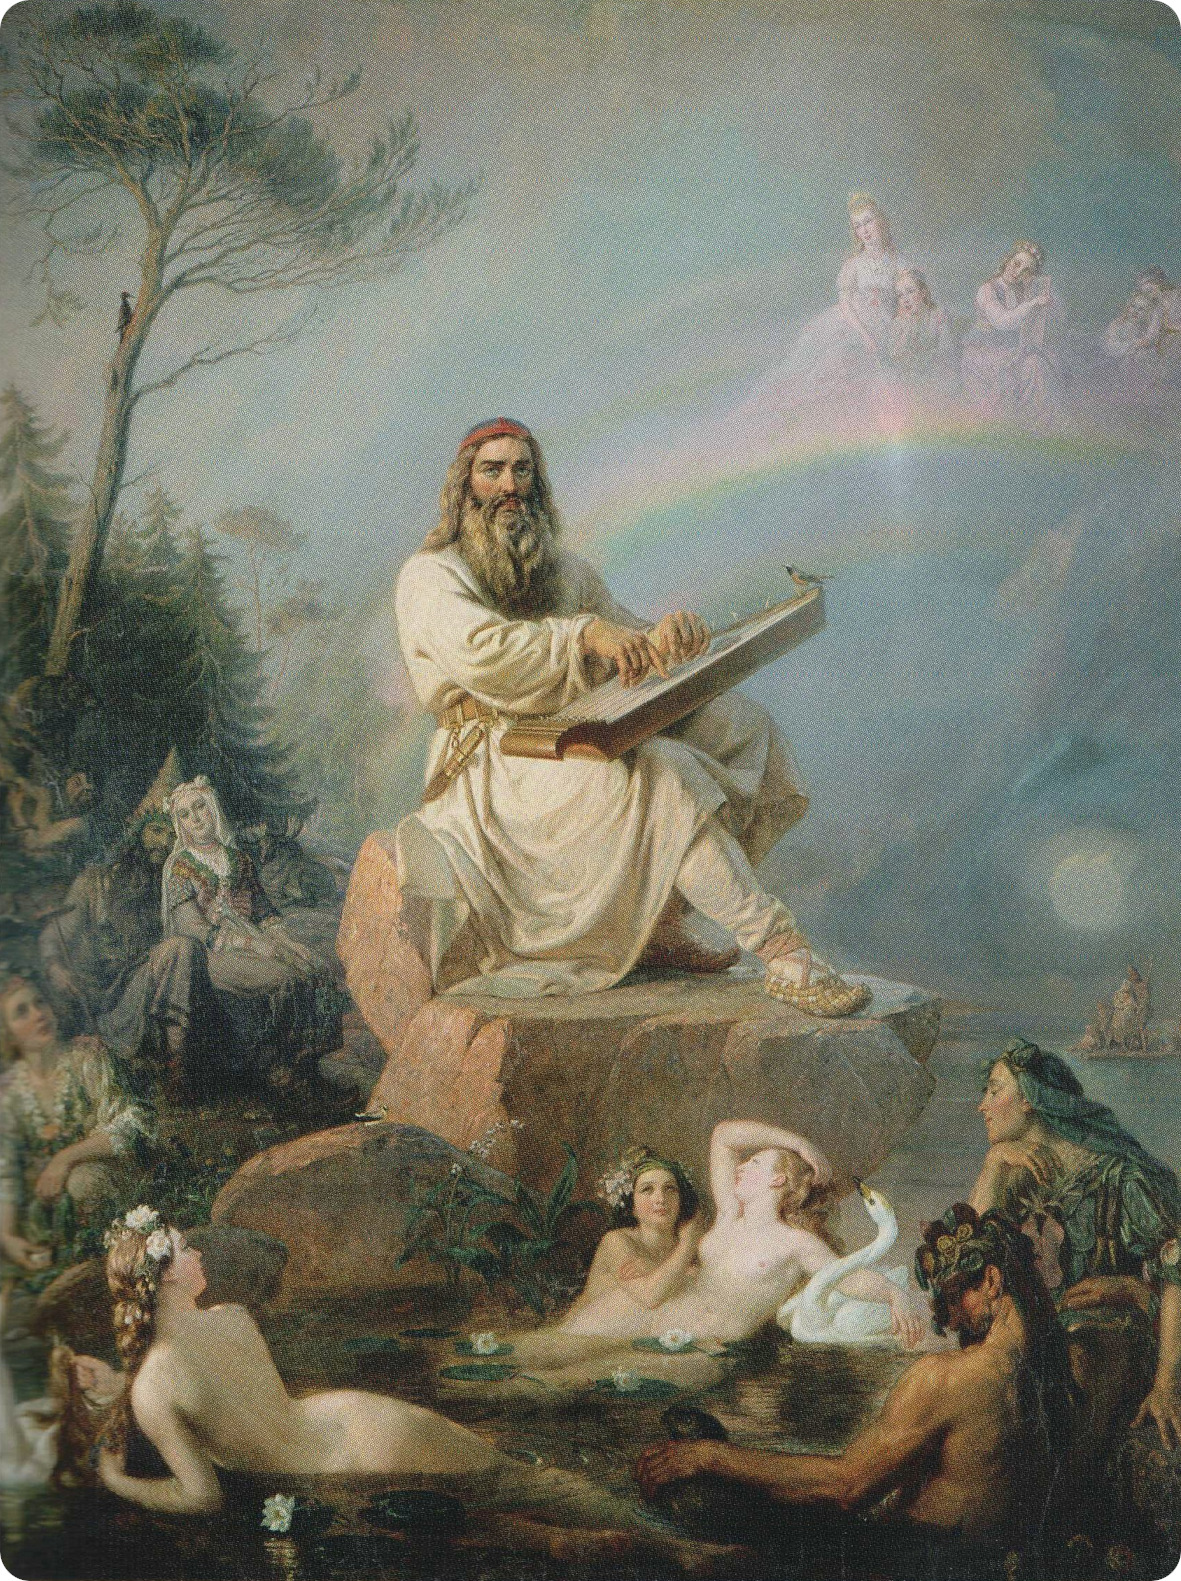
\includegraphics[width=0.82\textwidth]{Ekman_-_Vainamoisen_soitto.jpg}%
  \caption{R. W. Ekman: Väinämöisen soitto (1866)}%
\end{figure}
\vfill%


\clearpage
\subsection{Luonnon nostatus}
  \paragraph{}
  \begin{large}\begin{center}\begin{em}
    Luontoani nostattelen\\
    haastattelen haltijata\\
    Nouse luontoni lovesta\\
    Syntyni syvästä maasta\\
    Syntyni syvästä maasta\\
    \vspace{1em}
    Maasta hauna haltijani\\
    Nouse niin kuin nousit ennen\\
    Minun nostatellessani\\
    \vspace{1em}
    Isoni luonto, emoni luonto\\
    Luonto valta vanhempani\\
    Oman luontoni lisäksi\\
    Nosta Ukon voima taivahasta\\
    Maasta maan Emoisen voima\\
    \vspace{1em}
    Tuekseni turvakseni väekseni voimakseni\\
    Tulkaa tarvittaessa, käykää kutsuttaessa\\
    Terveyttä tekemään rauhaa rakentamaan\\
    \vspace{1em}
  \end{em}\end{center}\end{large}

  \paragraph{}
  %\begin{em}
    Eräs kielemme vanhimmista sanoista on ``noita'', joka on alunperin tarkoittanut tietäjää eli
    shamaania. Kristillisellä aikakaudella noita sai kielteisen kaiun. Sitä ennen tietäjät
    olivat arvokas osa yhteisöä, jonka jäseniä he tukivat sairauksissa ja elämän murroskohdissa.
    \par
    Sekä loveen lankeaminen että haltioituminen ovat tietäjien tapoja saavuttaa taianomainen
    mielentila, jossa he saavat apua esivanhemmiltaan tai suojelushengiltä.
  %\end{em}

  \paragraph{Lovi} on yliluonnollinen paikka tai olotila, aukko arkitodellisuuden ja alisen
    maailman välillä. Aliseen maailmaan kuuluu vainajala taikka Tuonela, jossa esi-isät asustavat.
    Lovi sijaitsee joko maan tai veden alla --- ilmeisesti myös naisten hameen alla, sillä
    kansanrunojen mukaan sieltäkin löytyy ovi tuonpuoleiseen. Osa muinaisista hautajaistavoistakin
    viittaa siihen, että vainaja pyrittiin palauttamaan takaisin kohtuun. Vainajalle tehtiin
    vertauskuvallisesti se, mitä sielulle toivottiin käyvän.
    \par
    Pohjolan emäntä Louhi, mahtava noita, tunnetaan myös muun muassa nimillä Lovetar ja Loviatar.
    Lovetar ilmenee syntysanoissa ja loitsun sanoissa. Louhi pystyy muuttamaan muotoaan,
    parantamaan, käskemään säätä, kuuta ja aurinkoa sekä synnyttämään mitä ihmeellisimpiä olentoja.
    Hänen kotinsa, myyttinen Pohjola, on pahojen asioiden, sairauden ja pakkasen lähde. Monet
    Pohjolan ongelmat, sairaudet ja harmit ovat itse Louhesta lähtöisin.
  \paragraph{Loveen lankeaminen:} Tietäjän matkaa vainajalaan kutsutaan loveen lankeamiseksi.
    Hurmoksessa tietäjä tekee sielunmatkan tuonpuolei\-seen ja käy kysymässä neuvoa esivanhemmilta.
    Suomalaiset tietäjät saattoivat vajota hurmokseen esimerkiksi raivoamalla, kun taas saamelainen
    \emph{noaidi} käytti apunaan rumpua. Loveen lankeamisessa käytettiin ehkä apuna myös laulamista
    [vrt. Väinämöinen laulaa Joukahaisen (Lapin tietäjän) suohon] ja soittamista (Väinämöisen
    jättihauenluinen kannel, jota kuunnelleessaan luomakunta lumoutui ja liikuttui).
    \par
    Väinämöinen lähtee Tuonelaan hakemaan puuttuvaa tietoa veneen rakentamiseen tai reen
    korjaamiseen. Joissain kertomuksissa hän hakee myös työvälineitä. Matkaa Tuonelaan
    kuvataan hyvin vaikeaksi ja vaivalloiseksi. Poiskaan sieltä ei ole helppo päästä, mutta
    Väinämöinen pakenee muuttumalla vesikäärmeeksi ja uimalla Tuonelan joen ylitse. Tämä
    viitannee muutokseen sieluneläimeksi, joiden joukossa käärmeet olivat suosittuja. Muutos
    sieluneläimeksi on yksi tietäjän keinoista.
  \paragraph{Lovesta nosto:} Loitsimalla saatetaan nostaa suvun esivanhempia eli omakuntaisia
    vainajalasta tälle puolen esimerkiksi suojelushaltijoiksi eli luonnoiksi.
  \paragraph{Luonto} on ihmisen tai muun tietoiseksi koetun olennon tai asian suojelushaltija.
    Alkuperäiseen merkitykseen viittaa ajatus jonkun luontumisesta. Luonnon katsotaann
    seuraavan ihmistä, suojelevan häntä ja tuovan hänelle onnea. Voimakasluontoiset eli ne,
    joilla on voimakas oma haltija, pärjäävät elämässä heikkoluontoisia paremmin. Luonto
    saattaa olla esimerkiksi vainajasta peräisin oleva esivanhempi eli \emph{syntyinen}.
  \paragraph{Luonnon kutsunta:} Jos ihmisellä on heikko luonto, hän saattaa joko kutsua itselleen
    vahvempaa luontoa tai voimistaa ja karaista luontoaan. Luontoa kutsutaan myös kateita,
    vihollisia ja sairauksia vastaan, ja antamaan lisää ruumiillisia, henkisiä tai yliluonnollisia
    kykyjä.
    \par
    Loitsuissa luonto nostetaan yleensä lovesta tai syvästä paikasta, vainajalasta. Joskus sitä
    kutsutaan nousemaan haon eli uppopuun alta. Joskus taas luontoa kutsutaan nousemaan ``haudan
    alta'', joka sekin viittaa siihen, että luonto on vainajalasta.
    \par
    Erään tiedon mukaan luontoaan saattaa karaista siten, että kohottaa juhlayönä järvestä hakoa
    ja kutsuu loitsulla luontoaan.
    \par
    Luontoa puhuteltaessa hänet ilmaistaan usein haltijaksi ja synnyksi. Tässä synty merkitsee
    joko myyttistä syntyä, esivanhemman sielua syntyistä tai molempia. Esimerkki loitsusta:

    \begin{center}\begin{em}
      Nouse luontoni lovesta,\\
      Syntyni syvästä maasta,\\
      Ha'on alta haltijani\\
      Vastuksia voittamah,\\
      Katehia kaatamah,\\
      Sotisia sortamahan\ldots\\
    \end{em}\end{center}

  \paragraph{Haltioituminen:} Ihmisen haltioituessa hänen luontonsa eli haltijansa hallitsee
    häntä. Tietäjät saattavat tavoitella haltioitumisen tilaa sairauksia parantaakseen tai
    muihin yliluonnollisiin tehtäviin.
    \par
    Nykyajan psykologiassa haltioituminen vertautuu lähinnä niin sanottuun flow-tilaan, jossa
    ihminen on syvästi keskittynyt tavoitteisiinsa. Joskus haltioituminen on käsitetty myös
    loveen lankeamisen vastineeksi tai taikojen harjoittamiseksi.
  \paragraph{Emuu} on olento, joka on synnyttänyt tai luonut jonkin kasvi- tai eläinlajin ---
    sen \emph{kantavanhempi} --- ja vastuussa tämän lajin toiminnasta sekä huolenpidosta.
    \par
    Metsästäjät pyytävät loitsuin kantavanhemmilta metsästysonnea. Pahaa voidaan yrittää karkottaa
    vanhempansa luo, tai uhata, että jos olento ei tottele, hänen käytöksestään kerrotaan hänen
    vanhemmalleen. Myös kantavanhempaa saatetaan käskeä panemaan lapsensa kuriin.
  \paragraph{Herättäjä} herättää ihmisen vaaran uhatessa. Jotkut väittävät omistavansa oman
    herättäjän, joka valvoo heidän untaan.
  \paragraph{Juhlia:} Nykyisistä juhlapyhistä laskiainen, helasunnuntai, juhannus, pyhäinpäivä ja 
    joulu olivat alun perin suomalaiseen alkuperäisuskontoon kuuluneita juhlia.


\subsection{Päivä, aurinko, kuu}

  \paragraph{Päivätär ja Kuutar:} Päivätär on elämää ja valoa hallitseva lämpöä ja hedelmällisyyttä
    antava hahmo. Kristillisellä kaudella hänet korvasi Neitsyt Maria. Hän on auringon ja päivän
    jumalatar, kaunis neito, jonka toveri tai kaksois\-olento on yhtä lailla kaunis kuun jumalatar
    Kuutar.
    \par
    Päivätär ja Kuutar omistavat auringon hopeaa ja kuun kultaa, joita näkyy kuun ja auringon
    hohteessa ja kultareunaisissa pilvissä auringonlaskun aikaan. Päivätär ja Kuutar näkyvät
    toisinaan Pohjolan tyttärien tavoin taivaalla kehräämässä kulta- ja hopealankaa kutoen
    siitä kultaisia ja hopeisia koruja ja vaatteita, joita neidot pyytävät kaunistuksekseen.

  \paragraph{Ilmarisen} mainitaan olleen mukana kosmisessa luomisessa, takomalla taivaankantta
    ja asettamalla taivaankappaleita.

  \begin{center}\begin{em}
    Tuli vanha Väinämöinen, ovelle asetteleikse.\\
    Sanan virkkoi, noin nimesi: ``Oi on seppo veikkoseni!\\
    Mitä paukutat pajassa, ajan kaiken kalkuttelet?''\\
    Se on seppo Ilmarinen sanan virkkoi, noin nimesi:\\
    ``Kuuta kullaista kuvoan, hope'ista aurinkoa\\
    tuonne taivahan laelle, päälle kuuen kirjokannen.''\\
  \end{em}\end{center}


\subsection{Maa}

  \paragraph{Akka} on Ukko ylijumalan nainen. Joskus hänet on tulkittu hedelmällisyyden
    jumalattareksi. Akka on luonnon naisellinen puoli, maaemonen, jonka Ukko hedelmöittää,
    ja sade saa viheriöimään. Näin saatiin aikaan maanviljelyn kannalta suotuisat ilmat.
    Akan mukaan on nimetty asteroidi \emph{8034 Akka}.
  \paragraph{Maan haltija} on nais- tai miespuolinen perhettä, taloa, satoa, karjaa ja pihapiiriä
    hoitava ja vartioiva hyvä haltija. Jos se on naispuolinen, menestyy karja hyvin, jos
    miespuolinen, menestyvät hevoset. Joskus haltijoita on pariskunta. Tällöin talo on erityisen
    onnekas.
    \par
    Haltijaa tulee kunnioittaa, niin hän hoitaa työnsä hyvin. Haltijalle on usein luvattu, että
    joka vuosi jonkun juhlan aikaan se saa osansa juhlaruuasta tai sadosta. Pyhä pihapuu on
    uhripaikka, jonka luona haltijaa kumarretaan ja sille viedään uhrilahjoja.
    \par
    Jos haltija on tavatessa hyvissä vaatteissa ja iloinen, ei hän ole onnettomuuden aiheuttaja,
    ja on vain varoittamassa. Jos haltija on pahoissa vaatteissa eikä näytä kasvojaan, on hän
    vihastunut, ja aikomassa aiheuttaa onnettomuuden. Erään perinteen mukaan tällöin on kiireesti
    mentävä paikalle, jossa haltija on näyttäytynyt, ja uhrattava alasti.
    \par
    Kun perustetaan uutta taloa, tehdään taikoja, jotta saataisiin haltija. Muuten voivat pahat
    haltijat tai maanväki asettua pihapiiriin. Erään kansanperinteen mukaan mukaan pitää polttaa
    tulta kolme päivää sillä paikalla, johon haluaa talon perustaa. Kolmantena päivänä haltija
    ilmestyy unessa. Silloin näkee, tuleeko mies- vai naishaltija vaiko pariskunta.
  \paragraph{Maahiset} eli \textbf{maanväki} ovat pieniä, ihmisenmuotoisia olentoja, jotka asuvat
    maan alla omassa maailmassaan. Usein maahisten maailma koetaan todellisen maailman
    peilikuvaksi, joka voi olla ylösalaisin.
    \par
    Maahiset voivat olla ilkikurisia. Metsässä saattaa joutua maahisten lumoihin ja eksyä
    nurinkuriseen maailmaan, jota \emph{metsänpeitoksikin} on kutsuttu. Maan väki voidaan käsittää
    myös taikavoimaksi, jota on maassa. Maanpäällisessä maailmassa maahiset ovat yleensä
    näkymättömiä. Maahisten kerrotaan myös lumoavan ihmisiä jäämään luokseen, jos ottaa vastaan
    heidän tarjoamiaan lahjoja, ruokaa tai juomaa.
  \paragraph{Sampsa Pellervoinen} kylvää maan kasvillisuuden, kaikenlaiset metsät, suot, ahot ja
    kivikotkin. Kylvö tapahtuu sammon murusten avulla. Hän on hedelmällisyyden haltija; hänet on
    rituaalisesti herätettävä joka kevät.
  \paragraph{Äkräs} on monipuolinen kasvillisuuden haltija. \emph{Loi herneet, pavut ja nauriit
    sekä antoi kaalit, pellavat ja hamput: Egres hernet Pawudh Naurit loi / Caalit Linat ia Hamput
    edestoi.}
  \paragraph{Jumi} on yliluonnollisten ilmiöiden, lähinnä panteistisen maailmanhengen nimitys.
    \emph{Marit} (volgansuomalainen kansa) viettävät vuosittain Jumolle omistettua juhlapäivää
    uhraten lihaa ja viljaa. Jumi aiheuttaa esimerkiksi eläimelle äkillisen taudin ampumalla
    näkymättömän nuolen. Arvoituksissa jumi on jokin, jolle on ominaista ehdoton paikallaanolo
    tai jota on mahdoton kiertää.

  % \subsubsection{Kivet}
    \paragraph{Kyllikki:} kivien emuu loitsuissa, joilla kiven aiheuttamia vammoja hoidetaan
  % \subsubsection{Käärme}
    \paragraph{Käres:} käärmeitten emuu
    \paragraph{Mammotar:} matojen emuu


\subsection{Meri ja vesi}

  \paragraph{Ahti:} veden jumala tai haltija
  \paragraph{Vellamo, Veen emonen, Veden emo} on hyvä ja arvostettu vedenhaltija, joka asuu veden
    alla Ahtolassa ja on Ahdin puoliso. Häntä palvotaan kalansaaliin toivossa ja purjehdussäähän
    vaikuttamaan.
    \par
    Vellamo on kaunis; hänellä on sininen lakki, kaislainen paita ja vaahtoinen vaippa.
  \paragraph{Iku-Turso} (myös \textbf{Meritursas} ja \textbf{Iku Turilas}) on vedenhaltija tai
    merihirviö, jonkinlainen alkuolento, joka on ollut olemassa maailman syntymästä lähtien.
    Runoissa se esiintyy usein Ison Tammen, maailmanpuun, kanssa.
  \paragraph{Väinämöinen}-nimen uskotaan juontuvan väinä-sanasta, joka tarkoittaa suvantoa tai
    hiljalleen virtaavaa vettä, salmea tai joensuuta. Väinämöisen lisämääreenä esiintyy myös
    \textbf{suvantolainen}.
    \par
    Väinämöinen on Ilmattaren, ilman immen ja meren poika. Hän viettää meressä kelluvan äitinsä
    kohdussa kolmekymmentä vuotta ja alkaa synnyttyään autella maailman luomisessa.
    \par
    Väinämöinen on taidokas veneenveistäjä. Hän tietää melkein kaiken tarpeellisen veneen tekoon,
    mutta ei kolmea ratkaisevan tärkeää sanaa, luotetta. Hän lähtee hakemaan niitä Tuonelasta,
    kuolleiden maasta. Väinämöinen käy myös ammoin kuolleen tietäjä Vipusen vatsassa tietoa
    hakemassa. Matka kuolleiden maahan on kuviteltu hyvin vaaralliseksi, vain mahtavien
    tietäjien on ajateltu pystyvän siihen ja tulemaan takaisin. Tässä on uistumia rituaaleista,
    joissa tietäjä vajoaa transsiin, ja hänen sielunsa liikkuu kuolleiden maailmassa suorittamassa
    tehtävää; suomalaisessa mytologiassa kerrotaan loveen lankeamisesta ja lovesta nostosta.
    \par
    Tuonen tytti toimii lautturina ja saattaa veneellään vainajat Tuonen mustan virran yli.
    Väinämöisen tytti kuitenkin huomaa olevan elossa. Väinämöinen valehtelee kuolleensa, mutta ei
    vakuuta. Tytti tietää millaisia ovat eri tavoin kuolleet: rautaan kuolleet ovat verisiä,
    hukkuneet vetisiä ja palaneet kärventyneitä. Väinämöinen kuitenkin lopulta pääsee Tuonelle.
    Tuonella hänet laitetaan nukkumaan vastenmieliseen sänkyyn tai paikkaan, joka on tehty
    käärmeistä tai täynnä käärmeitä. Hän onnistuu kuitenkin pakenemaan. Hän muuttuu vesieläimeksi,
    ja ui Tuonen joen poikki. Tuonen poika virittää rautaverkon veteen, mutta ei saa Väinämöistä
    tarttumaan. Väinämöinen palaa Tuonelta saatuaan haluamansa ja kertoo eläville Tuonelan
    oloista.
    \par
    Joissain runoissa kerrotaan, että Väinämöinen menee veneellään Rutjan koskeen, tuliseen
    pyörteeseen. Pyörre on usein tulkittu reitiksi Tuonelaan, vauhdikkaammaksi versioksi Tuonen
    joesta. Väinämöinen menee siis elävänä kuolleiden maahan. Väinämöisen veneenjäljeksi kutsutaan
    tyyntä kohtaa muuten aaltoilevalla vedenpinnalla.
    \par
    Vedenpinnan nimitysten lisäksi Väinämöiseen liittyviä nimityksiä löytyy luonnosta
    tähtitaivaalta, kuten Väinämöisen miekka tai viikate (Orion) ja Väinämöiset tai Väinämöisen
    virsut (Seulaset). Näitä tähdistöjä on käytetty suunnistamiseen vesillä. Väinämöisen
    arvellaankin alun perin liittyneen kiinteästi vesillä liikkumiseen.
    \par
    Kalevalassa Väinämöinen syntyy Ilmattaresta vanhana miehenä. Kansanrunoissa Ilmatar ei synnytä
    Väinämöistä, vaan Väinämöinen syntyy joko yksin tai Iro-neidosta.


\subsection{Ukkonen ja tuli}

    Samanistisessa kosmologiassa ihmisen maailma sijaitsee henkien asuttamien monikerroksisten ylä-
    ja alamaailmojen välissä. Joissain kansanrunoissa se kuvataan kodan pohjaksi, josta
    taivaankupoli rajaa henkien asuinsijat. Molemmissa ajatusrakennelmissa taivasta kannattaa
    maailmanpylväs ja taivaan napaa edustaa Pohjantähti.
    \par
    Käsitys sielusta kuuluu ikivanhaan pohjoiseen samanismiin. Sielun ja ruumiin pitkästä
    rinnakkaisuudesta kertoo muun muassa sukulaiskansojemme \emph{mansien} ja \emph{hantien} sana
    \emph{is}, joka on sukua suomen sanalle itse. Tähän liittyy löyly, joka sukukielissämme viittaa
    kylpemisen ohella sieluun.
  \paragraph{Ukko ylijumala} on muinainen sään ja sadon, ilman, oikeuden sekä ukkosen jumala, jota
    pyydetään avuksi esimerkiksi taisteluun tai taikuuteen ryhtyessä.
    \par
    Ukon lisänimen ``ylijumala'' voikin tulkita kahdella tapaa: joko, että hän todella on mahtavin
    (eli ylin), jumalista; tai pelkästään, että hän asuu ylhäällä taivaalla. Vahinkoa tekevän
    salamaniskun ajatellaan olevan Ukon rangaistus tai vihan ilmaus, ja elämää tuovan sateen
    hänen suopeutensa osoitus. Ukkoa muistuttava ukkosenjumala tunnettiin latvian kielessä nimellä
    \emph{Perkons} ja liettuan kielessä nimellä \emph{Perkūnas}, joista on peräisin suomen sana
    Perkele.
    \par
    Ukko iskee salamoita kirveellä, vasaralla, nuolella tai miekalla. Kokonaisen ukonilman hän saa
    aikaan puimalla riihtä, kyntäen, jyristellen vaunuillaan taivaissa, makaamalla naispuolisen
    jumaluuden kanssa, taikka kolisuttamalla konkeloa eli kelopuuta. Savukvartsia, josta
    iskettäessä syntyy kipinöitä ja palaneen hajua, nimitetään ukonkiveksi.
    \par
    Ukko kävelee pitkin askelin pilvien ja monikerroksisen taivaan yläpuolella, ja katselee
    ylhäältä maailmaa. Mahtavuudestaan huolimatta Ukko ei ole kaikkitietävä tai kaikkivaltias, vaan
    muilla henkiolennoilla ja ihmisillä on valtaa ja toimintatilaa. Ukon taivaallisessa
    valtakunnassa on heikompia henkiolentoja, joista perinteet tuntevat muun muassa päivättäret,
    kuuttaret, ilman immet, kapeet, kuumet, tuulettaret ja muita.
    \par
    Ukon kerrotaan myös pitävän pilvissä käräjiä, joten voisi olettaa, että taivaalla asuu tai
    ainakin vierailee muitakin merkittäviä henkiolentoja, joiden kanssa Ukko päättää asioista.
    Ukkoa rukoillaan pitämään käräjiä eri ongelmien voittamiseksi.

  \paragraph{Kokko} tai \textbf{vaakalintu} on jättiläismäinen kotka, sukua yleismaailmalliselle
    ukkos\-lintuhengelle, joka tunnetaan Euroopasta aina Amerikan alkuperäiskansoille asti. Se
    voi olla muistumaa ihmishahmoista jumaluutta edeltäneestä käsityksestä, jonka mukaan taivasta
    ja ukkosta hallitsee ukkoslintu. Ukkoslintuihin uskovat paitsi jotkin suomalais-ugrilaiset,
    myös monet muut kansat.
    \par
    Kokon mittasuhteet kuvataan joskus valtaviksi: toinen siipi haroo taivasta, kun toinen
    koskettaa meren luotoja.
    \par
    Kokko ja Ilmarinen osallistuvat yhä joissain tulen syntysanoissa ensimmäisen tulen iskentään,
    joka toisissa perinteissä on Ukon tehtävä. Kokko on toisinaan tarusankarien ystävä, toisinaan
    vihollinen. Joskus sen tehtävä on vartioida. Kokko kuvataan joskus rautaiseksi, joskus
    tuliseksi. Kokko pystyy kantamaan ihmistä. Se iskee tulta auttaakseen Väinämöistä polttamaan
    kasken. Myös kokon sulkia käytetään tulen iskemiseen. Joissain tulen syntykertomuksissa tuli
    on isketty kokon sulilla.
    \par
    Kokkoja voi olla useita. Eräs näistä pelastaa Väinämöisen merihädästä palkkioksi siitä, että
    kaskea kaataessaan Väinämöinen jätti koivun linnuille istumapuuksi. Ilmarinen ja Louhi tekevät
    omat kokkonsa. Ilmarinen tekee metallisen kokon, joka pyydystää suomuhauen. Louhi taas muuttuu
    itse kokoksi rakentamalla siivet ja pyrstön laivan osista ja ottamalla viikatteet
    kynsiksi.
    \par
    Sanassa vaakalintu esiintyvä ``vaaka'' tulee mahdollisesti sanasta ``vaa’as'', joka tarkoittaa
    myyttistä tulta, aaltoa ja kipua. Toinen mahdollisuus on ``vuokko'', saamelaisten kertomusten
    tietäjän apulintu.
  \paragraph{Panu} on tulen henki, auringon poika. Panuun voi vedota loitsuissa, kun ollaan
    tekemisissä tulen kanssa.


\subsection{Ilma ja tuuli}

  \paragraph{Ilmattaret} eli \textbf{Ilman immet} ovat taivaalla asuvia jumalaisia neitoja, jotka
    muistuttavat Pohjan neitoja, sillä nekin istuvat ajoittain taivaankannella.
    \par
    Ilmatar liittyy Väinämöisen ja maailman syntymään. Ilmatar tylsistyy oloonsa impenä taivaalla
    ja laskeutuu meren selälle. Tuuli hedelmöittää hänet. Sotka etsii pesäpaikkaa ja huomaa
    Ilmattaren polven, jolle se tekee pesän ja munii siihen munansa. Polvea alkaa kuumottaa ja
    Ilmatar heilauttaa sitä, jolloin munat putoavat ja särkyvät. Särkyneistä munankuorista syntyy
    maailma.
  \paragraph{Seppo Ilmarinen} on Väinölässä asuva seppäsankari, jolla on jumalallisia piirteitä.
    Häntä pidetään myös tuulen, sään ja ilman jumalana, joka on mukana maailman syntymässä.
    \par
    Iro-neito synnytti Ilmarisen yöllä ja jo päivällä Ilmarinen teki pajan. Palkeet liittyvät
    Ilmarisen asemaan tuulen jumalana, mutta toisaalta myös tämän rooliin kosmisena seppänä.
    Ilmarisen taontatyö ei onnistu ennen kuin hän tarttuu palkeisiin orjien sijasta itse.
    Ilmarinen takoi maailman alussa taivaankantta niin taidokkaasti, etteivät näy pihtien pitämät,
    eivätkä tunnu vasaran iskut. Ilmarisen kädenjälkeä ovat myös revontulet, aamu- ja iltaruskon
    värit. Myös raudan keksiminen ja alkutulen iskeminen ovat Ilmarisen saavutuksia. Ilmarinen
    takoo monia esineitä, kuten Sammon, Kultaisen naisen, ja yrittää takoa uuden Auringon ja Kuun.
    \par
    Suomalaisilla lienee ollut Ukkoa aikaisempi, omaperäinen taivaan jumala. Tämän syrjäydyttyä
    Ukon tieltä siitä kehittyi kalevalaisen perinteen seppäsankari Ilmarinen. Ilmarisen asemasta
    taivaan jumaluutena on säilynyt muistumia myytteihin, kuten uskomukset, että hän takoi
    taivaankannen ja Sammon, joka alkujaan käsitettiin taivaan tukipylvääksi.
  \paragraph{Sielulintu} on sielun koti ja vertauskuva. Lintu ehkä tuo sielun syntymässä ja vie sen
    kuoleman hetkellä. Joidenkin perinteiden mukaan nukkuessa on hyvä olla lähellä puusta
    veistetty sielulintu, joka pitää huolta sielusta unen aikana, jottei se lähtisi omille
    teilleen. Ihmisen kuoltua hänen puinen sielulintunsa laitetaan ortodoksisen hautaristin
    yläpuolelle. Lintujen ruokkiminen jouluna on vanha tapa; kuolleet eli sielulinnut ovat elävien
    kanssa mukana keskitalven juhlassa.
    \par
    Samanistisessa ihmiskuvassa sielu on usein monikerroksinen. Sen osista yksi saattaa unessa tai
    transsissa liikkua kehon ulkopuolella esimerkiksi linnun hahmossa. Lintujen merkitys
    suomalais-ugrilaisille näkyy siinäkin, että taivaan halkaisevan galaktisen vyön nimi on
    Linnunrata.
  \paragraph{Tuuletar} tarkoittaa naispuolista tuulta hallitsevaa luonnonhenkeä tai tuulen
    personoitumaa. Tuulettaria on erilaisia. Tuuletar saattaa olla yksittäinen tuulenpuuska,
    vihuri tai tuulispää, tai tietynlainen jatkuva tuuli. Tuuletar voi myös olla tuulen jumala,
    jolta pyytämällä saa suotuisaa ilmaa. Tietty tuuletar voi myös vastata tietystä ilmansuunnasta
    tulevaa tuulta.
  \paragraph{Tapiotar:} lintujen emuu


\subsection{Metsä}

  \paragraph{Tapio} on metsän haltija ja hän hallitsee metsäistä valtakuntaansa Tapiolaa. Tapion
    väki kaunistaa ja siivoaa metsää, huolehtii kasveista ja eläimistä. Tapion tyttäriä ovat
    ihastuttavat Tellervo, Tyytikki, Tuulikki ja Annikki. Tapiota ja hänen perhettään kuvaillaan
    ihmishahmoisiksi ja joko alastomiksi tai kauniisti pukeutuneiksi. Joidenkin runojen mukaan
    Tapion parta on puuta ja silmät kuin kaksi pohjatonta järveä.
  \paragraph{Mielikki} on Tapion vaimo. Metsästäjien on puheltava ja laulettava viettelevästi ja
    imartelevasti Mielikille saadakseen tältä lahjana saalista. Mielikki hoitaa metsän ``taloustyöt''
    eli siistimisen, koristelun ja kaunistamisen. Metsän kauneutta, kuten myös Mielikin omaa
    kauneutta, kannattaa metsässä liikkuessa kehua. Mielikin uskotaan lepyttävän miestään Tapiota,
    jos tämä tulee huonolle tuulelle ja usuttaa voimat metsämiehiä vastaan.
    \par
    Harvoin ihmisille näyttäytyessään Mielikki usein huvikseen pukeutuu Tapion harmaaseen
    naavaturkkiin ja -hattuun. Katsojan silmissä kuu\-sikossa kulkee höperö vanhus, joka laskee
    mättäiden marjoja.
    \par
    Mielikki on taitava parantaja. Hän hoitaa ansoihin jääneet käpälät ja tassut, pesästä pudonneet
    linnunpoikaset ja metsokukkojen taisteluhaavat. Metsän parantavat kasvit hän kerää
    huolellisesti talteen, ja niinpä hänellä on sopivia rohtoja myös ihmisten vaivoihin, jos joku
    vain keksii käydä pyytämässä. Mielikin käyttämiä kasveja ovat muun muassa kanerva ja kataja.
    \par
    Pienriistan pyytäjän, sienestäjän ja marjastajan kannattaa lausua metsään mennessään:
    \emph{``Siniviitta, viidan eukko, / mieluinen metsän e\-mäntä! / Anna tie, avaa portti / minun
    metsällä käydessäni.''} Mielikin nimi juontuu onnea ja kohtaloa merkinneestä mielu-sanasta.
  \paragraph{Tyytikki:} oravien emuu; Tapion ja hänen puolisonsa Mielikin tytär
  \paragraph{Metsän haltijat ja olennot:} Metsässä on myös arvaamattomampia tai vihamielisiä
    olentoja, kuten maahisia, metsähiisiä, menninkäisiä ja keijuja. Nämä saattavat sairastuttaa,
    eksyttää tai lumota, jos tulee näiden valtapiirille. Menninkäiset saattavat eksyttää metsässä
    kulkevan nurinkuriseen maailmaan. Metsässä saattaa olla myös noidankehä, alue, johon joutunut
    lumoutuu. Tätä saattaa merkitä esimerkiksi sienien itiöemien muodostama kehä.
    \par
    Metsän väkeä asuu muun muassa muurahaiskeoissa, puunkoloissa, kivenkoloissa, juurakoissa ja
    kannoissa. Väen taikavoimaa saattaa löytää myrskyn katkaisemien puiden murtumakohdista tai
    yhteenkasvaneista puista. Avoimella paikalla kasvava yksinäinen puu on tärkeä metsänväen
    kokoontumispaikka.
  \paragraph{Metsänneito} (myös \textbf{metsänneitsyt}, \textbf{metsänpiika}, \textbf{sinipiika})
    ilmaantuu joskus metsässä liikkuville tai yöpyville miehille: se saattaa tulla tanssimaan
    nuotiolle tai kävellä vastaan. Metsänneitsyt oli edestäpäin ihastuttavan kaunis, harsopukuinen
    ja pitkähiuksinen, mutta olennon selkäpuoli on ontto tai takaa se on vain puupökkelö. Tämän
    huomaaa kauhukseen mies, jos yrittää nähdä neidon selkäpuolen. Tällöin metsänneitsyt pelästyy
    ja lähtee.
  \paragraph{Menninkäinen} on yksinäisillä paikoilla asustava pieni ja pimeästä pitävä olento, joka
    on yleensä ihmisille suopea. Sana on ilmeisesti alun perin tarkoittanut vainajaa ja manalaista.
    Menninkäiset eivät välttämättä kestä päivänvaloa. Ne ovat vieraita ja outoja olentoja, joiden
    motiivit ovat ihmisille tuntemattomat, päin vastoin kuin tiettyihin elementteihin liittyvien
    väkien.
    \par
    Menninkäiset ovat voineet tulla mellastamaan kirkkoon öisin, jolloin niitä on pidetty pikku
    paholaisina. Ne saattavat pälyillä ihmisiä ikkunan tai puunrungon takaa, tai istuskella ryhmänä
    kivellä ihmistä tuijottaen. Menninkäiset järjestävät mielellään pitoja, joissa syödään, juodaan
    ja tanssitaan. Menninkäiset pitävät kiiltävistä esineistä.
  \paragraph{Ajattara:} paha naispuolinen olento, joka ajaa metsämiehiä ja metsästäjiä harhaan.
  \paragraph{Hongatar:} ärtyisä ja rujo karhujen emuu, honkien suojelija
  \paragraph{Juonetar:} peurojen emuu
  \paragraph{Käreitär:} kettujen emuu
  \paragraph{Laus:} porojen ja hirvien emuu
  \paragraph{Äimätär:} susien emuu


\subsection{Puut}

  \paragraph{Kati:} puiden emuu --- metsän kaunis ja nuori jumalatar, joka synnyttää puita
  \paragraph{Elämänpuu:} Nainen nähdään elämän ja kuoleman sekä niitä vastaavien ilmansuuntien
    etelän ja pohjoisen hallitsijana. Tämän äitihahmon mielikuvastoon liittyvät myös aurinko ja
    elämänpuu, joka usein mielletään koivuksi.
    \par
    Kalevalassa Iso Tammi kohoaa peittämään koko taivaankannen ja se lopulta kaadetaan. Aihelmaa
    on selitetty Linnunradan syntynä, sillä Linnunrata muistuttaa muodoltaan kaadettua puuta.
  \paragraph{Koivu:} \emph{[vesi]} suojelu, puhdistaminen. Koivunoksia on käytetty kautta aikain
    karkottamaan pahoja henkiä ihmisestä vihtomalla.
  \paragraph{Poppeli:} \emph{[vesi]} vauraus, lentäminen
  \paragraph{Haapa:} \emph{[ilma]} suojelee varkauksilta, parantaa ilmaisukykyä
  \paragraph{Mänty:} \emph{[ilma]} parantaminen, hedelmällisyys, vauraus
  \paragraph{Pihlaja:} \emph{[tuli]} psyykkiset voimat, parantaminen, voima, menestyminen, suojelu
  \paragraph{Tammi:} \emph{[tuli]} suojelu, terveys, vauraus, paraneminen, potenssi,
    hedelmällisyys, onni
  \paragraph{Saarni:} \emph{[tuli]} suojelu, terveys, mereen liittyvät rituaalit, vauraus
  \paragraph{Kataja:} \emph{[tuli]} suojelu, varkauksien esto, rakkaus, terveys


\subsection{Tieto}

  \paragraph{Antero Vipunen} on maan alla makaava vainaja tai jättiläinen; tietäjä, jolla on
    hallussaan arvokkaita ikiaikaisia loitsuja tai tietoja.
    \par
    Väinämöisen loitsusta puuttuu kolme sanaa eli luotetta. Ne saadakseen hän menee herättämään
    nukkuvan Vipusen joko hakkaamalla puut tämän haudalta tai menemällä suusta vatsaan. Vipunen
    voi myös nielaista Väinämöisen. Vatsassa Väinämöinen takoo niin kovasti, että Vipunen
    luovuttaa ja antaa sanat vatsakivusta päästäkseen.
    \par
    Viron kielessä \emph{vibu} on jousipyssy, joten Virossa Vipunen on käsitetty taitavaksi
    jousimieheksi. Useissa kertomuksen versioissa Vipusen mainitaan olevan ansastaja, kuten
    nimestä Vipunen voi päätellä. Vipusen arvellaan lainatun saamelaisista tarinoista, joissa
    käytiin noita Antereeuksen haudalla hakemassa tietoja.
  \paragraph{Väinämöinen} on taidokas loitsujen laulaja, kanteleen soittaja ja suuri tietäjä:
    \emph{``Vaka vanha Väinämöinen / Tietäjä iän ikuinen''}. Hän veistää veneen laulamalla.
    \par
    Sotajoukon laiva pysähtyy jättiläismäisen suomuhauen selkään. Hauki tapetaan, ja sen
    leukaluusta Väinämöinen tekee kanteleen. Kanteleen kielet hän saa jonkin Hiiden olennon
    hiuksista. Väinämöinen soittaa kanneltaan niin taidokkaasti, että ihmiset, eläimet ja
    jumalolennotkin tulevat kuuntelemaan, eikä ole karskeintakaan urosta, joka ei liikuttuisi
    kyyneliin.
    \par
    Eräässä yleisessä kansanrunossa Väinämöinen syntyy yöllä, tekee päivällä pajan, takoo
    rautaisen hevosen, ja ratsastaa sillä veden päällä. Joukahainen on nuori ja laiha Lapin
    tietäjä, joka kadehtii Väinämöisen laulutaitoja ja matkustaa kolme päivää haastamaan tämän
    miekan mittelöön. Väinämöinen ei suostu miekkailemaan. He loihtivat kilpaa, jonka päätteeksi
    Väinämöinen laulaa Joukahaisen suohon. Pelastautuakseen Joukahainen lupaaa Väinämöiselle
    siskonsa Ainon puolisoksi. Aino hukuttautuu, sillä hän ei halua vaimoksi vanhalle
    Väinämöiselle. Väinämöinen ratsastaa veden päällä, ja Joukahainen ampuu hänet kostoksi
    alkumereen.
    \par
    Aiemmissa runoissa Väinämöinen ja Joukahainen ovat saman äidin, Iro-neidon lapsia. He lähtevät
    yhtä matkaa kulkemaan, mutta ajautuvat erilleen ja käyvät toistensa kimppuun. Väinämöinen
    voittaa taikansa avulla. Maailmankaikkeus syntyy, kun sotka munii munansa Väinämämöisen
    polvelle Joukahaisen suistettua hänet veteen. Väinämöinen kelluu vedessä, kun vesilintu, sotka,
    pesii hänen polvelleen. Haudonta polttaa polvea, jolloin Väinämöinen vavahduttaa sitä.
    Linnun munat joutuvat mereen, hajoavat ja synnyttävät maailman. Kalevalassa sotka munii
    Väinämöistä odottavan ilmattaren polvelle, eikä Väinämöisen polvelle, kuten kansanrunoissa.
  \paragraph{Väinämöisen paluu?} Neitsyt Marjatta tulee raskaaksi puolukasta ja saa poikalapsen
    tai lapsi löytyy metsästä, jolloin etsitään turhaan myös äitiä. Väinämöinen määrää lapsen
    äpäränä suolle vietäväksi ja puulla päähän lyötäväksi. Sylilapsi alkaa puhua, syyttää
    Väinämöistä pahemmista synneistä ja huomauttaa, ettei Väinämöistäkään ole niiden takia viety
    suolle. Lapsi kastetaan Kaukomieleksi Karjalan kuninkaaksi.
    \par
    Väinämöinen suuttuu, häpeää ja poistuu vaskisella ja kuparisella veneellään, ja sanoo
    palaavansa, kun häntä tarvitaan, etsitään ja kaivataan. Samaan tapaan vesitse ja kristinuskon
    ahdistamina ovat poistuneet myös Kalevanpojat, mutta he soutivat kivellä.


\subsection{Hiisi}

  Hiisi on pyhä kulttipaikka, pyhä lehto ja mahdollisesti kalmisto. Hiideksi on myös myöhemmin
  alettu kutsua kulttipaikalla palvottua henkiolentoa, kalmiston vainajien yhteensulautuneiden
  henkien muodostamaa kollektiivia.
  \par
  Kristinuskon saapumisen jälkeen hiisi on ollut paha henkiolento ja paha paikka. Hiisistä
  muodostui kansantarinoihin pieniä pahoja tai vähintään tuhmia olentoja, joiden kotipaikka oli
  myös nimeltään Hiisi, tai joskus Hiitola. Metsähiisi ja vesihiisi olivat metsässä ja vedessä
  asuvia hiisiä, mutta myös sairauksien nimiä. Myös pyhästä hauta-alueesta tai helvetin kaltaisesta
  paikasta saatettiin puhua hiitenä. Myöhemmin hiisi-sana alkoi viitata pakanalliseen
  henkiolentoon, pienikokoiseen ilkeään haltiaan tai peikkoon.
  \par
  Kalevalassa Väinämöinen joutuu taistelemaan Lempoa, Pahaa ja Hiittä vastaan. Hiisien kotipaikka
  Hiitola sijaitsee vaikeakulkuisessa maastossa, syrjässä ihmisasutuksesta. Hiittä pahana paikkana
  on peräpohjolassa kutsuttu sanalla helsinki. Joskus hiisi rinnastetaan myös jättiläisiin tai
  vuorenpeikkoihin.
  \par
  Hiitolaan on rakennettu Hiiden linna, jossa Hiisi asuu Hiiden emännän kanssa. Hiiden emännältä
  Väinämöinen saa kanteleeseensa kielet. Hiiden linnassa asuu myös hiitolaisia --- joiden hiukset
  olivat käärmeitä --- sekä Hiiden raivoava rakki ja Hiiden kissa, Kipinätär nimeltään. Hiidellä
  on myös Hiiden ruuna, hiisien nopea hevonen ja yksi ainoa tytär, Hippe. Hipen tehtävänä on
  laittaa varkaat palauttamaan varastettu omaisuus oikeille omistajilleen. 

  \paragraph{Hiiden hirvi} on vaikeasti pyydystettävä, voimakas ja nopea hirveä muistuttava olento.
    Se saattaa olla samaa kantaa kuin samojedien ja obinugrilaisten taivaallinen peura,
    kuusijalkainen olento, jonka ensimmäinen samaani pyydysti. 


\subsection{Pohjola}

  Pohjolan emännän valtakunta kuvataan pahaksi ja kylmäksi maaksi kaukana pohjoisessa. Pohjola
  on sekä sankarien vihollinen, että pahojen asioiden, kuten pakkasen ja sairauksien, alkulähde.
  Pohjolan hyviä oloja kuitenkin kadehditaan, eivätkä kielteiset käsitykset estä kalevalaisia
  sankareita matkaamasta kohti Louhen valtakuntaa ja kosiskelemasta hänen yliluonnollisen kauniita
  tyttäriään.

  \paragraph{Pohjolan emäntä} eli \textbf{Pohjan akka} johtaa myyttistä Pohjolaa. Kalevalassa
  Pohjolan emännän nimi on \textbf{Louhi}, mutta tunnetaan muitakin nimiä: \textbf{Lovetar},
  \textbf{Loviatar}, \textbf{Louheatar} ja \textbf{Lovehetar}. Häneen viitataan säeparilla:
  \emph{``Louhi Pohjolan emäntä / Pohjan akka harvahammas''}.
  \par
  Pohjolan emännällä on suunnattomat taikavoimat: hän pystyy muuttamaan muotoaan, käskemään säätä,
  säätämään auringon ja kuun kulkua, parantamaan ja on kykeneväinen synnyttämään mitä
  ihmeellisimpiä olioita. Hän varustaa sotaveneen soutajineen ja sotaväkineen, ja veneen
  tuhouduttua ottaa veneen laidat siivikseen, ja muuntautuu jättimäiseksi Kokko-linnuksi, jonka
  selkään soturit nousevat.
  \par
  Pohjolan emäntä on synnyttänyt monia ongelmista, jotka tulevat Pohjolasta ihmisten harmiksi.
  Hänet on usein portoksi mainittu siksi, etteivät nämä ``lapset'' ole avioliitosta peräisin. Hänet
  hedelmöittää tuuli, kun hän paljastaa alapäänsä pohjoiseen päin, tai sen tekee Iku-Turso meren
  kuohuilla kovilla.
  \par
  Louhi mainitaan usein myös ihmeellisten Pohjolan neitojen äidiksi. Pohjolan isäntä jää yleensä
  sivuosaan. Yleensä miestä ei mainita ollenkaan, ja paheksuen korostetaan, että emäntä luo
  synnyttämänsä asiat ja olennot luonnottomasti ja aviottomasti.


\subsection{Sampo}

  Sampo on ihmeellinen, rikkauksia tekevä mylly: kirjokansi, ihmekone, joka jauhaa rahaa, viljaa ja
  suolaa. Sampo jauhaa, sillä maailmanpylvään on ajateltu kiertyvän taivaankannen mukana. Sillä
  arvellaan myös olevan jalat, joiden avulla se seisoo, sekä reiät tai nokat. Sammon juuret ovat
  syvällä maaemässä, ja Sammon yleinen toisintonimi on kirjokansi, joka viittaa taivaankanteen.
  Sammas on patsas, joka kannattaa taivaan kantta. Kultanappi tai kultainen naula on pohjantähti
  (tai Vega, joka oli 12 000 vuotta sitten Pohjantähden kohdalla), joka kiinnittää taivaankannen
  ja maan. Taivaankansi pyörii naulan ympäri: ``sammas jauhaa''. Myös indoeurooppalaisilla kansoilla
  on maailmanpylväsmyytti. Esimerkiksi Intiassa pylvästä kannattelee kilpikonna.
  \par
  Sampo-tarut ovat, paitsi ihmeellisiä kertomuksia kahden kansan taistelusta ja ihme-esineen
  vaiheista, alkujaan kosmisia kuvauksia. Ne selittävät maanviljelyksen syntyä ja muidenkin
  asioiden myyttistä alkuperää. Sampo on esiintynyt myös nimillä sampa, sammas, sampi, sampu,
  samppu, samppo ja sammut. Sanana sampo on sukua sammakselle eli pylväälle. Laajalti esiintyviä
  sammon piirteitä ovat hyvyys, kirjokanteen viittaus ja yhteys merelliseen Pohjolaan. Sampo
  liitetään seppien tuomaan uudenlaiseen hyvinvointiin, joka uhkaa sysäyttää Väinämöisen ja
  tietäjäkulttuurin.
  \par
  Väinämöinen lähtee Pohjolaan kosimaan Pohjolan tytärtä. Pohjolan emäntä a\-settaa kosijalle
  ehdoksi, että Väinämöisen on taottava sampo. Väinämöinen ei tähän pysty, ja hän lähtee pettyneenä
  kotiin. Hän kuitenkin lähettää sepän, Ilmarisen, takomaan Pohjolaan sammon. Seppo Ilmarinen takoo
  Sammon Pohjolan emännälle vastineeksi Pohjolan tyttärestä. Pohjolan emäntä Louhi ottaa Sammon
  vastaan, mutta kieltäytyy luovuttamasta tyttöä Ilmarisen vaimoksi. Louhi vie Sammon kivisen mäen
  sisään, juurruttaa sen maaperään, ja sulkee lukkojen taakse. Sen jälkeen sampo jauhaa rikkautta
  Pohjolan väelle. Tästä suuttuneina kalevalaiset hyökkäävät Pohjolaan ja anastavat Sammon.
  Syntyneessä taistelussa sampo tuhoutuu. Pohjan Akka saa Sammon kannen. Sammon sirpaleita
  ajelehtii kalevalaisten rantaan, ja ne saavat maanviljelyn aikaan.

  \begin{figure}[!hb]%
    \centering%
    % 0.618034^2 ~ 0.381966 (Golden Ratio)
    \includegraphics[width=.381966\textwidth]{pohjannaula_transparent_bg_525x452px.png}%
    \caption{Pohjantähti naulana liittää yhteen kuvun muotoisen taivaankannen ja sampaan eli maailmanpylvään. E. N. Setälän (1932) mukaan.}%
  \end{figure}


\subsection{Kirjallisuutta}

  \begin{itemize}
    \item Siikala, Anna-Leena: \emph{Itämerensuomalaisten mytologia}. Hämeenlinna: SKS, 2012.
    \item Siikala, Anna-Leena: \emph{Suomalainen šamanismi}. Hämeenlinna: SKS, 1992.
    \item Haavio, Martti: \emph{Suomalainen mytologia}. Porvoo Helsinki: WSOY, 1967.
    \item Ganander, Kristfried: \emph{Mythologia Fennica}. Turku: Frenckell, 1789.
    \item Emil Nestor Setälä: \emph{Sammon arvoitus: Isien runous ja usko}. Helsinki: Otava, 1932.
    \item \emph{SKVR-tietokanta}. \url{https://skvr.fi/}
  \end{itemize}

  \paragraph{}
    {\small
      Muinaissuomalaista mytologiaa ---luvun ensimmäisen version kokosi \emph{antagomir}.
    }

  \paragraph{}
    {\small
      \emph{``Nimi-instituution puuttumisesta siis johtunee, ettei vanhimmilla ihmishahmoisilla
      jumaluuksillakaan ollut erityistä nimeä, vaan naisjumaluudet olivat akkoja, jotka erotettiin
      toisistaan asuinsijojensa, tehtäviensä tai aseittensa mukaan. Toisin sanoen: akka-jumaluudet
      tuntuisivat siis olevan ajalta, jolloin uralilaiset/suomalais-ugrilaiset eivät vielä olleet
      omaksuneet kantaeuroopasta lainasanaa nimi ja siihen liittyvää nimenantoa ja proprin-käyttöä.
      Mutta akkojen aika saattoi senkin jälkeen jatkua yksinomaisena pitkään, kunnes
      kantasuomalaisten taivaalle ilmaantui kantaeurooppalainen ukkosenjumala Ilmamoinen; hän
      tarvitsi ja sai nimen. Akkojen aika kesti siten koko neljännen vuosituhannen ja suuren osan
      kolmattakin. Eivätkä akkajumalat hävinneet senkään jälkeen: Pohjan akka ja akka manteren
      alainen elivät kalevalaisessa perinteessä entiseen tapaan nimettöminä lähes nykyaikaan
      asti.''} --- Unto Salo, ``Tuoni, Pohjola, Taivas --- Arkeologian ja kalevalaisten runojen
      tuonelat (Kalevalaiset myytit ja uskomukset III)'', s. 115
    }


      \clearpage\scleardpage
      \section{Runoja, loitsuja}
        \begin{songs}{titleidx,authidx,tagidx}
          \chordsoff % songs: do not show (empty line for non-existing) chords
          % songs: Increase line spacing for better readability
          \baselineadj=+1pt plus 0pt minus 0pt%
          \renewcommand{\lyricfont}{\small} % songs: use smaller font
          \songcolumns{2} % songs: two columns per page
          \songpos{1} % songs: avoid ONLY page-turns within songs
          % songs: make penalty for breaking column/page at any line of lyrics to be the same:
          % (The default for \interlinepenalty is 1000, and for all the others 200.)
          \interlinepenalty=200 %
          % Finnish spells and poems
% ========================
%
% The following sets the song number for the first song in this file.
% The number will automatically be incremented by one for each song.
% Please do not change this! Changing would make different versions of
% the songbook to have different numbers for the same songs, and it
% would totally mess up the selection booklets causing them to have
% wrong songs in them. (For the same reason, add new songs only to the
% end of each songs_ file.)
\setcounter{songnum}{700}


\beginsong{\texorpdfstring{Maailmansynty\-runo}{Maailmansyntyruno}}[by={Kalevala: 1. runo}]
  \beginverse
    Mieleni minun tekevi,
    aivoni ajattelevi
    lähteäni laulamahan,
    saa'ani sanelemahan,
    sukuvirttä suoltamahan,
    lajivirttä laulamahan.
    Sanat suussani sulavat,
    puhe'et putoelevat,
    kielelleni kerkiävät,
    hampahilleni hajoovat.
    Veli kulta, veikkoseni,
    kaunis kasvinkumppalini!
    Lähe nyt kanssa laulamahan,
    saa kera sanelemahan
    yhtehen yhyttyämme,
    kahta'alta käytyämme!
    Harvoin yhtehen yhymme,
    saamme toinen toisihimme
    näillä raukoilla rajoilla,
    poloisilla Pohjan mailla.
  \endverse
  \beginverse
    Lyökämme käsi kätehen,
    sormet sormien lomahan,
    lauloaksemme hyviä,
    parahia pannaksemme,
    kuulla noien kultaisien,
    tietä mielitehtoisien,
    nuorisossa nousevassa,
    kansassa kasuavassa:
    noita saamia sanoja,
    virsiä virittämiä
    vyöltä vanhan Väinämöisen,
    alta ahjon Ilmarisen,
    päästä kalvan Kaukomielen,
    Joukahaisen jousen tiestä,
    Pohjan peltojen periltä,
    Kalevalan kankahilta.
    Niit' ennen isoni lauloi
    kirvesvartta vuollessansa;
    niitä äitini opetti
    väätessänsä värttinätä,
    minun lasna lattialla
    eessä polven pyöriessä,
    maitopartana pahaisna,
    piimäsuuna pikkaraisna.
    Sampo ei puuttunut sanoja
    eikä Louhi luottehia:
    vanheni sanoihin sampo,
    katoi Louhi luottehisin,
    virsihin Vipunen kuoli,
    Lemminkäinen leikkilöihin.
  \endverse
  \beginverse
    Viel' on muitaki sanoja,
    ongelmoita oppimia:
    tieohesta tempomia,
    kanervoista katkomia,
    risukoista riipomia,
    vesoista vetelemiä,
    päästä heinän hieromia,
    raitiolta ratkomia,
    paimenessa käyessäni,
    lasna karjanlaitumilla,
  \endverse
  \beginverse
    metisillä mättähillä,
    kultaisilla kunnahilla,
    mustan Muurikin jälessä,
    Kimmon kirjavan keralla.
    Vilu mulle virttä virkkoi,
    sae saatteli runoja.
    Virttä toista tuulet toivat,
    meren aaltoset ajoivat.
    Linnut liitteli sanoja,
    puien latvat lausehia.
    Ne minä kerälle käärin,
    sovittelin sommelolle.
    Kerän pistin kelkkahani,
    sommelon rekoseheni;
    ve'in kelkalla kotihin,
    rekosella riihen luoksi;
    panin aitan parven päähän
    vaskisehen vakkasehen.
    Viikon on virteni vilussa,
    kauan kaihossa sijaisnut.
  \endverse
  \beginverse
    Veänkö vilusta virret,
    lapan laulut pakkasesta,
    tuon tupahan vakkaseni,
    rasian rahin nenähän,
    alle kuulun kurkihirren,
    alle kaunihin katoksen,
    aukaisen sanaisen arkun,
    virsilippahan viritän,
    kerittelen pään kerältä,
    suorin solmun sommelolta?
  \endverse
  \beginverse
    Niin laulan hyvänki virren,
    kaunihinki kalkuttelen
    ruoalta rukihiselta,
    oluelta ohraiselta.
    Kun ei tuotane olutta,
    tarittane taarivettä,
    laulan suulta laihemmalta,
    vetoselta vierettelen
    tämän iltamme iloksi,
    päivän kuulun kunniaksi,
    vaiko huomenen huviksi,
    uuen aamun alkeheksi.
    * * *
  \endverse
  \beginverse
    Noin kuulin saneltavaksi,
    tiesin virttä tehtäväksi:
    yksin meillä yöt tulevat,
    yksin päivät valkeavat;
    yksin syntyi Väinämöinen,
    ilmestyi ikirunoja
    kapehesta kantajasta,
    Ilmattaresta emosta.
  \endverse
  \beginverse
    Olipa impi, ilman tyttö,
    kave luonnotar korea.
    Piti viikoista pyhyyttä,
    iän kaiken impeyttä
    ilman pitkillä pihoilla,
    tasaisilla tanterilla.
    Ikävystyi aikojansa,
    ouostui elämätänsä,
    aina yksin ollessansa,
    impenä eläessänsä
  \endverse
  \beginverse
    ilman pitkillä pihoilla,
    avaroilla autioilla.
    Jop' on astuiksen alemma,
    laskeusi lainehille,
    meren selvälle selälle,
    ulapalle aukealle.
    Tuli suuri tuulen puuska,
    iästä vihainen ilma;
    meren kuohuille kohotti,
    lainehille laikahutti.
  \endverse
  \beginverse
    Tuuli neittä tuuitteli,
    aalto impeä ajeli
    ympäri selän sinisen,
    lakkipäien lainehien:
    tuuli tuuli kohtuiseksi,
    meri paksuksi panevi.
    Kantoi kohtua kovoa,
    vatsantäyttä vaikeata
    vuotta seitsemän satoa,
    yheksän yrön ikeä;
  \endverse
  \beginverse
    eikä synny syntyminen,
    luovu luomatoin sikiö.
    Vieri impi veen emona.
    Uipi iät, uipi lännet,
    uipi luotehet, etelät,
    uipi kaikki ilman rannat
    tuskissa tulisen synnyn,
    vatsanvaivoissa kovissa;
    eikä synny syntyminen,
    luovu luomatoin sikiö.
  \endverse
  \beginverse
    Itkeä hyryttelevi;
    sanan virkkoi, noin nimesi:
    ``Voi poloinen, päiviäni,
    lapsi kurja, kulkuani!
    Jo olen joutunut johonki:
    iäkseni ilman alle,
    tuulen tuuiteltavaksi,
    aaltojen ajeltavaksi
    näillä väljillä vesillä,
    lake'illa lainehilla!
  \endverse
  \beginverse
    Parempi olisi ollut
    ilman impenä eleä,
    kuin on nyt tätä nykyä
    vierähellä veen emona:
    vilu tääll' on ollakseni,
    vaiva värjätelläkseni,
    aalloissa asuakseni,
    veessä vierielläkseni.
    Oi Ukko, ylijumala,
    ilman kaiken kannattaja!
  \endverse
  \beginverse
    Tule tänne tarvittaissa,
    käy tänne kutsuttaessa!
    Päästä piika pintehestä,
    vaimo vatsanvääntehestä!
    Käy pian, välehen jou'u,
    välehemmin tarvitahan!''
  \endverse
  \beginverse
    Kului aikoa vähäisen,
    pirahteli pikkaraisen.
    Tuli sotka, suora lintu;
    lenteä lekuttelevi
  \endverse
  \beginverse
    etsien pesän sijoa,
    asuinmaata arvaellen.
    Lenti iät, lenti lännet,
    lenti luotehet, etelät.
    Ei löyä tiloa tuota,
    paikkoa pahintakana,
    kuhun laatisi pesänsä,
    ottaisi olosijansa.
  \endverse
  \beginverse
    Liitelevi, laatelevi;
    arvelee, ajattelevi:
  \endverse
  \beginverse
    ``Teenkö tuulehen tupani,
    aalloillen asuinsijani?
    Tuuli kaatavi tupasen,
    aalto vie asuinsijani.''
    Niin silloin ve'en emonen,
    veen emonen, ilman impi,
    nosti polvea merestä,
    lapaluuta lainehesta
    sotkalle pesän sijaksi,
    asuinmaaksi armahaksi.
  \endverse
  \beginverse
    Tuo sotka, sorea lintu,
    liiteleikse, laateleikse.
    Keksi polven veen emosen
    sinerväisellä selällä;
    luuli heinämättähäksi,
    tuoreheksi turpeheksi.
    Lentelevi, liitelevi,
    päähän polven laskeuvi.
    Siihen laativi pesänsä,
    muni kultaiset munansa:
  \endverse
  \beginverse
    kuusi kultaista munoa,
    rautamunan seitsemännen.
  \endverse
  \beginverse
    Alkoi hautoa munia,
    päätä polven lämmitellä.
    Hautoi päivän, hautoi toisen,
    hautoi kohta kolmannenki.
    Jopa tuosta veen emonen,
    veen emonen, ilman impi,
    tuntevi tulistuvaksi,
    hipiänsä hiiltyväksi;
  \endverse
  \beginverse
    luuli polvensa palavan,
    kaikki suonensa sulavan.
    Vavahutti polveansa,
    järkytti jäseniänsä:
    munat vierähti vetehen,
    meren aaltohon ajaikse;
    karskahti munat muruiksi,
    katkieli kappaleiksi.
  \endverse
  \beginverse
    Ei munat mutahan joua,
    siepalehet veen sekahan.
  \endverse
  \beginverse
    Muuttuivat murut hyviksi,
    kappalehet kaunoisiksi:
    munasen alainen puoli
    alaiseksi maaemäksi,
    munasen yläinen puoli
    yläiseksi taivahaksi;
    yläpuoli ruskeaista
    päivöseksi paistamahan,
    yläpuoli valkeaista,
    se kuuksi kumottamahan;
    mi munassa kirjavaista,
    ne tähiksi taivahalle,
    mi munassa mustukaista,
    nepä ilman pilvilöiksi.
  \endverse
  \beginverse
    Ajat eellehen menevät,
    vuoet tuota tuonnemmaksi
    uuen päivän paistaessa,
    uuen kuun kumottaessa.
    Aina uipi veen emonen,
    veen emonen, ilman impi,
  \endverse
  \beginverse
    noilla vienoilla vesillä,
    utuisilla lainehilla,
    eessänsä vesi vetelä,
    takanansa taivas selvä.
    Jo vuonna yheksäntenä,
    kymmenentenä kesänä
    nosti päätänsä merestä,
    kohottavi kokkoansa.
    Alkoi luoa luomiansa,
    saautella saamiansa
  \endverse
  \beginverse
    selvällä meren selällä,
    ulapalla aukealla.
    Kussa kättä käännähytti,
    siihen niemet siivoeli;
    kussa pohjasi jalalla,
    kalahauat kaivaeli;
    kussa ilman kuplistihe,
    siihen syöverit syventi.
  \endverse
  \beginverse
    Kylin maahan kääntelihe:
    siihen sai sileät rannat;
  \endverse
  \beginverse
    jaloin maahan kääntelihe:
    siihen loi lohiapajat;
    pä'in päätyi maata vasten:
    siihen laitteli lahelmat.
    Ui siitä ulomma maasta,
    seisattelihe selälle:
    luopi luotoja merehen,
    kasvatti salakaria
    laivan laskemasijaksi,
    merimiesten pään menoksi.
  \endverse
  \beginverse
    Jo oli saaret siivottuna,
    luotu luotoset merehen,
    ilman pielet pistettynä,
    maat ja manteret sanottu,
    kirjattu kivihin kirjat,
    veetty viivat kallioihin.
    Viel' ei synny Väinämöinen,
    ilmau ikirunoja.
    Vaka vanha Väinämöinen
    kulki äitinsä kohussa
  \endverse
  \beginverse
    kolmekymmentä keseä,
    yhen verran talviaki,
    noilla vienoilla vesillä,
    utuisilla lainehilla.
    Arvelee, ajattelevi,
    miten olla, kuin eleä
    pimeässä piilossansa,
    asunnossa ahtahassa,
    kuss' ei konsa kuuta nähnyt
    eikä päiveä havainnut.
  \endverse
  \beginverse
    Sanovi sanalla tuolla,
    lausui tuolla lausehella:
    ``Kuu, keritä, päivyt, päästä,
    otava, yhä opeta
    miestä ouoilta ovilta,
    veräjiltä vierahilta,
    näiltä pieniltä pesiltä,
    asunnoilta ahtahilta!
    Saata maalle matkamiestä,
    ilmoillen inehmon lasta,
    kuuta taivon katsomahan,
    päiveä ihoamahan,
    otavaista oppimahan,
    tähtiä tähyämähän!''
    Kun ei kuu kerittänynnä
    eikä päivyt päästänynnä,
    ouosteli aikojansa,
    tuskastui elämätänsä:
    liikahutti linnan portin
    sormella nimettömällä,
  \endverse
  \beginverse
    lukon luisen luikahutti
    vasemmalla varpahalla;
    tuli kynsin kynnykseltä,
    polvin porstuan ovelta.
    Siitä suistui suin merehen,
    käsin kääntyi lainehesen;
    jääpi mies meren varahan,
    uros aaltojen sekahan.
  \endverse
  \beginverse
    Virui siellä viisi vuotta,
    sekä viisi jotta kuusi,
  \endverse
  \beginverse
    vuotta seitsemän, kaheksan.
    Seisottui selälle viimein,
    niemelle nimettömälle,
    manterelle puuttomalle.
    Polvin maasta ponnistihe,
    käsivarsin käännältihe.
    Nousi kuuta katsomahan,
    päiveä ihoamahan,
    otavaista oppimahan,
    tähtiä tähyämähän.
  \endverse
  \beginverse
    Se oli synty Väinämöisen,
    rotu rohkean runojan
    kapehesta kantajasta,
    Ilmattaresta emosta.
  \endverse
\endsong


\beginsong{Aamulla}[tags={aamu, Aurinko}]
  \beginverse
    Terve kasvos näyttämästä,
    Päivä kulta koittamasta,
    Aurinko ylenemästä!
    Pääsit ylös altoin alta
    Yli männistön ylenit,
    Nousit kullaisna käkenä,
    Hopeaisna kyyhkyläisnä
    Tasaiselle taivahalle,
    Elollesi entiselle,
    Matkoillesi muinaisille.
  \endverse
  \beginverse
    Nouse aina aikoinasi
    Perästä tämänki päivän,
    Tuo meille tuliaisiksi
    Anna täyttä terveyttä,
    Siirrä saama saatavihin,
    Pyytö päähän peukalomme,
    Onni onkemme nenähän;
    Käy kaaresi kaunihisti,
    Päätä päivän matkuesi,
    Pääse illalla ilohon!
  \endverse
\endsong


\beginsong{Tuulen sanat}[tags={tuuli}]
  \beginverse
    Terve kuu, terve päivä,
    Terve ilma, terve tuulet,
    Pohjois- ja etelätuuli,
    Itätuuli, länsituuli
    Lapintuuli, luoetuuli
    Suvituuli, lounaistuuli,
    Päivän nousu- ja laskutuuli
    Ja kaikki väliset tuulet!
    Lepy tuuli leppeäksi
    Lauhu ilma lauhkeaksi
    Kuu kirkas kumottamahan,
    Päivä lämmin paistamahan;
    Sivu tuulet tuulekohot,
    Sivu saakohot satehet,
    Kohti kuut kumottakohot,
    Kohti päivät paistakohot!
  \endverse
\endsong


\beginsong{Löylyn sanat: terve löyly}[tags={sauna}]
  \beginverse
    Terve löyly, terve lämmin
    terve henkäys kiukainen,
    kylpy lämpimäin kivisten,
    hiki vanhan Väinämöisen.
    Löylystä vihannan vihdan,
    tervan voimasta terveiden.
  \endverse
  \beginverse
    Löyly kiukahan kivestä,
    löyly saunan sammalista.
    Tervehyttä tekemähän,
    rauhoa rakentamahan,
    kipehille voitehiksi,
    pahoille parantehiksi.
  \endverse
\endsong


\beginsong{Löylyn sanat: tule löylyhyn}[tags={sauna}]
  \musicnote{Melodia: Kalevala-sävelmä tai esim. Hedingarna: Täss' on nainen}
  \beginverse
    Tule löylyhyn, Jumala,
    Iso ilman, lämpimähän,
    Terveyttä tekemähän,
    Rauhoa rakentamahan
  \endverse
  \beginverse
    Lyötä maahan liika löyly
    Paha löyly pois lähetä
    Ettei polta tyttöjäsi
    Turmele tekemiäsi
  \endverse
  \beginverse
    Minkä vettä viskaelen
    Noille kuumille kivillen
    Se medeksi muuttukohon
    Simaksi sirahtakohon
  \endverse
  \beginverse
    Juoskohon joki metinen
    Simalampi laikkukohon
    Läpi kiukahan kivisen
    Läpi saunan sammalisen!
  \endverse
\endsong


\beginsong{Ihmisen synty}[]
  \beginverse
    Ihminen ihala ilme,
    Sukukunnan suuri luomus,
    Tehty on mullan kakkarasta,
    Mullan kaakusta rakettu,
    (Sille Herra hengen antoi,
    Luoja suustahan sukesi.)
  \endverse
\endsong


\beginsong{Karhun synty}[]
  \beginverse
    Otsoseni, ainoiseni,
    Mesikämmen kaunoiseni,
    Kyllä mä sukusi tieän,
    Miss' oot otso syntynynnä,
    Saatuna sinisaparo,
    Jalka kyntinen kyhätty:
    Tuoll' oot otso syntynynnä
    Ylähällä taivosessa,
    Kuun kukuilla, päällä päivän,
    Seitsentähtien selällä,
    Ilman impien tykönä,
    Luona luonnon tyttärien.
  \endverse
  \beginverse
    Tuli läikkyi taivahasta,
    Ilma kääntyi kehrän päällä,
    Otsoa suettaessa,
    Mesikkiä luotaessa.
    Sieltä maahan laskettihin
    Vierehen metisen viian,
    Hongattaren huolitella,
    Tuomettaren tuu'itella,
    Juurella nyrynärehen,
    Alla haavan haaralatvan,
    Metsän linnan liepehellä,
    Korven kultaisen kotona.
  \endverse
  \beginverse
    Siitä otso ristittihin,
    Karvahalli kastettihin,
    Metisellä mättähällä,
    Sarajoen salmen suulla,
    Pohjan tyttären sylissä.
    Siinä se valansa vannoi
    Pohjan eukon polven päässä,
    Essä julkisen Jumalan,
    Alla parran autuahan,
    Tehä ei syytä syyttömälle,
    Vikoa viattomalle,
    Käyä kesät kaunihisti,
    Soreasti sorkutella,
    Elellä ajat iloiset
    Suon selillä, maan navoilla,
    Kilokangasten perillä;
    Käyä kengättä kesällä,
    Sykysyllä syylingittä,
    Asua ajat pahemmat,
    Talvikylmät kyhmästellä,
    Tammisen tuvan sisässä,
    Havulinna liepehellä,
    Kengällä komean kuusen,
    Katajikon kainalossa.
  \endverse
\endsong


\beginsong{Kiven synty}[]
  \beginverse
    Ken kiven kiveksi tiesi,
    Kun oli otraisna jyvänä,
    Nousi maasta mansikkana,
    Puun juuresta puolukkana,
    Taikka häilyi hattarassa,
    Piili pilvien sisässä,
    Tuli maahan taivahasta,
    Putosi punakeränä,
    Kaaloi kakraisna kapuna,
    Vieri vehnäisnä mykynä,
    Läpi pilvipatsahien,
    Puhki kaarien punaisten,
    Hullu huutavi kiveksi,
    Maan munaksi mainitsevi.
  \endverse
\endsong


\beginsong{Noidan synty}[]
  \beginverse
    Kyllä tieän noian synnyn,
    Sekä alun arpojia:
    Tuoll' on noita syntynynnä,
    Tuolla alku arpojien,
    Pohjan penkeren takana,
    Lapin maassa laakeassa;
    Siell' on noita syntynynnä,
    Siellä arpoja sikesi,
    Hakoisella vuotehella,
    Kivisellä pääalalla.
  \endverse
\endsong


\beginsong{Puiden synty}[]
  \beginverse
    Sampsa poika Pellervoinen
    Kesät kentällä makasi
    Keskellä jyväketoa,
    Jyväparkan parmahalla;
    Otti kuusia jyviä,
    Seitsemiä siemeniä,
    Yhen nää'än nahkasehen,
    Koipehen kesäoravan,
    Läksi maita kylvämähän,
    Toukoja tihittämähän.
  \endverse
  \beginverse
    Kylvi maita kyyhätteli,
    Kylvi maita, kylvi soita,
    Kylvi auhtoja ahoja,
    Panettavi paasikoita.
    Kylvi kummut kuusikoiksi,
    Mäet kylvi männiköiksi,
    Kankahat kanervikoiksi,
    Notkont nuoriksi vesoiksi.
    Noromaille koivut kylvi,
    Lepät maille leyhkeille,
    Kylvi tuomet tuorehille,
    Pihlajat pyhille maille,
    Pajut maille paisuville,
    Raiat nurmien rajoille,
    Katajat karuille maille,
    Tammet virran vierimaille.
  \endverse
  \beginverse
    Läksi puut ylenemähän,
    Vesat nuoret nousemahan,
    Tuuliaisen tuu'ittaissa,
    Ahavaisen liekuttaissa,
    Kasvoi kuuset kukkalatvat,
    Lautui lakkapäät petäjät,
    Nousi koivuset noroilla,
    Lepät mailla leyhkeillä,
    Tuomet mailla tuorehilla,
    Pihlajat pyhillä mailla,
    Pajut mailla paisuvilla,
    Raiat mailla raikkahilla,
    Katajat karuilla mailla,
    Tammet virran vieremillä.
  \endverse
\endsong


\beginsong{Tammen synty}[]
  \beginverse
    Oli ennen neljä neittä,
    Kolme kuulua tytärtä,
    Sininurmen niitännässä,
    Korttehen kokoannassa,
    Nenässä utuisen niemen,
    Päässä saaren terhenisen.
    Niitit päivän, niitit toisen,
    Niitit kohta kolmannenki,
    Minkä niitit, sen haravoit,
    Kaikki karhille vetelit,
    Laitit heinät lallosille,
    Sataisille saprasille,
    Siitä suovahan kokosit,
    Saatoit sankapieleksihin.
  \endverse
  \beginverse
    Jo oli nurmi niitettynä,
    Heinät luotu pielin pystyin,
    Tuli Turjan lappalainen,
    Nimeltä tulinen Tursas,
    Tunki heinäset tulehen,
    Paiskasi panun väkehen.
  \endverse
  \beginverse
    Tuli tuhkia vähäinen,
    Kypeniä pikkarainen,
    Tytöt tuossa arvelevat,
    Neiet neuvoa pitävät,
    Kunne tuhkat koottanehen,
    Poron pohjat pantanehen:
    ``Noistapa puuttuvi poroa,
    Lipeätä liuvahtavi,
    Pestä päätä Päivän poian,
    Silmiä hyvän urohon''.
  \endverse
  \beginverse
    Tuli tuuli tunturista,
    Kova ilma koillisesta,
    Tuonne tuuli tuhkat kantoi,
    Porot koillinen kokosi,
    Nenästä utuisen niemen,
    Päästä saaren terhenisen,
    Korvalle tulisen kosken,
    Pyhän virran vieremille.
    Tuuli tuopi tammen terhon,
    Kantoi maalta kaukaiselta
    Korvalle tulisen kosken,
    Pyhän virran vieremille,
    Heitti paikalle hyvälle,
    Maan lihavan liepehelle.
    Nousi tuosta nuori taimi,
    Vesa verraton vetihe,
    Siitä kasvoi kaunis tammi,
    Yleni rutimon raita,
    Latva täytti taivahille,
    Oksat ilmoille olotti.
  \endverse
\endsong


\beginsong{Tulen synty}[tags={tuli}]
  \beginverse
    Ei tuli syviltä synny,
    Eikä kasva karkealta,
    Tuli syntyi taivosessa,
    Seitsentähtyen selällä,
    Siell' on tulta tuu'iteltu,
    Valkeaista vaapoteltu,
    Kultaisessa kursikossa,
    Kultakunnahan kukulla.
  \endverse
  \beginverse
    Kasi kaunis, neito nuori,
    Tulityttö taivahinen,
    Tuopa tulta tuu'ittavi,
    Vaapottavi valkeata,
    Tuolla taivahan navoilla,
    Yllä taivahan yheksän,
    Hopeaiset nuorat notkui,
    Koukku kultainen kulisi,
    Neien tulta tuu'ittaissa,
    Vaapottaissa valkeaista.
  \endverse
  \beginverse
    Putosi tuli punainen,
    Kirposi kipuna yksi,
    Kultaisesta kursikosta,
    Hopeaisesta sulusta,
    Ilmalta yheksänneltä,
    Kaheksannen kannen päältä,
    Läpi taivahan tasaisen,
    Halki tuon ihalan ilman,
    Läpi ramppalan ovista,
    Läpi lapsen vuotehesta;
    Paloi polvet poikuelta,
    Paloi paarmahat emolta.
  \endverse
  \beginverse
    Se lapsi meni manalle,
    Katopoika tuonelahan,
    Kun oli luotu kuolemahan,
    Katsottu katoamahan,
    Tuskissa tulen punaisen,
    Angervoisen ailuissa;
    Märäten meni manalle,
    Torkahellen tuonelahan,
    Tuonen tyttöjen torua,
    Manan lasten lausuella.
  \endverse
  \beginverse
    Emopa ei manalle mennyt;
    Akka oli viisas villikerta,
    Se tunsi tulen lumoa,
    Valkeaisen vaivutella,
    Läpi pienen neulan silmän,
    Halki kirvehen hamaran,
    Puhki kuuman tuuran putken,
    Kerivi tulen kerälle,
    Suorittavi sommelolle,
    Kierähyttävi keräsen
    Pitkin pellon pientaretta,
    Läpi maan, läpi manuen,
    Työnti Tuonelan jokehen,
    Manalan syväntehesen.
  \endverse
\endsong

%% % Tulen synty, toinen versio
%%\beginsong{Tulen synty B}[tags={tuli}]
%%  \beginverse
%%    Tulta iski ilman Ukko,
%%    Valahutti valkeata,
%%    Miekalla tuliterällä
%%    Säilällä säkenevällä,
%%    Ylisessä taivosessa,
%%    Tähtitarhojen takana.
%%  \endverse
%%  \beginverse
%%    Saipa tulta iskemällä,
%%    Kätkevi tulikipunan
%%    Kultaisehen kukkarohon,
%%    Hopeaisehen kehä'än,
%%    Antoi neien tuu'itella,
%%    Ilman immen vaapotella.
%%  \endverse
%%  \beginverse
%%    Neiti pitkän pilven päällä,
%%    Impi ilman partahalla,
%%    Tuota tulta tuu'ittavi,
%%    Valkeaista vaapottavi,
%%    Kultaisessa kätkyessä,
%%    Hihnoissa hopeisissa;
%%    Hopeiset hihnat helkkyi,
%%    Kätkyt kultainen kulisi,
%%    Pilvet liikkui, taivot naukui,
%%    Taivon kannet kallistihe,
%%    Tulta tuu'iteltaessa,
%%    Valkeata vaapottaissa.
%%  \endverse
%%  \beginverse
%%    Impi tulta tuu'itteli,
%%    Valkeaista vaapotteli,
%%    Tulta sormin suoritteli,
%%    Käsin vaali valkeaista,
%%    Tuli tuhmalta putosi,
%%    Valkea varattomalta,
%%    Kätösistä käänteliän,
%%    Sormilta somittelian.
%%  \endverse
%%  \beginverse
%%    Kirposi tulikipuna,
%%    Suikahti punasoronen,
%%    Läpi läikkyi taivosista,
%%    Puhki pilvistä putosi.
%%    Päältä taivahan yheksän,
%%    Halku kuuen kirjokannen.
%%  \endverse
%%  \beginverse
%%    Tuikahti tulikipuna,
%%    Putosi punasoronen,
%%    Luojan luomilta tiloilta,
%%    Ukon ilman iskemiltä,
%%    Puhki reppänän retuisen,
%%    Kautta kuivan kurkihirren,
%%    Tuurin uutehen tupahan,
%%    Palvosen laettomahan;
%%    Sitten sinne tultuansa
%%    Tuurin uutehen tupahan,
%%    Panihe pahoille töille,
%%    Löihe töille törkeille:
%%    Riipi rinnat tyttäriltä,
%%    Käsivarret neitosilta,
%%    Turmeli pojilta polvet,
%%    Isännältä parran poltti.
%%  \endverse
%%  \beginverse
%%    Äiti lastansa imetti
%%    Kätkyessä vaivaisessa
%%    Alla reppänän retuisen;
%%    Siihen tultua tulonen
%%    Poltti lapsen kätkyestä,
%%    Puhki paarmahat emolta,
%%    Meni siitä mennessänsä,
%%    Vieri vieriellessänsä,
%%    Ensin poltti paljon maita,
%%    Paljon maita, paljon soita,
%%    Poltti auhtoja ahoja,
%%    Sekä korpia kovasti,
%%    Viimein vieprahti vetehen,
%%    Aaltoihin Aluejärven.
%%  \endverse
%%  \beginverse
%%    Tuosta tuo Aluejärvi
%%    Oli syttyä tulehen,
%%    Säkehinä säihkyellä,
%%    Tuon tuiman tulen käsissä,
%%    Ärtyi päälle äyrästensä,
%%    Kuohui päälle korpikuusten,
%%    Kuohui kuiville kalansa,
%%    Arinoille ahvenensa.
%%  \endverse
%%  \beginverse
%%    Viel' ei viihtynyt tulonen,
%%    Aalloista Aluejärven,
%%    Karkasi katajikkohon,
%%    Niin paloi katajakangas,
%%    Kohahutti kuusikkohon,
%%    Poltti kuusikon komean,
%%    Vieri vieläki etemmä,
%%    Poltti puolen Pohjanmaata,
%%    Sakaran Savon rajoa,
%%    Kappalehen Karjalata.
%%  \endverse
%%  \beginverse
%%    Kävi siitä kätkösehen,
%%    Pillojansa piilemähän,
%%    Heittihe lepeämähän
%%    Kahen kannon juuren alle,
%%    Lahokannon kainalohon,
%%    Leppäpökkelön povehen,
%%    Sieltä tuotihin tupihin,
%%    Honkaisihin huonehisin,
%%    Päivällä käsin pi'ellä
%%    Kivisessä kiukahassa,
%%    Yöllä lie'essä levätä
%%    Hiilisessä hinkalossa.
%%  \endverse
%%\endsong


\beginsong{Veden synty}[tags={vesi}]
  \beginverse
    Tiettävä on vetosen synty,
    Kanssa kastehen sijentö:
    Vesi on tullut taivosesta,
    Pilvistä pisarehina,
    Siitä vuoressa sikesi,
    Kasvoi kallion lomassa.
    Vesiviitta Vaitan poika,
    Suoviitta Kalevan poika,
    Veen kaivoi kalliosta,
    Veen vuoresta valutti,
    Kepillänsä kultaisella,
    Sauvallansa vaskisella.
  \endverse
  \beginverse
    Vuoresta valuttuansa,
    Kalliosta saatuansa,
    Vesi heilui hettehenä,
    Kulki pieninä puroina,
    Siitä suureksi sukeni,
    Sai jokena juoksemahan,
    Virtana vipajamahan,
    Koskena kohajamahan,
    Tuonne suurehen merehen,
    Alaisehen aukehesen.
  \endverse
\endsong


\beginsong{Raudan synty}[]
  \beginverse
    Itse ilmoinen Jumala,
    Tuo Ukko, ylinen Luoja,
    Hieroi kahta kämmentänsä
    Vasemmassa polven päässä,
    Siitä syntyi neittä kolme,
    Koko kolme Luonnotarta,
    Rauan ruostehen emoiksi,
    Suu sinervän siittäjiksi.
  \endverse
  \beginverse
    Neiet käyä notkutteli,
    Astui immet ilman äärtä,
    Utarilla uhkuvilla,
    Nännillä pakottavilla,
    Lypsit maalle maitojansa,
    Uhkutit utariansa,
    Lypsit maille, lypsit soille,
    Lypsit vienoille vesille.
    Yksi lypsi mustan maion,
    Vanhimpainen neitoksia,
    Toinen puikutti punaisen,
    Keskimmäinen neitosia,
    Kolmas valkean valutti,
    Nuorimpainen neitosia.
    Ku on lypsi mustan maion,
    Siitä syntyi melto rauta,
    Ku on puikutti punaisen,
    Siit' on saatu rääkyrauta,
    Ku on valkean valutti,
    Siit' on tehtynä teräkset.
  \endverse
  \beginverse
    Oli aikoa vähäisen,
    Rauta tahtovi tavata
    Vanhempata veljeänsä,
    Käyä tulta tuntemassa.
    Tuli tuhmaksi repesi,
    Kovin kasvoi kauheaksi,
    Poltti soita, poltti maita,
    Poltti korpia kovia,
    Oli polttoa poloisen
    Rauta raukan veikkosensa;
    Rauta pääsevi pakohon,
    Pakohon ja piilemähän
    Pimeähän Pohjolahan,
    Lapin laajalle perälle,
    Suurimmalle suon selälle,
    Tuiman tunturin laelle,
    Jossa joutsenet munivat,
    Hanhi poiat hautelevi.
  \endverse
  \beginverse
    Rauta suossa soikottavi,
    Vetelässä vellottavi,
    Piili vuoen, piili toisen,
    Piili kohta kolmannenki,
    Ei toki pakohon pääsnyt
    Tulen tuimista käsistä,
    Piti käyä toisen kerran,
    Lähteä tulen tuville,
    Astalaksi tehtäessä,
    Miekaksi taottaessa.
  \endverse
  \beginverse
    Susi juoksi suota myöten,
    Karhu kangasta samosi,
    Suo nousi suen jaloissa,
    Kangas karhun kämmenissä,
    Kasvoi rautaiset karangot,
    Teräksiset tierottimet,
    Suen sorkkien sijoille,
    Karhun kannan kaivamille.
  \endverse
  \beginverse
    Tuop' on seppo Ilmarinen,
    Taki taitava takoja,
    Oli teitensä käviä,
    Matkojensa mitteliä,
    Joutuvi suen jälille,
    Karhun kantapään sijoille.
    Näki rautaiset orahat,
    Teräksiset tierottimet,
    Suen suurilla jälillä,
    Karhun kannan kääntämillä,
    Sanovi sanalla tuolla:
    ``Voi sinua rauta raukka,
    Kun olet kurjassa tilassa,
    Alahaisessa asussa,
    Suolla sorkissa sutosen,
    Aina karhun askelissa',
    Kasvaisitko kaunihiksi,
    Koreaksi korkenisit,
    jos sun suosta suorittaisin,
    Sekä saattaisin pajahan,
    Tunkisin tulisijahan,
    Ahjohon asettelisin?''
  \endverse
  \beginverse
    Rauta raukka säpsähtihe,
    säpsähtihe, säikähtihe,
    Kun kuuli tulen sanomat,
    Tulen tuiman maininnaiset.
  \endverse
  \beginverse
    Sanoi seppo Ilmarinen:
    ``Et sä synny rauta raukka,
    Ei sinun suku sukeu,
    Eikä kasva heimokunta,
    Ilman tuimatta tuletta,
    Ilman viemättä pajahan,
    Ahjohon asettamatta,
    Lietsimellä lietsomatta;
    Vaan ellös sitä varatko,
    Ellös olko milläskänä,
    Tuli ei polta tuttuansa,
    Herjaele heimoansa;
    Kun tulet tulen tuville,
    Hiilisehen hinkalohon,
    Siellä kasvat kaunihiksi,
    Ylenet ylen ehoksi,
    Miesten miekoiksi hyviksi,
    Naisten nauhan päättimiksi.''
  \endverse
  \beginverse
    Senpä päivyen perästä
    Rauta suosta sotkettihin,
    Vetelästä vellottihin,
    Saatihin saven seasta;
    Itse seppo suossa seisoin
    Polvin mustassa murassa
    Rauan suosta raaettaissa,
    Maan murasta muokattaissa,
    Otti rautaiset orahat,
    Teräksiset tierottimet,
    Suen suurista jälistä,
    Karhun kantapään tiloista.
  \endverse
  \beginverse
    Se on seppo Ilmarinen
    Siihen painoi palkehensa,
    Siihen ahjonsa asetti,
    Suurille suen jälille,
    Karhun kannan hiertimille;
    Rauan tunkevi tulehen,
    Lietsoi yön levähtämättä,
    Päivän umpehuttamatta,
    Lietsoi päivän, lietsoi toisen,
    Lietsoi kohta kolmannenki,
    Rauta vellinä venyvi,
    Kuonana kohaelevi,
    Venyi vehnäisnä tahasna,
    Rukihisna taikinana,
    Sepon suurissa tulissa,
    Ilmi valkean väessä.
  \endverse
  \beginverse
    Siitä seppo Ilmarinen
    Katsoi ahjonsa alusta,
    Mitä ahjo antanevi,
    Palkehensa painanevi.
    Ensin saapi rääkyrauan,
    Sitten kuonaisen kuletti,
    Siitä valkean valutti
    Alisesta lietsimestä.
  \endverse
  \beginverse
    Siinä huuti rauta raukka:
    ``Oi sie seppo Ilmarinen
    Ota pois minua täältä
    Tuskista tulen vihaisen!''
  \endverse
  \beginverse
    Sanoi seppo Ilmarinen:
    ``Jos otan sinun tulesta,
    Ehkä kasvat kauheaksi,
    Kovin raivoksi rupeat,
    Vielä veistät veljeäsi,
    Lastuat emosi lasta.''
  \endverse
  \beginverse
    Siinä vannoi rauta raukka,
    Vannoi vaikean valansa,
    Ahjossa, alaisimella,
    Vasaroilla valkkamilla:
    ``En mä liikuta lihoa,
    Enkä verta vierehytä;
    On mun puuta purrakseni,
    Haukatakseni hakoa,
    Närettä näpätäkseni,
    Kiven syäntä syöäkseni,
    Ett' en veistä veljeäni,
    Lastua emoni lasta.
    Parempi on ollakseni,
    Ehompi eleäkseni,
    Kulkialla kumppalina,
    Käyvällä käsiasenna,
    Kuin sukua suin piellä,
    Heimoani herjaella.''
  \endverse
  \beginverse
    Silloin seppo Ilmarinen,
    Takoja ijän ikuinen,
    Rauan tempasi tulesta,
    Asetti alaisimelle,
    Rakentoa raukeaksi,
    Takoa teräkaluiksi,
    Keihä'iksi, kirvehiksi,
    Kaikenlaisiksi kaluiksi.
    Takoa taputtelevi,
    Lyöä helkähyttelevi,
    Vaan ei kiehu rauan kieli,
    Ei sukeu suu teräksen,
    Rauta ei kasva karkeaksi,
    Terä rauan tenhosaksi.
  \endverse
  \beginverse
    Siitä seppo Ilmarinen
    Arvellen ajatelevi,
    Mitä tuohon tuotanehen
    Ja kuta ve'ettänehen
    Teräksen tekomujuiksi,
    Rauan karkaisuvesiksi.
    Laati pikkuisen poroa,
    Lipeäistä liuvotteli,
    Siitä koitti kielellänsä,
    Hyvin maistoi mielellänsä,
    Itse tuon sanoiksi virkki:
    ``Ei nämät hyvät minulle
    Teräksen tekovesiksi,
    Rautojen rakento-maiksi.''
  \endverse
  \beginverse
    Mehiläinen maasta nousi
    Sinisiipi mättähästä,
    Lentelevi, liitelevi,
    Ympäri sepon pajoa;
    Senp' on seppo Ilmarinen
    Käski käyä metsolassa,
    Tuoa mettä metsolasta,
    Simoa simasalosta,
    Teräksille tehtäville,
    Rauoille rakettaville.
  \endverse
  \beginverse
    Herhiläionen Hiien lintu,
    Hiien lintu, Lemmon katti,
    Lensi ympäri pajoa
    Kipujansa kaupotellen,
    Lentelevi, kuuntelevi
    Sepon selviä sanoja
    teräksistä tehtävistä,
    Rauoista rakettavista.
  \endverse
  \beginverse
    Tuo oli siiviltä sivakka,
    Kynäluilta luikkahampi,
    Tuop' on ennätti e'ellä,
    Nouti Hiien hirmuloita,
    Kantoi käärmehen kähyjä,
    Maon mustia mujuja,
    Kusiaisen kutkelmoita,
    Sammakon salavihoja,
    Teräksen tekomujuihin,
    Rauan karkaisuvetehen.
  \endverse
  \beginverse
    Itse seppo Ilmarinen,
    Takoja alinomainen,
    Luulevi, ajattelevi,
    Mehiläisen tulleheksi,
    Tuon on mettä tuoneheksi,
    Kantaneheksi simoa,
    Sanan virkkoi, noin nimesi:
    ``Kas nämät hyvät minulle
    Teräksen tekovesiksi,
    Rautojen rakennusmaiksi.''
    Siihen kasti rauta raukan,
    Siihen tempaisi teräksen,
    Pois tulesta tuotaessa,
    Ahjosta otettaessa;
    Siitä sai teräs pahaksi,
    Rauta raivoksi rupesi,
    Veisti raukka veljeänsä,
    Sukuansa suin piteli,
    Veren laski vuotamahan,
    Hurmehen hurajamahan.
  \endverse
\endsong


\beginsong{Varjele vakainen luoja}[by={Kalevala: 43. runo}]
  \beginverse
    Anna Luoja, suo Jumala
    Anna onni ollaksemme.
    Hyvin ain’ eleäksemme,
    Kunnialla kuollaksemme.
    Suloisessa Suomenmaassa
    Kaunihissa Karjalassa!
  \endverse
  \beginverse
    Varjele, vakainen Luoja
    Kaitse, kaunoinen Jumala,
    Ole puolla poikiesi,
    Aina lastesi apuna,
    Aina yöllisnä tukena,
    Päivällisnä vartiana.
  \endverse
\endsong


% \sclearpage
% \beginsong{Höyhensaaret}[by={Eino Leino}]
%   \beginverse
%     Mitä siitä jos nuorna ma murrunkin
%     tai taitun ma talvisäihin,
%     moni murtunut onpi jo ennemmin
%     ja jäätynyt elämän jäihin.
%     Kuka vanhana vaappua tahtoiskaan?
%     Ikinuori on nuoruus laulujen vaan
%     ja kerkät lemmen ja keväimen,
%     ilot sammuvi ihmisten.
%   \endverse
%   \beginverse
%     Mitä siitä jos en minä sammukaan
%     kuin rauhainen, riutuva liesi,
%     jos sammun kuin sammuvat tähdet vaan
%     ja vaipuvi merillä miesi.
%     Kas, laulaja tähtiä laulelee
%     ja hän meriä suuria seilailee
%     ja hukkuvi hyrskyhyn, ennen kuin
%     käy purjehin reivatuin.
%   \endverse
%   \beginverse
%     Mitä siitä jos en minä saanutkaan,
%     mitä toivoin ma elämältä,
%     kun sain minä toivehet suuret vaan
%     ja kaihojen kantelen hältä.
%     Ja vaikka ma laps olen pieni vain,
%     niin jumalten riemut ma juoda sain
%     ja juoda ne täysin siemauksin ---
%     niin riemut kuin murheetkin.
%   \endverse
%   \beginverse
%     Ja vaikka ma laps olen syksyn vaan
%     ja istuja pitkän illan,
%     sain soittaa ma kielillä kukkivan maan
%     ja hieprukan hivuksilla.
%     Niin mustat, niin mustat ne olivat;
%     ja suurina surut ne tulivat,
%     mut kaikuos riemu nyt kantelen
%     vielä kertasi viimeisen!
%   \endverse
%   \beginverse
%     Oi, kantelo pitkien kaihojen,
%     sinä aarteeni omani, ainoo!
%     Me kaksi, me kuulumme yhtehen,
%     jos kuin mua kohtalot vainoo.
%     Me kuljemme kylästä kylähän näin,
%     ohi kylien koirien räkyttäväin,
%     ja keskellä raition raakuuden
%     sävel soipa on keväimen.
%   \endverse
%   \beginverse
%     Me kaksi, me tulemme metsästä
%     ja me metsien ilmaa tuomme,
%     me laulamme nuoresta lemmestä
%     ja lempemme kuvan me luomme,
%     me luomme sen maailman tomusta niin
%     kuin Luoja loi ihmisen Eedeniin
%     ja korvesta kohoitamme me sen
%     kun vaskisen käärmehen.
%   \endverse
%   \beginverse
%     Te ystävät, joiden rinnassa kyyt
%     yön-pitkät pistää ja kalvaa,
%     te, joita jäytävi sydämen syyt
%     ja elämä harmaja halvaa,
%     oi, helise heille mun kantelein,
%     oi, helise onnea haavehein
%     ja unta silmihin unettomiin
%     mun silmäni suljit sa niin.
%     Kas, ylläpä mustien murheiden
%     on kaunihit taivaankaaret
%     ja kaukana keskellä aaltojen
%     on haaveiden höyhensaaret
%     ja ken sinne lapsosen kaarnalla käy,
%     ei sille ne aavehet yölliset näy,
%     vaan rinnoin hän uinuvi rauhaisin
%     kuin äitinsä helmoihin.
%   \endverse
%   \beginverse
%     Mitä siitä jos valhetta onkin ne vaan
%     ja kestä ei päivän terää!
%     Me uinumme siksi kuin valveutaan
%     ja vaivat ne jällehen herää.
%     Moni nukkui nuorihin toiveisiin
%     ja heräsi hapsihin hopeisiin;
%     hän katsahti ympäri kummissaan
%     ja --- uinahti uudestaan.
%     Miks ihmiset tahtoa, taistella
%     ja koittaa korkealle?
%     Me olemme kaikki vain lapsia
%     ja murrumme murheen alle.
%     Miks emme me kaikki vois uinahtaa
%     ja hyviä olla ja hymytä vaan
%     ja katsoa katsehin kirkkahin
%     vain sielumme syvyyksiin?
%   \endverse
%   \beginverse
%     Oi, unessa murheet ne unhottuu
%     ja rauhaton rauhan saapi,
%     oi, unessa vankikin vapautuu,
%     sen kahlehet katkeaapi,
%     ja köyhä on rikas kuin kuningas maan
%     ja kevyt on valtikka kuninkaan
%     ja kaikki, kaikki on veljiä vaan ---
%     oi, onnea unelmain!
%   \endverse
%   \beginverse
%     Oi, onnea uinua uudelleen
%     ne lapsuen päivät lauhat
%     ja itkeä jällehen yksikseen
%     ne riemut ja rinnan rauhat;
%     taas uskoa, että on lapsi vaan
%     ja että voi alkaa uudestaan
%     ja uskoa uusihin toiveisiin
%     sekä vanhoihin ystäviin!
%   \endverse
%   \beginverse
%     Taas uskoa riemuhun, keväimeen
%     ja lippuhun pilvien linnan
%     ja uskoa lempehen puhtaaseen
%     taas kahden puhtahan rinnan,
%     taas uskoa itsensä rikkahaks
%     ja maailman suureks ja avaraks ---
%     voi, kuinka se sentään on ihanaa,
%     kun sen nuorena uskoa saa!
%   \endverse
%   \beginverse
%     Voi, kuinka se sille on ihanaa,
%     joka kaiken sen kadotti kerran,
%     joka häkistä katseli maailmaa
%     ja näki vain vaaksan verran,
%     joka etsi kauneutta, elämää,
%     ja näki vain markkinavilinää,
%     ja näki räyhäävän raakuuden, tyhmyyden ---
%     niit' aikoja unhota en.
%   \endverse
%   \beginverse
%     Kun muistelen, kuinka ma kerjännyt
%     olen koirana lempeä täällä,
%     miten rikasten portailla pyydellyt
%     olen tuiskulla, tuulissäällä,
%     vain lämpöä hiukkasen, hiukkasen vain
%     ja kun minä muistelen, mitä mä sain
%     ja mitä mä nielin ja vaikenin
%     ja mitä mä ajattelin!
%   \endverse
%   \beginverse
%     Miten olen minä kulkenut, uskonut,
%     ett'eivät ne unhoitukaan!
%     Ja sentään ne olen minä unhoittanut
%     kuin unhoittaa voi kukaan.
%     Ja sentään se nousi, niin kohtalot kaas,
%     ja sentään ma seppona seison taas
%     ja taivahan kansia taon ja lyön ---
%     oi, onnea tähtisen yön!
%   \endverse
%   \beginverse
%     Ne saapuvat, saapuvat uudestaan
%     mun onneni orhit valkeet,
%     ne painavat vanhalla voimallaan
%     mun rintani jättipalkeet.
%     Ja kirkas on taivas ja kukkii maa
%     ja säkenet suustani suitsuaa
%     ja ääneni on kuni ukkosen ---
%     oi, onnea unelmien!
%   \endverse
%   \beginverse
%     Mitä siitä jos haaveeni verkot vaan
%     on verkkoja hämähäkin!
%     Mitä siitä jos omieni viittova vaan
%     on laulua laineiden näkin!
%     Moni nukkui nuorihin toiveisiin
%     ja heräsi hapsihin hopeisiin
%     tai herännyt täällä ei milloinkaan.
%     Missä? Milloin? Helmassa maan.
%     Minä tahdon riemuja keväimen
%     ja onnesta osani kerta!
%     Olen imenyt rintoja totuuden,
%     mut niistä vaan tuli verta.
%     Siis, tulkaa te utaret unelmien,
%     minä vaivun riemunne rinnoillen
%     ja uskon päivähän, aurinkohon.
%     Unen maito on loppumaton.
%   \endverse
%   \beginverse
%     Oi, kauniisti mulle te kaartukaa,
%     mun syömeni sateenkaaret!
%     Mua hiljaa, hiljaa tuudittakaa,
%     te haaveiden höyhensaaret!
%     Mua katsokaa: olen lapsi vaan,
%     olen riisunut päältäni riemut maan
%     ja pyytehet kullan ja kunnian.
%     Uni onni on laulajan.
%   \endverse
%   \beginverse
%     Minä tahdon vain uinua yksikseen.
%     En tahtois vielä mä kuolla.
%     Mut kuulkaa, jo äitini huhuilee
%     Tuonen aaltojen tuolla puolla.
%     Oi, odota hetkinen, äityein!
%     En viel' olis valmis ma matkallein,
%     mun syömeni on niin syyllinen.
%     Suo että mä pesen sen.
%   \endverse
%   \beginverse
%     Suo että mä ensin huuhdon vaan
%     nämä synkeät, huonot aatteet,
%     suo että mä päälleni ensin saan
%     ne puhtahat, valkeat vaatteet,
%     jotk' ompeli onneni impynen,
%     hän, hämärän impeni ihmeellinen,
%     min kuvaa kannan ma sydämessäin
%     siit' asti kuin hänet mä näin.
%   \endverse
%   \beginverse
%     Me tulemme, äitini armahain!
%     Oi katso, meitä on kaksi!
%     Oi katso, mik' on mulla rinnassain!
%     Niin oisitko rikkahaksi
%     sinä uskonut koskaan kuopustas?
%     Ja katso, me pyydämme siunaustas,
%     sun poikasi synkeä, syyllinen,
%     ja mun impeni puhtoinen.
%   \endverse
%   \beginverse
%     Katso, kuin hän on kaunis ja valkoinen
%     ja muistuttaa niin sua!
%     Hän on niin hellä ja herttainen,
%     vaikk'ei hän lemmi mua,
%     Elä kysele hältä, miks tänne mun toi,
%     mut usko, se niin oli parhain, oi!
%     Ja usko, nyt ett' olen onnellinen
%     kuin aikoina lapsuuden.
%   \endverse
%   \beginverse
%     Elä kysele multa sa laaksoista maan!
%     Ei olleet ne luodut mulle.
%     Mut jos sinun silmäsi tutkii vaan,
%     voin laulaa ma laulun sulle
%     kuin lauloin ma lapsen aikoihin ---
%     kas, lauluna sujuu se paremmin
%     ja kyynelet kuuluvat kantelehen.
%     Niitä muuten ma ilmoita en.
%   \endverse
% \endsong


% \beginsong{Hymyilevä Apollo}[by={Eino Leino}]
%   \beginverse
%     Näin lauloin ma kuolleelle äidillein
%     ja äiti mun ymmärsi heti.
%     Hän painoi suukkosen otsallein
%     ja sylihinsä mun veti:
%     ``Ken uskovi toteen, ken unelmaan, ---
%     sama se, kun täysin sa uskot vaan!
%     Sun uskos se juuri on totuutes.
%     Usko poikani unehes!''
%   \endverse
%   \beginverse
%     Miten mielelläin, niin mielelläin
%     hänen luoksensa jäänyt oisin
%     luo Tuonen virtojen viileäin,
%     mut kohtalot päätti toisin.
%     Vielä viimeisen kerran viittasi hän
%     kuin hän vain viitata tiesi.
%     Taas seisoin ma rannalla elämän,
%     mut nyt olin toinen miesi.
%   \endverse
%   \beginverse
%     Nyt tulkaa te murheet ja vastukset,
%     niin saatte te vasten suuta!
%     Nyt raudasta mulla on jänteret,
%     nyt luuni on yhtä luuta.
%     Kas, Apolloa, joka hymyilee,
%     sitä voita ei Olympo jumalineen,
%     ei Tartarus, Pluto, ei Poseidon.
%     Hymyn voima on voittamaton.
%   \endverse
%   \beginverse
%     Meri pauhaa, ukkonen jylisee,
%     Apollo saapuu ja hymyy.
%     Ja katso! Ukkonen vaikenee,
%     tuul' laantuu, lainehet lymyy.
%     Hän hymyllä maailman hallitsee,
%     hän laululla valtansa vallitsee,
%     ja laulunsa korkea, lempeä on.
%     Lemmen voima on voittamaton.
%   \endverse
%   \beginverse
%     Kun aavehet mieltäsi ahdistaa,
%     niin lemmi! --- ja aavehet haihtuu.
%     Kun murheet sun sielusi mustaks saa,
%     niin lemmi! --- ja iloks ne vaihtuu.
%     Ja jos sua häpäisee vihamies,
%     niin lemmellä katko sen kaunan ies
%     ja katso, hän kasvonsa kääntää pois
%     kuin itse hän hävennyt ois.
%   \endverse
%   \beginverse
%     Kuka taitavi lempeä vastustaa?
%     Ketä voita ei lemmen kieli?
%     Sitä kuulee taivas ja kuulee maa
%     ja ilma ja ihmismieli.
%     Kas, povet se aukovi paatuneet,
%     se rungot nostavi maatuneet
%     ja kutovi lehtihin, kukkasiin
%     ja uusihin unelmiin.
%   \endverse
%   \beginverse
%     Ei paha ole kenkään ihminen,
%     vaan toinen on heikompi toista.
%     Paljon hyvää on rinnassa jokaisen,
%     vaikk' ei aina esille loista.
%     Kas, hymy jo puoli on hyvettä
%     ja itkeä ei voi ilkeä;
%     miss' ihmiset tuntevat tuntehin,
%   \endverse
%   % NOTE: verses are missing!
% \endsong


\beginsong{Soutaja}[by={Unto Kupiainen}]
  \beginverse
    Vieras on virta ja vieras on vene, 
    eivät ne unelmies uomia mene. 
    Ilta on ihmisessä ja aamu on outo; 
    illasta aamuun on ihmisen souto. 
    Illasta aamuun on yöllistä matkaa; 
    jos jaksat uskoa, jaksat jatkaa. 
    Taapäin tuijotat, soudat eteen 
    outoa venettä outoon veteen. 
  \endverse
\endsong


%%%%%%%%%%%%%%%%%%%%%%%%%%%%%%%%%%%%%%%%%%%%%%%%%%%%%%%%%%%%%%%%%%%
%%% LATEST PRINTOUT CONTAINED THE SONGS ABOVE.                  %%%
%%%%%%%%%%%%%%%%%%%%%%%%%%%%%%%%%%%%%%%%%%%%%%%%%%%%%%%%%%%%%%%%%%%
%%% Please try to not change the song numbers above this point. %%%
%%% Add new songs only after this point.                        %%%
%%%%%%%%%%%%%%%%%%%%%%%%%%%%%%%%%%%%%%%%%%%%%%%%%%%%%%%%%%%%%%%%%%%


        \end{songs}
    \end{finnish}

